\documentclass[twoside]{book}

% Packages required by doxygen
\usepackage{fixltx2e}
\usepackage{calc}
\usepackage{doxygen}
\usepackage[export]{adjustbox} % also loads graphicx
\usepackage{graphicx}
\usepackage[utf8]{inputenc}
\usepackage{makeidx}
\usepackage{multicol}
\usepackage{multirow}
\PassOptionsToPackage{warn}{textcomp}
\usepackage{textcomp}
\usepackage[nointegrals]{wasysym}
\usepackage[table]{xcolor}

% Font selection
\usepackage[T1]{fontenc}
\usepackage[scaled=.90]{helvet}
\usepackage{courier}
\usepackage{amssymb}
\usepackage{sectsty}
\renewcommand{\familydefault}{\sfdefault}
\allsectionsfont{%
  \fontseries{bc}\selectfont%
  \color{darkgray}%
}
\renewcommand{\DoxyLabelFont}{%
  \fontseries{bc}\selectfont%
  \color{darkgray}%
}
\newcommand{\+}{\discretionary{\mbox{\scriptsize$\hookleftarrow$}}{}{}}

% Page & text layout
\usepackage{geometry}
\geometry{%
  a4paper,%
  top=2.5cm,%
  bottom=2.5cm,%
  left=2.5cm,%
  right=2.5cm%
}
\tolerance=750
\hfuzz=15pt
\hbadness=750
\setlength{\emergencystretch}{15pt}
\setlength{\parindent}{0cm}
\setlength{\parskip}{3ex plus 2ex minus 2ex}
\makeatletter
\renewcommand{\paragraph}{%
  \@startsection{paragraph}{4}{0ex}{-1.0ex}{1.0ex}{%
    \normalfont\normalsize\bfseries\SS@parafont%
  }%
}
\renewcommand{\subparagraph}{%
  \@startsection{subparagraph}{5}{0ex}{-1.0ex}{1.0ex}{%
    \normalfont\normalsize\bfseries\SS@subparafont%
  }%
}
\makeatother

% Headers & footers
\usepackage{fancyhdr}
\pagestyle{fancyplain}
\fancyhead[LE]{\fancyplain{}{\bfseries\thepage}}
\fancyhead[CE]{\fancyplain{}{}}
\fancyhead[RE]{\fancyplain{}{\bfseries\leftmark}}
\fancyhead[LO]{\fancyplain{}{\bfseries\rightmark}}
\fancyhead[CO]{\fancyplain{}{}}
\fancyhead[RO]{\fancyplain{}{\bfseries\thepage}}
\fancyfoot[LE]{\fancyplain{}{}}
\fancyfoot[CE]{\fancyplain{}{}}
\fancyfoot[RE]{\fancyplain{}{\bfseries\scriptsize Generated by Doxygen }}
\fancyfoot[LO]{\fancyplain{}{\bfseries\scriptsize Generated by Doxygen }}
\fancyfoot[CO]{\fancyplain{}{}}
\fancyfoot[RO]{\fancyplain{}{}}
\renewcommand{\footrulewidth}{0.4pt}
\renewcommand{\chaptermark}[1]{%
  \markboth{#1}{}%
}
\renewcommand{\sectionmark}[1]{%
  \markright{\thesection\ #1}%
}

% Indices & bibliography
\usepackage{natbib}
\usepackage[titles]{tocloft}
\setcounter{tocdepth}{3}
\setcounter{secnumdepth}{5}
\makeindex

% Hyperlinks (required, but should be loaded last)
\usepackage{ifpdf}
\ifpdf
  \usepackage[pdftex,pagebackref=true]{hyperref}
\else
  \usepackage[ps2pdf,pagebackref=true]{hyperref}
\fi
\hypersetup{%
  colorlinks=true,%
  linkcolor=blue,%
  citecolor=blue,%
  unicode%
}

% Custom commands
\newcommand{\clearemptydoublepage}{%
  \newpage{\pagestyle{empty}\cleardoublepage}%
}

\usepackage{caption}
\captionsetup{labelsep=space,justification=centering,font={bf},singlelinecheck=off,skip=4pt,position=top}

%===== C O N T E N T S =====

\begin{document}

% Titlepage & ToC
\hypersetup{pageanchor=false,
             bookmarksnumbered=true,
             pdfencoding=unicode
            }
\pagenumbering{alph}
\begin{titlepage}
\vspace*{7cm}
\begin{center}%
{\Large S\+H\+A\+RK }\\
\vspace*{1cm}
{\large Generated by Doxygen 1.8.12}\\
\end{center}
\end{titlepage}
\clearemptydoublepage
\pagenumbering{roman}
\tableofcontents
\clearemptydoublepage
\pagenumbering{arabic}
\hypersetup{pageanchor=true}

%--- Begin generated contents ---
\chapter{Namespace Index}
\section{Namespace List}
Here is a list of all namespaces with brief descriptions\+:\begin{DoxyCompactList}
\item\contentsline{section}{\hyperlink{namespaceshark}{shark} }{\pageref{namespaceshark}}{}
\item\contentsline{section}{\hyperlink{namespaceshark_1_1ndim}{shark\+::ndim} }{\pageref{namespaceshark_1_1ndim}}{}
\item\contentsline{section}{\hyperlink{namespaceshark_1_1types1d}{shark\+::types1d} }{\pageref{namespaceshark_1_1types1d}}{}
\item\contentsline{section}{\hyperlink{namespaceshark_1_1types2d}{shark\+::types2d} }{\pageref{namespaceshark_1_1types2d}}{}
\item\contentsline{section}{\hyperlink{namespaceshark_1_1types3d}{shark\+::types3d} }{\pageref{namespaceshark_1_1types3d}}{}
\end{DoxyCompactList}

\chapter{Hierarchical Index}
\section{Class Hierarchy}
This inheritance list is sorted roughly, but not completely, alphabetically\+:\begin{DoxyCompactList}
\item \contentsline{section}{shark\+:\+:ndim\+:\+:Abs$<$ S $>$}{\pageref{classshark_1_1ndim_1_1_abs}}{}
\item \contentsline{section}{shark\+:\+:ndim\+:\+:Acc\+Buffer$<$ int, typename $>$}{\pageref{classshark_1_1ndim_1_1_acc_buffer}}{}
\item \contentsline{section}{shark\+:\+:ndim\+:\+:Access$<$ ndim, T $>$}{\pageref{classshark_1_1ndim_1_1_access}}{}
\item \contentsline{section}{shark\+:\+:ndim\+:\+:Add$<$ S1, S2 $>$}{\pageref{classshark_1_1ndim_1_1_add}}{}
\item \contentsline{section}{shark\+:\+:ndim\+:\+:AddC$<$ S, T $>$}{\pageref{classshark_1_1ndim_1_1_add_c}}{}
\item \contentsline{section}{shark\+:\+:ndim\+:\+:And$<$ S1, S2 $>$}{\pageref{classshark_1_1ndim_1_1_and}}{}
\item \contentsline{section}{shark\+:\+:ndim\+:\+:As\+Vec\+Acc$<$... $>$}{\pageref{classshark_1_1ndim_1_1_as_vec_acc}}{}
\item \contentsline{section}{shark\+:\+:ndim\+:\+:As\+Vec\+Acc$<$ S $>$}{\pageref{classshark_1_1ndim_1_1_as_vec_acc_3_01_s_01_4}}{}
\item \contentsline{section}{shark\+:\+:ndim\+:\+:As\+Vec\+Acc$<$ S, Ss... $>$}{\pageref{classshark_1_1ndim_1_1_as_vec_acc_3_01_s_00_01_ss_8_8_8_01_4}}{}
\item \contentsline{section}{shark\+:\+:ndim\+:\+:As\+Vec\+Acc$<$ Ss... $>$}{\pageref{classshark_1_1ndim_1_1_as_vec_acc}}{}
\item \contentsline{section}{shark\+:\+:ndim\+:\+:As\+Vec\+Exp$<$... $>$}{\pageref{classshark_1_1ndim_1_1_as_vec_exp}}{}
\item \contentsline{section}{shark\+:\+:ndim\+:\+:As\+Vec\+Exp$<$ S $>$}{\pageref{classshark_1_1ndim_1_1_as_vec_exp_3_01_s_01_4}}{}
\item \contentsline{section}{shark\+:\+:ndim\+:\+:As\+Vec\+Exp$<$ S, Ss... $>$}{\pageref{classshark_1_1ndim_1_1_as_vec_exp_3_01_s_00_01_ss_8_8_8_01_4}}{}
\item \contentsline{section}{shark\+:\+:ndim\+:\+:As\+Vec\+Exp$<$ Ss... $>$}{\pageref{classshark_1_1ndim_1_1_as_vec_exp}}{}
\item \contentsline{section}{shark\+:\+:ndim\+:\+:Binary\+Acc$<$ S1, S2, Func $>$}{\pageref{classshark_1_1ndim_1_1_binary_acc}}{}
\item \contentsline{section}{shark\+:\+:ndim\+:\+:Binary\+Exp$<$ S1, S2, Func $>$}{\pageref{classshark_1_1ndim_1_1_binary_exp}}{}
\item \contentsline{section}{shark\+:\+:ndim\+:\+:Boundary$<$ ndim, T $>$}{\pageref{classshark_1_1ndim_1_1_boundary}}{}
\item \contentsline{section}{shark\+:\+:ndim\+:\+:Buffer$<$ ndim, T $>$}{\pageref{classshark_1_1ndim_1_1_buffer}}{}
\item \contentsline{section}{shark\+:\+:ndim\+:\+:Const$<$ ndim, T $>$}{\pageref{classshark_1_1ndim_1_1_const}}{}
\item \contentsline{section}{shark\+:\+:ndim\+:\+:coords$<$ ndim $>$}{\pageref{structshark_1_1ndim_1_1coords}}{}
\item \contentsline{section}{shark\+:\+:ndim\+:\+:coords$<$ ndim+1 $>$}{\pageref{structshark_1_1ndim_1_1coords}}{}
\item \contentsline{section}{shark\+:\+:ndim\+:\+:coords$<$ S\+:\+:number\+\_\+of\+\_\+dimensions $>$}{\pageref{structshark_1_1ndim_1_1coords}}{}
\item \contentsline{section}{shark\+:\+:ndim\+:\+:coords\+\_\+range$<$ ndim $>$}{\pageref{structshark_1_1ndim_1_1coords__range}}{}
\item \contentsline{section}{shark\+:\+:ndim\+:\+:Coord\+Val$<$ d, ndim $>$}{\pageref{classshark_1_1ndim_1_1_coord_val}}{}
\item \contentsline{section}{shark\+:\+:ndim\+:\+:Coord\+Vec$<$ ndim $>$}{\pageref{classshark_1_1ndim_1_1_coord_vec}}{}
\item \contentsline{section}{shark\+:\+:ndim\+:\+:Cos$<$ S $>$}{\pageref{classshark_1_1ndim_1_1_cos}}{}
\item \contentsline{section}{shark\+:\+:ndim\+:\+:Div$<$ S1, S2 $>$}{\pageref{classshark_1_1ndim_1_1_div}}{}
\item \contentsline{section}{shark\+:\+:ndim\+:\+:Div\+CL$<$ S, T $>$}{\pageref{classshark_1_1ndim_1_1_div_c_l}}{}
\item \contentsline{section}{shark\+:\+:ndim\+:\+:Div\+CR$<$ S, T $>$}{\pageref{classshark_1_1ndim_1_1_div_c_r}}{}
\item \contentsline{section}{shark\+:\+:ndim\+:\+:Domain$<$ ndim $>$}{\pageref{classshark_1_1ndim_1_1_domain}}{}
\item \contentsline{section}{shark\+:\+:ndim\+:\+:Eq$<$ S1, S2 $>$}{\pageref{classshark_1_1ndim_1_1_eq}}{}
\item \contentsline{section}{shark\+:\+:Future$<$ T $>$}{\pageref{structshark_1_1_future}}{}
\item \contentsline{section}{shark\+:\+:Future$<$ void $>$}{\pageref{structshark_1_1_future_3_01void_01_4}}{}
\item \contentsline{section}{shark\+:\+:ndim\+:\+:G\+A\+Buf$<$ ndim, T $>$}{\pageref{classshark_1_1ndim_1_1_g_a_buf}}{}
\item \contentsline{section}{shark\+:\+:ndim\+:\+:G\+A\+Dest$<$ ndim, T $>$}{\pageref{classshark_1_1ndim_1_1_g_a_dest}}{}
\item \contentsline{section}{shark\+:\+:ndim\+:\+:G\+A\+Impl$<$ int, typename $>$}{\pageref{classshark_1_1ndim_1_1_g_a_impl}}{}
\item \contentsline{section}{shark\+:\+:ndim\+:\+:G\+A\+Impl$<$ ndim, T $>$}{\pageref{classshark_1_1ndim_1_1_g_a_impl}}{}
\item \contentsline{section}{shark\+:\+:ndim\+:\+:G\+A\+Ref$<$ ndim, T $>$}{\pageref{classshark_1_1ndim_1_1_g_a_ref}}{}
\item \contentsline{section}{shark\+:\+:ndim\+:\+:Global\+Array$<$ ndim, T $>$}{\pageref{classshark_1_1ndim_1_1_global_array}}{}
\item \contentsline{section}{shark\+:\+:Group}{\pageref{classshark_1_1_group}}{}
\item \contentsline{section}{shark\+:\+:Handle}{\pageref{classshark_1_1_handle}}{}
\begin{DoxyCompactList}
\item \contentsline{section}{shark\+:\+:Done\+Handle}{\pageref{classshark_1_1_done_handle}}{}
\end{DoxyCompactList}
\item \contentsline{section}{shark\+:\+:ndim\+:\+:is\+\_\+source$<$ S $>$}{\pageref{classshark_1_1ndim_1_1is__source}}{}
\item \contentsline{section}{shark\+:\+:ndim\+:\+:Max\+Element$<$ S $>$}{\pageref{classshark_1_1ndim_1_1_max_element}}{}
\item \contentsline{section}{shark\+:\+:ndim\+:\+:Min\+Element$<$ S $>$}{\pageref{classshark_1_1ndim_1_1_min_element}}{}
\item \contentsline{section}{shark\+:\+:ndim\+:\+:Mul$<$ S1, S2 $>$}{\pageref{classshark_1_1ndim_1_1_mul}}{}
\item \contentsline{section}{shark\+:\+:ndim\+:\+:MulC$<$ S, T $>$}{\pageref{classshark_1_1ndim_1_1_mul_c}}{}
\item \contentsline{section}{shark\+:\+:ndim\+:\+:Neg$<$ S $>$}{\pageref{classshark_1_1ndim_1_1_neg}}{}
\item \contentsline{section}{shark\+:\+:ndim\+:\+:Nullary\+Acc$<$ ndim, Func $>$}{\pageref{classshark_1_1ndim_1_1_nullary_acc}}{}
\item \contentsline{section}{shark\+:\+:ndim\+:\+:Nullary\+Exp$<$ ndim, Func $>$}{\pageref{classshark_1_1ndim_1_1_nullary_exp}}{}
\item \contentsline{section}{shark\+:\+:ndim\+:\+:part$<$ ndim $>$}{\pageref{structshark_1_1ndim_1_1part}}{}
\item \contentsline{section}{shark\+:\+:ndim\+:\+:part\+\_\+position}{\pageref{structshark_1_1ndim_1_1part__position}}{}
\item \contentsline{section}{shark\+:\+:ndim\+:\+:Periodic\+Shift$<$ ndim, S $>$}{\pageref{classshark_1_1ndim_1_1_periodic_shift}}{}
\item \contentsline{section}{shark\+:\+:ndim\+:\+:Domain$<$ ndim $>$\+:\+:Process\+Overlap}{\pageref{classshark_1_1ndim_1_1_domain_1_1_process_overlap}}{}
\item \contentsline{section}{shark\+:\+:RequestQ$<$ typename, typename $>$}{\pageref{classshark_1_1_request_q}}{}
\item \contentsline{section}{shark\+:\+:ndim\+:\+:S\+Coord\+Val$<$ d, ndim, T $>$}{\pageref{classshark_1_1ndim_1_1_s_coord_val}}{}
\item \contentsline{section}{shark\+:\+:ndim\+:\+:S\+Coord\+Vec$<$ ndim, T $>$}{\pageref{classshark_1_1ndim_1_1_s_coord_vec}}{}
\item \contentsline{section}{shark\+:\+:ndim\+:\+:Shift$<$ S $>$}{\pageref{classshark_1_1ndim_1_1_shift}}{}
\item \contentsline{section}{shark\+:\+:ndim\+:\+:Sin$<$ S $>$}{\pageref{classshark_1_1ndim_1_1_sin}}{}
\item \contentsline{section}{shark\+:\+:ndim\+:\+:source$<$ S $>$}{\pageref{structshark_1_1ndim_1_1source}}{}
\item \contentsline{section}{shark\+:\+:ndim\+:\+:Sub$<$ S1, S2 $>$}{\pageref{classshark_1_1ndim_1_1_sub}}{}
\item \contentsline{section}{shark\+:\+:ndim\+:\+:Sub\+CL$<$ S, T $>$}{\pageref{classshark_1_1ndim_1_1_sub_c_l}}{}
\item \contentsline{section}{shark\+:\+:ndim\+:\+:Sub\+CR$<$ S, T $>$}{\pageref{classshark_1_1ndim_1_1_sub_c_r}}{}
\item \contentsline{section}{shark\+:\+:test\+\_\+result}{\pageref{structshark_1_1test__result}}{}
\item \contentsline{section}{shark\+:\+:ndim\+:\+:Boundary$<$ ndim, T $>$\+:\+:type}{\pageref{classshark_1_1ndim_1_1_boundary_1_1type}}{}
\begin{DoxyCompactList}
\item \contentsline{section}{shark\+:\+:ndim\+:\+:Boundary$<$ ndim, T $>$\+:\+:fixed\+\_\+type}{\pageref{classshark_1_1ndim_1_1_boundary_1_1fixed__type}}{}
\begin{DoxyCompactList}
\item \contentsline{section}{shark\+:\+:ndim\+:\+:Boundary$<$ ndim, T $>$\+:\+:fun\+\_\+fixed\+\_\+type$<$ Func $>$}{\pageref{classshark_1_1ndim_1_1_boundary_1_1fun__fixed__type}}{}
\end{DoxyCompactList}
\item \contentsline{section}{shark\+:\+:ndim\+:\+:Boundary$<$ ndim, T $>$\+:\+:general\+\_\+type}{\pageref{classshark_1_1ndim_1_1_boundary_1_1general__type}}{}
\begin{DoxyCompactList}
\item \contentsline{section}{shark\+:\+:ndim\+:\+:Boundary$<$ ndim, T $>$\+:\+:fun\+\_\+general\+\_\+type$<$ Func $>$}{\pageref{classshark_1_1ndim_1_1_boundary_1_1fun__general__type}}{}
\end{DoxyCompactList}
\item \contentsline{section}{shark\+:\+:ndim\+:\+:Boundary$<$ ndim, T $>$\+:\+:periodic\+\_\+type}{\pageref{classshark_1_1ndim_1_1_boundary_1_1periodic__type}}{}
\end{DoxyCompactList}
\item \contentsline{section}{shark\+:\+:ndim\+:\+:Unary\+Acc$<$ S, Func $>$}{\pageref{classshark_1_1ndim_1_1_unary_acc}}{}
\item \contentsline{section}{shark\+:\+:ndim\+:\+:Unary\+Exp$<$ S, Func $>$}{\pageref{classshark_1_1ndim_1_1_unary_exp}}{}
\item \contentsline{section}{shark\+:\+:ndim\+:\+:vec$<$ ndim, T $>$}{\pageref{structshark_1_1ndim_1_1vec}}{}
\item \contentsline{section}{shark\+:\+:ndim\+:\+:vec$<$ ndim, double $>$}{\pageref{structshark_1_1ndim_1_1vec}}{}
\item \contentsline{section}{shark\+:\+:ndim\+:\+:vec$<$ ndim, shark\+:\+:ndim\+:\+:part\+\_\+position $>$}{\pageref{structshark_1_1ndim_1_1vec}}{}
\end{DoxyCompactList}

\chapter{Class Index}
\section{Class List}
Here are the classes, structs, unions and interfaces with brief descriptions\+:\begin{DoxyCompactList}
\item\contentsline{section}{\hyperlink{classshark_1_1ndim_1_1_abs}{shark\+::ndim\+::\+Abs$<$ S $>$} }{\pageref{classshark_1_1ndim_1_1_abs}}{}
\item\contentsline{section}{\hyperlink{classshark_1_1ndim_1_1_acc_buffer}{shark\+::ndim\+::\+Acc\+Buffer$<$ int, typename $>$} }{\pageref{classshark_1_1ndim_1_1_acc_buffer}}{}
\item\contentsline{section}{\hyperlink{classshark_1_1ndim_1_1_access}{shark\+::ndim\+::\+Access$<$ ndim, T $>$} }{\pageref{classshark_1_1ndim_1_1_access}}{}
\item\contentsline{section}{\hyperlink{classshark_1_1ndim_1_1_add}{shark\+::ndim\+::\+Add$<$ S1, S2 $>$} }{\pageref{classshark_1_1ndim_1_1_add}}{}
\item\contentsline{section}{\hyperlink{classshark_1_1ndim_1_1_add_c}{shark\+::ndim\+::\+Add\+C$<$ S, T $>$} }{\pageref{classshark_1_1ndim_1_1_add_c}}{}
\item\contentsline{section}{\hyperlink{classshark_1_1ndim_1_1_and}{shark\+::ndim\+::\+And$<$ S1, S2 $>$} }{\pageref{classshark_1_1ndim_1_1_and}}{}
\item\contentsline{section}{\hyperlink{classshark_1_1ndim_1_1_as_vec_acc}{shark\+::ndim\+::\+As\+Vec\+Acc$<$... $>$} }{\pageref{classshark_1_1ndim_1_1_as_vec_acc}}{}
\item\contentsline{section}{\hyperlink{classshark_1_1ndim_1_1_as_vec_acc_3_01_s_01_4}{shark\+::ndim\+::\+As\+Vec\+Acc$<$ S $>$} }{\pageref{classshark_1_1ndim_1_1_as_vec_acc_3_01_s_01_4}}{}
\item\contentsline{section}{\hyperlink{classshark_1_1ndim_1_1_as_vec_acc_3_01_s_00_01_ss_8_8_8_01_4}{shark\+::ndim\+::\+As\+Vec\+Acc$<$ S, Ss... $>$} }{\pageref{classshark_1_1ndim_1_1_as_vec_acc_3_01_s_00_01_ss_8_8_8_01_4}}{}
\item\contentsline{section}{\hyperlink{classshark_1_1ndim_1_1_as_vec_exp}{shark\+::ndim\+::\+As\+Vec\+Exp$<$... $>$} }{\pageref{classshark_1_1ndim_1_1_as_vec_exp}}{}
\item\contentsline{section}{\hyperlink{classshark_1_1ndim_1_1_as_vec_exp_3_01_s_01_4}{shark\+::ndim\+::\+As\+Vec\+Exp$<$ S $>$} }{\pageref{classshark_1_1ndim_1_1_as_vec_exp_3_01_s_01_4}}{}
\item\contentsline{section}{\hyperlink{classshark_1_1ndim_1_1_as_vec_exp_3_01_s_00_01_ss_8_8_8_01_4}{shark\+::ndim\+::\+As\+Vec\+Exp$<$ S, Ss... $>$} }{\pageref{classshark_1_1ndim_1_1_as_vec_exp_3_01_s_00_01_ss_8_8_8_01_4}}{}
\item\contentsline{section}{\hyperlink{classshark_1_1ndim_1_1_binary_acc}{shark\+::ndim\+::\+Binary\+Acc$<$ S1, S2, Func $>$} }{\pageref{classshark_1_1ndim_1_1_binary_acc}}{}
\item\contentsline{section}{\hyperlink{classshark_1_1ndim_1_1_binary_exp}{shark\+::ndim\+::\+Binary\+Exp$<$ S1, S2, Func $>$} }{\pageref{classshark_1_1ndim_1_1_binary_exp}}{}
\item\contentsline{section}{\hyperlink{classshark_1_1ndim_1_1_boundary}{shark\+::ndim\+::\+Boundary$<$ ndim, T $>$} }{\pageref{classshark_1_1ndim_1_1_boundary}}{}
\item\contentsline{section}{\hyperlink{classshark_1_1ndim_1_1_buffer}{shark\+::ndim\+::\+Buffer$<$ ndim, T $>$} }{\pageref{classshark_1_1ndim_1_1_buffer}}{}
\item\contentsline{section}{\hyperlink{classshark_1_1ndim_1_1_const}{shark\+::ndim\+::\+Const$<$ ndim, T $>$} }{\pageref{classshark_1_1ndim_1_1_const}}{}
\item\contentsline{section}{\hyperlink{structshark_1_1ndim_1_1coords}{shark\+::ndim\+::coords$<$ ndim $>$} }{\pageref{structshark_1_1ndim_1_1coords}}{}
\item\contentsline{section}{\hyperlink{structshark_1_1ndim_1_1coords__range}{shark\+::ndim\+::coords\+\_\+range$<$ ndim $>$} }{\pageref{structshark_1_1ndim_1_1coords__range}}{}
\item\contentsline{section}{\hyperlink{classshark_1_1ndim_1_1_coord_val}{shark\+::ndim\+::\+Coord\+Val$<$ d, ndim $>$} }{\pageref{classshark_1_1ndim_1_1_coord_val}}{}
\item\contentsline{section}{\hyperlink{classshark_1_1ndim_1_1_coord_vec}{shark\+::ndim\+::\+Coord\+Vec$<$ ndim $>$} }{\pageref{classshark_1_1ndim_1_1_coord_vec}}{}
\item\contentsline{section}{\hyperlink{classshark_1_1ndim_1_1_cos}{shark\+::ndim\+::\+Cos$<$ S $>$} }{\pageref{classshark_1_1ndim_1_1_cos}}{}
\item\contentsline{section}{\hyperlink{classshark_1_1ndim_1_1_div}{shark\+::ndim\+::\+Div$<$ S1, S2 $>$} }{\pageref{classshark_1_1ndim_1_1_div}}{}
\item\contentsline{section}{\hyperlink{classshark_1_1ndim_1_1_div_c_l}{shark\+::ndim\+::\+Div\+C\+L$<$ S, T $>$} }{\pageref{classshark_1_1ndim_1_1_div_c_l}}{}
\item\contentsline{section}{\hyperlink{classshark_1_1ndim_1_1_div_c_r}{shark\+::ndim\+::\+Div\+C\+R$<$ S, T $>$} }{\pageref{classshark_1_1ndim_1_1_div_c_r}}{}
\item\contentsline{section}{\hyperlink{classshark_1_1ndim_1_1_domain}{shark\+::ndim\+::\+Domain$<$ ndim $>$} }{\pageref{classshark_1_1ndim_1_1_domain}}{}
\item\contentsline{section}{\hyperlink{classshark_1_1_done_handle}{shark\+::\+Done\+Handle} }{\pageref{classshark_1_1_done_handle}}{}
\item\contentsline{section}{\hyperlink{classshark_1_1ndim_1_1_eq}{shark\+::ndim\+::\+Eq$<$ S1, S2 $>$} }{\pageref{classshark_1_1ndim_1_1_eq}}{}
\item\contentsline{section}{\hyperlink{classshark_1_1ndim_1_1_boundary_1_1fixed__type}{shark\+::ndim\+::\+Boundary$<$ ndim, T $>$\+::fixed\+\_\+type} }{\pageref{classshark_1_1ndim_1_1_boundary_1_1fixed__type}}{}
\item\contentsline{section}{\hyperlink{classshark_1_1ndim_1_1_boundary_1_1fun__fixed__type}{shark\+::ndim\+::\+Boundary$<$ ndim, T $>$\+::fun\+\_\+fixed\+\_\+type$<$ Func $>$} }{\pageref{classshark_1_1ndim_1_1_boundary_1_1fun__fixed__type}}{}
\item\contentsline{section}{\hyperlink{classshark_1_1ndim_1_1_boundary_1_1fun__general__type}{shark\+::ndim\+::\+Boundary$<$ ndim, T $>$\+::fun\+\_\+general\+\_\+type$<$ Func $>$} }{\pageref{classshark_1_1ndim_1_1_boundary_1_1fun__general__type}}{}
\item\contentsline{section}{\hyperlink{structshark_1_1_future}{shark\+::\+Future$<$ T $>$} }{\pageref{structshark_1_1_future}}{}
\item\contentsline{section}{\hyperlink{structshark_1_1_future_3_01void_01_4}{shark\+::\+Future$<$ void $>$} }{\pageref{structshark_1_1_future_3_01void_01_4}}{}
\item\contentsline{section}{\hyperlink{classshark_1_1ndim_1_1_g_a_buf}{shark\+::ndim\+::\+G\+A\+Buf$<$ ndim, T $>$} }{\pageref{classshark_1_1ndim_1_1_g_a_buf}}{}
\item\contentsline{section}{\hyperlink{classshark_1_1ndim_1_1_g_a_dest}{shark\+::ndim\+::\+G\+A\+Dest$<$ ndim, T $>$} }{\pageref{classshark_1_1ndim_1_1_g_a_dest}}{}
\item\contentsline{section}{\hyperlink{classshark_1_1ndim_1_1_g_a_impl}{shark\+::ndim\+::\+G\+A\+Impl$<$ int, typename $>$} }{\pageref{classshark_1_1ndim_1_1_g_a_impl}}{}
\item\contentsline{section}{\hyperlink{classshark_1_1ndim_1_1_g_a_ref}{shark\+::ndim\+::\+G\+A\+Ref$<$ ndim, T $>$} }{\pageref{classshark_1_1ndim_1_1_g_a_ref}}{}
\item\contentsline{section}{\hyperlink{classshark_1_1ndim_1_1_boundary_1_1general__type}{shark\+::ndim\+::\+Boundary$<$ ndim, T $>$\+::general\+\_\+type} }{\pageref{classshark_1_1ndim_1_1_boundary_1_1general__type}}{}
\item\contentsline{section}{\hyperlink{classshark_1_1ndim_1_1_global_array}{shark\+::ndim\+::\+Global\+Array$<$ ndim, T $>$} }{\pageref{classshark_1_1ndim_1_1_global_array}}{}
\item\contentsline{section}{\hyperlink{classshark_1_1_group}{shark\+::\+Group} }{\pageref{classshark_1_1_group}}{}
\item\contentsline{section}{\hyperlink{classshark_1_1_handle}{shark\+::\+Handle} }{\pageref{classshark_1_1_handle}}{}
\item\contentsline{section}{\hyperlink{classshark_1_1ndim_1_1is__source}{shark\+::ndim\+::is\+\_\+source$<$ S $>$} }{\pageref{classshark_1_1ndim_1_1is__source}}{}
\item\contentsline{section}{\hyperlink{classshark_1_1ndim_1_1_max_element}{shark\+::ndim\+::\+Max\+Element$<$ S $>$} }{\pageref{classshark_1_1ndim_1_1_max_element}}{}
\item\contentsline{section}{\hyperlink{classshark_1_1ndim_1_1_min_element}{shark\+::ndim\+::\+Min\+Element$<$ S $>$} }{\pageref{classshark_1_1ndim_1_1_min_element}}{}
\item\contentsline{section}{\hyperlink{classshark_1_1ndim_1_1_mul}{shark\+::ndim\+::\+Mul$<$ S1, S2 $>$} }{\pageref{classshark_1_1ndim_1_1_mul}}{}
\item\contentsline{section}{\hyperlink{classshark_1_1ndim_1_1_mul_c}{shark\+::ndim\+::\+Mul\+C$<$ S, T $>$} }{\pageref{classshark_1_1ndim_1_1_mul_c}}{}
\item\contentsline{section}{\hyperlink{classshark_1_1ndim_1_1_neg}{shark\+::ndim\+::\+Neg$<$ S $>$} }{\pageref{classshark_1_1ndim_1_1_neg}}{}
\item\contentsline{section}{\hyperlink{classshark_1_1ndim_1_1_nullary_acc}{shark\+::ndim\+::\+Nullary\+Acc$<$ ndim, Func $>$} }{\pageref{classshark_1_1ndim_1_1_nullary_acc}}{}
\item\contentsline{section}{\hyperlink{classshark_1_1ndim_1_1_nullary_exp}{shark\+::ndim\+::\+Nullary\+Exp$<$ ndim, Func $>$} }{\pageref{classshark_1_1ndim_1_1_nullary_exp}}{}
\item\contentsline{section}{\hyperlink{structshark_1_1ndim_1_1part}{shark\+::ndim\+::part$<$ ndim $>$} }{\pageref{structshark_1_1ndim_1_1part}}{}
\item\contentsline{section}{\hyperlink{structshark_1_1ndim_1_1part__position}{shark\+::ndim\+::part\+\_\+position} }{\pageref{structshark_1_1ndim_1_1part__position}}{}
\item\contentsline{section}{\hyperlink{classshark_1_1ndim_1_1_boundary_1_1periodic__type}{shark\+::ndim\+::\+Boundary$<$ ndim, T $>$\+::periodic\+\_\+type} }{\pageref{classshark_1_1ndim_1_1_boundary_1_1periodic__type}}{}
\item\contentsline{section}{\hyperlink{classshark_1_1ndim_1_1_periodic_shift}{shark\+::ndim\+::\+Periodic\+Shift$<$ ndim, S $>$} }{\pageref{classshark_1_1ndim_1_1_periodic_shift}}{}
\item\contentsline{section}{\hyperlink{classshark_1_1ndim_1_1_domain_1_1_process_overlap}{shark\+::ndim\+::\+Domain$<$ ndim $>$\+::\+Process\+Overlap} }{\pageref{classshark_1_1ndim_1_1_domain_1_1_process_overlap}}{}
\item\contentsline{section}{\hyperlink{classshark_1_1_request_q}{shark\+::\+Request\+Q$<$ typename, typename $>$} }{\pageref{classshark_1_1_request_q}}{}
\item\contentsline{section}{\hyperlink{classshark_1_1ndim_1_1_s_coord_val}{shark\+::ndim\+::\+S\+Coord\+Val$<$ d, ndim, T $>$} }{\pageref{classshark_1_1ndim_1_1_s_coord_val}}{}
\item\contentsline{section}{\hyperlink{classshark_1_1ndim_1_1_s_coord_vec}{shark\+::ndim\+::\+S\+Coord\+Vec$<$ ndim, T $>$} }{\pageref{classshark_1_1ndim_1_1_s_coord_vec}}{}
\item\contentsline{section}{\hyperlink{classshark_1_1ndim_1_1_shift}{shark\+::ndim\+::\+Shift$<$ S $>$} }{\pageref{classshark_1_1ndim_1_1_shift}}{}
\item\contentsline{section}{\hyperlink{classshark_1_1ndim_1_1_sin}{shark\+::ndim\+::\+Sin$<$ S $>$} }{\pageref{classshark_1_1ndim_1_1_sin}}{}
\item\contentsline{section}{\hyperlink{structshark_1_1ndim_1_1source}{shark\+::ndim\+::source$<$ S $>$} }{\pageref{structshark_1_1ndim_1_1source}}{}
\item\contentsline{section}{\hyperlink{classshark_1_1ndim_1_1_sub}{shark\+::ndim\+::\+Sub$<$ S1, S2 $>$} }{\pageref{classshark_1_1ndim_1_1_sub}}{}
\item\contentsline{section}{\hyperlink{classshark_1_1ndim_1_1_sub_c_l}{shark\+::ndim\+::\+Sub\+C\+L$<$ S, T $>$} }{\pageref{classshark_1_1ndim_1_1_sub_c_l}}{}
\item\contentsline{section}{\hyperlink{classshark_1_1ndim_1_1_sub_c_r}{shark\+::ndim\+::\+Sub\+C\+R$<$ S, T $>$} }{\pageref{classshark_1_1ndim_1_1_sub_c_r}}{}
\item\contentsline{section}{\hyperlink{structshark_1_1test__result}{shark\+::test\+\_\+result} }{\pageref{structshark_1_1test__result}}{}
\item\contentsline{section}{\hyperlink{classshark_1_1ndim_1_1_boundary_1_1type}{shark\+::ndim\+::\+Boundary$<$ ndim, T $>$\+::type} }{\pageref{classshark_1_1ndim_1_1_boundary_1_1type}}{}
\item\contentsline{section}{\hyperlink{classshark_1_1ndim_1_1_unary_acc}{shark\+::ndim\+::\+Unary\+Acc$<$ S, Func $>$} }{\pageref{classshark_1_1ndim_1_1_unary_acc}}{}
\item\contentsline{section}{\hyperlink{classshark_1_1ndim_1_1_unary_exp}{shark\+::ndim\+::\+Unary\+Exp$<$ S, Func $>$} }{\pageref{classshark_1_1ndim_1_1_unary_exp}}{}
\item\contentsline{section}{\hyperlink{structshark_1_1ndim_1_1vec}{shark\+::ndim\+::vec$<$ ndim, T $>$} }{\pageref{structshark_1_1ndim_1_1vec}}{}
\end{DoxyCompactList}

\chapter{File Index}
\section{File List}
Here is a list of all files with brief descriptions\+:\begin{DoxyCompactList}
\item\contentsline{section}{include/\hyperlink{shark_8hpp}{shark.\+hpp} }{\pageref{shark_8hpp}}{}
\item\contentsline{section}{include/shark/\hyperlink{access_8hpp}{access.\+hpp} }{\pageref{access_8hpp}}{}
\item\contentsline{section}{include/shark/\hyperlink{adl_8hpp}{adl.\+hpp} }{\pageref{adl_8hpp}}{}
\item\contentsline{section}{include/shark/\hyperlink{boundary_8hpp}{boundary.\+hpp} }{\pageref{boundary_8hpp}}{}
\item\contentsline{section}{include/shark/\hyperlink{common_8hpp}{common.\+hpp} }{\pageref{common_8hpp}}{}
\item\contentsline{section}{include/shark/\hyperlink{coords_8hpp}{coords.\+hpp} }{\pageref{coords_8hpp}}{}
\item\contentsline{section}{include/shark/\hyperlink{coords__range_8hpp}{coords\+\_\+range.\+hpp} }{\pageref{coords__range_8hpp}}{}
\item\contentsline{section}{include/shark/\hyperlink{declval_8hpp}{declval.\+hpp} }{\pageref{declval_8hpp}}{}
\item\contentsline{section}{include/shark/\hyperlink{domain_8hpp}{domain.\+hpp} }{\pageref{domain_8hpp}}{}
\item\contentsline{section}{include/shark/\hyperlink{expr_8hpp}{expr.\+hpp} }{\pageref{expr_8hpp}}{}
\item\contentsline{section}{include/shark/\hyperlink{future_8hpp}{future.\+hpp} }{\pageref{future_8hpp}}{}
\item\contentsline{section}{include/shark/\hyperlink{globalarray_8hpp}{globalarray.\+hpp} }{\pageref{globalarray_8hpp}}{}
\item\contentsline{section}{include/shark/\hyperlink{globals_8hpp}{globals.\+hpp} }{\pageref{globals_8hpp}}{}
\item\contentsline{section}{include/shark/\hyperlink{group_8hpp}{group.\+hpp} }{\pageref{group_8hpp}}{}
\item\contentsline{section}{include/shark/\hyperlink{part_8hpp}{part.\+hpp} }{\pageref{part_8hpp}}{}
\item\contentsline{section}{include/shark/\hyperlink{types_8hpp}{types.\+hpp} }{\pageref{types_8hpp}}{}
\item\contentsline{section}{include/shark/\hyperlink{vec_8hpp}{vec.\+hpp} }{\pageref{vec_8hpp}}{}
\item\contentsline{section}{include/shark/\hyperlink{version_8hpp}{version.\+hpp} }{\pageref{version_8hpp}}{}
\item\contentsline{section}{src/\hyperlink{access_8cpp}{access.\+cpp} }{\pageref{access_8cpp}}{}
\item\contentsline{section}{src/\hyperlink{boundary_8cpp}{boundary.\+cpp} }{\pageref{boundary_8cpp}}{}
\item\contentsline{section}{src/\hyperlink{comm__impl_8cpp}{comm\+\_\+impl.\+cpp} }{\pageref{comm__impl_8cpp}}{}
\item\contentsline{section}{src/\hyperlink{comm__impl_8hpp}{comm\+\_\+impl.\+hpp} }{\pageref{comm__impl_8hpp}}{}
\item\contentsline{section}{src/\hyperlink{coords_8cpp}{coords.\+cpp} }{\pageref{coords_8cpp}}{}
\item\contentsline{section}{src/\hyperlink{coords__range_8cpp}{coords\+\_\+range.\+cpp} }{\pageref{coords__range_8cpp}}{}
\item\contentsline{section}{src/\hyperlink{domain_8cpp}{domain.\+cpp} }{\pageref{domain_8cpp}}{}
\item\contentsline{section}{src/\hyperlink{expr_8cpp}{expr.\+cpp} }{\pageref{expr_8cpp}}{}
\item\contentsline{section}{src/\hyperlink{future_8cpp}{future.\+cpp} }{\pageref{future_8cpp}}{}
\item\contentsline{section}{src/\hyperlink{globalarray_8cpp}{globalarray.\+cpp} }{\pageref{globalarray_8cpp}}{}
\item\contentsline{section}{src/\hyperlink{globals_8cpp}{globals.\+cpp} }{\pageref{globals_8cpp}}{}
\item\contentsline{section}{src/\hyperlink{group_8cpp}{group.\+cpp} }{\pageref{group_8cpp}}{}
\end{DoxyCompactList}

\chapter{Namespace Documentation}
\hypertarget{namespaceshark}{}\section{shark Namespace Reference}
\label{namespaceshark}\index{shark@{shark}}
\subsection*{Namespaces}
\begin{DoxyCompactItemize}
\item 
 \hyperlink{namespaceshark_1_1ndim}{ndim}
\item 
 \hyperlink{namespaceshark_1_1types1d}{types1d}
\item 
 \hyperlink{namespaceshark_1_1types2d}{types2d}
\item 
 \hyperlink{namespaceshark_1_1types3d}{types3d}
\end{DoxyCompactItemize}
\subsection*{Classes}
\begin{DoxyCompactItemize}
\item 
class \hyperlink{classshark_1_1_done_handle}{Done\+Handle}
\item 
struct \hyperlink{structshark_1_1_future}{Future}
\item 
struct \hyperlink{structshark_1_1_future_3_01void_01_4}{Future$<$ void $>$}
\item 
class \hyperlink{classshark_1_1_group}{Group}
\item 
class \hyperlink{classshark_1_1_handle}{Handle}
\item 
class \hyperlink{classshark_1_1_request_q}{RequestQ}
\item 
struct \hyperlink{structshark_1_1test__result}{test\+\_\+result}
\end{DoxyCompactItemize}
\subsection*{Typedefs}
\begin{DoxyCompactItemize}
\item 
typedef long \hyperlink{namespaceshark_a767a92d5dd82cb82266473bff42fa6d9}{coord}
\item 
typedef std\+::bitset$<$ \hyperlink{namespaceshark_a0603d8d658beed6e7e3fc44471f5c04f}{verbose\+\_\+end} $>$ \hyperlink{namespaceshark_a882c3e22f3e4476cf4a95f34a42e27eb}{verbosity\+\_\+mask}
\end{DoxyCompactItemize}
\subsection*{Functions}
\begin{DoxyCompactItemize}
\item 
{\footnotesize template$<$typename T $>$ }\\\hyperlink{common_8hpp_a2eb6f9e0395b47b8d5e3eeae4fe0c116}{I\+N\+L\+I\+NE} auto \hyperlink{namespaceshark_a01c919545e5586af9484f058f38774b6}{adl\+\_\+abs} (T t) -\/$>$ decltype(abs(t))
\item 
{\footnotesize template$<$typename T $>$ }\\\hyperlink{common_8hpp_a2eb6f9e0395b47b8d5e3eeae4fe0c116}{I\+N\+L\+I\+NE} auto \hyperlink{namespaceshark_a64eebbcdfd6c5bd1d6358a87dae2a26f}{adl\+\_\+sin} (T t) -\/$>$ decltype(sin(t))
\item 
{\footnotesize template$<$typename T $>$ }\\\hyperlink{common_8hpp_a2eb6f9e0395b47b8d5e3eeae4fe0c116}{I\+N\+L\+I\+NE} auto \hyperlink{namespaceshark_ae60244cfc7c72df7cbd33ab9fb90ff7e}{adl\+\_\+cos} (T t) -\/$>$ decltype(cos(t))
\item 
{\footnotesize template$<$typename T $>$ }\\auto \hyperlink{namespaceshark_abc9eeb27045e8177d53cd2829813cdb7}{adl\+\_\+abs} (T t) -\/$>$ decltype(abs(t))
\item 
{\footnotesize template$<$typename T $>$ }\\auto \hyperlink{namespaceshark_ada90d7cb1a90a692b2c9a2f3cb6cfa5f}{adl\+\_\+sin} (T t) -\/$>$ decltype(sin(t))
\item 
{\footnotesize template$<$typename T $>$ }\\auto \hyperlink{namespaceshark_a310c9d62035abf67cd44771cce04678c}{adl\+\_\+cos} (T t) -\/$>$ decltype(cos(t))
\item 
void \hyperlink{namespaceshark_acb17c538c18f0773515300329c3158e3}{Init} (int $\ast$argc, char $\ast$$\ast$$\ast$argv, bool thread\+\_\+multiple=false)
\item 
void \hyperlink{namespaceshark_aa4284bb4a0880374f13b0928c18d2143}{Setup\+Threads} ()
\item 
void \hyperlink{namespaceshark_a3d59270cba11d6b4a4b75c37064cfaf3}{Finalize} ()
\item 
void \hyperlink{namespaceshark_a6a162c31c594f35cb696d65d231e1b5c}{Abort} (int errorcode)
\item 
double \hyperlink{namespaceshark_a4ca07420a22b68c516e9488d2748a578}{Wtime} ()
\item 
\hyperlink{common_8hpp_a2eb6f9e0395b47b8d5e3eeae4fe0c116}{I\+N\+L\+I\+NE} const \hyperlink{classshark_1_1_group}{Group} \& \hyperlink{namespaceshark_a1dc10b4032399f63650dbbb186483e47}{world} ()
\item 
\hyperlink{common_8hpp_a2eb6f9e0395b47b8d5e3eeae4fe0c116}{I\+N\+L\+I\+NE} const \hyperlink{classshark_1_1_group}{Group} \& \hyperlink{namespaceshark_a48a395947ef400bc057cebb8150f7f4e}{self} ()
\end{DoxyCompactItemize}
\subsection*{Variables}
\begin{DoxyCompactItemize}
\item 
static const int \hyperlink{namespaceshark_a067e8941bdd5f38f5ab2e49920787b9d}{verbose\+\_\+alloc} = 0
\item 
static const int \hyperlink{namespaceshark_a054837402a3923de5acc50070b378cd6}{verbose\+\_\+update} = 1
\item 
static const int \hyperlink{namespaceshark_a8faafcaa495b6cf0c0eca37a846e45f2}{verbose\+\_\+rma} = 2
\item 
static const int \hyperlink{namespaceshark_a8a29362250362c792179fc4096ae03a6}{verbose\+\_\+collective} = 3
\item 
static const int \hyperlink{namespaceshark_a0603d8d658beed6e7e3fc44471f5c04f}{verbose\+\_\+end} = 4
\item 
\hyperlink{namespaceshark_a882c3e22f3e4476cf4a95f34a42e27eb}{verbosity\+\_\+mask} \hyperlink{namespaceshark_a110e03e8104b06caef346fcc25621aa9}{log\+\_\+mask} = \hyperlink{namespaceshark_a882c3e22f3e4476cf4a95f34a42e27eb}{verbosity\+\_\+mask}()
\item 
std\+::ostream $\ast$ \hyperlink{namespaceshark_a503a509b9d2d2710abe48d6c3338abc0}{log\+\_\+out}
\item 
const std\+::string \hyperlink{namespaceshark_a448eaebf80d9b1ee807faf964db030de}{version}
\item 
int \hyperlink{namespaceshark_a4912c1d983c9655b4ed992ac1f99530f}{nthrds}
\item 
const std\+::string \hyperlink{namespaceshark_ae92376c2b8a35cd983f3f7eea9ab959b}{sched}
\item 
const std\+::string \hyperlink{namespaceshark_addbd5781efcffd1b0502c83220027b90}{comm}
\end{DoxyCompactItemize}


\subsection{Typedef Documentation}
\hypertarget{namespaceshark_a767a92d5dd82cb82266473bff42fa6d9}{}\label{namespaceshark_a767a92d5dd82cb82266473bff42fa6d9} 
\index{shark@{shark}!coord@{coord}}
\index{coord@{coord}!shark@{shark}}
\subsubsection{\texorpdfstring{coord}{coord}}
{\footnotesize\ttfamily typedef long \hyperlink{namespaceshark_a767a92d5dd82cb82266473bff42fa6d9}{shark\+::coord}}

Type of a single coordinate 

Definition at line 32 of file common.\+hpp.

\hypertarget{namespaceshark_a882c3e22f3e4476cf4a95f34a42e27eb}{}\label{namespaceshark_a882c3e22f3e4476cf4a95f34a42e27eb} 
\index{shark@{shark}!verbosity\+\_\+mask@{verbosity\+\_\+mask}}
\index{verbosity\+\_\+mask@{verbosity\+\_\+mask}!shark@{shark}}
\subsubsection{\texorpdfstring{verbosity\+\_\+mask}{verbosity\_mask}}
{\footnotesize\ttfamily typedef std\+::bitset$<$\hyperlink{namespaceshark_a0603d8d658beed6e7e3fc44471f5c04f}{verbose\+\_\+end}$>$ \hyperlink{namespaceshark_a882c3e22f3e4476cf4a95f34a42e27eb}{shark\+::verbosity\+\_\+mask}}



Definition at line 39 of file common.\+hpp.



\subsection{Function Documentation}
\hypertarget{namespaceshark_a6a162c31c594f35cb696d65d231e1b5c}{}\label{namespaceshark_a6a162c31c594f35cb696d65d231e1b5c} 
\index{shark@{shark}!Abort@{Abort}}
\index{Abort@{Abort}!shark@{shark}}
\subsubsection{\texorpdfstring{Abort()}{Abort()}}
{\footnotesize\ttfamily void shark\+::\+Abort (\begin{DoxyParamCaption}\item[{int}]{errorcode }\end{DoxyParamCaption})}

Abort shark execution. 

Definition at line 256 of file globals.\+cpp.


\begin{DoxyCode}
256                                \{
257 \textcolor{preprocessor}{#if defined(SHARK\_MPI\_COMM) || defined(SHARK\_GPI\_COMM)}
258     MPI\_Abort(MPI\_COMM\_WORLD, errorcode);
259 \textcolor{preprocessor}{#elif defined(SHARK\_NO\_COMM)}
260     exit(errorcode);
261 \textcolor{preprocessor}{#else}
262 \textcolor{preprocessor}{#error "No comm abort"}
263 \textcolor{preprocessor}{#endif}
264 \}
\end{DoxyCode}
\hypertarget{namespaceshark_a01c919545e5586af9484f058f38774b6}{}\label{namespaceshark_a01c919545e5586af9484f058f38774b6} 
\index{shark@{shark}!adl\+\_\+abs@{adl\+\_\+abs}}
\index{adl\+\_\+abs@{adl\+\_\+abs}!shark@{shark}}
\subsubsection{\texorpdfstring{adl\+\_\+abs()}{adl\_abs()}\hspace{0.1cm}{\footnotesize\ttfamily [1/2]}}
{\footnotesize\ttfamily template$<$typename T $>$ \\
\hyperlink{common_8hpp_a2eb6f9e0395b47b8d5e3eeae4fe0c116}{I\+N\+L\+I\+NE} auto shark\+::adl\+\_\+abs (\begin{DoxyParamCaption}\item[{T}]{t }\end{DoxyParamCaption}) -\/$>$  decltype(abs(t))\hspace{0.3cm}{\ttfamily [inline]}}



Definition at line 32 of file adl.\+hpp.


\begin{DoxyCode}
32                                                  \{
33         \textcolor{keywordflow}{return} \hyperlink{namespaceshark_1_1ndim_a6ec5334c10df1824526954ad5a205531}{abs}(t);
34     \}
\end{DoxyCode}
\hypertarget{namespaceshark_abc9eeb27045e8177d53cd2829813cdb7}{}\label{namespaceshark_abc9eeb27045e8177d53cd2829813cdb7} 
\index{shark@{shark}!adl\+\_\+abs@{adl\+\_\+abs}}
\index{adl\+\_\+abs@{adl\+\_\+abs}!shark@{shark}}
\subsubsection{\texorpdfstring{adl\+\_\+abs()}{adl\_abs()}\hspace{0.1cm}{\footnotesize\ttfamily [2/2]}}
{\footnotesize\ttfamily template$<$typename T $>$ \\
auto shark\+::adl\+\_\+abs (\begin{DoxyParamCaption}\item[{T}]{t }\end{DoxyParamCaption}) -\/$>$ decltype(abs(t)) \hspace{0.3cm}{\ttfamily [inline]}}



Definition at line 32 of file adl.\+hpp.


\begin{DoxyCode}
32                                                  \{
33         \textcolor{keywordflow}{return} \hyperlink{namespaceshark_1_1ndim_a6ec5334c10df1824526954ad5a205531}{abs}(t);
34     \}
\end{DoxyCode}
\hypertarget{namespaceshark_ae60244cfc7c72df7cbd33ab9fb90ff7e}{}\label{namespaceshark_ae60244cfc7c72df7cbd33ab9fb90ff7e} 
\index{shark@{shark}!adl\+\_\+cos@{adl\+\_\+cos}}
\index{adl\+\_\+cos@{adl\+\_\+cos}!shark@{shark}}
\subsubsection{\texorpdfstring{adl\+\_\+cos()}{adl\_cos()}\hspace{0.1cm}{\footnotesize\ttfamily [1/2]}}
{\footnotesize\ttfamily template$<$typename T $>$ \\
\hyperlink{common_8hpp_a2eb6f9e0395b47b8d5e3eeae4fe0c116}{I\+N\+L\+I\+NE} auto shark\+::adl\+\_\+cos (\begin{DoxyParamCaption}\item[{T}]{t }\end{DoxyParamCaption}) -\/$>$  decltype(cos(t))\hspace{0.3cm}{\ttfamily [inline]}}



Definition at line 42 of file adl.\+hpp.


\begin{DoxyCode}
42                                                  \{
43         \textcolor{keywordflow}{return} \hyperlink{namespaceshark_1_1ndim_a5dfdad9111c53551d5b4a60d8d68820f}{cos}(t);
44     \}
\end{DoxyCode}
\hypertarget{namespaceshark_a310c9d62035abf67cd44771cce04678c}{}\label{namespaceshark_a310c9d62035abf67cd44771cce04678c} 
\index{shark@{shark}!adl\+\_\+cos@{adl\+\_\+cos}}
\index{adl\+\_\+cos@{adl\+\_\+cos}!shark@{shark}}
\subsubsection{\texorpdfstring{adl\+\_\+cos()}{adl\_cos()}\hspace{0.1cm}{\footnotesize\ttfamily [2/2]}}
{\footnotesize\ttfamily template$<$typename T $>$ \\
auto shark\+::adl\+\_\+cos (\begin{DoxyParamCaption}\item[{T}]{t }\end{DoxyParamCaption}) -\/$>$ decltype(cos(t)) \hspace{0.3cm}{\ttfamily [inline]}}



Definition at line 42 of file adl.\+hpp.


\begin{DoxyCode}
42                                                  \{
43         \textcolor{keywordflow}{return} \hyperlink{namespaceshark_1_1ndim_a5dfdad9111c53551d5b4a60d8d68820f}{cos}(t);
44     \}
\end{DoxyCode}
\hypertarget{namespaceshark_a64eebbcdfd6c5bd1d6358a87dae2a26f}{}\label{namespaceshark_a64eebbcdfd6c5bd1d6358a87dae2a26f} 
\index{shark@{shark}!adl\+\_\+sin@{adl\+\_\+sin}}
\index{adl\+\_\+sin@{adl\+\_\+sin}!shark@{shark}}
\subsubsection{\texorpdfstring{adl\+\_\+sin()}{adl\_sin()}\hspace{0.1cm}{\footnotesize\ttfamily [1/2]}}
{\footnotesize\ttfamily template$<$typename T $>$ \\
\hyperlink{common_8hpp_a2eb6f9e0395b47b8d5e3eeae4fe0c116}{I\+N\+L\+I\+NE} auto shark\+::adl\+\_\+sin (\begin{DoxyParamCaption}\item[{T}]{t }\end{DoxyParamCaption}) -\/$>$  decltype(sin(t))\hspace{0.3cm}{\ttfamily [inline]}}



Definition at line 37 of file adl.\+hpp.


\begin{DoxyCode}
37                                                  \{
38         \textcolor{keywordflow}{return} \hyperlink{namespaceshark_1_1ndim_ad0b8060a85f85b70899c28e4fb9e7047}{sin}(t);
39     \}
\end{DoxyCode}
\hypertarget{namespaceshark_ada90d7cb1a90a692b2c9a2f3cb6cfa5f}{}\label{namespaceshark_ada90d7cb1a90a692b2c9a2f3cb6cfa5f} 
\index{shark@{shark}!adl\+\_\+sin@{adl\+\_\+sin}}
\index{adl\+\_\+sin@{adl\+\_\+sin}!shark@{shark}}
\subsubsection{\texorpdfstring{adl\+\_\+sin()}{adl\_sin()}\hspace{0.1cm}{\footnotesize\ttfamily [2/2]}}
{\footnotesize\ttfamily template$<$typename T $>$ \\
auto shark\+::adl\+\_\+sin (\begin{DoxyParamCaption}\item[{T}]{t }\end{DoxyParamCaption}) -\/$>$ decltype(sin(t)) \hspace{0.3cm}{\ttfamily [inline]}}



Definition at line 37 of file adl.\+hpp.


\begin{DoxyCode}
37                                                  \{
38         \textcolor{keywordflow}{return} \hyperlink{namespaceshark_1_1ndim_ad0b8060a85f85b70899c28e4fb9e7047}{sin}(t);
39     \}
\end{DoxyCode}
\hypertarget{namespaceshark_a3d59270cba11d6b4a4b75c37064cfaf3}{}\label{namespaceshark_a3d59270cba11d6b4a4b75c37064cfaf3} 
\index{shark@{shark}!Finalize@{Finalize}}
\index{Finalize@{Finalize}!shark@{shark}}
\subsubsection{\texorpdfstring{Finalize()}{Finalize()}}
{\footnotesize\ttfamily void shark\+::\+Finalize (\begin{DoxyParamCaption}{ }\end{DoxyParamCaption})}

Finalize shark. This has to be called at the end of the program. 

Definition at line 192 of file globals.\+cpp.


\begin{DoxyCode}
192                      \{
193 \textcolor{preprocessor}{#if defined(SHARK\_PTHREAD\_SCHED)}
194     \textcolor{comment}{// Set expected}
195     rdy\_count = \hyperlink{namespaceshark_a4912c1d983c9655b4ed992ac1f99530f}{nthrds}-1;
196     \textcolor{comment}{// Release threads}
197     epoch++;
198     \textcolor{comment}{// Busy-wait for expected}
199     \textcolor{keywordflow}{while}(rdy\_count > 0)
200         ;
201     \textcolor{comment}{// Cleanup}
202     \textcolor{keywordflow}{for}(\textcolor{keywordtype}{int} k = 0; k < \hyperlink{namespaceshark_a4912c1d983c9655b4ed992ac1f99530f}{nthrds}-1; k++)
203         pthread\_join(children[k], \textcolor{keyword}{nullptr});
204     \textcolor{keyword}{delete}[] children;
205     pthread\_spin\_destroy(&rdy\_count\_lock);
206 \textcolor{preprocessor}{#elif defined(SHARK\_TBB\_SCHED)}
207     \textcolor{keyword}{delete} tbb\_init;
208 \textcolor{preprocessor}{#elif defined(SHARK\_COBRA\_SCHED)}
209     \textcolor{keyword}{delete} sch;
210 \textcolor{preprocessor}{#endif}
211 
212 \textcolor{preprocessor}{#if defined(SHARK\_MPI\_COMM) || defined(SHARK\_GPI\_COMM)}
213 \textcolor{preprocessor}{#define SYMBD(d) free\_part\_type<d>();}
214 \textcolor{preprocessor}{#include "inst\_dim"}
215 \textcolor{preprocessor}{#undef SYMBD}
216     MPI\_Type\_free(&mpi\_type<part\_position>::t);
217     \hyperlink{classshark_1_1_group_af542c8e71a81c12d6a73203ef9152d1f}{Group::w}.reset();
218     \hyperlink{classshark_1_1_group_a6c59f34c15be2873372cd006c2939da2}{Group::s}.reset();
219     MPI\_Finalize();
220 \textcolor{preprocessor}{#if defined(SHARK\_GPI\_COMM)}
221     gaspi\_proc\_term(GASPI\_BLOCK);
222 \textcolor{preprocessor}{#endif}
223 \textcolor{preprocessor}{#elif defined(SHARK\_NO\_COMM)}
224 \textcolor{preprocessor}{#endif}
225 \}
\end{DoxyCode}
\hypertarget{namespaceshark_acb17c538c18f0773515300329c3158e3}{}\label{namespaceshark_acb17c538c18f0773515300329c3158e3} 
\index{shark@{shark}!Init@{Init}}
\index{Init@{Init}!shark@{shark}}
\subsubsection{\texorpdfstring{Init()}{Init()}}
{\footnotesize\ttfamily void shark\+::\+Init (\begin{DoxyParamCaption}\item[{int $\ast$}]{argc,  }\item[{char $\ast$$\ast$$\ast$}]{argv,  }\item[{bool}]{thread\+\_\+multiple = {\ttfamily false} }\end{DoxyParamCaption})}

Initialize shark. This has to be called at the beginning of the program. 
\begin{DoxyParams}{Parameters}
{\em argc} & pointer to the argument count \\
\hline
{\em argv} & pointer to the argument values \\
\hline
\end{DoxyParams}
\hypertarget{namespaceshark_a48a395947ef400bc057cebb8150f7f4e}{}\label{namespaceshark_a48a395947ef400bc057cebb8150f7f4e} 
\index{shark@{shark}!self@{self}}
\index{self@{self}!shark@{shark}}
\subsubsection{\texorpdfstring{self()}{self()}}
{\footnotesize\ttfamily const \hyperlink{classshark_1_1_group}{Group} \& shark\+::self (\begin{DoxyParamCaption}{ }\end{DoxyParamCaption})\hspace{0.3cm}{\ttfamily [inline]}}

The group of only the current process 

Definition at line 84 of file globals.\+hpp.


\begin{DoxyCode}
84                                \{
85         \textcolor{keywordflow}{return} *\hyperlink{classshark_1_1_group_a6c59f34c15be2873372cd006c2939da2}{Group::s};
86     \}
\end{DoxyCode}
\hypertarget{namespaceshark_aa4284bb4a0880374f13b0928c18d2143}{}\label{namespaceshark_aa4284bb4a0880374f13b0928c18d2143} 
\index{shark@{shark}!Setup\+Threads@{Setup\+Threads}}
\index{Setup\+Threads@{Setup\+Threads}!shark@{shark}}
\subsubsection{\texorpdfstring{Setup\+Threads()}{SetupThreads()}}
{\footnotesize\ttfamily void shark\+::\+Setup\+Threads (\begin{DoxyParamCaption}{ }\end{DoxyParamCaption})}

Setup threads. 

Definition at line 227 of file globals.\+cpp.


\begin{DoxyCode}
227                          \{
228 \textcolor{preprocessor}{#if defined(SHARK\_SER\_SCHED)}
229     assert(\hyperlink{namespaceshark_a4912c1d983c9655b4ed992ac1f99530f}{nthrds} == 1);
230 \textcolor{preprocessor}{#elif defined(SHARK\_PTHREAD\_SCHED)}
231     work = 0;
232     pthread\_spin\_init(&rdy\_count\_lock, PTHREAD\_PROCESS\_PRIVATE);
233     children = \textcolor{keyword}{new} pthread\_t[\hyperlink{namespaceshark_a4912c1d983c9655b4ed992ac1f99530f}{nthrds}-1];
234     \textcolor{comment}{// Set expected}
235     rdy\_count = \hyperlink{namespaceshark_a4912c1d983c9655b4ed992ac1f99530f}{nthrds}-1;
236     epoch = 0;
237     \textcolor{comment}{// Release threads}
238     pthread\_attr\_t attr;
239     pthread\_attr\_init(&attr);
240     pthread\_attr\_setdetachstate(&attr, PTHREAD\_CREATE\_JOINABLE);
241     \textcolor{keywordflow}{for}(\textcolor{keywordtype}{int} k = 0; k < \hyperlink{namespaceshark_a4912c1d983c9655b4ed992ac1f99530f}{nthrds}-1; k++)
242         pthread\_create(&children[k], &attr, ThreadMain, reinterpret\_cast<void*>(static\_cast<size\_t>(k+1)));
243     pthread\_attr\_destroy(&attr);
244     \textcolor{comment}{// Busy wait for expected}
245     \textcolor{keywordflow}{while}(rdy\_count > 0)
246         ;
247 \textcolor{preprocessor}{#elif defined(SHARK\_OMP\_SCHED)}
248     omp\_set\_num\_threads(nthrds);
249 \textcolor{preprocessor}{#elif defined(SHARK\_TBB\_SCHED)}
250     tbb\_init = \textcolor{keyword}{new} tbb::task\_scheduler\_init(nthrds);
251 \textcolor{preprocessor}{#elif defined(SHARK\_COBRA\_SCHED)}
252     sch = \textcolor{keyword}{new} cobra::scheduler(nthrds);
253 \textcolor{preprocessor}{#endif}
254 \}
\end{DoxyCode}
\hypertarget{namespaceshark_a1dc10b4032399f63650dbbb186483e47}{}\label{namespaceshark_a1dc10b4032399f63650dbbb186483e47} 
\index{shark@{shark}!world@{world}}
\index{world@{world}!shark@{shark}}
\subsubsection{\texorpdfstring{world()}{world()}}
{\footnotesize\ttfamily const \hyperlink{classshark_1_1_group}{Group} \& shark\+::world (\begin{DoxyParamCaption}{ }\end{DoxyParamCaption})\hspace{0.3cm}{\ttfamily [inline]}}

The group of all processes. This is available after initialization. 

Definition at line 73 of file globals.\+hpp.


\begin{DoxyCode}
73                                 \{
74         \textcolor{keywordflow}{return} *\hyperlink{classshark_1_1_group_af542c8e71a81c12d6a73203ef9152d1f}{Group::w};
75     \}
\end{DoxyCode}
\hypertarget{namespaceshark_a4ca07420a22b68c516e9488d2748a578}{}\label{namespaceshark_a4ca07420a22b68c516e9488d2748a578} 
\index{shark@{shark}!Wtime@{Wtime}}
\index{Wtime@{Wtime}!shark@{shark}}
\subsubsection{\texorpdfstring{Wtime()}{Wtime()}}
{\footnotesize\ttfamily double shark\+::\+Wtime (\begin{DoxyParamCaption}{ }\end{DoxyParamCaption})}

Returns an elapsed time on the calling process (local). 

Definition at line 266 of file globals.\+cpp.


\begin{DoxyCode}
266                     \{
267 \textcolor{preprocessor}{#if defined(SHARK\_MPI\_COMM) || defined(SHARK\_GPI\_COMM)}
268     \textcolor{keywordflow}{return} MPI\_Wtime();
269 \textcolor{preprocessor}{#elif defined(SHARK\_NO\_COMM)}
270     \textcolor{keywordflow}{return} chrono::duration\_cast<chrono::duration<double>>(chrono::high\_resolution\_clock::now().
      time\_since\_epoch()).count();
271 \textcolor{preprocessor}{#else}
272 \textcolor{preprocessor}{#error "No comm wtime"}
273 \textcolor{preprocessor}{#endif}
274 \}
\end{DoxyCode}


\subsection{Variable Documentation}
\hypertarget{namespaceshark_addbd5781efcffd1b0502c83220027b90}{}\label{namespaceshark_addbd5781efcffd1b0502c83220027b90} 
\index{shark@{shark}!comm@{comm}}
\index{comm@{comm}!shark@{shark}}
\subsubsection{\texorpdfstring{comm}{comm}}
{\footnotesize\ttfamily const std\+::string shark\+::comm}

\hypertarget{namespaceshark_a110e03e8104b06caef346fcc25621aa9}{}\label{namespaceshark_a110e03e8104b06caef346fcc25621aa9} 
\index{shark@{shark}!log\+\_\+mask@{log\+\_\+mask}}
\index{log\+\_\+mask@{log\+\_\+mask}!shark@{shark}}
\subsubsection{\texorpdfstring{log\+\_\+mask}{log\_mask}}
{\footnotesize\ttfamily \hyperlink{namespaceshark_a882c3e22f3e4476cf4a95f34a42e27eb}{verbosity\+\_\+mask} shark\+::log\+\_\+mask = \hyperlink{namespaceshark_a882c3e22f3e4476cf4a95f34a42e27eb}{verbosity\+\_\+mask}()}

Log mask to configure verbosity of logging of operations. 

Definition at line 104 of file globals.\+cpp.

\hypertarget{namespaceshark_a503a509b9d2d2710abe48d6c3338abc0}{}\label{namespaceshark_a503a509b9d2d2710abe48d6c3338abc0} 
\index{shark@{shark}!log\+\_\+out@{log\+\_\+out}}
\index{log\+\_\+out@{log\+\_\+out}!shark@{shark}}
\subsubsection{\texorpdfstring{log\+\_\+out}{log\_out}}
{\footnotesize\ttfamily std\+::ostream $\ast$ shark\+::log\+\_\+out}

Pointer to the stream used for log output. Should be non-\/\+N\+U\+LL when the log\+\_\+mask indicates output. 

Definition at line 186 of file globals.\+cpp.

\hypertarget{namespaceshark_a4912c1d983c9655b4ed992ac1f99530f}{}\label{namespaceshark_a4912c1d983c9655b4ed992ac1f99530f} 
\index{shark@{shark}!nthrds@{nthrds}}
\index{nthrds@{nthrds}!shark@{shark}}
\subsubsection{\texorpdfstring{nthrds}{nthrds}}
{\footnotesize\ttfamily int shark\+::nthrds}

The number of threads per process. \hypertarget{namespaceshark_ae92376c2b8a35cd983f3f7eea9ab959b}{}\label{namespaceshark_ae92376c2b8a35cd983f3f7eea9ab959b} 
\index{shark@{shark}!sched@{sched}}
\index{sched@{sched}!shark@{shark}}
\subsubsection{\texorpdfstring{sched}{sched}}
{\footnotesize\ttfamily const std\+::string shark\+::sched}

The name of the scheduler and the comm library \hypertarget{namespaceshark_a067e8941bdd5f38f5ab2e49920787b9d}{}\label{namespaceshark_a067e8941bdd5f38f5ab2e49920787b9d} 
\index{shark@{shark}!verbose\+\_\+alloc@{verbose\+\_\+alloc}}
\index{verbose\+\_\+alloc@{verbose\+\_\+alloc}!shark@{shark}}
\subsubsection{\texorpdfstring{verbose\+\_\+alloc}{verbose\_alloc}}
{\footnotesize\ttfamily const int shark\+::verbose\+\_\+alloc = 0\hspace{0.3cm}{\ttfamily [static]}}



Definition at line 34 of file common.\+hpp.

\hypertarget{namespaceshark_a8a29362250362c792179fc4096ae03a6}{}\label{namespaceshark_a8a29362250362c792179fc4096ae03a6} 
\index{shark@{shark}!verbose\+\_\+collective@{verbose\+\_\+collective}}
\index{verbose\+\_\+collective@{verbose\+\_\+collective}!shark@{shark}}
\subsubsection{\texorpdfstring{verbose\+\_\+collective}{verbose\_collective}}
{\footnotesize\ttfamily const int shark\+::verbose\+\_\+collective = 3\hspace{0.3cm}{\ttfamily [static]}}



Definition at line 37 of file common.\+hpp.

\hypertarget{namespaceshark_a0603d8d658beed6e7e3fc44471f5c04f}{}\label{namespaceshark_a0603d8d658beed6e7e3fc44471f5c04f} 
\index{shark@{shark}!verbose\+\_\+end@{verbose\+\_\+end}}
\index{verbose\+\_\+end@{verbose\+\_\+end}!shark@{shark}}
\subsubsection{\texorpdfstring{verbose\+\_\+end}{verbose\_end}}
{\footnotesize\ttfamily const int shark\+::verbose\+\_\+end = 4\hspace{0.3cm}{\ttfamily [static]}}



Definition at line 38 of file common.\+hpp.

\hypertarget{namespaceshark_a8faafcaa495b6cf0c0eca37a846e45f2}{}\label{namespaceshark_a8faafcaa495b6cf0c0eca37a846e45f2} 
\index{shark@{shark}!verbose\+\_\+rma@{verbose\+\_\+rma}}
\index{verbose\+\_\+rma@{verbose\+\_\+rma}!shark@{shark}}
\subsubsection{\texorpdfstring{verbose\+\_\+rma}{verbose\_rma}}
{\footnotesize\ttfamily const int shark\+::verbose\+\_\+rma = 2\hspace{0.3cm}{\ttfamily [static]}}



Definition at line 36 of file common.\+hpp.

\hypertarget{namespaceshark_a054837402a3923de5acc50070b378cd6}{}\label{namespaceshark_a054837402a3923de5acc50070b378cd6} 
\index{shark@{shark}!verbose\+\_\+update@{verbose\+\_\+update}}
\index{verbose\+\_\+update@{verbose\+\_\+update}!shark@{shark}}
\subsubsection{\texorpdfstring{verbose\+\_\+update}{verbose\_update}}
{\footnotesize\ttfamily const int shark\+::verbose\+\_\+update = 1\hspace{0.3cm}{\ttfamily [static]}}



Definition at line 35 of file common.\+hpp.

\hypertarget{namespaceshark_a448eaebf80d9b1ee807faf964db030de}{}\label{namespaceshark_a448eaebf80d9b1ee807faf964db030de} 
\index{shark@{shark}!version@{version}}
\index{version@{version}!shark@{shark}}
\subsubsection{\texorpdfstring{version}{version}}
{\footnotesize\ttfamily const string shark\+::version}

Shark version. 
\hypertarget{namespaceshark_1_1ndim}{}\section{shark\+:\+:ndim Namespace Reference}
\label{namespaceshark_1_1ndim}\index{shark\+::ndim@{shark\+::ndim}}
\subsection*{Classes}
\begin{DoxyCompactItemize}
\item 
class \hyperlink{classshark_1_1ndim_1_1_abs}{Abs}
\item 
class \hyperlink{classshark_1_1ndim_1_1_acc_buffer}{Acc\+Buffer}
\item 
class \hyperlink{classshark_1_1ndim_1_1_access}{Access}
\item 
class \hyperlink{classshark_1_1ndim_1_1_add}{Add}
\item 
class \hyperlink{classshark_1_1ndim_1_1_add_c}{AddC}
\item 
class \hyperlink{classshark_1_1ndim_1_1_and}{And}
\item 
class \hyperlink{classshark_1_1ndim_1_1_as_vec_acc}{As\+Vec\+Acc}
\item 
class \hyperlink{classshark_1_1ndim_1_1_as_vec_acc_3_01_s_01_4}{As\+Vec\+Acc$<$ S $>$}
\item 
class \hyperlink{classshark_1_1ndim_1_1_as_vec_acc_3_01_s_00_01_ss_8_8_8_01_4}{As\+Vec\+Acc$<$ S, Ss... $>$}
\item 
class \hyperlink{classshark_1_1ndim_1_1_as_vec_exp}{As\+Vec\+Exp}
\item 
class \hyperlink{classshark_1_1ndim_1_1_as_vec_exp_3_01_s_01_4}{As\+Vec\+Exp$<$ S $>$}
\item 
class \hyperlink{classshark_1_1ndim_1_1_as_vec_exp_3_01_s_00_01_ss_8_8_8_01_4}{As\+Vec\+Exp$<$ S, Ss... $>$}
\item 
class \hyperlink{classshark_1_1ndim_1_1_binary_acc}{Binary\+Acc}
\item 
class \hyperlink{classshark_1_1ndim_1_1_binary_exp}{Binary\+Exp}
\item 
class \hyperlink{classshark_1_1ndim_1_1_boundary}{Boundary}
\item 
class \hyperlink{classshark_1_1ndim_1_1_buffer}{Buffer}
\item 
class \hyperlink{classshark_1_1ndim_1_1_const}{Const}
\item 
struct \hyperlink{structshark_1_1ndim_1_1coords}{coords}
\item 
struct \hyperlink{structshark_1_1ndim_1_1coords__range}{coords\+\_\+range}
\item 
class \hyperlink{classshark_1_1ndim_1_1_coord_val}{Coord\+Val}
\item 
class \hyperlink{classshark_1_1ndim_1_1_coord_vec}{Coord\+Vec}
\item 
class \hyperlink{classshark_1_1ndim_1_1_cos}{Cos}
\item 
class \hyperlink{classshark_1_1ndim_1_1_div}{Div}
\item 
class \hyperlink{classshark_1_1ndim_1_1_div_c_l}{Div\+CL}
\item 
class \hyperlink{classshark_1_1ndim_1_1_div_c_r}{Div\+CR}
\item 
class \hyperlink{classshark_1_1ndim_1_1_domain}{Domain}
\item 
class \hyperlink{classshark_1_1ndim_1_1_eq}{Eq}
\item 
struct \hyperlink{classshark_1_1ndim_1_1_g_a_buf}{G\+A\+Buf}
\item 
class \hyperlink{classshark_1_1ndim_1_1_g_a_dest}{G\+A\+Dest}
\item 
class \hyperlink{classshark_1_1ndim_1_1_g_a_impl}{G\+A\+Impl}
\item 
class \hyperlink{classshark_1_1ndim_1_1_g_a_ref}{G\+A\+Ref}
\item 
class \hyperlink{classshark_1_1ndim_1_1_global_array}{Global\+Array}
\item 
class \hyperlink{classshark_1_1ndim_1_1is__source}{is\+\_\+source}
\item 
class \hyperlink{classshark_1_1ndim_1_1_max_element}{Max\+Element}
\item 
class \hyperlink{classshark_1_1ndim_1_1_min_element}{Min\+Element}
\item 
class \hyperlink{classshark_1_1ndim_1_1_mul}{Mul}
\item 
class \hyperlink{classshark_1_1ndim_1_1_mul_c}{MulC}
\item 
class \hyperlink{classshark_1_1ndim_1_1_neg}{Neg}
\item 
class \hyperlink{classshark_1_1ndim_1_1_nullary_acc}{Nullary\+Acc}
\item 
class \hyperlink{classshark_1_1ndim_1_1_nullary_exp}{Nullary\+Exp}
\item 
struct \hyperlink{structshark_1_1ndim_1_1part}{part}
\item 
struct \hyperlink{structshark_1_1ndim_1_1part__position}{part\+\_\+position}
\item 
class \hyperlink{classshark_1_1ndim_1_1_periodic_shift}{Periodic\+Shift}
\item 
class \hyperlink{classshark_1_1ndim_1_1_s_coord_val}{S\+Coord\+Val}
\item 
class \hyperlink{classshark_1_1ndim_1_1_s_coord_vec}{S\+Coord\+Vec}
\item 
class \hyperlink{classshark_1_1ndim_1_1_shift}{Shift}
\item 
class \hyperlink{classshark_1_1ndim_1_1_sin}{Sin}
\item 
struct \hyperlink{structshark_1_1ndim_1_1source}{source}
\item 
class \hyperlink{classshark_1_1ndim_1_1_sub}{Sub}
\item 
class \hyperlink{classshark_1_1ndim_1_1_sub_c_l}{Sub\+CL}
\item 
class \hyperlink{classshark_1_1ndim_1_1_sub_c_r}{Sub\+CR}
\item 
class \hyperlink{classshark_1_1ndim_1_1_unary_acc}{Unary\+Acc}
\item 
class \hyperlink{classshark_1_1ndim_1_1_unary_exp}{Unary\+Exp}
\item 
struct \hyperlink{structshark_1_1ndim_1_1vec}{vec}
\end{DoxyCompactItemize}
\subsection*{Functions}
\begin{DoxyCompactItemize}
\item 
{\footnotesize template$<$int ndim$>$ }\\std\+::ostream \& \hyperlink{namespaceshark_1_1ndim_a2b5f024bd72953162e3cb106e9cc9940}{operator$<$$<$} (std\+::ostream \&out, const \hyperlink{structshark_1_1ndim_1_1coords}{coords}$<$ ndim $>$ \&i)
\item 
{\footnotesize template$<$int ndim$>$ }\\std\+::array$<$ std\+::size\+\_\+t, ndim-\/1 $>$ \hyperlink{namespaceshark_1_1ndim_a7f59f7bfee22f07fdfe527cc9643734c}{essential\+\_\+lead} (\hyperlink{structshark_1_1ndim_1_1coords}{coords}$<$ ndim+1 $>$ ld)
\item 
{\footnotesize template$<$int ndim$>$ }\\std\+::ostream \& \hyperlink{namespaceshark_1_1ndim_a8004c988b27d071901f9f5f465b96a72}{operator$<$$<$} (std\+::ostream \&out, const \hyperlink{structshark_1_1ndim_1_1coords__range}{coords\+\_\+range}$<$ ndim $>$ \&r)
\item 
{\footnotesize template$<$int ndim, typename Func $>$ }\\\hyperlink{classshark_1_1ndim_1_1_nullary_exp}{Nullary\+Exp}$<$ ndim, Func $>$ \hyperlink{namespaceshark_1_1ndim_ae642624dc61ac0881dbf0be36871006b}{nullary} (const \hyperlink{classshark_1_1ndim_1_1_domain}{Domain}$<$ ndim $>$ \&dom, const Func \&f)
\item 
{\footnotesize template$<$typename S , typename Func $>$ }\\\hyperlink{classshark_1_1ndim_1_1_unary_exp}{Unary\+Exp}$<$ S, Func $>$ \hyperlink{namespaceshark_1_1ndim_af14b9ab4bea37d932d735ef2902cbae7}{unary} (const S \&src, const Func \&f)
\item 
{\footnotesize template$<$typename S1 , typename S2 , typename Func $>$ }\\\hyperlink{classshark_1_1ndim_1_1_binary_exp}{Binary\+Exp}$<$ S1, S2, Func $>$ \hyperlink{namespaceshark_1_1ndim_ab41df8eae2cf48f08d7d547d24268145}{binary} (const S1 \&src1, const S2 \&src2, const Func \&f)
\item 
{\footnotesize template$<$typename... Ss$>$ }\\\hyperlink{classshark_1_1ndim_1_1_as_vec_exp}{As\+Vec\+Exp}$<$ Ss... $>$ \hyperlink{namespaceshark_1_1ndim_a154fb3be8af2f4f57ae49b73cd1a3820}{as\+\_\+vec} (const Ss \&... ss)
\item 
{\footnotesize template$<$int ndim, typename T $>$ }\\\hyperlink{classshark_1_1ndim_1_1_nullary_exp}{Nullary\+Exp}$<$ ndim, \hyperlink{classshark_1_1ndim_1_1_const}{Const}$<$ ndim, T $>$ $>$ \hyperlink{namespaceshark_1_1ndim_ac0114ef6c7c29d0b6cd96cf61f6cc089}{constant} (const \hyperlink{classshark_1_1ndim_1_1_domain}{Domain}$<$ ndim $>$ \&dom, const T \&val)
\item 
{\footnotesize template$<$int ndim, typename T $>$ }\\\hyperlink{classshark_1_1ndim_1_1_nullary_exp}{Nullary\+Exp}$<$ ndim, \hyperlink{classshark_1_1ndim_1_1_const}{Const}$<$ ndim, T $>$ $>$ \hyperlink{namespaceshark_1_1ndim_ad9270694b8f4db58c84aff52b048183c}{constant} (const \hyperlink{classshark_1_1ndim_1_1_domain}{Domain}$<$ ndim $>$ \&dom, \hyperlink{structshark_1_1ndim_1_1coords__range}{coords\+\_\+range}$<$ ndim $>$ r, const T \&val)
\item 
{\footnotesize template$<$int ndim$>$ }\\\hyperlink{classshark_1_1ndim_1_1_nullary_exp}{Nullary\+Exp}$<$ ndim, \hyperlink{classshark_1_1ndim_1_1_coord_vec}{Coord\+Vec}$<$ ndim $>$ $>$ \hyperlink{namespaceshark_1_1ndim_a79746b40d6df669922d2577ae022d531}{coord\+\_\+vec} (const \hyperlink{classshark_1_1ndim_1_1_domain}{Domain}$<$ ndim $>$ \&dom)
\item 
{\footnotesize template$<$int ndim, typename T $>$ }\\\hyperlink{classshark_1_1ndim_1_1_nullary_exp}{Nullary\+Exp}$<$ ndim, \hyperlink{classshark_1_1ndim_1_1_s_coord_vec}{S\+Coord\+Vec}$<$ ndim, T $>$ $>$ \hyperlink{namespaceshark_1_1ndim_a6dc6b1b683a83691834cee32ab8a0bd7}{coord\+\_\+vec} (const \hyperlink{classshark_1_1ndim_1_1_domain}{Domain}$<$ ndim $>$ \&dom, \hyperlink{structshark_1_1ndim_1_1coords__range}{coords\+\_\+range}$<$ ndim $>$ r, \hyperlink{structshark_1_1ndim_1_1vec}{vec}$<$ ndim, T $>$ one, bool inclusive=true)
\item 
{\footnotesize template$<$int ndim, typename T $>$ }\\\hyperlink{classshark_1_1ndim_1_1_nullary_exp}{Nullary\+Exp}$<$ ndim, \hyperlink{classshark_1_1ndim_1_1_s_coord_vec}{S\+Coord\+Vec}$<$ ndim, T $>$ $>$ \hyperlink{namespaceshark_1_1ndim_a6beec51528cef95c43479d8e4c378c99}{coord\+\_\+vec} (const \hyperlink{classshark_1_1ndim_1_1_domain}{Domain}$<$ ndim $>$ \&dom, \hyperlink{structshark_1_1ndim_1_1vec}{vec}$<$ ndim, T $>$ one, bool inclusive=true)
\item 
{\footnotesize template$<$int d, int ndim$>$ }\\\hyperlink{classshark_1_1ndim_1_1_nullary_exp}{Nullary\+Exp}$<$ ndim, \hyperlink{classshark_1_1ndim_1_1_coord_val}{Coord\+Val}$<$ d, ndim $>$ $>$ \hyperlink{namespaceshark_1_1ndim_a599cfc303c9ba3f6fc3d6ddb2a13f541}{coord\+\_\+val} (const \hyperlink{classshark_1_1ndim_1_1_domain}{Domain}$<$ ndim $>$ \&dom)
\item 
{\footnotesize template$<$int d, int ndim, typename T $>$ }\\\hyperlink{classshark_1_1ndim_1_1_nullary_exp}{Nullary\+Exp}$<$ ndim, \hyperlink{classshark_1_1ndim_1_1_s_coord_val}{S\+Coord\+Val}$<$ d, ndim, T $>$ $>$ \hyperlink{namespaceshark_1_1ndim_a32dcb60d18d3a2fa6077d63ff7dcc60c}{coord\+\_\+val} (const \hyperlink{classshark_1_1ndim_1_1_domain}{Domain}$<$ ndim $>$ \&dom, \hyperlink{namespaceshark_a767a92d5dd82cb82266473bff42fa6d9}{coord} lower, \hyperlink{namespaceshark_a767a92d5dd82cb82266473bff42fa6d9}{coord} upper, T one, bool inclusive=true)
\item 
{\footnotesize template$<$int d, int ndim, typename T $>$ }\\\hyperlink{classshark_1_1ndim_1_1_nullary_exp}{Nullary\+Exp}$<$ ndim, \hyperlink{classshark_1_1ndim_1_1_s_coord_val}{S\+Coord\+Val}$<$ d, ndim, T $>$ $>$ \hyperlink{namespaceshark_1_1ndim_a31fe7dc4ac68fae53b8e49bac88d81fd}{coord\+\_\+val} (const \hyperlink{classshark_1_1ndim_1_1_domain}{Domain}$<$ ndim $>$ \&dom, T one, bool inclusive=true)
\item 
{\footnotesize template$<$int ndim, typename T $>$ }\\\hyperlink{classshark_1_1ndim_1_1_nullary_exp}{Nullary\+Exp}$<$ ndim, \hyperlink{classshark_1_1ndim_1_1_buffer}{Buffer}$<$ ndim, T $>$ $>$ \hyperlink{namespaceshark_1_1ndim_a18f6c04b5497740c4bea65b1a77f8797}{buffer} (const \hyperlink{classshark_1_1ndim_1_1_domain}{Domain}$<$ ndim $>$ \&dom, \hyperlink{structshark_1_1ndim_1_1coords__range}{coords\+\_\+range}$<$ ndim $>$ r, \hyperlink{structshark_1_1ndim_1_1coords}{coords}$<$ ndim+1 $>$ ld, const T $\ast$ptr)
\item 
{\footnotesize template$<$typename S $>$ }\\std\+::enable\+\_\+if$<$ \hyperlink{classshark_1_1ndim_1_1is__source}{is\+\_\+source}$<$ S $>$\+::value, \hyperlink{classshark_1_1ndim_1_1_unary_exp}{Unary\+Exp}$<$ S, \hyperlink{classshark_1_1ndim_1_1_neg}{Neg}$<$ S $>$ $>$ $>$\+::type \hyperlink{namespaceshark_1_1ndim_a7a89208e5b1e8bfe1486d3c44f0f4380}{operator-\/} (const S \&src)
\item 
{\footnotesize template$<$typename S $>$ }\\std\+::enable\+\_\+if$<$ \hyperlink{classshark_1_1ndim_1_1is__source}{is\+\_\+source}$<$ S $>$\+::value, \hyperlink{classshark_1_1ndim_1_1_unary_exp}{Unary\+Exp}$<$ S, \hyperlink{classshark_1_1ndim_1_1_abs}{Abs}$<$ S $>$ $>$ $>$\+::type \hyperlink{namespaceshark_1_1ndim_a6ec5334c10df1824526954ad5a205531}{abs} (const S \&src)
\item 
{\footnotesize template$<$typename S $>$ }\\std\+::enable\+\_\+if$<$ \hyperlink{classshark_1_1ndim_1_1is__source}{is\+\_\+source}$<$ S $>$\+::value, \hyperlink{classshark_1_1ndim_1_1_unary_exp}{Unary\+Exp}$<$ S, \hyperlink{classshark_1_1ndim_1_1_sin}{Sin}$<$ S $>$ $>$ $>$\+::type \hyperlink{namespaceshark_1_1ndim_ad0b8060a85f85b70899c28e4fb9e7047}{sin} (const S \&src)
\item 
{\footnotesize template$<$typename S $>$ }\\std\+::enable\+\_\+if$<$ \hyperlink{classshark_1_1ndim_1_1is__source}{is\+\_\+source}$<$ S $>$\+::value, \hyperlink{classshark_1_1ndim_1_1_unary_exp}{Unary\+Exp}$<$ S, \hyperlink{classshark_1_1ndim_1_1_cos}{Cos}$<$ S $>$ $>$ $>$\+::type \hyperlink{namespaceshark_1_1ndim_a5dfdad9111c53551d5b4a60d8d68820f}{cos} (const S \&src)
\item 
{\footnotesize template$<$typename S $>$ }\\std\+::enable\+\_\+if$<$ \hyperlink{classshark_1_1ndim_1_1is__source}{is\+\_\+source}$<$ S $>$\+::value, \hyperlink{classshark_1_1ndim_1_1_unary_exp}{Unary\+Exp}$<$ S, \hyperlink{classshark_1_1ndim_1_1_min_element}{Min\+Element}$<$ S $>$ $>$ $>$\+::type \hyperlink{namespaceshark_1_1ndim_a4c389b16fefd6eef118bb0c46fa50379}{min\+\_\+element} (const S \&src)
\item 
{\footnotesize template$<$typename S $>$ }\\std\+::enable\+\_\+if$<$ \hyperlink{classshark_1_1ndim_1_1is__source}{is\+\_\+source}$<$ S $>$\+::value, \hyperlink{classshark_1_1ndim_1_1_unary_exp}{Unary\+Exp}$<$ S, \hyperlink{classshark_1_1ndim_1_1_max_element}{Max\+Element}$<$ S $>$ $>$ $>$\+::type \hyperlink{namespaceshark_1_1ndim_ab3a86aa005a8963555dcb303cfc0e0c9}{max\+\_\+element} (const S \&src)
\item 
{\footnotesize template$<$typename S $>$ }\\std\+::enable\+\_\+if$<$ \hyperlink{classshark_1_1ndim_1_1is__source}{is\+\_\+source}$<$ S $>$\+::value, \hyperlink{classshark_1_1ndim_1_1_unary_exp}{Unary\+Exp}$<$ S, \hyperlink{classshark_1_1ndim_1_1_shift}{Shift}$<$ S $>$ $>$ $>$\+::type \hyperlink{namespaceshark_1_1ndim_a22800ad79a4648e95fe28d89414e950f}{shift} (const S \&src, \hyperlink{structshark_1_1ndim_1_1coords}{coords}$<$ S\+::number\+\_\+of\+\_\+dimensions $>$ sw)
\item 
{\footnotesize template$<$int ndim, typename S $>$ }\\std\+::enable\+\_\+if$<$ \hyperlink{classshark_1_1ndim_1_1is__source}{is\+\_\+source}$<$ S $>$\+::value, \hyperlink{classshark_1_1ndim_1_1_unary_exp}{Unary\+Exp}$<$ S, \hyperlink{classshark_1_1ndim_1_1_periodic_shift}{Periodic\+Shift}$<$ ndim, S $>$ $>$ $>$\+::type \hyperlink{namespaceshark_1_1ndim_afd5a6adf0ff010016f1513b83a0dd813}{shift} (const S \&src, \hyperlink{structshark_1_1ndim_1_1coords}{coords}$<$ ndim $>$ sw, \hyperlink{structshark_1_1ndim_1_1coords__range}{coords\+\_\+range}$<$ ndim $>$ r)
\item 
{\footnotesize template$<$typename S , typename T $>$ }\\std\+::enable\+\_\+if$<$ \hyperlink{classshark_1_1ndim_1_1is__source}{is\+\_\+source}$<$ S $>$\+::value \&\&!\hyperlink{classshark_1_1ndim_1_1is__source}{is\+\_\+source}$<$ T $>$\+::value, \hyperlink{classshark_1_1ndim_1_1_unary_exp}{Unary\+Exp}$<$ S, \hyperlink{classshark_1_1ndim_1_1_add_c}{AddC}$<$ S, T $>$ $>$ $>$\+::type \hyperlink{namespaceshark_1_1ndim_a63fa4086ee305e74456f6f5ec122f0e7}{operator+} (const S \&src, const T \&val)
\item 
{\footnotesize template$<$typename S , typename T $>$ }\\std\+::enable\+\_\+if$<$ \hyperlink{classshark_1_1ndim_1_1is__source}{is\+\_\+source}$<$ S $>$\+::value \&\&!\hyperlink{classshark_1_1ndim_1_1is__source}{is\+\_\+source}$<$ T $>$\+::value, \hyperlink{classshark_1_1ndim_1_1_unary_exp}{Unary\+Exp}$<$ S, \hyperlink{classshark_1_1ndim_1_1_add_c}{AddC}$<$ S, T $>$ $>$ $>$\+::type \hyperlink{namespaceshark_1_1ndim_ab911025a5c581955f4802f0f2a46b9b0}{operator+} (const T \&val, const S \&src)
\item 
{\footnotesize template$<$typename S1 , typename S2 $>$ }\\std\+::enable\+\_\+if$<$ \hyperlink{classshark_1_1ndim_1_1is__source}{is\+\_\+source}$<$ S1 $>$\+::value \&\&\hyperlink{classshark_1_1ndim_1_1is__source}{is\+\_\+source}$<$ S2 $>$\+::value, \hyperlink{classshark_1_1ndim_1_1_binary_exp}{Binary\+Exp}$<$ S1, S2, \hyperlink{classshark_1_1ndim_1_1_add}{Add}$<$ S1, S2 $>$ $>$ $>$\+::type \hyperlink{namespaceshark_1_1ndim_acc0eab01656face90121867d6c7ccca6}{operator+} (const S1 \&src1, const S2 \&src2)
\item 
{\footnotesize template$<$typename S , typename T $>$ }\\std\+::enable\+\_\+if$<$ \hyperlink{classshark_1_1ndim_1_1is__source}{is\+\_\+source}$<$ S $>$\+::value \&\&!\hyperlink{classshark_1_1ndim_1_1is__source}{is\+\_\+source}$<$ T $>$\+::value, \hyperlink{classshark_1_1ndim_1_1_unary_exp}{Unary\+Exp}$<$ S, \hyperlink{classshark_1_1ndim_1_1_sub_c_l}{Sub\+CL}$<$ S, T $>$ $>$ $>$\+::type \hyperlink{namespaceshark_1_1ndim_a4668c407586ccab4c63c2a234670ea9e}{operator-\/} (const T \&val, const S \&src)
\item 
{\footnotesize template$<$typename S , typename T $>$ }\\std\+::enable\+\_\+if$<$ \hyperlink{classshark_1_1ndim_1_1is__source}{is\+\_\+source}$<$ S $>$\+::value \&\&!\hyperlink{classshark_1_1ndim_1_1is__source}{is\+\_\+source}$<$ T $>$\+::value, \hyperlink{classshark_1_1ndim_1_1_unary_exp}{Unary\+Exp}$<$ S, \hyperlink{classshark_1_1ndim_1_1_sub_c_r}{Sub\+CR}$<$ S, T $>$ $>$ $>$\+::type \hyperlink{namespaceshark_1_1ndim_aaad5819052035e9b59b06130b328f9aa}{operator-\/} (const S \&src, const T \&val)
\item 
{\footnotesize template$<$typename S1 , typename S2 $>$ }\\std\+::enable\+\_\+if$<$ \hyperlink{classshark_1_1ndim_1_1is__source}{is\+\_\+source}$<$ S1 $>$\+::value \&\&\hyperlink{classshark_1_1ndim_1_1is__source}{is\+\_\+source}$<$ S2 $>$\+::value, \hyperlink{classshark_1_1ndim_1_1_binary_exp}{Binary\+Exp}$<$ S1, S2, \hyperlink{classshark_1_1ndim_1_1_sub}{Sub}$<$ S1, S2 $>$ $>$ $>$\+::type \hyperlink{namespaceshark_1_1ndim_addbe22a064a520607db0585dd2212284}{operator-\/} (const S1 \&src1, const S2 \&src2)
\item 
{\footnotesize template$<$typename S , typename T $>$ }\\std\+::enable\+\_\+if$<$ \hyperlink{classshark_1_1ndim_1_1is__source}{is\+\_\+source}$<$ S $>$\+::value \&\&!\hyperlink{classshark_1_1ndim_1_1is__source}{is\+\_\+source}$<$ T $>$\+::value, \hyperlink{classshark_1_1ndim_1_1_unary_exp}{Unary\+Exp}$<$ S, \hyperlink{classshark_1_1ndim_1_1_mul_c}{MulC}$<$ S, T $>$ $>$ $>$\+::type \hyperlink{namespaceshark_1_1ndim_a41663f041f9fc6fee5b026e8d046cc52}{operator$\ast$} (const S \&src, const T \&val)
\item 
{\footnotesize template$<$typename S , typename T $>$ }\\std\+::enable\+\_\+if$<$ \hyperlink{classshark_1_1ndim_1_1is__source}{is\+\_\+source}$<$ S $>$\+::value \&\&!\hyperlink{classshark_1_1ndim_1_1is__source}{is\+\_\+source}$<$ T $>$\+::value, \hyperlink{classshark_1_1ndim_1_1_unary_exp}{Unary\+Exp}$<$ S, \hyperlink{classshark_1_1ndim_1_1_mul_c}{MulC}$<$ S, T $>$ $>$ $>$\+::type \hyperlink{namespaceshark_1_1ndim_a87b233d59888fe2949738606ff57d3f9}{operator$\ast$} (const T \&val, const S \&src)
\item 
{\footnotesize template$<$typename S1 , typename S2 $>$ }\\std\+::enable\+\_\+if$<$ \hyperlink{classshark_1_1ndim_1_1is__source}{is\+\_\+source}$<$ S1 $>$\+::value \&\&\hyperlink{classshark_1_1ndim_1_1is__source}{is\+\_\+source}$<$ S2 $>$\+::value, \hyperlink{classshark_1_1ndim_1_1_binary_exp}{Binary\+Exp}$<$ S1, S2, \hyperlink{classshark_1_1ndim_1_1_mul}{Mul}$<$ S1, S2 $>$ $>$ $>$\+::type \hyperlink{namespaceshark_1_1ndim_aa4481e240ad9a193e7502a3d5bf9caf3}{operator$\ast$} (const S1 \&src1, const S2 \&src2)
\item 
{\footnotesize template$<$typename S , typename T $>$ }\\std\+::enable\+\_\+if$<$ \hyperlink{classshark_1_1ndim_1_1is__source}{is\+\_\+source}$<$ S $>$\+::value \&\&!\hyperlink{classshark_1_1ndim_1_1is__source}{is\+\_\+source}$<$ T $>$\+::value, \hyperlink{classshark_1_1ndim_1_1_unary_exp}{Unary\+Exp}$<$ S, \hyperlink{classshark_1_1ndim_1_1_div_c_l}{Div\+CL}$<$ S, T $>$ $>$ $>$\+::type \hyperlink{namespaceshark_1_1ndim_a2cb8f6e837e4b1d3d8b8b56ced78b745}{operator/} (const T \&val, const S \&src)
\item 
{\footnotesize template$<$typename S , typename T $>$ }\\std\+::enable\+\_\+if$<$ \hyperlink{classshark_1_1ndim_1_1is__source}{is\+\_\+source}$<$ S $>$\+::value \&\&!\hyperlink{classshark_1_1ndim_1_1is__source}{is\+\_\+source}$<$ T $>$\+::value, \hyperlink{classshark_1_1ndim_1_1_unary_exp}{Unary\+Exp}$<$ S, \hyperlink{classshark_1_1ndim_1_1_div_c_r}{Div\+CR}$<$ S, T $>$ $>$ $>$\+::type \hyperlink{namespaceshark_1_1ndim_a04db7e72d5f7d75e493d397e6ee1b973}{operator/} (const S \&src, const T \&val)
\item 
{\footnotesize template$<$typename S1 , typename S2 $>$ }\\std\+::enable\+\_\+if$<$ \hyperlink{classshark_1_1ndim_1_1is__source}{is\+\_\+source}$<$ S1 $>$\+::value \&\&\hyperlink{classshark_1_1ndim_1_1is__source}{is\+\_\+source}$<$ S2 $>$\+::value, \hyperlink{classshark_1_1ndim_1_1_binary_exp}{Binary\+Exp}$<$ S1, S2, \hyperlink{classshark_1_1ndim_1_1_div}{Div}$<$ S1, S2 $>$ $>$ $>$\+::type \hyperlink{namespaceshark_1_1ndim_a1116e694b5847cfeee2bbd30f6451659}{operator/} (const S1 \&src1, const S2 \&src2)
\item 
{\footnotesize template$<$typename S1 , typename S2 $>$ }\\std\+::enable\+\_\+if$<$ \hyperlink{classshark_1_1ndim_1_1is__source}{is\+\_\+source}$<$ S1 $>$\+::value \&\&\hyperlink{classshark_1_1ndim_1_1is__source}{is\+\_\+source}$<$ S2 $>$\+::value, \hyperlink{classshark_1_1ndim_1_1_binary_exp}{Binary\+Exp}$<$ S1, S2, \hyperlink{classshark_1_1ndim_1_1_and}{And}$<$ S1, S2 $>$ $>$ $>$\+::type \hyperlink{namespaceshark_1_1ndim_a78f5768d2fcffe7803b9422aa1333670}{operator \&\&} (const S1 \&src1, const S2 \&src2)
\item 
{\footnotesize template$<$typename S1 , typename S2 $>$ }\\std\+::enable\+\_\+if$<$ \hyperlink{classshark_1_1ndim_1_1is__source}{is\+\_\+source}$<$ S1 $>$\+::value \&\&\hyperlink{classshark_1_1ndim_1_1is__source}{is\+\_\+source}$<$ S2 $>$\+::value, \hyperlink{classshark_1_1ndim_1_1_binary_exp}{Binary\+Exp}$<$ S1, S2, \hyperlink{classshark_1_1ndim_1_1_eq}{Eq}$<$ S1, S2 $>$ $>$ $>$\+::type \hyperlink{namespaceshark_1_1ndim_a1e0a8ad9243246f1ae0965ff1386b0db}{operator==} (const S1 \&src1, const S2 \&src2)
\item 
{\footnotesize template$<$typename S $>$ }\\\hyperlink{structshark_1_1test__result}{test\+\_\+result} \hyperlink{namespaceshark_1_1ndim_a4af22655633852fd02e57f6e60febdff}{check} (\hyperlink{structshark_1_1ndim_1_1coords__range}{coords\+\_\+range}$<$ S\+::number\+\_\+of\+\_\+dimensions $>$ r, const S \&src)
\item 
{\footnotesize template$<$typename S $>$ }\\\hyperlink{structshark_1_1test__result}{test\+\_\+result} \hyperlink{namespaceshark_1_1ndim_ac4c2c304de61ac4b22c8b266c1627db8}{check} (const S \&src)
\item 
{\footnotesize template$<$typename R , typename S $>$ }\\std\+::enable\+\_\+if$<$ \hyperlink{classshark_1_1ndim_1_1is__source}{is\+\_\+source}$<$ S $>$\+::value, R $>$\+::type \hyperlink{namespaceshark_1_1ndim_a864213068a08615fa12bdd67d83ed324}{sum} (const R \&zero, const S \&src)
\item 
{\footnotesize template$<$typename R , typename S $>$ }\\std\+::enable\+\_\+if$<$ \hyperlink{classshark_1_1ndim_1_1is__source}{is\+\_\+source}$<$ S $>$\+::value, \hyperlink{structshark_1_1_future}{Future}$<$ R $>$ $>$\+::type \hyperlink{namespaceshark_1_1ndim_a1628755d0773dcf15427e7bd60173d42}{isum} (const R \&zero, const S \&src)
\item 
{\footnotesize template$<$typename S $>$ }\\std\+::enable\+\_\+if$<$ \hyperlink{classshark_1_1ndim_1_1is__source}{is\+\_\+source}$<$ S $>$\+::value, typename \hyperlink{structshark_1_1ndim_1_1source}{source}$<$ S $>$\+::element\+\_\+type $>$\+::type \hyperlink{namespaceshark_1_1ndim_a6daa18cea8b9b37f3525eb0416bbb203}{norm1} (const S \&src)
\item 
{\footnotesize template$<$typename S $>$ }\\std\+::enable\+\_\+if$<$ \hyperlink{classshark_1_1ndim_1_1is__source}{is\+\_\+source}$<$ S $>$\+::value, typename \hyperlink{structshark_1_1ndim_1_1source}{source}$<$ S $>$\+::element\+\_\+type $>$\+::type \hyperlink{namespaceshark_1_1ndim_a006dcceb3ef3d3456fdb7214489cb15e}{norm2} (const S \&src)
\item 
{\footnotesize template$<$typename S1 , typename S2 $>$ }\\std\+::enable\+\_\+if$<$ \hyperlink{classshark_1_1ndim_1_1is__source}{is\+\_\+source}$<$ S1 $>$\+::value \&\&\hyperlink{classshark_1_1ndim_1_1is__source}{is\+\_\+source}$<$ S2 $>$\+::value, typename \hyperlink{structshark_1_1ndim_1_1source}{source}$<$ S1 $>$\+::element\+\_\+type $>$\+::type \hyperlink{namespaceshark_1_1ndim_a9b4a2fb83e2ac9ad876f4423fc6aa8bd}{dot} (const S1 \&src1, const S2 \&src2)
\item 
{\footnotesize template$<$typename S1 , typename S2 $>$ }\\std\+::enable\+\_\+if$<$ \hyperlink{classshark_1_1ndim_1_1is__source}{is\+\_\+source}$<$ S1 $>$\+::value \&\&\hyperlink{classshark_1_1ndim_1_1is__source}{is\+\_\+source}$<$ S2 $>$\+::value, \hyperlink{structshark_1_1_future}{Future}$<$ typename \hyperlink{structshark_1_1ndim_1_1source}{source}$<$ S1 $>$\+::element\+\_\+type $>$ $>$\+::type \hyperlink{namespaceshark_1_1ndim_ac03f6c0b503e2edea1872c3c62bc56cf}{idot} (const S1 \&src1, const S2 \&src2)
\item 
{\footnotesize template$<$typename S1 , typename S2 $>$ }\\std\+::enable\+\_\+if$<$ \hyperlink{classshark_1_1ndim_1_1is__source}{is\+\_\+source}$<$ S1 $>$\+::value \&\&\hyperlink{classshark_1_1ndim_1_1is__source}{is\+\_\+source}$<$ S2 $>$\+::value, \hyperlink{structshark_1_1_future}{Future}$<$ std\+::valarray$<$ typename \hyperlink{structshark_1_1ndim_1_1source}{source}$<$ S1 $>$\+::element\+\_\+type $>$ $>$ $>$\+::type \hyperlink{namespaceshark_1_1ndim_aae51185f130890d0d852dbafb8efd05b}{cidot} (const S1 \&src, const std\+::vector$<$ S2 $\ast$$>$ \&others)
\item 
{\footnotesize template$<$typename S1 , typename S2 $>$ }\\std\+::enable\+\_\+if$<$ \hyperlink{classshark_1_1ndim_1_1is__source}{is\+\_\+source}$<$ S1 $>$\+::value \&\&\hyperlink{classshark_1_1ndim_1_1is__source}{is\+\_\+source}$<$ S2 $>$\+::value, std\+::valarray$<$ typename \hyperlink{structshark_1_1ndim_1_1source}{source}$<$ S1 $>$\+::element\+\_\+type $>$ $>$\+::type \hyperlink{namespaceshark_1_1ndim_af41287806ba7a4ab84540e6611a046e7}{cdot} (const S1 \&src, const std\+::vector$<$ S2 $\ast$$>$ \&others)
\item 
{\footnotesize template$<$int ndim, typename T $>$ }\\void \hyperlink{namespaceshark_1_1ndim_a8a52bf045ab40d975bd382067a266ee8}{get} (\hyperlink{classshark_1_1ndim_1_1_global_array}{Global\+Array}$<$ ndim, T $>$ \&tgt, \hyperlink{structshark_1_1ndim_1_1coords__range}{coords\+\_\+range}$<$ ndim $>$ range\+\_\+src, \hyperlink{classshark_1_1ndim_1_1_global_array}{Global\+Array}$<$ ndim, T $>$ \&src, \hyperlink{structshark_1_1ndim_1_1coords__range}{coords\+\_\+range}$<$ ndim $>$ range\+\_\+tgt)
\item 
{\footnotesize template$<$int ndim, typename T $>$ }\\void \hyperlink{namespaceshark_1_1ndim_afb46dbb15b06e4fc1fe871b457cc0695}{put} (\hyperlink{classshark_1_1ndim_1_1_global_array}{Global\+Array}$<$ ndim, T $>$ \&tgt, \hyperlink{structshark_1_1ndim_1_1coords__range}{coords\+\_\+range}$<$ ndim $>$ range\+\_\+src, \hyperlink{classshark_1_1ndim_1_1_global_array}{Global\+Array}$<$ ndim, T $>$ \&src, \hyperlink{structshark_1_1ndim_1_1coords__range}{coords\+\_\+range}$<$ ndim $>$ range\+\_\+tgt)
\item 
{\footnotesize template$<$int ndim, typename T $>$ }\\void \hyperlink{namespaceshark_1_1ndim_ac2fdde52862b140ea3d88f43d31425fe}{accumulate} (\hyperlink{classshark_1_1ndim_1_1_global_array}{Global\+Array}$<$ ndim, T $>$ \&tgt, \hyperlink{structshark_1_1ndim_1_1coords__range}{coords\+\_\+range}$<$ ndim $>$ range\+\_\+src, \hyperlink{classshark_1_1ndim_1_1_global_array}{Global\+Array}$<$ ndim, T $>$ \&src, \hyperlink{structshark_1_1ndim_1_1coords__range}{coords\+\_\+range}$<$ ndim $>$ range\+\_\+tgt)
\item 
{\footnotesize template$<$int ndim, typename T $>$ }\\std\+::ostream \& \hyperlink{namespaceshark_1_1ndim_a26bc600679af01d20abfd2d8a986e91e}{operator$<$$<$} (std\+::ostream \&out, const \hyperlink{classshark_1_1ndim_1_1_global_array}{Global\+Array}$<$ ndim, T $>$ \&ga)
\item 
\hyperlink{common_8hpp_a2eb6f9e0395b47b8d5e3eeae4fe0c116}{I\+N\+L\+I\+NE} bool \hyperlink{namespaceshark_1_1ndim_a11c1e2d2234f8635e565da16689caba9}{operator$<$=} (const \hyperlink{structshark_1_1ndim_1_1part__position}{part\+\_\+position} \&p1, const \hyperlink{structshark_1_1ndim_1_1part__position}{part\+\_\+position} \&p2)
\item 
{\footnotesize template$<$int ndim$>$ }\\std\+::ostream \& \hyperlink{namespaceshark_1_1ndim_a89ddd7f1cfd6236c1220b92c2e2bdc66}{operator$<$$<$} (std\+::ostream \&os, const \hyperlink{structshark_1_1ndim_1_1part}{part}$<$ ndim $>$ \&v)
\item 
{\footnotesize template$<$int ndim, typename T $>$ }\\\hyperlink{common_8hpp_a2eb6f9e0395b47b8d5e3eeae4fe0c116}{I\+N\+L\+I\+NE} \hyperlink{structshark_1_1ndim_1_1vec}{vec}$<$ ndim, decltype(-\/std\+::declval$<$ T $>$))$>$ \hyperlink{namespaceshark_1_1ndim_abcf5c67c28690043fa9829afb1b617fb}{operator-\/} (const \hyperlink{structshark_1_1ndim_1_1vec}{vec}$<$ ndim, T $>$ \&v)
\item 
{\footnotesize template$<$int ndim, typename T , typename S $>$ }\\\hyperlink{common_8hpp_a2eb6f9e0395b47b8d5e3eeae4fe0c116}{I\+N\+L\+I\+NE} \hyperlink{structshark_1_1ndim_1_1vec}{vec}$<$ ndim, decltype(std\+::declval$<$ T $>$)+std\+::declval$<$ S $>$))$>$ \hyperlink{namespaceshark_1_1ndim_a539041908107c07ec2a9cd6eb9cdc11d}{operator+} (const \hyperlink{structshark_1_1ndim_1_1vec}{vec}$<$ ndim, T $>$ \&v1, const \hyperlink{structshark_1_1ndim_1_1vec}{vec}$<$ ndim, S $>$ \&v2)
\item 
{\footnotesize template$<$int ndim, typename T , typename S $>$ }\\\hyperlink{common_8hpp_a2eb6f9e0395b47b8d5e3eeae4fe0c116}{I\+N\+L\+I\+NE} \hyperlink{structshark_1_1ndim_1_1vec}{vec}$<$ ndim, decltype(std\+::declval$<$ T $>$) -\/ std\+::declval$<$ S $>$))$>$ \hyperlink{namespaceshark_1_1ndim_a562ed7a1dc9951ae1674a1988710171c}{operator-\/} (const \hyperlink{structshark_1_1ndim_1_1vec}{vec}$<$ ndim, T $>$ \&v1, const \hyperlink{structshark_1_1ndim_1_1vec}{vec}$<$ ndim, S $>$ \&v2)
\item 
{\footnotesize template$<$int ndim, typename T , typename S $>$ }\\\hyperlink{common_8hpp_a2eb6f9e0395b47b8d5e3eeae4fe0c116}{I\+N\+L\+I\+NE} \hyperlink{structshark_1_1ndim_1_1vec}{vec}$<$ ndim, decltype(std\+::declval$<$ T $>$)/std\+::declval$<$ S $>$))$>$ \hyperlink{namespaceshark_1_1ndim_a6d5687e0b15f386881a84b1918185015}{operator/} (const \hyperlink{structshark_1_1ndim_1_1vec}{vec}$<$ ndim, T $>$ \&v1, const \hyperlink{structshark_1_1ndim_1_1vec}{vec}$<$ ndim, S $>$ \&v2)
\item 
{\footnotesize template$<$int ndim, typename T $>$ }\\\hyperlink{structshark_1_1ndim_1_1vec}{vec}$<$ ndim, decltype(-\/std\+::declval$<$ T $>$))$>$ \hyperlink{namespaceshark_1_1ndim_a7be1c7528e2acd409211d050314c478b}{operator-\/} (const \hyperlink{structshark_1_1ndim_1_1vec}{vec}$<$ ndim, T $>$ \&v)
\item 
{\footnotesize template$<$int ndim, typename T , typename S $>$ }\\\hyperlink{structshark_1_1ndim_1_1vec}{vec}$<$ ndim, decltype(std\+::declval$<$ T $>$)+std\+::declval$<$ S $>$))$>$ \hyperlink{namespaceshark_1_1ndim_a6b4a69e43ee7955d541f6a7a1e9d9ba6}{operator+} (const \hyperlink{structshark_1_1ndim_1_1vec}{vec}$<$ ndim, T $>$ \&v1, const \hyperlink{structshark_1_1ndim_1_1vec}{vec}$<$ ndim, S $>$ \&v2)
\item 
{\footnotesize template$<$int ndim, typename T , typename S $>$ }\\\hyperlink{structshark_1_1ndim_1_1vec}{vec}$<$ ndim, decltype(std\+::declval$<$ T $>$) -\/ std\+::declval$<$ S $>$))$>$ \hyperlink{namespaceshark_1_1ndim_af88fbc3e98ec442203c618c61ce65a87}{operator-\/} (const \hyperlink{structshark_1_1ndim_1_1vec}{vec}$<$ ndim, T $>$ \&v1, const \hyperlink{structshark_1_1ndim_1_1vec}{vec}$<$ ndim, S $>$ \&v2)
\item 
{\footnotesize template$<$int ndim, typename T , typename S $>$ }\\\hyperlink{structshark_1_1ndim_1_1vec}{vec}$<$ ndim, decltype(std\+::declval$<$ T $>$) $\ast$std\+::declval$<$ S $>$))$>$ \hyperlink{namespaceshark_1_1ndim_a22d58cb2f1b5492ff59617c74585903e}{operator$\ast$} (const \hyperlink{structshark_1_1ndim_1_1vec}{vec}$<$ ndim, T $>$ \&v1, const \hyperlink{structshark_1_1ndim_1_1vec}{vec}$<$ ndim, S $>$ \&v2)
\item 
{\footnotesize template$<$int ndim, typename T , typename S $>$ }\\\hyperlink{structshark_1_1ndim_1_1vec}{vec}$<$ ndim, decltype(std\+::declval$<$ T $>$) $\ast$std\+::declval$<$ S $>$))$>$ \hyperlink{namespaceshark_1_1ndim_afe2447ddf9376174429a7b4615ab4123}{operator$\ast$} (const \hyperlink{structshark_1_1ndim_1_1vec}{vec}$<$ ndim, T $>$ \&v, const S \&a)
\item 
{\footnotesize template$<$int ndim, typename T , typename S $>$ }\\\hyperlink{structshark_1_1ndim_1_1vec}{vec}$<$ ndim, decltype(std\+::declval$<$ T $>$) $\ast$std\+::declval$<$ S $>$))$>$ \hyperlink{namespaceshark_1_1ndim_aca5a0b87c3d83950719f7ec19025b3b5}{operator$\ast$} (const T \&a, const \hyperlink{structshark_1_1ndim_1_1vec}{vec}$<$ ndim, S $>$ \&v)
\item 
{\footnotesize template$<$int ndim, typename T , typename S $>$ }\\\hyperlink{structshark_1_1ndim_1_1vec}{vec}$<$ ndim, decltype(std\+::declval$<$ T $>$)/std\+::declval$<$ S $>$))$>$ \hyperlink{namespaceshark_1_1ndim_a6dc727bc15068ffca49ca1675cbe6c2b}{operator/} (const \hyperlink{structshark_1_1ndim_1_1vec}{vec}$<$ ndim, T $>$ \&v1, const \hyperlink{structshark_1_1ndim_1_1vec}{vec}$<$ ndim, S $>$ \&v2)
\item 
{\footnotesize template$<$int ndim, typename T $>$ }\\\hyperlink{structshark_1_1ndim_1_1vec}{vec}$<$ ndim, decltype(\hyperlink{namespaceshark_a01c919545e5586af9484f058f38774b6}{adl\+\_\+abs}(std\+::declval$<$ T $>$)))$>$ \hyperlink{namespaceshark_1_1ndim_ac5f55bc3a5d541cd1d6bfd5d462ce365}{abs} (const \hyperlink{structshark_1_1ndim_1_1vec}{vec}$<$ ndim, T $>$ \&v)
\item 
{\footnotesize template$<$int ndim, typename T $>$ }\\std\+::ostream \& \hyperlink{namespaceshark_1_1ndim_ac25a04011fd3ab5350dc899a9359db49}{operator$<$$<$} (std\+::ostream \&os, const \hyperlink{structshark_1_1ndim_1_1vec}{vec}$<$ ndim, T $>$ \&v)
\end{DoxyCompactItemize}


\subsection{Function Documentation}
\hypertarget{namespaceshark_1_1ndim_ac5f55bc3a5d541cd1d6bfd5d462ce365}{}\label{namespaceshark_1_1ndim_ac5f55bc3a5d541cd1d6bfd5d462ce365} 
\index{shark\+::ndim@{shark\+::ndim}!abs@{abs}}
\index{abs@{abs}!shark\+::ndim@{shark\+::ndim}}
\subsubsection{\texorpdfstring{abs()}{abs()}\hspace{0.1cm}{\footnotesize\ttfamily [1/2]}}
{\footnotesize\ttfamily template$<$int ndim, typename T $>$ \\
\hyperlink{structshark_1_1ndim_1_1vec}{vec}$<$ndim,decltype(\hyperlink{namespaceshark_a01c919545e5586af9484f058f38774b6}{adl\+\_\+abs}(std\+::declval$<$T$>$)))$>$ shark\+::ndim\+::abs (\begin{DoxyParamCaption}\item[{const \hyperlink{structshark_1_1ndim_1_1vec}{vec}$<$ ndim, T $>$ \&}]{v }\end{DoxyParamCaption})\hspace{0.3cm}{\ttfamily [inline]}}



Definition at line 194 of file vec.\+hpp.


\begin{DoxyCode}
194                                                                                       \{
195             vec<ndim,decltype(adl\_abs(std::declval<T>()))> r;
196             seq<0,ndim>::for\_each([&r,&v](\textcolor{keywordtype}{int} d) \{ r[d] = \hyperlink{namespaceshark_a01c919545e5586af9484f058f38774b6}{adl\_abs}(v[d]); \});
197             \textcolor{keywordflow}{return} r;
198         \}
\end{DoxyCode}
\hypertarget{namespaceshark_1_1ndim_a6ec5334c10df1824526954ad5a205531}{}\label{namespaceshark_1_1ndim_a6ec5334c10df1824526954ad5a205531} 
\index{shark\+::ndim@{shark\+::ndim}!abs@{abs}}
\index{abs@{abs}!shark\+::ndim@{shark\+::ndim}}
\subsubsection{\texorpdfstring{abs()}{abs()}\hspace{0.1cm}{\footnotesize\ttfamily [2/2]}}
{\footnotesize\ttfamily template$<$typename S $>$ \\
std\+::enable\+\_\+if$<$\hyperlink{classshark_1_1ndim_1_1is__source}{is\+\_\+source}$<$S$>$\+::value, \hyperlink{classshark_1_1ndim_1_1_unary_exp}{Unary\+Exp}$<$S,\hyperlink{classshark_1_1ndim_1_1_abs}{Abs}$<$S$>$ $>$ $>$\+::type shark\+::ndim\+::abs (\begin{DoxyParamCaption}\item[{const S \&}]{src }\end{DoxyParamCaption})}



Definition at line 590 of file expr.\+hpp.


\begin{DoxyCode}
590                                                                                            \{
591             \textcolor{keywordflow}{return} UnaryExp<S,Abs<S>>(src, Abs<S>());
592         \}
\end{DoxyCode}
\hypertarget{namespaceshark_1_1ndim_ac2fdde52862b140ea3d88f43d31425fe}{}\label{namespaceshark_1_1ndim_ac2fdde52862b140ea3d88f43d31425fe} 
\index{shark\+::ndim@{shark\+::ndim}!accumulate@{accumulate}}
\index{accumulate@{accumulate}!shark\+::ndim@{shark\+::ndim}}
\subsubsection{\texorpdfstring{accumulate()}{accumulate()}}
{\footnotesize\ttfamily template$<$int ndim, typename T $>$ \\
void shark\+::ndim\+::accumulate (\begin{DoxyParamCaption}\item[{\hyperlink{classshark_1_1ndim_1_1_global_array}{Global\+Array}$<$ ndim, T $>$ \&}]{tgt,  }\item[{\hyperlink{structshark_1_1ndim_1_1coords__range}{coords\+\_\+range}$<$ ndim $>$}]{range\+\_\+src,  }\item[{\hyperlink{classshark_1_1ndim_1_1_global_array}{Global\+Array}$<$ ndim, T $>$ \&}]{src,  }\item[{\hyperlink{structshark_1_1ndim_1_1coords__range}{coords\+\_\+range}$<$ ndim $>$}]{range\+\_\+tgt }\end{DoxyParamCaption})}



Definition at line 903 of file globalarray.\+cpp.


\begin{DoxyCode}
903                                                                                                            
                                     \{
904     assert(range\_dst.counts() == range\_src.counts());
905 \textcolor{preprocessor}{#if defined(SHARK\_MPI\_COMM) || defined (SHARK\_GPI\_COMM)}
906     \textcolor{keyword}{typename} \hyperlink{classshark_1_1ndim_1_1_domain_1_1_process_overlap}{Domain<ndim>::ProcessOverlap} tgt\_overlap(tgt.
      \hyperlink{classshark_1_1ndim_1_1_global_array_a435ee8ff23c3feadf2ef2be64d4f375c}{domain}(), range\_dst);
907     tgt\_overlap.visit([&tgt,&range\_dst,&src,&range\_src](\textcolor{keywordtype}{int} \textcolor{keywordtype}{id}, 
      \hyperlink{structshark_1_1ndim_1_1coords__range}{coords\_range<ndim>} i) \{
908             \textcolor{comment}{// Target}
909             \hyperlink{structshark_1_1ndim_1_1coords__range}{coords\_range<ndim>} t = tgt.\hyperlink{classshark_1_1ndim_1_1_global_array_a435ee8ff23c3feadf2ef2be64d4f375c}{domain}().local(\textcolor{keywordtype}{id});
910             \hyperlink{structshark_1_1ndim_1_1coords}{coords<ndim+1>} tgtld = t.stride(tgt.\hyperlink{classshark_1_1ndim_1_1_global_array_a38d93d114d585e5e5491c5ecd35c6bfc}{gw});
911             \hyperlink{namespaceshark_a767a92d5dd82cb82266473bff42fa6d9}{coord} tgtoff = (i.\hyperlink{structshark_1_1ndim_1_1coords__range_a46cae2c424d7b20f911a970c92581b19}{lower} - t.\hyperlink{structshark_1_1ndim_1_1coords__range_a46cae2c424d7b20f911a970c92581b19}{lower} + tgt.\hyperlink{classshark_1_1ndim_1_1_global_array_a38d93d114d585e5e5491c5ecd35c6bfc}{gw}).offset(tgtld);
912             mpi\_type\_block<ndim,T> tgtt(i.counts(), tgtld);
913 
914             \textcolor{comment}{// Origin}
915             \hyperlink{structshark_1_1ndim_1_1coords}{coords<ndim>} t\_off = i.\hyperlink{structshark_1_1ndim_1_1coords__range_a46cae2c424d7b20f911a970c92581b19}{lower} - range\_dst.lower;  
916             \hyperlink{structshark_1_1ndim_1_1coords__range}{coords\_range<ndim>} local\_src = range\_src;
917             local\_src.\hyperlink{structshark_1_1ndim_1_1coords__range_a46cae2c424d7b20f911a970c92581b19}{lower} += t\_off;
918             local\_src.\hyperlink{structshark_1_1ndim_1_1coords__range_ae0101e4bb3ecadf1faa0fc786dfb05db}{upper} = local\_src.\hyperlink{structshark_1_1ndim_1_1coords__range_a46cae2c424d7b20f911a970c92581b19}{lower} + i.counts();
919             local\_src = local\_src.overlap(src.\hyperlink{classshark_1_1ndim_1_1_global_array_a435ee8ff23c3feadf2ef2be64d4f375c}{domain}().local());
920             \textcolor{keywordflow}{if} (local\_src.count() <= 0) \textcolor{keywordflow}{return};
921             \textcolor{keyword}{const} T *ogn = \textcolor{keyword}{const\_cast<}T*\textcolor{keyword}{>}(src.\hyperlink{classshark_1_1ndim_1_1_global_array_a31a8a5247cc8adbe0602a83de759d915}{pa}(local\_src.\hyperlink{structshark_1_1ndim_1_1coords__range_a46cae2c424d7b20f911a970c92581b19}{lower} - src.
      \hyperlink{classshark_1_1ndim_1_1_global_array_a435ee8ff23c3feadf2ef2be64d4f375c}{domain}().local().lower));
922 
923             mpi\_type\_block<ndim,T> ognt(i.counts(), src.\hyperlink{classshark_1_1ndim_1_1_global_array_afdc4665e0fde4a703785436af351df49}{ld});
924 
925             \textcolor{comment}{// RMA}
926             MPI\_Win\_lock(MPI\_LOCK\_EXCLUSIVE, \textcolor{keywordtype}{id}, 0, tgt.\hyperlink{classshark_1_1ndim_1_1_global_array_a70684121da4badfef791c15d7076282f}{impl}->win);
927             MPI\_Accumulate(ogn, 1, ognt.t, \textcolor{keywordtype}{id}, tgtoff, 1, tgtt.t, MPI\_SUM, tgt.
      \hyperlink{classshark_1_1ndim_1_1_global_array_a70684121da4badfef791c15d7076282f}{impl}->win);
928             MPI\_Win\_unlock(\textcolor{keywordtype}{id}, tgt.\hyperlink{classshark_1_1ndim_1_1_global_array_a70684121da4badfef791c15d7076282f}{impl}->win);
929             \});
930 \textcolor{preprocessor}{#elif defined(SHARK\_NO\_COMM)}
931 \textcolor{preprocessor}{#ifndef NDEBUG}
932     \textcolor{keywordflow}{if}(\hyperlink{namespaceshark_a110e03e8104b06caef346fcc25621aa9}{log\_mask}[\hyperlink{namespaceshark_a8faafcaa495b6cf0c0eca37a846e45f2}{verbose\_rma}])
933         src.\hyperlink{classshark_1_1ndim_1_1_global_array_ae56b93f4ac19003102749015275a6d0c}{log\_out}() << \textcolor{stringliteral}{"accumulate "} << range\_src << endl;
934 \textcolor{preprocessor}{#endif}
935     \hyperlink{classshark_1_1ndim_1_1_access}{Access<ndim,T>} tgt\_acc(tgt);
936     \hyperlink{classshark_1_1ndim_1_1_access}{Access<ndim,T>} src\_acc(src);
937     range\_dst.for\_each([&tgt\_acc,&src\_acc,&range\_src](\hyperlink{structshark_1_1ndim_1_1coords}{coords<ndim>} i) \{
938             tgt\_acc(i) += src\_acc(i - range\_src.\hyperlink{structshark_1_1ndim_1_1coords__range_a46cae2c424d7b20f911a970c92581b19}{lower});
939             \});
940 \textcolor{preprocessor}{#else}
941 \textcolor{preprocessor}{#error "No comm accumulate"}
942 \textcolor{preprocessor}{#endif}
943 \}
\end{DoxyCode}
\hypertarget{namespaceshark_1_1ndim_a154fb3be8af2f4f57ae49b73cd1a3820}{}\label{namespaceshark_1_1ndim_a154fb3be8af2f4f57ae49b73cd1a3820} 
\index{shark\+::ndim@{shark\+::ndim}!as\+\_\+vec@{as\+\_\+vec}}
\index{as\+\_\+vec@{as\+\_\+vec}!shark\+::ndim@{shark\+::ndim}}
\subsubsection{\texorpdfstring{as\+\_\+vec()}{as\_vec()}}
{\footnotesize\ttfamily template$<$typename... Ss$>$ \\
\hyperlink{classshark_1_1ndim_1_1_as_vec_exp}{As\+Vec\+Exp}$<$Ss...$>$ shark\+::ndim\+::as\+\_\+vec (\begin{DoxyParamCaption}\item[{const Ss \&...}]{ss }\end{DoxyParamCaption})}



Definition at line 352 of file expr.\+hpp.


\begin{DoxyCode}
352                                                 \{
353             \textcolor{keywordflow}{return} AsVecExp<Ss...>(ss...);
354         \}
\end{DoxyCode}
\hypertarget{namespaceshark_1_1ndim_ab41df8eae2cf48f08d7d547d24268145}{}\label{namespaceshark_1_1ndim_ab41df8eae2cf48f08d7d547d24268145} 
\index{shark\+::ndim@{shark\+::ndim}!binary@{binary}}
\index{binary@{binary}!shark\+::ndim@{shark\+::ndim}}
\subsubsection{\texorpdfstring{binary()}{binary()}}
{\footnotesize\ttfamily template$<$typename S1 , typename S2 , typename Func $>$ \\
\hyperlink{classshark_1_1ndim_1_1_binary_exp}{Binary\+Exp}$<$S1,S2,Func$>$ shark\+::ndim\+::binary (\begin{DoxyParamCaption}\item[{const S1 \&}]{src1,  }\item[{const S2 \&}]{src2,  }\item[{const Func \&}]{f }\end{DoxyParamCaption})}



Definition at line 268 of file expr.\+hpp.


\begin{DoxyCode}
268                                                                                     \{
269             \textcolor{keywordflow}{return} BinaryExp<S1,S2,Func>(src1, src2, f);
270         \}
\end{DoxyCode}
\hypertarget{namespaceshark_1_1ndim_a18f6c04b5497740c4bea65b1a77f8797}{}\label{namespaceshark_1_1ndim_a18f6c04b5497740c4bea65b1a77f8797} 
\index{shark\+::ndim@{shark\+::ndim}!buffer@{buffer}}
\index{buffer@{buffer}!shark\+::ndim@{shark\+::ndim}}
\subsubsection{\texorpdfstring{buffer()}{buffer()}}
{\footnotesize\ttfamily template$<$int ndim, typename T $>$ \\
\hyperlink{classshark_1_1ndim_1_1_nullary_exp}{Nullary\+Exp}$<$ ndim, \hyperlink{classshark_1_1ndim_1_1_buffer}{Buffer}$<$ ndim, T $>$ $>$ shark\+::ndim\+::buffer (\begin{DoxyParamCaption}\item[{const \hyperlink{classshark_1_1ndim_1_1_domain}{Domain}$<$ ndim $>$ \&}]{dom,  }\item[{\hyperlink{structshark_1_1ndim_1_1coords__range}{coords\+\_\+range}$<$ ndim $>$}]{r,  }\item[{\hyperlink{structshark_1_1ndim_1_1coords}{coords}$<$ ndim+1 $>$}]{ld,  }\item[{const T $\ast$}]{ptr }\end{DoxyParamCaption})}



Definition at line 37 of file expr.\+cpp.


\begin{DoxyCode}
37                                                                                                            
                           \{
38     \textcolor{keywordflow}{return} \hyperlink{classshark_1_1ndim_1_1_nullary_exp}{NullaryExp<ndim,Buffer<ndim,T>}>(dom, r, 
      \hyperlink{classshark_1_1ndim_1_1_buffer}{Buffer<ndim,T>}(r, ld, ptr));
39 \}
\end{DoxyCode}
\hypertarget{namespaceshark_1_1ndim_af41287806ba7a4ab84540e6611a046e7}{}\label{namespaceshark_1_1ndim_af41287806ba7a4ab84540e6611a046e7} 
\index{shark\+::ndim@{shark\+::ndim}!cdot@{cdot}}
\index{cdot@{cdot}!shark\+::ndim@{shark\+::ndim}}
\subsubsection{\texorpdfstring{cdot()}{cdot()}}
{\footnotesize\ttfamily template$<$typename S1 , typename S2 $>$ \\
std\+::enable\+\_\+if$<$\hyperlink{classshark_1_1ndim_1_1is__source}{is\+\_\+source}$<$S1$>$\+::value \&\& \hyperlink{classshark_1_1ndim_1_1is__source}{is\+\_\+source}$<$S2$>$\+::value, std\+::valarray$<$typename \hyperlink{structshark_1_1ndim_1_1source}{source}$<$S1$>$\+::element\+\_\+type$>$ $>$\+::type shark\+::ndim\+::cdot (\begin{DoxyParamCaption}\item[{const S1 \&}]{src,  }\item[{const std\+::vector$<$ S2 $\ast$$>$ \&}]{others }\end{DoxyParamCaption})}



Definition at line 1003 of file expr.\+hpp.


\begin{DoxyCode}
1004                 \{
1005                     \textcolor{keywordtype}{size\_t} n = others.size();
1006 
1007                     std::valarray<typename source<S1>::element\_type> res(n);
1008 
1009                     \textcolor{keyword}{const} \textcolor{keyword}{typename} S1::accessor \hyperlink{classshark_1_1_group_a6c59f34c15be2873372cd006c2939da2}{s}(src);
1010 
1011                     \textcolor{keywordflow}{for}(\textcolor{keywordtype}{size\_t} k = 0; k < n; k++)
1012                     \{
1013                         \textcolor{keywordflow}{if}(&src == others[k])
1014                         \{
1015                             res[k] = src.domain().internal\_sum(src.domain().total(), \textcolor{keyword}{typename} 
      source<S1>::element\_type(),
1016                             [&\hyperlink{classshark_1_1_group_a6c59f34c15be2873372cd006c2939da2}{s}](\textcolor{keyword}{typename} source<S1>::element\_type& acc, coords<S1::number\_of\_dimensions> 
      i)
1017                             \{
1018                                 acc += \hyperlink{classshark_1_1_group_a6c59f34c15be2873372cd006c2939da2}{s}(i) * \hyperlink{classshark_1_1_group_a6c59f34c15be2873372cd006c2939da2}{s}(i);
1019                             \});
1020                         \}
1021                         \textcolor{keywordflow}{else}
1022                         \{
1023                             \textcolor{keyword}{typename} S2::accessor p(*others[k]);
1024 
1025                             res[k] = src.domain().internal\_sum(others[k]->region(), \textcolor{keyword}{typename} 
      source<S1>::element\_type(),
1026                             [&\hyperlink{classshark_1_1_group_a6c59f34c15be2873372cd006c2939da2}{s},&p](\textcolor{keyword}{typename} source<S1>::element\_type& acc, 
      coords<S1::number\_of\_dimensions> i)
1027                             \{
1028                                 acc += \hyperlink{classshark_1_1_group_a6c59f34c15be2873372cd006c2939da2}{s}(i) * p(i);
1029                             \});
1030                                             \}
1031                                         \}
1032                                         \textcolor{keywordflow}{return} src.domain().group.external\_sum(std::move(res)); \textcolor{comment}{//std::move
       of a valarray is a valarray}
1033         \}
\end{DoxyCode}
\hypertarget{namespaceshark_1_1ndim_a4af22655633852fd02e57f6e60febdff}{}\label{namespaceshark_1_1ndim_a4af22655633852fd02e57f6e60febdff} 
\index{shark\+::ndim@{shark\+::ndim}!check@{check}}
\index{check@{check}!shark\+::ndim@{shark\+::ndim}}
\subsubsection{\texorpdfstring{check()}{check()}\hspace{0.1cm}{\footnotesize\ttfamily [1/2]}}
{\footnotesize\ttfamily template$<$typename S $>$ \\
\hyperlink{structshark_1_1test__result}{test\+\_\+result} shark\+::ndim\+::check (\begin{DoxyParamCaption}\item[{\hyperlink{structshark_1_1ndim_1_1coords__range}{coords\+\_\+range}$<$ S\+::number\+\_\+of\+\_\+dimensions $>$}]{r,  }\item[{const S \&}]{src }\end{DoxyParamCaption})}



Definition at line 901 of file expr.\+hpp.


\begin{DoxyCode}
901                                                                                \{
902             \textcolor{comment}{//assert(src.region().contains(r));}
903             test\_result tr = \{ 0, 0 \};
904             \textcolor{keyword}{const} \textcolor{keyword}{typename} S::accessor \hyperlink{classshark_1_1_group_a6c59f34c15be2873372cd006c2939da2}{s}(src);
905             tr = src.domain().sum(r, tr, [&\hyperlink{classshark_1_1_group_a6c59f34c15be2873372cd006c2939da2}{s}](test\_result& acc, coords<S::number\_of\_dimensions> i)\{
906                 \textcolor{keywordflow}{if}(!\hyperlink{classshark_1_1_group_a6c59f34c15be2873372cd006c2939da2}{s}(i))
907                     acc.fails++;
908                 acc.checks++;
909             \});
910             \textcolor{keywordflow}{return} tr;
911         \}
\end{DoxyCode}
\hypertarget{namespaceshark_1_1ndim_ac4c2c304de61ac4b22c8b266c1627db8}{}\label{namespaceshark_1_1ndim_ac4c2c304de61ac4b22c8b266c1627db8} 
\index{shark\+::ndim@{shark\+::ndim}!check@{check}}
\index{check@{check}!shark\+::ndim@{shark\+::ndim}}
\subsubsection{\texorpdfstring{check()}{check()}\hspace{0.1cm}{\footnotesize\ttfamily [2/2]}}
{\footnotesize\ttfamily template$<$typename S $>$ \\
\hyperlink{structshark_1_1test__result}{test\+\_\+result} shark\+::ndim\+::check (\begin{DoxyParamCaption}\item[{const S \&}]{src }\end{DoxyParamCaption})}



Definition at line 914 of file expr.\+hpp.


\begin{DoxyCode}
914                                         \{
915             \textcolor{keywordflow}{return} \hyperlink{namespaceshark_1_1ndim_ac4c2c304de61ac4b22c8b266c1627db8}{check}(src.region(), src);
916         \}
\end{DoxyCode}
\hypertarget{namespaceshark_1_1ndim_aae51185f130890d0d852dbafb8efd05b}{}\label{namespaceshark_1_1ndim_aae51185f130890d0d852dbafb8efd05b} 
\index{shark\+::ndim@{shark\+::ndim}!cidot@{cidot}}
\index{cidot@{cidot}!shark\+::ndim@{shark\+::ndim}}
\subsubsection{\texorpdfstring{cidot()}{cidot()}}
{\footnotesize\ttfamily template$<$typename S1 , typename S2 $>$ \\
std\+::enable\+\_\+if$<$\hyperlink{classshark_1_1ndim_1_1is__source}{is\+\_\+source}$<$S1$>$\+::value \&\& \hyperlink{classshark_1_1ndim_1_1is__source}{is\+\_\+source}$<$S2$>$\+::value, \hyperlink{structshark_1_1_future}{Future}$<$std\+::valarray$<$typename \hyperlink{structshark_1_1ndim_1_1source}{source}$<$S1$>$\+::element\+\_\+type$>$ $>$ $>$\+::type shark\+::ndim\+::cidot (\begin{DoxyParamCaption}\item[{const S1 \&}]{src,  }\item[{const std\+::vector$<$ S2 $\ast$$>$ \&}]{others }\end{DoxyParamCaption})}



Definition at line 968 of file expr.\+hpp.


\begin{DoxyCode}
969                 \{
970                     \textcolor{keywordtype}{size\_t} n = others.size();
971 
972                     std::valarray<typename source<S1>::element\_type> res(n);
973 
974                     \textcolor{keyword}{const} \textcolor{keyword}{typename} S1::accessor \hyperlink{classshark_1_1_group_a6c59f34c15be2873372cd006c2939da2}{s}(src);
975 
976                     \textcolor{keywordflow}{for}(\textcolor{keywordtype}{size\_t} k = 0; k < n; k++)
977                     \{
978                         \textcolor{keywordflow}{if}(&src == others[k])
979                         \{
980                             res[k] = src.domain().internal\_sum(src.domain().total(), \textcolor{keyword}{typename} 
      source<S1>::element\_type(),
981                             [&\hyperlink{classshark_1_1_group_a6c59f34c15be2873372cd006c2939da2}{s}](\textcolor{keyword}{typename} source<S1>::element\_type& acc, coords<S1::number\_of\_dimensions> 
      i)
982                             \{
983                                 acc += \hyperlink{classshark_1_1_group_a6c59f34c15be2873372cd006c2939da2}{s}(i) * \hyperlink{classshark_1_1_group_a6c59f34c15be2873372cd006c2939da2}{s}(i);
984                             \});
985                         \}
986                         \textcolor{keywordflow}{else}
987                         \{
988                             \textcolor{keyword}{typename} S2::accessor p(*others[k]);
989 
990                             res[k] = src.domain().internal\_sum(others[k]->region(), \textcolor{keyword}{typename} 
      source<S1>::element\_type(),
991                             [&\hyperlink{classshark_1_1_group_a6c59f34c15be2873372cd006c2939da2}{s},&p](\textcolor{keyword}{typename} source<S1>::element\_type& acc, 
      coords<S1::number\_of\_dimensions> i)
992                             \{
993                                 acc += \hyperlink{classshark_1_1_group_a6c59f34c15be2873372cd006c2939da2}{s}(i) * p(i);
994                             \});
995                         \}
996                     \}
997 
998                     \textcolor{keywordflow}{return} src.domain().group.external\_isum(std::move(res)); \textcolor{comment}{//std::move of a valarray is a
       valarray}
999                 \}
\end{DoxyCode}
\hypertarget{namespaceshark_1_1ndim_ac0114ef6c7c29d0b6cd96cf61f6cc089}{}\label{namespaceshark_1_1ndim_ac0114ef6c7c29d0b6cd96cf61f6cc089} 
\index{shark\+::ndim@{shark\+::ndim}!constant@{constant}}
\index{constant@{constant}!shark\+::ndim@{shark\+::ndim}}
\subsubsection{\texorpdfstring{constant()}{constant()}\hspace{0.1cm}{\footnotesize\ttfamily [1/2]}}
{\footnotesize\ttfamily template$<$int ndim, typename T $>$ \\
\hyperlink{classshark_1_1ndim_1_1_nullary_exp}{Nullary\+Exp}$<$ ndim, \hyperlink{classshark_1_1ndim_1_1_const}{Const}$<$ ndim, T $>$ $>$ shark\+::ndim\+::constant (\begin{DoxyParamCaption}\item[{const \hyperlink{classshark_1_1ndim_1_1_domain}{Domain}$<$ ndim $>$ \&}]{dom,  }\item[{const T \&}]{val }\end{DoxyParamCaption})}



Definition at line 21 of file expr.\+cpp.


\begin{DoxyCode}
21                                                                                         \{
22     \textcolor{keywordflow}{return} \hyperlink{classshark_1_1ndim_1_1_nullary_exp}{NullaryExp<ndim,Const<ndim,T>}>(dom, 
      \hyperlink{classshark_1_1ndim_1_1_const}{Const<ndim,T>}(val));
23 \}
\end{DoxyCode}
\hypertarget{namespaceshark_1_1ndim_ad9270694b8f4db58c84aff52b048183c}{}\label{namespaceshark_1_1ndim_ad9270694b8f4db58c84aff52b048183c} 
\index{shark\+::ndim@{shark\+::ndim}!constant@{constant}}
\index{constant@{constant}!shark\+::ndim@{shark\+::ndim}}
\subsubsection{\texorpdfstring{constant()}{constant()}\hspace{0.1cm}{\footnotesize\ttfamily [2/2]}}
{\footnotesize\ttfamily template$<$int ndim, typename T $>$ \\
\hyperlink{classshark_1_1ndim_1_1_nullary_exp}{Nullary\+Exp}$<$ ndim, \hyperlink{classshark_1_1ndim_1_1_const}{Const}$<$ ndim, T $>$ $>$ shark\+::ndim\+::constant (\begin{DoxyParamCaption}\item[{const \hyperlink{classshark_1_1ndim_1_1_domain}{Domain}$<$ ndim $>$ \&}]{dom,  }\item[{\hyperlink{structshark_1_1ndim_1_1coords__range}{coords\+\_\+range}$<$ ndim $>$}]{r,  }\item[{const T \&}]{val }\end{DoxyParamCaption})}



Definition at line 26 of file expr.\+cpp.


\begin{DoxyCode}
26                                                                                                            
         \{
27     \textcolor{keywordflow}{return} \hyperlink{classshark_1_1ndim_1_1_nullary_exp}{NullaryExp<ndim,Const<ndim,T>}>(dom, r, 
      \hyperlink{classshark_1_1ndim_1_1_const}{Const<ndim,T>}(val));
28 \}
\end{DoxyCode}
\hypertarget{namespaceshark_1_1ndim_a599cfc303c9ba3f6fc3d6ddb2a13f541}{}\label{namespaceshark_1_1ndim_a599cfc303c9ba3f6fc3d6ddb2a13f541} 
\index{shark\+::ndim@{shark\+::ndim}!coord\+\_\+val@{coord\+\_\+val}}
\index{coord\+\_\+val@{coord\+\_\+val}!shark\+::ndim@{shark\+::ndim}}
\subsubsection{\texorpdfstring{coord\+\_\+val()}{coord\_val()}\hspace{0.1cm}{\footnotesize\ttfamily [1/3]}}
{\footnotesize\ttfamily template$<$int d, int ndim$>$ \\
\hyperlink{classshark_1_1ndim_1_1_nullary_exp}{Nullary\+Exp}$<$ndim,\hyperlink{classshark_1_1ndim_1_1_coord_val}{Coord\+Val}$<$d,ndim$>$ $>$ shark\+::ndim\+::coord\+\_\+val (\begin{DoxyParamCaption}\item[{const \hyperlink{classshark_1_1ndim_1_1_domain}{Domain}$<$ ndim $>$ \&}]{dom }\end{DoxyParamCaption})}



Definition at line 501 of file expr.\+hpp.


\begin{DoxyCode}
501                                                                              \{
502             \textcolor{keywordflow}{return} NullaryExp<ndim,CoordVal<d,ndim>>(dom,CoordVal<d,ndim>());
503         \}
\end{DoxyCode}
\hypertarget{namespaceshark_1_1ndim_a32dcb60d18d3a2fa6077d63ff7dcc60c}{}\label{namespaceshark_1_1ndim_a32dcb60d18d3a2fa6077d63ff7dcc60c} 
\index{shark\+::ndim@{shark\+::ndim}!coord\+\_\+val@{coord\+\_\+val}}
\index{coord\+\_\+val@{coord\+\_\+val}!shark\+::ndim@{shark\+::ndim}}
\subsubsection{\texorpdfstring{coord\+\_\+val()}{coord\_val()}\hspace{0.1cm}{\footnotesize\ttfamily [2/3]}}
{\footnotesize\ttfamily template$<$int d, int ndim, typename T $>$ \\
\hyperlink{classshark_1_1ndim_1_1_nullary_exp}{Nullary\+Exp}$<$ndim,\hyperlink{classshark_1_1ndim_1_1_s_coord_val}{S\+Coord\+Val}$<$d,ndim,T$>$ $>$ shark\+::ndim\+::coord\+\_\+val (\begin{DoxyParamCaption}\item[{const \hyperlink{classshark_1_1ndim_1_1_domain}{Domain}$<$ ndim $>$ \&}]{dom,  }\item[{\hyperlink{namespaceshark_a767a92d5dd82cb82266473bff42fa6d9}{coord}}]{lower,  }\item[{\hyperlink{namespaceshark_a767a92d5dd82cb82266473bff42fa6d9}{coord}}]{upper,  }\item[{T}]{one,  }\item[{bool}]{inclusive = {\ttfamily true} }\end{DoxyParamCaption})}



Definition at line 528 of file expr.\+hpp.


\begin{DoxyCode}
528                                                                                                            
                                 \{
529             \textcolor{keywordflow}{return} NullaryExp<ndim,SCoordVal<d,ndim,T>>(dom, SCoordVal<d,ndim,T>(lower, one / (inclusive ? 
      upper - lower - \hyperlink{namespaceshark_a767a92d5dd82cb82266473bff42fa6d9}{coord}(1) : upper - lower)));
530         \}
\end{DoxyCode}
\hypertarget{namespaceshark_1_1ndim_a31fe7dc4ac68fae53b8e49bac88d81fd}{}\label{namespaceshark_1_1ndim_a31fe7dc4ac68fae53b8e49bac88d81fd} 
\index{shark\+::ndim@{shark\+::ndim}!coord\+\_\+val@{coord\+\_\+val}}
\index{coord\+\_\+val@{coord\+\_\+val}!shark\+::ndim@{shark\+::ndim}}
\subsubsection{\texorpdfstring{coord\+\_\+val()}{coord\_val()}\hspace{0.1cm}{\footnotesize\ttfamily [3/3]}}
{\footnotesize\ttfamily template$<$int d, int ndim, typename T $>$ \\
\hyperlink{classshark_1_1ndim_1_1_nullary_exp}{Nullary\+Exp}$<$ndim,\hyperlink{classshark_1_1ndim_1_1_s_coord_val}{S\+Coord\+Val}$<$d,ndim,T$>$ $>$ shark\+::ndim\+::coord\+\_\+val (\begin{DoxyParamCaption}\item[{const \hyperlink{classshark_1_1ndim_1_1_domain}{Domain}$<$ ndim $>$ \&}]{dom,  }\item[{T}]{one,  }\item[{bool}]{inclusive = {\ttfamily true} }\end{DoxyParamCaption})}



Definition at line 533 of file expr.\+hpp.


\begin{DoxyCode}
533                                                                                                            
       \{
534             \textcolor{keywordflow}{return} coord\_val<d>(dom, \hyperlink{namespaceshark_a767a92d5dd82cb82266473bff42fa6d9}{coord}(0), dom.n[d], one, inclusive);
535         \}
\end{DoxyCode}
\hypertarget{namespaceshark_1_1ndim_a79746b40d6df669922d2577ae022d531}{}\label{namespaceshark_1_1ndim_a79746b40d6df669922d2577ae022d531} 
\index{shark\+::ndim@{shark\+::ndim}!coord\+\_\+vec@{coord\+\_\+vec}}
\index{coord\+\_\+vec@{coord\+\_\+vec}!shark\+::ndim@{shark\+::ndim}}
\subsubsection{\texorpdfstring{coord\+\_\+vec()}{coord\_vec()}\hspace{0.1cm}{\footnotesize\ttfamily [1/3]}}
{\footnotesize\ttfamily template$<$int ndim$>$ \\
\hyperlink{classshark_1_1ndim_1_1_nullary_exp}{Nullary\+Exp}$<$ ndim, \hyperlink{classshark_1_1ndim_1_1_coord_vec}{Coord\+Vec}$<$ ndim $>$ $>$ shark\+::ndim\+::coord\+\_\+vec (\begin{DoxyParamCaption}\item[{const \hyperlink{classshark_1_1ndim_1_1_domain}{Domain}$<$ ndim $>$ \&}]{dom }\end{DoxyParamCaption})}



Definition at line 42 of file expr.\+cpp.


\begin{DoxyCode}
42                                                                             \{
43     \textcolor{keywordflow}{return} \hyperlink{classshark_1_1ndim_1_1_nullary_exp}{NullaryExp<ndim,CoordVec<ndim>}>(dom, 
      \hyperlink{classshark_1_1ndim_1_1_coord_vec}{CoordVec<ndim>}());
44 \}
\end{DoxyCode}
\hypertarget{namespaceshark_1_1ndim_a6dc6b1b683a83691834cee32ab8a0bd7}{}\label{namespaceshark_1_1ndim_a6dc6b1b683a83691834cee32ab8a0bd7} 
\index{shark\+::ndim@{shark\+::ndim}!coord\+\_\+vec@{coord\+\_\+vec}}
\index{coord\+\_\+vec@{coord\+\_\+vec}!shark\+::ndim@{shark\+::ndim}}
\subsubsection{\texorpdfstring{coord\+\_\+vec()}{coord\_vec()}\hspace{0.1cm}{\footnotesize\ttfamily [2/3]}}
{\footnotesize\ttfamily template$<$int ndim, typename T $>$ \\
\hyperlink{classshark_1_1ndim_1_1_nullary_exp}{Nullary\+Exp}$<$ndim,\hyperlink{classshark_1_1ndim_1_1_s_coord_vec}{S\+Coord\+Vec}$<$ndim,T$>$ $>$ shark\+::ndim\+::coord\+\_\+vec (\begin{DoxyParamCaption}\item[{const \hyperlink{classshark_1_1ndim_1_1_domain}{Domain}$<$ ndim $>$ \&}]{dom,  }\item[{\hyperlink{structshark_1_1ndim_1_1coords__range}{coords\+\_\+range}$<$ ndim $>$}]{r,  }\item[{\hyperlink{structshark_1_1ndim_1_1vec}{vec}$<$ ndim, T $>$}]{one,  }\item[{bool}]{inclusive = {\ttfamily true} }\end{DoxyParamCaption})}



Definition at line 479 of file expr.\+hpp.


\begin{DoxyCode}
479                                                                                                            
                                     \{
480             \textcolor{keywordflow}{return} NullaryExp<ndim,SCoordVec<ndim,T>>(dom, SCoordVec<ndim,T>(r.lower, one / (inclusive ? r.
      upper - r.lower - coords<ndim>::one() : r.upper - r.lower).to\_vec()));
481         \}
\end{DoxyCode}
\hypertarget{namespaceshark_1_1ndim_a6beec51528cef95c43479d8e4c378c99}{}\label{namespaceshark_1_1ndim_a6beec51528cef95c43479d8e4c378c99} 
\index{shark\+::ndim@{shark\+::ndim}!coord\+\_\+vec@{coord\+\_\+vec}}
\index{coord\+\_\+vec@{coord\+\_\+vec}!shark\+::ndim@{shark\+::ndim}}
\subsubsection{\texorpdfstring{coord\+\_\+vec()}{coord\_vec()}\hspace{0.1cm}{\footnotesize\ttfamily [3/3]}}
{\footnotesize\ttfamily template$<$int ndim, typename T $>$ \\
\hyperlink{classshark_1_1ndim_1_1_nullary_exp}{Nullary\+Exp}$<$ndim,\hyperlink{classshark_1_1ndim_1_1_s_coord_vec}{S\+Coord\+Vec}$<$ndim,T$>$ $>$ shark\+::ndim\+::coord\+\_\+vec (\begin{DoxyParamCaption}\item[{const \hyperlink{classshark_1_1ndim_1_1_domain}{Domain}$<$ ndim $>$ \&}]{dom,  }\item[{\hyperlink{structshark_1_1ndim_1_1vec}{vec}$<$ ndim, T $>$}]{one,  }\item[{bool}]{inclusive = {\ttfamily true} }\end{DoxyParamCaption})}



Definition at line 484 of file expr.\+hpp.


\begin{DoxyCode}
484                                                                                                            
               \{
485             \textcolor{keywordflow}{return} \hyperlink{namespaceshark_1_1ndim_a6beec51528cef95c43479d8e4c378c99}{coord\_vec}(dom, dom.total(), one, inclusive);
486         \}
\end{DoxyCode}
\hypertarget{namespaceshark_1_1ndim_a5dfdad9111c53551d5b4a60d8d68820f}{}\label{namespaceshark_1_1ndim_a5dfdad9111c53551d5b4a60d8d68820f} 
\index{shark\+::ndim@{shark\+::ndim}!cos@{cos}}
\index{cos@{cos}!shark\+::ndim@{shark\+::ndim}}
\subsubsection{\texorpdfstring{cos()}{cos()}}
{\footnotesize\ttfamily template$<$typename S $>$ \\
std\+::enable\+\_\+if$<$\hyperlink{classshark_1_1ndim_1_1is__source}{is\+\_\+source}$<$S$>$\+::value, \hyperlink{classshark_1_1ndim_1_1_unary_exp}{Unary\+Exp}$<$S,\hyperlink{classshark_1_1ndim_1_1_cos}{Cos}$<$S$>$ $>$ $>$\+::type shark\+::ndim\+::cos (\begin{DoxyParamCaption}\item[{const S \&}]{src }\end{DoxyParamCaption})}



Definition at line 616 of file expr.\+hpp.


\begin{DoxyCode}
616                                                                                            \{
617             \textcolor{keywordflow}{return} UnaryExp<S,Cos<S>>(src, Cos<S>());
618         \}
\end{DoxyCode}
\hypertarget{namespaceshark_1_1ndim_a9b4a2fb83e2ac9ad876f4423fc6aa8bd}{}\label{namespaceshark_1_1ndim_a9b4a2fb83e2ac9ad876f4423fc6aa8bd} 
\index{shark\+::ndim@{shark\+::ndim}!dot@{dot}}
\index{dot@{dot}!shark\+::ndim@{shark\+::ndim}}
\subsubsection{\texorpdfstring{dot()}{dot()}}
{\footnotesize\ttfamily template$<$typename S1 , typename S2 $>$ \\
std\+::enable\+\_\+if$<$\hyperlink{classshark_1_1ndim_1_1is__source}{is\+\_\+source}$<$S1$>$\+::value \&\& \hyperlink{classshark_1_1ndim_1_1is__source}{is\+\_\+source}$<$S2$>$\+::value, typename \hyperlink{structshark_1_1ndim_1_1source}{source}$<$S1$>$\+::element\+\_\+type$>$\+::type shark\+::ndim\+::dot (\begin{DoxyParamCaption}\item[{const S1 \&}]{src1,  }\item[{const S2 \&}]{src2 }\end{DoxyParamCaption})}

Dot product 

Definition at line 954 of file expr.\+hpp.


\begin{DoxyCode}
954                                                                                                            
                                            \{
955             \textcolor{keywordflow}{return} \hyperlink{namespaceshark_1_1ndim_a864213068a08615fa12bdd67d83ed324}{sum}(\textcolor{keyword}{typename} source<S1>::element\_type(), src1 * src2);
956         \}
\end{DoxyCode}
\hypertarget{namespaceshark_1_1ndim_a7f59f7bfee22f07fdfe527cc9643734c}{}\label{namespaceshark_1_1ndim_a7f59f7bfee22f07fdfe527cc9643734c} 
\index{shark\+::ndim@{shark\+::ndim}!essential\+\_\+lead@{essential\+\_\+lead}}
\index{essential\+\_\+lead@{essential\+\_\+lead}!shark\+::ndim@{shark\+::ndim}}
\subsubsection{\texorpdfstring{essential\+\_\+lead()}{essential\_lead()}}
{\footnotesize\ttfamily template$<$int ndim$>$ \\
std\+::array$<$std\+::size\+\_\+t,ndim-\/1$>$ shark\+::ndim\+::essential\+\_\+lead (\begin{DoxyParamCaption}\item[{\hyperlink{structshark_1_1ndim_1_1coords}{coords}$<$ ndim+1 $>$}]{ld }\end{DoxyParamCaption})}

\hypertarget{namespaceshark_1_1ndim_a8a52bf045ab40d975bd382067a266ee8}{}\label{namespaceshark_1_1ndim_a8a52bf045ab40d975bd382067a266ee8} 
\index{shark\+::ndim@{shark\+::ndim}!get@{get}}
\index{get@{get}!shark\+::ndim@{shark\+::ndim}}
\subsubsection{\texorpdfstring{get()}{get()}}
{\footnotesize\ttfamily template$<$int ndim, typename T $>$ \\
void shark\+::ndim\+::get (\begin{DoxyParamCaption}\item[{\hyperlink{classshark_1_1ndim_1_1_global_array}{Global\+Array}$<$ ndim, T $>$ \&}]{tgt,  }\item[{\hyperlink{structshark_1_1ndim_1_1coords__range}{coords\+\_\+range}$<$ ndim $>$}]{range\+\_\+src,  }\item[{\hyperlink{classshark_1_1ndim_1_1_global_array}{Global\+Array}$<$ ndim, T $>$ \&}]{src,  }\item[{\hyperlink{structshark_1_1ndim_1_1coords__range}{coords\+\_\+range}$<$ ndim $>$}]{range\+\_\+tgt }\end{DoxyParamCaption})}



Definition at line 724 of file globalarray.\+cpp.


\begin{DoxyCode}
724                                                                                                            
                               \{
725     assert(range\_dst.counts() == range\_src.counts());
726 \textcolor{preprocessor}{#if defined(SHARK\_MPI\_COMM)}
727     \textcolor{keyword}{typename} \hyperlink{classshark_1_1ndim_1_1_domain_1_1_process_overlap}{Domain<ndim>::ProcessOverlap} src\_overlap(src.
      \hyperlink{classshark_1_1ndim_1_1_global_array_a435ee8ff23c3feadf2ef2be64d4f375c}{domain}(), range\_src);
728     src\_overlap.visit([&dst,&range\_dst,&src,&range\_src](\textcolor{keywordtype}{int} \textcolor{keywordtype}{id}, 
      \hyperlink{structshark_1_1ndim_1_1coords__range}{coords\_range<ndim>} i) \{
729 \textcolor{preprocessor}{#ifndef NDEBUG}
730             \textcolor{keywordflow}{if}(\hyperlink{namespaceshark_a110e03e8104b06caef346fcc25621aa9}{log\_mask}[\hyperlink{namespaceshark_a8faafcaa495b6cf0c0eca37a846e45f2}{verbose\_rma}])
731                dst.log\_out() << \textcolor{stringliteral}{"get "} << \textcolor{keywordtype}{id} << \textcolor{stringliteral}{": "} << i << endl;
732 \textcolor{preprocessor}{#endif}
733             \textcolor{comment}{// Target}
734             \hyperlink{structshark_1_1ndim_1_1coords__range}{coords\_range<ndim>} t = src.\hyperlink{classshark_1_1ndim_1_1_global_array_a435ee8ff23c3feadf2ef2be64d4f375c}{domain}().local(\textcolor{keywordtype}{id});
735             \hyperlink{structshark_1_1ndim_1_1coords}{coords<ndim+1>} tgtld = t.stride(src.\hyperlink{classshark_1_1ndim_1_1_global_array_a38d93d114d585e5e5491c5ecd35c6bfc}{gw});
736             \hyperlink{namespaceshark_a767a92d5dd82cb82266473bff42fa6d9}{coord} tgtoff = (i.\hyperlink{structshark_1_1ndim_1_1coords__range_a46cae2c424d7b20f911a970c92581b19}{lower} - t.\hyperlink{structshark_1_1ndim_1_1coords__range_a46cae2c424d7b20f911a970c92581b19}{lower} + src.\hyperlink{classshark_1_1ndim_1_1_global_array_a38d93d114d585e5e5491c5ecd35c6bfc}{gw}).offset(tgtld);
737             mpi\_type\_block<ndim,T> tgtt(i.counts(), tgtld);
738      
739             \textcolor{comment}{// Origin}
740             \hyperlink{structshark_1_1ndim_1_1coords}{coords<ndim>} o\_off = i.\hyperlink{structshark_1_1ndim_1_1coords__range_a46cae2c424d7b20f911a970c92581b19}{lower} - range\_src.\hyperlink{structshark_1_1ndim_1_1coords__range_a46cae2c424d7b20f911a970c92581b19}{lower};  
741             \hyperlink{structshark_1_1ndim_1_1coords__range}{coords\_range<ndim>} local\_dst = range\_dst;
742             local\_dst.\hyperlink{structshark_1_1ndim_1_1coords__range_a46cae2c424d7b20f911a970c92581b19}{lower} += o\_off;
743             local\_dst.\hyperlink{structshark_1_1ndim_1_1coords__range_ae0101e4bb3ecadf1faa0fc786dfb05db}{upper} = local\_dst.\hyperlink{structshark_1_1ndim_1_1coords__range_a46cae2c424d7b20f911a970c92581b19}{lower} + i.counts();
744             local\_dst = local\_dst.overlap(dst.domain().local());
745             \textcolor{keywordflow}{if} (local\_dst.count() <= 0) \textcolor{keywordflow}{return};
746             T *ogn = dst.pa(local\_dst.\hyperlink{structshark_1_1ndim_1_1coords__range_a46cae2c424d7b20f911a970c92581b19}{lower});
747             mpi\_type\_block<ndim,T> ognt(i.counts(), dst.ld);
748 
749             \textcolor{comment}{// RMA}
750             MPI\_Win\_lock(MPI\_LOCK\_EXCLUSIVE, \textcolor{keywordtype}{id}, 0, src.\hyperlink{classshark_1_1ndim_1_1_global_array_a70684121da4badfef791c15d7076282f}{impl}->win);
751             MPI\_Get(ogn, 1, ognt.t, \textcolor{keywordtype}{id}, tgtoff, 1, tgtt.t, src.\hyperlink{classshark_1_1ndim_1_1_global_array_a70684121da4badfef791c15d7076282f}{impl}->win);
752             MPI\_Win\_unlock(\textcolor{keywordtype}{id}, src.\hyperlink{classshark_1_1ndim_1_1_global_array_a70684121da4badfef791c15d7076282f}{impl}->win);
753     \});
754 \textcolor{preprocessor}{#elif defined(SHARK\_GPI\_COMM)}
755     src.\hyperlink{classshark_1_1ndim_1_1_global_array_ae56b93f4ac19003102749015275a6d0c}{log\_out}() << \textcolor{stringliteral}{"get range\_src:"} << range\_src << \textcolor{stringliteral}{"; range\_dst: "} << range\_dst << endl;
756     \textcolor{comment}{// we only copy to what is local}
757     \hyperlink{structshark_1_1ndim_1_1coords__range}{coords\_range<ndim>} local\_dst = dst.domain().local().overlap(range\_dst);
758     \textcolor{comment}{// limit range\_src to what is covered by local\_dst}
759     range\_src.\hyperlink{structshark_1_1ndim_1_1coords__range_a46cae2c424d7b20f911a970c92581b19}{lower} += local\_dst.\hyperlink{structshark_1_1ndim_1_1coords__range_a46cae2c424d7b20f911a970c92581b19}{lower} - range\_dst.lower;
760     range\_src.\hyperlink{structshark_1_1ndim_1_1coords__range_ae0101e4bb3ecadf1faa0fc786dfb05db}{upper} = range\_src.\hyperlink{structshark_1_1ndim_1_1coords__range_a46cae2c424d7b20f911a970c92581b19}{lower} + local\_dst.counts();
761     \hyperlink{structshark_1_1ndim_1_1coords__range}{coords\_range<ndim>} off = range\_src - range\_dst;
762 
763     \textcolor{keywordflow}{if} (range\_src.count() <= 0) \textcolor{keywordflow}{return}; \textcolor{comment}{//nothing to do}
764 
765     \textcolor{keyword}{typename} \hyperlink{classshark_1_1ndim_1_1_domain_1_1_process_overlap}{Domain<ndim>::ProcessOverlap} src\_overlap(src.
      \hyperlink{classshark_1_1ndim_1_1_global_array_a435ee8ff23c3feadf2ef2be64d4f375c}{domain}(), range\_src);
766     src\_overlap.visit([&src,&dst,off](\textcolor{keywordtype}{int} \textcolor{keywordtype}{id}, \hyperlink{structshark_1_1ndim_1_1coords__range}{coords\_range<ndim>} from) \{
767             \textcolor{comment}{//offset 'from' with same amount as 'to'}
768             \hyperlink{structshark_1_1ndim_1_1coords__range}{coords\_range<ndim>} to = from + off;
769             gaspi\_read\_block(src, from, dst, to, \textcolor{keywordtype}{id});
770             \});
771 \textcolor{preprocessor}{#elif defined(SHARK\_NO\_COMM)}
772 \textcolor{preprocessor}{#ifndef NDEBUG}
773     \textcolor{keywordflow}{if}(\hyperlink{namespaceshark_a110e03e8104b06caef346fcc25621aa9}{log\_mask}[verbose\_rma])
774         src.\hyperlink{classshark_1_1ndim_1_1_global_array_ae56b93f4ac19003102749015275a6d0c}{log\_out}() << \textcolor{stringliteral}{"get "} << range\_src << endl;
775 \textcolor{preprocessor}{#endif}
776     \hyperlink{classshark_1_1ndim_1_1_access}{Access<ndim,T>} dst\_acc(dst);
777     \hyperlink{classshark_1_1ndim_1_1_access}{Access<ndim,T>} src\_acc(src);
778     range\_dst.for\_each([&dst\_acc,&src\_acc,&range\_src,&range\_dst](\hyperlink{structshark_1_1ndim_1_1coords}{coords<ndim>} i) \{
779             dst\_acc(i) = src\_acc(i - range\_dst.lower + range\_src.\hyperlink{structshark_1_1ndim_1_1coords__range_a46cae2c424d7b20f911a970c92581b19}{lower});
780             \});
781 \textcolor{preprocessor}{#else}
782 \textcolor{preprocessor}{#error "No comm get"}
783 \textcolor{preprocessor}{#endif}
784 \}
\end{DoxyCode}
\hypertarget{namespaceshark_1_1ndim_ac03f6c0b503e2edea1872c3c62bc56cf}{}\label{namespaceshark_1_1ndim_ac03f6c0b503e2edea1872c3c62bc56cf} 
\index{shark\+::ndim@{shark\+::ndim}!idot@{idot}}
\index{idot@{idot}!shark\+::ndim@{shark\+::ndim}}
\subsubsection{\texorpdfstring{idot()}{idot()}}
{\footnotesize\ttfamily template$<$typename S1 , typename S2 $>$ \\
std\+::enable\+\_\+if$<$\hyperlink{classshark_1_1ndim_1_1is__source}{is\+\_\+source}$<$S1$>$\+::value \&\& \hyperlink{classshark_1_1ndim_1_1is__source}{is\+\_\+source}$<$S2$>$\+::value, \hyperlink{structshark_1_1_future}{Future}$<$typename \hyperlink{structshark_1_1ndim_1_1source}{source}$<$S1$>$\+::element\+\_\+type$>$ $>$\+::type shark\+::ndim\+::idot (\begin{DoxyParamCaption}\item[{const S1 \&}]{src1,  }\item[{const S2 \&}]{src2 }\end{DoxyParamCaption})}



Definition at line 959 of file expr.\+hpp.


\begin{DoxyCode}
959                                                                                                            
                                                     \{
960             \textcolor{keywordflow}{return} \hyperlink{namespaceshark_1_1ndim_a1628755d0773dcf15427e7bd60173d42}{isum}(\textcolor{keyword}{typename} source<S1>::element\_type(), src1 * src2);
961         \}
\end{DoxyCode}
\hypertarget{namespaceshark_1_1ndim_a1628755d0773dcf15427e7bd60173d42}{}\label{namespaceshark_1_1ndim_a1628755d0773dcf15427e7bd60173d42} 
\index{shark\+::ndim@{shark\+::ndim}!isum@{isum}}
\index{isum@{isum}!shark\+::ndim@{shark\+::ndim}}
\subsubsection{\texorpdfstring{isum()}{isum()}}
{\footnotesize\ttfamily template$<$typename R , typename S $>$ \\
std\+::enable\+\_\+if$<$\hyperlink{classshark_1_1ndim_1_1is__source}{is\+\_\+source}$<$S$>$\+::value, \hyperlink{structshark_1_1_future}{Future}$<$R$>$ $>$\+::type shark\+::ndim\+::isum (\begin{DoxyParamCaption}\item[{const R \&}]{zero,  }\item[{const S \&}]{src }\end{DoxyParamCaption})}



Definition at line 930 of file expr.\+hpp.


\begin{DoxyCode}
930                                                                                                   \{
931             \textcolor{keyword}{const} \textcolor{keyword}{typename} S::accessor \hyperlink{classshark_1_1_group_a6c59f34c15be2873372cd006c2939da2}{s}(src);
932             \textcolor{keywordflow}{return} src.domain().isum(src.region(), zero, [&\hyperlink{classshark_1_1_group_a6c59f34c15be2873372cd006c2939da2}{s}](R& acc, coords<S::number\_of\_dimensions> i) \{
933                 acc += \hyperlink{classshark_1_1_group_a6c59f34c15be2873372cd006c2939da2}{s}(i);
934             \});
935         \}
\end{DoxyCode}
\hypertarget{namespaceshark_1_1ndim_ab3a86aa005a8963555dcb303cfc0e0c9}{}\label{namespaceshark_1_1ndim_ab3a86aa005a8963555dcb303cfc0e0c9} 
\index{shark\+::ndim@{shark\+::ndim}!max\+\_\+element@{max\+\_\+element}}
\index{max\+\_\+element@{max\+\_\+element}!shark\+::ndim@{shark\+::ndim}}
\subsubsection{\texorpdfstring{max\+\_\+element()}{max\_element()}}
{\footnotesize\ttfamily template$<$typename S $>$ \\
std\+::enable\+\_\+if$<$\hyperlink{classshark_1_1ndim_1_1is__source}{is\+\_\+source}$<$S$>$\+::value, \hyperlink{classshark_1_1ndim_1_1_unary_exp}{Unary\+Exp}$<$S,\hyperlink{classshark_1_1ndim_1_1_max_element}{Max\+Element}$<$S$>$ $>$ $>$\+::type shark\+::ndim\+::max\+\_\+element (\begin{DoxyParamCaption}\item[{const S \&}]{src }\end{DoxyParamCaption})}



Definition at line 645 of file expr.\+hpp.


\begin{DoxyCode}
645                                                                                                           \{
646             \textcolor{keywordflow}{return} UnaryExp<S,MaxElement<S>>(src, MaxElement<S>());
647         \}
\end{DoxyCode}
\hypertarget{namespaceshark_1_1ndim_a4c389b16fefd6eef118bb0c46fa50379}{}\label{namespaceshark_1_1ndim_a4c389b16fefd6eef118bb0c46fa50379} 
\index{shark\+::ndim@{shark\+::ndim}!min\+\_\+element@{min\+\_\+element}}
\index{min\+\_\+element@{min\+\_\+element}!shark\+::ndim@{shark\+::ndim}}
\subsubsection{\texorpdfstring{min\+\_\+element()}{min\_element()}}
{\footnotesize\ttfamily template$<$typename S $>$ \\
std\+::enable\+\_\+if$<$\hyperlink{classshark_1_1ndim_1_1is__source}{is\+\_\+source}$<$S$>$\+::value, \hyperlink{classshark_1_1ndim_1_1_unary_exp}{Unary\+Exp}$<$S,\hyperlink{classshark_1_1ndim_1_1_min_element}{Min\+Element}$<$S$>$ $>$ $>$\+::type shark\+::ndim\+::min\+\_\+element (\begin{DoxyParamCaption}\item[{const S \&}]{src }\end{DoxyParamCaption})}



Definition at line 640 of file expr.\+hpp.


\begin{DoxyCode}
640                                                                                                           \{
641             \textcolor{keywordflow}{return} UnaryExp<S,MinElement<S>>(src, MinElement<S>());
642         \}
\end{DoxyCode}
\hypertarget{namespaceshark_1_1ndim_a6daa18cea8b9b37f3525eb0416bbb203}{}\label{namespaceshark_1_1ndim_a6daa18cea8b9b37f3525eb0416bbb203} 
\index{shark\+::ndim@{shark\+::ndim}!norm1@{norm1}}
\index{norm1@{norm1}!shark\+::ndim@{shark\+::ndim}}
\subsubsection{\texorpdfstring{norm1()}{norm1()}}
{\footnotesize\ttfamily template$<$typename S $>$ \\
std\+::enable\+\_\+if$<$\hyperlink{classshark_1_1ndim_1_1is__source}{is\+\_\+source}$<$S$>$\+::value, typename \hyperlink{structshark_1_1ndim_1_1source}{source}$<$S$>$\+::element\+\_\+type$>$\+::type shark\+::ndim\+::norm1 (\begin{DoxyParamCaption}\item[{const S \&}]{src }\end{DoxyParamCaption})}

Matrix norms 

Definition at line 941 of file expr.\+hpp.


\begin{DoxyCode}
941                                                                                                          \{
942             \textcolor{keywordflow}{return} \hyperlink{namespaceshark_1_1ndim_a864213068a08615fa12bdd67d83ed324}{sum}(\textcolor{keyword}{typename} source<S>::element\_type(), \hyperlink{namespaceshark_1_1ndim_a6ec5334c10df1824526954ad5a205531}{abs}(src));
943         \}
\end{DoxyCode}
\hypertarget{namespaceshark_1_1ndim_a006dcceb3ef3d3456fdb7214489cb15e}{}\label{namespaceshark_1_1ndim_a006dcceb3ef3d3456fdb7214489cb15e} 
\index{shark\+::ndim@{shark\+::ndim}!norm2@{norm2}}
\index{norm2@{norm2}!shark\+::ndim@{shark\+::ndim}}
\subsubsection{\texorpdfstring{norm2()}{norm2()}}
{\footnotesize\ttfamily template$<$typename S $>$ \\
std\+::enable\+\_\+if$<$\hyperlink{classshark_1_1ndim_1_1is__source}{is\+\_\+source}$<$S$>$\+::value, typename \hyperlink{structshark_1_1ndim_1_1source}{source}$<$S$>$\+::element\+\_\+type$>$\+::type shark\+::ndim\+::norm2 (\begin{DoxyParamCaption}\item[{const S \&}]{src }\end{DoxyParamCaption})}



Definition at line 946 of file expr.\+hpp.


\begin{DoxyCode}
946                                                                                                          \{
947             \textcolor{keywordflow}{return} sqrt(\hyperlink{namespaceshark_1_1ndim_a864213068a08615fa12bdd67d83ed324}{sum}(\textcolor{keyword}{typename} source<S>::element\_type(), src * src));
948         \}
\end{DoxyCode}
\hypertarget{namespaceshark_1_1ndim_ae642624dc61ac0881dbf0be36871006b}{}\label{namespaceshark_1_1ndim_ae642624dc61ac0881dbf0be36871006b} 
\index{shark\+::ndim@{shark\+::ndim}!nullary@{nullary}}
\index{nullary@{nullary}!shark\+::ndim@{shark\+::ndim}}
\subsubsection{\texorpdfstring{nullary()}{nullary()}}
{\footnotesize\ttfamily template$<$int ndim, typename Func $>$ \\
\hyperlink{classshark_1_1ndim_1_1_nullary_exp}{Nullary\+Exp}$<$ndim,Func$>$ shark\+::ndim\+::nullary (\begin{DoxyParamCaption}\item[{const \hyperlink{classshark_1_1ndim_1_1_domain}{Domain}$<$ ndim $>$ \&}]{dom,  }\item[{const Func \&}]{f }\end{DoxyParamCaption})}



Definition at line 117 of file expr.\+hpp.


\begin{DoxyCode}
117                                                                               \{
118             \textcolor{keywordflow}{return} NullaryExp<ndim,Func>(dom,f);
119         \}
\end{DoxyCode}
\hypertarget{namespaceshark_1_1ndim_a78f5768d2fcffe7803b9422aa1333670}{}\label{namespaceshark_1_1ndim_a78f5768d2fcffe7803b9422aa1333670} 
\index{shark\+::ndim@{shark\+::ndim}!operator \&\&@{operator \&\&}}
\index{operator \&\&@{operator \&\&}!shark\+::ndim@{shark\+::ndim}}
\subsubsection{\texorpdfstring{operator \&\&()}{operator \&\&()}}
{\footnotesize\ttfamily template$<$typename S1 , typename S2 $>$ \\
std\+::enable\+\_\+if$<$\hyperlink{classshark_1_1ndim_1_1is__source}{is\+\_\+source}$<$S1$>$\+::value \&\& \hyperlink{classshark_1_1ndim_1_1is__source}{is\+\_\+source}$<$S2$>$\+::value, \hyperlink{classshark_1_1ndim_1_1_binary_exp}{Binary\+Exp}$<$S1,S2,\hyperlink{classshark_1_1ndim_1_1_and}{And}$<$S1,S2$>$ $>$ $>$\+::type shark\+::ndim\+::operator\&\& (\begin{DoxyParamCaption}\item[{const S1 \&}]{src1,  }\item[{const S2 \&}]{src2 }\end{DoxyParamCaption})}



Definition at line 880 of file expr.\+hpp.


\begin{DoxyCode}
880                                                                                                            
                                               \{
881             \textcolor{keywordflow}{return} BinaryExp<S1,S2,And<S1,S2>>(src1, src2, And<S1,S2>());
882         \}
\end{DoxyCode}
\hypertarget{namespaceshark_1_1ndim_a22d58cb2f1b5492ff59617c74585903e}{}\label{namespaceshark_1_1ndim_a22d58cb2f1b5492ff59617c74585903e} 
\index{shark\+::ndim@{shark\+::ndim}!operator$\ast$@{operator$\ast$}}
\index{operator$\ast$@{operator$\ast$}!shark\+::ndim@{shark\+::ndim}}
\subsubsection{\texorpdfstring{operator$\ast$()}{operator*()}\hspace{0.1cm}{\footnotesize\ttfamily [1/6]}}
{\footnotesize\ttfamily template$<$int ndim, typename T , typename S $>$ \\
\hyperlink{structshark_1_1ndim_1_1vec}{vec}$<$ndim,decltype(std\+::declval$<$T$>$) $\ast$ std\+::declval$<$S$>$))$>$ shark\+::ndim\+::operator$\ast$ (\begin{DoxyParamCaption}\item[{const \hyperlink{structshark_1_1ndim_1_1vec}{vec}$<$ ndim, T $>$ \&}]{v1,  }\item[{const \hyperlink{structshark_1_1ndim_1_1vec}{vec}$<$ ndim, S $>$ \&}]{v2 }\end{DoxyParamCaption})\hspace{0.3cm}{\ttfamily [inline]}}



Definition at line 166 of file vec.\+hpp.


\begin{DoxyCode}
166                                                                                                            
                        \{
167             vec<ndim,decltype(std::declval<T>() * std::declval<S>())> r;
168             seq<0,ndim>::for\_each([&r,&v1,&v2](\textcolor{keywordtype}{int} d) \{ r[d] = v1[d] * v2[d]; \});
169             \textcolor{keywordflow}{return} r;
170         \}
\end{DoxyCode}
\hypertarget{namespaceshark_1_1ndim_afe2447ddf9376174429a7b4615ab4123}{}\label{namespaceshark_1_1ndim_afe2447ddf9376174429a7b4615ab4123} 
\index{shark\+::ndim@{shark\+::ndim}!operator$\ast$@{operator$\ast$}}
\index{operator$\ast$@{operator$\ast$}!shark\+::ndim@{shark\+::ndim}}
\subsubsection{\texorpdfstring{operator$\ast$()}{operator*()}\hspace{0.1cm}{\footnotesize\ttfamily [2/6]}}
{\footnotesize\ttfamily template$<$int ndim, typename T , typename S $>$ \\
\hyperlink{structshark_1_1ndim_1_1vec}{vec}$<$ndim,decltype(std\+::declval$<$T$>$) $\ast$ std\+::declval$<$S$>$))$>$ shark\+::ndim\+::operator$\ast$ (\begin{DoxyParamCaption}\item[{const \hyperlink{structshark_1_1ndim_1_1vec}{vec}$<$ ndim, T $>$ \&}]{v,  }\item[{const S \&}]{a }\end{DoxyParamCaption})\hspace{0.3cm}{\ttfamily [inline]}}



Definition at line 173 of file vec.\+hpp.


\begin{DoxyCode}
173                                                                                                            
            \{
174             vec<ndim,decltype(std::declval<T>() * std::declval<S>())> r;
175             seq<0,ndim>::for\_each([&r,&v,&a](\textcolor{keywordtype}{int} d) \{ r[d] = v[d] * a; \});
176             \textcolor{keywordflow}{return} r;
177         \}
\end{DoxyCode}
\hypertarget{namespaceshark_1_1ndim_aca5a0b87c3d83950719f7ec19025b3b5}{}\label{namespaceshark_1_1ndim_aca5a0b87c3d83950719f7ec19025b3b5} 
\index{shark\+::ndim@{shark\+::ndim}!operator$\ast$@{operator$\ast$}}
\index{operator$\ast$@{operator$\ast$}!shark\+::ndim@{shark\+::ndim}}
\subsubsection{\texorpdfstring{operator$\ast$()}{operator*()}\hspace{0.1cm}{\footnotesize\ttfamily [3/6]}}
{\footnotesize\ttfamily template$<$int ndim, typename T , typename S $>$ \\
\hyperlink{structshark_1_1ndim_1_1vec}{vec}$<$ndim,decltype(std\+::declval$<$T$>$) $\ast$ std\+::declval$<$S$>$))$>$ shark\+::ndim\+::operator$\ast$ (\begin{DoxyParamCaption}\item[{const T \&}]{a,  }\item[{const \hyperlink{structshark_1_1ndim_1_1vec}{vec}$<$ ndim, S $>$ \&}]{v }\end{DoxyParamCaption})\hspace{0.3cm}{\ttfamily [inline]}}



Definition at line 180 of file vec.\+hpp.


\begin{DoxyCode}
180                                                                                                            
            \{
181             vec<ndim,decltype(std::declval<T>() * std::declval<S>())> r;
182             seq<0,ndim>::for\_each([&r,&a,&v](\textcolor{keywordtype}{int} d) \{ r[d] = a * v[d]; \});
183             \textcolor{keywordflow}{return} r;
184         \}
\end{DoxyCode}
\hypertarget{namespaceshark_1_1ndim_a41663f041f9fc6fee5b026e8d046cc52}{}\label{namespaceshark_1_1ndim_a41663f041f9fc6fee5b026e8d046cc52} 
\index{shark\+::ndim@{shark\+::ndim}!operator$\ast$@{operator$\ast$}}
\index{operator$\ast$@{operator$\ast$}!shark\+::ndim@{shark\+::ndim}}
\subsubsection{\texorpdfstring{operator$\ast$()}{operator*()}\hspace{0.1cm}{\footnotesize\ttfamily [4/6]}}
{\footnotesize\ttfamily template$<$typename S , typename T $>$ \\
std\+::enable\+\_\+if$<$\hyperlink{classshark_1_1ndim_1_1is__source}{is\+\_\+source}$<$S$>$\+::value \&\& !\hyperlink{classshark_1_1ndim_1_1is__source}{is\+\_\+source}$<$T$>$\+::value, \hyperlink{classshark_1_1ndim_1_1_unary_exp}{Unary\+Exp}$<$S,\hyperlink{classshark_1_1ndim_1_1_mul_c}{MulC}$<$S,T$>$ $>$ $>$\+::type shark\+::ndim\+::operator$\ast$ (\begin{DoxyParamCaption}\item[{const S \&}]{src,  }\item[{const T \&}]{val }\end{DoxyParamCaption})}



Definition at line 795 of file expr.\+hpp.


\begin{DoxyCode}
795                                                                                                            
                                   \{
796             \textcolor{keywordflow}{return} UnaryExp<S,MulC<S,T>>(src, MulC<S,T>(val));
797         \}
\end{DoxyCode}
\hypertarget{namespaceshark_1_1ndim_a87b233d59888fe2949738606ff57d3f9}{}\label{namespaceshark_1_1ndim_a87b233d59888fe2949738606ff57d3f9} 
\index{shark\+::ndim@{shark\+::ndim}!operator$\ast$@{operator$\ast$}}
\index{operator$\ast$@{operator$\ast$}!shark\+::ndim@{shark\+::ndim}}
\subsubsection{\texorpdfstring{operator$\ast$()}{operator*()}\hspace{0.1cm}{\footnotesize\ttfamily [5/6]}}
{\footnotesize\ttfamily template$<$typename S , typename T $>$ \\
std\+::enable\+\_\+if$<$\hyperlink{classshark_1_1ndim_1_1is__source}{is\+\_\+source}$<$S$>$\+::value \&\& !\hyperlink{classshark_1_1ndim_1_1is__source}{is\+\_\+source}$<$T$>$\+::value, \hyperlink{classshark_1_1ndim_1_1_unary_exp}{Unary\+Exp}$<$S,\hyperlink{classshark_1_1ndim_1_1_mul_c}{MulC}$<$S,T$>$ $>$ $>$\+::type shark\+::ndim\+::operator$\ast$ (\begin{DoxyParamCaption}\item[{const T \&}]{val,  }\item[{const S \&}]{src }\end{DoxyParamCaption})}



Definition at line 800 of file expr.\+hpp.


\begin{DoxyCode}
800                                                                                                            
                                   \{
801             \textcolor{keywordflow}{return} UnaryExp<S,MulC<S,T>>(src, MulC<S,T>(val));
802         \}
\end{DoxyCode}
\hypertarget{namespaceshark_1_1ndim_aa4481e240ad9a193e7502a3d5bf9caf3}{}\label{namespaceshark_1_1ndim_aa4481e240ad9a193e7502a3d5bf9caf3} 
\index{shark\+::ndim@{shark\+::ndim}!operator$\ast$@{operator$\ast$}}
\index{operator$\ast$@{operator$\ast$}!shark\+::ndim@{shark\+::ndim}}
\subsubsection{\texorpdfstring{operator$\ast$()}{operator*()}\hspace{0.1cm}{\footnotesize\ttfamily [6/6]}}
{\footnotesize\ttfamily template$<$typename S1 , typename S2 $>$ \\
std\+::enable\+\_\+if$<$\hyperlink{classshark_1_1ndim_1_1is__source}{is\+\_\+source}$<$S1$>$\+::value \&\& \hyperlink{classshark_1_1ndim_1_1is__source}{is\+\_\+source}$<$S2$>$\+::value, \hyperlink{classshark_1_1ndim_1_1_binary_exp}{Binary\+Exp}$<$S1,S2,\hyperlink{classshark_1_1ndim_1_1_mul}{Mul}$<$S1,S2$>$ $>$ $>$\+::type shark\+::ndim\+::operator$\ast$ (\begin{DoxyParamCaption}\item[{const S1 \&}]{src1,  }\item[{const S2 \&}]{src2 }\end{DoxyParamCaption})}



Definition at line 813 of file expr.\+hpp.


\begin{DoxyCode}
813                                                                                                            
                                              \{
814             \textcolor{keywordflow}{return} BinaryExp<S1,S2,Mul<S1,S2>>(src1, src2, Mul<S1,S2>());
815         \}
\end{DoxyCode}
\hypertarget{namespaceshark_1_1ndim_a539041908107c07ec2a9cd6eb9cdc11d}{}\label{namespaceshark_1_1ndim_a539041908107c07ec2a9cd6eb9cdc11d} 
\index{shark\+::ndim@{shark\+::ndim}!operator+@{operator+}}
\index{operator+@{operator+}!shark\+::ndim@{shark\+::ndim}}
\subsubsection{\texorpdfstring{operator+()}{operator+()}\hspace{0.1cm}{\footnotesize\ttfamily [1/5]}}
{\footnotesize\ttfamily template$<$int ndim, typename T , typename S $>$ \\
\hyperlink{common_8hpp_a2eb6f9e0395b47b8d5e3eeae4fe0c116}{I\+N\+L\+I\+NE} \hyperlink{structshark_1_1ndim_1_1vec}{vec}$<$ndim,decltype(std\+::declval$<$T$>$) + std\+::declval$<$S$>$))$>$ shark\+::ndim\+::operator+ (\begin{DoxyParamCaption}\item[{const \hyperlink{structshark_1_1ndim_1_1vec}{vec}$<$ ndim, T $>$ \&}]{v1,  }\item[{const \hyperlink{structshark_1_1ndim_1_1vec}{vec}$<$ ndim, S $>$ \&}]{v2 }\end{DoxyParamCaption})\hspace{0.3cm}{\ttfamily [inline]}}



Definition at line 152 of file vec.\+hpp.


\begin{DoxyCode}
152                                                                                                            
                        \{
153             vec<ndim,decltype(std::declval<T>() + std::declval<S>())> r;
154             seq<0,ndim>::for\_each([&r,&v1,&v2](\textcolor{keywordtype}{int} d) \{ r[d] = v1[d] + v2[d]; \});
155             \textcolor{keywordflow}{return} r;
156         \}
\end{DoxyCode}
\hypertarget{namespaceshark_1_1ndim_a6b4a69e43ee7955d541f6a7a1e9d9ba6}{}\label{namespaceshark_1_1ndim_a6b4a69e43ee7955d541f6a7a1e9d9ba6} 
\index{shark\+::ndim@{shark\+::ndim}!operator+@{operator+}}
\index{operator+@{operator+}!shark\+::ndim@{shark\+::ndim}}
\subsubsection{\texorpdfstring{operator+()}{operator+()}\hspace{0.1cm}{\footnotesize\ttfamily [2/5]}}
{\footnotesize\ttfamily template$<$int ndim, typename T , typename S $>$ \\
\hyperlink{structshark_1_1ndim_1_1vec}{vec}$<$ndim,decltype(std\+::declval$<$T$>$) + std\+::declval$<$S$>$))$>$ shark\+::ndim\+::operator+ (\begin{DoxyParamCaption}\item[{const \hyperlink{structshark_1_1ndim_1_1vec}{vec}$<$ ndim, T $>$ \&}]{v1,  }\item[{const \hyperlink{structshark_1_1ndim_1_1vec}{vec}$<$ ndim, S $>$ \&}]{v2 }\end{DoxyParamCaption})\hspace{0.3cm}{\ttfamily [inline]}}



Definition at line 152 of file vec.\+hpp.


\begin{DoxyCode}
152                                                                                                            
                        \{
153             vec<ndim,decltype(std::declval<T>() + std::declval<S>())> r;
154             seq<0,ndim>::for\_each([&r,&v1,&v2](\textcolor{keywordtype}{int} d) \{ r[d] = v1[d] + v2[d]; \});
155             \textcolor{keywordflow}{return} r;
156         \}
\end{DoxyCode}
\hypertarget{namespaceshark_1_1ndim_a63fa4086ee305e74456f6f5ec122f0e7}{}\label{namespaceshark_1_1ndim_a63fa4086ee305e74456f6f5ec122f0e7} 
\index{shark\+::ndim@{shark\+::ndim}!operator+@{operator+}}
\index{operator+@{operator+}!shark\+::ndim@{shark\+::ndim}}
\subsubsection{\texorpdfstring{operator+()}{operator+()}\hspace{0.1cm}{\footnotesize\ttfamily [3/5]}}
{\footnotesize\ttfamily template$<$typename S , typename T $>$ \\
std\+::enable\+\_\+if$<$\hyperlink{classshark_1_1ndim_1_1is__source}{is\+\_\+source}$<$S$>$\+::value \&\& !\hyperlink{classshark_1_1ndim_1_1is__source}{is\+\_\+source}$<$T$>$\+::value, \hyperlink{classshark_1_1ndim_1_1_unary_exp}{Unary\+Exp}$<$S,\hyperlink{classshark_1_1ndim_1_1_add_c}{AddC}$<$S,T$>$ $>$ $>$\+::type shark\+::ndim\+::operator+ (\begin{DoxyParamCaption}\item[{const S \&}]{src,  }\item[{const T \&}]{val }\end{DoxyParamCaption})}



Definition at line 706 of file expr.\+hpp.


\begin{DoxyCode}
706                                                                                                            
                                   \{
707             \textcolor{keywordflow}{return} UnaryExp<S,AddC<S,T>>(src, AddC<S,T>(val));
708         \}
\end{DoxyCode}
\hypertarget{namespaceshark_1_1ndim_ab911025a5c581955f4802f0f2a46b9b0}{}\label{namespaceshark_1_1ndim_ab911025a5c581955f4802f0f2a46b9b0} 
\index{shark\+::ndim@{shark\+::ndim}!operator+@{operator+}}
\index{operator+@{operator+}!shark\+::ndim@{shark\+::ndim}}
\subsubsection{\texorpdfstring{operator+()}{operator+()}\hspace{0.1cm}{\footnotesize\ttfamily [4/5]}}
{\footnotesize\ttfamily template$<$typename S , typename T $>$ \\
std\+::enable\+\_\+if$<$\hyperlink{classshark_1_1ndim_1_1is__source}{is\+\_\+source}$<$S$>$\+::value \&\& !\hyperlink{classshark_1_1ndim_1_1is__source}{is\+\_\+source}$<$T$>$\+::value, \hyperlink{classshark_1_1ndim_1_1_unary_exp}{Unary\+Exp}$<$S,\hyperlink{classshark_1_1ndim_1_1_add_c}{AddC}$<$S,T$>$ $>$ $>$\+::type shark\+::ndim\+::operator+ (\begin{DoxyParamCaption}\item[{const T \&}]{val,  }\item[{const S \&}]{src }\end{DoxyParamCaption})}



Definition at line 711 of file expr.\+hpp.


\begin{DoxyCode}
711                                                                                                            
                                   \{
712             \textcolor{keywordflow}{return} UnaryExp<S,AddC<S,T>>(src, AddC<S,T>(val));
713         \}
\end{DoxyCode}
\hypertarget{namespaceshark_1_1ndim_acc0eab01656face90121867d6c7ccca6}{}\label{namespaceshark_1_1ndim_acc0eab01656face90121867d6c7ccca6} 
\index{shark\+::ndim@{shark\+::ndim}!operator+@{operator+}}
\index{operator+@{operator+}!shark\+::ndim@{shark\+::ndim}}
\subsubsection{\texorpdfstring{operator+()}{operator+()}\hspace{0.1cm}{\footnotesize\ttfamily [5/5]}}
{\footnotesize\ttfamily template$<$typename S1 , typename S2 $>$ \\
std\+::enable\+\_\+if$<$\hyperlink{classshark_1_1ndim_1_1is__source}{is\+\_\+source}$<$S1$>$\+::value \&\& \hyperlink{classshark_1_1ndim_1_1is__source}{is\+\_\+source}$<$S2$>$\+::value, \hyperlink{classshark_1_1ndim_1_1_binary_exp}{Binary\+Exp}$<$S1,S2,\hyperlink{classshark_1_1ndim_1_1_add}{Add}$<$S1,S2$>$ $>$ $>$\+::type shark\+::ndim\+::operator+ (\begin{DoxyParamCaption}\item[{const S1 \&}]{src1,  }\item[{const S2 \&}]{src2 }\end{DoxyParamCaption})}



Definition at line 724 of file expr.\+hpp.


\begin{DoxyCode}
724                                                                                                            
                                              \{
725             \textcolor{keywordflow}{return} BinaryExp<S1,S2,Add<S1,S2>>(src1, src2, Add<S1,S2>());
726         \}
\end{DoxyCode}
\hypertarget{namespaceshark_1_1ndim_abcf5c67c28690043fa9829afb1b617fb}{}\label{namespaceshark_1_1ndim_abcf5c67c28690043fa9829afb1b617fb} 
\index{shark\+::ndim@{shark\+::ndim}!operator-\/@{operator-\/}}
\index{operator-\/@{operator-\/}!shark\+::ndim@{shark\+::ndim}}
\subsubsection{\texorpdfstring{operator-\/()}{operator-()}\hspace{0.1cm}{\footnotesize\ttfamily [1/8]}}
{\footnotesize\ttfamily template$<$int ndim, typename T $>$ \\
\hyperlink{common_8hpp_a2eb6f9e0395b47b8d5e3eeae4fe0c116}{I\+N\+L\+I\+NE} \hyperlink{structshark_1_1ndim_1_1vec}{vec}$<$ndim,decltype(-\/std\+::declval$<$T$>$))$>$ shark\+::ndim\+::operator-\/ (\begin{DoxyParamCaption}\item[{const \hyperlink{structshark_1_1ndim_1_1vec}{vec}$<$ ndim, T $>$ \&}]{v }\end{DoxyParamCaption})\hspace{0.3cm}{\ttfamily [inline]}}



Definition at line 145 of file vec.\+hpp.


\begin{DoxyCode}
145                                                                                     \{
146             vec<ndim,decltype(-std::declval<T>())> r;
147             seq<0,ndim>::for\_each([&r,&v](\textcolor{keywordtype}{int} d) \{ r[d] = -v[d]; \});
148             \textcolor{keywordflow}{return} r;
149         \}
\end{DoxyCode}
\hypertarget{namespaceshark_1_1ndim_a562ed7a1dc9951ae1674a1988710171c}{}\label{namespaceshark_1_1ndim_a562ed7a1dc9951ae1674a1988710171c} 
\index{shark\+::ndim@{shark\+::ndim}!operator-\/@{operator-\/}}
\index{operator-\/@{operator-\/}!shark\+::ndim@{shark\+::ndim}}
\subsubsection{\texorpdfstring{operator-\/()}{operator-()}\hspace{0.1cm}{\footnotesize\ttfamily [2/8]}}
{\footnotesize\ttfamily template$<$int ndim, typename T , typename S $>$ \\
\hyperlink{common_8hpp_a2eb6f9e0395b47b8d5e3eeae4fe0c116}{I\+N\+L\+I\+NE} \hyperlink{structshark_1_1ndim_1_1vec}{vec}$<$ndim,decltype(std\+::declval$<$T$>$) -\/ std\+::declval$<$S$>$))$>$ shark\+::ndim\+::operator-\/ (\begin{DoxyParamCaption}\item[{const \hyperlink{structshark_1_1ndim_1_1vec}{vec}$<$ ndim, T $>$ \&}]{v1,  }\item[{const \hyperlink{structshark_1_1ndim_1_1vec}{vec}$<$ ndim, S $>$ \&}]{v2 }\end{DoxyParamCaption})\hspace{0.3cm}{\ttfamily [inline]}}



Definition at line 159 of file vec.\+hpp.


\begin{DoxyCode}
159                                                                                                            
                        \{
160             vec<ndim,decltype(std::declval<T>() - std::declval<S>())> r;
161             seq<0,ndim>::for\_each([&r,&v1,&v2](\textcolor{keywordtype}{int} d) \{ r[d] = v1[d] - v2[d]; \});
162             \textcolor{keywordflow}{return} r;
163         \}
\end{DoxyCode}
\hypertarget{namespaceshark_1_1ndim_a7be1c7528e2acd409211d050314c478b}{}\label{namespaceshark_1_1ndim_a7be1c7528e2acd409211d050314c478b} 
\index{shark\+::ndim@{shark\+::ndim}!operator-\/@{operator-\/}}
\index{operator-\/@{operator-\/}!shark\+::ndim@{shark\+::ndim}}
\subsubsection{\texorpdfstring{operator-\/()}{operator-()}\hspace{0.1cm}{\footnotesize\ttfamily [3/8]}}
{\footnotesize\ttfamily template$<$int ndim, typename T $>$ \\
\hyperlink{structshark_1_1ndim_1_1vec}{vec}$<$ndim,decltype(-\/std\+::declval$<$T$>$))$>$ shark\+::ndim\+::operator-\/ (\begin{DoxyParamCaption}\item[{const \hyperlink{structshark_1_1ndim_1_1vec}{vec}$<$ ndim, T $>$ \&}]{v }\end{DoxyParamCaption})\hspace{0.3cm}{\ttfamily [inline]}}



Definition at line 145 of file vec.\+hpp.


\begin{DoxyCode}
145                                                                                     \{
146             vec<ndim,decltype(-std::declval<T>())> r;
147             seq<0,ndim>::for\_each([&r,&v](\textcolor{keywordtype}{int} d) \{ r[d] = -v[d]; \});
148             \textcolor{keywordflow}{return} r;
149         \}
\end{DoxyCode}
\hypertarget{namespaceshark_1_1ndim_af88fbc3e98ec442203c618c61ce65a87}{}\label{namespaceshark_1_1ndim_af88fbc3e98ec442203c618c61ce65a87} 
\index{shark\+::ndim@{shark\+::ndim}!operator-\/@{operator-\/}}
\index{operator-\/@{operator-\/}!shark\+::ndim@{shark\+::ndim}}
\subsubsection{\texorpdfstring{operator-\/()}{operator-()}\hspace{0.1cm}{\footnotesize\ttfamily [4/8]}}
{\footnotesize\ttfamily template$<$int ndim, typename T , typename S $>$ \\
\hyperlink{structshark_1_1ndim_1_1vec}{vec}$<$ndim,decltype(std\+::declval$<$T$>$) -\/ std\+::declval$<$S$>$))$>$ shark\+::ndim\+::operator-\/ (\begin{DoxyParamCaption}\item[{const \hyperlink{structshark_1_1ndim_1_1vec}{vec}$<$ ndim, T $>$ \&}]{v1,  }\item[{const \hyperlink{structshark_1_1ndim_1_1vec}{vec}$<$ ndim, S $>$ \&}]{v2 }\end{DoxyParamCaption})\hspace{0.3cm}{\ttfamily [inline]}}



Definition at line 159 of file vec.\+hpp.


\begin{DoxyCode}
159                                                                                                            
                        \{
160             vec<ndim,decltype(std::declval<T>() - std::declval<S>())> r;
161             seq<0,ndim>::for\_each([&r,&v1,&v2](\textcolor{keywordtype}{int} d) \{ r[d] = v1[d] - v2[d]; \});
162             \textcolor{keywordflow}{return} r;
163         \}
\end{DoxyCode}
\hypertarget{namespaceshark_1_1ndim_a7a89208e5b1e8bfe1486d3c44f0f4380}{}\label{namespaceshark_1_1ndim_a7a89208e5b1e8bfe1486d3c44f0f4380} 
\index{shark\+::ndim@{shark\+::ndim}!operator-\/@{operator-\/}}
\index{operator-\/@{operator-\/}!shark\+::ndim@{shark\+::ndim}}
\subsubsection{\texorpdfstring{operator-\/()}{operator-()}\hspace{0.1cm}{\footnotesize\ttfamily [5/8]}}
{\footnotesize\ttfamily template$<$typename S $>$ \\
std\+::enable\+\_\+if$<$\hyperlink{classshark_1_1ndim_1_1is__source}{is\+\_\+source}$<$S$>$\+::value, \hyperlink{classshark_1_1ndim_1_1_unary_exp}{Unary\+Exp}$<$S,\hyperlink{classshark_1_1ndim_1_1_neg}{Neg}$<$S$>$ $>$ $>$\+::type shark\+::ndim\+::operator-\/ (\begin{DoxyParamCaption}\item[{const S \&}]{src }\end{DoxyParamCaption})}



Definition at line 573 of file expr.\+hpp.


\begin{DoxyCode}
573                                                                                                  \{
574             \textcolor{keywordflow}{return} UnaryExp<S,Neg<S>>(src, Neg<S>());
575         \}
\end{DoxyCode}
\hypertarget{namespaceshark_1_1ndim_a4668c407586ccab4c63c2a234670ea9e}{}\label{namespaceshark_1_1ndim_a4668c407586ccab4c63c2a234670ea9e} 
\index{shark\+::ndim@{shark\+::ndim}!operator-\/@{operator-\/}}
\index{operator-\/@{operator-\/}!shark\+::ndim@{shark\+::ndim}}
\subsubsection{\texorpdfstring{operator-\/()}{operator-()}\hspace{0.1cm}{\footnotesize\ttfamily [6/8]}}
{\footnotesize\ttfamily template$<$typename S , typename T $>$ \\
std\+::enable\+\_\+if$<$\hyperlink{classshark_1_1ndim_1_1is__source}{is\+\_\+source}$<$S$>$\+::value \&\& !\hyperlink{classshark_1_1ndim_1_1is__source}{is\+\_\+source}$<$T$>$\+::value, \hyperlink{classshark_1_1ndim_1_1_unary_exp}{Unary\+Exp}$<$S,\hyperlink{classshark_1_1ndim_1_1_sub_c_l}{Sub\+CL}$<$S,T$>$ $>$ $>$\+::type shark\+::ndim\+::operator-\/ (\begin{DoxyParamCaption}\item[{const T \&}]{val,  }\item[{const S \&}]{src }\end{DoxyParamCaption})}



Definition at line 757 of file expr.\+hpp.


\begin{DoxyCode}
757                                                                                                            
                                    \{
758             \textcolor{keywordflow}{return} UnaryExp<S,SubCL<S,T>>(src, SubCL<S,T>(val));
759         \}
\end{DoxyCode}
\hypertarget{namespaceshark_1_1ndim_aaad5819052035e9b59b06130b328f9aa}{}\label{namespaceshark_1_1ndim_aaad5819052035e9b59b06130b328f9aa} 
\index{shark\+::ndim@{shark\+::ndim}!operator-\/@{operator-\/}}
\index{operator-\/@{operator-\/}!shark\+::ndim@{shark\+::ndim}}
\subsubsection{\texorpdfstring{operator-\/()}{operator-()}\hspace{0.1cm}{\footnotesize\ttfamily [7/8]}}
{\footnotesize\ttfamily template$<$typename S , typename T $>$ \\
std\+::enable\+\_\+if$<$\hyperlink{classshark_1_1ndim_1_1is__source}{is\+\_\+source}$<$S$>$\+::value \&\& !\hyperlink{classshark_1_1ndim_1_1is__source}{is\+\_\+source}$<$T$>$\+::value, \hyperlink{classshark_1_1ndim_1_1_unary_exp}{Unary\+Exp}$<$S,\hyperlink{classshark_1_1ndim_1_1_sub_c_r}{Sub\+CR}$<$S,T$>$ $>$ $>$\+::type shark\+::ndim\+::operator-\/ (\begin{DoxyParamCaption}\item[{const S \&}]{src,  }\item[{const T \&}]{val }\end{DoxyParamCaption})}



Definition at line 762 of file expr.\+hpp.


\begin{DoxyCode}
762                                                                                                            
                                    \{
763             \textcolor{keywordflow}{return} UnaryExp<S,SubCR<S,T>>(src, SubCR<S,T>(val));
764         \}
\end{DoxyCode}
\hypertarget{namespaceshark_1_1ndim_addbe22a064a520607db0585dd2212284}{}\label{namespaceshark_1_1ndim_addbe22a064a520607db0585dd2212284} 
\index{shark\+::ndim@{shark\+::ndim}!operator-\/@{operator-\/}}
\index{operator-\/@{operator-\/}!shark\+::ndim@{shark\+::ndim}}
\subsubsection{\texorpdfstring{operator-\/()}{operator-()}\hspace{0.1cm}{\footnotesize\ttfamily [8/8]}}
{\footnotesize\ttfamily template$<$typename S1 , typename S2 $>$ \\
std\+::enable\+\_\+if$<$\hyperlink{classshark_1_1ndim_1_1is__source}{is\+\_\+source}$<$S1$>$\+::value \&\& \hyperlink{classshark_1_1ndim_1_1is__source}{is\+\_\+source}$<$S2$>$\+::value, \hyperlink{classshark_1_1ndim_1_1_binary_exp}{Binary\+Exp}$<$S1,S2,\hyperlink{classshark_1_1ndim_1_1_sub}{Sub}$<$S1,S2$>$ $>$ $>$\+::type shark\+::ndim\+::operator-\/ (\begin{DoxyParamCaption}\item[{const S1 \&}]{src1,  }\item[{const S2 \&}]{src2 }\end{DoxyParamCaption})}



Definition at line 775 of file expr.\+hpp.


\begin{DoxyCode}
775                                                                                                            
                                              \{
776             \textcolor{keywordflow}{return} BinaryExp<S1,S2,Sub<S1,S2>>(src1, src2, Sub<S1,S2>());
777         \}
\end{DoxyCode}
\hypertarget{namespaceshark_1_1ndim_a6d5687e0b15f386881a84b1918185015}{}\label{namespaceshark_1_1ndim_a6d5687e0b15f386881a84b1918185015} 
\index{shark\+::ndim@{shark\+::ndim}!operator/@{operator/}}
\index{operator/@{operator/}!shark\+::ndim@{shark\+::ndim}}
\subsubsection{\texorpdfstring{operator/()}{operator/()}\hspace{0.1cm}{\footnotesize\ttfamily [1/5]}}
{\footnotesize\ttfamily template$<$int ndim, typename T , typename S $>$ \\
\hyperlink{common_8hpp_a2eb6f9e0395b47b8d5e3eeae4fe0c116}{I\+N\+L\+I\+NE} \hyperlink{structshark_1_1ndim_1_1vec}{vec}$<$ndim,decltype(std\+::declval$<$T$>$) / std\+::declval$<$S$>$))$>$ shark\+::ndim\+::operator/ (\begin{DoxyParamCaption}\item[{const \hyperlink{structshark_1_1ndim_1_1vec}{vec}$<$ ndim, T $>$ \&}]{v1,  }\item[{const \hyperlink{structshark_1_1ndim_1_1vec}{vec}$<$ ndim, S $>$ \&}]{v2 }\end{DoxyParamCaption})\hspace{0.3cm}{\ttfamily [inline]}}



Definition at line 187 of file vec.\+hpp.


\begin{DoxyCode}
187                                                                                                            
                        \{
188             vec<ndim,decltype(std::declval<T>() / std::declval<S>())> r;
189             seq<0,ndim>::for\_each([&r,&v1,&v2](\textcolor{keywordtype}{int} d) \{ r[d] = v1[d] / v2[d]; \});
190             \textcolor{keywordflow}{return} r;
191         \}
\end{DoxyCode}
\hypertarget{namespaceshark_1_1ndim_a6dc727bc15068ffca49ca1675cbe6c2b}{}\label{namespaceshark_1_1ndim_a6dc727bc15068ffca49ca1675cbe6c2b} 
\index{shark\+::ndim@{shark\+::ndim}!operator/@{operator/}}
\index{operator/@{operator/}!shark\+::ndim@{shark\+::ndim}}
\subsubsection{\texorpdfstring{operator/()}{operator/()}\hspace{0.1cm}{\footnotesize\ttfamily [2/5]}}
{\footnotesize\ttfamily template$<$int ndim, typename T , typename S $>$ \\
\hyperlink{structshark_1_1ndim_1_1vec}{vec}$<$ndim,decltype(std\+::declval$<$T$>$) / std\+::declval$<$S$>$))$>$ shark\+::ndim\+::operator/ (\begin{DoxyParamCaption}\item[{const \hyperlink{structshark_1_1ndim_1_1vec}{vec}$<$ ndim, T $>$ \&}]{v1,  }\item[{const \hyperlink{structshark_1_1ndim_1_1vec}{vec}$<$ ndim, S $>$ \&}]{v2 }\end{DoxyParamCaption})\hspace{0.3cm}{\ttfamily [inline]}}



Definition at line 187 of file vec.\+hpp.


\begin{DoxyCode}
187                                                                                                            
                        \{
188             vec<ndim,decltype(std::declval<T>() / std::declval<S>())> r;
189             seq<0,ndim>::for\_each([&r,&v1,&v2](\textcolor{keywordtype}{int} d) \{ r[d] = v1[d] / v2[d]; \});
190             \textcolor{keywordflow}{return} r;
191         \}
\end{DoxyCode}
\hypertarget{namespaceshark_1_1ndim_a2cb8f6e837e4b1d3d8b8b56ced78b745}{}\label{namespaceshark_1_1ndim_a2cb8f6e837e4b1d3d8b8b56ced78b745} 
\index{shark\+::ndim@{shark\+::ndim}!operator/@{operator/}}
\index{operator/@{operator/}!shark\+::ndim@{shark\+::ndim}}
\subsubsection{\texorpdfstring{operator/()}{operator/()}\hspace{0.1cm}{\footnotesize\ttfamily [3/5]}}
{\footnotesize\ttfamily template$<$typename S , typename T $>$ \\
std\+::enable\+\_\+if$<$\hyperlink{classshark_1_1ndim_1_1is__source}{is\+\_\+source}$<$S$>$\+::value \&\& !\hyperlink{classshark_1_1ndim_1_1is__source}{is\+\_\+source}$<$T$>$\+::value, \hyperlink{classshark_1_1ndim_1_1_unary_exp}{Unary\+Exp}$<$S,\hyperlink{classshark_1_1ndim_1_1_div_c_l}{Div\+CL}$<$S,T$>$ $>$ $>$\+::type shark\+::ndim\+::operator/ (\begin{DoxyParamCaption}\item[{const T \&}]{val,  }\item[{const S \&}]{src }\end{DoxyParamCaption})}



Definition at line 846 of file expr.\+hpp.


\begin{DoxyCode}
846                                                                                                            
                                    \{
847             \textcolor{keywordflow}{return} UnaryExp<S,DivCL<S,T>>(src, DivCL<S,T>(val));
848         \}
\end{DoxyCode}
\hypertarget{namespaceshark_1_1ndim_a04db7e72d5f7d75e493d397e6ee1b973}{}\label{namespaceshark_1_1ndim_a04db7e72d5f7d75e493d397e6ee1b973} 
\index{shark\+::ndim@{shark\+::ndim}!operator/@{operator/}}
\index{operator/@{operator/}!shark\+::ndim@{shark\+::ndim}}
\subsubsection{\texorpdfstring{operator/()}{operator/()}\hspace{0.1cm}{\footnotesize\ttfamily [4/5]}}
{\footnotesize\ttfamily template$<$typename S , typename T $>$ \\
std\+::enable\+\_\+if$<$\hyperlink{classshark_1_1ndim_1_1is__source}{is\+\_\+source}$<$S$>$\+::value \&\& !\hyperlink{classshark_1_1ndim_1_1is__source}{is\+\_\+source}$<$T$>$\+::value, \hyperlink{classshark_1_1ndim_1_1_unary_exp}{Unary\+Exp}$<$S,\hyperlink{classshark_1_1ndim_1_1_div_c_r}{Div\+CR}$<$S,T$>$ $>$ $>$\+::type shark\+::ndim\+::operator/ (\begin{DoxyParamCaption}\item[{const S \&}]{src,  }\item[{const T \&}]{val }\end{DoxyParamCaption})}



Definition at line 851 of file expr.\+hpp.


\begin{DoxyCode}
851                                                                                                            
                                    \{
852             \textcolor{keywordflow}{return} UnaryExp<S,DivCR<S,T>>(src, DivCR<S,T>(val));
853         \}
\end{DoxyCode}
\hypertarget{namespaceshark_1_1ndim_a1116e694b5847cfeee2bbd30f6451659}{}\label{namespaceshark_1_1ndim_a1116e694b5847cfeee2bbd30f6451659} 
\index{shark\+::ndim@{shark\+::ndim}!operator/@{operator/}}
\index{operator/@{operator/}!shark\+::ndim@{shark\+::ndim}}
\subsubsection{\texorpdfstring{operator/()}{operator/()}\hspace{0.1cm}{\footnotesize\ttfamily [5/5]}}
{\footnotesize\ttfamily template$<$typename S1 , typename S2 $>$ \\
std\+::enable\+\_\+if$<$\hyperlink{classshark_1_1ndim_1_1is__source}{is\+\_\+source}$<$S1$>$\+::value \&\& \hyperlink{classshark_1_1ndim_1_1is__source}{is\+\_\+source}$<$S2$>$\+::value, \hyperlink{classshark_1_1ndim_1_1_binary_exp}{Binary\+Exp}$<$S1,S2,\hyperlink{classshark_1_1ndim_1_1_div}{Div}$<$S1,S2$>$ $>$ $>$\+::type shark\+::ndim\+::operator/ (\begin{DoxyParamCaption}\item[{const S1 \&}]{src1,  }\item[{const S2 \&}]{src2 }\end{DoxyParamCaption})}



Definition at line 864 of file expr.\+hpp.


\begin{DoxyCode}
864                                                                                                            
                                              \{
865             \textcolor{keywordflow}{return} BinaryExp<S1,S2,Div<S1,S2>>(src1, src2, Div<S1,S2>());
866         \}
\end{DoxyCode}
\hypertarget{namespaceshark_1_1ndim_a2b5f024bd72953162e3cb106e9cc9940}{}\label{namespaceshark_1_1ndim_a2b5f024bd72953162e3cb106e9cc9940} 
\index{shark\+::ndim@{shark\+::ndim}!operator$<$$<$@{operator$<$$<$}}
\index{operator$<$$<$@{operator$<$$<$}!shark\+::ndim@{shark\+::ndim}}
\subsubsection{\texorpdfstring{operator$<$$<$()}{operator<<()}\hspace{0.1cm}{\footnotesize\ttfamily [1/5]}}
{\footnotesize\ttfamily template$<$int ndim$>$ \\
std\+::ostream\& shark\+::ndim\+::operator$<$$<$ (\begin{DoxyParamCaption}\item[{std\+::ostream \&}]{out,  }\item[{const \hyperlink{structshark_1_1ndim_1_1coords}{coords}$<$ ndim $>$ \&}]{i }\end{DoxyParamCaption})}

\hypertarget{namespaceshark_1_1ndim_a89ddd7f1cfd6236c1220b92c2e2bdc66}{}\label{namespaceshark_1_1ndim_a89ddd7f1cfd6236c1220b92c2e2bdc66} 
\index{shark\+::ndim@{shark\+::ndim}!operator$<$$<$@{operator$<$$<$}}
\index{operator$<$$<$@{operator$<$$<$}!shark\+::ndim@{shark\+::ndim}}
\subsubsection{\texorpdfstring{operator$<$$<$()}{operator<<()}\hspace{0.1cm}{\footnotesize\ttfamily [2/5]}}
{\footnotesize\ttfamily template$<$int ndim$>$ \\
std\+::ostream\& shark\+::ndim\+::operator$<$$<$ (\begin{DoxyParamCaption}\item[{std\+::ostream \&}]{os,  }\item[{const \hyperlink{structshark_1_1ndim_1_1part}{part}$<$ ndim $>$ \&}]{v }\end{DoxyParamCaption})\hspace{0.3cm}{\ttfamily [inline]}}



Definition at line 71 of file part.\+hpp.


\begin{DoxyCode}
71                                                                                 \{
72                         os << \textcolor{stringliteral}{"["} << v.x << \textcolor{stringliteral}{", "} << v.v << \textcolor{stringliteral}{", "} << v.w << \textcolor{stringliteral}{"]"};;
73             \textcolor{keywordflow}{return} os;
74         \}
\end{DoxyCode}
\hypertarget{namespaceshark_1_1ndim_a8004c988b27d071901f9f5f465b96a72}{}\label{namespaceshark_1_1ndim_a8004c988b27d071901f9f5f465b96a72} 
\index{shark\+::ndim@{shark\+::ndim}!operator$<$$<$@{operator$<$$<$}}
\index{operator$<$$<$@{operator$<$$<$}!shark\+::ndim@{shark\+::ndim}}
\subsubsection{\texorpdfstring{operator$<$$<$()}{operator<<()}\hspace{0.1cm}{\footnotesize\ttfamily [3/5]}}
{\footnotesize\ttfamily template$<$int ndim$>$ \\
std\+::ostream\& shark\+::ndim\+::operator$<$$<$ (\begin{DoxyParamCaption}\item[{std\+::ostream \&}]{out,  }\item[{const \hyperlink{structshark_1_1ndim_1_1coords__range}{coords\+\_\+range}$<$ ndim $>$ \&}]{r }\end{DoxyParamCaption})}

\hypertarget{namespaceshark_1_1ndim_ac25a04011fd3ab5350dc899a9359db49}{}\label{namespaceshark_1_1ndim_ac25a04011fd3ab5350dc899a9359db49} 
\index{shark\+::ndim@{shark\+::ndim}!operator$<$$<$@{operator$<$$<$}}
\index{operator$<$$<$@{operator$<$$<$}!shark\+::ndim@{shark\+::ndim}}
\subsubsection{\texorpdfstring{operator$<$$<$()}{operator<<()}\hspace{0.1cm}{\footnotesize\ttfamily [4/5]}}
{\footnotesize\ttfamily template$<$int ndim, typename T $>$ \\
std\+::ostream\& shark\+::ndim\+::operator$<$$<$ (\begin{DoxyParamCaption}\item[{std\+::ostream \&}]{os,  }\item[{const \hyperlink{structshark_1_1ndim_1_1vec}{vec}$<$ ndim, T $>$ \&}]{v }\end{DoxyParamCaption})\hspace{0.3cm}{\ttfamily [inline]}}



Definition at line 201 of file vec.\+hpp.


\begin{DoxyCode}
201                                                                               \{
202                         os << \textcolor{stringliteral}{"["} << v.val << \textcolor{stringliteral}{"]"};
203             \textcolor{keywordflow}{return} os;
204         \}
\end{DoxyCode}
\hypertarget{namespaceshark_1_1ndim_a26bc600679af01d20abfd2d8a986e91e}{}\label{namespaceshark_1_1ndim_a26bc600679af01d20abfd2d8a986e91e} 
\index{shark\+::ndim@{shark\+::ndim}!operator$<$$<$@{operator$<$$<$}}
\index{operator$<$$<$@{operator$<$$<$}!shark\+::ndim@{shark\+::ndim}}
\subsubsection{\texorpdfstring{operator$<$$<$()}{operator<<()}\hspace{0.1cm}{\footnotesize\ttfamily [5/5]}}
{\footnotesize\ttfamily template$<$int ndim, typename T $>$ \\
std\+::ostream \& shark\+::ndim\+::operator$<$$<$ (\begin{DoxyParamCaption}\item[{std\+::ostream \&}]{out,  }\item[{const \hyperlink{classshark_1_1ndim_1_1_global_array}{Global\+Array}$<$ ndim, T $>$ \&}]{ga }\end{DoxyParamCaption})}



Definition at line 531 of file globalarray.\+cpp.


\begin{DoxyCode}
531                                                                                \{
532     \hyperlink{classshark_1_1ndim_1_1_access}{Access<ndim,T>} acc(ga);
533     os << ga.\hyperlink{classshark_1_1ndim_1_1_global_array_a435ee8ff23c3feadf2ef2be64d4f375c}{domain}().local() << \textcolor{stringliteral}{": ["};
534     ga.\hyperlink{classshark_1_1ndim_1_1_global_array_a435ee8ff23c3feadf2ef2be64d4f375c}{domain}().local().for\_each([&os,&acc](\hyperlink{structshark_1_1ndim_1_1coords}{coords<ndim>} ii) \{ os << acc(ii) << \textcolor{stringliteral}{", "}; \});
535     os << \textcolor{stringliteral}{"]"};
536     \textcolor{keywordflow}{return} os;
537 \}
\end{DoxyCode}
\hypertarget{namespaceshark_1_1ndim_a11c1e2d2234f8635e565da16689caba9}{}\label{namespaceshark_1_1ndim_a11c1e2d2234f8635e565da16689caba9} 
\index{shark\+::ndim@{shark\+::ndim}!operator$<$=@{operator$<$=}}
\index{operator$<$=@{operator$<$=}!shark\+::ndim@{shark\+::ndim}}
\subsubsection{\texorpdfstring{operator$<$=()}{operator<=()}}
{\footnotesize\ttfamily bool shark\+::ndim\+::operator$<$= (\begin{DoxyParamCaption}\item[{const \hyperlink{structshark_1_1ndim_1_1part__position}{part\+\_\+position} \&}]{p1,  }\item[{const \hyperlink{structshark_1_1ndim_1_1part__position}{part\+\_\+position} \&}]{p2 }\end{DoxyParamCaption})\hspace{0.3cm}{\ttfamily [inline]}}



Definition at line 41 of file part.\+hpp.


\begin{DoxyCode}
41                                                                                  \{
42             \textcolor{keywordflow}{return} p1.pos < p2.pos || (p1.pos == p2.pos && p1.off <= p2.off);
43         \}
\end{DoxyCode}
\hypertarget{namespaceshark_1_1ndim_a1e0a8ad9243246f1ae0965ff1386b0db}{}\label{namespaceshark_1_1ndim_a1e0a8ad9243246f1ae0965ff1386b0db} 
\index{shark\+::ndim@{shark\+::ndim}!operator==@{operator==}}
\index{operator==@{operator==}!shark\+::ndim@{shark\+::ndim}}
\subsubsection{\texorpdfstring{operator==()}{operator==()}}
{\footnotesize\ttfamily template$<$typename S1 , typename S2 $>$ \\
std\+::enable\+\_\+if$<$\hyperlink{classshark_1_1ndim_1_1is__source}{is\+\_\+source}$<$S1$>$\+::value \&\& \hyperlink{classshark_1_1ndim_1_1is__source}{is\+\_\+source}$<$S2$>$\+::value, \hyperlink{classshark_1_1ndim_1_1_binary_exp}{Binary\+Exp}$<$S1,S2,\hyperlink{classshark_1_1ndim_1_1_eq}{Eq}$<$S1,S2$>$ $>$ $>$\+::type shark\+::ndim\+::operator== (\begin{DoxyParamCaption}\item[{const S1 \&}]{src1,  }\item[{const S2 \&}]{src2 }\end{DoxyParamCaption})}



Definition at line 896 of file expr.\+hpp.


\begin{DoxyCode}
896                                                                                                            
                                              \{
897             \textcolor{keywordflow}{return} BinaryExp<S1,S2,Eq<S1,S2>>(src1, src2, Eq<S1,S2>());
898         \}
\end{DoxyCode}
\hypertarget{namespaceshark_1_1ndim_afb46dbb15b06e4fc1fe871b457cc0695}{}\label{namespaceshark_1_1ndim_afb46dbb15b06e4fc1fe871b457cc0695} 
\index{shark\+::ndim@{shark\+::ndim}!put@{put}}
\index{put@{put}!shark\+::ndim@{shark\+::ndim}}
\subsubsection{\texorpdfstring{put()}{put()}}
{\footnotesize\ttfamily template$<$int ndim, typename T $>$ \\
void shark\+::ndim\+::put (\begin{DoxyParamCaption}\item[{\hyperlink{classshark_1_1ndim_1_1_global_array}{Global\+Array}$<$ ndim, T $>$ \&}]{tgt,  }\item[{\hyperlink{structshark_1_1ndim_1_1coords__range}{coords\+\_\+range}$<$ ndim $>$}]{range\+\_\+src,  }\item[{\hyperlink{classshark_1_1ndim_1_1_global_array}{Global\+Array}$<$ ndim, T $>$ \&}]{src,  }\item[{\hyperlink{structshark_1_1ndim_1_1coords__range}{coords\+\_\+range}$<$ ndim $>$}]{range\+\_\+tgt }\end{DoxyParamCaption})}



Definition at line 795 of file globalarray.\+cpp.


\begin{DoxyCode}
795                                                                                                            
                              \{
796     assert(range\_dst.counts() == range\_src.counts());
797 \textcolor{preprocessor}{#if defined(SHARK\_MPI\_COMM)}
798     \textcolor{keyword}{typename} \hyperlink{classshark_1_1ndim_1_1_domain_1_1_process_overlap}{Domain<ndim>::ProcessOverlap} dst\_overlap(dst.domain(), range\_dst);
799     dst\_overlap.visit([&dst,&range\_dst,&src,&range\_src](\textcolor{keywordtype}{int} \textcolor{keywordtype}{id}, 
      \hyperlink{structshark_1_1ndim_1_1coords__range}{coords\_range<ndim>} i) \{
800             \textcolor{comment}{// Target}
801             \hyperlink{structshark_1_1ndim_1_1coords__range}{coords\_range<ndim>} t = dst.domain().local(\textcolor{keywordtype}{id});
802             \hyperlink{structshark_1_1ndim_1_1coords}{coords<ndim+1>} dstld = t.stride(dst.gw);
803             \hyperlink{namespaceshark_a767a92d5dd82cb82266473bff42fa6d9}{coord} dstoff = (i.\hyperlink{structshark_1_1ndim_1_1coords__range_a46cae2c424d7b20f911a970c92581b19}{lower} - t.\hyperlink{structshark_1_1ndim_1_1coords__range_a46cae2c424d7b20f911a970c92581b19}{lower} + dst.gw).offset(dstld);
804             mpi\_type\_block<ndim,T> dstt(i.counts(), dstld);
805 
806             \textcolor{comment}{// Origin}
807             \hyperlink{structshark_1_1ndim_1_1coords}{coords<ndim>} t\_off = i.\hyperlink{structshark_1_1ndim_1_1coords__range_a46cae2c424d7b20f911a970c92581b19}{lower} - range\_dst.lower;  
808             \hyperlink{structshark_1_1ndim_1_1coords__range}{coords\_range<ndim>} local\_src = range\_src;
809             local\_src.\hyperlink{structshark_1_1ndim_1_1coords__range_a46cae2c424d7b20f911a970c92581b19}{lower} += t\_off;
810             local\_src.\hyperlink{structshark_1_1ndim_1_1coords__range_ae0101e4bb3ecadf1faa0fc786dfb05db}{upper} = local\_src.\hyperlink{structshark_1_1ndim_1_1coords__range_a46cae2c424d7b20f911a970c92581b19}{lower} + i.counts();
811             local\_src = local\_src.overlap(src.\hyperlink{classshark_1_1ndim_1_1_global_array_a435ee8ff23c3feadf2ef2be64d4f375c}{domain}().local());
812             \textcolor{keywordflow}{if} (local\_src.count() <= 0) \textcolor{keywordflow}{return};
813             \textcolor{keyword}{const} T *ogn = \textcolor{keyword}{const\_cast<}T*\textcolor{keyword}{>}(src.\hyperlink{classshark_1_1ndim_1_1_global_array_a31a8a5247cc8adbe0602a83de759d915}{pa}(local\_src.\hyperlink{structshark_1_1ndim_1_1coords__range_a46cae2c424d7b20f911a970c92581b19}{lower} - src.
      \hyperlink{classshark_1_1ndim_1_1_global_array_a435ee8ff23c3feadf2ef2be64d4f375c}{domain}().local().lower));
814             mpi\_type\_block<ndim,T> ognt(i.counts(), src.\hyperlink{classshark_1_1ndim_1_1_global_array_afdc4665e0fde4a703785436af351df49}{ld});
815 
816             \textcolor{comment}{// RMA}
817             MPI\_Win\_lock(MPI\_LOCK\_EXCLUSIVE, \textcolor{keywordtype}{id}, 0, dst.impl->win);
818             MPI\_Put(ogn, 1, ognt.t, \textcolor{keywordtype}{id}, dstoff, 1, dstt.t, dst.impl->win);
819             MPI\_Win\_unlock(\textcolor{keywordtype}{id}, dst.impl->win);
820             \});
821 \textcolor{preprocessor}{#elif defined(SHARK\_GPI\_COMM)}
822     dst.log\_out() << \textcolor{stringliteral}{"put range\_src:"} << range\_src << \textcolor{stringliteral}{"; range\_dst: "} << range\_dst << endl;
823     \textcolor{comment}{// we only copy from what is local}
824     \hyperlink{structshark_1_1ndim_1_1coords__range}{coords\_range<ndim>} local\_src = src.\hyperlink{classshark_1_1ndim_1_1_global_array_a435ee8ff23c3feadf2ef2be64d4f375c}{domain}().local().overlap(range\_src);
825     \hyperlink{structshark_1_1ndim_1_1coords}{coords<ndim>} src\_offset = local\_src.\hyperlink{structshark_1_1ndim_1_1coords__range_a46cae2c424d7b20f911a970c92581b19}{lower} - range\_src.\hyperlink{structshark_1_1ndim_1_1coords__range_a46cae2c424d7b20f911a970c92581b19}{lower};
826     \textcolor{comment}{// limit range\_dst to what is covered by local\_src}
827     range\_dst.lower += src\_offset;
828 
829     \textcolor{keywordflow}{if} (range\_dst.count() <= 0) \textcolor{keywordflow}{return};
830 
831     \textcolor{keyword}{typename} \hyperlink{classshark_1_1ndim_1_1_domain_1_1_process_overlap}{Domain<ndim>::ProcessOverlap} dst\_overlap(dst.domain(), range\_dst);
832     dst\_overlap.visit([&dst,&src,&range\_dst,&local\_src](\textcolor{keywordtype}{int} \textcolor{keywordtype}{id}, 
      \hyperlink{structshark_1_1ndim_1_1coords__range}{coords\_range<ndim>} to) \{
833             \textcolor{comment}{//offset 'from' with same amount as 'to'}
834             \hyperlink{structshark_1_1ndim_1_1coords__range}{coords\_range<ndim>} from = local\_src + to - range\_dst;
835             dst.log\_out() << \textcolor{stringliteral}{"  put from:"} << from << \textcolor{stringliteral}{" at rank "} << dst.domain().group.procid 
836             << \textcolor{stringliteral}{"; to: "} << to << \textcolor{stringliteral}{" at rank "} << \textcolor{keywordtype}{id} << endl;
837             gaspi\_write\_block(src, from, dst, to, \textcolor{keywordtype}{id});
838             \});
839 \textcolor{preprocessor}{#elif defined(SHARK\_NO\_COMM)}
840 \textcolor{preprocessor}{#ifndef NDEBUG}
841     \textcolor{keywordflow}{if}(\hyperlink{namespaceshark_a110e03e8104b06caef346fcc25621aa9}{log\_mask}[\hyperlink{namespaceshark_a8faafcaa495b6cf0c0eca37a846e45f2}{verbose\_rma}])
842         src.\hyperlink{classshark_1_1ndim_1_1_global_array_ae56b93f4ac19003102749015275a6d0c}{log\_out}() << \textcolor{stringliteral}{"put "} << range\_src << endl;
843 \textcolor{preprocessor}{#endif}
844     \hyperlink{classshark_1_1ndim_1_1_access}{Access<ndim,T>} dst\_acc(dst);
845     \hyperlink{classshark_1_1ndim_1_1_access}{Access<ndim,T>} src\_acc(src);
846     range\_dst.for\_each([&dst\_acc,&src\_acc,&range\_src,&range\_dst](\hyperlink{structshark_1_1ndim_1_1coords}{coords<ndim>} i) \{
847             dst\_acc(i) = src\_acc(i - range\_dst.lower + range\_src.\hyperlink{structshark_1_1ndim_1_1coords__range_a46cae2c424d7b20f911a970c92581b19}{lower});
848             \});
849 \textcolor{preprocessor}{#else}
850 \textcolor{preprocessor}{#error "No comm put"}
851 \textcolor{preprocessor}{#endif}
852 \}
\end{DoxyCode}
\hypertarget{namespaceshark_1_1ndim_a22800ad79a4648e95fe28d89414e950f}{}\label{namespaceshark_1_1ndim_a22800ad79a4648e95fe28d89414e950f} 
\index{shark\+::ndim@{shark\+::ndim}!shift@{shift}}
\index{shift@{shift}!shark\+::ndim@{shark\+::ndim}}
\subsubsection{\texorpdfstring{shift()}{shift()}\hspace{0.1cm}{\footnotesize\ttfamily [1/2]}}
{\footnotesize\ttfamily template$<$typename S $>$ \\
std\+::enable\+\_\+if$<$\hyperlink{classshark_1_1ndim_1_1is__source}{is\+\_\+source}$<$S$>$\+::value, \hyperlink{classshark_1_1ndim_1_1_unary_exp}{Unary\+Exp}$<$S,\hyperlink{classshark_1_1ndim_1_1_shift}{Shift}$<$S$>$ $>$ $>$\+::type shark\+::ndim\+::shift (\begin{DoxyParamCaption}\item[{const S \&}]{src,  }\item[{\hyperlink{structshark_1_1ndim_1_1coords}{coords}$<$ S\+::number\+\_\+of\+\_\+dimensions $>$}]{sw }\end{DoxyParamCaption})}



Definition at line 666 of file expr.\+hpp.


\begin{DoxyCode}
666                                                                                                            
                            \{
667             \textcolor{keywordflow}{return} UnaryExp<S,Shift<S>>(src, Shift<S>(sw));
668         \}
\end{DoxyCode}
\hypertarget{namespaceshark_1_1ndim_afd5a6adf0ff010016f1513b83a0dd813}{}\label{namespaceshark_1_1ndim_afd5a6adf0ff010016f1513b83a0dd813} 
\index{shark\+::ndim@{shark\+::ndim}!shift@{shift}}
\index{shift@{shift}!shark\+::ndim@{shark\+::ndim}}
\subsubsection{\texorpdfstring{shift()}{shift()}\hspace{0.1cm}{\footnotesize\ttfamily [2/2]}}
{\footnotesize\ttfamily template$<$int ndim, typename S $>$ \\
std\+::enable\+\_\+if$<$\hyperlink{classshark_1_1ndim_1_1is__source}{is\+\_\+source}$<$S$>$\+::value, \hyperlink{classshark_1_1ndim_1_1_unary_exp}{Unary\+Exp}$<$S,\hyperlink{classshark_1_1ndim_1_1_periodic_shift}{Periodic\+Shift}$<$ndim,S$>$ $>$ $>$\+::type shark\+::ndim\+::shift (\begin{DoxyParamCaption}\item[{const S \&}]{src,  }\item[{\hyperlink{structshark_1_1ndim_1_1coords}{coords}$<$ ndim $>$}]{sw,  }\item[{\hyperlink{structshark_1_1ndim_1_1coords__range}{coords\+\_\+range}$<$ ndim $>$}]{r }\end{DoxyParamCaption})}



Definition at line 685 of file expr.\+hpp.


\begin{DoxyCode}
685                                                                                                            
                                              \{
686             \textcolor{keywordflow}{return} UnaryExp<S,PeriodicShift<ndim,S>>(src, PeriodicShift<ndim,S>(r,sw));
687         \}
\end{DoxyCode}
\hypertarget{namespaceshark_1_1ndim_ad0b8060a85f85b70899c28e4fb9e7047}{}\label{namespaceshark_1_1ndim_ad0b8060a85f85b70899c28e4fb9e7047} 
\index{shark\+::ndim@{shark\+::ndim}!sin@{sin}}
\index{sin@{sin}!shark\+::ndim@{shark\+::ndim}}
\subsubsection{\texorpdfstring{sin()}{sin()}}
{\footnotesize\ttfamily template$<$typename S $>$ \\
std\+::enable\+\_\+if$<$\hyperlink{classshark_1_1ndim_1_1is__source}{is\+\_\+source}$<$S$>$\+::value, \hyperlink{classshark_1_1ndim_1_1_unary_exp}{Unary\+Exp}$<$S,\hyperlink{classshark_1_1ndim_1_1_sin}{Sin}$<$S$>$ $>$ $>$\+::type shark\+::ndim\+::sin (\begin{DoxyParamCaption}\item[{const S \&}]{src }\end{DoxyParamCaption})}



Definition at line 603 of file expr.\+hpp.


\begin{DoxyCode}
603                                                                                            \{
604             \textcolor{keywordflow}{return} UnaryExp<S,Sin<S>>(src, Sin<S>());
605         \}
\end{DoxyCode}
\hypertarget{namespaceshark_1_1ndim_a864213068a08615fa12bdd67d83ed324}{}\label{namespaceshark_1_1ndim_a864213068a08615fa12bdd67d83ed324} 
\index{shark\+::ndim@{shark\+::ndim}!sum@{sum}}
\index{sum@{sum}!shark\+::ndim@{shark\+::ndim}}
\subsubsection{\texorpdfstring{sum()}{sum()}}
{\footnotesize\ttfamily template$<$typename R , typename S $>$ \\
std\+::enable\+\_\+if$<$\hyperlink{classshark_1_1ndim_1_1is__source}{is\+\_\+source}$<$S$>$\+::value, R$>$\+::type shark\+::ndim\+::sum (\begin{DoxyParamCaption}\item[{const R \&}]{zero,  }\item[{const S \&}]{src }\end{DoxyParamCaption})}

Sum reduction 

Definition at line 922 of file expr.\+hpp.


\begin{DoxyCode}
922                                                                                          \{
923             \textcolor{keyword}{const} \textcolor{keyword}{typename} S::accessor \hyperlink{classshark_1_1_group_a6c59f34c15be2873372cd006c2939da2}{s}(src);
924             \textcolor{keywordflow}{return} src.domain().sum(src.region(), zero, [&\hyperlink{classshark_1_1_group_a6c59f34c15be2873372cd006c2939da2}{s}](R& acc, coords<S::number\_of\_dimensions> i) \{
925                 acc += \hyperlink{classshark_1_1_group_a6c59f34c15be2873372cd006c2939da2}{s}(i);
926             \});
927         \}
\end{DoxyCode}
\hypertarget{namespaceshark_1_1ndim_af14b9ab4bea37d932d735ef2902cbae7}{}\label{namespaceshark_1_1ndim_af14b9ab4bea37d932d735ef2902cbae7} 
\index{shark\+::ndim@{shark\+::ndim}!unary@{unary}}
\index{unary@{unary}!shark\+::ndim@{shark\+::ndim}}
\subsubsection{\texorpdfstring{unary()}{unary()}}
{\footnotesize\ttfamily template$<$typename S , typename Func $>$ \\
\hyperlink{classshark_1_1ndim_1_1_unary_exp}{Unary\+Exp}$<$S,Func$>$ shark\+::ndim\+::unary (\begin{DoxyParamCaption}\item[{const S \&}]{src,  }\item[{const Func \&}]{f }\end{DoxyParamCaption})}



Definition at line 190 of file expr.\+hpp.


\begin{DoxyCode}
190                                                             \{
191             \textcolor{keywordflow}{return} UnaryExp<S,Func>(src, f);
192         \}
\end{DoxyCode}

\hypertarget{namespaceshark_1_1types1d}{}\section{shark\+:\+:types1d Namespace Reference}
\label{namespaceshark_1_1types1d}\index{shark\+::types1d@{shark\+::types1d}}
\subsection*{Typedefs}
\begin{DoxyCompactItemize}
\item 
typedef \hyperlink{structshark_1_1ndim_1_1coords}{shark\+::ndim\+::coords}$<$ 1 $>$ \hyperlink{namespaceshark_1_1types1d_a41447c69d155fbe67345673292846aff}{coords}
\item 
typedef \hyperlink{structshark_1_1ndim_1_1coords__range}{shark\+::ndim\+::coords\+\_\+range}$<$ 1 $>$ \hyperlink{namespaceshark_1_1types1d_a86c482888835159e049d3464ca5b244e}{coords\+\_\+range}
\item 
typedef \hyperlink{classshark_1_1ndim_1_1_domain}{shark\+::ndim\+::\+Domain}$<$ 1 $>$ \hyperlink{namespaceshark_1_1types1d_a1c8bb3eeae3e12c881ef141e0458cb6e}{Domain}
\item 
typedef \hyperlink{structshark_1_1ndim_1_1vec}{shark\+::ndim\+::vec}$<$ 1, double $>$ \hyperlink{namespaceshark_1_1types1d_a96b222de82755e7cdf915ca4652abb00}{vecD}
\item 
typedef \hyperlink{structshark_1_1ndim_1_1part}{shark\+::ndim\+::part}$<$ 1 $>$ \hyperlink{namespaceshark_1_1types1d_a46775e0f758bf283c37ef3733ac9e294}{partD}
\item 
typedef \hyperlink{classshark_1_1ndim_1_1_global_array}{shark\+::ndim\+::\+Global\+Array}$<$ 1, int $>$ \hyperlink{namespaceshark_1_1types1d_a458fc07a86392a11eff6b5c1bf5b7e5d}{Global\+ArrayI}
\item 
typedef \hyperlink{classshark_1_1ndim_1_1_global_array}{shark\+::ndim\+::\+Global\+Array}$<$ 1, long $>$ \hyperlink{namespaceshark_1_1types1d_a046807c9a181ac7344006937697a5ad5}{Global\+ArrayL}
\item 
typedef \hyperlink{classshark_1_1ndim_1_1_global_array}{shark\+::ndim\+::\+Global\+Array}$<$ 1, float $>$ \hyperlink{namespaceshark_1_1types1d_a25c5c8fb6e2c34b710bfcb578f61b8ac}{Global\+ArrayF}
\item 
typedef \hyperlink{classshark_1_1ndim_1_1_global_array}{shark\+::ndim\+::\+Global\+Array}$<$ 1, double $>$ \hyperlink{namespaceshark_1_1types1d_af0b4fbd404532626bd95fff52b0be385}{Global\+ArrayD}
\item 
typedef \hyperlink{classshark_1_1ndim_1_1_global_array}{shark\+::ndim\+::\+Global\+Array}$<$ 1, \hyperlink{namespaceshark_1_1types1d_a96b222de82755e7cdf915ca4652abb00}{vecD} $>$ \hyperlink{namespaceshark_1_1types1d_af18105ae16d2dd8b62620f8ee6328bc1}{Global\+ArrayV}
\item 
typedef \hyperlink{classshark_1_1ndim_1_1_global_array}{shark\+::ndim\+::\+Global\+Array}$<$ 1, \hyperlink{namespaceshark_1_1types1d_a46775e0f758bf283c37ef3733ac9e294}{partD} $>$ \hyperlink{namespaceshark_1_1types1d_aae323368f0f77f7f1d118a70156cf8f4}{Global\+ArrayP}
\item 
typedef \hyperlink{classshark_1_1ndim_1_1_access}{shark\+::ndim\+::\+Access}$<$ 1, int $>$ \hyperlink{namespaceshark_1_1types1d_a3e0ba1df1379dee1262f190172c0a19f}{AccessI}
\item 
typedef \hyperlink{classshark_1_1ndim_1_1_access}{shark\+::ndim\+::\+Access}$<$ 1, long $>$ \hyperlink{namespaceshark_1_1types1d_af8a71c7ea6e215e49744784528a63d1e}{AccessL}
\item 
typedef \hyperlink{classshark_1_1ndim_1_1_access}{shark\+::ndim\+::\+Access}$<$ 1, float $>$ \hyperlink{namespaceshark_1_1types1d_ab69cddb6d83ab9c0e5abe54e7bd70425}{AccessF}
\item 
typedef \hyperlink{classshark_1_1ndim_1_1_access}{shark\+::ndim\+::\+Access}$<$ 1, double $>$ \hyperlink{namespaceshark_1_1types1d_ae9bc6d1785fb19540415dea9aad1e1bd}{AccessD}
\item 
typedef \hyperlink{classshark_1_1ndim_1_1_access}{shark\+::ndim\+::\+Access}$<$ 1, \hyperlink{namespaceshark_1_1types1d_a96b222de82755e7cdf915ca4652abb00}{vecD} $>$ \hyperlink{namespaceshark_1_1types1d_a2469604c6867c0615237809c14396e97}{AccessV}
\item 
typedef \hyperlink{classshark_1_1ndim_1_1_access}{shark\+::ndim\+::\+Access}$<$ 1, \hyperlink{namespaceshark_1_1types1d_a46775e0f758bf283c37ef3733ac9e294}{partD} $>$ \hyperlink{namespaceshark_1_1types1d_a22b84fc439e41258b86b79db74f90fd1}{AccessP}
\item 
typedef \hyperlink{classshark_1_1ndim_1_1_boundary}{shark\+::ndim\+::\+Boundary}$<$ 1, int $>$ \hyperlink{namespaceshark_1_1types1d_a2d68c8b34e33ecf5d76eb6b631588b7c}{BoundaryI}
\item 
typedef \hyperlink{classshark_1_1ndim_1_1_boundary}{shark\+::ndim\+::\+Boundary}$<$ 1, long $>$ \hyperlink{namespaceshark_1_1types1d_a1a32b7a698d4ba32c285ab84f5ad9c0e}{BoundaryL}
\item 
typedef \hyperlink{classshark_1_1ndim_1_1_boundary}{shark\+::ndim\+::\+Boundary}$<$ 1, float $>$ \hyperlink{namespaceshark_1_1types1d_af5648fa4f31ae57e91d3b749136deb48}{BoundaryF}
\item 
typedef \hyperlink{classshark_1_1ndim_1_1_boundary}{shark\+::ndim\+::\+Boundary}$<$ 1, double $>$ \hyperlink{namespaceshark_1_1types1d_a9be30f785b4a9f1dcdac178dacf92cab}{BoundaryD}
\item 
typedef \hyperlink{classshark_1_1ndim_1_1_boundary}{shark\+::ndim\+::\+Boundary}$<$ 1, \hyperlink{namespaceshark_1_1types1d_a96b222de82755e7cdf915ca4652abb00}{vecD} $>$ \hyperlink{namespaceshark_1_1types1d_ae98e359b1d44eb9d5b96e966e7ebe29e}{BoundaryV}
\item 
typedef \hyperlink{classshark_1_1ndim_1_1_boundary}{shark\+::ndim\+::\+Boundary}$<$ 1, \hyperlink{namespaceshark_1_1types1d_a46775e0f758bf283c37ef3733ac9e294}{partD} $>$ \hyperlink{namespaceshark_1_1types1d_a9a7f7cd2f7bc5df6dbf8d9f9983248bc}{BoundaryP}
\end{DoxyCompactItemize}
\subsection*{Functions}
\begin{DoxyCompactItemize}
\item 
{\footnotesize template$<$typename T $>$ }\\void \hyperlink{namespaceshark_1_1types1d_a42d73f6e183ef96608e9fc641d3ad942}{coord\+\_\+val} ()
\end{DoxyCompactItemize}


\subsection{Typedef Documentation}
\hypertarget{namespaceshark_1_1types1d_ae9bc6d1785fb19540415dea9aad1e1bd}{}\label{namespaceshark_1_1types1d_ae9bc6d1785fb19540415dea9aad1e1bd} 
\index{shark\+::types1d@{shark\+::types1d}!AccessD@{AccessD}}
\index{AccessD@{AccessD}!shark\+::types1d@{shark\+::types1d}}
\subsubsection{\texorpdfstring{AccessD}{AccessD}}
{\footnotesize\ttfamily typedef \hyperlink{classshark_1_1ndim_1_1_access}{shark\+::ndim\+::\+Access}$<$1,double$>$ \hyperlink{namespaceshark_1_1types1d_ae9bc6d1785fb19540415dea9aad1e1bd}{shark\+::types1d\+::\+AccessD}}



Definition at line 29 of file types.\+hpp.

\hypertarget{namespaceshark_1_1types1d_ab69cddb6d83ab9c0e5abe54e7bd70425}{}\label{namespaceshark_1_1types1d_ab69cddb6d83ab9c0e5abe54e7bd70425} 
\index{shark\+::types1d@{shark\+::types1d}!AccessF@{AccessF}}
\index{AccessF@{AccessF}!shark\+::types1d@{shark\+::types1d}}
\subsubsection{\texorpdfstring{AccessF}{AccessF}}
{\footnotesize\ttfamily typedef \hyperlink{classshark_1_1ndim_1_1_access}{shark\+::ndim\+::\+Access}$<$1,float$>$ \hyperlink{namespaceshark_1_1types1d_ab69cddb6d83ab9c0e5abe54e7bd70425}{shark\+::types1d\+::\+AccessF}}



Definition at line 28 of file types.\+hpp.

\hypertarget{namespaceshark_1_1types1d_a3e0ba1df1379dee1262f190172c0a19f}{}\label{namespaceshark_1_1types1d_a3e0ba1df1379dee1262f190172c0a19f} 
\index{shark\+::types1d@{shark\+::types1d}!AccessI@{AccessI}}
\index{AccessI@{AccessI}!shark\+::types1d@{shark\+::types1d}}
\subsubsection{\texorpdfstring{AccessI}{AccessI}}
{\footnotesize\ttfamily typedef \hyperlink{classshark_1_1ndim_1_1_access}{shark\+::ndim\+::\+Access}$<$1,int$>$ \hyperlink{namespaceshark_1_1types1d_a3e0ba1df1379dee1262f190172c0a19f}{shark\+::types1d\+::\+AccessI}}



Definition at line 26 of file types.\+hpp.

\hypertarget{namespaceshark_1_1types1d_af8a71c7ea6e215e49744784528a63d1e}{}\label{namespaceshark_1_1types1d_af8a71c7ea6e215e49744784528a63d1e} 
\index{shark\+::types1d@{shark\+::types1d}!AccessL@{AccessL}}
\index{AccessL@{AccessL}!shark\+::types1d@{shark\+::types1d}}
\subsubsection{\texorpdfstring{AccessL}{AccessL}}
{\footnotesize\ttfamily typedef \hyperlink{classshark_1_1ndim_1_1_access}{shark\+::ndim\+::\+Access}$<$1,long$>$ \hyperlink{namespaceshark_1_1types1d_af8a71c7ea6e215e49744784528a63d1e}{shark\+::types1d\+::\+AccessL}}



Definition at line 27 of file types.\+hpp.

\hypertarget{namespaceshark_1_1types1d_a22b84fc439e41258b86b79db74f90fd1}{}\label{namespaceshark_1_1types1d_a22b84fc439e41258b86b79db74f90fd1} 
\index{shark\+::types1d@{shark\+::types1d}!AccessP@{AccessP}}
\index{AccessP@{AccessP}!shark\+::types1d@{shark\+::types1d}}
\subsubsection{\texorpdfstring{AccessP}{AccessP}}
{\footnotesize\ttfamily typedef \hyperlink{classshark_1_1ndim_1_1_access}{shark\+::ndim\+::\+Access}$<$1,\hyperlink{namespaceshark_1_1types1d_a46775e0f758bf283c37ef3733ac9e294}{partD}$>$ \hyperlink{namespaceshark_1_1types1d_a22b84fc439e41258b86b79db74f90fd1}{shark\+::types1d\+::\+AccessP}}



Definition at line 31 of file types.\+hpp.

\hypertarget{namespaceshark_1_1types1d_a2469604c6867c0615237809c14396e97}{}\label{namespaceshark_1_1types1d_a2469604c6867c0615237809c14396e97} 
\index{shark\+::types1d@{shark\+::types1d}!AccessV@{AccessV}}
\index{AccessV@{AccessV}!shark\+::types1d@{shark\+::types1d}}
\subsubsection{\texorpdfstring{AccessV}{AccessV}}
{\footnotesize\ttfamily typedef \hyperlink{classshark_1_1ndim_1_1_access}{shark\+::ndim\+::\+Access}$<$1,\hyperlink{namespaceshark_1_1types1d_a96b222de82755e7cdf915ca4652abb00}{vecD}$>$ \hyperlink{namespaceshark_1_1types1d_a2469604c6867c0615237809c14396e97}{shark\+::types1d\+::\+AccessV}}



Definition at line 30 of file types.\+hpp.

\hypertarget{namespaceshark_1_1types1d_a9be30f785b4a9f1dcdac178dacf92cab}{}\label{namespaceshark_1_1types1d_a9be30f785b4a9f1dcdac178dacf92cab} 
\index{shark\+::types1d@{shark\+::types1d}!BoundaryD@{BoundaryD}}
\index{BoundaryD@{BoundaryD}!shark\+::types1d@{shark\+::types1d}}
\subsubsection{\texorpdfstring{BoundaryD}{BoundaryD}}
{\footnotesize\ttfamily typedef \hyperlink{classshark_1_1ndim_1_1_boundary}{shark\+::ndim\+::\+Boundary}$<$1,double$>$ \hyperlink{namespaceshark_1_1types1d_a9be30f785b4a9f1dcdac178dacf92cab}{shark\+::types1d\+::\+BoundaryD}}



Definition at line 35 of file types.\+hpp.

\hypertarget{namespaceshark_1_1types1d_af5648fa4f31ae57e91d3b749136deb48}{}\label{namespaceshark_1_1types1d_af5648fa4f31ae57e91d3b749136deb48} 
\index{shark\+::types1d@{shark\+::types1d}!BoundaryF@{BoundaryF}}
\index{BoundaryF@{BoundaryF}!shark\+::types1d@{shark\+::types1d}}
\subsubsection{\texorpdfstring{BoundaryF}{BoundaryF}}
{\footnotesize\ttfamily typedef \hyperlink{classshark_1_1ndim_1_1_boundary}{shark\+::ndim\+::\+Boundary}$<$1,float$>$ \hyperlink{namespaceshark_1_1types1d_af5648fa4f31ae57e91d3b749136deb48}{shark\+::types1d\+::\+BoundaryF}}



Definition at line 34 of file types.\+hpp.

\hypertarget{namespaceshark_1_1types1d_a2d68c8b34e33ecf5d76eb6b631588b7c}{}\label{namespaceshark_1_1types1d_a2d68c8b34e33ecf5d76eb6b631588b7c} 
\index{shark\+::types1d@{shark\+::types1d}!BoundaryI@{BoundaryI}}
\index{BoundaryI@{BoundaryI}!shark\+::types1d@{shark\+::types1d}}
\subsubsection{\texorpdfstring{BoundaryI}{BoundaryI}}
{\footnotesize\ttfamily typedef \hyperlink{classshark_1_1ndim_1_1_boundary}{shark\+::ndim\+::\+Boundary}$<$1,int$>$ \hyperlink{namespaceshark_1_1types1d_a2d68c8b34e33ecf5d76eb6b631588b7c}{shark\+::types1d\+::\+BoundaryI}}



Definition at line 32 of file types.\+hpp.

\hypertarget{namespaceshark_1_1types1d_a1a32b7a698d4ba32c285ab84f5ad9c0e}{}\label{namespaceshark_1_1types1d_a1a32b7a698d4ba32c285ab84f5ad9c0e} 
\index{shark\+::types1d@{shark\+::types1d}!BoundaryL@{BoundaryL}}
\index{BoundaryL@{BoundaryL}!shark\+::types1d@{shark\+::types1d}}
\subsubsection{\texorpdfstring{BoundaryL}{BoundaryL}}
{\footnotesize\ttfamily typedef \hyperlink{classshark_1_1ndim_1_1_boundary}{shark\+::ndim\+::\+Boundary}$<$1,long$>$ \hyperlink{namespaceshark_1_1types1d_a1a32b7a698d4ba32c285ab84f5ad9c0e}{shark\+::types1d\+::\+BoundaryL}}



Definition at line 33 of file types.\+hpp.

\hypertarget{namespaceshark_1_1types1d_a9a7f7cd2f7bc5df6dbf8d9f9983248bc}{}\label{namespaceshark_1_1types1d_a9a7f7cd2f7bc5df6dbf8d9f9983248bc} 
\index{shark\+::types1d@{shark\+::types1d}!BoundaryP@{BoundaryP}}
\index{BoundaryP@{BoundaryP}!shark\+::types1d@{shark\+::types1d}}
\subsubsection{\texorpdfstring{BoundaryP}{BoundaryP}}
{\footnotesize\ttfamily typedef \hyperlink{classshark_1_1ndim_1_1_boundary}{shark\+::ndim\+::\+Boundary}$<$1,\hyperlink{namespaceshark_1_1types1d_a46775e0f758bf283c37ef3733ac9e294}{partD}$>$ \hyperlink{namespaceshark_1_1types1d_a9a7f7cd2f7bc5df6dbf8d9f9983248bc}{shark\+::types1d\+::\+BoundaryP}}



Definition at line 37 of file types.\+hpp.

\hypertarget{namespaceshark_1_1types1d_ae98e359b1d44eb9d5b96e966e7ebe29e}{}\label{namespaceshark_1_1types1d_ae98e359b1d44eb9d5b96e966e7ebe29e} 
\index{shark\+::types1d@{shark\+::types1d}!BoundaryV@{BoundaryV}}
\index{BoundaryV@{BoundaryV}!shark\+::types1d@{shark\+::types1d}}
\subsubsection{\texorpdfstring{BoundaryV}{BoundaryV}}
{\footnotesize\ttfamily typedef \hyperlink{classshark_1_1ndim_1_1_boundary}{shark\+::ndim\+::\+Boundary}$<$1,\hyperlink{namespaceshark_1_1types1d_a96b222de82755e7cdf915ca4652abb00}{vecD}$>$ \hyperlink{namespaceshark_1_1types1d_ae98e359b1d44eb9d5b96e966e7ebe29e}{shark\+::types1d\+::\+BoundaryV}}



Definition at line 36 of file types.\+hpp.

\hypertarget{namespaceshark_1_1types1d_a41447c69d155fbe67345673292846aff}{}\label{namespaceshark_1_1types1d_a41447c69d155fbe67345673292846aff} 
\index{shark\+::types1d@{shark\+::types1d}!coords@{coords}}
\index{coords@{coords}!shark\+::types1d@{shark\+::types1d}}
\subsubsection{\texorpdfstring{coords}{coords}}
{\footnotesize\ttfamily typedef \hyperlink{structshark_1_1ndim_1_1coords}{shark\+::ndim\+::coords}$<$1$>$ \hyperlink{namespaceshark_1_1types1d_a41447c69d155fbe67345673292846aff}{shark\+::types1d\+::coords}}



Definition at line 15 of file types.\+hpp.

\hypertarget{namespaceshark_1_1types1d_a86c482888835159e049d3464ca5b244e}{}\label{namespaceshark_1_1types1d_a86c482888835159e049d3464ca5b244e} 
\index{shark\+::types1d@{shark\+::types1d}!coords\+\_\+range@{coords\+\_\+range}}
\index{coords\+\_\+range@{coords\+\_\+range}!shark\+::types1d@{shark\+::types1d}}
\subsubsection{\texorpdfstring{coords\+\_\+range}{coords\_range}}
{\footnotesize\ttfamily typedef \hyperlink{structshark_1_1ndim_1_1coords__range}{shark\+::ndim\+::coords\+\_\+range}$<$1$>$ \hyperlink{namespaceshark_1_1types1d_a86c482888835159e049d3464ca5b244e}{shark\+::types1d\+::coords\+\_\+range}}



Definition at line 16 of file types.\+hpp.

\hypertarget{namespaceshark_1_1types1d_a1c8bb3eeae3e12c881ef141e0458cb6e}{}\label{namespaceshark_1_1types1d_a1c8bb3eeae3e12c881ef141e0458cb6e} 
\index{shark\+::types1d@{shark\+::types1d}!Domain@{Domain}}
\index{Domain@{Domain}!shark\+::types1d@{shark\+::types1d}}
\subsubsection{\texorpdfstring{Domain}{Domain}}
{\footnotesize\ttfamily typedef \hyperlink{classshark_1_1ndim_1_1_domain}{shark\+::ndim\+::\+Domain}$<$1$>$ \hyperlink{namespaceshark_1_1types1d_a1c8bb3eeae3e12c881ef141e0458cb6e}{shark\+::types1d\+::\+Domain}}



Definition at line 17 of file types.\+hpp.

\hypertarget{namespaceshark_1_1types1d_af0b4fbd404532626bd95fff52b0be385}{}\label{namespaceshark_1_1types1d_af0b4fbd404532626bd95fff52b0be385} 
\index{shark\+::types1d@{shark\+::types1d}!Global\+ArrayD@{Global\+ArrayD}}
\index{Global\+ArrayD@{Global\+ArrayD}!shark\+::types1d@{shark\+::types1d}}
\subsubsection{\texorpdfstring{Global\+ArrayD}{GlobalArrayD}}
{\footnotesize\ttfamily typedef \hyperlink{classshark_1_1ndim_1_1_global_array}{shark\+::ndim\+::\+Global\+Array}$<$1,double$>$ \hyperlink{namespaceshark_1_1types1d_af0b4fbd404532626bd95fff52b0be385}{shark\+::types1d\+::\+Global\+ArrayD}}



Definition at line 23 of file types.\+hpp.

\hypertarget{namespaceshark_1_1types1d_a25c5c8fb6e2c34b710bfcb578f61b8ac}{}\label{namespaceshark_1_1types1d_a25c5c8fb6e2c34b710bfcb578f61b8ac} 
\index{shark\+::types1d@{shark\+::types1d}!Global\+ArrayF@{Global\+ArrayF}}
\index{Global\+ArrayF@{Global\+ArrayF}!shark\+::types1d@{shark\+::types1d}}
\subsubsection{\texorpdfstring{Global\+ArrayF}{GlobalArrayF}}
{\footnotesize\ttfamily typedef \hyperlink{classshark_1_1ndim_1_1_global_array}{shark\+::ndim\+::\+Global\+Array}$<$1,float$>$ \hyperlink{namespaceshark_1_1types1d_a25c5c8fb6e2c34b710bfcb578f61b8ac}{shark\+::types1d\+::\+Global\+ArrayF}}



Definition at line 22 of file types.\+hpp.

\hypertarget{namespaceshark_1_1types1d_a458fc07a86392a11eff6b5c1bf5b7e5d}{}\label{namespaceshark_1_1types1d_a458fc07a86392a11eff6b5c1bf5b7e5d} 
\index{shark\+::types1d@{shark\+::types1d}!Global\+ArrayI@{Global\+ArrayI}}
\index{Global\+ArrayI@{Global\+ArrayI}!shark\+::types1d@{shark\+::types1d}}
\subsubsection{\texorpdfstring{Global\+ArrayI}{GlobalArrayI}}
{\footnotesize\ttfamily typedef \hyperlink{classshark_1_1ndim_1_1_global_array}{shark\+::ndim\+::\+Global\+Array}$<$1,int$>$ \hyperlink{namespaceshark_1_1types1d_a458fc07a86392a11eff6b5c1bf5b7e5d}{shark\+::types1d\+::\+Global\+ArrayI}}



Definition at line 20 of file types.\+hpp.

\hypertarget{namespaceshark_1_1types1d_a046807c9a181ac7344006937697a5ad5}{}\label{namespaceshark_1_1types1d_a046807c9a181ac7344006937697a5ad5} 
\index{shark\+::types1d@{shark\+::types1d}!Global\+ArrayL@{Global\+ArrayL}}
\index{Global\+ArrayL@{Global\+ArrayL}!shark\+::types1d@{shark\+::types1d}}
\subsubsection{\texorpdfstring{Global\+ArrayL}{GlobalArrayL}}
{\footnotesize\ttfamily typedef \hyperlink{classshark_1_1ndim_1_1_global_array}{shark\+::ndim\+::\+Global\+Array}$<$1,long$>$ \hyperlink{namespaceshark_1_1types1d_a046807c9a181ac7344006937697a5ad5}{shark\+::types1d\+::\+Global\+ArrayL}}



Definition at line 21 of file types.\+hpp.

\hypertarget{namespaceshark_1_1types1d_aae323368f0f77f7f1d118a70156cf8f4}{}\label{namespaceshark_1_1types1d_aae323368f0f77f7f1d118a70156cf8f4} 
\index{shark\+::types1d@{shark\+::types1d}!Global\+ArrayP@{Global\+ArrayP}}
\index{Global\+ArrayP@{Global\+ArrayP}!shark\+::types1d@{shark\+::types1d}}
\subsubsection{\texorpdfstring{Global\+ArrayP}{GlobalArrayP}}
{\footnotesize\ttfamily typedef \hyperlink{classshark_1_1ndim_1_1_global_array}{shark\+::ndim\+::\+Global\+Array}$<$1,\hyperlink{namespaceshark_1_1types1d_a46775e0f758bf283c37ef3733ac9e294}{partD}$>$ \hyperlink{namespaceshark_1_1types1d_aae323368f0f77f7f1d118a70156cf8f4}{shark\+::types1d\+::\+Global\+ArrayP}}



Definition at line 25 of file types.\+hpp.

\hypertarget{namespaceshark_1_1types1d_af18105ae16d2dd8b62620f8ee6328bc1}{}\label{namespaceshark_1_1types1d_af18105ae16d2dd8b62620f8ee6328bc1} 
\index{shark\+::types1d@{shark\+::types1d}!Global\+ArrayV@{Global\+ArrayV}}
\index{Global\+ArrayV@{Global\+ArrayV}!shark\+::types1d@{shark\+::types1d}}
\subsubsection{\texorpdfstring{Global\+ArrayV}{GlobalArrayV}}
{\footnotesize\ttfamily typedef \hyperlink{classshark_1_1ndim_1_1_global_array}{shark\+::ndim\+::\+Global\+Array}$<$1,\hyperlink{namespaceshark_1_1types1d_a96b222de82755e7cdf915ca4652abb00}{vecD}$>$ \hyperlink{namespaceshark_1_1types1d_af18105ae16d2dd8b62620f8ee6328bc1}{shark\+::types1d\+::\+Global\+ArrayV}}



Definition at line 24 of file types.\+hpp.

\hypertarget{namespaceshark_1_1types1d_a46775e0f758bf283c37ef3733ac9e294}{}\label{namespaceshark_1_1types1d_a46775e0f758bf283c37ef3733ac9e294} 
\index{shark\+::types1d@{shark\+::types1d}!partD@{partD}}
\index{partD@{partD}!shark\+::types1d@{shark\+::types1d}}
\subsubsection{\texorpdfstring{partD}{partD}}
{\footnotesize\ttfamily typedef \hyperlink{structshark_1_1ndim_1_1part}{shark\+::ndim\+::part}$<$1$>$ \hyperlink{namespaceshark_1_1types1d_a46775e0f758bf283c37ef3733ac9e294}{shark\+::types1d\+::partD}}



Definition at line 19 of file types.\+hpp.

\hypertarget{namespaceshark_1_1types1d_a96b222de82755e7cdf915ca4652abb00}{}\label{namespaceshark_1_1types1d_a96b222de82755e7cdf915ca4652abb00} 
\index{shark\+::types1d@{shark\+::types1d}!vecD@{vecD}}
\index{vecD@{vecD}!shark\+::types1d@{shark\+::types1d}}
\subsubsection{\texorpdfstring{vecD}{vecD}}
{\footnotesize\ttfamily typedef \hyperlink{structshark_1_1ndim_1_1vec}{shark\+::ndim\+::vec}$<$1,double$>$ \hyperlink{namespaceshark_1_1types1d_a96b222de82755e7cdf915ca4652abb00}{shark\+::types1d\+::vecD}}



Definition at line 18 of file types.\+hpp.



\subsection{Function Documentation}
\hypertarget{namespaceshark_1_1types1d_a42d73f6e183ef96608e9fc641d3ad942}{}\label{namespaceshark_1_1types1d_a42d73f6e183ef96608e9fc641d3ad942} 
\index{shark\+::types1d@{shark\+::types1d}!coord\+\_\+val@{coord\+\_\+val}}
\index{coord\+\_\+val@{coord\+\_\+val}!shark\+::types1d@{shark\+::types1d}}
\subsubsection{\texorpdfstring{coord\+\_\+val()}{coord\_val()}}
{\footnotesize\ttfamily template$<$typename T $>$ \\
void shark\+::types1d\+::coord\+\_\+val (\begin{DoxyParamCaption}{ }\end{DoxyParamCaption})}


\hypertarget{namespaceshark_1_1types2d}{}\section{shark\+:\+:types2d Namespace Reference}
\label{namespaceshark_1_1types2d}\index{shark\+::types2d@{shark\+::types2d}}
\subsection*{Typedefs}
\begin{DoxyCompactItemize}
\item 
typedef \hyperlink{structshark_1_1ndim_1_1coords}{shark\+::ndim\+::coords}$<$ 2 $>$ \hyperlink{namespaceshark_1_1types2d_a1a1f893cb5a62e4302ace27c916fab85}{coords}
\item 
typedef \hyperlink{structshark_1_1ndim_1_1coords__range}{shark\+::ndim\+::coords\+\_\+range}$<$ 2 $>$ \hyperlink{namespaceshark_1_1types2d_ad6b127b4b9b81fb69d24cb8bbf75bd22}{coords\+\_\+range}
\item 
typedef \hyperlink{classshark_1_1ndim_1_1_domain}{shark\+::ndim\+::\+Domain}$<$ 2 $>$ \hyperlink{namespaceshark_1_1types2d_add258bcfe2771656d368ea0823c24da2}{Domain}
\item 
typedef \hyperlink{structshark_1_1ndim_1_1vec}{shark\+::ndim\+::vec}$<$ 2, double $>$ \hyperlink{namespaceshark_1_1types2d_a738ed8ca791a1fce6898c99ca68afc45}{vecD}
\item 
typedef \hyperlink{structshark_1_1ndim_1_1part}{shark\+::ndim\+::part}$<$ 2 $>$ \hyperlink{namespaceshark_1_1types2d_a87ef5d69759f5e1abf90fa90d89ff15c}{partD}
\item 
typedef \hyperlink{classshark_1_1ndim_1_1_global_array}{shark\+::ndim\+::\+Global\+Array}$<$ 2, int $>$ \hyperlink{namespaceshark_1_1types2d_a39a9fe43083ea314e6888261999a5150}{Global\+ArrayI}
\item 
typedef \hyperlink{classshark_1_1ndim_1_1_global_array}{shark\+::ndim\+::\+Global\+Array}$<$ 2, long $>$ \hyperlink{namespaceshark_1_1types2d_ab6446fd191a5f7a1c40c0ef58211aee9}{Global\+ArrayL}
\item 
typedef \hyperlink{classshark_1_1ndim_1_1_global_array}{shark\+::ndim\+::\+Global\+Array}$<$ 2, float $>$ \hyperlink{namespaceshark_1_1types2d_ab94e32185533536da64b098df3482eab}{Global\+ArrayF}
\item 
typedef \hyperlink{classshark_1_1ndim_1_1_global_array}{shark\+::ndim\+::\+Global\+Array}$<$ 2, double $>$ \hyperlink{namespaceshark_1_1types2d_a27c5f04d618bfd24d390ffe505258613}{Global\+ArrayD}
\item 
typedef \hyperlink{classshark_1_1ndim_1_1_global_array}{shark\+::ndim\+::\+Global\+Array}$<$ 2, \hyperlink{namespaceshark_1_1types2d_a738ed8ca791a1fce6898c99ca68afc45}{vecD} $>$ \hyperlink{namespaceshark_1_1types2d_ae6263819e3d2ff5edf4c2c7621416a18}{Global\+ArrayV}
\item 
typedef \hyperlink{classshark_1_1ndim_1_1_global_array}{shark\+::ndim\+::\+Global\+Array}$<$ 2, \hyperlink{namespaceshark_1_1types2d_a87ef5d69759f5e1abf90fa90d89ff15c}{partD} $>$ \hyperlink{namespaceshark_1_1types2d_a513d51b67cefb022178c1c1fd9a018ad}{Global\+ArrayP}
\item 
typedef \hyperlink{classshark_1_1ndim_1_1_access}{shark\+::ndim\+::\+Access}$<$ 2, int $>$ \hyperlink{namespaceshark_1_1types2d_ab507e903a99e375ac01fed59caa31c59}{AccessI}
\item 
typedef \hyperlink{classshark_1_1ndim_1_1_access}{shark\+::ndim\+::\+Access}$<$ 2, long $>$ \hyperlink{namespaceshark_1_1types2d_a95d0053232dee1b2413e9de79f157a32}{AccessL}
\item 
typedef \hyperlink{classshark_1_1ndim_1_1_access}{shark\+::ndim\+::\+Access}$<$ 2, float $>$ \hyperlink{namespaceshark_1_1types2d_a6fb40d33e103ffc80e690a4113ead47e}{AccessF}
\item 
typedef \hyperlink{classshark_1_1ndim_1_1_access}{shark\+::ndim\+::\+Access}$<$ 2, double $>$ \hyperlink{namespaceshark_1_1types2d_a2033830d411d0561a2a0b401fe02c742}{AccessD}
\item 
typedef \hyperlink{classshark_1_1ndim_1_1_access}{shark\+::ndim\+::\+Access}$<$ 2, \hyperlink{namespaceshark_1_1types2d_a738ed8ca791a1fce6898c99ca68afc45}{vecD} $>$ \hyperlink{namespaceshark_1_1types2d_a4bf6da157911632c8f9e21dadaae4c15}{AccessV}
\item 
typedef \hyperlink{classshark_1_1ndim_1_1_access}{shark\+::ndim\+::\+Access}$<$ 2, \hyperlink{namespaceshark_1_1types2d_a87ef5d69759f5e1abf90fa90d89ff15c}{partD} $>$ \hyperlink{namespaceshark_1_1types2d_a73db0c29a8a46ed6b1778768179d89c8}{AccessP}
\item 
typedef \hyperlink{classshark_1_1ndim_1_1_boundary}{shark\+::ndim\+::\+Boundary}$<$ 2, int $>$ \hyperlink{namespaceshark_1_1types2d_af9530bdbc6f563435c3b32a3e38f38dd}{BoundaryI}
\item 
typedef \hyperlink{classshark_1_1ndim_1_1_boundary}{shark\+::ndim\+::\+Boundary}$<$ 2, long $>$ \hyperlink{namespaceshark_1_1types2d_acd96cb94805f075974d2530ce0553668}{BoundaryL}
\item 
typedef \hyperlink{classshark_1_1ndim_1_1_boundary}{shark\+::ndim\+::\+Boundary}$<$ 2, float $>$ \hyperlink{namespaceshark_1_1types2d_a25b77980ffbf351c7a2aed02cbce2b28}{BoundaryF}
\item 
typedef \hyperlink{classshark_1_1ndim_1_1_boundary}{shark\+::ndim\+::\+Boundary}$<$ 2, double $>$ \hyperlink{namespaceshark_1_1types2d_a98e10b5b5ecbc2e222cc5c275c55940b}{BoundaryD}
\item 
typedef \hyperlink{classshark_1_1ndim_1_1_boundary}{shark\+::ndim\+::\+Boundary}$<$ 2, \hyperlink{namespaceshark_1_1types2d_a738ed8ca791a1fce6898c99ca68afc45}{vecD} $>$ \hyperlink{namespaceshark_1_1types2d_a87cb1ad681aa7cf9f43c530c28f80ba4}{BoundaryV}
\item 
typedef \hyperlink{classshark_1_1ndim_1_1_boundary}{shark\+::ndim\+::\+Boundary}$<$ 2, \hyperlink{namespaceshark_1_1types2d_a87ef5d69759f5e1abf90fa90d89ff15c}{partD} $>$ \hyperlink{namespaceshark_1_1types2d_acfe057fc2cca7dd337422740693dc90a}{BoundaryP}
\end{DoxyCompactItemize}
\subsection*{Functions}
\begin{DoxyCompactItemize}
\item 
{\footnotesize template$<$typename T $>$ }\\void \hyperlink{namespaceshark_1_1types2d_a2a01f3d69a9f4708ea61caf9dd6cb709}{coord\+\_\+val} ()
\end{DoxyCompactItemize}


\subsection{Typedef Documentation}
\hypertarget{namespaceshark_1_1types2d_a2033830d411d0561a2a0b401fe02c742}{}\label{namespaceshark_1_1types2d_a2033830d411d0561a2a0b401fe02c742} 
\index{shark\+::types2d@{shark\+::types2d}!AccessD@{AccessD}}
\index{AccessD@{AccessD}!shark\+::types2d@{shark\+::types2d}}
\subsubsection{\texorpdfstring{AccessD}{AccessD}}
{\footnotesize\ttfamily typedef \hyperlink{classshark_1_1ndim_1_1_access}{shark\+::ndim\+::\+Access}$<$2,double$>$ \hyperlink{namespaceshark_1_1types2d_a2033830d411d0561a2a0b401fe02c742}{shark\+::types2d\+::\+AccessD}}



Definition at line 58 of file types.\+hpp.

\hypertarget{namespaceshark_1_1types2d_a6fb40d33e103ffc80e690a4113ead47e}{}\label{namespaceshark_1_1types2d_a6fb40d33e103ffc80e690a4113ead47e} 
\index{shark\+::types2d@{shark\+::types2d}!AccessF@{AccessF}}
\index{AccessF@{AccessF}!shark\+::types2d@{shark\+::types2d}}
\subsubsection{\texorpdfstring{AccessF}{AccessF}}
{\footnotesize\ttfamily typedef \hyperlink{classshark_1_1ndim_1_1_access}{shark\+::ndim\+::\+Access}$<$2,float$>$ \hyperlink{namespaceshark_1_1types2d_a6fb40d33e103ffc80e690a4113ead47e}{shark\+::types2d\+::\+AccessF}}



Definition at line 57 of file types.\+hpp.

\hypertarget{namespaceshark_1_1types2d_ab507e903a99e375ac01fed59caa31c59}{}\label{namespaceshark_1_1types2d_ab507e903a99e375ac01fed59caa31c59} 
\index{shark\+::types2d@{shark\+::types2d}!AccessI@{AccessI}}
\index{AccessI@{AccessI}!shark\+::types2d@{shark\+::types2d}}
\subsubsection{\texorpdfstring{AccessI}{AccessI}}
{\footnotesize\ttfamily typedef \hyperlink{classshark_1_1ndim_1_1_access}{shark\+::ndim\+::\+Access}$<$2,int$>$ \hyperlink{namespaceshark_1_1types2d_ab507e903a99e375ac01fed59caa31c59}{shark\+::types2d\+::\+AccessI}}



Definition at line 55 of file types.\+hpp.

\hypertarget{namespaceshark_1_1types2d_a95d0053232dee1b2413e9de79f157a32}{}\label{namespaceshark_1_1types2d_a95d0053232dee1b2413e9de79f157a32} 
\index{shark\+::types2d@{shark\+::types2d}!AccessL@{AccessL}}
\index{AccessL@{AccessL}!shark\+::types2d@{shark\+::types2d}}
\subsubsection{\texorpdfstring{AccessL}{AccessL}}
{\footnotesize\ttfamily typedef \hyperlink{classshark_1_1ndim_1_1_access}{shark\+::ndim\+::\+Access}$<$2,long$>$ \hyperlink{namespaceshark_1_1types2d_a95d0053232dee1b2413e9de79f157a32}{shark\+::types2d\+::\+AccessL}}



Definition at line 56 of file types.\+hpp.

\hypertarget{namespaceshark_1_1types2d_a73db0c29a8a46ed6b1778768179d89c8}{}\label{namespaceshark_1_1types2d_a73db0c29a8a46ed6b1778768179d89c8} 
\index{shark\+::types2d@{shark\+::types2d}!AccessP@{AccessP}}
\index{AccessP@{AccessP}!shark\+::types2d@{shark\+::types2d}}
\subsubsection{\texorpdfstring{AccessP}{AccessP}}
{\footnotesize\ttfamily typedef \hyperlink{classshark_1_1ndim_1_1_access}{shark\+::ndim\+::\+Access}$<$2,\hyperlink{namespaceshark_1_1types2d_a87ef5d69759f5e1abf90fa90d89ff15c}{partD}$>$ \hyperlink{namespaceshark_1_1types2d_a73db0c29a8a46ed6b1778768179d89c8}{shark\+::types2d\+::\+AccessP}}



Definition at line 60 of file types.\+hpp.

\hypertarget{namespaceshark_1_1types2d_a4bf6da157911632c8f9e21dadaae4c15}{}\label{namespaceshark_1_1types2d_a4bf6da157911632c8f9e21dadaae4c15} 
\index{shark\+::types2d@{shark\+::types2d}!AccessV@{AccessV}}
\index{AccessV@{AccessV}!shark\+::types2d@{shark\+::types2d}}
\subsubsection{\texorpdfstring{AccessV}{AccessV}}
{\footnotesize\ttfamily typedef \hyperlink{classshark_1_1ndim_1_1_access}{shark\+::ndim\+::\+Access}$<$2,\hyperlink{namespaceshark_1_1types2d_a738ed8ca791a1fce6898c99ca68afc45}{vecD}$>$ \hyperlink{namespaceshark_1_1types2d_a4bf6da157911632c8f9e21dadaae4c15}{shark\+::types2d\+::\+AccessV}}



Definition at line 59 of file types.\+hpp.

\hypertarget{namespaceshark_1_1types2d_a98e10b5b5ecbc2e222cc5c275c55940b}{}\label{namespaceshark_1_1types2d_a98e10b5b5ecbc2e222cc5c275c55940b} 
\index{shark\+::types2d@{shark\+::types2d}!BoundaryD@{BoundaryD}}
\index{BoundaryD@{BoundaryD}!shark\+::types2d@{shark\+::types2d}}
\subsubsection{\texorpdfstring{BoundaryD}{BoundaryD}}
{\footnotesize\ttfamily typedef \hyperlink{classshark_1_1ndim_1_1_boundary}{shark\+::ndim\+::\+Boundary}$<$2,double$>$ \hyperlink{namespaceshark_1_1types2d_a98e10b5b5ecbc2e222cc5c275c55940b}{shark\+::types2d\+::\+BoundaryD}}



Definition at line 64 of file types.\+hpp.

\hypertarget{namespaceshark_1_1types2d_a25b77980ffbf351c7a2aed02cbce2b28}{}\label{namespaceshark_1_1types2d_a25b77980ffbf351c7a2aed02cbce2b28} 
\index{shark\+::types2d@{shark\+::types2d}!BoundaryF@{BoundaryF}}
\index{BoundaryF@{BoundaryF}!shark\+::types2d@{shark\+::types2d}}
\subsubsection{\texorpdfstring{BoundaryF}{BoundaryF}}
{\footnotesize\ttfamily typedef \hyperlink{classshark_1_1ndim_1_1_boundary}{shark\+::ndim\+::\+Boundary}$<$2,float$>$ \hyperlink{namespaceshark_1_1types2d_a25b77980ffbf351c7a2aed02cbce2b28}{shark\+::types2d\+::\+BoundaryF}}



Definition at line 63 of file types.\+hpp.

\hypertarget{namespaceshark_1_1types2d_af9530bdbc6f563435c3b32a3e38f38dd}{}\label{namespaceshark_1_1types2d_af9530bdbc6f563435c3b32a3e38f38dd} 
\index{shark\+::types2d@{shark\+::types2d}!BoundaryI@{BoundaryI}}
\index{BoundaryI@{BoundaryI}!shark\+::types2d@{shark\+::types2d}}
\subsubsection{\texorpdfstring{BoundaryI}{BoundaryI}}
{\footnotesize\ttfamily typedef \hyperlink{classshark_1_1ndim_1_1_boundary}{shark\+::ndim\+::\+Boundary}$<$2,int$>$ \hyperlink{namespaceshark_1_1types2d_af9530bdbc6f563435c3b32a3e38f38dd}{shark\+::types2d\+::\+BoundaryI}}



Definition at line 61 of file types.\+hpp.

\hypertarget{namespaceshark_1_1types2d_acd96cb94805f075974d2530ce0553668}{}\label{namespaceshark_1_1types2d_acd96cb94805f075974d2530ce0553668} 
\index{shark\+::types2d@{shark\+::types2d}!BoundaryL@{BoundaryL}}
\index{BoundaryL@{BoundaryL}!shark\+::types2d@{shark\+::types2d}}
\subsubsection{\texorpdfstring{BoundaryL}{BoundaryL}}
{\footnotesize\ttfamily typedef \hyperlink{classshark_1_1ndim_1_1_boundary}{shark\+::ndim\+::\+Boundary}$<$2,long$>$ \hyperlink{namespaceshark_1_1types2d_acd96cb94805f075974d2530ce0553668}{shark\+::types2d\+::\+BoundaryL}}



Definition at line 62 of file types.\+hpp.

\hypertarget{namespaceshark_1_1types2d_acfe057fc2cca7dd337422740693dc90a}{}\label{namespaceshark_1_1types2d_acfe057fc2cca7dd337422740693dc90a} 
\index{shark\+::types2d@{shark\+::types2d}!BoundaryP@{BoundaryP}}
\index{BoundaryP@{BoundaryP}!shark\+::types2d@{shark\+::types2d}}
\subsubsection{\texorpdfstring{BoundaryP}{BoundaryP}}
{\footnotesize\ttfamily typedef \hyperlink{classshark_1_1ndim_1_1_boundary}{shark\+::ndim\+::\+Boundary}$<$2,\hyperlink{namespaceshark_1_1types2d_a87ef5d69759f5e1abf90fa90d89ff15c}{partD}$>$ \hyperlink{namespaceshark_1_1types2d_acfe057fc2cca7dd337422740693dc90a}{shark\+::types2d\+::\+BoundaryP}}



Definition at line 66 of file types.\+hpp.

\hypertarget{namespaceshark_1_1types2d_a87cb1ad681aa7cf9f43c530c28f80ba4}{}\label{namespaceshark_1_1types2d_a87cb1ad681aa7cf9f43c530c28f80ba4} 
\index{shark\+::types2d@{shark\+::types2d}!BoundaryV@{BoundaryV}}
\index{BoundaryV@{BoundaryV}!shark\+::types2d@{shark\+::types2d}}
\subsubsection{\texorpdfstring{BoundaryV}{BoundaryV}}
{\footnotesize\ttfamily typedef \hyperlink{classshark_1_1ndim_1_1_boundary}{shark\+::ndim\+::\+Boundary}$<$2,\hyperlink{namespaceshark_1_1types2d_a738ed8ca791a1fce6898c99ca68afc45}{vecD}$>$ \hyperlink{namespaceshark_1_1types2d_a87cb1ad681aa7cf9f43c530c28f80ba4}{shark\+::types2d\+::\+BoundaryV}}



Definition at line 65 of file types.\+hpp.

\hypertarget{namespaceshark_1_1types2d_a1a1f893cb5a62e4302ace27c916fab85}{}\label{namespaceshark_1_1types2d_a1a1f893cb5a62e4302ace27c916fab85} 
\index{shark\+::types2d@{shark\+::types2d}!coords@{coords}}
\index{coords@{coords}!shark\+::types2d@{shark\+::types2d}}
\subsubsection{\texorpdfstring{coords}{coords}}
{\footnotesize\ttfamily typedef \hyperlink{structshark_1_1ndim_1_1coords}{shark\+::ndim\+::coords}$<$2$>$ \hyperlink{namespaceshark_1_1types2d_a1a1f893cb5a62e4302ace27c916fab85}{shark\+::types2d\+::coords}}



Definition at line 44 of file types.\+hpp.

\hypertarget{namespaceshark_1_1types2d_ad6b127b4b9b81fb69d24cb8bbf75bd22}{}\label{namespaceshark_1_1types2d_ad6b127b4b9b81fb69d24cb8bbf75bd22} 
\index{shark\+::types2d@{shark\+::types2d}!coords\+\_\+range@{coords\+\_\+range}}
\index{coords\+\_\+range@{coords\+\_\+range}!shark\+::types2d@{shark\+::types2d}}
\subsubsection{\texorpdfstring{coords\+\_\+range}{coords\_range}}
{\footnotesize\ttfamily typedef \hyperlink{structshark_1_1ndim_1_1coords__range}{shark\+::ndim\+::coords\+\_\+range}$<$2$>$ \hyperlink{namespaceshark_1_1types2d_ad6b127b4b9b81fb69d24cb8bbf75bd22}{shark\+::types2d\+::coords\+\_\+range}}



Definition at line 45 of file types.\+hpp.

\hypertarget{namespaceshark_1_1types2d_add258bcfe2771656d368ea0823c24da2}{}\label{namespaceshark_1_1types2d_add258bcfe2771656d368ea0823c24da2} 
\index{shark\+::types2d@{shark\+::types2d}!Domain@{Domain}}
\index{Domain@{Domain}!shark\+::types2d@{shark\+::types2d}}
\subsubsection{\texorpdfstring{Domain}{Domain}}
{\footnotesize\ttfamily typedef \hyperlink{classshark_1_1ndim_1_1_domain}{shark\+::ndim\+::\+Domain}$<$2$>$ \hyperlink{namespaceshark_1_1types2d_add258bcfe2771656d368ea0823c24da2}{shark\+::types2d\+::\+Domain}}



Definition at line 46 of file types.\+hpp.

\hypertarget{namespaceshark_1_1types2d_a27c5f04d618bfd24d390ffe505258613}{}\label{namespaceshark_1_1types2d_a27c5f04d618bfd24d390ffe505258613} 
\index{shark\+::types2d@{shark\+::types2d}!Global\+ArrayD@{Global\+ArrayD}}
\index{Global\+ArrayD@{Global\+ArrayD}!shark\+::types2d@{shark\+::types2d}}
\subsubsection{\texorpdfstring{Global\+ArrayD}{GlobalArrayD}}
{\footnotesize\ttfamily typedef \hyperlink{classshark_1_1ndim_1_1_global_array}{shark\+::ndim\+::\+Global\+Array}$<$2,double$>$ \hyperlink{namespaceshark_1_1types2d_a27c5f04d618bfd24d390ffe505258613}{shark\+::types2d\+::\+Global\+ArrayD}}



Definition at line 52 of file types.\+hpp.

\hypertarget{namespaceshark_1_1types2d_ab94e32185533536da64b098df3482eab}{}\label{namespaceshark_1_1types2d_ab94e32185533536da64b098df3482eab} 
\index{shark\+::types2d@{shark\+::types2d}!Global\+ArrayF@{Global\+ArrayF}}
\index{Global\+ArrayF@{Global\+ArrayF}!shark\+::types2d@{shark\+::types2d}}
\subsubsection{\texorpdfstring{Global\+ArrayF}{GlobalArrayF}}
{\footnotesize\ttfamily typedef \hyperlink{classshark_1_1ndim_1_1_global_array}{shark\+::ndim\+::\+Global\+Array}$<$2,float$>$ \hyperlink{namespaceshark_1_1types2d_ab94e32185533536da64b098df3482eab}{shark\+::types2d\+::\+Global\+ArrayF}}



Definition at line 51 of file types.\+hpp.

\hypertarget{namespaceshark_1_1types2d_a39a9fe43083ea314e6888261999a5150}{}\label{namespaceshark_1_1types2d_a39a9fe43083ea314e6888261999a5150} 
\index{shark\+::types2d@{shark\+::types2d}!Global\+ArrayI@{Global\+ArrayI}}
\index{Global\+ArrayI@{Global\+ArrayI}!shark\+::types2d@{shark\+::types2d}}
\subsubsection{\texorpdfstring{Global\+ArrayI}{GlobalArrayI}}
{\footnotesize\ttfamily typedef \hyperlink{classshark_1_1ndim_1_1_global_array}{shark\+::ndim\+::\+Global\+Array}$<$2,int$>$ \hyperlink{namespaceshark_1_1types2d_a39a9fe43083ea314e6888261999a5150}{shark\+::types2d\+::\+Global\+ArrayI}}



Definition at line 49 of file types.\+hpp.

\hypertarget{namespaceshark_1_1types2d_ab6446fd191a5f7a1c40c0ef58211aee9}{}\label{namespaceshark_1_1types2d_ab6446fd191a5f7a1c40c0ef58211aee9} 
\index{shark\+::types2d@{shark\+::types2d}!Global\+ArrayL@{Global\+ArrayL}}
\index{Global\+ArrayL@{Global\+ArrayL}!shark\+::types2d@{shark\+::types2d}}
\subsubsection{\texorpdfstring{Global\+ArrayL}{GlobalArrayL}}
{\footnotesize\ttfamily typedef \hyperlink{classshark_1_1ndim_1_1_global_array}{shark\+::ndim\+::\+Global\+Array}$<$2,long$>$ \hyperlink{namespaceshark_1_1types2d_ab6446fd191a5f7a1c40c0ef58211aee9}{shark\+::types2d\+::\+Global\+ArrayL}}



Definition at line 50 of file types.\+hpp.

\hypertarget{namespaceshark_1_1types2d_a513d51b67cefb022178c1c1fd9a018ad}{}\label{namespaceshark_1_1types2d_a513d51b67cefb022178c1c1fd9a018ad} 
\index{shark\+::types2d@{shark\+::types2d}!Global\+ArrayP@{Global\+ArrayP}}
\index{Global\+ArrayP@{Global\+ArrayP}!shark\+::types2d@{shark\+::types2d}}
\subsubsection{\texorpdfstring{Global\+ArrayP}{GlobalArrayP}}
{\footnotesize\ttfamily typedef \hyperlink{classshark_1_1ndim_1_1_global_array}{shark\+::ndim\+::\+Global\+Array}$<$2,\hyperlink{namespaceshark_1_1types2d_a87ef5d69759f5e1abf90fa90d89ff15c}{partD}$>$ \hyperlink{namespaceshark_1_1types2d_a513d51b67cefb022178c1c1fd9a018ad}{shark\+::types2d\+::\+Global\+ArrayP}}



Definition at line 54 of file types.\+hpp.

\hypertarget{namespaceshark_1_1types2d_ae6263819e3d2ff5edf4c2c7621416a18}{}\label{namespaceshark_1_1types2d_ae6263819e3d2ff5edf4c2c7621416a18} 
\index{shark\+::types2d@{shark\+::types2d}!Global\+ArrayV@{Global\+ArrayV}}
\index{Global\+ArrayV@{Global\+ArrayV}!shark\+::types2d@{shark\+::types2d}}
\subsubsection{\texorpdfstring{Global\+ArrayV}{GlobalArrayV}}
{\footnotesize\ttfamily typedef \hyperlink{classshark_1_1ndim_1_1_global_array}{shark\+::ndim\+::\+Global\+Array}$<$2,\hyperlink{namespaceshark_1_1types2d_a738ed8ca791a1fce6898c99ca68afc45}{vecD}$>$ \hyperlink{namespaceshark_1_1types2d_ae6263819e3d2ff5edf4c2c7621416a18}{shark\+::types2d\+::\+Global\+ArrayV}}



Definition at line 53 of file types.\+hpp.

\hypertarget{namespaceshark_1_1types2d_a87ef5d69759f5e1abf90fa90d89ff15c}{}\label{namespaceshark_1_1types2d_a87ef5d69759f5e1abf90fa90d89ff15c} 
\index{shark\+::types2d@{shark\+::types2d}!partD@{partD}}
\index{partD@{partD}!shark\+::types2d@{shark\+::types2d}}
\subsubsection{\texorpdfstring{partD}{partD}}
{\footnotesize\ttfamily typedef \hyperlink{structshark_1_1ndim_1_1part}{shark\+::ndim\+::part}$<$2$>$ \hyperlink{namespaceshark_1_1types2d_a87ef5d69759f5e1abf90fa90d89ff15c}{shark\+::types2d\+::partD}}



Definition at line 48 of file types.\+hpp.

\hypertarget{namespaceshark_1_1types2d_a738ed8ca791a1fce6898c99ca68afc45}{}\label{namespaceshark_1_1types2d_a738ed8ca791a1fce6898c99ca68afc45} 
\index{shark\+::types2d@{shark\+::types2d}!vecD@{vecD}}
\index{vecD@{vecD}!shark\+::types2d@{shark\+::types2d}}
\subsubsection{\texorpdfstring{vecD}{vecD}}
{\footnotesize\ttfamily typedef \hyperlink{structshark_1_1ndim_1_1vec}{shark\+::ndim\+::vec}$<$2,double$>$ \hyperlink{namespaceshark_1_1types2d_a738ed8ca791a1fce6898c99ca68afc45}{shark\+::types2d\+::vecD}}



Definition at line 47 of file types.\+hpp.



\subsection{Function Documentation}
\hypertarget{namespaceshark_1_1types2d_a2a01f3d69a9f4708ea61caf9dd6cb709}{}\label{namespaceshark_1_1types2d_a2a01f3d69a9f4708ea61caf9dd6cb709} 
\index{shark\+::types2d@{shark\+::types2d}!coord\+\_\+val@{coord\+\_\+val}}
\index{coord\+\_\+val@{coord\+\_\+val}!shark\+::types2d@{shark\+::types2d}}
\subsubsection{\texorpdfstring{coord\+\_\+val()}{coord\_val()}}
{\footnotesize\ttfamily template$<$typename T $>$ \\
void shark\+::types2d\+::coord\+\_\+val (\begin{DoxyParamCaption}{ }\end{DoxyParamCaption})}


\hypertarget{namespaceshark_1_1types3d}{}\section{shark\+:\+:types3d Namespace Reference}
\label{namespaceshark_1_1types3d}\index{shark\+::types3d@{shark\+::types3d}}
\subsection*{Typedefs}
\begin{DoxyCompactItemize}
\item 
typedef \hyperlink{structshark_1_1ndim_1_1coords}{shark\+::ndim\+::coords}$<$ 3 $>$ \hyperlink{namespaceshark_1_1types3d_a3a9d2663241eac116f9af8cdc794d44b}{coords}
\item 
typedef \hyperlink{structshark_1_1ndim_1_1coords__range}{shark\+::ndim\+::coords\+\_\+range}$<$ 3 $>$ \hyperlink{namespaceshark_1_1types3d_aae18640a2350efcb3ecab3514adff75e}{coords\+\_\+range}
\item 
typedef \hyperlink{classshark_1_1ndim_1_1_domain}{shark\+::ndim\+::\+Domain}$<$ 3 $>$ \hyperlink{namespaceshark_1_1types3d_a112a0578e6b907e595ac18e1f5c97661}{Domain}
\item 
typedef \hyperlink{structshark_1_1ndim_1_1vec}{shark\+::ndim\+::vec}$<$ 3, double $>$ \hyperlink{namespaceshark_1_1types3d_a2ad4ea08e8e6d62a99ffef91988c717c}{vecD}
\item 
typedef \hyperlink{structshark_1_1ndim_1_1part}{shark\+::ndim\+::part}$<$ 3 $>$ \hyperlink{namespaceshark_1_1types3d_a8ba1ca83346f7674ce78342d0dc516ce}{partD}
\item 
typedef \hyperlink{classshark_1_1ndim_1_1_global_array}{shark\+::ndim\+::\+Global\+Array}$<$ 3, int $>$ \hyperlink{namespaceshark_1_1types3d_a7f31ca9637cd289d819d1d736513dfc0}{Global\+ArrayI}
\item 
typedef \hyperlink{classshark_1_1ndim_1_1_global_array}{shark\+::ndim\+::\+Global\+Array}$<$ 3, long $>$ \hyperlink{namespaceshark_1_1types3d_a931d8d19c72c6e4deb52443dd3fa4c3f}{Global\+ArrayL}
\item 
typedef \hyperlink{classshark_1_1ndim_1_1_global_array}{shark\+::ndim\+::\+Global\+Array}$<$ 3, float $>$ \hyperlink{namespaceshark_1_1types3d_aa7b35ad09a98a11a86cd9aa4097a7f42}{Global\+ArrayF}
\item 
typedef \hyperlink{classshark_1_1ndim_1_1_global_array}{shark\+::ndim\+::\+Global\+Array}$<$ 3, double $>$ \hyperlink{namespaceshark_1_1types3d_adec078931cbcd64a77c14b21c5d631d0}{Global\+ArrayD}
\item 
typedef \hyperlink{classshark_1_1ndim_1_1_global_array}{shark\+::ndim\+::\+Global\+Array}$<$ 3, \hyperlink{namespaceshark_1_1types3d_a2ad4ea08e8e6d62a99ffef91988c717c}{vecD} $>$ \hyperlink{namespaceshark_1_1types3d_aec3cdabf4a11526d4bbaebbc71f5071c}{Global\+ArrayV}
\item 
typedef \hyperlink{classshark_1_1ndim_1_1_global_array}{shark\+::ndim\+::\+Global\+Array}$<$ 3, \hyperlink{namespaceshark_1_1types3d_a8ba1ca83346f7674ce78342d0dc516ce}{partD} $>$ \hyperlink{namespaceshark_1_1types3d_ad2ba10d502326eab75658f1866c951fe}{Global\+ArrayP}
\item 
typedef \hyperlink{classshark_1_1ndim_1_1_access}{shark\+::ndim\+::\+Access}$<$ 3, int $>$ \hyperlink{namespaceshark_1_1types3d_ae71f2ec0e62d8216cfd724df50682326}{AccessI}
\item 
typedef \hyperlink{classshark_1_1ndim_1_1_access}{shark\+::ndim\+::\+Access}$<$ 3, long $>$ \hyperlink{namespaceshark_1_1types3d_ab888022609e08413bb84503cfeb3d205}{AccessL}
\item 
typedef \hyperlink{classshark_1_1ndim_1_1_access}{shark\+::ndim\+::\+Access}$<$ 3, float $>$ \hyperlink{namespaceshark_1_1types3d_a3c9bf12e0ef0af2d09be323b967710fe}{AccessF}
\item 
typedef \hyperlink{classshark_1_1ndim_1_1_access}{shark\+::ndim\+::\+Access}$<$ 3, double $>$ \hyperlink{namespaceshark_1_1types3d_a795ec6a520ff1e94b450e6c49306c121}{AccessD}
\item 
typedef \hyperlink{classshark_1_1ndim_1_1_access}{shark\+::ndim\+::\+Access}$<$ 3, \hyperlink{namespaceshark_1_1types3d_a2ad4ea08e8e6d62a99ffef91988c717c}{vecD} $>$ \hyperlink{namespaceshark_1_1types3d_add4579ebeb71c8363baba06d4ea576f3}{AccessV}
\item 
typedef \hyperlink{classshark_1_1ndim_1_1_access}{shark\+::ndim\+::\+Access}$<$ 3, \hyperlink{namespaceshark_1_1types3d_a8ba1ca83346f7674ce78342d0dc516ce}{partD} $>$ \hyperlink{namespaceshark_1_1types3d_a38a0a0a9d26919043ef652cb281ee952}{AccessP}
\item 
typedef \hyperlink{classshark_1_1ndim_1_1_boundary}{shark\+::ndim\+::\+Boundary}$<$ 3, int $>$ \hyperlink{namespaceshark_1_1types3d_a045f7fae1a016d00a39f36f1dfc16e65}{BoundaryI}
\item 
typedef \hyperlink{classshark_1_1ndim_1_1_boundary}{shark\+::ndim\+::\+Boundary}$<$ 3, long $>$ \hyperlink{namespaceshark_1_1types3d_ae79df5e696fb92ea1db5c496e62c40cc}{BoundaryL}
\item 
typedef \hyperlink{classshark_1_1ndim_1_1_boundary}{shark\+::ndim\+::\+Boundary}$<$ 3, float $>$ \hyperlink{namespaceshark_1_1types3d_a6bcca8dc908860524a26a4a90c5449bb}{BoundaryF}
\item 
typedef \hyperlink{classshark_1_1ndim_1_1_boundary}{shark\+::ndim\+::\+Boundary}$<$ 3, double $>$ \hyperlink{namespaceshark_1_1types3d_afe32c5ed11d5f0a5e20fef2f7f9489d2}{BoundaryD}
\item 
typedef \hyperlink{classshark_1_1ndim_1_1_boundary}{shark\+::ndim\+::\+Boundary}$<$ 3, \hyperlink{namespaceshark_1_1types3d_a2ad4ea08e8e6d62a99ffef91988c717c}{vecD} $>$ \hyperlink{namespaceshark_1_1types3d_a284fcada5e9b661f5c06a1ebbe013dc4}{BoundaryV}
\item 
typedef \hyperlink{classshark_1_1ndim_1_1_boundary}{shark\+::ndim\+::\+Boundary}$<$ 3, \hyperlink{namespaceshark_1_1types3d_a8ba1ca83346f7674ce78342d0dc516ce}{partD} $>$ \hyperlink{namespaceshark_1_1types3d_a1a7624113c85fce0b5558f4398b88171}{BoundaryP}
\end{DoxyCompactItemize}
\subsection*{Functions}
\begin{DoxyCompactItemize}
\item 
{\footnotesize template$<$typename T $>$ }\\void \hyperlink{namespaceshark_1_1types3d_a7cc03a0b9b11f9e1326d02e6d849da28}{coord\+\_\+val} ()
\end{DoxyCompactItemize}


\subsection{Typedef Documentation}
\hypertarget{namespaceshark_1_1types3d_a795ec6a520ff1e94b450e6c49306c121}{}\label{namespaceshark_1_1types3d_a795ec6a520ff1e94b450e6c49306c121} 
\index{shark\+::types3d@{shark\+::types3d}!AccessD@{AccessD}}
\index{AccessD@{AccessD}!shark\+::types3d@{shark\+::types3d}}
\subsubsection{\texorpdfstring{AccessD}{AccessD}}
{\footnotesize\ttfamily typedef \hyperlink{classshark_1_1ndim_1_1_access}{shark\+::ndim\+::\+Access}$<$3,double$>$ \hyperlink{namespaceshark_1_1types3d_a795ec6a520ff1e94b450e6c49306c121}{shark\+::types3d\+::\+AccessD}}



Definition at line 87 of file types.\+hpp.

\hypertarget{namespaceshark_1_1types3d_a3c9bf12e0ef0af2d09be323b967710fe}{}\label{namespaceshark_1_1types3d_a3c9bf12e0ef0af2d09be323b967710fe} 
\index{shark\+::types3d@{shark\+::types3d}!AccessF@{AccessF}}
\index{AccessF@{AccessF}!shark\+::types3d@{shark\+::types3d}}
\subsubsection{\texorpdfstring{AccessF}{AccessF}}
{\footnotesize\ttfamily typedef \hyperlink{classshark_1_1ndim_1_1_access}{shark\+::ndim\+::\+Access}$<$3,float$>$ \hyperlink{namespaceshark_1_1types3d_a3c9bf12e0ef0af2d09be323b967710fe}{shark\+::types3d\+::\+AccessF}}



Definition at line 86 of file types.\+hpp.

\hypertarget{namespaceshark_1_1types3d_ae71f2ec0e62d8216cfd724df50682326}{}\label{namespaceshark_1_1types3d_ae71f2ec0e62d8216cfd724df50682326} 
\index{shark\+::types3d@{shark\+::types3d}!AccessI@{AccessI}}
\index{AccessI@{AccessI}!shark\+::types3d@{shark\+::types3d}}
\subsubsection{\texorpdfstring{AccessI}{AccessI}}
{\footnotesize\ttfamily typedef \hyperlink{classshark_1_1ndim_1_1_access}{shark\+::ndim\+::\+Access}$<$3,int$>$ \hyperlink{namespaceshark_1_1types3d_ae71f2ec0e62d8216cfd724df50682326}{shark\+::types3d\+::\+AccessI}}



Definition at line 84 of file types.\+hpp.

\hypertarget{namespaceshark_1_1types3d_ab888022609e08413bb84503cfeb3d205}{}\label{namespaceshark_1_1types3d_ab888022609e08413bb84503cfeb3d205} 
\index{shark\+::types3d@{shark\+::types3d}!AccessL@{AccessL}}
\index{AccessL@{AccessL}!shark\+::types3d@{shark\+::types3d}}
\subsubsection{\texorpdfstring{AccessL}{AccessL}}
{\footnotesize\ttfamily typedef \hyperlink{classshark_1_1ndim_1_1_access}{shark\+::ndim\+::\+Access}$<$3,long$>$ \hyperlink{namespaceshark_1_1types3d_ab888022609e08413bb84503cfeb3d205}{shark\+::types3d\+::\+AccessL}}



Definition at line 85 of file types.\+hpp.

\hypertarget{namespaceshark_1_1types3d_a38a0a0a9d26919043ef652cb281ee952}{}\label{namespaceshark_1_1types3d_a38a0a0a9d26919043ef652cb281ee952} 
\index{shark\+::types3d@{shark\+::types3d}!AccessP@{AccessP}}
\index{AccessP@{AccessP}!shark\+::types3d@{shark\+::types3d}}
\subsubsection{\texorpdfstring{AccessP}{AccessP}}
{\footnotesize\ttfamily typedef \hyperlink{classshark_1_1ndim_1_1_access}{shark\+::ndim\+::\+Access}$<$3,\hyperlink{namespaceshark_1_1types3d_a8ba1ca83346f7674ce78342d0dc516ce}{partD}$>$ \hyperlink{namespaceshark_1_1types3d_a38a0a0a9d26919043ef652cb281ee952}{shark\+::types3d\+::\+AccessP}}



Definition at line 89 of file types.\+hpp.

\hypertarget{namespaceshark_1_1types3d_add4579ebeb71c8363baba06d4ea576f3}{}\label{namespaceshark_1_1types3d_add4579ebeb71c8363baba06d4ea576f3} 
\index{shark\+::types3d@{shark\+::types3d}!AccessV@{AccessV}}
\index{AccessV@{AccessV}!shark\+::types3d@{shark\+::types3d}}
\subsubsection{\texorpdfstring{AccessV}{AccessV}}
{\footnotesize\ttfamily typedef \hyperlink{classshark_1_1ndim_1_1_access}{shark\+::ndim\+::\+Access}$<$3,\hyperlink{namespaceshark_1_1types3d_a2ad4ea08e8e6d62a99ffef91988c717c}{vecD}$>$ \hyperlink{namespaceshark_1_1types3d_add4579ebeb71c8363baba06d4ea576f3}{shark\+::types3d\+::\+AccessV}}



Definition at line 88 of file types.\+hpp.

\hypertarget{namespaceshark_1_1types3d_afe32c5ed11d5f0a5e20fef2f7f9489d2}{}\label{namespaceshark_1_1types3d_afe32c5ed11d5f0a5e20fef2f7f9489d2} 
\index{shark\+::types3d@{shark\+::types3d}!BoundaryD@{BoundaryD}}
\index{BoundaryD@{BoundaryD}!shark\+::types3d@{shark\+::types3d}}
\subsubsection{\texorpdfstring{BoundaryD}{BoundaryD}}
{\footnotesize\ttfamily typedef \hyperlink{classshark_1_1ndim_1_1_boundary}{shark\+::ndim\+::\+Boundary}$<$3,double$>$ \hyperlink{namespaceshark_1_1types3d_afe32c5ed11d5f0a5e20fef2f7f9489d2}{shark\+::types3d\+::\+BoundaryD}}



Definition at line 93 of file types.\+hpp.

\hypertarget{namespaceshark_1_1types3d_a6bcca8dc908860524a26a4a90c5449bb}{}\label{namespaceshark_1_1types3d_a6bcca8dc908860524a26a4a90c5449bb} 
\index{shark\+::types3d@{shark\+::types3d}!BoundaryF@{BoundaryF}}
\index{BoundaryF@{BoundaryF}!shark\+::types3d@{shark\+::types3d}}
\subsubsection{\texorpdfstring{BoundaryF}{BoundaryF}}
{\footnotesize\ttfamily typedef \hyperlink{classshark_1_1ndim_1_1_boundary}{shark\+::ndim\+::\+Boundary}$<$3,float$>$ \hyperlink{namespaceshark_1_1types3d_a6bcca8dc908860524a26a4a90c5449bb}{shark\+::types3d\+::\+BoundaryF}}



Definition at line 92 of file types.\+hpp.

\hypertarget{namespaceshark_1_1types3d_a045f7fae1a016d00a39f36f1dfc16e65}{}\label{namespaceshark_1_1types3d_a045f7fae1a016d00a39f36f1dfc16e65} 
\index{shark\+::types3d@{shark\+::types3d}!BoundaryI@{BoundaryI}}
\index{BoundaryI@{BoundaryI}!shark\+::types3d@{shark\+::types3d}}
\subsubsection{\texorpdfstring{BoundaryI}{BoundaryI}}
{\footnotesize\ttfamily typedef \hyperlink{classshark_1_1ndim_1_1_boundary}{shark\+::ndim\+::\+Boundary}$<$3,int$>$ \hyperlink{namespaceshark_1_1types3d_a045f7fae1a016d00a39f36f1dfc16e65}{shark\+::types3d\+::\+BoundaryI}}



Definition at line 90 of file types.\+hpp.

\hypertarget{namespaceshark_1_1types3d_ae79df5e696fb92ea1db5c496e62c40cc}{}\label{namespaceshark_1_1types3d_ae79df5e696fb92ea1db5c496e62c40cc} 
\index{shark\+::types3d@{shark\+::types3d}!BoundaryL@{BoundaryL}}
\index{BoundaryL@{BoundaryL}!shark\+::types3d@{shark\+::types3d}}
\subsubsection{\texorpdfstring{BoundaryL}{BoundaryL}}
{\footnotesize\ttfamily typedef \hyperlink{classshark_1_1ndim_1_1_boundary}{shark\+::ndim\+::\+Boundary}$<$3,long$>$ \hyperlink{namespaceshark_1_1types3d_ae79df5e696fb92ea1db5c496e62c40cc}{shark\+::types3d\+::\+BoundaryL}}



Definition at line 91 of file types.\+hpp.

\hypertarget{namespaceshark_1_1types3d_a1a7624113c85fce0b5558f4398b88171}{}\label{namespaceshark_1_1types3d_a1a7624113c85fce0b5558f4398b88171} 
\index{shark\+::types3d@{shark\+::types3d}!BoundaryP@{BoundaryP}}
\index{BoundaryP@{BoundaryP}!shark\+::types3d@{shark\+::types3d}}
\subsubsection{\texorpdfstring{BoundaryP}{BoundaryP}}
{\footnotesize\ttfamily typedef \hyperlink{classshark_1_1ndim_1_1_boundary}{shark\+::ndim\+::\+Boundary}$<$3,\hyperlink{namespaceshark_1_1types3d_a8ba1ca83346f7674ce78342d0dc516ce}{partD}$>$ \hyperlink{namespaceshark_1_1types3d_a1a7624113c85fce0b5558f4398b88171}{shark\+::types3d\+::\+BoundaryP}}



Definition at line 95 of file types.\+hpp.

\hypertarget{namespaceshark_1_1types3d_a284fcada5e9b661f5c06a1ebbe013dc4}{}\label{namespaceshark_1_1types3d_a284fcada5e9b661f5c06a1ebbe013dc4} 
\index{shark\+::types3d@{shark\+::types3d}!BoundaryV@{BoundaryV}}
\index{BoundaryV@{BoundaryV}!shark\+::types3d@{shark\+::types3d}}
\subsubsection{\texorpdfstring{BoundaryV}{BoundaryV}}
{\footnotesize\ttfamily typedef \hyperlink{classshark_1_1ndim_1_1_boundary}{shark\+::ndim\+::\+Boundary}$<$3,\hyperlink{namespaceshark_1_1types3d_a2ad4ea08e8e6d62a99ffef91988c717c}{vecD}$>$ \hyperlink{namespaceshark_1_1types3d_a284fcada5e9b661f5c06a1ebbe013dc4}{shark\+::types3d\+::\+BoundaryV}}



Definition at line 94 of file types.\+hpp.

\hypertarget{namespaceshark_1_1types3d_a3a9d2663241eac116f9af8cdc794d44b}{}\label{namespaceshark_1_1types3d_a3a9d2663241eac116f9af8cdc794d44b} 
\index{shark\+::types3d@{shark\+::types3d}!coords@{coords}}
\index{coords@{coords}!shark\+::types3d@{shark\+::types3d}}
\subsubsection{\texorpdfstring{coords}{coords}}
{\footnotesize\ttfamily typedef \hyperlink{structshark_1_1ndim_1_1coords}{shark\+::ndim\+::coords}$<$3$>$ \hyperlink{namespaceshark_1_1types3d_a3a9d2663241eac116f9af8cdc794d44b}{shark\+::types3d\+::coords}}



Definition at line 73 of file types.\+hpp.

\hypertarget{namespaceshark_1_1types3d_aae18640a2350efcb3ecab3514adff75e}{}\label{namespaceshark_1_1types3d_aae18640a2350efcb3ecab3514adff75e} 
\index{shark\+::types3d@{shark\+::types3d}!coords\+\_\+range@{coords\+\_\+range}}
\index{coords\+\_\+range@{coords\+\_\+range}!shark\+::types3d@{shark\+::types3d}}
\subsubsection{\texorpdfstring{coords\+\_\+range}{coords\_range}}
{\footnotesize\ttfamily typedef \hyperlink{structshark_1_1ndim_1_1coords__range}{shark\+::ndim\+::coords\+\_\+range}$<$3$>$ \hyperlink{namespaceshark_1_1types3d_aae18640a2350efcb3ecab3514adff75e}{shark\+::types3d\+::coords\+\_\+range}}



Definition at line 74 of file types.\+hpp.

\hypertarget{namespaceshark_1_1types3d_a112a0578e6b907e595ac18e1f5c97661}{}\label{namespaceshark_1_1types3d_a112a0578e6b907e595ac18e1f5c97661} 
\index{shark\+::types3d@{shark\+::types3d}!Domain@{Domain}}
\index{Domain@{Domain}!shark\+::types3d@{shark\+::types3d}}
\subsubsection{\texorpdfstring{Domain}{Domain}}
{\footnotesize\ttfamily typedef \hyperlink{classshark_1_1ndim_1_1_domain}{shark\+::ndim\+::\+Domain}$<$3$>$ \hyperlink{namespaceshark_1_1types3d_a112a0578e6b907e595ac18e1f5c97661}{shark\+::types3d\+::\+Domain}}



Definition at line 75 of file types.\+hpp.

\hypertarget{namespaceshark_1_1types3d_adec078931cbcd64a77c14b21c5d631d0}{}\label{namespaceshark_1_1types3d_adec078931cbcd64a77c14b21c5d631d0} 
\index{shark\+::types3d@{shark\+::types3d}!Global\+ArrayD@{Global\+ArrayD}}
\index{Global\+ArrayD@{Global\+ArrayD}!shark\+::types3d@{shark\+::types3d}}
\subsubsection{\texorpdfstring{Global\+ArrayD}{GlobalArrayD}}
{\footnotesize\ttfamily typedef \hyperlink{classshark_1_1ndim_1_1_global_array}{shark\+::ndim\+::\+Global\+Array}$<$3,double$>$ \hyperlink{namespaceshark_1_1types3d_adec078931cbcd64a77c14b21c5d631d0}{shark\+::types3d\+::\+Global\+ArrayD}}



Definition at line 81 of file types.\+hpp.

\hypertarget{namespaceshark_1_1types3d_aa7b35ad09a98a11a86cd9aa4097a7f42}{}\label{namespaceshark_1_1types3d_aa7b35ad09a98a11a86cd9aa4097a7f42} 
\index{shark\+::types3d@{shark\+::types3d}!Global\+ArrayF@{Global\+ArrayF}}
\index{Global\+ArrayF@{Global\+ArrayF}!shark\+::types3d@{shark\+::types3d}}
\subsubsection{\texorpdfstring{Global\+ArrayF}{GlobalArrayF}}
{\footnotesize\ttfamily typedef \hyperlink{classshark_1_1ndim_1_1_global_array}{shark\+::ndim\+::\+Global\+Array}$<$3,float$>$ \hyperlink{namespaceshark_1_1types3d_aa7b35ad09a98a11a86cd9aa4097a7f42}{shark\+::types3d\+::\+Global\+ArrayF}}



Definition at line 80 of file types.\+hpp.

\hypertarget{namespaceshark_1_1types3d_a7f31ca9637cd289d819d1d736513dfc0}{}\label{namespaceshark_1_1types3d_a7f31ca9637cd289d819d1d736513dfc0} 
\index{shark\+::types3d@{shark\+::types3d}!Global\+ArrayI@{Global\+ArrayI}}
\index{Global\+ArrayI@{Global\+ArrayI}!shark\+::types3d@{shark\+::types3d}}
\subsubsection{\texorpdfstring{Global\+ArrayI}{GlobalArrayI}}
{\footnotesize\ttfamily typedef \hyperlink{classshark_1_1ndim_1_1_global_array}{shark\+::ndim\+::\+Global\+Array}$<$3,int$>$ \hyperlink{namespaceshark_1_1types3d_a7f31ca9637cd289d819d1d736513dfc0}{shark\+::types3d\+::\+Global\+ArrayI}}



Definition at line 78 of file types.\+hpp.

\hypertarget{namespaceshark_1_1types3d_a931d8d19c72c6e4deb52443dd3fa4c3f}{}\label{namespaceshark_1_1types3d_a931d8d19c72c6e4deb52443dd3fa4c3f} 
\index{shark\+::types3d@{shark\+::types3d}!Global\+ArrayL@{Global\+ArrayL}}
\index{Global\+ArrayL@{Global\+ArrayL}!shark\+::types3d@{shark\+::types3d}}
\subsubsection{\texorpdfstring{Global\+ArrayL}{GlobalArrayL}}
{\footnotesize\ttfamily typedef \hyperlink{classshark_1_1ndim_1_1_global_array}{shark\+::ndim\+::\+Global\+Array}$<$3,long$>$ \hyperlink{namespaceshark_1_1types3d_a931d8d19c72c6e4deb52443dd3fa4c3f}{shark\+::types3d\+::\+Global\+ArrayL}}



Definition at line 79 of file types.\+hpp.

\hypertarget{namespaceshark_1_1types3d_ad2ba10d502326eab75658f1866c951fe}{}\label{namespaceshark_1_1types3d_ad2ba10d502326eab75658f1866c951fe} 
\index{shark\+::types3d@{shark\+::types3d}!Global\+ArrayP@{Global\+ArrayP}}
\index{Global\+ArrayP@{Global\+ArrayP}!shark\+::types3d@{shark\+::types3d}}
\subsubsection{\texorpdfstring{Global\+ArrayP}{GlobalArrayP}}
{\footnotesize\ttfamily typedef \hyperlink{classshark_1_1ndim_1_1_global_array}{shark\+::ndim\+::\+Global\+Array}$<$3,\hyperlink{namespaceshark_1_1types3d_a8ba1ca83346f7674ce78342d0dc516ce}{partD}$>$ \hyperlink{namespaceshark_1_1types3d_ad2ba10d502326eab75658f1866c951fe}{shark\+::types3d\+::\+Global\+ArrayP}}



Definition at line 83 of file types.\+hpp.

\hypertarget{namespaceshark_1_1types3d_aec3cdabf4a11526d4bbaebbc71f5071c}{}\label{namespaceshark_1_1types3d_aec3cdabf4a11526d4bbaebbc71f5071c} 
\index{shark\+::types3d@{shark\+::types3d}!Global\+ArrayV@{Global\+ArrayV}}
\index{Global\+ArrayV@{Global\+ArrayV}!shark\+::types3d@{shark\+::types3d}}
\subsubsection{\texorpdfstring{Global\+ArrayV}{GlobalArrayV}}
{\footnotesize\ttfamily typedef \hyperlink{classshark_1_1ndim_1_1_global_array}{shark\+::ndim\+::\+Global\+Array}$<$3,\hyperlink{namespaceshark_1_1types3d_a2ad4ea08e8e6d62a99ffef91988c717c}{vecD}$>$ \hyperlink{namespaceshark_1_1types3d_aec3cdabf4a11526d4bbaebbc71f5071c}{shark\+::types3d\+::\+Global\+ArrayV}}



Definition at line 82 of file types.\+hpp.

\hypertarget{namespaceshark_1_1types3d_a8ba1ca83346f7674ce78342d0dc516ce}{}\label{namespaceshark_1_1types3d_a8ba1ca83346f7674ce78342d0dc516ce} 
\index{shark\+::types3d@{shark\+::types3d}!partD@{partD}}
\index{partD@{partD}!shark\+::types3d@{shark\+::types3d}}
\subsubsection{\texorpdfstring{partD}{partD}}
{\footnotesize\ttfamily typedef \hyperlink{structshark_1_1ndim_1_1part}{shark\+::ndim\+::part}$<$3$>$ \hyperlink{namespaceshark_1_1types3d_a8ba1ca83346f7674ce78342d0dc516ce}{shark\+::types3d\+::partD}}



Definition at line 77 of file types.\+hpp.

\hypertarget{namespaceshark_1_1types3d_a2ad4ea08e8e6d62a99ffef91988c717c}{}\label{namespaceshark_1_1types3d_a2ad4ea08e8e6d62a99ffef91988c717c} 
\index{shark\+::types3d@{shark\+::types3d}!vecD@{vecD}}
\index{vecD@{vecD}!shark\+::types3d@{shark\+::types3d}}
\subsubsection{\texorpdfstring{vecD}{vecD}}
{\footnotesize\ttfamily typedef \hyperlink{structshark_1_1ndim_1_1vec}{shark\+::ndim\+::vec}$<$3,double$>$ \hyperlink{namespaceshark_1_1types3d_a2ad4ea08e8e6d62a99ffef91988c717c}{shark\+::types3d\+::vecD}}



Definition at line 76 of file types.\+hpp.



\subsection{Function Documentation}
\hypertarget{namespaceshark_1_1types3d_a7cc03a0b9b11f9e1326d02e6d849da28}{}\label{namespaceshark_1_1types3d_a7cc03a0b9b11f9e1326d02e6d849da28} 
\index{shark\+::types3d@{shark\+::types3d}!coord\+\_\+val@{coord\+\_\+val}}
\index{coord\+\_\+val@{coord\+\_\+val}!shark\+::types3d@{shark\+::types3d}}
\subsubsection{\texorpdfstring{coord\+\_\+val()}{coord\_val()}}
{\footnotesize\ttfamily template$<$typename T $>$ \\
void shark\+::types3d\+::coord\+\_\+val (\begin{DoxyParamCaption}{ }\end{DoxyParamCaption})}


\chapter{Class Documentation}
\hypertarget{classshark_1_1ndim_1_1_abs}{}\section{shark\+:\+:ndim\+:\+:Abs$<$ S $>$ Class Template Reference}
\label{classshark_1_1ndim_1_1_abs}\index{shark\+::ndim\+::\+Abs$<$ S $>$@{shark\+::ndim\+::\+Abs$<$ S $>$}}


{\ttfamily \#include $<$expr.\+hpp$>$}

\subsection*{Public Member Functions}
\begin{DoxyCompactItemize}
\item 
auto \hyperlink{classshark_1_1ndim_1_1_abs_a7c29b4bb5074202d55de5ff51bc90db2}{operator()} (const typename S\+::accessor \&a, \hyperlink{structshark_1_1ndim_1_1coords}{coords}$<$ S\+::number\+\_\+of\+\_\+dimensions $>$ ii) const -\/$>$ decltype(\hyperlink{namespaceshark_a01c919545e5586af9484f058f38774b6}{adl\+\_\+abs}(a(ii)))
\end{DoxyCompactItemize}


\subsection{Detailed Description}
\subsubsection*{template$<$typename S$>$\newline
class shark\+::ndim\+::\+Abs$<$ S $>$}

Absolute value, sine, cosine 

Definition at line 582 of file expr.\+hpp.



\subsection{Member Function Documentation}
\hypertarget{classshark_1_1ndim_1_1_abs_a7c29b4bb5074202d55de5ff51bc90db2}{}\label{classshark_1_1ndim_1_1_abs_a7c29b4bb5074202d55de5ff51bc90db2} 
\index{shark\+::ndim\+::\+Abs@{shark\+::ndim\+::\+Abs}!operator()@{operator()}}
\index{operator()@{operator()}!shark\+::ndim\+::\+Abs@{shark\+::ndim\+::\+Abs}}
\subsubsection{\texorpdfstring{operator()()}{operator()()}}
{\footnotesize\ttfamily template$<$typename S $>$ \\
auto \hyperlink{classshark_1_1ndim_1_1_abs}{shark\+::ndim\+::\+Abs}$<$ S $>$\+::operator() (\begin{DoxyParamCaption}\item[{const typename S\+::accessor \&}]{a,  }\item[{\hyperlink{structshark_1_1ndim_1_1coords}{coords}$<$ S\+::number\+\_\+of\+\_\+dimensions $>$}]{ii }\end{DoxyParamCaption}) const -\/$>$ decltype(\hyperlink{namespaceshark_a01c919545e5586af9484f058f38774b6}{adl\+\_\+abs}(a(ii))) \hspace{0.3cm}{\ttfamily [inline]}}



Definition at line 584 of file expr.\+hpp.


\begin{DoxyCode}
584                                                                                                            
                        \{
585                 \textcolor{keywordflow}{return} \hyperlink{namespaceshark_a01c919545e5586af9484f058f38774b6}{adl\_abs}(a(ii));
586             \}
\end{DoxyCode}


The documentation for this class was generated from the following file\+:\begin{DoxyCompactItemize}
\item 
include/shark/\hyperlink{expr_8hpp}{expr.\+hpp}\end{DoxyCompactItemize}

\hypertarget{classshark_1_1ndim_1_1_acc_buffer}{}\section{shark\+:\+:ndim\+:\+:Acc\+Buffer$<$ int, typename $>$ Class Template Reference}
\label{classshark_1_1ndim_1_1_acc_buffer}\index{shark\+::ndim\+::\+Acc\+Buffer$<$ int, typename $>$@{shark\+::ndim\+::\+Acc\+Buffer$<$ int, typename $>$}}


{\ttfamily \#include $<$common.\+hpp$>$}



\subsection{Detailed Description}
\subsubsection*{template$<$int, typename$>$\newline
class shark\+::ndim\+::\+Acc\+Buffer$<$ int, typename $>$}



Definition at line 169 of file common.\+hpp.



The documentation for this class was generated from the following file\+:\begin{DoxyCompactItemize}
\item 
include/shark/\hyperlink{common_8hpp}{common.\+hpp}\end{DoxyCompactItemize}

\hypertarget{classshark_1_1ndim_1_1_access}{}\section{shark\+:\+:ndim\+:\+:Access$<$ ndim, T $>$ Class Template Reference}
\label{classshark_1_1ndim_1_1_access}\index{shark\+::ndim\+::\+Access$<$ ndim, T $>$@{shark\+::ndim\+::\+Access$<$ ndim, T $>$}}


{\ttfamily \#include $<$access.\+hpp$>$}

\subsection*{Public Member Functions}
\begin{DoxyCompactItemize}
\item 
\hyperlink{classshark_1_1ndim_1_1_access_a4d5c793cce84924fc4f8a0f8ce0ac780}{Access} (const \hyperlink{classshark_1_1ndim_1_1_global_array}{Global\+Array}$<$ ndim, T $>$ \&\hyperlink{classshark_1_1ndim_1_1_access_abc59e261a07fcecc3f1db641ef04efa7}{ga})
\item 
\hyperlink{classshark_1_1ndim_1_1_access_a228d7e275cbb011b48e6d7cb76f8479d}{Access} (\hyperlink{classshark_1_1ndim_1_1_global_array}{Global\+Array}$<$ ndim, T $>$ \&\hyperlink{classshark_1_1ndim_1_1_access_abc59e261a07fcecc3f1db641ef04efa7}{ga})
\item 
\hyperlink{common_8hpp_a2eb6f9e0395b47b8d5e3eeae4fe0c116}{I\+N\+L\+I\+NE} \hyperlink{classshark_1_1ndim_1_1_access_af1f5644abd12d6affaf5f52db26ce512}{operator bool} () const
\item 
\hyperlink{classshark_1_1ndim_1_1_access_a629b4a756aba5363d6172d01e4b8cb77}{Access} ()
\item 
\hyperlink{classshark_1_1ndim_1_1_access_a1d9ce46490a545c00c2327963428aa00}{Access} (\hyperlink{classshark_1_1ndim_1_1_access}{Access}$<$ ndim, T $>$ \&)=delete
\item 
\hyperlink{classshark_1_1ndim_1_1_access}{Access} \& \hyperlink{classshark_1_1ndim_1_1_access_a8bda6b272af845c56891d06343b686f2}{operator=} (const \hyperlink{classshark_1_1ndim_1_1_access}{Access}$<$ ndim, T $>$ \&)=delete
\item 
\hyperlink{classshark_1_1ndim_1_1_access_abbc49fde47e1da6c01ca28ee881544a8}{Access} (\hyperlink{classshark_1_1ndim_1_1_access}{Access}$<$ ndim, T $>$ \&\&other)
\item 
\hyperlink{classshark_1_1ndim_1_1_access}{Access} \& \hyperlink{classshark_1_1ndim_1_1_access_a221dbc68423570496fd0e1069af4b3d1}{operator=} (\hyperlink{classshark_1_1ndim_1_1_access}{Access}$<$ ndim, T $>$ \&\&other)
\item 
\hyperlink{classshark_1_1ndim_1_1_access_a2957f851de845382e05955892506a2f1}{$\sim$\+Access} ()
\item 
\hyperlink{common_8hpp_a2eb6f9e0395b47b8d5e3eeae4fe0c116}{I\+N\+L\+I\+NE} const T \& \hyperlink{classshark_1_1ndim_1_1_access_a3f9cceefe7a04c4e50c6f96de0296a15}{operator()} (\hyperlink{structshark_1_1ndim_1_1coords}{coords}$<$ ndim $>$ i) const
\item 
\hyperlink{common_8hpp_a2eb6f9e0395b47b8d5e3eeae4fe0c116}{I\+N\+L\+I\+NE} T \& \hyperlink{classshark_1_1ndim_1_1_access_a67b1107ce87e39d19e2112e26f2f15c5}{operator()} (\hyperlink{structshark_1_1ndim_1_1coords}{coords}$<$ ndim $>$ i)
\item 
\hyperlink{common_8hpp_a2eb6f9e0395b47b8d5e3eeae4fe0c116}{I\+N\+L\+I\+NE} const T \& \hyperlink{classshark_1_1ndim_1_1_access_a1701e437e4c435473672500f678f41ac}{get\+Local} (\hyperlink{structshark_1_1ndim_1_1coords}{coords}$<$ ndim $>$ i) const
\item 
\hyperlink{common_8hpp_a2eb6f9e0395b47b8d5e3eeae4fe0c116}{I\+N\+L\+I\+NE} T \& \hyperlink{classshark_1_1ndim_1_1_access_a8fe86487f1b5a1b5af26798665cb09b8}{get\+Local} (\hyperlink{structshark_1_1ndim_1_1coords}{coords}$<$ ndim $>$ i)
\end{DoxyCompactItemize}
\subsection*{Private Member Functions}
\begin{DoxyCompactItemize}
\item 
void \hyperlink{classshark_1_1ndim_1_1_access_a22c889d50f5f45566ee12cf04f874701}{release} ()
\item 
void \hyperlink{classshark_1_1ndim_1_1_access_ae3aeb7637a41a2da81bcda20772ccac4}{reset} ()
\end{DoxyCompactItemize}
\subsection*{Private Attributes}
\begin{DoxyCompactItemize}
\item 
const \hyperlink{classshark_1_1ndim_1_1_global_array}{Global\+Array}$<$ ndim, T $>$ $\ast$ \hyperlink{classshark_1_1ndim_1_1_access_abc59e261a07fcecc3f1db641ef04efa7}{ga}
\item 
\hyperlink{structshark_1_1ndim_1_1coords}{coords}$<$ ndim $>$ \hyperlink{classshark_1_1ndim_1_1_access_ac1e92dba307ff877963c94bd42fcbafb}{lower}
\end{DoxyCompactItemize}


\subsection{Detailed Description}
\subsubsection*{template$<$int ndim, typename T$>$\newline
class shark\+::ndim\+::\+Access$<$ ndim, T $>$}

Direct access to the local region of a \hyperlink{classshark_1_1ndim_1_1_global_array}{Global\+Array}. Local access cannot overlap with R\+MA operations. 

Definition at line 24 of file access.\+hpp.



\subsection{Constructor \& Destructor Documentation}
\hypertarget{classshark_1_1ndim_1_1_access_a4d5c793cce84924fc4f8a0f8ce0ac780}{}\label{classshark_1_1ndim_1_1_access_a4d5c793cce84924fc4f8a0f8ce0ac780} 
\index{shark\+::ndim\+::\+Access@{shark\+::ndim\+::\+Access}!Access@{Access}}
\index{Access@{Access}!shark\+::ndim\+::\+Access@{shark\+::ndim\+::\+Access}}
\subsubsection{\texorpdfstring{Access()}{Access()}\hspace{0.1cm}{\footnotesize\ttfamily [1/5]}}
{\footnotesize\ttfamily template$<$int ndim, typename T $>$ \\
Access\+::\+Access (\begin{DoxyParamCaption}\item[{const \hyperlink{classshark_1_1ndim_1_1_global_array}{Global\+Array}$<$ ndim, T $>$ \&}]{ga }\end{DoxyParamCaption})}

Construct active access to the local region of a \hyperlink{classshark_1_1ndim_1_1_global_array}{Global\+Array} (local). 
\begin{DoxyParams}{Parameters}
{\em ga} & the global array \\
\hline
\end{DoxyParams}


Definition at line 48 of file access.\+cpp.


\begin{DoxyCode}
48                                                    : \hyperlink{classshark_1_1ndim_1_1_access_abc59e261a07fcecc3f1db641ef04efa7}{ga}(&ga), \hyperlink{classshark_1_1ndim_1_1_access_ac1e92dba307ff877963c94bd42fcbafb}{lower}(ga.
      \hyperlink{classshark_1_1ndim_1_1_global_array_a435ee8ff23c3feadf2ef2be64d4f375c}{domain}().local().lower)
49 \{
50     assert(ga);
51 
52 \textcolor{preprocessor}{    #if defined(SHARK\_MPI\_COMM)}
53         \textcolor{keywordflow}{if}(ga.\hyperlink{classshark_1_1ndim_1_1_global_array_a8248f4bd6e1f48d25148dd6d5288cb4c}{lc}++ == 0)
54             MPI\_Win\_lock(MPI\_LOCK\_SHARED, ga.\hyperlink{classshark_1_1ndim_1_1_global_array_a435ee8ff23c3feadf2ef2be64d4f375c}{domain}().group.procid, 0, ga.
      \hyperlink{classshark_1_1ndim_1_1_global_array_a70684121da4badfef791c15d7076282f}{impl}->win);
55 \textcolor{preprocessor}{    #endif}
56 
57 \}
\end{DoxyCode}
\hypertarget{classshark_1_1ndim_1_1_access_a228d7e275cbb011b48e6d7cb76f8479d}{}\label{classshark_1_1ndim_1_1_access_a228d7e275cbb011b48e6d7cb76f8479d} 
\index{shark\+::ndim\+::\+Access@{shark\+::ndim\+::\+Access}!Access@{Access}}
\index{Access@{Access}!shark\+::ndim\+::\+Access@{shark\+::ndim\+::\+Access}}
\subsubsection{\texorpdfstring{Access()}{Access()}\hspace{0.1cm}{\footnotesize\ttfamily [2/5]}}
{\footnotesize\ttfamily template$<$int ndim, typename T $>$ \\
Access\+::\+Access (\begin{DoxyParamCaption}\item[{\hyperlink{classshark_1_1ndim_1_1_global_array}{Global\+Array}$<$ ndim, T $>$ \&}]{ga }\end{DoxyParamCaption})}



Definition at line 60 of file access.\+cpp.


\begin{DoxyCode}
60                                              : \hyperlink{classshark_1_1ndim_1_1_access_abc59e261a07fcecc3f1db641ef04efa7}{ga}(&ga), \hyperlink{classshark_1_1ndim_1_1_access_ac1e92dba307ff877963c94bd42fcbafb}{lower}(ga.\hyperlink{classshark_1_1ndim_1_1_global_array_a435ee8ff23c3feadf2ef2be64d4f375c}{domain}().local().lower)
61 \{
62     assert(ga);
63 
64 \textcolor{preprocessor}{    #if defined(SHARK\_MPI\_COMM)}
65         \textcolor{keywordflow}{if}(ga.\hyperlink{classshark_1_1ndim_1_1_global_array_a8248f4bd6e1f48d25148dd6d5288cb4c}{lc}++ == 0)
66             MPI\_Win\_lock(MPI\_LOCK\_EXCLUSIVE, ga.\hyperlink{classshark_1_1ndim_1_1_global_array_a435ee8ff23c3feadf2ef2be64d4f375c}{domain}().group.procid, 0, ga.
      \hyperlink{classshark_1_1ndim_1_1_global_array_a70684121da4badfef791c15d7076282f}{impl}->win);
67         \textcolor{keywordflow}{else}
68             \textcolor{keywordflow}{throw} logic\_error(\textcolor{stringliteral}{"Trying to create non-first mutable Access object"});
69 \textcolor{preprocessor}{    #endif}
70 \}
\end{DoxyCode}
\hypertarget{classshark_1_1ndim_1_1_access_a629b4a756aba5363d6172d01e4b8cb77}{}\label{classshark_1_1ndim_1_1_access_a629b4a756aba5363d6172d01e4b8cb77} 
\index{shark\+::ndim\+::\+Access@{shark\+::ndim\+::\+Access}!Access@{Access}}
\index{Access@{Access}!shark\+::ndim\+::\+Access@{shark\+::ndim\+::\+Access}}
\subsubsection{\texorpdfstring{Access()}{Access()}\hspace{0.1cm}{\footnotesize\ttfamily [3/5]}}
{\footnotesize\ttfamily template$<$int ndim, typename T $>$ \\
Access\+::\+Access (\begin{DoxyParamCaption}{ }\end{DoxyParamCaption})}

Create an inactive access. 

Definition at line 24 of file access.\+cpp.


\begin{DoxyCode}
24 : \hyperlink{classshark_1_1ndim_1_1_access_abc59e261a07fcecc3f1db641ef04efa7}{ga}(0) \{ \}
\end{DoxyCode}
\hypertarget{classshark_1_1ndim_1_1_access_a1d9ce46490a545c00c2327963428aa00}{}\label{classshark_1_1ndim_1_1_access_a1d9ce46490a545c00c2327963428aa00} 
\index{shark\+::ndim\+::\+Access@{shark\+::ndim\+::\+Access}!Access@{Access}}
\index{Access@{Access}!shark\+::ndim\+::\+Access@{shark\+::ndim\+::\+Access}}
\subsubsection{\texorpdfstring{Access()}{Access()}\hspace{0.1cm}{\footnotesize\ttfamily [4/5]}}
{\footnotesize\ttfamily template$<$int ndim, typename T$>$ \\
\hyperlink{classshark_1_1ndim_1_1_access}{shark\+::ndim\+::\+Access}$<$ ndim, T $>$\+::\hyperlink{classshark_1_1ndim_1_1_access}{Access} (\begin{DoxyParamCaption}\item[{\hyperlink{classshark_1_1ndim_1_1_access}{Access}$<$ ndim, T $>$ \&}]{ }\end{DoxyParamCaption})\hspace{0.3cm}{\ttfamily [delete]}}

\hypertarget{classshark_1_1ndim_1_1_access_abbc49fde47e1da6c01ca28ee881544a8}{}\label{classshark_1_1ndim_1_1_access_abbc49fde47e1da6c01ca28ee881544a8} 
\index{shark\+::ndim\+::\+Access@{shark\+::ndim\+::\+Access}!Access@{Access}}
\index{Access@{Access}!shark\+::ndim\+::\+Access@{shark\+::ndim\+::\+Access}}
\subsubsection{\texorpdfstring{Access()}{Access()}\hspace{0.1cm}{\footnotesize\ttfamily [5/5]}}
{\footnotesize\ttfamily template$<$int ndim, typename T $>$ \\
Access\+::\+Access (\begin{DoxyParamCaption}\item[{\hyperlink{classshark_1_1ndim_1_1_access}{Access}$<$ ndim, T $>$ \&\&}]{other }\end{DoxyParamCaption})}



Definition at line 27 of file access.\+cpp.


\begin{DoxyCode}
27                                             : \hyperlink{classshark_1_1ndim_1_1_access_abc59e261a07fcecc3f1db641ef04efa7}{ga}(other.\hyperlink{classshark_1_1ndim_1_1_access_abc59e261a07fcecc3f1db641ef04efa7}{ga}), \hyperlink{classshark_1_1ndim_1_1_access_ac1e92dba307ff877963c94bd42fcbafb}{lower}(other.
      \hyperlink{classshark_1_1ndim_1_1_access_ac1e92dba307ff877963c94bd42fcbafb}{lower}) \{
28     other.\hyperlink{classshark_1_1ndim_1_1_access_ae3aeb7637a41a2da81bcda20772ccac4}{reset}();
29 \}
\end{DoxyCode}
\hypertarget{classshark_1_1ndim_1_1_access_a2957f851de845382e05955892506a2f1}{}\label{classshark_1_1ndim_1_1_access_a2957f851de845382e05955892506a2f1} 
\index{shark\+::ndim\+::\+Access@{shark\+::ndim\+::\+Access}!````~Access@{$\sim$\+Access}}
\index{````~Access@{$\sim$\+Access}!shark\+::ndim\+::\+Access@{shark\+::ndim\+::\+Access}}
\subsubsection{\texorpdfstring{$\sim$\+Access()}{~Access()}}
{\footnotesize\ttfamily template$<$int ndim, typename T $>$ \\
Access\+::$\sim$\+Access (\begin{DoxyParamCaption}{ }\end{DoxyParamCaption})}

Terminate an \hyperlink{classshark_1_1ndim_1_1_access}{Access}. If active, this will release the access on the \hyperlink{classshark_1_1ndim_1_1_global_array}{Global\+Array}. 

Definition at line 42 of file access.\+cpp.


\begin{DoxyCode}
42                         \{
43     \textcolor{keywordflow}{if}(*\textcolor{keyword}{this})
44         \hyperlink{classshark_1_1ndim_1_1_access_a22c889d50f5f45566ee12cf04f874701}{release}();
45 \}
\end{DoxyCode}


\subsection{Member Function Documentation}
\hypertarget{classshark_1_1ndim_1_1_access_a1701e437e4c435473672500f678f41ac}{}\label{classshark_1_1ndim_1_1_access_a1701e437e4c435473672500f678f41ac} 
\index{shark\+::ndim\+::\+Access@{shark\+::ndim\+::\+Access}!get\+Local@{get\+Local}}
\index{get\+Local@{get\+Local}!shark\+::ndim\+::\+Access@{shark\+::ndim\+::\+Access}}
\subsubsection{\texorpdfstring{get\+Local()}{getLocal()}\hspace{0.1cm}{\footnotesize\ttfamily [1/2]}}
{\footnotesize\ttfamily template$<$int ndim, typename T $>$ \\
const T \& \hyperlink{classshark_1_1ndim_1_1_access}{shark\+::ndim\+::\+Access}$<$ ndim, T $>$\+::get\+Local (\begin{DoxyParamCaption}\item[{\hyperlink{structshark_1_1ndim_1_1coords}{coords}$<$ ndim $>$}]{i }\end{DoxyParamCaption}) const\hspace{0.3cm}{\ttfamily [inline]}}

\hyperlink{classshark_1_1ndim_1_1_access}{Access} an element using a local index 
\begin{DoxyParams}{Parameters}
{\em i} & the n-\/dimensional local index of the element to access \\
\hline
\end{DoxyParams}


Definition at line 101 of file access.\+hpp.


\begin{DoxyCode}
101                                                                      \{
102             \textcolor{keywordflow}{return} \hyperlink{classshark_1_1ndim_1_1_access_abc59e261a07fcecc3f1db641ef04efa7}{ga}->da(i);
103         \}
\end{DoxyCode}
\hypertarget{classshark_1_1ndim_1_1_access_a8fe86487f1b5a1b5af26798665cb09b8}{}\label{classshark_1_1ndim_1_1_access_a8fe86487f1b5a1b5af26798665cb09b8} 
\index{shark\+::ndim\+::\+Access@{shark\+::ndim\+::\+Access}!get\+Local@{get\+Local}}
\index{get\+Local@{get\+Local}!shark\+::ndim\+::\+Access@{shark\+::ndim\+::\+Access}}
\subsubsection{\texorpdfstring{get\+Local()}{getLocal()}\hspace{0.1cm}{\footnotesize\ttfamily [2/2]}}
{\footnotesize\ttfamily template$<$int ndim, typename T $>$ \\
T \& \hyperlink{classshark_1_1ndim_1_1_access}{shark\+::ndim\+::\+Access}$<$ ndim, T $>$\+::get\+Local (\begin{DoxyParamCaption}\item[{\hyperlink{structshark_1_1ndim_1_1coords}{coords}$<$ ndim $>$}]{i }\end{DoxyParamCaption})\hspace{0.3cm}{\ttfamily [inline]}}



Definition at line 96 of file access.\+hpp.


\begin{DoxyCode}
96                                                          \{
97             \textcolor{keywordflow}{return} \hyperlink{classshark_1_1ndim_1_1_access_abc59e261a07fcecc3f1db641ef04efa7}{ga}->da(i);
98         \}
\end{DoxyCode}
\hypertarget{classshark_1_1ndim_1_1_access_af1f5644abd12d6affaf5f52db26ce512}{}\label{classshark_1_1ndim_1_1_access_af1f5644abd12d6affaf5f52db26ce512} 
\index{shark\+::ndim\+::\+Access@{shark\+::ndim\+::\+Access}!operator bool@{operator bool}}
\index{operator bool@{operator bool}!shark\+::ndim\+::\+Access@{shark\+::ndim\+::\+Access}}
\subsubsection{\texorpdfstring{operator bool()}{operator bool()}}
{\footnotesize\ttfamily template$<$int ndim, typename T $>$ \\
\hyperlink{classshark_1_1ndim_1_1_access}{shark\+::ndim\+::\+Access}$<$ ndim, T $>$\+::operator bool (\begin{DoxyParamCaption}{ }\end{DoxyParamCaption}) const\hspace{0.3cm}{\ttfamily [inline]}}

Returns whether this is an active access. 

Definition at line 81 of file access.\+hpp.


\begin{DoxyCode}
81                                                    \{
82             \textcolor{keywordflow}{return} \hyperlink{classshark_1_1ndim_1_1_access_abc59e261a07fcecc3f1db641ef04efa7}{ga} != 0;
83         \}
\end{DoxyCode}
\hypertarget{classshark_1_1ndim_1_1_access_a3f9cceefe7a04c4e50c6f96de0296a15}{}\label{classshark_1_1ndim_1_1_access_a3f9cceefe7a04c4e50c6f96de0296a15} 
\index{shark\+::ndim\+::\+Access@{shark\+::ndim\+::\+Access}!operator()@{operator()}}
\index{operator()@{operator()}!shark\+::ndim\+::\+Access@{shark\+::ndim\+::\+Access}}
\subsubsection{\texorpdfstring{operator()()}{operator()()}\hspace{0.1cm}{\footnotesize\ttfamily [1/2]}}
{\footnotesize\ttfamily template$<$int ndim, typename T $>$ \\
const T \& \hyperlink{classshark_1_1ndim_1_1_access}{shark\+::ndim\+::\+Access}$<$ ndim, T $>$\+::operator() (\begin{DoxyParamCaption}\item[{\hyperlink{structshark_1_1ndim_1_1coords}{coords}$<$ ndim $>$}]{i }\end{DoxyParamCaption}) const\hspace{0.3cm}{\ttfamily [inline]}}

\hyperlink{classshark_1_1ndim_1_1_access}{Access} an element 
\begin{DoxyParams}{Parameters}
{\em i} & the n-\/dimensional index of the element to access \\
\hline
\end{DoxyParams}


Definition at line 91 of file access.\+hpp.


\begin{DoxyCode}
91                                                                        \{
92             \textcolor{keywordflow}{return} \hyperlink{classshark_1_1ndim_1_1_access_abc59e261a07fcecc3f1db641ef04efa7}{ga}->da(i - \hyperlink{classshark_1_1ndim_1_1_access_ac1e92dba307ff877963c94bd42fcbafb}{lower});
93         \}
\end{DoxyCode}
\hypertarget{classshark_1_1ndim_1_1_access_a67b1107ce87e39d19e2112e26f2f15c5}{}\label{classshark_1_1ndim_1_1_access_a67b1107ce87e39d19e2112e26f2f15c5} 
\index{shark\+::ndim\+::\+Access@{shark\+::ndim\+::\+Access}!operator()@{operator()}}
\index{operator()@{operator()}!shark\+::ndim\+::\+Access@{shark\+::ndim\+::\+Access}}
\subsubsection{\texorpdfstring{operator()()}{operator()()}\hspace{0.1cm}{\footnotesize\ttfamily [2/2]}}
{\footnotesize\ttfamily template$<$int ndim, typename T $>$ \\
T \& \hyperlink{classshark_1_1ndim_1_1_access}{shark\+::ndim\+::\+Access}$<$ ndim, T $>$\+::operator() (\begin{DoxyParamCaption}\item[{\hyperlink{structshark_1_1ndim_1_1coords}{coords}$<$ ndim $>$}]{i }\end{DoxyParamCaption})\hspace{0.3cm}{\ttfamily [inline]}}



Definition at line 86 of file access.\+hpp.


\begin{DoxyCode}
86                                                            \{
87             \textcolor{keywordflow}{return} \hyperlink{classshark_1_1ndim_1_1_access_abc59e261a07fcecc3f1db641ef04efa7}{ga}->da(i - \hyperlink{classshark_1_1ndim_1_1_access_ac1e92dba307ff877963c94bd42fcbafb}{lower});
88         \}
\end{DoxyCode}
\hypertarget{classshark_1_1ndim_1_1_access_a8bda6b272af845c56891d06343b686f2}{}\label{classshark_1_1ndim_1_1_access_a8bda6b272af845c56891d06343b686f2} 
\index{shark\+::ndim\+::\+Access@{shark\+::ndim\+::\+Access}!operator=@{operator=}}
\index{operator=@{operator=}!shark\+::ndim\+::\+Access@{shark\+::ndim\+::\+Access}}
\subsubsection{\texorpdfstring{operator=()}{operator=()}\hspace{0.1cm}{\footnotesize\ttfamily [1/2]}}
{\footnotesize\ttfamily template$<$int ndim, typename T$>$ \\
\hyperlink{classshark_1_1ndim_1_1_access}{Access}\& \hyperlink{classshark_1_1ndim_1_1_access}{shark\+::ndim\+::\+Access}$<$ ndim, T $>$\+::operator= (\begin{DoxyParamCaption}\item[{const \hyperlink{classshark_1_1ndim_1_1_access}{Access}$<$ ndim, T $>$ \&}]{ }\end{DoxyParamCaption})\hspace{0.3cm}{\ttfamily [delete]}}

\hypertarget{classshark_1_1ndim_1_1_access_a221dbc68423570496fd0e1069af4b3d1}{}\label{classshark_1_1ndim_1_1_access_a221dbc68423570496fd0e1069af4b3d1} 
\index{shark\+::ndim\+::\+Access@{shark\+::ndim\+::\+Access}!operator=@{operator=}}
\index{operator=@{operator=}!shark\+::ndim\+::\+Access@{shark\+::ndim\+::\+Access}}
\subsubsection{\texorpdfstring{operator=()}{operator=()}\hspace{0.1cm}{\footnotesize\ttfamily [2/2]}}
{\footnotesize\ttfamily template$<$int ndim, typename T $>$ \\
\hyperlink{classshark_1_1ndim_1_1_access}{Access}$<$ ndim, T $>$ \& Access\+::operator= (\begin{DoxyParamCaption}\item[{\hyperlink{classshark_1_1ndim_1_1_access}{Access}$<$ ndim, T $>$ \&\&}]{other }\end{DoxyParamCaption})}



Definition at line 32 of file access.\+cpp.


\begin{DoxyCode}
32                                                                 \{
33     \textcolor{keywordflow}{if}(*\textcolor{keyword}{this})
34         \hyperlink{classshark_1_1ndim_1_1_access_a22c889d50f5f45566ee12cf04f874701}{release}();
35     \hyperlink{classshark_1_1ndim_1_1_access_abc59e261a07fcecc3f1db641ef04efa7}{ga} = other.\hyperlink{classshark_1_1ndim_1_1_access_abc59e261a07fcecc3f1db641ef04efa7}{ga};
36     \hyperlink{classshark_1_1ndim_1_1_access_ac1e92dba307ff877963c94bd42fcbafb}{lower} = other.\hyperlink{classshark_1_1ndim_1_1_access_ac1e92dba307ff877963c94bd42fcbafb}{lower};
37     other.\hyperlink{classshark_1_1ndim_1_1_access_ae3aeb7637a41a2da81bcda20772ccac4}{reset}();
38     \textcolor{keywordflow}{return} *\textcolor{keyword}{this};
39 \}
\end{DoxyCode}
\hypertarget{classshark_1_1ndim_1_1_access_a22c889d50f5f45566ee12cf04f874701}{}\label{classshark_1_1ndim_1_1_access_a22c889d50f5f45566ee12cf04f874701} 
\index{shark\+::ndim\+::\+Access@{shark\+::ndim\+::\+Access}!release@{release}}
\index{release@{release}!shark\+::ndim\+::\+Access@{shark\+::ndim\+::\+Access}}
\subsubsection{\texorpdfstring{release()}{release()}}
{\footnotesize\ttfamily template$<$int ndim, typename T $>$ \\
void Access\+::release (\begin{DoxyParamCaption}{ }\end{DoxyParamCaption})\hspace{0.3cm}{\ttfamily [private]}}



Definition at line 73 of file access.\+cpp.


\begin{DoxyCode}
74 \{
75 \textcolor{preprocessor}{    #if defined(SHARK\_MPI\_COMM)}
76         \textcolor{keywordflow}{if}(--\hyperlink{classshark_1_1ndim_1_1_access_abc59e261a07fcecc3f1db641ef04efa7}{ga}->lc == 0)
77             MPI\_Win\_unlock(\hyperlink{classshark_1_1ndim_1_1_access_abc59e261a07fcecc3f1db641ef04efa7}{ga}->domain().group.procid, \hyperlink{classshark_1_1ndim_1_1_access_abc59e261a07fcecc3f1db641ef04efa7}{ga}->impl->win);
78 \textcolor{preprocessor}{    #endif}
79 \}
\end{DoxyCode}
\hypertarget{classshark_1_1ndim_1_1_access_ae3aeb7637a41a2da81bcda20772ccac4}{}\label{classshark_1_1ndim_1_1_access_ae3aeb7637a41a2da81bcda20772ccac4} 
\index{shark\+::ndim\+::\+Access@{shark\+::ndim\+::\+Access}!reset@{reset}}
\index{reset@{reset}!shark\+::ndim\+::\+Access@{shark\+::ndim\+::\+Access}}
\subsubsection{\texorpdfstring{reset()}{reset()}}
{\footnotesize\ttfamily template$<$int ndim, typename T $>$ \\
void Access\+::reset (\begin{DoxyParamCaption}{ }\end{DoxyParamCaption})\hspace{0.3cm}{\ttfamily [private]}}



Definition at line 19 of file access.\+cpp.


\begin{DoxyCode}
19                            \{
20     \hyperlink{classshark_1_1ndim_1_1_access_abc59e261a07fcecc3f1db641ef04efa7}{ga} = 0;
21 \}
\end{DoxyCode}


\subsection{Member Data Documentation}
\hypertarget{classshark_1_1ndim_1_1_access_abc59e261a07fcecc3f1db641ef04efa7}{}\label{classshark_1_1ndim_1_1_access_abc59e261a07fcecc3f1db641ef04efa7} 
\index{shark\+::ndim\+::\+Access@{shark\+::ndim\+::\+Access}!ga@{ga}}
\index{ga@{ga}!shark\+::ndim\+::\+Access@{shark\+::ndim\+::\+Access}}
\subsubsection{\texorpdfstring{ga}{ga}}
{\footnotesize\ttfamily template$<$int ndim, typename T$>$ \\
const \hyperlink{classshark_1_1ndim_1_1_global_array}{Global\+Array}$<$ndim,T$>$$\ast$ \hyperlink{classshark_1_1ndim_1_1_access}{shark\+::ndim\+::\+Access}$<$ ndim, T $>$\+::ga\hspace{0.3cm}{\ttfamily [private]}}



Definition at line 26 of file access.\+hpp.

\hypertarget{classshark_1_1ndim_1_1_access_ac1e92dba307ff877963c94bd42fcbafb}{}\label{classshark_1_1ndim_1_1_access_ac1e92dba307ff877963c94bd42fcbafb} 
\index{shark\+::ndim\+::\+Access@{shark\+::ndim\+::\+Access}!lower@{lower}}
\index{lower@{lower}!shark\+::ndim\+::\+Access@{shark\+::ndim\+::\+Access}}
\subsubsection{\texorpdfstring{lower}{lower}}
{\footnotesize\ttfamily template$<$int ndim, typename T$>$ \\
\hyperlink{structshark_1_1ndim_1_1coords}{coords}$<$ndim$>$ \hyperlink{classshark_1_1ndim_1_1_access}{shark\+::ndim\+::\+Access}$<$ ndim, T $>$\+::lower\hspace{0.3cm}{\ttfamily [private]}}



Definition at line 27 of file access.\+hpp.



The documentation for this class was generated from the following files\+:\begin{DoxyCompactItemize}
\item 
include/shark/\hyperlink{access_8hpp}{access.\+hpp}\item 
src/\hyperlink{access_8cpp}{access.\+cpp}\end{DoxyCompactItemize}

\hypertarget{classshark_1_1ndim_1_1_add}{}\section{shark\+:\+:ndim\+:\+:Add$<$ S1, S2 $>$ Class Template Reference}
\label{classshark_1_1ndim_1_1_add}\index{shark\+::ndim\+::\+Add$<$ S1, S2 $>$@{shark\+::ndim\+::\+Add$<$ S1, S2 $>$}}


{\ttfamily \#include $<$expr.\+hpp$>$}

\subsection*{Public Member Functions}
\begin{DoxyCompactItemize}
\item 
auto \hyperlink{classshark_1_1ndim_1_1_add_a762a1116289199ba822704a997ef51d5}{operator()} (const typename S1\+::accessor \&a1, const typename S2\+::accessor \&a2, \hyperlink{structshark_1_1ndim_1_1coords}{coords}$<$ S1\+::number\+\_\+of\+\_\+dimensions $>$ ii) const -\/$>$ decltype(a1(ii)+a2(ii))
\end{DoxyCompactItemize}


\subsection{Detailed Description}
\subsubsection*{template$<$typename S1, typename S2$>$\newline
class shark\+::ndim\+::\+Add$<$ S1, S2 $>$}



Definition at line 716 of file expr.\+hpp.



\subsection{Member Function Documentation}
\hypertarget{classshark_1_1ndim_1_1_add_a762a1116289199ba822704a997ef51d5}{}\label{classshark_1_1ndim_1_1_add_a762a1116289199ba822704a997ef51d5} 
\index{shark\+::ndim\+::\+Add@{shark\+::ndim\+::\+Add}!operator()@{operator()}}
\index{operator()@{operator()}!shark\+::ndim\+::\+Add@{shark\+::ndim\+::\+Add}}
\subsubsection{\texorpdfstring{operator()()}{operator()()}}
{\footnotesize\ttfamily template$<$typename S1 , typename S2 $>$ \\
auto \hyperlink{classshark_1_1ndim_1_1_add}{shark\+::ndim\+::\+Add}$<$ S1, S2 $>$\+::operator() (\begin{DoxyParamCaption}\item[{const typename S1\+::accessor \&}]{a1,  }\item[{const typename S2\+::accessor \&}]{a2,  }\item[{\hyperlink{structshark_1_1ndim_1_1coords}{coords}$<$ S1\+::number\+\_\+of\+\_\+dimensions $>$}]{ii }\end{DoxyParamCaption}) const -\/$>$ decltype(a1(ii) + a2(ii)) \hspace{0.3cm}{\ttfamily [inline]}}



Definition at line 718 of file expr.\+hpp.


\begin{DoxyCode}
718                                                                                                            
                                                           \{
719                 \textcolor{keywordflow}{return} a1(ii) + a2(ii);
720             \}
\end{DoxyCode}


The documentation for this class was generated from the following file\+:\begin{DoxyCompactItemize}
\item 
include/shark/\hyperlink{expr_8hpp}{expr.\+hpp}\end{DoxyCompactItemize}

\hypertarget{classshark_1_1ndim_1_1_add_c}{}\section{shark\+:\+:ndim\+:\+:AddC$<$ S, T $>$ Class Template Reference}
\label{classshark_1_1ndim_1_1_add_c}\index{shark\+::ndim\+::\+Add\+C$<$ S, T $>$@{shark\+::ndim\+::\+Add\+C$<$ S, T $>$}}


{\ttfamily \#include $<$expr.\+hpp$>$}

\subsection*{Public Member Functions}
\begin{DoxyCompactItemize}
\item 
\hyperlink{classshark_1_1ndim_1_1_add_c_a5044afde60f2b80178594c82e2bcc107}{AddC} (const T \&\hyperlink{classshark_1_1ndim_1_1_add_c_a30bcb1ec409e0b53c65adec49eb2af81}{val})
\item 
\hyperlink{classshark_1_1ndim_1_1_add_c_acab0d95354a5bb1835f9e68e60899749}{$\sim$\+AddC} ()
\item 
auto \hyperlink{classshark_1_1ndim_1_1_add_c_a2bd9d0064119ef2b4cb1bebce43dca3c}{operator()} (const typename S\+::accessor \&a, \hyperlink{structshark_1_1ndim_1_1coords}{coords}$<$ S\+::number\+\_\+of\+\_\+dimensions $>$ ii) const -\/$>$ decltype(a(ii)+\hyperlink{classshark_1_1ndim_1_1_add_c_a30bcb1ec409e0b53c65adec49eb2af81}{val})
\end{DoxyCompactItemize}
\subsection*{Private Attributes}
\begin{DoxyCompactItemize}
\item 
const T \hyperlink{classshark_1_1ndim_1_1_add_c_a30bcb1ec409e0b53c65adec49eb2af81}{val}
\end{DoxyCompactItemize}


\subsection{Detailed Description}
\subsubsection*{template$<$typename S, typename T$>$\newline
class shark\+::ndim\+::\+Add\+C$<$ S, T $>$}

Addition 

Definition at line 694 of file expr.\+hpp.



\subsection{Constructor \& Destructor Documentation}
\hypertarget{classshark_1_1ndim_1_1_add_c_a5044afde60f2b80178594c82e2bcc107}{}\label{classshark_1_1ndim_1_1_add_c_a5044afde60f2b80178594c82e2bcc107} 
\index{shark\+::ndim\+::\+AddC@{shark\+::ndim\+::\+AddC}!AddC@{AddC}}
\index{AddC@{AddC}!shark\+::ndim\+::\+AddC@{shark\+::ndim\+::\+AddC}}
\subsubsection{\texorpdfstring{Add\+C()}{AddC()}}
{\footnotesize\ttfamily template$<$typename S , typename T $>$ \\
\hyperlink{classshark_1_1ndim_1_1_add_c}{shark\+::ndim\+::\+AddC}$<$ S, T $>$\+::\hyperlink{classshark_1_1ndim_1_1_add_c}{AddC} (\begin{DoxyParamCaption}\item[{const T \&}]{val }\end{DoxyParamCaption})\hspace{0.3cm}{\ttfamily [inline]}}



Definition at line 698 of file expr.\+hpp.


\begin{DoxyCode}
698 : \hyperlink{classshark_1_1ndim_1_1_add_c_a30bcb1ec409e0b53c65adec49eb2af81}{val}(\hyperlink{classshark_1_1ndim_1_1_add_c_a30bcb1ec409e0b53c65adec49eb2af81}{val}) \{ \}
\end{DoxyCode}
\hypertarget{classshark_1_1ndim_1_1_add_c_acab0d95354a5bb1835f9e68e60899749}{}\label{classshark_1_1ndim_1_1_add_c_acab0d95354a5bb1835f9e68e60899749} 
\index{shark\+::ndim\+::\+AddC@{shark\+::ndim\+::\+AddC}!````~AddC@{$\sim$\+AddC}}
\index{````~AddC@{$\sim$\+AddC}!shark\+::ndim\+::\+AddC@{shark\+::ndim\+::\+AddC}}
\subsubsection{\texorpdfstring{$\sim$\+Add\+C()}{~AddC()}}
{\footnotesize\ttfamily template$<$typename S , typename T $>$ \\
\hyperlink{classshark_1_1ndim_1_1_add_c}{shark\+::ndim\+::\+AddC}$<$ S, T $>$\+::$\sim$\hyperlink{classshark_1_1ndim_1_1_add_c}{AddC} (\begin{DoxyParamCaption}{ }\end{DoxyParamCaption})\hspace{0.3cm}{\ttfamily [inline]}}



Definition at line 699 of file expr.\+hpp.


\begin{DoxyCode}
699 \{ \}
\end{DoxyCode}


\subsection{Member Function Documentation}
\hypertarget{classshark_1_1ndim_1_1_add_c_a2bd9d0064119ef2b4cb1bebce43dca3c}{}\label{classshark_1_1ndim_1_1_add_c_a2bd9d0064119ef2b4cb1bebce43dca3c} 
\index{shark\+::ndim\+::\+AddC@{shark\+::ndim\+::\+AddC}!operator()@{operator()}}
\index{operator()@{operator()}!shark\+::ndim\+::\+AddC@{shark\+::ndim\+::\+AddC}}
\subsubsection{\texorpdfstring{operator()()}{operator()()}}
{\footnotesize\ttfamily template$<$typename S , typename T $>$ \\
auto \hyperlink{classshark_1_1ndim_1_1_add_c}{shark\+::ndim\+::\+AddC}$<$ S, T $>$\+::operator() (\begin{DoxyParamCaption}\item[{const typename S\+::accessor \&}]{a,  }\item[{\hyperlink{structshark_1_1ndim_1_1coords}{coords}$<$ S\+::number\+\_\+of\+\_\+dimensions $>$}]{ii }\end{DoxyParamCaption}) const -\/$>$ decltype(a(ii)+\hyperlink{classshark_1_1ndim_1_1_add_c_a30bcb1ec409e0b53c65adec49eb2af81}{val}) \hspace{0.3cm}{\ttfamily [inline]}}



Definition at line 700 of file expr.\+hpp.


\begin{DoxyCode}
700                                                                                                            
                   \{
701                 \textcolor{keywordflow}{return} a(ii) + \hyperlink{classshark_1_1ndim_1_1_add_c_a30bcb1ec409e0b53c65adec49eb2af81}{val};
702             \}
\end{DoxyCode}


\subsection{Member Data Documentation}
\hypertarget{classshark_1_1ndim_1_1_add_c_a30bcb1ec409e0b53c65adec49eb2af81}{}\label{classshark_1_1ndim_1_1_add_c_a30bcb1ec409e0b53c65adec49eb2af81} 
\index{shark\+::ndim\+::\+AddC@{shark\+::ndim\+::\+AddC}!val@{val}}
\index{val@{val}!shark\+::ndim\+::\+AddC@{shark\+::ndim\+::\+AddC}}
\subsubsection{\texorpdfstring{val}{val}}
{\footnotesize\ttfamily template$<$typename S , typename T $>$ \\
const T \hyperlink{classshark_1_1ndim_1_1_add_c}{shark\+::ndim\+::\+AddC}$<$ S, T $>$\+::val\hspace{0.3cm}{\ttfamily [private]}}



Definition at line 696 of file expr.\+hpp.



The documentation for this class was generated from the following file\+:\begin{DoxyCompactItemize}
\item 
include/shark/\hyperlink{expr_8hpp}{expr.\+hpp}\end{DoxyCompactItemize}

\hypertarget{classshark_1_1ndim_1_1_and}{}\section{shark\+:\+:ndim\+:\+:And$<$ S1, S2 $>$ Class Template Reference}
\label{classshark_1_1ndim_1_1_and}\index{shark\+::ndim\+::\+And$<$ S1, S2 $>$@{shark\+::ndim\+::\+And$<$ S1, S2 $>$}}


{\ttfamily \#include $<$expr.\+hpp$>$}

\subsection*{Public Member Functions}
\begin{DoxyCompactItemize}
\item 
auto \hyperlink{classshark_1_1ndim_1_1_and_a83eedc380e1f8cff9efeac61b2eec4ea}{operator()} (const typename S1\+::accessor \&a1, const typename S2\+::accessor \&a2, \hyperlink{structshark_1_1ndim_1_1coords}{coords}$<$ S1\+::number\+\_\+of\+\_\+dimensions $>$ ii) const -\/$>$ decltype(a1(ii) \&\&a2(ii))
\end{DoxyCompactItemize}


\subsection{Detailed Description}
\subsubsection*{template$<$typename S1, typename S2$>$\newline
class shark\+::ndim\+::\+And$<$ S1, S2 $>$}

Boolean operators 

Definition at line 872 of file expr.\+hpp.



\subsection{Member Function Documentation}
\hypertarget{classshark_1_1ndim_1_1_and_a83eedc380e1f8cff9efeac61b2eec4ea}{}\label{classshark_1_1ndim_1_1_and_a83eedc380e1f8cff9efeac61b2eec4ea} 
\index{shark\+::ndim\+::\+And@{shark\+::ndim\+::\+And}!operator()@{operator()}}
\index{operator()@{operator()}!shark\+::ndim\+::\+And@{shark\+::ndim\+::\+And}}
\subsubsection{\texorpdfstring{operator()()}{operator()()}}
{\footnotesize\ttfamily template$<$typename S1 , typename S2 $>$ \\
auto \hyperlink{classshark_1_1ndim_1_1_and}{shark\+::ndim\+::\+And}$<$ S1, S2 $>$\+::operator() (\begin{DoxyParamCaption}\item[{const typename S1\+::accessor \&}]{a1,  }\item[{const typename S2\+::accessor \&}]{a2,  }\item[{\hyperlink{structshark_1_1ndim_1_1coords}{coords}$<$ S1\+::number\+\_\+of\+\_\+dimensions $>$}]{ii }\end{DoxyParamCaption}) const -\/$>$ decltype(a1(ii) \&\& a2(ii)) \hspace{0.3cm}{\ttfamily [inline]}}



Definition at line 874 of file expr.\+hpp.


\begin{DoxyCode}
874                                                                                                            
                                                            \{
875                 \textcolor{keywordflow}{return} a1(ii) && a2(ii);
876             \}
\end{DoxyCode}


The documentation for this class was generated from the following file\+:\begin{DoxyCompactItemize}
\item 
include/shark/\hyperlink{expr_8hpp}{expr.\+hpp}\end{DoxyCompactItemize}

\hypertarget{classshark_1_1ndim_1_1_as_vec_acc}{}\section{shark\+:\+:ndim\+:\+:As\+Vec\+Acc$<$... $>$ Class Template Reference}
\label{classshark_1_1ndim_1_1_as_vec_acc}\index{shark\+::ndim\+::\+As\+Vec\+Acc$<$... $>$@{shark\+::ndim\+::\+As\+Vec\+Acc$<$... $>$}}


{\ttfamily \#include $<$expr.\+hpp$>$}



\subsection{Detailed Description}
\subsubsection*{template$<$typename...$>$\newline
class shark\+::ndim\+::\+As\+Vec\+Acc$<$... $>$}

\hyperlink{classshark_1_1_group}{Group} sources as a vector 

Definition at line 276 of file expr.\+hpp.



The documentation for this class was generated from the following file\+:\begin{DoxyCompactItemize}
\item 
include/shark/\hyperlink{expr_8hpp}{expr.\+hpp}\end{DoxyCompactItemize}

\hypertarget{classshark_1_1ndim_1_1_as_vec_acc_3_01_s_01_4}{}\section{shark\+:\+:ndim\+:\+:As\+Vec\+Acc$<$ S $>$ Class Template Reference}
\label{classshark_1_1ndim_1_1_as_vec_acc_3_01_s_01_4}\index{shark\+::ndim\+::\+As\+Vec\+Acc$<$ S $>$@{shark\+::ndim\+::\+As\+Vec\+Acc$<$ S $>$}}


{\ttfamily \#include $<$expr.\+hpp$>$}

\subsection*{Public Types}
\begin{DoxyCompactItemize}
\item 
typedef \hyperlink{structshark_1_1ndim_1_1vec}{vec}$<$ 1, typename \hyperlink{structshark_1_1ndim_1_1source}{source}$<$ S $>$\+::element\+\_\+type $>$ \hyperlink{classshark_1_1ndim_1_1_as_vec_acc_3_01_s_01_4_af7ad5a410cbc56cbfe74caea237b9e07}{vec\+\_\+type}
\end{DoxyCompactItemize}
\subsection*{Public Member Functions}
\begin{DoxyCompactItemize}
\item 
\hyperlink{classshark_1_1ndim_1_1_as_vec_acc_3_01_s_01_4_abd3241939a3644771432342c0557b5a0}{As\+Vec\+Acc} (const \hyperlink{classshark_1_1ndim_1_1_as_vec_exp}{As\+Vec\+Exp}$<$ S $>$ \&exp)
\item 
\hyperlink{classshark_1_1ndim_1_1_as_vec_acc_3_01_s_01_4_a97242ac29d3d50ddbcd8e811f479f61e}{$\sim$\+As\+Vec\+Acc} ()
\item 
{\footnotesize template$<$int d, typename T $>$ }\\\hyperlink{common_8hpp_a2eb6f9e0395b47b8d5e3eeae4fe0c116}{I\+N\+L\+I\+NE} void \hyperlink{classshark_1_1ndim_1_1_as_vec_acc_3_01_s_01_4_af5e77612a584d4ac77c8183cdfb2403f}{fill} (T \&t, \hyperlink{structshark_1_1ndim_1_1coords}{coords}$<$ S\+::number\+\_\+of\+\_\+dimensions $>$ ii) const
\item 
\hyperlink{common_8hpp_a2eb6f9e0395b47b8d5e3eeae4fe0c116}{I\+N\+L\+I\+NE} \hyperlink{classshark_1_1ndim_1_1_as_vec_acc_3_01_s_01_4_af7ad5a410cbc56cbfe74caea237b9e07}{vec\+\_\+type} \hyperlink{classshark_1_1ndim_1_1_as_vec_acc_3_01_s_01_4_aacb0dbfa403236e9354092eb73392976}{operator()} (\hyperlink{structshark_1_1ndim_1_1coords}{coords}$<$ S\+::number\+\_\+of\+\_\+dimensions $>$ ii) const
\item 
{\footnotesize template$<$int d, typename T $>$ }\\void \hyperlink{classshark_1_1ndim_1_1_as_vec_acc_3_01_s_01_4_a643f03cf3988cc525365f2b91e32f6d0}{fill} (T \&t, \hyperlink{structshark_1_1ndim_1_1coords}{coords}$<$ S\+::number\+\_\+of\+\_\+dimensions $>$ ii) const
\end{DoxyCompactItemize}
\subsection*{Private Attributes}
\begin{DoxyCompactItemize}
\item 
const S\+::accessor \hyperlink{classshark_1_1ndim_1_1_as_vec_acc_3_01_s_01_4_a9145bd6eafb611f2d6fd285fe5e99f98}{a}
\end{DoxyCompactItemize}


\subsection{Detailed Description}
\subsubsection*{template$<$typename S$>$\newline
class shark\+::ndim\+::\+As\+Vec\+Acc$<$ S $>$}



Definition at line 357 of file expr.\+hpp.



\subsection{Member Typedef Documentation}
\hypertarget{classshark_1_1ndim_1_1_as_vec_acc_3_01_s_01_4_af7ad5a410cbc56cbfe74caea237b9e07}{}\label{classshark_1_1ndim_1_1_as_vec_acc_3_01_s_01_4_af7ad5a410cbc56cbfe74caea237b9e07} 
\index{shark\+::ndim\+::\+As\+Vec\+Acc$<$ S $>$@{shark\+::ndim\+::\+As\+Vec\+Acc$<$ S $>$}!vec\+\_\+type@{vec\+\_\+type}}
\index{vec\+\_\+type@{vec\+\_\+type}!shark\+::ndim\+::\+As\+Vec\+Acc$<$ S $>$@{shark\+::ndim\+::\+As\+Vec\+Acc$<$ S $>$}}
\subsubsection{\texorpdfstring{vec\+\_\+type}{vec\_type}}
{\footnotesize\ttfamily template$<$typename S $>$ \\
typedef \hyperlink{structshark_1_1ndim_1_1vec}{vec}$<$1, typename \hyperlink{structshark_1_1ndim_1_1source}{source}$<$S$>$\+::element\+\_\+type$>$ \hyperlink{classshark_1_1ndim_1_1_as_vec_acc}{shark\+::ndim\+::\+As\+Vec\+Acc}$<$ S $>$\+::\hyperlink{classshark_1_1ndim_1_1_as_vec_acc_3_01_s_01_4_af7ad5a410cbc56cbfe74caea237b9e07}{vec\+\_\+type}}



Definition at line 360 of file expr.\+hpp.



\subsection{Constructor \& Destructor Documentation}
\hypertarget{classshark_1_1ndim_1_1_as_vec_acc_3_01_s_01_4_abd3241939a3644771432342c0557b5a0}{}\label{classshark_1_1ndim_1_1_as_vec_acc_3_01_s_01_4_abd3241939a3644771432342c0557b5a0} 
\index{shark\+::ndim\+::\+As\+Vec\+Acc$<$ S $>$@{shark\+::ndim\+::\+As\+Vec\+Acc$<$ S $>$}!As\+Vec\+Acc@{As\+Vec\+Acc}}
\index{As\+Vec\+Acc@{As\+Vec\+Acc}!shark\+::ndim\+::\+As\+Vec\+Acc$<$ S $>$@{shark\+::ndim\+::\+As\+Vec\+Acc$<$ S $>$}}
\subsubsection{\texorpdfstring{As\+Vec\+Acc()}{AsVecAcc()}}
{\footnotesize\ttfamily template$<$typename S $>$ \\
\hyperlink{classshark_1_1ndim_1_1_as_vec_acc}{shark\+::ndim\+::\+As\+Vec\+Acc}$<$ S $>$\+::\hyperlink{classshark_1_1ndim_1_1_as_vec_acc}{As\+Vec\+Acc} (\begin{DoxyParamCaption}\item[{const \hyperlink{classshark_1_1ndim_1_1_as_vec_exp}{As\+Vec\+Exp}$<$ S $>$ \&}]{exp }\end{DoxyParamCaption})}



Definition at line 368 of file expr.\+hpp.


\begin{DoxyCode}
368 : \hyperlink{classshark_1_1ndim_1_1_as_vec_acc_3_01_s_01_4_a9145bd6eafb611f2d6fd285fe5e99f98}{a}(exp.src) \{ \}
\end{DoxyCode}
\hypertarget{classshark_1_1ndim_1_1_as_vec_acc_3_01_s_01_4_a97242ac29d3d50ddbcd8e811f479f61e}{}\label{classshark_1_1ndim_1_1_as_vec_acc_3_01_s_01_4_a97242ac29d3d50ddbcd8e811f479f61e} 
\index{shark\+::ndim\+::\+As\+Vec\+Acc$<$ S $>$@{shark\+::ndim\+::\+As\+Vec\+Acc$<$ S $>$}!````~As\+Vec\+Acc@{$\sim$\+As\+Vec\+Acc}}
\index{````~As\+Vec\+Acc@{$\sim$\+As\+Vec\+Acc}!shark\+::ndim\+::\+As\+Vec\+Acc$<$ S $>$@{shark\+::ndim\+::\+As\+Vec\+Acc$<$ S $>$}}
\subsubsection{\texorpdfstring{$\sim$\+As\+Vec\+Acc()}{~AsVecAcc()}}
{\footnotesize\ttfamily template$<$typename S $>$ \\
\hyperlink{classshark_1_1ndim_1_1_as_vec_acc}{shark\+::ndim\+::\+As\+Vec\+Acc}$<$ S $>$\+::$\sim$\hyperlink{classshark_1_1ndim_1_1_as_vec_acc}{As\+Vec\+Acc} (\begin{DoxyParamCaption}{ }\end{DoxyParamCaption})}



Definition at line 371 of file expr.\+hpp.


\begin{DoxyCode}
371 \{ \}
\end{DoxyCode}


\subsection{Member Function Documentation}
\hypertarget{classshark_1_1ndim_1_1_as_vec_acc_3_01_s_01_4_af5e77612a584d4ac77c8183cdfb2403f}{}\label{classshark_1_1ndim_1_1_as_vec_acc_3_01_s_01_4_af5e77612a584d4ac77c8183cdfb2403f} 
\index{shark\+::ndim\+::\+As\+Vec\+Acc$<$ S $>$@{shark\+::ndim\+::\+As\+Vec\+Acc$<$ S $>$}!fill@{fill}}
\index{fill@{fill}!shark\+::ndim\+::\+As\+Vec\+Acc$<$ S $>$@{shark\+::ndim\+::\+As\+Vec\+Acc$<$ S $>$}}
\subsubsection{\texorpdfstring{fill()}{fill()}\hspace{0.1cm}{\footnotesize\ttfamily [1/2]}}
{\footnotesize\ttfamily template$<$typename S $>$ \\
template$<$int d, typename T $>$ \\
\hyperlink{common_8hpp_a2eb6f9e0395b47b8d5e3eeae4fe0c116}{I\+N\+L\+I\+NE} void \hyperlink{classshark_1_1ndim_1_1_as_vec_acc}{shark\+::ndim\+::\+As\+Vec\+Acc}$<$ S $>$\+::fill (\begin{DoxyParamCaption}\item[{T \&}]{t,  }\item[{\hyperlink{structshark_1_1ndim_1_1coords}{coords}$<$ S\+::number\+\_\+of\+\_\+dimensions $>$}]{ii }\end{DoxyParamCaption}) const}

\hypertarget{classshark_1_1ndim_1_1_as_vec_acc_3_01_s_01_4_a643f03cf3988cc525365f2b91e32f6d0}{}\label{classshark_1_1ndim_1_1_as_vec_acc_3_01_s_01_4_a643f03cf3988cc525365f2b91e32f6d0} 
\index{shark\+::ndim\+::\+As\+Vec\+Acc$<$ S $>$@{shark\+::ndim\+::\+As\+Vec\+Acc$<$ S $>$}!fill@{fill}}
\index{fill@{fill}!shark\+::ndim\+::\+As\+Vec\+Acc$<$ S $>$@{shark\+::ndim\+::\+As\+Vec\+Acc$<$ S $>$}}
\subsubsection{\texorpdfstring{fill()}{fill()}\hspace{0.1cm}{\footnotesize\ttfamily [2/2]}}
{\footnotesize\ttfamily template$<$typename S $>$ \\
template$<$int d, typename T $>$ \\
void \hyperlink{classshark_1_1ndim_1_1_as_vec_acc}{shark\+::ndim\+::\+As\+Vec\+Acc}$<$ S $>$\+::fill (\begin{DoxyParamCaption}\item[{T \&}]{t,  }\item[{\hyperlink{structshark_1_1ndim_1_1coords}{coords}$<$ S\+::number\+\_\+of\+\_\+dimensions $>$}]{ii }\end{DoxyParamCaption}) const\hspace{0.3cm}{\ttfamily [inline]}}



Definition at line 374 of file expr.\+hpp.


\begin{DoxyCode}
374                                                                                   \{
375             t[d] = \hyperlink{classshark_1_1ndim_1_1_as_vec_acc_3_01_s_01_4_a9145bd6eafb611f2d6fd285fe5e99f98}{a}(ii);
376         \}
\end{DoxyCode}
\hypertarget{classshark_1_1ndim_1_1_as_vec_acc_3_01_s_01_4_aacb0dbfa403236e9354092eb73392976}{}\label{classshark_1_1ndim_1_1_as_vec_acc_3_01_s_01_4_aacb0dbfa403236e9354092eb73392976} 
\index{shark\+::ndim\+::\+As\+Vec\+Acc$<$ S $>$@{shark\+::ndim\+::\+As\+Vec\+Acc$<$ S $>$}!operator()@{operator()}}
\index{operator()@{operator()}!shark\+::ndim\+::\+As\+Vec\+Acc$<$ S $>$@{shark\+::ndim\+::\+As\+Vec\+Acc$<$ S $>$}}
\subsubsection{\texorpdfstring{operator()()}{operator()()}}
{\footnotesize\ttfamily template$<$typename S $>$ \\
\hyperlink{classshark_1_1ndim_1_1_as_vec_acc}{As\+Vec\+Acc}$<$ S $>$\+::\hyperlink{classshark_1_1ndim_1_1_as_vec_acc_3_01_s_01_4_af7ad5a410cbc56cbfe74caea237b9e07}{vec\+\_\+type} \hyperlink{classshark_1_1ndim_1_1_as_vec_acc}{shark\+::ndim\+::\+As\+Vec\+Acc}$<$ S $>$\+::operator() (\begin{DoxyParamCaption}\item[{\hyperlink{structshark_1_1ndim_1_1coords}{coords}$<$ S\+::number\+\_\+of\+\_\+dimensions $>$}]{ii }\end{DoxyParamCaption}) const\hspace{0.3cm}{\ttfamily [inline]}}



Definition at line 379 of file expr.\+hpp.


\begin{DoxyCode}
379                                                                                                           \{
380             \hyperlink{classshark_1_1ndim_1_1_as_vec_acc_3_01_s_01_4_af7ad5a410cbc56cbfe74caea237b9e07}{vec\_type} v;
381             fill<0>(v, ii);
382             \textcolor{keywordflow}{return} v;
383         \}
\end{DoxyCode}


\subsection{Member Data Documentation}
\hypertarget{classshark_1_1ndim_1_1_as_vec_acc_3_01_s_01_4_a9145bd6eafb611f2d6fd285fe5e99f98}{}\label{classshark_1_1ndim_1_1_as_vec_acc_3_01_s_01_4_a9145bd6eafb611f2d6fd285fe5e99f98} 
\index{shark\+::ndim\+::\+As\+Vec\+Acc$<$ S $>$@{shark\+::ndim\+::\+As\+Vec\+Acc$<$ S $>$}!a@{a}}
\index{a@{a}!shark\+::ndim\+::\+As\+Vec\+Acc$<$ S $>$@{shark\+::ndim\+::\+As\+Vec\+Acc$<$ S $>$}}
\subsubsection{\texorpdfstring{a}{a}}
{\footnotesize\ttfamily template$<$typename S $>$ \\
const S\+::accessor \hyperlink{classshark_1_1ndim_1_1_as_vec_acc}{shark\+::ndim\+::\+As\+Vec\+Acc}$<$ S $>$\+::a\hspace{0.3cm}{\ttfamily [private]}}



Definition at line 358 of file expr.\+hpp.



The documentation for this class was generated from the following file\+:\begin{DoxyCompactItemize}
\item 
include/shark/\hyperlink{expr_8hpp}{expr.\+hpp}\end{DoxyCompactItemize}

\hypertarget{classshark_1_1ndim_1_1_as_vec_acc_3_01_s_00_01_ss_8_8_8_01_4}{}\section{shark\+:\+:ndim\+:\+:As\+Vec\+Acc$<$ S, Ss... $>$ Class Template Reference}
\label{classshark_1_1ndim_1_1_as_vec_acc_3_01_s_00_01_ss_8_8_8_01_4}\index{shark\+::ndim\+::\+As\+Vec\+Acc$<$ S, Ss... $>$@{shark\+::ndim\+::\+As\+Vec\+Acc$<$ S, Ss... $>$}}


{\ttfamily \#include $<$expr.\+hpp$>$}

\subsection*{Public Types}
\begin{DoxyCompactItemize}
\item 
typedef \hyperlink{structshark_1_1ndim_1_1vec}{vec}$<$ 1+sizeof...(Ss), typename std\+::common\+\_\+type$<$ typename \hyperlink{structshark_1_1ndim_1_1source}{source}$<$ S $>$\+::element\+\_\+type, typename \hyperlink{structshark_1_1ndim_1_1source}{source}$<$ Ss $>$\+::element\+\_\+type... $>$\+::type $>$ \hyperlink{classshark_1_1ndim_1_1_as_vec_acc_3_01_s_00_01_ss_8_8_8_01_4_acc514ee9d40c54ec227d44759ce80e34}{vec\+\_\+type}
\end{DoxyCompactItemize}
\subsection*{Public Member Functions}
\begin{DoxyCompactItemize}
\item 
\hyperlink{classshark_1_1ndim_1_1_as_vec_acc_3_01_s_00_01_ss_8_8_8_01_4_a15a6a3519508753102c4e96694c9b15c}{As\+Vec\+Acc} (const \hyperlink{classshark_1_1ndim_1_1_as_vec_exp}{As\+Vec\+Exp}$<$ S, Ss... $>$ \&exp)
\item 
\hyperlink{classshark_1_1ndim_1_1_as_vec_acc_3_01_s_00_01_ss_8_8_8_01_4_ad56112a1ff4e5f4bfa1808fdb6e34e43}{$\sim$\+As\+Vec\+Acc} ()
\item 
{\footnotesize template$<$int d, typename T $>$ }\\\hyperlink{common_8hpp_a2eb6f9e0395b47b8d5e3eeae4fe0c116}{I\+N\+L\+I\+NE} void \hyperlink{classshark_1_1ndim_1_1_as_vec_acc_3_01_s_00_01_ss_8_8_8_01_4_a30fcd24dec4d442e2822838e1a5eec5b}{fill} (T \&t, \hyperlink{structshark_1_1ndim_1_1coords}{coords}$<$ S\+::number\+\_\+of\+\_\+dimensions $>$ ii) const
\item 
\hyperlink{common_8hpp_a2eb6f9e0395b47b8d5e3eeae4fe0c116}{I\+N\+L\+I\+NE} \hyperlink{classshark_1_1ndim_1_1_as_vec_acc_3_01_s_00_01_ss_8_8_8_01_4_acc514ee9d40c54ec227d44759ce80e34}{vec\+\_\+type} \hyperlink{classshark_1_1ndim_1_1_as_vec_acc_3_01_s_00_01_ss_8_8_8_01_4_acd05b5d259e16e6c9f87e298547d6243}{operator()} (\hyperlink{structshark_1_1ndim_1_1coords}{coords}$<$ S\+::number\+\_\+of\+\_\+dimensions $>$ ii) const
\item 
{\footnotesize template$<$int d, typename T $>$ }\\void \hyperlink{classshark_1_1ndim_1_1_as_vec_acc_3_01_s_00_01_ss_8_8_8_01_4_a36bb230f01a3a2b77156424f345429c9}{fill} (T \&t, \hyperlink{structshark_1_1ndim_1_1coords}{coords}$<$ S\+::number\+\_\+of\+\_\+dimensions $>$ ii) const
\end{DoxyCompactItemize}
\subsection*{Private Attributes}
\begin{DoxyCompactItemize}
\item 
const S\+::accessor \hyperlink{classshark_1_1ndim_1_1_as_vec_acc_3_01_s_00_01_ss_8_8_8_01_4_aa23d501c29acbde8ff8d9e2c72bb4756}{a}
\item 
const \hyperlink{classshark_1_1ndim_1_1_as_vec_acc}{As\+Vec\+Acc}$<$ Ss... $>$ \hyperlink{classshark_1_1ndim_1_1_as_vec_acc_3_01_s_00_01_ss_8_8_8_01_4_ab43adccf8b6c612647ae7a9986dad9e2}{aa}
\end{DoxyCompactItemize}


\subsection{Detailed Description}
\subsubsection*{template$<$typename S, typename... Ss$>$\newline
class shark\+::ndim\+::\+As\+Vec\+Acc$<$ S, Ss... $>$}



Definition at line 386 of file expr.\+hpp.



\subsection{Member Typedef Documentation}
\hypertarget{classshark_1_1ndim_1_1_as_vec_acc_3_01_s_00_01_ss_8_8_8_01_4_acc514ee9d40c54ec227d44759ce80e34}{}\label{classshark_1_1ndim_1_1_as_vec_acc_3_01_s_00_01_ss_8_8_8_01_4_acc514ee9d40c54ec227d44759ce80e34} 
\index{shark\+::ndim\+::\+As\+Vec\+Acc$<$ S, Ss... $>$@{shark\+::ndim\+::\+As\+Vec\+Acc$<$ S, Ss... $>$}!vec\+\_\+type@{vec\+\_\+type}}
\index{vec\+\_\+type@{vec\+\_\+type}!shark\+::ndim\+::\+As\+Vec\+Acc$<$ S, Ss... $>$@{shark\+::ndim\+::\+As\+Vec\+Acc$<$ S, Ss... $>$}}
\subsubsection{\texorpdfstring{vec\+\_\+type}{vec\_type}}
{\footnotesize\ttfamily template$<$typename S , typename... Ss$>$ \\
typedef \hyperlink{structshark_1_1ndim_1_1vec}{vec}$<$1+sizeof...(Ss), typename std\+::common\+\_\+type$<$typename \hyperlink{structshark_1_1ndim_1_1source}{source}$<$S$>$\+::element\+\_\+type, typename \hyperlink{structshark_1_1ndim_1_1source}{source}$<$Ss$>$\+::element\+\_\+type...$>$\+::type$>$ \hyperlink{classshark_1_1ndim_1_1_as_vec_acc}{shark\+::ndim\+::\+As\+Vec\+Acc}$<$ S, Ss... $>$\+::\hyperlink{classshark_1_1ndim_1_1_as_vec_acc_3_01_s_00_01_ss_8_8_8_01_4_acc514ee9d40c54ec227d44759ce80e34}{vec\+\_\+type}}



Definition at line 390 of file expr.\+hpp.



\subsection{Constructor \& Destructor Documentation}
\hypertarget{classshark_1_1ndim_1_1_as_vec_acc_3_01_s_00_01_ss_8_8_8_01_4_a15a6a3519508753102c4e96694c9b15c}{}\label{classshark_1_1ndim_1_1_as_vec_acc_3_01_s_00_01_ss_8_8_8_01_4_a15a6a3519508753102c4e96694c9b15c} 
\index{shark\+::ndim\+::\+As\+Vec\+Acc$<$ S, Ss... $>$@{shark\+::ndim\+::\+As\+Vec\+Acc$<$ S, Ss... $>$}!As\+Vec\+Acc@{As\+Vec\+Acc}}
\index{As\+Vec\+Acc@{As\+Vec\+Acc}!shark\+::ndim\+::\+As\+Vec\+Acc$<$ S, Ss... $>$@{shark\+::ndim\+::\+As\+Vec\+Acc$<$ S, Ss... $>$}}
\subsubsection{\texorpdfstring{As\+Vec\+Acc()}{AsVecAcc()}}
{\footnotesize\ttfamily template$<$typename S , typename... Ss$>$ \\
\hyperlink{classshark_1_1ndim_1_1_as_vec_acc}{shark\+::ndim\+::\+As\+Vec\+Acc}$<$ S, Ss... $>$\+::\hyperlink{classshark_1_1ndim_1_1_as_vec_acc}{As\+Vec\+Acc} (\begin{DoxyParamCaption}\item[{const \hyperlink{classshark_1_1ndim_1_1_as_vec_exp}{As\+Vec\+Exp}$<$ S, Ss... $>$ \&}]{exp }\end{DoxyParamCaption})}



Definition at line 398 of file expr.\+hpp.


\begin{DoxyCode}
398 : \hyperlink{classshark_1_1ndim_1_1_as_vec_acc_3_01_s_00_01_ss_8_8_8_01_4_aa23d501c29acbde8ff8d9e2c72bb4756}{a}(exp.src), \hyperlink{classshark_1_1ndim_1_1_as_vec_acc_3_01_s_00_01_ss_8_8_8_01_4_ab43adccf8b6c612647ae7a9986dad9e2}{aa}(exp.srcs) \{ \}
\end{DoxyCode}
\hypertarget{classshark_1_1ndim_1_1_as_vec_acc_3_01_s_00_01_ss_8_8_8_01_4_ad56112a1ff4e5f4bfa1808fdb6e34e43}{}\label{classshark_1_1ndim_1_1_as_vec_acc_3_01_s_00_01_ss_8_8_8_01_4_ad56112a1ff4e5f4bfa1808fdb6e34e43} 
\index{shark\+::ndim\+::\+As\+Vec\+Acc$<$ S, Ss... $>$@{shark\+::ndim\+::\+As\+Vec\+Acc$<$ S, Ss... $>$}!````~As\+Vec\+Acc@{$\sim$\+As\+Vec\+Acc}}
\index{````~As\+Vec\+Acc@{$\sim$\+As\+Vec\+Acc}!shark\+::ndim\+::\+As\+Vec\+Acc$<$ S, Ss... $>$@{shark\+::ndim\+::\+As\+Vec\+Acc$<$ S, Ss... $>$}}
\subsubsection{\texorpdfstring{$\sim$\+As\+Vec\+Acc()}{~AsVecAcc()}}
{\footnotesize\ttfamily template$<$typename S , typename... Ss$>$ \\
\hyperlink{classshark_1_1ndim_1_1_as_vec_acc}{shark\+::ndim\+::\+As\+Vec\+Acc}$<$ S, Ss... $>$\+::$\sim$\hyperlink{classshark_1_1ndim_1_1_as_vec_acc}{As\+Vec\+Acc} (\begin{DoxyParamCaption}{ }\end{DoxyParamCaption})}



Definition at line 401 of file expr.\+hpp.


\begin{DoxyCode}
401 \{ \}
\end{DoxyCode}


\subsection{Member Function Documentation}
\hypertarget{classshark_1_1ndim_1_1_as_vec_acc_3_01_s_00_01_ss_8_8_8_01_4_a30fcd24dec4d442e2822838e1a5eec5b}{}\label{classshark_1_1ndim_1_1_as_vec_acc_3_01_s_00_01_ss_8_8_8_01_4_a30fcd24dec4d442e2822838e1a5eec5b} 
\index{shark\+::ndim\+::\+As\+Vec\+Acc$<$ S, Ss... $>$@{shark\+::ndim\+::\+As\+Vec\+Acc$<$ S, Ss... $>$}!fill@{fill}}
\index{fill@{fill}!shark\+::ndim\+::\+As\+Vec\+Acc$<$ S, Ss... $>$@{shark\+::ndim\+::\+As\+Vec\+Acc$<$ S, Ss... $>$}}
\subsubsection{\texorpdfstring{fill()}{fill()}\hspace{0.1cm}{\footnotesize\ttfamily [1/2]}}
{\footnotesize\ttfamily template$<$typename S , typename... Ss$>$ \\
template$<$int d, typename T $>$ \\
\hyperlink{common_8hpp_a2eb6f9e0395b47b8d5e3eeae4fe0c116}{I\+N\+L\+I\+NE} void \hyperlink{classshark_1_1ndim_1_1_as_vec_acc}{shark\+::ndim\+::\+As\+Vec\+Acc}$<$ S, Ss... $>$\+::fill (\begin{DoxyParamCaption}\item[{T \&}]{t,  }\item[{\hyperlink{structshark_1_1ndim_1_1coords}{coords}$<$ S\+::number\+\_\+of\+\_\+dimensions $>$}]{ii }\end{DoxyParamCaption}) const}

\hypertarget{classshark_1_1ndim_1_1_as_vec_acc_3_01_s_00_01_ss_8_8_8_01_4_a36bb230f01a3a2b77156424f345429c9}{}\label{classshark_1_1ndim_1_1_as_vec_acc_3_01_s_00_01_ss_8_8_8_01_4_a36bb230f01a3a2b77156424f345429c9} 
\index{shark\+::ndim\+::\+As\+Vec\+Acc$<$ S, Ss... $>$@{shark\+::ndim\+::\+As\+Vec\+Acc$<$ S, Ss... $>$}!fill@{fill}}
\index{fill@{fill}!shark\+::ndim\+::\+As\+Vec\+Acc$<$ S, Ss... $>$@{shark\+::ndim\+::\+As\+Vec\+Acc$<$ S, Ss... $>$}}
\subsubsection{\texorpdfstring{fill()}{fill()}\hspace{0.1cm}{\footnotesize\ttfamily [2/2]}}
{\footnotesize\ttfamily template$<$typename S , typename... Ss$>$ \\
template$<$int d, typename T $>$ \\
void \hyperlink{classshark_1_1ndim_1_1_as_vec_acc}{shark\+::ndim\+::\+As\+Vec\+Acc}$<$ S, Ss... $>$\+::fill (\begin{DoxyParamCaption}\item[{T \&}]{t,  }\item[{\hyperlink{structshark_1_1ndim_1_1coords}{coords}$<$ S\+::number\+\_\+of\+\_\+dimensions $>$}]{ii }\end{DoxyParamCaption}) const\hspace{0.3cm}{\ttfamily [inline]}}



Definition at line 404 of file expr.\+hpp.


\begin{DoxyCode}
404                                                                                         \{
405             t[d] = \hyperlink{classshark_1_1ndim_1_1_as_vec_acc_3_01_s_00_01_ss_8_8_8_01_4_aa23d501c29acbde8ff8d9e2c72bb4756}{a}(ii);
406             \hyperlink{classshark_1_1ndim_1_1_as_vec_acc_3_01_s_00_01_ss_8_8_8_01_4_ab43adccf8b6c612647ae7a9986dad9e2}{aa}.template fill<d+1>(t, ii);
407         \}
\end{DoxyCode}
\hypertarget{classshark_1_1ndim_1_1_as_vec_acc_3_01_s_00_01_ss_8_8_8_01_4_acd05b5d259e16e6c9f87e298547d6243}{}\label{classshark_1_1ndim_1_1_as_vec_acc_3_01_s_00_01_ss_8_8_8_01_4_acd05b5d259e16e6c9f87e298547d6243} 
\index{shark\+::ndim\+::\+As\+Vec\+Acc$<$ S, Ss... $>$@{shark\+::ndim\+::\+As\+Vec\+Acc$<$ S, Ss... $>$}!operator()@{operator()}}
\index{operator()@{operator()}!shark\+::ndim\+::\+As\+Vec\+Acc$<$ S, Ss... $>$@{shark\+::ndim\+::\+As\+Vec\+Acc$<$ S, Ss... $>$}}
\subsubsection{\texorpdfstring{operator()()}{operator()()}}
{\footnotesize\ttfamily template$<$typename S , typename... Ss$>$ \\
\hyperlink{classshark_1_1ndim_1_1_as_vec_acc}{As\+Vec\+Acc}$<$ S, Ss... $>$\+::\hyperlink{classshark_1_1ndim_1_1_as_vec_acc_3_01_s_00_01_ss_8_8_8_01_4_acc514ee9d40c54ec227d44759ce80e34}{vec\+\_\+type} \hyperlink{classshark_1_1ndim_1_1_as_vec_acc}{shark\+::ndim\+::\+As\+Vec\+Acc}$<$ S, Ss... $>$\+::operator() (\begin{DoxyParamCaption}\item[{\hyperlink{structshark_1_1ndim_1_1coords}{coords}$<$ S\+::number\+\_\+of\+\_\+dimensions $>$}]{ii }\end{DoxyParamCaption}) const\hspace{0.3cm}{\ttfamily [inline]}}



Definition at line 410 of file expr.\+hpp.


\begin{DoxyCode}
410                                                                                                            
                 \{
411             \hyperlink{classshark_1_1ndim_1_1_as_vec_acc_3_01_s_00_01_ss_8_8_8_01_4_acc514ee9d40c54ec227d44759ce80e34}{vec\_type} v;
412             fill<0>(v, ii);
413             \textcolor{keywordflow}{return} v;
414         \}
\end{DoxyCode}


\subsection{Member Data Documentation}
\hypertarget{classshark_1_1ndim_1_1_as_vec_acc_3_01_s_00_01_ss_8_8_8_01_4_aa23d501c29acbde8ff8d9e2c72bb4756}{}\label{classshark_1_1ndim_1_1_as_vec_acc_3_01_s_00_01_ss_8_8_8_01_4_aa23d501c29acbde8ff8d9e2c72bb4756} 
\index{shark\+::ndim\+::\+As\+Vec\+Acc$<$ S, Ss... $>$@{shark\+::ndim\+::\+As\+Vec\+Acc$<$ S, Ss... $>$}!a@{a}}
\index{a@{a}!shark\+::ndim\+::\+As\+Vec\+Acc$<$ S, Ss... $>$@{shark\+::ndim\+::\+As\+Vec\+Acc$<$ S, Ss... $>$}}
\subsubsection{\texorpdfstring{a}{a}}
{\footnotesize\ttfamily template$<$typename S , typename... Ss$>$ \\
const S\+::accessor \hyperlink{classshark_1_1ndim_1_1_as_vec_acc}{shark\+::ndim\+::\+As\+Vec\+Acc}$<$ S, Ss... $>$\+::a\hspace{0.3cm}{\ttfamily [private]}}



Definition at line 387 of file expr.\+hpp.

\hypertarget{classshark_1_1ndim_1_1_as_vec_acc_3_01_s_00_01_ss_8_8_8_01_4_ab43adccf8b6c612647ae7a9986dad9e2}{}\label{classshark_1_1ndim_1_1_as_vec_acc_3_01_s_00_01_ss_8_8_8_01_4_ab43adccf8b6c612647ae7a9986dad9e2} 
\index{shark\+::ndim\+::\+As\+Vec\+Acc$<$ S, Ss... $>$@{shark\+::ndim\+::\+As\+Vec\+Acc$<$ S, Ss... $>$}!aa@{aa}}
\index{aa@{aa}!shark\+::ndim\+::\+As\+Vec\+Acc$<$ S, Ss... $>$@{shark\+::ndim\+::\+As\+Vec\+Acc$<$ S, Ss... $>$}}
\subsubsection{\texorpdfstring{aa}{aa}}
{\footnotesize\ttfamily template$<$typename S , typename... Ss$>$ \\
const \hyperlink{classshark_1_1ndim_1_1_as_vec_acc}{As\+Vec\+Acc}$<$Ss...$>$ \hyperlink{classshark_1_1ndim_1_1_as_vec_acc}{shark\+::ndim\+::\+As\+Vec\+Acc}$<$ S, Ss... $>$\+::aa\hspace{0.3cm}{\ttfamily [private]}}



Definition at line 388 of file expr.\+hpp.



The documentation for this class was generated from the following file\+:\begin{DoxyCompactItemize}
\item 
include/shark/\hyperlink{expr_8hpp}{expr.\+hpp}\end{DoxyCompactItemize}

\hypertarget{classshark_1_1ndim_1_1_as_vec_exp}{}\section{shark\+:\+:ndim\+:\+:As\+Vec\+Exp$<$... $>$ Class Template Reference}
\label{classshark_1_1ndim_1_1_as_vec_exp}\index{shark\+::ndim\+::\+As\+Vec\+Exp$<$... $>$@{shark\+::ndim\+::\+As\+Vec\+Exp$<$... $>$}}


{\ttfamily \#include $<$expr.\+hpp$>$}



\subsection{Detailed Description}
\subsubsection*{template$<$typename...$>$\newline
class shark\+::ndim\+::\+As\+Vec\+Exp$<$... $>$}



Definition at line 279 of file expr.\+hpp.



The documentation for this class was generated from the following file\+:\begin{DoxyCompactItemize}
\item 
include/shark/\hyperlink{expr_8hpp}{expr.\+hpp}\end{DoxyCompactItemize}

\hypertarget{classshark_1_1ndim_1_1_as_vec_exp_3_01_s_01_4}{}\section{shark\+:\+:ndim\+:\+:As\+Vec\+Exp$<$ S $>$ Class Template Reference}
\label{classshark_1_1ndim_1_1_as_vec_exp_3_01_s_01_4}\index{shark\+::ndim\+::\+As\+Vec\+Exp$<$ S $>$@{shark\+::ndim\+::\+As\+Vec\+Exp$<$ S $>$}}


{\ttfamily \#include $<$expr.\+hpp$>$}

\subsection*{Public Types}
\begin{DoxyCompactItemize}
\item 
typedef \hyperlink{classshark_1_1ndim_1_1_as_vec_exp}{As\+Vec\+Exp}$<$ S $>$ \hyperlink{classshark_1_1ndim_1_1_as_vec_exp_3_01_s_01_4_a3ffb3edaef06af8cd87597334cad8f21}{storage}
\item 
typedef \hyperlink{classshark_1_1ndim_1_1_as_vec_acc}{As\+Vec\+Acc}$<$ S $>$ \hyperlink{classshark_1_1ndim_1_1_as_vec_exp_3_01_s_01_4_a94453f3532458ea9d9ff0137be5bf4b5}{accessor}
\end{DoxyCompactItemize}
\subsection*{Public Member Functions}
\begin{DoxyCompactItemize}
\item 
\hyperlink{classshark_1_1ndim_1_1_as_vec_exp_3_01_s_01_4_a1900f5353d7b7d0f644d847cf4b1180c}{As\+Vec\+Exp} (const S \&s)
\item 
\hyperlink{classshark_1_1ndim_1_1_as_vec_exp_3_01_s_01_4_a15a9ebc60ced3a8970ad307360936d69}{$\sim$\+As\+Vec\+Exp} ()
\item 
\hyperlink{common_8hpp_a2eb6f9e0395b47b8d5e3eeae4fe0c116}{I\+N\+L\+I\+NE} const \hyperlink{classshark_1_1ndim_1_1_domain}{Domain}$<$ S\+::number\+\_\+of\+\_\+dimensions $>$ \& \hyperlink{classshark_1_1ndim_1_1_as_vec_exp_3_01_s_01_4_af27cbff34db3e241f3ebeb84d7afd54c}{domain} () const
\item 
\hyperlink{common_8hpp_a2eb6f9e0395b47b8d5e3eeae4fe0c116}{I\+N\+L\+I\+NE} \hyperlink{structshark_1_1ndim_1_1coords__range}{coords\+\_\+range}$<$ S\+::number\+\_\+of\+\_\+dimensions $>$ \hyperlink{classshark_1_1ndim_1_1_as_vec_exp_3_01_s_01_4_a4bd07e8162063ac80052ded4bd3f24fe}{region} () const
\end{DoxyCompactItemize}
\subsection*{Static Public Attributes}
\begin{DoxyCompactItemize}
\item 
static const int \hyperlink{classshark_1_1ndim_1_1_as_vec_exp_3_01_s_01_4_ab20bf5b87d7ea7464eb4cdacd185e1a2}{number\+\_\+of\+\_\+dimensions} = S\+::number\+\_\+of\+\_\+dimensions
\end{DoxyCompactItemize}
\subsection*{Private Attributes}
\begin{DoxyCompactItemize}
\item 
const S\+::storage \hyperlink{classshark_1_1ndim_1_1_as_vec_exp_3_01_s_01_4_aa80febebc38b07290aac9a41c7762252}{src}
\end{DoxyCompactItemize}
\subsection*{Friends}
\begin{DoxyCompactItemize}
\item 
class \hyperlink{classshark_1_1ndim_1_1_as_vec_exp_3_01_s_01_4_ac0cbf4be86ef144f231f64fc297e025f}{As\+Vec\+Acc$<$ S $>$}
\end{DoxyCompactItemize}


\subsection{Detailed Description}
\subsubsection*{template$<$typename S$>$\newline
class shark\+::ndim\+::\+As\+Vec\+Exp$<$ S $>$}



Definition at line 282 of file expr.\+hpp.



\subsection{Member Typedef Documentation}
\hypertarget{classshark_1_1ndim_1_1_as_vec_exp_3_01_s_01_4_a94453f3532458ea9d9ff0137be5bf4b5}{}\label{classshark_1_1ndim_1_1_as_vec_exp_3_01_s_01_4_a94453f3532458ea9d9ff0137be5bf4b5} 
\index{shark\+::ndim\+::\+As\+Vec\+Exp$<$ S $>$@{shark\+::ndim\+::\+As\+Vec\+Exp$<$ S $>$}!accessor@{accessor}}
\index{accessor@{accessor}!shark\+::ndim\+::\+As\+Vec\+Exp$<$ S $>$@{shark\+::ndim\+::\+As\+Vec\+Exp$<$ S $>$}}
\subsubsection{\texorpdfstring{accessor}{accessor}}
{\footnotesize\ttfamily template$<$typename S $>$ \\
typedef \hyperlink{classshark_1_1ndim_1_1_as_vec_acc}{As\+Vec\+Acc}$<$S$>$ \hyperlink{classshark_1_1ndim_1_1_as_vec_exp}{shark\+::ndim\+::\+As\+Vec\+Exp}$<$ S $>$\+::\hyperlink{classshark_1_1ndim_1_1_as_vec_exp_3_01_s_01_4_a94453f3532458ea9d9ff0137be5bf4b5}{accessor}}



Definition at line 288 of file expr.\+hpp.

\hypertarget{classshark_1_1ndim_1_1_as_vec_exp_3_01_s_01_4_a3ffb3edaef06af8cd87597334cad8f21}{}\label{classshark_1_1ndim_1_1_as_vec_exp_3_01_s_01_4_a3ffb3edaef06af8cd87597334cad8f21} 
\index{shark\+::ndim\+::\+As\+Vec\+Exp$<$ S $>$@{shark\+::ndim\+::\+As\+Vec\+Exp$<$ S $>$}!storage@{storage}}
\index{storage@{storage}!shark\+::ndim\+::\+As\+Vec\+Exp$<$ S $>$@{shark\+::ndim\+::\+As\+Vec\+Exp$<$ S $>$}}
\subsubsection{\texorpdfstring{storage}{storage}}
{\footnotesize\ttfamily template$<$typename S $>$ \\
typedef \hyperlink{classshark_1_1ndim_1_1_as_vec_exp}{As\+Vec\+Exp}$<$S$>$ \hyperlink{classshark_1_1ndim_1_1_as_vec_exp}{shark\+::ndim\+::\+As\+Vec\+Exp}$<$ S $>$\+::\hyperlink{classshark_1_1ndim_1_1_as_vec_exp_3_01_s_01_4_a3ffb3edaef06af8cd87597334cad8f21}{storage}}



Definition at line 287 of file expr.\+hpp.



\subsection{Constructor \& Destructor Documentation}
\hypertarget{classshark_1_1ndim_1_1_as_vec_exp_3_01_s_01_4_a1900f5353d7b7d0f644d847cf4b1180c}{}\label{classshark_1_1ndim_1_1_as_vec_exp_3_01_s_01_4_a1900f5353d7b7d0f644d847cf4b1180c} 
\index{shark\+::ndim\+::\+As\+Vec\+Exp$<$ S $>$@{shark\+::ndim\+::\+As\+Vec\+Exp$<$ S $>$}!As\+Vec\+Exp@{As\+Vec\+Exp}}
\index{As\+Vec\+Exp@{As\+Vec\+Exp}!shark\+::ndim\+::\+As\+Vec\+Exp$<$ S $>$@{shark\+::ndim\+::\+As\+Vec\+Exp$<$ S $>$}}
\subsubsection{\texorpdfstring{As\+Vec\+Exp()}{AsVecExp()}}
{\footnotesize\ttfamily template$<$typename S $>$ \\
\hyperlink{classshark_1_1ndim_1_1_as_vec_exp}{shark\+::ndim\+::\+As\+Vec\+Exp}$<$ S $>$\+::\hyperlink{classshark_1_1ndim_1_1_as_vec_exp}{As\+Vec\+Exp} (\begin{DoxyParamCaption}\item[{const S \&}]{s }\end{DoxyParamCaption})}



Definition at line 299 of file expr.\+hpp.


\begin{DoxyCode}
299 : \hyperlink{classshark_1_1ndim_1_1_as_vec_exp_3_01_s_01_4_aa80febebc38b07290aac9a41c7762252}{src}(\hyperlink{classshark_1_1ndim_1_1_as_vec_exp_3_01_s_01_4_aa80febebc38b07290aac9a41c7762252}{src}) \{ \}
\end{DoxyCode}
\hypertarget{classshark_1_1ndim_1_1_as_vec_exp_3_01_s_01_4_a15a9ebc60ced3a8970ad307360936d69}{}\label{classshark_1_1ndim_1_1_as_vec_exp_3_01_s_01_4_a15a9ebc60ced3a8970ad307360936d69} 
\index{shark\+::ndim\+::\+As\+Vec\+Exp$<$ S $>$@{shark\+::ndim\+::\+As\+Vec\+Exp$<$ S $>$}!````~As\+Vec\+Exp@{$\sim$\+As\+Vec\+Exp}}
\index{````~As\+Vec\+Exp@{$\sim$\+As\+Vec\+Exp}!shark\+::ndim\+::\+As\+Vec\+Exp$<$ S $>$@{shark\+::ndim\+::\+As\+Vec\+Exp$<$ S $>$}}
\subsubsection{\texorpdfstring{$\sim$\+As\+Vec\+Exp()}{~AsVecExp()}}
{\footnotesize\ttfamily template$<$typename S $>$ \\
\hyperlink{classshark_1_1ndim_1_1_as_vec_exp}{shark\+::ndim\+::\+As\+Vec\+Exp}$<$ S $>$\+::$\sim$\hyperlink{classshark_1_1ndim_1_1_as_vec_exp}{As\+Vec\+Exp} (\begin{DoxyParamCaption}{ }\end{DoxyParamCaption})}



Definition at line 302 of file expr.\+hpp.


\begin{DoxyCode}
302 \{ \}
\end{DoxyCode}


\subsection{Member Function Documentation}
\hypertarget{classshark_1_1ndim_1_1_as_vec_exp_3_01_s_01_4_af27cbff34db3e241f3ebeb84d7afd54c}{}\label{classshark_1_1ndim_1_1_as_vec_exp_3_01_s_01_4_af27cbff34db3e241f3ebeb84d7afd54c} 
\index{shark\+::ndim\+::\+As\+Vec\+Exp$<$ S $>$@{shark\+::ndim\+::\+As\+Vec\+Exp$<$ S $>$}!domain@{domain}}
\index{domain@{domain}!shark\+::ndim\+::\+As\+Vec\+Exp$<$ S $>$@{shark\+::ndim\+::\+As\+Vec\+Exp$<$ S $>$}}
\subsubsection{\texorpdfstring{domain()}{domain()}}
{\footnotesize\ttfamily template$<$typename S $>$ \\
const \hyperlink{classshark_1_1ndim_1_1_domain}{Domain}$<$ S\+::number\+\_\+of\+\_\+dimensions $>$ \& \hyperlink{classshark_1_1ndim_1_1_as_vec_exp}{shark\+::ndim\+::\+As\+Vec\+Exp}$<$ S $>$\+::domain (\begin{DoxyParamCaption}{ }\end{DoxyParamCaption}) const\hspace{0.3cm}{\ttfamily [inline]}}



Definition at line 305 of file expr.\+hpp.


\begin{DoxyCode}
305                                                                               \{
306             \textcolor{keywordflow}{return} \hyperlink{classshark_1_1ndim_1_1_as_vec_exp_3_01_s_01_4_aa80febebc38b07290aac9a41c7762252}{src}.domain();
307         \}
\end{DoxyCode}
\hypertarget{classshark_1_1ndim_1_1_as_vec_exp_3_01_s_01_4_a4bd07e8162063ac80052ded4bd3f24fe}{}\label{classshark_1_1ndim_1_1_as_vec_exp_3_01_s_01_4_a4bd07e8162063ac80052ded4bd3f24fe} 
\index{shark\+::ndim\+::\+As\+Vec\+Exp$<$ S $>$@{shark\+::ndim\+::\+As\+Vec\+Exp$<$ S $>$}!region@{region}}
\index{region@{region}!shark\+::ndim\+::\+As\+Vec\+Exp$<$ S $>$@{shark\+::ndim\+::\+As\+Vec\+Exp$<$ S $>$}}
\subsubsection{\texorpdfstring{region()}{region()}}
{\footnotesize\ttfamily template$<$typename S $>$ \\
\hyperlink{structshark_1_1ndim_1_1coords__range}{coords\+\_\+range}$<$ S\+::number\+\_\+of\+\_\+dimensions $>$ \hyperlink{classshark_1_1ndim_1_1_as_vec_exp}{shark\+::ndim\+::\+As\+Vec\+Exp}$<$ S $>$\+::region (\begin{DoxyParamCaption}{ }\end{DoxyParamCaption}) const\hspace{0.3cm}{\ttfamily [inline]}}



Definition at line 310 of file expr.\+hpp.


\begin{DoxyCode}
310                                                                              \{
311             \textcolor{keywordflow}{return} \hyperlink{classshark_1_1ndim_1_1_as_vec_exp_3_01_s_01_4_aa80febebc38b07290aac9a41c7762252}{src}.region();
312         \}
\end{DoxyCode}


\subsection{Friends And Related Function Documentation}
\hypertarget{classshark_1_1ndim_1_1_as_vec_exp_3_01_s_01_4_ac0cbf4be86ef144f231f64fc297e025f}{}\label{classshark_1_1ndim_1_1_as_vec_exp_3_01_s_01_4_ac0cbf4be86ef144f231f64fc297e025f} 
\index{shark\+::ndim\+::\+As\+Vec\+Exp$<$ S $>$@{shark\+::ndim\+::\+As\+Vec\+Exp$<$ S $>$}!As\+Vec\+Acc$<$ S $>$@{As\+Vec\+Acc$<$ S $>$}}
\index{As\+Vec\+Acc$<$ S $>$@{As\+Vec\+Acc$<$ S $>$}!shark\+::ndim\+::\+As\+Vec\+Exp$<$ S $>$@{shark\+::ndim\+::\+As\+Vec\+Exp$<$ S $>$}}
\subsubsection{\texorpdfstring{As\+Vec\+Acc$<$ S $>$}{AsVecAcc< S >}}
{\footnotesize\ttfamily template$<$typename S $>$ \\
friend class \hyperlink{classshark_1_1ndim_1_1_as_vec_acc}{As\+Vec\+Acc}$<$ S $>$\hspace{0.3cm}{\ttfamily [friend]}}



Definition at line 283 of file expr.\+hpp.



\subsection{Member Data Documentation}
\hypertarget{classshark_1_1ndim_1_1_as_vec_exp_3_01_s_01_4_ab20bf5b87d7ea7464eb4cdacd185e1a2}{}\label{classshark_1_1ndim_1_1_as_vec_exp_3_01_s_01_4_ab20bf5b87d7ea7464eb4cdacd185e1a2} 
\index{shark\+::ndim\+::\+As\+Vec\+Exp$<$ S $>$@{shark\+::ndim\+::\+As\+Vec\+Exp$<$ S $>$}!number\+\_\+of\+\_\+dimensions@{number\+\_\+of\+\_\+dimensions}}
\index{number\+\_\+of\+\_\+dimensions@{number\+\_\+of\+\_\+dimensions}!shark\+::ndim\+::\+As\+Vec\+Exp$<$ S $>$@{shark\+::ndim\+::\+As\+Vec\+Exp$<$ S $>$}}
\subsubsection{\texorpdfstring{number\+\_\+of\+\_\+dimensions}{number\_of\_dimensions}}
{\footnotesize\ttfamily template$<$typename S $>$ \\
const int \hyperlink{classshark_1_1ndim_1_1_as_vec_exp}{shark\+::ndim\+::\+As\+Vec\+Exp}$<$ S $>$\+::number\+\_\+of\+\_\+dimensions = S\+::number\+\_\+of\+\_\+dimensions\hspace{0.3cm}{\ttfamily [static]}}



Definition at line 286 of file expr.\+hpp.

\hypertarget{classshark_1_1ndim_1_1_as_vec_exp_3_01_s_01_4_aa80febebc38b07290aac9a41c7762252}{}\label{classshark_1_1ndim_1_1_as_vec_exp_3_01_s_01_4_aa80febebc38b07290aac9a41c7762252} 
\index{shark\+::ndim\+::\+As\+Vec\+Exp$<$ S $>$@{shark\+::ndim\+::\+As\+Vec\+Exp$<$ S $>$}!src@{src}}
\index{src@{src}!shark\+::ndim\+::\+As\+Vec\+Exp$<$ S $>$@{shark\+::ndim\+::\+As\+Vec\+Exp$<$ S $>$}}
\subsubsection{\texorpdfstring{src}{src}}
{\footnotesize\ttfamily template$<$typename S $>$ \\
const S\+::storage \hyperlink{classshark_1_1ndim_1_1_as_vec_exp}{shark\+::ndim\+::\+As\+Vec\+Exp}$<$ S $>$\+::src\hspace{0.3cm}{\ttfamily [private]}}



Definition at line 284 of file expr.\+hpp.



The documentation for this class was generated from the following file\+:\begin{DoxyCompactItemize}
\item 
include/shark/\hyperlink{expr_8hpp}{expr.\+hpp}\end{DoxyCompactItemize}

\hypertarget{classshark_1_1ndim_1_1_as_vec_exp_3_01_s_00_01_ss_8_8_8_01_4}{}\section{shark\+:\+:ndim\+:\+:As\+Vec\+Exp$<$ S, Ss... $>$ Class Template Reference}
\label{classshark_1_1ndim_1_1_as_vec_exp_3_01_s_00_01_ss_8_8_8_01_4}\index{shark\+::ndim\+::\+As\+Vec\+Exp$<$ S, Ss... $>$@{shark\+::ndim\+::\+As\+Vec\+Exp$<$ S, Ss... $>$}}


{\ttfamily \#include $<$expr.\+hpp$>$}

\subsection*{Public Types}
\begin{DoxyCompactItemize}
\item 
typedef \hyperlink{classshark_1_1ndim_1_1_as_vec_exp}{As\+Vec\+Exp}$<$ S, Ss... $>$ \hyperlink{classshark_1_1ndim_1_1_as_vec_exp_3_01_s_00_01_ss_8_8_8_01_4_a8c5a4772eb60d44a64f47d14a1f6d17a}{storage}
\item 
typedef \hyperlink{classshark_1_1ndim_1_1_as_vec_acc}{As\+Vec\+Acc}$<$ S, Ss... $>$ \hyperlink{classshark_1_1ndim_1_1_as_vec_exp_3_01_s_00_01_ss_8_8_8_01_4_a60c74eff0990f421ce075603e7ed320f}{accessor}
\end{DoxyCompactItemize}
\subsection*{Public Member Functions}
\begin{DoxyCompactItemize}
\item 
\hyperlink{classshark_1_1ndim_1_1_as_vec_exp_3_01_s_00_01_ss_8_8_8_01_4_a80abc377b58a39d01b8567ff281ac77f}{As\+Vec\+Exp} (const S \&\hyperlink{classshark_1_1ndim_1_1_as_vec_exp_3_01_s_00_01_ss_8_8_8_01_4_a194abf424b594c3e86a42aa114700e51}{src}, const Ss \&... \hyperlink{classshark_1_1ndim_1_1_as_vec_exp_3_01_s_00_01_ss_8_8_8_01_4_aed5717d0b843d3fbe4c99a13109fbb6b}{srcs})
\item 
\hyperlink{classshark_1_1ndim_1_1_as_vec_exp_3_01_s_00_01_ss_8_8_8_01_4_a5f331adebca4ac26cd57deb7a90590fe}{$\sim$\+As\+Vec\+Exp} ()
\item 
\hyperlink{common_8hpp_a2eb6f9e0395b47b8d5e3eeae4fe0c116}{I\+N\+L\+I\+NE} const \hyperlink{classshark_1_1ndim_1_1_domain}{Domain}$<$ S\+::number\+\_\+of\+\_\+dimensions $>$ \& \hyperlink{classshark_1_1ndim_1_1_as_vec_exp_3_01_s_00_01_ss_8_8_8_01_4_a966cfc78765aacd255d04561c5113955}{domain} () const
\item 
\hyperlink{common_8hpp_a2eb6f9e0395b47b8d5e3eeae4fe0c116}{I\+N\+L\+I\+NE} \hyperlink{structshark_1_1ndim_1_1coords__range}{coords\+\_\+range}$<$ S\+::number\+\_\+of\+\_\+dimensions $>$ \hyperlink{classshark_1_1ndim_1_1_as_vec_exp_3_01_s_00_01_ss_8_8_8_01_4_a885d0c0a2d813c3aa2685dc68be585a2}{region} () const
\end{DoxyCompactItemize}
\subsection*{Static Public Attributes}
\begin{DoxyCompactItemize}
\item 
static const int \hyperlink{classshark_1_1ndim_1_1_as_vec_exp_3_01_s_00_01_ss_8_8_8_01_4_a203536498ce354b29804db9ba83a3c99}{number\+\_\+of\+\_\+dimensions} = S\+::number\+\_\+of\+\_\+dimensions
\end{DoxyCompactItemize}
\subsection*{Private Attributes}
\begin{DoxyCompactItemize}
\item 
const S\+::storage \hyperlink{classshark_1_1ndim_1_1_as_vec_exp_3_01_s_00_01_ss_8_8_8_01_4_a194abf424b594c3e86a42aa114700e51}{src}
\item 
const \hyperlink{classshark_1_1ndim_1_1_as_vec_exp}{As\+Vec\+Exp}$<$ Ss... $>$ \hyperlink{classshark_1_1ndim_1_1_as_vec_exp_3_01_s_00_01_ss_8_8_8_01_4_aed5717d0b843d3fbe4c99a13109fbb6b}{srcs}
\end{DoxyCompactItemize}
\subsection*{Friends}
\begin{DoxyCompactItemize}
\item 
class \hyperlink{classshark_1_1ndim_1_1_as_vec_exp_3_01_s_00_01_ss_8_8_8_01_4_ab3101340c739f2a1cc97a85007fb6caa}{As\+Vec\+Acc$<$ S, Ss... $>$}
\end{DoxyCompactItemize}


\subsection{Detailed Description}
\subsubsection*{template$<$typename S, typename... Ss$>$\newline
class shark\+::ndim\+::\+As\+Vec\+Exp$<$ S, Ss... $>$}



Definition at line 315 of file expr.\+hpp.



\subsection{Member Typedef Documentation}
\hypertarget{classshark_1_1ndim_1_1_as_vec_exp_3_01_s_00_01_ss_8_8_8_01_4_a60c74eff0990f421ce075603e7ed320f}{}\label{classshark_1_1ndim_1_1_as_vec_exp_3_01_s_00_01_ss_8_8_8_01_4_a60c74eff0990f421ce075603e7ed320f} 
\index{shark\+::ndim\+::\+As\+Vec\+Exp$<$ S, Ss... $>$@{shark\+::ndim\+::\+As\+Vec\+Exp$<$ S, Ss... $>$}!accessor@{accessor}}
\index{accessor@{accessor}!shark\+::ndim\+::\+As\+Vec\+Exp$<$ S, Ss... $>$@{shark\+::ndim\+::\+As\+Vec\+Exp$<$ S, Ss... $>$}}
\subsubsection{\texorpdfstring{accessor}{accessor}}
{\footnotesize\ttfamily template$<$typename S , typename... Ss$>$ \\
typedef \hyperlink{classshark_1_1ndim_1_1_as_vec_acc}{As\+Vec\+Acc}$<$S,Ss...$>$ \hyperlink{classshark_1_1ndim_1_1_as_vec_exp}{shark\+::ndim\+::\+As\+Vec\+Exp}$<$ S, Ss... $>$\+::\hyperlink{classshark_1_1ndim_1_1_as_vec_exp_3_01_s_00_01_ss_8_8_8_01_4_a60c74eff0990f421ce075603e7ed320f}{accessor}}



Definition at line 323 of file expr.\+hpp.

\hypertarget{classshark_1_1ndim_1_1_as_vec_exp_3_01_s_00_01_ss_8_8_8_01_4_a8c5a4772eb60d44a64f47d14a1f6d17a}{}\label{classshark_1_1ndim_1_1_as_vec_exp_3_01_s_00_01_ss_8_8_8_01_4_a8c5a4772eb60d44a64f47d14a1f6d17a} 
\index{shark\+::ndim\+::\+As\+Vec\+Exp$<$ S, Ss... $>$@{shark\+::ndim\+::\+As\+Vec\+Exp$<$ S, Ss... $>$}!storage@{storage}}
\index{storage@{storage}!shark\+::ndim\+::\+As\+Vec\+Exp$<$ S, Ss... $>$@{shark\+::ndim\+::\+As\+Vec\+Exp$<$ S, Ss... $>$}}
\subsubsection{\texorpdfstring{storage}{storage}}
{\footnotesize\ttfamily template$<$typename S , typename... Ss$>$ \\
typedef \hyperlink{classshark_1_1ndim_1_1_as_vec_exp}{As\+Vec\+Exp}$<$S,Ss...$>$ \hyperlink{classshark_1_1ndim_1_1_as_vec_exp}{shark\+::ndim\+::\+As\+Vec\+Exp}$<$ S, Ss... $>$\+::\hyperlink{classshark_1_1ndim_1_1_as_vec_exp_3_01_s_00_01_ss_8_8_8_01_4_a8c5a4772eb60d44a64f47d14a1f6d17a}{storage}}



Definition at line 322 of file expr.\+hpp.



\subsection{Constructor \& Destructor Documentation}
\hypertarget{classshark_1_1ndim_1_1_as_vec_exp_3_01_s_00_01_ss_8_8_8_01_4_a80abc377b58a39d01b8567ff281ac77f}{}\label{classshark_1_1ndim_1_1_as_vec_exp_3_01_s_00_01_ss_8_8_8_01_4_a80abc377b58a39d01b8567ff281ac77f} 
\index{shark\+::ndim\+::\+As\+Vec\+Exp$<$ S, Ss... $>$@{shark\+::ndim\+::\+As\+Vec\+Exp$<$ S, Ss... $>$}!As\+Vec\+Exp@{As\+Vec\+Exp}}
\index{As\+Vec\+Exp@{As\+Vec\+Exp}!shark\+::ndim\+::\+As\+Vec\+Exp$<$ S, Ss... $>$@{shark\+::ndim\+::\+As\+Vec\+Exp$<$ S, Ss... $>$}}
\subsubsection{\texorpdfstring{As\+Vec\+Exp()}{AsVecExp()}}
{\footnotesize\ttfamily template$<$typename S , typename... Ss$>$ \\
\hyperlink{classshark_1_1ndim_1_1_as_vec_exp}{shark\+::ndim\+::\+As\+Vec\+Exp}$<$ S, Ss... $>$\+::\hyperlink{classshark_1_1ndim_1_1_as_vec_exp}{As\+Vec\+Exp} (\begin{DoxyParamCaption}\item[{const S \&}]{src,  }\item[{const Ss \&...}]{srcs }\end{DoxyParamCaption})}



Definition at line 334 of file expr.\+hpp.


\begin{DoxyCode}
334                                                                   : \hyperlink{classshark_1_1ndim_1_1_as_vec_exp_3_01_s_00_01_ss_8_8_8_01_4_a194abf424b594c3e86a42aa114700e51}{src}(\hyperlink{classshark_1_1ndim_1_1_as_vec_exp_3_01_s_00_01_ss_8_8_8_01_4_a194abf424b594c3e86a42aa114700e51}{src}), 
      \hyperlink{classshark_1_1ndim_1_1_as_vec_exp_3_01_s_00_01_ss_8_8_8_01_4_aed5717d0b843d3fbe4c99a13109fbb6b}{srcs}(\hyperlink{classshark_1_1ndim_1_1_as_vec_exp_3_01_s_00_01_ss_8_8_8_01_4_aed5717d0b843d3fbe4c99a13109fbb6b}{srcs}...) \{
335             assert(\hyperlink{classshark_1_1ndim_1_1_as_vec_exp_3_01_s_00_01_ss_8_8_8_01_4_a194abf424b594c3e86a42aa114700e51}{src}.domain() == this->\hyperlink{classshark_1_1ndim_1_1_as_vec_exp_3_01_s_00_01_ss_8_8_8_01_4_aed5717d0b843d3fbe4c99a13109fbb6b}{srcs}.domain());
336         \}
\end{DoxyCode}
\hypertarget{classshark_1_1ndim_1_1_as_vec_exp_3_01_s_00_01_ss_8_8_8_01_4_a5f331adebca4ac26cd57deb7a90590fe}{}\label{classshark_1_1ndim_1_1_as_vec_exp_3_01_s_00_01_ss_8_8_8_01_4_a5f331adebca4ac26cd57deb7a90590fe} 
\index{shark\+::ndim\+::\+As\+Vec\+Exp$<$ S, Ss... $>$@{shark\+::ndim\+::\+As\+Vec\+Exp$<$ S, Ss... $>$}!````~As\+Vec\+Exp@{$\sim$\+As\+Vec\+Exp}}
\index{````~As\+Vec\+Exp@{$\sim$\+As\+Vec\+Exp}!shark\+::ndim\+::\+As\+Vec\+Exp$<$ S, Ss... $>$@{shark\+::ndim\+::\+As\+Vec\+Exp$<$ S, Ss... $>$}}
\subsubsection{\texorpdfstring{$\sim$\+As\+Vec\+Exp()}{~AsVecExp()}}
{\footnotesize\ttfamily template$<$typename S , typename... Ss$>$ \\
\hyperlink{classshark_1_1ndim_1_1_as_vec_exp}{shark\+::ndim\+::\+As\+Vec\+Exp}$<$ S, Ss... $>$\+::$\sim$\hyperlink{classshark_1_1ndim_1_1_as_vec_exp}{As\+Vec\+Exp} (\begin{DoxyParamCaption}{ }\end{DoxyParamCaption})}



Definition at line 339 of file expr.\+hpp.


\begin{DoxyCode}
339 \{ \}
\end{DoxyCode}


\subsection{Member Function Documentation}
\hypertarget{classshark_1_1ndim_1_1_as_vec_exp_3_01_s_00_01_ss_8_8_8_01_4_a966cfc78765aacd255d04561c5113955}{}\label{classshark_1_1ndim_1_1_as_vec_exp_3_01_s_00_01_ss_8_8_8_01_4_a966cfc78765aacd255d04561c5113955} 
\index{shark\+::ndim\+::\+As\+Vec\+Exp$<$ S, Ss... $>$@{shark\+::ndim\+::\+As\+Vec\+Exp$<$ S, Ss... $>$}!domain@{domain}}
\index{domain@{domain}!shark\+::ndim\+::\+As\+Vec\+Exp$<$ S, Ss... $>$@{shark\+::ndim\+::\+As\+Vec\+Exp$<$ S, Ss... $>$}}
\subsubsection{\texorpdfstring{domain()}{domain()}}
{\footnotesize\ttfamily template$<$typename S , typename... Ss$>$ \\
const \hyperlink{classshark_1_1ndim_1_1_domain}{Domain}$<$ S\+::number\+\_\+of\+\_\+dimensions $>$ \& \hyperlink{classshark_1_1ndim_1_1_as_vec_exp}{shark\+::ndim\+::\+As\+Vec\+Exp}$<$ S, Ss... $>$\+::domain (\begin{DoxyParamCaption}{ }\end{DoxyParamCaption}) const\hspace{0.3cm}{\ttfamily [inline]}}



Definition at line 342 of file expr.\+hpp.


\begin{DoxyCode}
342                                                                                     \{
343             \textcolor{keywordflow}{return} \hyperlink{classshark_1_1ndim_1_1_as_vec_exp_3_01_s_00_01_ss_8_8_8_01_4_a194abf424b594c3e86a42aa114700e51}{src}.domain();
344         \}
\end{DoxyCode}
\hypertarget{classshark_1_1ndim_1_1_as_vec_exp_3_01_s_00_01_ss_8_8_8_01_4_a885d0c0a2d813c3aa2685dc68be585a2}{}\label{classshark_1_1ndim_1_1_as_vec_exp_3_01_s_00_01_ss_8_8_8_01_4_a885d0c0a2d813c3aa2685dc68be585a2} 
\index{shark\+::ndim\+::\+As\+Vec\+Exp$<$ S, Ss... $>$@{shark\+::ndim\+::\+As\+Vec\+Exp$<$ S, Ss... $>$}!region@{region}}
\index{region@{region}!shark\+::ndim\+::\+As\+Vec\+Exp$<$ S, Ss... $>$@{shark\+::ndim\+::\+As\+Vec\+Exp$<$ S, Ss... $>$}}
\subsubsection{\texorpdfstring{region()}{region()}}
{\footnotesize\ttfamily template$<$typename S , typename... Ss$>$ \\
\hyperlink{structshark_1_1ndim_1_1coords__range}{coords\+\_\+range}$<$ S\+::number\+\_\+of\+\_\+dimensions $>$ \hyperlink{classshark_1_1ndim_1_1_as_vec_exp}{shark\+::ndim\+::\+As\+Vec\+Exp}$<$ S, Ss... $>$\+::region (\begin{DoxyParamCaption}{ }\end{DoxyParamCaption}) const\hspace{0.3cm}{\ttfamily [inline]}}



Definition at line 347 of file expr.\+hpp.


\begin{DoxyCode}
347                                                                                    \{
348             \textcolor{keywordflow}{return} \hyperlink{classshark_1_1ndim_1_1_as_vec_exp_3_01_s_00_01_ss_8_8_8_01_4_a194abf424b594c3e86a42aa114700e51}{src}.region().overlap(\hyperlink{classshark_1_1ndim_1_1_as_vec_exp_3_01_s_00_01_ss_8_8_8_01_4_aed5717d0b843d3fbe4c99a13109fbb6b}{srcs}.region());
349         \}
\end{DoxyCode}


\subsection{Friends And Related Function Documentation}
\hypertarget{classshark_1_1ndim_1_1_as_vec_exp_3_01_s_00_01_ss_8_8_8_01_4_ab3101340c739f2a1cc97a85007fb6caa}{}\label{classshark_1_1ndim_1_1_as_vec_exp_3_01_s_00_01_ss_8_8_8_01_4_ab3101340c739f2a1cc97a85007fb6caa} 
\index{shark\+::ndim\+::\+As\+Vec\+Exp$<$ S, Ss... $>$@{shark\+::ndim\+::\+As\+Vec\+Exp$<$ S, Ss... $>$}!As\+Vec\+Acc$<$ S, Ss... $>$@{As\+Vec\+Acc$<$ S, Ss... $>$}}
\index{As\+Vec\+Acc$<$ S, Ss... $>$@{As\+Vec\+Acc$<$ S, Ss... $>$}!shark\+::ndim\+::\+As\+Vec\+Exp$<$ S, Ss... $>$@{shark\+::ndim\+::\+As\+Vec\+Exp$<$ S, Ss... $>$}}
\subsubsection{\texorpdfstring{As\+Vec\+Acc$<$ S, Ss... $>$}{AsVecAcc< S, Ss... >}}
{\footnotesize\ttfamily template$<$typename S , typename... Ss$>$ \\
friend class \hyperlink{classshark_1_1ndim_1_1_as_vec_acc}{As\+Vec\+Acc}$<$ S, Ss... $>$\hspace{0.3cm}{\ttfamily [friend]}}



Definition at line 316 of file expr.\+hpp.



\subsection{Member Data Documentation}
\hypertarget{classshark_1_1ndim_1_1_as_vec_exp_3_01_s_00_01_ss_8_8_8_01_4_a203536498ce354b29804db9ba83a3c99}{}\label{classshark_1_1ndim_1_1_as_vec_exp_3_01_s_00_01_ss_8_8_8_01_4_a203536498ce354b29804db9ba83a3c99} 
\index{shark\+::ndim\+::\+As\+Vec\+Exp$<$ S, Ss... $>$@{shark\+::ndim\+::\+As\+Vec\+Exp$<$ S, Ss... $>$}!number\+\_\+of\+\_\+dimensions@{number\+\_\+of\+\_\+dimensions}}
\index{number\+\_\+of\+\_\+dimensions@{number\+\_\+of\+\_\+dimensions}!shark\+::ndim\+::\+As\+Vec\+Exp$<$ S, Ss... $>$@{shark\+::ndim\+::\+As\+Vec\+Exp$<$ S, Ss... $>$}}
\subsubsection{\texorpdfstring{number\+\_\+of\+\_\+dimensions}{number\_of\_dimensions}}
{\footnotesize\ttfamily template$<$typename S , typename... Ss$>$ \\
const int \hyperlink{classshark_1_1ndim_1_1_as_vec_exp}{shark\+::ndim\+::\+As\+Vec\+Exp}$<$ S, Ss... $>$\+::number\+\_\+of\+\_\+dimensions = S\+::number\+\_\+of\+\_\+dimensions\hspace{0.3cm}{\ttfamily [static]}}



Definition at line 321 of file expr.\+hpp.

\hypertarget{classshark_1_1ndim_1_1_as_vec_exp_3_01_s_00_01_ss_8_8_8_01_4_a194abf424b594c3e86a42aa114700e51}{}\label{classshark_1_1ndim_1_1_as_vec_exp_3_01_s_00_01_ss_8_8_8_01_4_a194abf424b594c3e86a42aa114700e51} 
\index{shark\+::ndim\+::\+As\+Vec\+Exp$<$ S, Ss... $>$@{shark\+::ndim\+::\+As\+Vec\+Exp$<$ S, Ss... $>$}!src@{src}}
\index{src@{src}!shark\+::ndim\+::\+As\+Vec\+Exp$<$ S, Ss... $>$@{shark\+::ndim\+::\+As\+Vec\+Exp$<$ S, Ss... $>$}}
\subsubsection{\texorpdfstring{src}{src}}
{\footnotesize\ttfamily template$<$typename S , typename... Ss$>$ \\
const S\+::storage \hyperlink{classshark_1_1ndim_1_1_as_vec_exp}{shark\+::ndim\+::\+As\+Vec\+Exp}$<$ S, Ss... $>$\+::src\hspace{0.3cm}{\ttfamily [private]}}



Definition at line 317 of file expr.\+hpp.

\hypertarget{classshark_1_1ndim_1_1_as_vec_exp_3_01_s_00_01_ss_8_8_8_01_4_aed5717d0b843d3fbe4c99a13109fbb6b}{}\label{classshark_1_1ndim_1_1_as_vec_exp_3_01_s_00_01_ss_8_8_8_01_4_aed5717d0b843d3fbe4c99a13109fbb6b} 
\index{shark\+::ndim\+::\+As\+Vec\+Exp$<$ S, Ss... $>$@{shark\+::ndim\+::\+As\+Vec\+Exp$<$ S, Ss... $>$}!srcs@{srcs}}
\index{srcs@{srcs}!shark\+::ndim\+::\+As\+Vec\+Exp$<$ S, Ss... $>$@{shark\+::ndim\+::\+As\+Vec\+Exp$<$ S, Ss... $>$}}
\subsubsection{\texorpdfstring{srcs}{srcs}}
{\footnotesize\ttfamily template$<$typename S , typename... Ss$>$ \\
const \hyperlink{classshark_1_1ndim_1_1_as_vec_exp}{As\+Vec\+Exp}$<$Ss...$>$ \hyperlink{classshark_1_1ndim_1_1_as_vec_exp}{shark\+::ndim\+::\+As\+Vec\+Exp}$<$ S, Ss... $>$\+::srcs\hspace{0.3cm}{\ttfamily [private]}}



Definition at line 318 of file expr.\+hpp.



The documentation for this class was generated from the following file\+:\begin{DoxyCompactItemize}
\item 
include/shark/\hyperlink{expr_8hpp}{expr.\+hpp}\end{DoxyCompactItemize}

\hypertarget{classshark_1_1ndim_1_1_binary_acc}{}\section{shark\+:\+:ndim\+:\+:Binary\+Acc$<$ S1, S2, Func $>$ Class Template Reference}
\label{classshark_1_1ndim_1_1_binary_acc}\index{shark\+::ndim\+::\+Binary\+Acc$<$ S1, S2, Func $>$@{shark\+::ndim\+::\+Binary\+Acc$<$ S1, S2, Func $>$}}


{\ttfamily \#include $<$expr.\+hpp$>$}

\subsection*{Public Member Functions}
\begin{DoxyCompactItemize}
\item 
\hyperlink{classshark_1_1ndim_1_1_binary_acc_aa7c63a66a1512bfac1e10078b309d68d}{Binary\+Acc} (const \hyperlink{classshark_1_1ndim_1_1_binary_exp}{Binary\+Exp}$<$ S1, S2, Func $>$ \&exp)
\item 
\hyperlink{classshark_1_1ndim_1_1_binary_acc_ac44c7e3de12bdbf2c5051a641cb25e40}{$\sim$\+Binary\+Acc} ()
\item 
decltype(std\+::declval$<$ Func $>$()(std\+::declval$<$ typename S1\+::accessor $>$(), std\+::declval$<$ typename S2\+::accessor $>$(), std\+::declval$<$ \hyperlink{structshark_1_1ndim_1_1coords}{coords}$<$ S1\+::number\+\_\+of\+\_\+dimensions $>$$>$())) \hyperlink{common_8hpp_a2eb6f9e0395b47b8d5e3eeae4fe0c116}{I\+N\+L\+I\+NE} \hyperlink{classshark_1_1ndim_1_1_binary_acc_a61bcee2ed74f523bb95a2525b522d6fb}{operator()} (\hyperlink{structshark_1_1ndim_1_1coords}{coords}$<$ S1\+::number\+\_\+of\+\_\+dimensions $>$ ii) const
\end{DoxyCompactItemize}
\subsection*{Private Attributes}
\begin{DoxyCompactItemize}
\item 
const S1\+::accessor \hyperlink{classshark_1_1ndim_1_1_binary_acc_ad506fa496dc01e94b8e40cce878d55e4}{a1}
\item 
const S2\+::accessor \hyperlink{classshark_1_1ndim_1_1_binary_acc_a85cdf9eb043152a0c54bf58809edf165}{a2}
\item 
const Func \& \hyperlink{classshark_1_1ndim_1_1_binary_acc_ab0c1983b8ee09760742353828229262f}{f}
\end{DoxyCompactItemize}


\subsection{Detailed Description}
\subsubsection*{template$<$typename S1, typename S2, typename Func$>$\newline
class shark\+::ndim\+::\+Binary\+Acc$<$ S1, S2, Func $>$}

Binary expressions 

Definition at line 199 of file expr.\+hpp.



\subsection{Constructor \& Destructor Documentation}
\hypertarget{classshark_1_1ndim_1_1_binary_acc_aa7c63a66a1512bfac1e10078b309d68d}{}\label{classshark_1_1ndim_1_1_binary_acc_aa7c63a66a1512bfac1e10078b309d68d} 
\index{shark\+::ndim\+::\+Binary\+Acc@{shark\+::ndim\+::\+Binary\+Acc}!Binary\+Acc@{Binary\+Acc}}
\index{Binary\+Acc@{Binary\+Acc}!shark\+::ndim\+::\+Binary\+Acc@{shark\+::ndim\+::\+Binary\+Acc}}
\subsubsection{\texorpdfstring{Binary\+Acc()}{BinaryAcc()}}
{\footnotesize\ttfamily template$<$typename S1 , typename S2 , typename Func $>$ \\
\hyperlink{classshark_1_1ndim_1_1_binary_acc}{shark\+::ndim\+::\+Binary\+Acc}$<$ S1, S2, Func $>$\+::\hyperlink{classshark_1_1ndim_1_1_binary_acc}{Binary\+Acc} (\begin{DoxyParamCaption}\item[{const \hyperlink{classshark_1_1ndim_1_1_binary_exp}{Binary\+Exp}$<$ S1, S2, Func $>$ \&}]{exp }\end{DoxyParamCaption})}



Definition at line 255 of file expr.\+hpp.


\begin{DoxyCode}
255 : \hyperlink{classshark_1_1ndim_1_1_binary_acc_ad506fa496dc01e94b8e40cce878d55e4}{a1}(exp.src1), \hyperlink{classshark_1_1ndim_1_1_binary_acc_a85cdf9eb043152a0c54bf58809edf165}{a2}(exp.src2), \hyperlink{classshark_1_1ndim_1_1_binary_acc_ab0c1983b8ee09760742353828229262f}{f}(exp.f) \{ \}
\end{DoxyCode}
\hypertarget{classshark_1_1ndim_1_1_binary_acc_ac44c7e3de12bdbf2c5051a641cb25e40}{}\label{classshark_1_1ndim_1_1_binary_acc_ac44c7e3de12bdbf2c5051a641cb25e40} 
\index{shark\+::ndim\+::\+Binary\+Acc@{shark\+::ndim\+::\+Binary\+Acc}!````~Binary\+Acc@{$\sim$\+Binary\+Acc}}
\index{````~Binary\+Acc@{$\sim$\+Binary\+Acc}!shark\+::ndim\+::\+Binary\+Acc@{shark\+::ndim\+::\+Binary\+Acc}}
\subsubsection{\texorpdfstring{$\sim$\+Binary\+Acc()}{~BinaryAcc()}}
{\footnotesize\ttfamily template$<$typename S1 , typename S2 , typename Func $>$ \\
\hyperlink{classshark_1_1ndim_1_1_binary_acc}{shark\+::ndim\+::\+Binary\+Acc}$<$ S1, S2, Func $>$\+::$\sim$\hyperlink{classshark_1_1ndim_1_1_binary_acc}{Binary\+Acc} (\begin{DoxyParamCaption}{ }\end{DoxyParamCaption})}



Definition at line 258 of file expr.\+hpp.


\begin{DoxyCode}
258 \{ \}
\end{DoxyCode}


\subsection{Member Function Documentation}
\hypertarget{classshark_1_1ndim_1_1_binary_acc_a61bcee2ed74f523bb95a2525b522d6fb}{}\label{classshark_1_1ndim_1_1_binary_acc_a61bcee2ed74f523bb95a2525b522d6fb} 
\index{shark\+::ndim\+::\+Binary\+Acc@{shark\+::ndim\+::\+Binary\+Acc}!operator()@{operator()}}
\index{operator()@{operator()}!shark\+::ndim\+::\+Binary\+Acc@{shark\+::ndim\+::\+Binary\+Acc}}
\subsubsection{\texorpdfstring{operator()()}{operator()()}}
{\footnotesize\ttfamily template$<$typename S1 , typename S2 , typename Func $>$ \\
decltype(std\+::declval$<$Func$>$()(std\+::declval$<$typename S1\+::accessor$>$(), std\+::declval$<$typename S2\+::accessor$>$(), std\+::declval$<$\hyperlink{structshark_1_1ndim_1_1coords}{coords}$<$S1\+::number\+\_\+of\+\_\+dimensions$>$$>$())) \hyperlink{common_8hpp_a2eb6f9e0395b47b8d5e3eeae4fe0c116}{I\+N\+L\+I\+NE} \hyperlink{classshark_1_1ndim_1_1_binary_acc}{shark\+::ndim\+::\+Binary\+Acc}$<$ S1, S2, Func $>$\+::operator() (\begin{DoxyParamCaption}\item[{\hyperlink{structshark_1_1ndim_1_1coords}{coords}$<$ S1\+::number\+\_\+of\+\_\+dimensions $>$}]{ii }\end{DoxyParamCaption}) const}



\subsection{Member Data Documentation}
\hypertarget{classshark_1_1ndim_1_1_binary_acc_ad506fa496dc01e94b8e40cce878d55e4}{}\label{classshark_1_1ndim_1_1_binary_acc_ad506fa496dc01e94b8e40cce878d55e4} 
\index{shark\+::ndim\+::\+Binary\+Acc@{shark\+::ndim\+::\+Binary\+Acc}!a1@{a1}}
\index{a1@{a1}!shark\+::ndim\+::\+Binary\+Acc@{shark\+::ndim\+::\+Binary\+Acc}}
\subsubsection{\texorpdfstring{a1}{a1}}
{\footnotesize\ttfamily template$<$typename S1 , typename S2 , typename Func $>$ \\
const S1\+::accessor \hyperlink{classshark_1_1ndim_1_1_binary_acc}{shark\+::ndim\+::\+Binary\+Acc}$<$ S1, S2, Func $>$\+::a1\hspace{0.3cm}{\ttfamily [private]}}



Definition at line 241 of file expr.\+hpp.

\hypertarget{classshark_1_1ndim_1_1_binary_acc_a85cdf9eb043152a0c54bf58809edf165}{}\label{classshark_1_1ndim_1_1_binary_acc_a85cdf9eb043152a0c54bf58809edf165} 
\index{shark\+::ndim\+::\+Binary\+Acc@{shark\+::ndim\+::\+Binary\+Acc}!a2@{a2}}
\index{a2@{a2}!shark\+::ndim\+::\+Binary\+Acc@{shark\+::ndim\+::\+Binary\+Acc}}
\subsubsection{\texorpdfstring{a2}{a2}}
{\footnotesize\ttfamily template$<$typename S1 , typename S2 , typename Func $>$ \\
const S2\+::accessor \hyperlink{classshark_1_1ndim_1_1_binary_acc}{shark\+::ndim\+::\+Binary\+Acc}$<$ S1, S2, Func $>$\+::a2\hspace{0.3cm}{\ttfamily [private]}}



Definition at line 242 of file expr.\+hpp.

\hypertarget{classshark_1_1ndim_1_1_binary_acc_ab0c1983b8ee09760742353828229262f}{}\label{classshark_1_1ndim_1_1_binary_acc_ab0c1983b8ee09760742353828229262f} 
\index{shark\+::ndim\+::\+Binary\+Acc@{shark\+::ndim\+::\+Binary\+Acc}!f@{f}}
\index{f@{f}!shark\+::ndim\+::\+Binary\+Acc@{shark\+::ndim\+::\+Binary\+Acc}}
\subsubsection{\texorpdfstring{f}{f}}
{\footnotesize\ttfamily template$<$typename S1 , typename S2 , typename Func $>$ \\
const Func\& \hyperlink{classshark_1_1ndim_1_1_binary_acc}{shark\+::ndim\+::\+Binary\+Acc}$<$ S1, S2, Func $>$\+::f\hspace{0.3cm}{\ttfamily [private]}}



Definition at line 243 of file expr.\+hpp.



The documentation for this class was generated from the following file\+:\begin{DoxyCompactItemize}
\item 
include/shark/\hyperlink{expr_8hpp}{expr.\+hpp}\end{DoxyCompactItemize}

\hypertarget{classshark_1_1ndim_1_1_binary_exp}{}\section{shark\+:\+:ndim\+:\+:Binary\+Exp$<$ S1, S2, Func $>$ Class Template Reference}
\label{classshark_1_1ndim_1_1_binary_exp}\index{shark\+::ndim\+::\+Binary\+Exp$<$ S1, S2, Func $>$@{shark\+::ndim\+::\+Binary\+Exp$<$ S1, S2, Func $>$}}


{\ttfamily \#include $<$expr.\+hpp$>$}

\subsection*{Public Types}
\begin{DoxyCompactItemize}
\item 
typedef \hyperlink{classshark_1_1ndim_1_1_binary_exp}{Binary\+Exp}$<$ S1, S2, Func $>$ \hyperlink{classshark_1_1ndim_1_1_binary_exp_a4bab60eae0f72585742abcc3b988fa5b}{storage}
\item 
typedef \hyperlink{classshark_1_1ndim_1_1_binary_acc}{Binary\+Acc}$<$ S1, S2, Func $>$ \hyperlink{classshark_1_1ndim_1_1_binary_exp_a50255b11a4422c310fb6042fbc5bd306}{accessor}
\end{DoxyCompactItemize}
\subsection*{Public Member Functions}
\begin{DoxyCompactItemize}
\item 
\hyperlink{classshark_1_1ndim_1_1_binary_exp_a01a64057abf9d21a81f3718ce94adf7b}{Binary\+Exp} (const S1 \&\hyperlink{classshark_1_1ndim_1_1_binary_exp_adca0646eb1ee123dc4312644a39ffdb6}{src1}, const S2 \&\hyperlink{classshark_1_1ndim_1_1_binary_exp_a42495dbe9f1fdc13b53fc53d21c847a1}{src2}, const Func \&\hyperlink{classshark_1_1ndim_1_1_binary_exp_a96d3a36d75f44be439e3550d40135714}{f})
\item 
\hyperlink{classshark_1_1ndim_1_1_binary_exp_a99f2360463738318d1b5c67db1f60252}{$\sim$\+Binary\+Exp} ()
\item 
\hyperlink{common_8hpp_a2eb6f9e0395b47b8d5e3eeae4fe0c116}{I\+N\+L\+I\+NE} const \hyperlink{classshark_1_1ndim_1_1_domain}{Domain}$<$ S1\+::number\+\_\+of\+\_\+dimensions $>$ \& \hyperlink{classshark_1_1ndim_1_1_binary_exp_a127cbe45d16879c4f83361c7d045ba12}{domain} () const
\item 
\hyperlink{common_8hpp_a2eb6f9e0395b47b8d5e3eeae4fe0c116}{I\+N\+L\+I\+NE} \hyperlink{structshark_1_1ndim_1_1coords__range}{coords\+\_\+range}$<$ S1\+::number\+\_\+of\+\_\+dimensions $>$ \hyperlink{classshark_1_1ndim_1_1_binary_exp_a21f5512d10d29011d7ec82585cea5022}{region} () const
\end{DoxyCompactItemize}
\subsection*{Static Public Attributes}
\begin{DoxyCompactItemize}
\item 
static const int \hyperlink{classshark_1_1ndim_1_1_binary_exp_ad6fb9c3cca071ad98fe87b3c285a17cf}{number\+\_\+of\+\_\+dimensions} = S1\+::number\+\_\+of\+\_\+dimensions
\end{DoxyCompactItemize}
\subsection*{Private Attributes}
\begin{DoxyCompactItemize}
\item 
const S1\+::storage \hyperlink{classshark_1_1ndim_1_1_binary_exp_adca0646eb1ee123dc4312644a39ffdb6}{src1}
\item 
const S2\+::storage \hyperlink{classshark_1_1ndim_1_1_binary_exp_a42495dbe9f1fdc13b53fc53d21c847a1}{src2}
\item 
const Func \hyperlink{classshark_1_1ndim_1_1_binary_exp_a96d3a36d75f44be439e3550d40135714}{f}
\end{DoxyCompactItemize}
\subsection*{Friends}
\begin{DoxyCompactItemize}
\item 
class \hyperlink{classshark_1_1ndim_1_1_binary_exp_a9059dceb0cce6c1f29ca58228b6746bc}{Binary\+Acc$<$ S1, S2, Func $>$}
\end{DoxyCompactItemize}


\subsection{Detailed Description}
\subsubsection*{template$<$typename S1, typename S2, typename Func$>$\newline
class shark\+::ndim\+::\+Binary\+Exp$<$ S1, S2, Func $>$}



Definition at line 202 of file expr.\+hpp.



\subsection{Member Typedef Documentation}
\hypertarget{classshark_1_1ndim_1_1_binary_exp_a50255b11a4422c310fb6042fbc5bd306}{}\label{classshark_1_1ndim_1_1_binary_exp_a50255b11a4422c310fb6042fbc5bd306} 
\index{shark\+::ndim\+::\+Binary\+Exp@{shark\+::ndim\+::\+Binary\+Exp}!accessor@{accessor}}
\index{accessor@{accessor}!shark\+::ndim\+::\+Binary\+Exp@{shark\+::ndim\+::\+Binary\+Exp}}
\subsubsection{\texorpdfstring{accessor}{accessor}}
{\footnotesize\ttfamily template$<$typename S1, typename S2, typename Func$>$ \\
typedef \hyperlink{classshark_1_1ndim_1_1_binary_acc}{Binary\+Acc}$<$S1,S2,Func$>$ \hyperlink{classshark_1_1ndim_1_1_binary_exp}{shark\+::ndim\+::\+Binary\+Exp}$<$ S1, S2, Func $>$\+::\hyperlink{classshark_1_1ndim_1_1_binary_exp_a50255b11a4422c310fb6042fbc5bd306}{accessor}}



Definition at line 211 of file expr.\+hpp.

\hypertarget{classshark_1_1ndim_1_1_binary_exp_a4bab60eae0f72585742abcc3b988fa5b}{}\label{classshark_1_1ndim_1_1_binary_exp_a4bab60eae0f72585742abcc3b988fa5b} 
\index{shark\+::ndim\+::\+Binary\+Exp@{shark\+::ndim\+::\+Binary\+Exp}!storage@{storage}}
\index{storage@{storage}!shark\+::ndim\+::\+Binary\+Exp@{shark\+::ndim\+::\+Binary\+Exp}}
\subsubsection{\texorpdfstring{storage}{storage}}
{\footnotesize\ttfamily template$<$typename S1, typename S2, typename Func$>$ \\
typedef \hyperlink{classshark_1_1ndim_1_1_binary_exp}{Binary\+Exp}$<$S1,S2,Func$>$ \hyperlink{classshark_1_1ndim_1_1_binary_exp}{shark\+::ndim\+::\+Binary\+Exp}$<$ S1, S2, Func $>$\+::\hyperlink{classshark_1_1ndim_1_1_binary_exp_a4bab60eae0f72585742abcc3b988fa5b}{storage}}



Definition at line 210 of file expr.\+hpp.



\subsection{Constructor \& Destructor Documentation}
\hypertarget{classshark_1_1ndim_1_1_binary_exp_a01a64057abf9d21a81f3718ce94adf7b}{}\label{classshark_1_1ndim_1_1_binary_exp_a01a64057abf9d21a81f3718ce94adf7b} 
\index{shark\+::ndim\+::\+Binary\+Exp@{shark\+::ndim\+::\+Binary\+Exp}!Binary\+Exp@{Binary\+Exp}}
\index{Binary\+Exp@{Binary\+Exp}!shark\+::ndim\+::\+Binary\+Exp@{shark\+::ndim\+::\+Binary\+Exp}}
\subsubsection{\texorpdfstring{Binary\+Exp()}{BinaryExp()}}
{\footnotesize\ttfamily template$<$typename S1 , typename S2 , typename Func $>$ \\
\hyperlink{classshark_1_1ndim_1_1_binary_exp}{shark\+::ndim\+::\+Binary\+Exp}$<$ S1, S2, Func $>$\+::\hyperlink{classshark_1_1ndim_1_1_binary_exp}{Binary\+Exp} (\begin{DoxyParamCaption}\item[{const S1 \&}]{src1,  }\item[{const S2 \&}]{src2,  }\item[{const Func \&}]{f }\end{DoxyParamCaption})}



Definition at line 222 of file expr.\+hpp.


\begin{DoxyCode}
222                                                                                      : 
      \hyperlink{classshark_1_1ndim_1_1_binary_exp_adca0646eb1ee123dc4312644a39ffdb6}{src1}(\hyperlink{classshark_1_1ndim_1_1_binary_exp_adca0646eb1ee123dc4312644a39ffdb6}{src1}), \hyperlink{classshark_1_1ndim_1_1_binary_exp_a42495dbe9f1fdc13b53fc53d21c847a1}{src2}(\hyperlink{classshark_1_1ndim_1_1_binary_exp_a42495dbe9f1fdc13b53fc53d21c847a1}{src2}), \hyperlink{classshark_1_1ndim_1_1_binary_exp_a96d3a36d75f44be439e3550d40135714}{f}(\hyperlink{classshark_1_1ndim_1_1_binary_exp_a96d3a36d75f44be439e3550d40135714}{f}) \{
223             assert(\hyperlink{classshark_1_1ndim_1_1_binary_exp_adca0646eb1ee123dc4312644a39ffdb6}{src1}.domain() == \hyperlink{classshark_1_1ndim_1_1_binary_exp_a42495dbe9f1fdc13b53fc53d21c847a1}{src2}.domain());
224         \}
\end{DoxyCode}
\hypertarget{classshark_1_1ndim_1_1_binary_exp_a99f2360463738318d1b5c67db1f60252}{}\label{classshark_1_1ndim_1_1_binary_exp_a99f2360463738318d1b5c67db1f60252} 
\index{shark\+::ndim\+::\+Binary\+Exp@{shark\+::ndim\+::\+Binary\+Exp}!````~Binary\+Exp@{$\sim$\+Binary\+Exp}}
\index{````~Binary\+Exp@{$\sim$\+Binary\+Exp}!shark\+::ndim\+::\+Binary\+Exp@{shark\+::ndim\+::\+Binary\+Exp}}
\subsubsection{\texorpdfstring{$\sim$\+Binary\+Exp()}{~BinaryExp()}}
{\footnotesize\ttfamily template$<$typename S1 , typename S2 , typename Func $>$ \\
\hyperlink{classshark_1_1ndim_1_1_binary_exp}{shark\+::ndim\+::\+Binary\+Exp}$<$ S1, S2, Func $>$\+::$\sim$\hyperlink{classshark_1_1ndim_1_1_binary_exp}{Binary\+Exp} (\begin{DoxyParamCaption}{ }\end{DoxyParamCaption})}



Definition at line 227 of file expr.\+hpp.


\begin{DoxyCode}
227 \{ \}
\end{DoxyCode}


\subsection{Member Function Documentation}
\hypertarget{classshark_1_1ndim_1_1_binary_exp_a127cbe45d16879c4f83361c7d045ba12}{}\label{classshark_1_1ndim_1_1_binary_exp_a127cbe45d16879c4f83361c7d045ba12} 
\index{shark\+::ndim\+::\+Binary\+Exp@{shark\+::ndim\+::\+Binary\+Exp}!domain@{domain}}
\index{domain@{domain}!shark\+::ndim\+::\+Binary\+Exp@{shark\+::ndim\+::\+Binary\+Exp}}
\subsubsection{\texorpdfstring{domain()}{domain()}}
{\footnotesize\ttfamily template$<$typename S1 , typename S2 , typename Func $>$ \\
const \hyperlink{classshark_1_1ndim_1_1_domain}{Domain}$<$ S1\+::number\+\_\+of\+\_\+dimensions $>$ \& \hyperlink{classshark_1_1ndim_1_1_binary_exp}{shark\+::ndim\+::\+Binary\+Exp}$<$ S1, S2, Func $>$\+::domain (\begin{DoxyParamCaption}{ }\end{DoxyParamCaption}) const\hspace{0.3cm}{\ttfamily [inline]}}



Definition at line 230 of file expr.\+hpp.


\begin{DoxyCode}
230                                                                                          \{
231             \textcolor{keywordflow}{return} \hyperlink{classshark_1_1ndim_1_1_binary_exp_adca0646eb1ee123dc4312644a39ffdb6}{src1}.domain();
232         \}
\end{DoxyCode}
\hypertarget{classshark_1_1ndim_1_1_binary_exp_a21f5512d10d29011d7ec82585cea5022}{}\label{classshark_1_1ndim_1_1_binary_exp_a21f5512d10d29011d7ec82585cea5022} 
\index{shark\+::ndim\+::\+Binary\+Exp@{shark\+::ndim\+::\+Binary\+Exp}!region@{region}}
\index{region@{region}!shark\+::ndim\+::\+Binary\+Exp@{shark\+::ndim\+::\+Binary\+Exp}}
\subsubsection{\texorpdfstring{region()}{region()}}
{\footnotesize\ttfamily template$<$typename S1 , typename S2 , typename Func $>$ \\
\hyperlink{structshark_1_1ndim_1_1coords__range}{coords\+\_\+range}$<$ S1\+::number\+\_\+of\+\_\+dimensions $>$ \hyperlink{classshark_1_1ndim_1_1_binary_exp}{shark\+::ndim\+::\+Binary\+Exp}$<$ S1, S2, Func $>$\+::region (\begin{DoxyParamCaption}{ }\end{DoxyParamCaption}) const\hspace{0.3cm}{\ttfamily [inline]}}



Definition at line 235 of file expr.\+hpp.


\begin{DoxyCode}
235                                                                                         \{
236             \textcolor{keywordflow}{return} \hyperlink{classshark_1_1ndim_1_1_binary_exp_adca0646eb1ee123dc4312644a39ffdb6}{src1}.region().overlap(\hyperlink{classshark_1_1ndim_1_1_binary_exp_a42495dbe9f1fdc13b53fc53d21c847a1}{src2}.region());
237         \}
\end{DoxyCode}


\subsection{Friends And Related Function Documentation}
\hypertarget{classshark_1_1ndim_1_1_binary_exp_a9059dceb0cce6c1f29ca58228b6746bc}{}\label{classshark_1_1ndim_1_1_binary_exp_a9059dceb0cce6c1f29ca58228b6746bc} 
\index{shark\+::ndim\+::\+Binary\+Exp@{shark\+::ndim\+::\+Binary\+Exp}!Binary\+Acc$<$ S1, S2, Func $>$@{Binary\+Acc$<$ S1, S2, Func $>$}}
\index{Binary\+Acc$<$ S1, S2, Func $>$@{Binary\+Acc$<$ S1, S2, Func $>$}!shark\+::ndim\+::\+Binary\+Exp@{shark\+::ndim\+::\+Binary\+Exp}}
\subsubsection{\texorpdfstring{Binary\+Acc$<$ S1, S2, Func $>$}{BinaryAcc< S1, S2, Func >}}
{\footnotesize\ttfamily template$<$typename S1, typename S2, typename Func$>$ \\
friend class \hyperlink{classshark_1_1ndim_1_1_binary_acc}{Binary\+Acc}$<$ S1, S2, Func $>$\hspace{0.3cm}{\ttfamily [friend]}}



Definition at line 203 of file expr.\+hpp.



\subsection{Member Data Documentation}
\hypertarget{classshark_1_1ndim_1_1_binary_exp_a96d3a36d75f44be439e3550d40135714}{}\label{classshark_1_1ndim_1_1_binary_exp_a96d3a36d75f44be439e3550d40135714} 
\index{shark\+::ndim\+::\+Binary\+Exp@{shark\+::ndim\+::\+Binary\+Exp}!f@{f}}
\index{f@{f}!shark\+::ndim\+::\+Binary\+Exp@{shark\+::ndim\+::\+Binary\+Exp}}
\subsubsection{\texorpdfstring{f}{f}}
{\footnotesize\ttfamily template$<$typename S1, typename S2, typename Func$>$ \\
const Func \hyperlink{classshark_1_1ndim_1_1_binary_exp}{shark\+::ndim\+::\+Binary\+Exp}$<$ S1, S2, Func $>$\+::f\hspace{0.3cm}{\ttfamily [private]}}



Definition at line 206 of file expr.\+hpp.

\hypertarget{classshark_1_1ndim_1_1_binary_exp_ad6fb9c3cca071ad98fe87b3c285a17cf}{}\label{classshark_1_1ndim_1_1_binary_exp_ad6fb9c3cca071ad98fe87b3c285a17cf} 
\index{shark\+::ndim\+::\+Binary\+Exp@{shark\+::ndim\+::\+Binary\+Exp}!number\+\_\+of\+\_\+dimensions@{number\+\_\+of\+\_\+dimensions}}
\index{number\+\_\+of\+\_\+dimensions@{number\+\_\+of\+\_\+dimensions}!shark\+::ndim\+::\+Binary\+Exp@{shark\+::ndim\+::\+Binary\+Exp}}
\subsubsection{\texorpdfstring{number\+\_\+of\+\_\+dimensions}{number\_of\_dimensions}}
{\footnotesize\ttfamily template$<$typename S1, typename S2, typename Func$>$ \\
const int \hyperlink{classshark_1_1ndim_1_1_binary_exp}{shark\+::ndim\+::\+Binary\+Exp}$<$ S1, S2, Func $>$\+::number\+\_\+of\+\_\+dimensions = S1\+::number\+\_\+of\+\_\+dimensions\hspace{0.3cm}{\ttfamily [static]}}



Definition at line 209 of file expr.\+hpp.

\hypertarget{classshark_1_1ndim_1_1_binary_exp_adca0646eb1ee123dc4312644a39ffdb6}{}\label{classshark_1_1ndim_1_1_binary_exp_adca0646eb1ee123dc4312644a39ffdb6} 
\index{shark\+::ndim\+::\+Binary\+Exp@{shark\+::ndim\+::\+Binary\+Exp}!src1@{src1}}
\index{src1@{src1}!shark\+::ndim\+::\+Binary\+Exp@{shark\+::ndim\+::\+Binary\+Exp}}
\subsubsection{\texorpdfstring{src1}{src1}}
{\footnotesize\ttfamily template$<$typename S1, typename S2, typename Func$>$ \\
const S1\+::storage \hyperlink{classshark_1_1ndim_1_1_binary_exp}{shark\+::ndim\+::\+Binary\+Exp}$<$ S1, S2, Func $>$\+::src1\hspace{0.3cm}{\ttfamily [private]}}



Definition at line 204 of file expr.\+hpp.

\hypertarget{classshark_1_1ndim_1_1_binary_exp_a42495dbe9f1fdc13b53fc53d21c847a1}{}\label{classshark_1_1ndim_1_1_binary_exp_a42495dbe9f1fdc13b53fc53d21c847a1} 
\index{shark\+::ndim\+::\+Binary\+Exp@{shark\+::ndim\+::\+Binary\+Exp}!src2@{src2}}
\index{src2@{src2}!shark\+::ndim\+::\+Binary\+Exp@{shark\+::ndim\+::\+Binary\+Exp}}
\subsubsection{\texorpdfstring{src2}{src2}}
{\footnotesize\ttfamily template$<$typename S1, typename S2, typename Func$>$ \\
const S2\+::storage \hyperlink{classshark_1_1ndim_1_1_binary_exp}{shark\+::ndim\+::\+Binary\+Exp}$<$ S1, S2, Func $>$\+::src2\hspace{0.3cm}{\ttfamily [private]}}



Definition at line 205 of file expr.\+hpp.



The documentation for this class was generated from the following file\+:\begin{DoxyCompactItemize}
\item 
include/shark/\hyperlink{expr_8hpp}{expr.\+hpp}\end{DoxyCompactItemize}

\hypertarget{classshark_1_1ndim_1_1_boundary}{}\section{shark\+:\+:ndim\+:\+:Boundary$<$ ndim, T $>$ Class Template Reference}
\label{classshark_1_1ndim_1_1_boundary}\index{shark\+::ndim\+::\+Boundary$<$ ndim, T $>$@{shark\+::ndim\+::\+Boundary$<$ ndim, T $>$}}


{\ttfamily \#include $<$boundary.\+hpp$>$}

\subsection*{Classes}
\begin{DoxyCompactItemize}
\item 
class \hyperlink{classshark_1_1ndim_1_1_boundary_1_1fixed__type}{fixed\+\_\+type}
\item 
class \hyperlink{classshark_1_1ndim_1_1_boundary_1_1fun__fixed__type}{fun\+\_\+fixed\+\_\+type}
\item 
class \hyperlink{classshark_1_1ndim_1_1_boundary_1_1fun__general__type}{fun\+\_\+general\+\_\+type}
\item 
class \hyperlink{classshark_1_1ndim_1_1_boundary_1_1general__type}{general\+\_\+type}
\item 
class \hyperlink{classshark_1_1ndim_1_1_boundary_1_1periodic__type}{periodic\+\_\+type}
\item 
class \hyperlink{classshark_1_1ndim_1_1_boundary_1_1type}{type}
\end{DoxyCompactItemize}
\subsection*{Public Member Functions}
\begin{DoxyCompactItemize}
\item 
\hyperlink{classshark_1_1ndim_1_1_boundary_a7c4c8db45b13dab630e4c6ed7a958e71}{Boundary} ()
\item 
\hyperlink{classshark_1_1ndim_1_1_boundary_a86eab4f2362618c5b1e3d0df3a5f7f42}{$\sim$\+Boundary} ()
\item 
\hyperlink{classshark_1_1ndim_1_1_boundary_a530ae26f4011eaf93935de5a357ea22a}{Boundary} (const \hyperlink{classshark_1_1ndim_1_1_boundary}{Boundary}$<$ ndim, T $>$ \&other)
\item 
\hyperlink{classshark_1_1ndim_1_1_boundary}{Boundary}$<$ ndim, T $>$ \& \hyperlink{classshark_1_1ndim_1_1_boundary_afbdf2a3d58ac7c831e5911c6ff86cfb8}{operator=} (const \hyperlink{classshark_1_1ndim_1_1_boundary}{Boundary}$<$ ndim, T $>$ \&other)
\end{DoxyCompactItemize}
\subsection*{Static Public Member Functions}
\begin{DoxyCompactItemize}
\item 
static std\+::array$<$ \hyperlink{classshark_1_1ndim_1_1_boundary}{Boundary}$<$ ndim, T $>$, ndim $>$ \hyperlink{classshark_1_1ndim_1_1_boundary_ad2764d304ad8f207a882d1aaa93b96e1}{all\+\_\+unmanaged} ()
\item 
static \hyperlink{classshark_1_1ndim_1_1_boundary}{Boundary}$<$ ndim, T $>$ \hyperlink{classshark_1_1ndim_1_1_boundary_af999765d8c5dccc13a4e8e224f966fc5}{periodic} ()
\item 
static std\+::array$<$ \hyperlink{classshark_1_1ndim_1_1_boundary}{Boundary}$<$ ndim, T $>$, ndim $>$ \hyperlink{classshark_1_1ndim_1_1_boundary_a79f22388bb5c66d131918c1b68125a90}{all\+\_\+periodic} ()
\item 
static \hyperlink{classshark_1_1ndim_1_1_boundary}{Boundary}$<$ ndim, T $>$ \hyperlink{classshark_1_1ndim_1_1_boundary_a8e8433bf2c6f1f27f0e4192fd03f70a5}{constant} (const T \&val)
\item 
static std\+::array$<$ \hyperlink{classshark_1_1ndim_1_1_boundary}{Boundary}$<$ ndim, T $>$, ndim $>$ \hyperlink{classshark_1_1ndim_1_1_boundary_afe55524d0fe2276ec019549ab88fb1a3}{all\+\_\+constant} (const T \&val)
\item 
{\footnotesize template$<$typename Func $>$ }\\static \hyperlink{classshark_1_1ndim_1_1_boundary}{Boundary}$<$ ndim, T $>$ \hyperlink{classshark_1_1ndim_1_1_boundary_a713a06547690904ed24cdb3c92190ea5}{fixed} (const Func \&f)
\item 
{\footnotesize template$<$typename Func $>$ }\\static std\+::array$<$ \hyperlink{classshark_1_1ndim_1_1_boundary}{Boundary}$<$ ndim, T $>$, ndim $>$ \hyperlink{classshark_1_1ndim_1_1_boundary_ac4a1c6582cb46a3f1eb59acf416860a7}{all\+\_\+fixed} (const Func \&f)
\item 
{\footnotesize template$<$typename Func $>$ }\\static \hyperlink{classshark_1_1ndim_1_1_boundary}{Boundary}$<$ ndim, T $>$ \hyperlink{classshark_1_1ndim_1_1_boundary_a1820cabb4bd234cd1e08179f39bf5a8d}{general} (const Func \&f)
\item 
{\footnotesize template$<$typename Func $>$ }\\static std\+::array$<$ \hyperlink{classshark_1_1ndim_1_1_boundary}{Boundary}$<$ ndim, T $>$, ndim $>$ \hyperlink{classshark_1_1ndim_1_1_boundary_abad9349a25882ff5d9f6b7d4db8e27ce}{all\+\_\+general} (const Func \&f)
\end{DoxyCompactItemize}
\subsection*{Private Member Functions}
\begin{DoxyCompactItemize}
\item 
\hyperlink{classshark_1_1ndim_1_1_boundary_a3f693c16698630570f577f618f9f02ff}{Boundary} (\hyperlink{classshark_1_1ndim_1_1_boundary_1_1type}{type} $\ast$\hyperlink{classshark_1_1ndim_1_1_boundary_a16fdfa33d88480b4127ff36c1f1a2ce7}{t})
\end{DoxyCompactItemize}
\subsection*{Private Attributes}
\begin{DoxyCompactItemize}
\item 
std\+::unique\+\_\+ptr$<$ \hyperlink{classshark_1_1ndim_1_1_boundary_1_1type}{type} $>$ \hyperlink{classshark_1_1ndim_1_1_boundary_a16fdfa33d88480b4127ff36c1f1a2ce7}{t}
\end{DoxyCompactItemize}
\subsection*{Friends}
\begin{DoxyCompactItemize}
\item 
class \hyperlink{classshark_1_1ndim_1_1_boundary_ae56b9154646ac1569c81ea1215860995}{Global\+Array$<$ ndim, T $>$}
\end{DoxyCompactItemize}


\subsection{Detailed Description}
\subsubsection*{template$<$int ndim, typename T$>$\newline
class shark\+::ndim\+::\+Boundary$<$ ndim, T $>$}

A boundary configuration for a global array 

Definition at line 26 of file boundary.\+hpp.



\subsection{Constructor \& Destructor Documentation}
\hypertarget{classshark_1_1ndim_1_1_boundary_a3f693c16698630570f577f618f9f02ff}{}\label{classshark_1_1ndim_1_1_boundary_a3f693c16698630570f577f618f9f02ff} 
\index{shark\+::ndim\+::\+Boundary@{shark\+::ndim\+::\+Boundary}!Boundary@{Boundary}}
\index{Boundary@{Boundary}!shark\+::ndim\+::\+Boundary@{shark\+::ndim\+::\+Boundary}}
\subsubsection{\texorpdfstring{Boundary()}{Boundary()}\hspace{0.1cm}{\footnotesize\ttfamily [1/3]}}
{\footnotesize\ttfamily template$<$int ndim, typename T $>$ \\
Boundary\+::\+Boundary (\begin{DoxyParamCaption}\item[{\hyperlink{classshark_1_1ndim_1_1_boundary_1_1type}{type} $\ast$}]{t }\end{DoxyParamCaption})\hspace{0.3cm}{\ttfamily [private]}}



Definition at line 33 of file boundary.\+cpp.


\begin{DoxyCode}
33 : \hyperlink{classshark_1_1ndim_1_1_boundary_a16fdfa33d88480b4127ff36c1f1a2ce7}{t}(\hyperlink{classshark_1_1ndim_1_1_boundary_a16fdfa33d88480b4127ff36c1f1a2ce7}{t}) \{ \}
\end{DoxyCode}
\hypertarget{classshark_1_1ndim_1_1_boundary_a7c4c8db45b13dab630e4c6ed7a958e71}{}\label{classshark_1_1ndim_1_1_boundary_a7c4c8db45b13dab630e4c6ed7a958e71} 
\index{shark\+::ndim\+::\+Boundary@{shark\+::ndim\+::\+Boundary}!Boundary@{Boundary}}
\index{Boundary@{Boundary}!shark\+::ndim\+::\+Boundary@{shark\+::ndim\+::\+Boundary}}
\subsubsection{\texorpdfstring{Boundary()}{Boundary()}\hspace{0.1cm}{\footnotesize\ttfamily [2/3]}}
{\footnotesize\ttfamily template$<$int ndim, typename T $>$ \\
Boundary\+::\+Boundary (\begin{DoxyParamCaption}{ }\end{DoxyParamCaption})}

Create an unmanaged boundary 

Definition at line 36 of file boundary.\+cpp.


\begin{DoxyCode}
36 : \hyperlink{classshark_1_1ndim_1_1_boundary_a16fdfa33d88480b4127ff36c1f1a2ce7}{t}(\textcolor{keyword}{new} type()) \{ \}
\end{DoxyCode}
\hypertarget{classshark_1_1ndim_1_1_boundary_a86eab4f2362618c5b1e3d0df3a5f7f42}{}\label{classshark_1_1ndim_1_1_boundary_a86eab4f2362618c5b1e3d0df3a5f7f42} 
\index{shark\+::ndim\+::\+Boundary@{shark\+::ndim\+::\+Boundary}!````~Boundary@{$\sim$\+Boundary}}
\index{````~Boundary@{$\sim$\+Boundary}!shark\+::ndim\+::\+Boundary@{shark\+::ndim\+::\+Boundary}}
\subsubsection{\texorpdfstring{$\sim$\+Boundary()}{~Boundary()}}
{\footnotesize\ttfamily template$<$int ndim, typename T $>$ \\
Boundary\+::$\sim$\+Boundary (\begin{DoxyParamCaption}{ }\end{DoxyParamCaption})}



Definition at line 44 of file boundary.\+cpp.


\begin{DoxyCode}
44 \{ \}
\end{DoxyCode}
\hypertarget{classshark_1_1ndim_1_1_boundary_a530ae26f4011eaf93935de5a357ea22a}{}\label{classshark_1_1ndim_1_1_boundary_a530ae26f4011eaf93935de5a357ea22a} 
\index{shark\+::ndim\+::\+Boundary@{shark\+::ndim\+::\+Boundary}!Boundary@{Boundary}}
\index{Boundary@{Boundary}!shark\+::ndim\+::\+Boundary@{shark\+::ndim\+::\+Boundary}}
\subsubsection{\texorpdfstring{Boundary()}{Boundary()}\hspace{0.1cm}{\footnotesize\ttfamily [3/3]}}
{\footnotesize\ttfamily template$<$int ndim, typename T $>$ \\
Boundary\+::\+Boundary (\begin{DoxyParamCaption}\item[{const \hyperlink{classshark_1_1ndim_1_1_boundary}{Boundary}$<$ ndim, T $>$ \&}]{other }\end{DoxyParamCaption})}

Copy semantics 

Definition at line 47 of file boundary.\+cpp.


\begin{DoxyCode}
47 : \hyperlink{classshark_1_1ndim_1_1_boundary_a16fdfa33d88480b4127ff36c1f1a2ce7}{t}(other.\hyperlink{classshark_1_1ndim_1_1_boundary_a16fdfa33d88480b4127ff36c1f1a2ce7}{t}->clone()) \{ \}
\end{DoxyCode}


\subsection{Member Function Documentation}
\hypertarget{classshark_1_1ndim_1_1_boundary_afe55524d0fe2276ec019549ab88fb1a3}{}\label{classshark_1_1ndim_1_1_boundary_afe55524d0fe2276ec019549ab88fb1a3} 
\index{shark\+::ndim\+::\+Boundary@{shark\+::ndim\+::\+Boundary}!all\+\_\+constant@{all\+\_\+constant}}
\index{all\+\_\+constant@{all\+\_\+constant}!shark\+::ndim\+::\+Boundary@{shark\+::ndim\+::\+Boundary}}
\subsubsection{\texorpdfstring{all\+\_\+constant()}{all\_constant()}}
{\footnotesize\ttfamily template$<$int ndim, typename T $>$ \\
array$<$ \hyperlink{classshark_1_1ndim_1_1_boundary}{Boundary}$<$ ndim, T $>$, ndim $>$ Boundary\+::all\+\_\+constant (\begin{DoxyParamCaption}\item[{const T \&}]{val }\end{DoxyParamCaption})\hspace{0.3cm}{\ttfamily [static]}}



Definition at line 76 of file boundary.\+cpp.


\begin{DoxyCode}
76                                                                         \{
77     \textcolor{keywordflow}{return} \hyperlink{classshark_1_1ndim_1_1_boundary_ac4a1c6582cb46a3f1eb59acf416860a7}{all\_fixed}([val](\hyperlink{structshark_1_1ndim_1_1coords}{coords<ndim>}) \{
78         \textcolor{keywordflow}{return} val;
79     \});
80 \}
\end{DoxyCode}
\hypertarget{classshark_1_1ndim_1_1_boundary_ac4a1c6582cb46a3f1eb59acf416860a7}{}\label{classshark_1_1ndim_1_1_boundary_ac4a1c6582cb46a3f1eb59acf416860a7} 
\index{shark\+::ndim\+::\+Boundary@{shark\+::ndim\+::\+Boundary}!all\+\_\+fixed@{all\+\_\+fixed}}
\index{all\+\_\+fixed@{all\+\_\+fixed}!shark\+::ndim\+::\+Boundary@{shark\+::ndim\+::\+Boundary}}
\subsubsection{\texorpdfstring{all\+\_\+fixed()}{all\_fixed()}}
{\footnotesize\ttfamily template$<$int ndim, typename T $>$ \\
template$<$typename Func $>$ \\
std\+::array$<$ \hyperlink{classshark_1_1ndim_1_1_boundary}{Boundary}$<$ ndim, T $>$, ndim $>$ \hyperlink{classshark_1_1ndim_1_1_boundary}{shark\+::ndim\+::\+Boundary}$<$ ndim, T $>$\+::all\+\_\+fixed (\begin{DoxyParamCaption}\item[{const Func \&}]{f }\end{DoxyParamCaption})\hspace{0.3cm}{\ttfamily [static]}}



Definition at line 164 of file boundary.\+hpp.


\begin{DoxyCode}
164                                                                                  \{
165             std::array<Boundary<ndim,T>,ndim> bds;
166             \textcolor{keywordflow}{for}(\textcolor{keywordtype}{int} d = 0; d < ndim; d++)
167                 bds[d].\hyperlink{classshark_1_1ndim_1_1_boundary_a16fdfa33d88480b4127ff36c1f1a2ce7}{t}.reset(\textcolor{keyword}{new} fun\_fixed\_type<Func>(f));
168             \textcolor{keywordflow}{return} bds;
169         \}
\end{DoxyCode}
\hypertarget{classshark_1_1ndim_1_1_boundary_abad9349a25882ff5d9f6b7d4db8e27ce}{}\label{classshark_1_1ndim_1_1_boundary_abad9349a25882ff5d9f6b7d4db8e27ce} 
\index{shark\+::ndim\+::\+Boundary@{shark\+::ndim\+::\+Boundary}!all\+\_\+general@{all\+\_\+general}}
\index{all\+\_\+general@{all\+\_\+general}!shark\+::ndim\+::\+Boundary@{shark\+::ndim\+::\+Boundary}}
\subsubsection{\texorpdfstring{all\+\_\+general()}{all\_general()}}
{\footnotesize\ttfamily template$<$int ndim, typename T $>$ \\
template$<$typename Func $>$ \\
std\+::array$<$ \hyperlink{classshark_1_1ndim_1_1_boundary}{Boundary}$<$ ndim, T $>$, ndim $>$ \hyperlink{classshark_1_1ndim_1_1_boundary}{shark\+::ndim\+::\+Boundary}$<$ ndim, T $>$\+::all\+\_\+general (\begin{DoxyParamCaption}\item[{const Func \&}]{f }\end{DoxyParamCaption})\hspace{0.3cm}{\ttfamily [static]}}



Definition at line 177 of file boundary.\+hpp.


\begin{DoxyCode}
177                                                                                    \{
178             std::array<Boundary<ndim,T>,ndim> bds;
179             \textcolor{keywordflow}{for}(\textcolor{keywordtype}{int} d = 0; d < ndim; d++)
180                 bds[d].\hyperlink{classshark_1_1ndim_1_1_boundary_a16fdfa33d88480b4127ff36c1f1a2ce7}{t}.reset(\textcolor{keyword}{new} fun\_general\_type<Func>(f));
181             \textcolor{keywordflow}{return} bds;
182         \}
\end{DoxyCode}
\hypertarget{classshark_1_1ndim_1_1_boundary_a79f22388bb5c66d131918c1b68125a90}{}\label{classshark_1_1ndim_1_1_boundary_a79f22388bb5c66d131918c1b68125a90} 
\index{shark\+::ndim\+::\+Boundary@{shark\+::ndim\+::\+Boundary}!all\+\_\+periodic@{all\+\_\+periodic}}
\index{all\+\_\+periodic@{all\+\_\+periodic}!shark\+::ndim\+::\+Boundary@{shark\+::ndim\+::\+Boundary}}
\subsubsection{\texorpdfstring{all\+\_\+periodic()}{all\_periodic()}}
{\footnotesize\ttfamily template$<$int ndim, typename T $>$ \\
array$<$ \hyperlink{classshark_1_1ndim_1_1_boundary}{Boundary}$<$ ndim, T $>$, ndim $>$ Boundary\+::all\+\_\+periodic (\begin{DoxyParamCaption}{ }\end{DoxyParamCaption})\hspace{0.3cm}{\ttfamily [static]}}



Definition at line 61 of file boundary.\+cpp.


\begin{DoxyCode}
61                                                             \{
62     array<Boundary<ndim,T>,ndim> bds;
63     \textcolor{keywordflow}{for}(\textcolor{keywordtype}{int} d = 0; d < ndim; d++)
64         bds[d].\hyperlink{classshark_1_1ndim_1_1_boundary_a16fdfa33d88480b4127ff36c1f1a2ce7}{t}.reset(\textcolor{keyword}{new} periodic\_type());
65     \textcolor{keywordflow}{return} bds;
66 \}
\end{DoxyCode}
\hypertarget{classshark_1_1ndim_1_1_boundary_ad2764d304ad8f207a882d1aaa93b96e1}{}\label{classshark_1_1ndim_1_1_boundary_ad2764d304ad8f207a882d1aaa93b96e1} 
\index{shark\+::ndim\+::\+Boundary@{shark\+::ndim\+::\+Boundary}!all\+\_\+unmanaged@{all\+\_\+unmanaged}}
\index{all\+\_\+unmanaged@{all\+\_\+unmanaged}!shark\+::ndim\+::\+Boundary@{shark\+::ndim\+::\+Boundary}}
\subsubsection{\texorpdfstring{all\+\_\+unmanaged()}{all\_unmanaged()}}
{\footnotesize\ttfamily template$<$int ndim, typename T $>$ \\
array$<$ \hyperlink{classshark_1_1ndim_1_1_boundary}{Boundary}$<$ ndim, T $>$, ndim $>$ Boundary\+::all\+\_\+unmanaged (\begin{DoxyParamCaption}{ }\end{DoxyParamCaption})\hspace{0.3cm}{\ttfamily [static]}}



Definition at line 39 of file boundary.\+cpp.


\begin{DoxyCode}
39                                                              \{
40     \textcolor{keywordflow}{return} array<Boundary<ndim,T>,ndim>();
41 \}
\end{DoxyCode}
\hypertarget{classshark_1_1ndim_1_1_boundary_a8e8433bf2c6f1f27f0e4192fd03f70a5}{}\label{classshark_1_1ndim_1_1_boundary_a8e8433bf2c6f1f27f0e4192fd03f70a5} 
\index{shark\+::ndim\+::\+Boundary@{shark\+::ndim\+::\+Boundary}!constant@{constant}}
\index{constant@{constant}!shark\+::ndim\+::\+Boundary@{shark\+::ndim\+::\+Boundary}}
\subsubsection{\texorpdfstring{constant()}{constant()}}
{\footnotesize\ttfamily template$<$int ndim, typename T $>$ \\
\hyperlink{classshark_1_1ndim_1_1_boundary}{Boundary}$<$ ndim, T $>$ Boundary\+::constant (\begin{DoxyParamCaption}\item[{const T \&}]{val }\end{DoxyParamCaption})\hspace{0.3cm}{\ttfamily [static]}}

Create a boundary with a constant value over space and time 

Definition at line 69 of file boundary.\+cpp.


\begin{DoxyCode}
69                                                         \{
70     \textcolor{keywordflow}{return} \hyperlink{classshark_1_1ndim_1_1_boundary_a713a06547690904ed24cdb3c92190ea5}{fixed}([val](\hyperlink{structshark_1_1ndim_1_1coords}{coords<ndim>}) \{
71         \textcolor{keywordflow}{return} val;
72     \});
73 \}
\end{DoxyCode}
\hypertarget{classshark_1_1ndim_1_1_boundary_a713a06547690904ed24cdb3c92190ea5}{}\label{classshark_1_1ndim_1_1_boundary_a713a06547690904ed24cdb3c92190ea5} 
\index{shark\+::ndim\+::\+Boundary@{shark\+::ndim\+::\+Boundary}!fixed@{fixed}}
\index{fixed@{fixed}!shark\+::ndim\+::\+Boundary@{shark\+::ndim\+::\+Boundary}}
\subsubsection{\texorpdfstring{fixed()}{fixed()}}
{\footnotesize\ttfamily template$<$int ndim, typename T $>$ \\
template$<$typename Func $>$ \\
\hyperlink{classshark_1_1ndim_1_1_boundary}{Boundary}$<$ ndim, T $>$ \hyperlink{classshark_1_1ndim_1_1_boundary}{shark\+::ndim\+::\+Boundary}$<$ ndim, T $>$\+::fixed (\begin{DoxyParamCaption}\item[{const Func \&}]{f }\end{DoxyParamCaption})\hspace{0.3cm}{\ttfamily [static]}}

Create a boundary with values fixed over time 

Definition at line 159 of file boundary.\+hpp.


\begin{DoxyCode}
159                                                               \{
160             \textcolor{keywordflow}{return} Boundary<ndim,T>(\textcolor{keyword}{new} fun\_fixed\_type<Func>(f));
161         \}
\end{DoxyCode}
\hypertarget{classshark_1_1ndim_1_1_boundary_a1820cabb4bd234cd1e08179f39bf5a8d}{}\label{classshark_1_1ndim_1_1_boundary_a1820cabb4bd234cd1e08179f39bf5a8d} 
\index{shark\+::ndim\+::\+Boundary@{shark\+::ndim\+::\+Boundary}!general@{general}}
\index{general@{general}!shark\+::ndim\+::\+Boundary@{shark\+::ndim\+::\+Boundary}}
\subsubsection{\texorpdfstring{general()}{general()}}
{\footnotesize\ttfamily template$<$int ndim, typename T $>$ \\
template$<$typename Func $>$ \\
\hyperlink{classshark_1_1ndim_1_1_boundary}{Boundary}$<$ ndim, T $>$ \hyperlink{classshark_1_1ndim_1_1_boundary}{shark\+::ndim\+::\+Boundary}$<$ ndim, T $>$\+::general (\begin{DoxyParamCaption}\item[{const Func \&}]{f }\end{DoxyParamCaption})\hspace{0.3cm}{\ttfamily [static]}}

Create a general boundary 

Definition at line 172 of file boundary.\+hpp.


\begin{DoxyCode}
172                                                                 \{
173             \textcolor{keywordflow}{return} Boundary<ndim,T>(\textcolor{keyword}{new} fun\_general\_type<Func>(f));
174         \}
\end{DoxyCode}
\hypertarget{classshark_1_1ndim_1_1_boundary_afbdf2a3d58ac7c831e5911c6ff86cfb8}{}\label{classshark_1_1ndim_1_1_boundary_afbdf2a3d58ac7c831e5911c6ff86cfb8} 
\index{shark\+::ndim\+::\+Boundary@{shark\+::ndim\+::\+Boundary}!operator=@{operator=}}
\index{operator=@{operator=}!shark\+::ndim\+::\+Boundary@{shark\+::ndim\+::\+Boundary}}
\subsubsection{\texorpdfstring{operator=()}{operator=()}}
{\footnotesize\ttfamily template$<$int ndim, typename T $>$ \\
\hyperlink{classshark_1_1ndim_1_1_boundary}{Boundary}$<$ ndim, T $>$ \& Boundary\+::operator= (\begin{DoxyParamCaption}\item[{const \hyperlink{classshark_1_1ndim_1_1_boundary}{Boundary}$<$ ndim, T $>$ \&}]{other }\end{DoxyParamCaption})}



Definition at line 50 of file boundary.\+cpp.


\begin{DoxyCode}
50                                                                            \{
51     \hyperlink{classshark_1_1ndim_1_1_boundary_a16fdfa33d88480b4127ff36c1f1a2ce7}{t}.reset(other.\hyperlink{classshark_1_1ndim_1_1_boundary_a16fdfa33d88480b4127ff36c1f1a2ce7}{t}->clone());
52     \textcolor{keywordflow}{return} *\textcolor{keyword}{this};
53 \}
\end{DoxyCode}
\hypertarget{classshark_1_1ndim_1_1_boundary_af999765d8c5dccc13a4e8e224f966fc5}{}\label{classshark_1_1ndim_1_1_boundary_af999765d8c5dccc13a4e8e224f966fc5} 
\index{shark\+::ndim\+::\+Boundary@{shark\+::ndim\+::\+Boundary}!periodic@{periodic}}
\index{periodic@{periodic}!shark\+::ndim\+::\+Boundary@{shark\+::ndim\+::\+Boundary}}
\subsubsection{\texorpdfstring{periodic()}{periodic()}}
{\footnotesize\ttfamily template$<$int ndim, typename T $>$ \\
\hyperlink{classshark_1_1ndim_1_1_boundary}{Boundary}$<$ ndim, T $>$ Boundary\+::periodic (\begin{DoxyParamCaption}{ }\end{DoxyParamCaption})\hspace{0.3cm}{\ttfamily [static]}}

Create a periodic boundary 

Definition at line 56 of file boundary.\+cpp.


\begin{DoxyCode}
56                                             \{
57     \textcolor{keywordflow}{return} \hyperlink{classshark_1_1ndim_1_1_boundary}{Boundary<ndim,T>}(\textcolor{keyword}{new} periodic\_type());
58 \}
\end{DoxyCode}


\subsection{Friends And Related Function Documentation}
\hypertarget{classshark_1_1ndim_1_1_boundary_ae56b9154646ac1569c81ea1215860995}{}\label{classshark_1_1ndim_1_1_boundary_ae56b9154646ac1569c81ea1215860995} 
\index{shark\+::ndim\+::\+Boundary@{shark\+::ndim\+::\+Boundary}!Global\+Array$<$ ndim, T $>$@{Global\+Array$<$ ndim, T $>$}}
\index{Global\+Array$<$ ndim, T $>$@{Global\+Array$<$ ndim, T $>$}!shark\+::ndim\+::\+Boundary@{shark\+::ndim\+::\+Boundary}}
\subsubsection{\texorpdfstring{Global\+Array$<$ ndim, T $>$}{GlobalArray< ndim, T >}}
{\footnotesize\ttfamily template$<$int ndim, typename T$>$ \\
friend class \hyperlink{classshark_1_1ndim_1_1_global_array}{Global\+Array}$<$ ndim, T $>$\hspace{0.3cm}{\ttfamily [friend]}}



Definition at line 27 of file boundary.\+hpp.



\subsection{Member Data Documentation}
\hypertarget{classshark_1_1ndim_1_1_boundary_a16fdfa33d88480b4127ff36c1f1a2ce7}{}\label{classshark_1_1ndim_1_1_boundary_a16fdfa33d88480b4127ff36c1f1a2ce7} 
\index{shark\+::ndim\+::\+Boundary@{shark\+::ndim\+::\+Boundary}!t@{t}}
\index{t@{t}!shark\+::ndim\+::\+Boundary@{shark\+::ndim\+::\+Boundary}}
\subsubsection{\texorpdfstring{t}{t}}
{\footnotesize\ttfamily template$<$int ndim, typename T$>$ \\
std\+::unique\+\_\+ptr$<$\hyperlink{classshark_1_1ndim_1_1_boundary_1_1type}{type}$>$ \hyperlink{classshark_1_1ndim_1_1_boundary}{shark\+::ndim\+::\+Boundary}$<$ ndim, T $>$\+::t\hspace{0.3cm}{\ttfamily [private]}}



Definition at line 72 of file boundary.\+hpp.



The documentation for this class was generated from the following files\+:\begin{DoxyCompactItemize}
\item 
include/shark/\hyperlink{boundary_8hpp}{boundary.\+hpp}\item 
src/\hyperlink{boundary_8cpp}{boundary.\+cpp}\end{DoxyCompactItemize}

\hypertarget{classshark_1_1ndim_1_1_buffer}{}\section{shark\+:\+:ndim\+:\+:Buffer$<$ ndim, T $>$ Class Template Reference}
\label{classshark_1_1ndim_1_1_buffer}\index{shark\+::ndim\+::\+Buffer$<$ ndim, T $>$@{shark\+::ndim\+::\+Buffer$<$ ndim, T $>$}}


{\ttfamily \#include $<$expr.\+hpp$>$}

\subsection*{Public Member Functions}
\begin{DoxyCompactItemize}
\item 
\hyperlink{classshark_1_1ndim_1_1_buffer_a835dbc113d95b290cd274d9895280e1f}{Buffer} (\hyperlink{structshark_1_1ndim_1_1coords__range}{coords\+\_\+range}$<$ ndim $>$ \hyperlink{classshark_1_1ndim_1_1_buffer_adf5e1304ce98553284cf98e88e6c24e0}{r}, \hyperlink{structshark_1_1ndim_1_1coords}{coords}$<$ ndim+1 $>$ \hyperlink{classshark_1_1ndim_1_1_buffer_aa17fcbd807223fcb3cc5f211c32253d1}{ld}, const T $\ast$\hyperlink{classshark_1_1ndim_1_1_buffer_a0a63bf45d2f93a9670d736ae5123331a}{ptr})
\item 
\hyperlink{classshark_1_1ndim_1_1_buffer_a59b8743e4a5f731bdd0c4185c9ef263b}{$\sim$\+Buffer} ()
\item 
\hyperlink{common_8hpp_a2eb6f9e0395b47b8d5e3eeae4fe0c116}{I\+N\+L\+I\+NE} const T \& \hyperlink{classshark_1_1ndim_1_1_buffer_ad2395794d4c56e71376178d770061a09}{operator()} (\hyperlink{structshark_1_1ndim_1_1coords}{coords}$<$ ndim $>$ ii) const
\end{DoxyCompactItemize}
\subsection*{Private Attributes}
\begin{DoxyCompactItemize}
\item 
const \hyperlink{structshark_1_1ndim_1_1coords__range}{coords\+\_\+range}$<$ ndim $>$ \hyperlink{classshark_1_1ndim_1_1_buffer_adf5e1304ce98553284cf98e88e6c24e0}{r}
\item 
const \hyperlink{structshark_1_1ndim_1_1coords}{coords}$<$ ndim+1 $>$ \hyperlink{classshark_1_1ndim_1_1_buffer_aa17fcbd807223fcb3cc5f211c32253d1}{ld}
\item 
const T $\ast$ \hyperlink{classshark_1_1ndim_1_1_buffer_a0a63bf45d2f93a9670d736ae5123331a}{ptr}
\end{DoxyCompactItemize}


\subsection{Detailed Description}
\subsubsection*{template$<$int ndim, typename T$>$\newline
class shark\+::ndim\+::\+Buffer$<$ ndim, T $>$}

\hyperlink{classshark_1_1ndim_1_1_buffer}{Buffer} as a source 

Definition at line 542 of file expr.\+hpp.



\subsection{Constructor \& Destructor Documentation}
\hypertarget{classshark_1_1ndim_1_1_buffer_a835dbc113d95b290cd274d9895280e1f}{}\label{classshark_1_1ndim_1_1_buffer_a835dbc113d95b290cd274d9895280e1f} 
\index{shark\+::ndim\+::\+Buffer@{shark\+::ndim\+::\+Buffer}!Buffer@{Buffer}}
\index{Buffer@{Buffer}!shark\+::ndim\+::\+Buffer@{shark\+::ndim\+::\+Buffer}}
\subsubsection{\texorpdfstring{Buffer()}{Buffer()}}
{\footnotesize\ttfamily template$<$int ndim, typename T $>$ \\
Buffer\+::\+Buffer (\begin{DoxyParamCaption}\item[{\hyperlink{structshark_1_1ndim_1_1coords__range}{coords\+\_\+range}$<$ ndim $>$}]{r,  }\item[{\hyperlink{structshark_1_1ndim_1_1coords}{coords}$<$ ndim+1 $>$}]{ld,  }\item[{const T $\ast$}]{ptr }\end{DoxyParamCaption})}



Definition at line 31 of file expr.\+cpp.


\begin{DoxyCode}
31 : \hyperlink{classshark_1_1ndim_1_1_buffer_adf5e1304ce98553284cf98e88e6c24e0}{r}(r), \hyperlink{classshark_1_1ndim_1_1_buffer_aa17fcbd807223fcb3cc5f211c32253d1}{ld}(ld), \hyperlink{classshark_1_1ndim_1_1_buffer_a0a63bf45d2f93a9670d736ae5123331a}{ptr}(\hyperlink{classshark_1_1ndim_1_1_buffer_a0a63bf45d2f93a9670d736ae5123331a}{ptr}) \{ \}
\end{DoxyCode}
\hypertarget{classshark_1_1ndim_1_1_buffer_a59b8743e4a5f731bdd0c4185c9ef263b}{}\label{classshark_1_1ndim_1_1_buffer_a59b8743e4a5f731bdd0c4185c9ef263b} 
\index{shark\+::ndim\+::\+Buffer@{shark\+::ndim\+::\+Buffer}!````~Buffer@{$\sim$\+Buffer}}
\index{````~Buffer@{$\sim$\+Buffer}!shark\+::ndim\+::\+Buffer@{shark\+::ndim\+::\+Buffer}}
\subsubsection{\texorpdfstring{$\sim$\+Buffer()}{~Buffer()}}
{\footnotesize\ttfamily template$<$int ndim, typename T $>$ \\
Buffer\+::$\sim$\+Buffer (\begin{DoxyParamCaption}{ }\end{DoxyParamCaption})}



Definition at line 34 of file expr.\+cpp.


\begin{DoxyCode}
34 \{ \}
\end{DoxyCode}


\subsection{Member Function Documentation}
\hypertarget{classshark_1_1ndim_1_1_buffer_ad2395794d4c56e71376178d770061a09}{}\label{classshark_1_1ndim_1_1_buffer_ad2395794d4c56e71376178d770061a09} 
\index{shark\+::ndim\+::\+Buffer@{shark\+::ndim\+::\+Buffer}!operator()@{operator()}}
\index{operator()@{operator()}!shark\+::ndim\+::\+Buffer@{shark\+::ndim\+::\+Buffer}}
\subsubsection{\texorpdfstring{operator()()}{operator()()}}
{\footnotesize\ttfamily template$<$int ndim, typename T $>$ \\
const T \& \hyperlink{classshark_1_1ndim_1_1_buffer}{shark\+::ndim\+::\+Buffer}$<$ ndim, T $>$\+::operator() (\begin{DoxyParamCaption}\item[{\hyperlink{structshark_1_1ndim_1_1coords}{coords}$<$ ndim $>$}]{ii }\end{DoxyParamCaption}) const\hspace{0.3cm}{\ttfamily [inline]}}



Definition at line 553 of file expr.\+hpp.


\begin{DoxyCode}
553                                                                         \{
554             \textcolor{keywordflow}{return} \hyperlink{classshark_1_1ndim_1_1_buffer_a0a63bf45d2f93a9670d736ae5123331a}{ptr}[(ii - \hyperlink{classshark_1_1ndim_1_1_buffer_adf5e1304ce98553284cf98e88e6c24e0}{r}.lower).offset(\hyperlink{classshark_1_1ndim_1_1_buffer_aa17fcbd807223fcb3cc5f211c32253d1}{ld})];
555         \}
\end{DoxyCode}


\subsection{Member Data Documentation}
\hypertarget{classshark_1_1ndim_1_1_buffer_aa17fcbd807223fcb3cc5f211c32253d1}{}\label{classshark_1_1ndim_1_1_buffer_aa17fcbd807223fcb3cc5f211c32253d1} 
\index{shark\+::ndim\+::\+Buffer@{shark\+::ndim\+::\+Buffer}!ld@{ld}}
\index{ld@{ld}!shark\+::ndim\+::\+Buffer@{shark\+::ndim\+::\+Buffer}}
\subsubsection{\texorpdfstring{ld}{ld}}
{\footnotesize\ttfamily template$<$int ndim, typename T $>$ \\
const \hyperlink{structshark_1_1ndim_1_1coords}{coords}$<$ndim+1$>$ \hyperlink{classshark_1_1ndim_1_1_buffer}{shark\+::ndim\+::\+Buffer}$<$ ndim, T $>$\+::ld\hspace{0.3cm}{\ttfamily [private]}}



Definition at line 544 of file expr.\+hpp.

\hypertarget{classshark_1_1ndim_1_1_buffer_a0a63bf45d2f93a9670d736ae5123331a}{}\label{classshark_1_1ndim_1_1_buffer_a0a63bf45d2f93a9670d736ae5123331a} 
\index{shark\+::ndim\+::\+Buffer@{shark\+::ndim\+::\+Buffer}!ptr@{ptr}}
\index{ptr@{ptr}!shark\+::ndim\+::\+Buffer@{shark\+::ndim\+::\+Buffer}}
\subsubsection{\texorpdfstring{ptr}{ptr}}
{\footnotesize\ttfamily template$<$int ndim, typename T $>$ \\
const T$\ast$ \hyperlink{classshark_1_1ndim_1_1_buffer}{shark\+::ndim\+::\+Buffer}$<$ ndim, T $>$\+::ptr\hspace{0.3cm}{\ttfamily [private]}}



Definition at line 545 of file expr.\+hpp.

\hypertarget{classshark_1_1ndim_1_1_buffer_adf5e1304ce98553284cf98e88e6c24e0}{}\label{classshark_1_1ndim_1_1_buffer_adf5e1304ce98553284cf98e88e6c24e0} 
\index{shark\+::ndim\+::\+Buffer@{shark\+::ndim\+::\+Buffer}!r@{r}}
\index{r@{r}!shark\+::ndim\+::\+Buffer@{shark\+::ndim\+::\+Buffer}}
\subsubsection{\texorpdfstring{r}{r}}
{\footnotesize\ttfamily template$<$int ndim, typename T $>$ \\
const \hyperlink{structshark_1_1ndim_1_1coords__range}{coords\+\_\+range}$<$ndim$>$ \hyperlink{classshark_1_1ndim_1_1_buffer}{shark\+::ndim\+::\+Buffer}$<$ ndim, T $>$\+::r\hspace{0.3cm}{\ttfamily [private]}}



Definition at line 543 of file expr.\+hpp.



The documentation for this class was generated from the following files\+:\begin{DoxyCompactItemize}
\item 
include/shark/\hyperlink{expr_8hpp}{expr.\+hpp}\item 
src/\hyperlink{expr_8cpp}{expr.\+cpp}\end{DoxyCompactItemize}

\hypertarget{classshark_1_1ndim_1_1_const}{}\section{shark\+:\+:ndim\+:\+:Const$<$ ndim, T $>$ Class Template Reference}
\label{classshark_1_1ndim_1_1_const}\index{shark\+::ndim\+::\+Const$<$ ndim, T $>$@{shark\+::ndim\+::\+Const$<$ ndim, T $>$}}


{\ttfamily \#include $<$expr.\+hpp$>$}

\subsection*{Public Member Functions}
\begin{DoxyCompactItemize}
\item 
\hyperlink{classshark_1_1ndim_1_1_const_a7045f6e927528a3abf82182f0c894be2}{Const} (const T \&\hyperlink{classshark_1_1ndim_1_1_const_aa7b1fd3a202063f3c8d08d75a890e4b0}{val})
\item 
\hyperlink{classshark_1_1ndim_1_1_const_a458fd0ff9671ebb6bba2e54247753126}{$\sim$\+Const} ()
\item 
\hyperlink{common_8hpp_a2eb6f9e0395b47b8d5e3eeae4fe0c116}{I\+N\+L\+I\+NE} const T \& \hyperlink{classshark_1_1ndim_1_1_const_aee20b9c9f89839ee80bcb42bab83281e}{operator()} (\hyperlink{structshark_1_1ndim_1_1coords}{coords}$<$ ndim $>$ ii) const
\end{DoxyCompactItemize}
\subsection*{Private Attributes}
\begin{DoxyCompactItemize}
\item 
const T \hyperlink{classshark_1_1ndim_1_1_const_aa7b1fd3a202063f3c8d08d75a890e4b0}{val}
\end{DoxyCompactItemize}


\subsection{Detailed Description}
\subsubsection*{template$<$int ndim, typename T$>$\newline
class shark\+::ndim\+::\+Const$<$ ndim, T $>$}

Constant value over domain 

Definition at line 421 of file expr.\+hpp.



\subsection{Constructor \& Destructor Documentation}
\hypertarget{classshark_1_1ndim_1_1_const_a7045f6e927528a3abf82182f0c894be2}{}\label{classshark_1_1ndim_1_1_const_a7045f6e927528a3abf82182f0c894be2} 
\index{shark\+::ndim\+::\+Const@{shark\+::ndim\+::\+Const}!Const@{Const}}
\index{Const@{Const}!shark\+::ndim\+::\+Const@{shark\+::ndim\+::\+Const}}
\subsubsection{\texorpdfstring{Const()}{Const()}}
{\footnotesize\ttfamily template$<$int ndim, typename T $>$ \\
Const\+::\+Const (\begin{DoxyParamCaption}\item[{const T \&}]{val }\end{DoxyParamCaption})}



Definition at line 15 of file expr.\+cpp.


\begin{DoxyCode}
15 : \hyperlink{classshark_1_1ndim_1_1_const_aa7b1fd3a202063f3c8d08d75a890e4b0}{val}(\hyperlink{classshark_1_1ndim_1_1_const_aa7b1fd3a202063f3c8d08d75a890e4b0}{val}) \{ \}
\end{DoxyCode}
\hypertarget{classshark_1_1ndim_1_1_const_a458fd0ff9671ebb6bba2e54247753126}{}\label{classshark_1_1ndim_1_1_const_a458fd0ff9671ebb6bba2e54247753126} 
\index{shark\+::ndim\+::\+Const@{shark\+::ndim\+::\+Const}!````~Const@{$\sim$\+Const}}
\index{````~Const@{$\sim$\+Const}!shark\+::ndim\+::\+Const@{shark\+::ndim\+::\+Const}}
\subsubsection{\texorpdfstring{$\sim$\+Const()}{~Const()}}
{\footnotesize\ttfamily template$<$int ndim, typename T $>$ \\
Const\+::$\sim$\+Const (\begin{DoxyParamCaption}{ }\end{DoxyParamCaption})}



Definition at line 18 of file expr.\+cpp.


\begin{DoxyCode}
18 \{ \}
\end{DoxyCode}


\subsection{Member Function Documentation}
\hypertarget{classshark_1_1ndim_1_1_const_aee20b9c9f89839ee80bcb42bab83281e}{}\label{classshark_1_1ndim_1_1_const_aee20b9c9f89839ee80bcb42bab83281e} 
\index{shark\+::ndim\+::\+Const@{shark\+::ndim\+::\+Const}!operator()@{operator()}}
\index{operator()@{operator()}!shark\+::ndim\+::\+Const@{shark\+::ndim\+::\+Const}}
\subsubsection{\texorpdfstring{operator()()}{operator()()}}
{\footnotesize\ttfamily template$<$int ndim, typename T $>$ \\
const T \& \hyperlink{classshark_1_1ndim_1_1_const}{shark\+::ndim\+::\+Const}$<$ ndim, T $>$\+::operator() (\begin{DoxyParamCaption}\item[{\hyperlink{structshark_1_1ndim_1_1coords}{coords}$<$ ndim $>$}]{ii }\end{DoxyParamCaption}) const\hspace{0.3cm}{\ttfamily [inline]}}



Definition at line 430 of file expr.\+hpp.


\begin{DoxyCode}
430                                                                     \{
431             \textcolor{keywordflow}{return} \hyperlink{classshark_1_1ndim_1_1_const_aa7b1fd3a202063f3c8d08d75a890e4b0}{val};
432         \}
\end{DoxyCode}


\subsection{Member Data Documentation}
\hypertarget{classshark_1_1ndim_1_1_const_aa7b1fd3a202063f3c8d08d75a890e4b0}{}\label{classshark_1_1ndim_1_1_const_aa7b1fd3a202063f3c8d08d75a890e4b0} 
\index{shark\+::ndim\+::\+Const@{shark\+::ndim\+::\+Const}!val@{val}}
\index{val@{val}!shark\+::ndim\+::\+Const@{shark\+::ndim\+::\+Const}}
\subsubsection{\texorpdfstring{val}{val}}
{\footnotesize\ttfamily template$<$int ndim, typename T $>$ \\
const T \hyperlink{classshark_1_1ndim_1_1_const}{shark\+::ndim\+::\+Const}$<$ ndim, T $>$\+::val\hspace{0.3cm}{\ttfamily [private]}}



Definition at line 422 of file expr.\+hpp.



The documentation for this class was generated from the following files\+:\begin{DoxyCompactItemize}
\item 
include/shark/\hyperlink{expr_8hpp}{expr.\+hpp}\item 
src/\hyperlink{expr_8cpp}{expr.\+cpp}\end{DoxyCompactItemize}

\hypertarget{structshark_1_1ndim_1_1coords}{}\section{shark\+:\+:ndim\+:\+:coords$<$ ndim $>$ Struct Template Reference}
\label{structshark_1_1ndim_1_1coords}\index{shark\+::ndim\+::coords$<$ ndim $>$@{shark\+::ndim\+::coords$<$ ndim $>$}}


{\ttfamily \#include $<$common.\+hpp$>$}

\subsection*{Public Member Functions}
\begin{DoxyCompactItemize}
\item 
\hyperlink{common_8hpp_a2eb6f9e0395b47b8d5e3eeae4fe0c116}{I\+N\+L\+I\+NE} \hyperlink{namespaceshark_a767a92d5dd82cb82266473bff42fa6d9}{coord} \& \hyperlink{structshark_1_1ndim_1_1coords_a1fbf31166313ae261a6dbfe4435dc7ff}{operator\mbox{[}$\,$\mbox{]}} (int d)
\item 
\hyperlink{common_8hpp_a2eb6f9e0395b47b8d5e3eeae4fe0c116}{I\+N\+L\+I\+NE} const \hyperlink{namespaceshark_a767a92d5dd82cb82266473bff42fa6d9}{coord} \& \hyperlink{structshark_1_1ndim_1_1coords_ae3904f69cf3d34187a3bee566d9178d4}{operator\mbox{[}$\,$\mbox{]}} (int d) const
\item 
\hyperlink{common_8hpp_a2eb6f9e0395b47b8d5e3eeae4fe0c116}{I\+N\+L\+I\+NE} bool \hyperlink{structshark_1_1ndim_1_1coords_a32fe0dc972d14e7b8bc9c0581faa3708}{operator==} (const \hyperlink{structshark_1_1ndim_1_1coords}{coords}$<$ ndim $>$ \&other) const
\item 
\hyperlink{common_8hpp_a2eb6f9e0395b47b8d5e3eeae4fe0c116}{I\+N\+L\+I\+NE} bool \hyperlink{structshark_1_1ndim_1_1coords_af85a0dc03aefa526e583697f3db845cb}{operator!=} (const \hyperlink{structshark_1_1ndim_1_1coords}{coords}$<$ ndim $>$ \&other) const
\item 
\hyperlink{common_8hpp_a2eb6f9e0395b47b8d5e3eeae4fe0c116}{I\+N\+L\+I\+NE} bool \hyperlink{structshark_1_1ndim_1_1coords_a2dadd54e3584169adb3ecc53af004cba}{operator$<$} (const \hyperlink{structshark_1_1ndim_1_1coords}{coords}$<$ ndim $>$ \&other) const
\item 
\hyperlink{common_8hpp_a2eb6f9e0395b47b8d5e3eeae4fe0c116}{I\+N\+L\+I\+NE} bool \hyperlink{structshark_1_1ndim_1_1coords_a0e9ca552b8eafb1f562a88935d3a3bd5}{operator$<$=} (const \hyperlink{structshark_1_1ndim_1_1coords}{coords}$<$ ndim $>$ \&other) const
\item 
\hyperlink{common_8hpp_a2eb6f9e0395b47b8d5e3eeae4fe0c116}{I\+N\+L\+I\+NE} bool \hyperlink{structshark_1_1ndim_1_1coords_abef8a867112ca851dc39c030ef57bd82}{operator$>$} (const \hyperlink{structshark_1_1ndim_1_1coords}{coords}$<$ ndim $>$ \&other) const
\item 
\hyperlink{common_8hpp_a2eb6f9e0395b47b8d5e3eeae4fe0c116}{I\+N\+L\+I\+NE} bool \hyperlink{structshark_1_1ndim_1_1coords_ac88fb12351942d33b2041941c0109258}{operator$>$=} (const \hyperlink{structshark_1_1ndim_1_1coords}{coords}$<$ ndim $>$ \&other) const
\item 
\hyperlink{common_8hpp_a2eb6f9e0395b47b8d5e3eeae4fe0c116}{I\+N\+L\+I\+NE} \hyperlink{structshark_1_1ndim_1_1coords}{coords}$<$ ndim $>$ \& \hyperlink{structshark_1_1ndim_1_1coords_a116697a6b24f4b700b920d8af4b4f17d}{operator+=} (const \hyperlink{structshark_1_1ndim_1_1coords}{coords}$<$ ndim $>$ \&other)
\item 
\hyperlink{common_8hpp_a2eb6f9e0395b47b8d5e3eeae4fe0c116}{I\+N\+L\+I\+NE} \hyperlink{structshark_1_1ndim_1_1coords}{coords}$<$ ndim $>$ \& \hyperlink{structshark_1_1ndim_1_1coords_ad6f436507ab3409fe01edde347a665a9}{operator-\/=} (const \hyperlink{structshark_1_1ndim_1_1coords}{coords}$<$ ndim $>$ \&other)
\item 
\hyperlink{common_8hpp_a2eb6f9e0395b47b8d5e3eeae4fe0c116}{I\+N\+L\+I\+NE} \hyperlink{structshark_1_1ndim_1_1coords}{coords}$<$ ndim $>$ \hyperlink{structshark_1_1ndim_1_1coords_a013d9ad7f7c14ba57c5d08846019d6ad}{operator-\/} () const
\item 
\hyperlink{common_8hpp_a2eb6f9e0395b47b8d5e3eeae4fe0c116}{I\+N\+L\+I\+NE} \hyperlink{structshark_1_1ndim_1_1coords}{coords}$<$ ndim $>$ \hyperlink{structshark_1_1ndim_1_1coords_a0ce449dfa3670895f990acdee7ed50e8}{operator+} (const \hyperlink{structshark_1_1ndim_1_1coords}{coords}$<$ ndim $>$ \&other) const
\item 
\hyperlink{common_8hpp_a2eb6f9e0395b47b8d5e3eeae4fe0c116}{I\+N\+L\+I\+NE} \hyperlink{structshark_1_1ndim_1_1coords}{coords}$<$ ndim $>$ \hyperlink{structshark_1_1ndim_1_1coords_a642618334175f93887e2b1cfab694c6b}{operator-\/} (const \hyperlink{structshark_1_1ndim_1_1coords}{coords}$<$ ndim $>$ \&other) const
\item 
\hyperlink{common_8hpp_a2eb6f9e0395b47b8d5e3eeae4fe0c116}{I\+N\+L\+I\+NE} \hyperlink{structshark_1_1ndim_1_1coords}{coords}$<$ ndim $>$ \& \hyperlink{structshark_1_1ndim_1_1coords_ab30deb6afb13045c0cb59d90818bc122}{operator$<$$<$=} (unsigned short w)
\item 
\hyperlink{common_8hpp_a2eb6f9e0395b47b8d5e3eeae4fe0c116}{I\+N\+L\+I\+NE} \hyperlink{structshark_1_1ndim_1_1coords}{coords}$<$ ndim $>$ \& \hyperlink{structshark_1_1ndim_1_1coords_a6e6f6d900230a674e60e7250d8dd259f}{operator$>$$>$=} (unsigned short w)
\item 
\hyperlink{common_8hpp_a2eb6f9e0395b47b8d5e3eeae4fe0c116}{I\+N\+L\+I\+NE} \hyperlink{structshark_1_1ndim_1_1coords}{coords}$<$ ndim $>$ \hyperlink{structshark_1_1ndim_1_1coords_a71ac780cdfa0eb56845de085db1245d8}{operator$<$$<$} (unsigned short w) const
\item 
\hyperlink{common_8hpp_a2eb6f9e0395b47b8d5e3eeae4fe0c116}{I\+N\+L\+I\+NE} \hyperlink{structshark_1_1ndim_1_1coords}{coords}$<$ ndim $>$ \hyperlink{structshark_1_1ndim_1_1coords_a21e2bd4dc4a2a3c3e6601e485e6959c0}{operator$>$$>$} (unsigned short w) const
\item 
\hyperlink{common_8hpp_a2eb6f9e0395b47b8d5e3eeae4fe0c116}{I\+N\+L\+I\+NE} \hyperlink{structshark_1_1ndim_1_1coords}{coords}$<$ ndim $>$ \& \hyperlink{structshark_1_1ndim_1_1coords_a21edb6ede1b21a35135d016269a8a96f}{operator$\ast$=} (int)
\item 
\hyperlink{common_8hpp_a2eb6f9e0395b47b8d5e3eeae4fe0c116}{I\+N\+L\+I\+NE} \hyperlink{structshark_1_1ndim_1_1coords}{coords}$<$ ndim $>$ \hyperlink{structshark_1_1ndim_1_1coords_a7ce7913d4233a7ec7697b69ac1023e10}{operator$\ast$} (int) const
\item 
\hyperlink{common_8hpp_a2eb6f9e0395b47b8d5e3eeae4fe0c116}{I\+N\+L\+I\+NE} \hyperlink{namespaceshark_a767a92d5dd82cb82266473bff42fa6d9}{coord} \hyperlink{structshark_1_1ndim_1_1coords_a0c905dc9ae7a2ea1c3a8cd4aaf542d73}{offset} (const \hyperlink{structshark_1_1ndim_1_1coords}{coords}$<$ ndim+1 $>$ \&ld) const
\item 
\hyperlink{common_8hpp_a2eb6f9e0395b47b8d5e3eeae4fe0c116}{I\+N\+L\+I\+NE} \hyperlink{namespaceshark_a767a92d5dd82cb82266473bff42fa6d9}{coord} \hyperlink{structshark_1_1ndim_1_1coords_a9db29c2f1cddc01f6deb07fe5dc72476}{offset} (const std\+::array$<$ std\+::size\+\_\+t, ndim-\/1 $>$ \&ld) const
\item 
\hyperlink{common_8hpp_a2eb6f9e0395b47b8d5e3eeae4fe0c116}{I\+N\+L\+I\+NE} \hyperlink{structshark_1_1ndim_1_1vec}{vec}$<$ ndim, \hyperlink{namespaceshark_a767a92d5dd82cb82266473bff42fa6d9}{coord} $>$ \hyperlink{structshark_1_1ndim_1_1coords_a5fb26fdaeb752fd27576e4948f1d0a98}{to\+\_\+vec} () const
\end{DoxyCompactItemize}
\subsection*{Static Public Member Functions}
\begin{DoxyCompactItemize}
\item 
static \hyperlink{common_8hpp_a2eb6f9e0395b47b8d5e3eeae4fe0c116}{I\+N\+L\+I\+NE} \hyperlink{structshark_1_1ndim_1_1coords}{coords}$<$ ndim $>$ \hyperlink{structshark_1_1ndim_1_1coords_ad2d1e81259a5886bf6e15cd41c018fcc}{one} ()
\end{DoxyCompactItemize}
\subsection*{Public Attributes}
\begin{DoxyCompactItemize}
\item 
\hyperlink{namespaceshark_a767a92d5dd82cb82266473bff42fa6d9}{coord} \hyperlink{structshark_1_1ndim_1_1coords_a425262af388367b0f0079218e038aef5}{val} \mbox{[}ndim\mbox{]}
\end{DoxyCompactItemize}


\subsection{Detailed Description}
\subsubsection*{template$<$int ndim$>$\newline
struct shark\+::ndim\+::coords$<$ ndim $>$}

An n-\/dimensional coordinate pair. 

Definition at line 159 of file common.\+hpp.



\subsection{Member Function Documentation}
\hypertarget{structshark_1_1ndim_1_1coords_a0c905dc9ae7a2ea1c3a8cd4aaf542d73}{}\label{structshark_1_1ndim_1_1coords_a0c905dc9ae7a2ea1c3a8cd4aaf542d73} 
\index{shark\+::ndim\+::coords@{shark\+::ndim\+::coords}!offset@{offset}}
\index{offset@{offset}!shark\+::ndim\+::coords@{shark\+::ndim\+::coords}}
\subsubsection{\texorpdfstring{offset()}{offset()}\hspace{0.1cm}{\footnotesize\ttfamily [1/2]}}
{\footnotesize\ttfamily template$<$int ndim$>$ \\
\hyperlink{namespaceshark_a767a92d5dd82cb82266473bff42fa6d9}{coord} \hyperlink{structshark_1_1ndim_1_1coords}{shark\+::ndim\+::coords}$<$ ndim $>$\+::offset (\begin{DoxyParamCaption}\item[{const \hyperlink{structshark_1_1ndim_1_1coords}{coords}$<$ ndim+1 $>$ \&}]{ld }\end{DoxyParamCaption}) const\hspace{0.3cm}{\ttfamily [inline]}}



Definition at line 176 of file coords.\+hpp.


\begin{DoxyCode}
176                                                                         \{
177             \textcolor{keywordflow}{return} \hyperlink{namespaceshark_1_1ndim_a864213068a08615fa12bdd67d83ed324}{seq<0,ndim-1>::sum}([\textcolor{keyword}{this},&ld](\textcolor{keywordtype}{int} d) \{ \textcolor{keywordflow}{return} 
      \hyperlink{structshark_1_1ndim_1_1coords_a425262af388367b0f0079218e038aef5}{val}[d] * ld[d+1]; \}, \hyperlink{structshark_1_1ndim_1_1coords_a425262af388367b0f0079218e038aef5}{val}[ndim-1]);
178         \}
\end{DoxyCode}
\hypertarget{structshark_1_1ndim_1_1coords_a9db29c2f1cddc01f6deb07fe5dc72476}{}\label{structshark_1_1ndim_1_1coords_a9db29c2f1cddc01f6deb07fe5dc72476} 
\index{shark\+::ndim\+::coords@{shark\+::ndim\+::coords}!offset@{offset}}
\index{offset@{offset}!shark\+::ndim\+::coords@{shark\+::ndim\+::coords}}
\subsubsection{\texorpdfstring{offset()}{offset()}\hspace{0.1cm}{\footnotesize\ttfamily [2/2]}}
{\footnotesize\ttfamily template$<$int ndim$>$ \\
\hyperlink{namespaceshark_a767a92d5dd82cb82266473bff42fa6d9}{coord} \hyperlink{structshark_1_1ndim_1_1coords}{shark\+::ndim\+::coords}$<$ ndim $>$\+::offset (\begin{DoxyParamCaption}\item[{const std\+::array$<$ std\+::size\+\_\+t, ndim-\/1 $>$ \&}]{ld }\end{DoxyParamCaption}) const\hspace{0.3cm}{\ttfamily [inline]}}



Definition at line 181 of file coords.\+hpp.


\begin{DoxyCode}
181                                                                                     \{
182             \textcolor{keywordflow}{return} \hyperlink{namespaceshark_1_1ndim_a864213068a08615fa12bdd67d83ed324}{seq<0,ndim-1>::sum}([\textcolor{keyword}{this},&ld](\textcolor{keywordtype}{int} d) \{ \textcolor{keywordflow}{return} 
      \hyperlink{structshark_1_1ndim_1_1coords_a425262af388367b0f0079218e038aef5}{val}[d] * \textcolor{keyword}{static\_cast<}\hyperlink{namespaceshark_a767a92d5dd82cb82266473bff42fa6d9}{coord}\textcolor{keyword}{>}(ld[d]); \}, \hyperlink{structshark_1_1ndim_1_1coords_a425262af388367b0f0079218e038aef5}{val}[ndim-1]);
183         \}
\end{DoxyCode}
\hypertarget{structshark_1_1ndim_1_1coords_ad2d1e81259a5886bf6e15cd41c018fcc}{}\label{structshark_1_1ndim_1_1coords_ad2d1e81259a5886bf6e15cd41c018fcc} 
\index{shark\+::ndim\+::coords@{shark\+::ndim\+::coords}!one@{one}}
\index{one@{one}!shark\+::ndim\+::coords@{shark\+::ndim\+::coords}}
\subsubsection{\texorpdfstring{one()}{one()}}
{\footnotesize\ttfamily template$<$int ndim$>$ \\
\hyperlink{structshark_1_1ndim_1_1coords}{coords}$<$ ndim $>$ \hyperlink{structshark_1_1ndim_1_1coords}{shark\+::ndim\+::coords}$<$ ndim $>$\+::one (\begin{DoxyParamCaption}{ }\end{DoxyParamCaption})\hspace{0.3cm}{\ttfamily [inline]}, {\ttfamily [static]}}



Definition at line 193 of file coords.\+hpp.


\begin{DoxyCode}
193                                               \{
194             coords<ndim> r;
195             seq<0,ndim>::for\_each([&r](\textcolor{keywordtype}{int} d) \{ r[d] = \hyperlink{namespaceshark_a767a92d5dd82cb82266473bff42fa6d9}{coord}(1); \});
196             \textcolor{keywordflow}{return} r;
197         \}
\end{DoxyCode}
\hypertarget{structshark_1_1ndim_1_1coords_af85a0dc03aefa526e583697f3db845cb}{}\label{structshark_1_1ndim_1_1coords_af85a0dc03aefa526e583697f3db845cb} 
\index{shark\+::ndim\+::coords@{shark\+::ndim\+::coords}!operator"!=@{operator"!=}}
\index{operator"!=@{operator"!=}!shark\+::ndim\+::coords@{shark\+::ndim\+::coords}}
\subsubsection{\texorpdfstring{operator"!=()}{operator!=()}}
{\footnotesize\ttfamily template$<$int ndim$>$ \\
bool \hyperlink{structshark_1_1ndim_1_1coords}{shark\+::ndim\+::coords}$<$ ndim $>$\+::operator!= (\begin{DoxyParamCaption}\item[{const \hyperlink{structshark_1_1ndim_1_1coords}{coords}$<$ ndim $>$ \&}]{other }\end{DoxyParamCaption}) const\hspace{0.3cm}{\ttfamily [inline]}}



Definition at line 90 of file coords.\+hpp.


\begin{DoxyCode}
90                                                                             \{
91             \textcolor{keywordflow}{return} !(*\textcolor{keyword}{this} == other);
92         \}
\end{DoxyCode}
\hypertarget{structshark_1_1ndim_1_1coords_a7ce7913d4233a7ec7697b69ac1023e10}{}\label{structshark_1_1ndim_1_1coords_a7ce7913d4233a7ec7697b69ac1023e10} 
\index{shark\+::ndim\+::coords@{shark\+::ndim\+::coords}!operator$\ast$@{operator$\ast$}}
\index{operator$\ast$@{operator$\ast$}!shark\+::ndim\+::coords@{shark\+::ndim\+::coords}}
\subsubsection{\texorpdfstring{operator$\ast$()}{operator*()}}
{\footnotesize\ttfamily template$<$int ndim$>$ \\
\hyperlink{structshark_1_1ndim_1_1coords}{coords}$<$ ndim $>$ \hyperlink{structshark_1_1ndim_1_1coords}{shark\+::ndim\+::coords}$<$ ndim $>$\+::operator$\ast$ (\begin{DoxyParamCaption}\item[{int}]{w }\end{DoxyParamCaption}) const\hspace{0.3cm}{\ttfamily [inline]}}



Definition at line 171 of file coords.\+hpp.


\begin{DoxyCode}
171                                                                \{
172             \textcolor{keywordflow}{return} coords<ndim>(*this) *= \hyperlink{classshark_1_1_group_af542c8e71a81c12d6a73203ef9152d1f}{w};
173         \}
\end{DoxyCode}
\hypertarget{structshark_1_1ndim_1_1coords_a21edb6ede1b21a35135d016269a8a96f}{}\label{structshark_1_1ndim_1_1coords_a21edb6ede1b21a35135d016269a8a96f} 
\index{shark\+::ndim\+::coords@{shark\+::ndim\+::coords}!operator$\ast$=@{operator$\ast$=}}
\index{operator$\ast$=@{operator$\ast$=}!shark\+::ndim\+::coords@{shark\+::ndim\+::coords}}
\subsubsection{\texorpdfstring{operator$\ast$=()}{operator*=()}}
{\footnotesize\ttfamily template$<$int ndim$>$ \\
\hyperlink{structshark_1_1ndim_1_1coords}{coords}$<$ ndim $>$ \& \hyperlink{structshark_1_1ndim_1_1coords}{shark\+::ndim\+::coords}$<$ ndim $>$\+::operator$\ast$= (\begin{DoxyParamCaption}\item[{int}]{w }\end{DoxyParamCaption})\hspace{0.3cm}{\ttfamily [inline]}}



Definition at line 166 of file coords.\+hpp.


\begin{DoxyCode}
166                                                            \{
167             seq<0,ndim>::for\_each([\textcolor{keyword}{this},\hyperlink{classshark_1_1_group_af542c8e71a81c12d6a73203ef9152d1f}{w}](\textcolor{keywordtype}{int} d) \{ \hyperlink{structshark_1_1ndim_1_1coords_a425262af388367b0f0079218e038aef5}{val}[d] *= \hyperlink{classshark_1_1_group_af542c8e71a81c12d6a73203ef9152d1f}{w}; \});
168             \textcolor{keywordflow}{return} *\textcolor{keyword}{this};
169         \}
\end{DoxyCode}
\hypertarget{structshark_1_1ndim_1_1coords_a0ce449dfa3670895f990acdee7ed50e8}{}\label{structshark_1_1ndim_1_1coords_a0ce449dfa3670895f990acdee7ed50e8} 
\index{shark\+::ndim\+::coords@{shark\+::ndim\+::coords}!operator+@{operator+}}
\index{operator+@{operator+}!shark\+::ndim\+::coords@{shark\+::ndim\+::coords}}
\subsubsection{\texorpdfstring{operator+()}{operator+()}}
{\footnotesize\ttfamily template$<$int ndim$>$ \\
\hyperlink{structshark_1_1ndim_1_1coords}{coords}$<$ ndim $>$ \hyperlink{structshark_1_1ndim_1_1coords}{shark\+::ndim\+::coords}$<$ ndim $>$\+::operator+ (\begin{DoxyParamCaption}\item[{const \hyperlink{structshark_1_1ndim_1_1coords}{coords}$<$ ndim $>$ \&}]{other }\end{DoxyParamCaption}) const\hspace{0.3cm}{\ttfamily [inline]}}



Definition at line 128 of file coords.\+hpp.


\begin{DoxyCode}
128                                                                                    \{
129             \textcolor{keywordflow}{return} coords<ndim>(*this) += other;
130         \}
\end{DoxyCode}
\hypertarget{structshark_1_1ndim_1_1coords_a116697a6b24f4b700b920d8af4b4f17d}{}\label{structshark_1_1ndim_1_1coords_a116697a6b24f4b700b920d8af4b4f17d} 
\index{shark\+::ndim\+::coords@{shark\+::ndim\+::coords}!operator+=@{operator+=}}
\index{operator+=@{operator+=}!shark\+::ndim\+::coords@{shark\+::ndim\+::coords}}
\subsubsection{\texorpdfstring{operator+=()}{operator+=()}}
{\footnotesize\ttfamily template$<$int ndim$>$ \\
\hyperlink{structshark_1_1ndim_1_1coords}{coords}$<$ ndim $>$ \& \hyperlink{structshark_1_1ndim_1_1coords}{shark\+::ndim\+::coords}$<$ ndim $>$\+::operator+= (\begin{DoxyParamCaption}\item[{const \hyperlink{structshark_1_1ndim_1_1coords}{coords}$<$ ndim $>$ \&}]{other }\end{DoxyParamCaption})\hspace{0.3cm}{\ttfamily [inline]}}



Definition at line 115 of file coords.\+hpp.


\begin{DoxyCode}
115                                                                                \{
116             seq<0,ndim>::for\_each([\textcolor{keyword}{this},&other](\textcolor{keywordtype}{int} d) \{ \hyperlink{structshark_1_1ndim_1_1coords_a425262af388367b0f0079218e038aef5}{val}[d] += other.val[d]; \});
117             \textcolor{keywordflow}{return} *\textcolor{keyword}{this};
118         \}
\end{DoxyCode}
\hypertarget{structshark_1_1ndim_1_1coords_a013d9ad7f7c14ba57c5d08846019d6ad}{}\label{structshark_1_1ndim_1_1coords_a013d9ad7f7c14ba57c5d08846019d6ad} 
\index{shark\+::ndim\+::coords@{shark\+::ndim\+::coords}!operator-\/@{operator-\/}}
\index{operator-\/@{operator-\/}!shark\+::ndim\+::coords@{shark\+::ndim\+::coords}}
\subsubsection{\texorpdfstring{operator-\/()}{operator-()}\hspace{0.1cm}{\footnotesize\ttfamily [1/2]}}
{\footnotesize\ttfamily template$<$int ndim$>$ \\
\hyperlink{structshark_1_1ndim_1_1coords}{coords}$<$ ndim $>$ \hyperlink{structshark_1_1ndim_1_1coords}{shark\+::ndim\+::coords}$<$ ndim $>$\+::operator-\/ (\begin{DoxyParamCaption}{ }\end{DoxyParamCaption}) const\hspace{0.3cm}{\ttfamily [inline]}}



Definition at line 121 of file coords.\+hpp.


\begin{DoxyCode}
121                                                           \{
122             coords<ndim> r;
123             seq<0,ndim>::for\_each([\textcolor{keyword}{this},&r](\textcolor{keywordtype}{int} d) \{ r.val[d] = -\hyperlink{structshark_1_1ndim_1_1coords_a425262af388367b0f0079218e038aef5}{val}[d]; \});
124             \textcolor{keywordflow}{return} r;
125         \}
\end{DoxyCode}
\hypertarget{structshark_1_1ndim_1_1coords_a642618334175f93887e2b1cfab694c6b}{}\label{structshark_1_1ndim_1_1coords_a642618334175f93887e2b1cfab694c6b} 
\index{shark\+::ndim\+::coords@{shark\+::ndim\+::coords}!operator-\/@{operator-\/}}
\index{operator-\/@{operator-\/}!shark\+::ndim\+::coords@{shark\+::ndim\+::coords}}
\subsubsection{\texorpdfstring{operator-\/()}{operator-()}\hspace{0.1cm}{\footnotesize\ttfamily [2/2]}}
{\footnotesize\ttfamily template$<$int ndim$>$ \\
\hyperlink{structshark_1_1ndim_1_1coords}{coords}$<$ ndim $>$ \hyperlink{structshark_1_1ndim_1_1coords}{shark\+::ndim\+::coords}$<$ ndim $>$\+::operator-\/ (\begin{DoxyParamCaption}\item[{const \hyperlink{structshark_1_1ndim_1_1coords}{coords}$<$ ndim $>$ \&}]{other }\end{DoxyParamCaption}) const\hspace{0.3cm}{\ttfamily [inline]}}



Definition at line 139 of file coords.\+hpp.


\begin{DoxyCode}
139                                                                                    \{
140             \textcolor{keywordflow}{return} coords<ndim>(*this) -= other;
141         \}
\end{DoxyCode}
\hypertarget{structshark_1_1ndim_1_1coords_ad6f436507ab3409fe01edde347a665a9}{}\label{structshark_1_1ndim_1_1coords_ad6f436507ab3409fe01edde347a665a9} 
\index{shark\+::ndim\+::coords@{shark\+::ndim\+::coords}!operator-\/=@{operator-\/=}}
\index{operator-\/=@{operator-\/=}!shark\+::ndim\+::coords@{shark\+::ndim\+::coords}}
\subsubsection{\texorpdfstring{operator-\/=()}{operator-=()}}
{\footnotesize\ttfamily template$<$int ndim$>$ \\
\hyperlink{structshark_1_1ndim_1_1coords}{coords}$<$ ndim $>$ \& \hyperlink{structshark_1_1ndim_1_1coords}{shark\+::ndim\+::coords}$<$ ndim $>$\+::operator-\/= (\begin{DoxyParamCaption}\item[{const \hyperlink{structshark_1_1ndim_1_1coords}{coords}$<$ ndim $>$ \&}]{other }\end{DoxyParamCaption})\hspace{0.3cm}{\ttfamily [inline]}}



Definition at line 133 of file coords.\+hpp.


\begin{DoxyCode}
133                                                                                \{
134             seq<0,ndim>::for\_each([\textcolor{keyword}{this},&other](\textcolor{keywordtype}{int} d) \{ \hyperlink{structshark_1_1ndim_1_1coords_a425262af388367b0f0079218e038aef5}{val}[d] -= other.val[d]; \});
135             \textcolor{keywordflow}{return} *\textcolor{keyword}{this};
136         \}
\end{DoxyCode}
\hypertarget{structshark_1_1ndim_1_1coords_a2dadd54e3584169adb3ecc53af004cba}{}\label{structshark_1_1ndim_1_1coords_a2dadd54e3584169adb3ecc53af004cba} 
\index{shark\+::ndim\+::coords@{shark\+::ndim\+::coords}!operator$<$@{operator$<$}}
\index{operator$<$@{operator$<$}!shark\+::ndim\+::coords@{shark\+::ndim\+::coords}}
\subsubsection{\texorpdfstring{operator$<$()}{operator<()}}
{\footnotesize\ttfamily template$<$int ndim$>$ \\
bool \hyperlink{structshark_1_1ndim_1_1coords}{shark\+::ndim\+::coords}$<$ ndim $>$\+::operator$<$ (\begin{DoxyParamCaption}\item[{const \hyperlink{structshark_1_1ndim_1_1coords}{coords}$<$ ndim $>$ \&}]{other }\end{DoxyParamCaption}) const\hspace{0.3cm}{\ttfamily [inline]}}



Definition at line 95 of file coords.\+hpp.


\begin{DoxyCode}
95                                                                            \{
96             \textcolor{keywordflow}{return} seq<0,ndim>::all\_of([\textcolor{keyword}{this},&other](\textcolor{keywordtype}{int} d) \{ \textcolor{keywordflow}{return} \hyperlink{structshark_1_1ndim_1_1coords_a425262af388367b0f0079218e038aef5}{val}[d] < other.val[d]; \});
97         \}
\end{DoxyCode}
\hypertarget{structshark_1_1ndim_1_1coords_a71ac780cdfa0eb56845de085db1245d8}{}\label{structshark_1_1ndim_1_1coords_a71ac780cdfa0eb56845de085db1245d8} 
\index{shark\+::ndim\+::coords@{shark\+::ndim\+::coords}!operator$<$$<$@{operator$<$$<$}}
\index{operator$<$$<$@{operator$<$$<$}!shark\+::ndim\+::coords@{shark\+::ndim\+::coords}}
\subsubsection{\texorpdfstring{operator$<$$<$()}{operator<<()}}
{\footnotesize\ttfamily template$<$int ndim$>$ \\
\hyperlink{structshark_1_1ndim_1_1coords}{coords}$<$ ndim $>$ \hyperlink{structshark_1_1ndim_1_1coords}{shark\+::ndim\+::coords}$<$ ndim $>$\+::operator$<$$<$ (\begin{DoxyParamCaption}\item[{unsigned short}]{w }\end{DoxyParamCaption}) const\hspace{0.3cm}{\ttfamily [inline]}}



Definition at line 156 of file coords.\+hpp.


\begin{DoxyCode}
156                                                                            \{
157             \textcolor{keywordflow}{return} coords<ndim>(*this) <<= \hyperlink{classshark_1_1_group_af542c8e71a81c12d6a73203ef9152d1f}{w};
158         \}
\end{DoxyCode}
\hypertarget{structshark_1_1ndim_1_1coords_ab30deb6afb13045c0cb59d90818bc122}{}\label{structshark_1_1ndim_1_1coords_ab30deb6afb13045c0cb59d90818bc122} 
\index{shark\+::ndim\+::coords@{shark\+::ndim\+::coords}!operator$<$$<$=@{operator$<$$<$=}}
\index{operator$<$$<$=@{operator$<$$<$=}!shark\+::ndim\+::coords@{shark\+::ndim\+::coords}}
\subsubsection{\texorpdfstring{operator$<$$<$=()}{operator<<=()}}
{\footnotesize\ttfamily template$<$int ndim$>$ \\
\hyperlink{structshark_1_1ndim_1_1coords}{coords}$<$ ndim $>$ \& \hyperlink{structshark_1_1ndim_1_1coords}{shark\+::ndim\+::coords}$<$ ndim $>$\+::operator$<$$<$= (\begin{DoxyParamCaption}\item[{unsigned short}]{w }\end{DoxyParamCaption})\hspace{0.3cm}{\ttfamily [inline]}}



Definition at line 144 of file coords.\+hpp.


\begin{DoxyCode}
144                                                                        \{
145             seq<0,ndim>::for\_each([\textcolor{keyword}{this},\hyperlink{classshark_1_1_group_af542c8e71a81c12d6a73203ef9152d1f}{w}](\textcolor{keywordtype}{int} d) \{ \hyperlink{structshark_1_1ndim_1_1coords_a425262af388367b0f0079218e038aef5}{val}[d] <<= \hyperlink{classshark_1_1_group_af542c8e71a81c12d6a73203ef9152d1f}{w}; \});
146             \textcolor{keywordflow}{return} *\textcolor{keyword}{this};
147         \}
\end{DoxyCode}
\hypertarget{structshark_1_1ndim_1_1coords_a0e9ca552b8eafb1f562a88935d3a3bd5}{}\label{structshark_1_1ndim_1_1coords_a0e9ca552b8eafb1f562a88935d3a3bd5} 
\index{shark\+::ndim\+::coords@{shark\+::ndim\+::coords}!operator$<$=@{operator$<$=}}
\index{operator$<$=@{operator$<$=}!shark\+::ndim\+::coords@{shark\+::ndim\+::coords}}
\subsubsection{\texorpdfstring{operator$<$=()}{operator<=()}}
{\footnotesize\ttfamily template$<$int ndim$>$ \\
bool \hyperlink{structshark_1_1ndim_1_1coords}{shark\+::ndim\+::coords}$<$ ndim $>$\+::operator$<$= (\begin{DoxyParamCaption}\item[{const \hyperlink{structshark_1_1ndim_1_1coords}{coords}$<$ ndim $>$ \&}]{other }\end{DoxyParamCaption}) const\hspace{0.3cm}{\ttfamily [inline]}}



Definition at line 100 of file coords.\+hpp.


\begin{DoxyCode}
100                                                                             \{
101             \textcolor{keywordflow}{return} seq<0,ndim>::all\_of([\textcolor{keyword}{this},&other](\textcolor{keywordtype}{int} d) \{ \textcolor{keywordflow}{return} \hyperlink{structshark_1_1ndim_1_1coords_a425262af388367b0f0079218e038aef5}{val}[d] <= other.val[d]; \});
102         \}
\end{DoxyCode}
\hypertarget{structshark_1_1ndim_1_1coords_a32fe0dc972d14e7b8bc9c0581faa3708}{}\label{structshark_1_1ndim_1_1coords_a32fe0dc972d14e7b8bc9c0581faa3708} 
\index{shark\+::ndim\+::coords@{shark\+::ndim\+::coords}!operator==@{operator==}}
\index{operator==@{operator==}!shark\+::ndim\+::coords@{shark\+::ndim\+::coords}}
\subsubsection{\texorpdfstring{operator==()}{operator==()}}
{\footnotesize\ttfamily template$<$int ndim$>$ \\
bool \hyperlink{structshark_1_1ndim_1_1coords}{shark\+::ndim\+::coords}$<$ ndim $>$\+::operator== (\begin{DoxyParamCaption}\item[{const \hyperlink{structshark_1_1ndim_1_1coords}{coords}$<$ ndim $>$ \&}]{other }\end{DoxyParamCaption}) const\hspace{0.3cm}{\ttfamily [inline]}}



Definition at line 84 of file coords.\+hpp.


\begin{DoxyCode}
85         \{
86             \textcolor{keywordflow}{return} seq<0,ndim>::all\_of([\textcolor{keyword}{this},&other](\textcolor{keywordtype}{int} d) \{ \textcolor{keywordflow}{return} \hyperlink{structshark_1_1ndim_1_1coords_a425262af388367b0f0079218e038aef5}{val}[d] == other.val[d]; \});
87         \}
\end{DoxyCode}
\hypertarget{structshark_1_1ndim_1_1coords_abef8a867112ca851dc39c030ef57bd82}{}\label{structshark_1_1ndim_1_1coords_abef8a867112ca851dc39c030ef57bd82} 
\index{shark\+::ndim\+::coords@{shark\+::ndim\+::coords}!operator$>$@{operator$>$}}
\index{operator$>$@{operator$>$}!shark\+::ndim\+::coords@{shark\+::ndim\+::coords}}
\subsubsection{\texorpdfstring{operator$>$()}{operator>()}}
{\footnotesize\ttfamily template$<$int ndim$>$ \\
bool \hyperlink{structshark_1_1ndim_1_1coords}{shark\+::ndim\+::coords}$<$ ndim $>$\+::operator$>$ (\begin{DoxyParamCaption}\item[{const \hyperlink{structshark_1_1ndim_1_1coords}{coords}$<$ ndim $>$ \&}]{other }\end{DoxyParamCaption}) const\hspace{0.3cm}{\ttfamily [inline]}}



Definition at line 105 of file coords.\+hpp.


\begin{DoxyCode}
105                                                                            \{
106             \textcolor{keywordflow}{return} !(*\textcolor{keyword}{this} <= other);
107         \}
\end{DoxyCode}
\hypertarget{structshark_1_1ndim_1_1coords_ac88fb12351942d33b2041941c0109258}{}\label{structshark_1_1ndim_1_1coords_ac88fb12351942d33b2041941c0109258} 
\index{shark\+::ndim\+::coords@{shark\+::ndim\+::coords}!operator$>$=@{operator$>$=}}
\index{operator$>$=@{operator$>$=}!shark\+::ndim\+::coords@{shark\+::ndim\+::coords}}
\subsubsection{\texorpdfstring{operator$>$=()}{operator>=()}}
{\footnotesize\ttfamily template$<$int ndim$>$ \\
bool \hyperlink{structshark_1_1ndim_1_1coords}{shark\+::ndim\+::coords}$<$ ndim $>$\+::operator$>$= (\begin{DoxyParamCaption}\item[{const \hyperlink{structshark_1_1ndim_1_1coords}{coords}$<$ ndim $>$ \&}]{other }\end{DoxyParamCaption}) const\hspace{0.3cm}{\ttfamily [inline]}}



Definition at line 110 of file coords.\+hpp.


\begin{DoxyCode}
110                                                                             \{
111             \textcolor{keywordflow}{return} !(*\textcolor{keyword}{this} < other);
112         \}
\end{DoxyCode}
\hypertarget{structshark_1_1ndim_1_1coords_a21e2bd4dc4a2a3c3e6601e485e6959c0}{}\label{structshark_1_1ndim_1_1coords_a21e2bd4dc4a2a3c3e6601e485e6959c0} 
\index{shark\+::ndim\+::coords@{shark\+::ndim\+::coords}!operator$>$$>$@{operator$>$$>$}}
\index{operator$>$$>$@{operator$>$$>$}!shark\+::ndim\+::coords@{shark\+::ndim\+::coords}}
\subsubsection{\texorpdfstring{operator$>$$>$()}{operator>>()}}
{\footnotesize\ttfamily template$<$int ndim$>$ \\
\hyperlink{structshark_1_1ndim_1_1coords}{coords}$<$ ndim $>$ \hyperlink{structshark_1_1ndim_1_1coords}{shark\+::ndim\+::coords}$<$ ndim $>$\+::operator$>$$>$ (\begin{DoxyParamCaption}\item[{unsigned short}]{w }\end{DoxyParamCaption}) const\hspace{0.3cm}{\ttfamily [inline]}}



Definition at line 161 of file coords.\+hpp.


\begin{DoxyCode}
161                                                                            \{
162             \textcolor{keywordflow}{return} coords<ndim>(*this) >>= \hyperlink{classshark_1_1_group_af542c8e71a81c12d6a73203ef9152d1f}{w};
163         \}
\end{DoxyCode}
\hypertarget{structshark_1_1ndim_1_1coords_a6e6f6d900230a674e60e7250d8dd259f}{}\label{structshark_1_1ndim_1_1coords_a6e6f6d900230a674e60e7250d8dd259f} 
\index{shark\+::ndim\+::coords@{shark\+::ndim\+::coords}!operator$>$$>$=@{operator$>$$>$=}}
\index{operator$>$$>$=@{operator$>$$>$=}!shark\+::ndim\+::coords@{shark\+::ndim\+::coords}}
\subsubsection{\texorpdfstring{operator$>$$>$=()}{operator>>=()}}
{\footnotesize\ttfamily template$<$int ndim$>$ \\
\hyperlink{structshark_1_1ndim_1_1coords}{coords}$<$ ndim $>$ \& \hyperlink{structshark_1_1ndim_1_1coords}{shark\+::ndim\+::coords}$<$ ndim $>$\+::operator$>$$>$= (\begin{DoxyParamCaption}\item[{unsigned short}]{w }\end{DoxyParamCaption})\hspace{0.3cm}{\ttfamily [inline]}}



Definition at line 150 of file coords.\+hpp.


\begin{DoxyCode}
150                                                                        \{
151             seq<0,ndim>::for\_each([\textcolor{keyword}{this},\hyperlink{classshark_1_1_group_af542c8e71a81c12d6a73203ef9152d1f}{w}](\textcolor{keywordtype}{int} d) \{ \hyperlink{structshark_1_1ndim_1_1coords_a425262af388367b0f0079218e038aef5}{val}[d] >>= \hyperlink{classshark_1_1_group_af542c8e71a81c12d6a73203ef9152d1f}{w}; \});
152             \textcolor{keywordflow}{return} *\textcolor{keyword}{this};
153         \}
\end{DoxyCode}
\hypertarget{structshark_1_1ndim_1_1coords_a1fbf31166313ae261a6dbfe4435dc7ff}{}\label{structshark_1_1ndim_1_1coords_a1fbf31166313ae261a6dbfe4435dc7ff} 
\index{shark\+::ndim\+::coords@{shark\+::ndim\+::coords}!operator\mbox{[}\mbox{]}@{operator[]}}
\index{operator\mbox{[}\mbox{]}@{operator[]}!shark\+::ndim\+::coords@{shark\+::ndim\+::coords}}
\subsubsection{\texorpdfstring{operator[]()}{operator[]()}\hspace{0.1cm}{\footnotesize\ttfamily [1/2]}}
{\footnotesize\ttfamily template$<$int ndim$>$ \\
\hyperlink{namespaceshark_a767a92d5dd82cb82266473bff42fa6d9}{coord} \& \hyperlink{structshark_1_1ndim_1_1coords}{shark\+::ndim\+::coords}$<$ ndim $>$\+::operator\mbox{[}$\,$\mbox{]} (\begin{DoxyParamCaption}\item[{int}]{d }\end{DoxyParamCaption})\hspace{0.3cm}{\ttfamily [inline]}}



Definition at line 72 of file coords.\+hpp.


\begin{DoxyCode}
73         \{
74             \textcolor{keywordflow}{return} \hyperlink{structshark_1_1ndim_1_1coords_a425262af388367b0f0079218e038aef5}{val}[d];
75         \}
\end{DoxyCode}
\hypertarget{structshark_1_1ndim_1_1coords_ae3904f69cf3d34187a3bee566d9178d4}{}\label{structshark_1_1ndim_1_1coords_ae3904f69cf3d34187a3bee566d9178d4} 
\index{shark\+::ndim\+::coords@{shark\+::ndim\+::coords}!operator\mbox{[}\mbox{]}@{operator[]}}
\index{operator\mbox{[}\mbox{]}@{operator[]}!shark\+::ndim\+::coords@{shark\+::ndim\+::coords}}
\subsubsection{\texorpdfstring{operator[]()}{operator[]()}\hspace{0.1cm}{\footnotesize\ttfamily [2/2]}}
{\footnotesize\ttfamily template$<$int ndim$>$ \\
const \hyperlink{namespaceshark_a767a92d5dd82cb82266473bff42fa6d9}{coord} \& \hyperlink{structshark_1_1ndim_1_1coords}{shark\+::ndim\+::coords}$<$ ndim $>$\+::operator\mbox{[}$\,$\mbox{]} (\begin{DoxyParamCaption}\item[{int}]{d }\end{DoxyParamCaption}) const\hspace{0.3cm}{\ttfamily [inline]}}



Definition at line 78 of file coords.\+hpp.


\begin{DoxyCode}
79         \{
80             \textcolor{keywordflow}{return} \hyperlink{structshark_1_1ndim_1_1coords_a425262af388367b0f0079218e038aef5}{val}[d];
81         \}
\end{DoxyCode}
\hypertarget{structshark_1_1ndim_1_1coords_a5fb26fdaeb752fd27576e4948f1d0a98}{}\label{structshark_1_1ndim_1_1coords_a5fb26fdaeb752fd27576e4948f1d0a98} 
\index{shark\+::ndim\+::coords@{shark\+::ndim\+::coords}!to\+\_\+vec@{to\+\_\+vec}}
\index{to\+\_\+vec@{to\+\_\+vec}!shark\+::ndim\+::coords@{shark\+::ndim\+::coords}}
\subsubsection{\texorpdfstring{to\+\_\+vec()}{to\_vec()}}
{\footnotesize\ttfamily template$<$int ndim$>$ \\
\hyperlink{structshark_1_1ndim_1_1vec}{vec}$<$ ndim, \hyperlink{namespaceshark_a767a92d5dd82cb82266473bff42fa6d9}{coord} $>$ \hyperlink{structshark_1_1ndim_1_1coords}{shark\+::ndim\+::coords}$<$ ndim $>$\+::to\+\_\+vec (\begin{DoxyParamCaption}{ }\end{DoxyParamCaption}) const\hspace{0.3cm}{\ttfamily [inline]}}



Definition at line 186 of file coords.\+hpp.


\begin{DoxyCode}
186                                                           \{
187             vec<ndim,coord> r;
188             seq<0,ndim>::for\_each([\textcolor{keyword}{this},&r](\textcolor{keywordtype}{int} d) \{ r[d] = (*this)[d]; \});
189             \textcolor{keywordflow}{return} r;
190         \}
\end{DoxyCode}


\subsection{Member Data Documentation}
\hypertarget{structshark_1_1ndim_1_1coords_a425262af388367b0f0079218e038aef5}{}\label{structshark_1_1ndim_1_1coords_a425262af388367b0f0079218e038aef5} 
\index{shark\+::ndim\+::coords@{shark\+::ndim\+::coords}!val@{val}}
\index{val@{val}!shark\+::ndim\+::coords@{shark\+::ndim\+::coords}}
\subsubsection{\texorpdfstring{val}{val}}
{\footnotesize\ttfamily template$<$int ndim$>$ \\
\hyperlink{namespaceshark_a767a92d5dd82cb82266473bff42fa6d9}{coord} \hyperlink{structshark_1_1ndim_1_1coords}{shark\+::ndim\+::coords}$<$ ndim $>$\+::val\mbox{[}ndim\mbox{]}}



Definition at line 27 of file coords.\+hpp.



The documentation for this struct was generated from the following files\+:\begin{DoxyCompactItemize}
\item 
include/shark/\hyperlink{common_8hpp}{common.\+hpp}\item 
include/shark/\hyperlink{coords_8hpp}{coords.\+hpp}\end{DoxyCompactItemize}

\hypertarget{structshark_1_1ndim_1_1coords__range}{}\section{shark\+:\+:ndim\+:\+:coords\+\_\+range$<$ ndim $>$ Struct Template Reference}
\label{structshark_1_1ndim_1_1coords__range}\index{shark\+::ndim\+::coords\+\_\+range$<$ ndim $>$@{shark\+::ndim\+::coords\+\_\+range$<$ ndim $>$}}


{\ttfamily \#include $<$common.\+hpp$>$}

\subsection*{Public Attributes}
\begin{DoxyCompactItemize}
\item 
\hyperlink{structshark_1_1ndim_1_1coords}{coords}$<$ ndim $>$ \hyperlink{structshark_1_1ndim_1_1coords__range_a46cae2c424d7b20f911a970c92581b19}{lower}
\item 
\hyperlink{structshark_1_1ndim_1_1coords}{coords}$<$ ndim $>$ \hyperlink{structshark_1_1ndim_1_1coords__range_ae0101e4bb3ecadf1faa0fc786dfb05db}{upper}
\end{DoxyCompactItemize}
\subsection*{Friends}
\begin{DoxyCompactItemize}
\item 
class \hyperlink{structshark_1_1ndim_1_1coords__range_a483bc1f76b20142461235b510178045b}{Domain$<$ ndim $>$}
\end{DoxyCompactItemize}


\subsection{Detailed Description}
\subsubsection*{template$<$int ndim$>$\newline
struct shark\+::ndim\+::coords\+\_\+range$<$ ndim $>$}

An n-\/dimensional coordinate range. 

Definition at line 161 of file common.\+hpp.



\subsection{Friends And Related Function Documentation}
\hypertarget{structshark_1_1ndim_1_1coords__range_a483bc1f76b20142461235b510178045b}{}\label{structshark_1_1ndim_1_1coords__range_a483bc1f76b20142461235b510178045b} 
\index{shark\+::ndim\+::coords\+\_\+range@{shark\+::ndim\+::coords\+\_\+range}!Domain$<$ ndim $>$@{Domain$<$ ndim $>$}}
\index{Domain$<$ ndim $>$@{Domain$<$ ndim $>$}!shark\+::ndim\+::coords\+\_\+range@{shark\+::ndim\+::coords\+\_\+range}}
\subsubsection{\texorpdfstring{Domain$<$ ndim $>$}{Domain< ndim >}}
{\footnotesize\ttfamily template$<$int ndim$>$ \\
friend class \hyperlink{classshark_1_1ndim_1_1_domain}{Domain}$<$ ndim $>$\hspace{0.3cm}{\ttfamily [friend]}}



Definition at line 51 of file coords\+\_\+range.\+hpp.



\subsection{Member Data Documentation}
\hypertarget{structshark_1_1ndim_1_1coords__range_a46cae2c424d7b20f911a970c92581b19}{}\label{structshark_1_1ndim_1_1coords__range_a46cae2c424d7b20f911a970c92581b19} 
\index{shark\+::ndim\+::coords\+\_\+range@{shark\+::ndim\+::coords\+\_\+range}!lower@{lower}}
\index{lower@{lower}!shark\+::ndim\+::coords\+\_\+range@{shark\+::ndim\+::coords\+\_\+range}}
\subsubsection{\texorpdfstring{lower}{lower}}
{\footnotesize\ttfamily template$<$int ndim$>$ \\
\hyperlink{structshark_1_1ndim_1_1coords}{coords}$<$ndim$>$ \hyperlink{structshark_1_1ndim_1_1coords__range}{shark\+::ndim\+::coords\+\_\+range}$<$ ndim $>$\+::lower}



Definition at line 53 of file coords\+\_\+range.\+hpp.

\hypertarget{structshark_1_1ndim_1_1coords__range_ae0101e4bb3ecadf1faa0fc786dfb05db}{}\label{structshark_1_1ndim_1_1coords__range_ae0101e4bb3ecadf1faa0fc786dfb05db} 
\index{shark\+::ndim\+::coords\+\_\+range@{shark\+::ndim\+::coords\+\_\+range}!upper@{upper}}
\index{upper@{upper}!shark\+::ndim\+::coords\+\_\+range@{shark\+::ndim\+::coords\+\_\+range}}
\subsubsection{\texorpdfstring{upper}{upper}}
{\footnotesize\ttfamily template$<$int ndim$>$ \\
\hyperlink{structshark_1_1ndim_1_1coords}{coords}$<$ndim$>$ \hyperlink{structshark_1_1ndim_1_1coords__range}{shark\+::ndim\+::coords\+\_\+range}$<$ ndim $>$\+::upper}



Definition at line 54 of file coords\+\_\+range.\+hpp.



The documentation for this struct was generated from the following files\+:\begin{DoxyCompactItemize}
\item 
include/shark/\hyperlink{common_8hpp}{common.\+hpp}\item 
include/shark/\hyperlink{coords__range_8hpp}{coords\+\_\+range.\+hpp}\end{DoxyCompactItemize}

\hypertarget{classshark_1_1ndim_1_1_coord_val}{}\section{shark\+:\+:ndim\+:\+:Coord\+Val$<$ d, ndim $>$ Class Template Reference}
\label{classshark_1_1ndim_1_1_coord_val}\index{shark\+::ndim\+::\+Coord\+Val$<$ d, ndim $>$@{shark\+::ndim\+::\+Coord\+Val$<$ d, ndim $>$}}


{\ttfamily \#include $<$expr.\+hpp$>$}

\subsection*{Public Member Functions}
\begin{DoxyCompactItemize}
\item 
\hyperlink{common_8hpp_a2eb6f9e0395b47b8d5e3eeae4fe0c116}{I\+N\+L\+I\+NE} \hyperlink{namespaceshark_a767a92d5dd82cb82266473bff42fa6d9}{coord} \hyperlink{classshark_1_1ndim_1_1_coord_val_a6083364036aac70ea67c0d0fc5720c7b}{operator()} (\hyperlink{structshark_1_1ndim_1_1coords}{coords}$<$ ndim $>$ ii) const
\end{DoxyCompactItemize}


\subsection{Detailed Description}
\subsubsection*{template$<$int d, int ndim$>$\newline
class shark\+::ndim\+::\+Coord\+Val$<$ d, ndim $>$}



Definition at line 489 of file expr.\+hpp.



\subsection{Member Function Documentation}
\hypertarget{classshark_1_1ndim_1_1_coord_val_a6083364036aac70ea67c0d0fc5720c7b}{}\label{classshark_1_1ndim_1_1_coord_val_a6083364036aac70ea67c0d0fc5720c7b} 
\index{shark\+::ndim\+::\+Coord\+Val@{shark\+::ndim\+::\+Coord\+Val}!operator()@{operator()}}
\index{operator()@{operator()}!shark\+::ndim\+::\+Coord\+Val@{shark\+::ndim\+::\+Coord\+Val}}
\subsubsection{\texorpdfstring{operator()()}{operator()()}}
{\footnotesize\ttfamily template$<$int d, int ndim$>$ \\
\hyperlink{namespaceshark_a767a92d5dd82cb82266473bff42fa6d9}{coord} \hyperlink{classshark_1_1ndim_1_1_coord_val}{shark\+::ndim\+::\+Coord\+Val}$<$ d, ndim $>$\+::operator() (\begin{DoxyParamCaption}\item[{\hyperlink{structshark_1_1ndim_1_1coords}{coords}$<$ ndim $>$}]{ii }\end{DoxyParamCaption}) const\hspace{0.3cm}{\ttfamily [inline]}}



Definition at line 496 of file expr.\+hpp.


\begin{DoxyCode}
496                                                                        \{
497             \textcolor{keywordflow}{return} ii[d];
498         \}
\end{DoxyCode}


The documentation for this class was generated from the following file\+:\begin{DoxyCompactItemize}
\item 
include/shark/\hyperlink{expr_8hpp}{expr.\+hpp}\end{DoxyCompactItemize}

\hypertarget{classshark_1_1ndim_1_1_coord_vec}{}\section{shark\+:\+:ndim\+:\+:Coord\+Vec$<$ ndim $>$ Class Template Reference}
\label{classshark_1_1ndim_1_1_coord_vec}\index{shark\+::ndim\+::\+Coord\+Vec$<$ ndim $>$@{shark\+::ndim\+::\+Coord\+Vec$<$ ndim $>$}}


{\ttfamily \#include $<$expr.\+hpp$>$}

\subsection*{Public Member Functions}
\begin{DoxyCompactItemize}
\item 
\hyperlink{common_8hpp_a2eb6f9e0395b47b8d5e3eeae4fe0c116}{I\+N\+L\+I\+NE} \hyperlink{structshark_1_1ndim_1_1vec}{vec}$<$ ndim, \hyperlink{namespaceshark_a767a92d5dd82cb82266473bff42fa6d9}{coord} $>$ \hyperlink{classshark_1_1ndim_1_1_coord_vec_ab0a4c8fc496096cace711c96b56ec962}{operator()} (\hyperlink{structshark_1_1ndim_1_1coords}{coords}$<$ ndim $>$ ii) const
\end{DoxyCompactItemize}


\subsection{Detailed Description}
\subsubsection*{template$<$int ndim$>$\newline
class shark\+::ndim\+::\+Coord\+Vec$<$ ndim $>$}

Coordinate value over domain 

Definition at line 444 of file expr.\+hpp.



\subsection{Member Function Documentation}
\hypertarget{classshark_1_1ndim_1_1_coord_vec_ab0a4c8fc496096cace711c96b56ec962}{}\label{classshark_1_1ndim_1_1_coord_vec_ab0a4c8fc496096cace711c96b56ec962} 
\index{shark\+::ndim\+::\+Coord\+Vec@{shark\+::ndim\+::\+Coord\+Vec}!operator()@{operator()}}
\index{operator()@{operator()}!shark\+::ndim\+::\+Coord\+Vec@{shark\+::ndim\+::\+Coord\+Vec}}
\subsubsection{\texorpdfstring{operator()()}{operator()()}}
{\footnotesize\ttfamily template$<$int ndim$>$ \\
\hyperlink{structshark_1_1ndim_1_1vec}{vec}$<$ ndim, \hyperlink{namespaceshark_a767a92d5dd82cb82266473bff42fa6d9}{coord} $>$ \hyperlink{classshark_1_1ndim_1_1_coord_vec}{shark\+::ndim\+::\+Coord\+Vec}$<$ ndim $>$\+::operator() (\begin{DoxyParamCaption}\item[{\hyperlink{structshark_1_1ndim_1_1coords}{coords}$<$ ndim $>$}]{ii }\end{DoxyParamCaption}) const\hspace{0.3cm}{\ttfamily [inline]}}



Definition at line 450 of file expr.\+hpp.


\begin{DoxyCode}
450                                                                                \{
451             \textcolor{keywordflow}{return} ii.to\_vec();
452         \}
\end{DoxyCode}


The documentation for this class was generated from the following file\+:\begin{DoxyCompactItemize}
\item 
include/shark/\hyperlink{expr_8hpp}{expr.\+hpp}\end{DoxyCompactItemize}

\hypertarget{classshark_1_1ndim_1_1_cos}{}\section{shark\+:\+:ndim\+:\+:Cos$<$ S $>$ Class Template Reference}
\label{classshark_1_1ndim_1_1_cos}\index{shark\+::ndim\+::\+Cos$<$ S $>$@{shark\+::ndim\+::\+Cos$<$ S $>$}}


{\ttfamily \#include $<$expr.\+hpp$>$}

\subsection*{Public Member Functions}
\begin{DoxyCompactItemize}
\item 
auto \hyperlink{classshark_1_1ndim_1_1_cos_a4245154af234d3d6287568766830eafb}{operator()} (const typename S\+::accessor \&a, \hyperlink{structshark_1_1ndim_1_1coords}{coords}$<$ S\+::number\+\_\+of\+\_\+dimensions $>$ ii) const -\/$>$ decltype(\hyperlink{namespaceshark_ae60244cfc7c72df7cbd33ab9fb90ff7e}{adl\+\_\+cos}(a(ii)))
\end{DoxyCompactItemize}


\subsection{Detailed Description}
\subsubsection*{template$<$typename S$>$\newline
class shark\+::ndim\+::\+Cos$<$ S $>$}



Definition at line 608 of file expr.\+hpp.



\subsection{Member Function Documentation}
\hypertarget{classshark_1_1ndim_1_1_cos_a4245154af234d3d6287568766830eafb}{}\label{classshark_1_1ndim_1_1_cos_a4245154af234d3d6287568766830eafb} 
\index{shark\+::ndim\+::\+Cos@{shark\+::ndim\+::\+Cos}!operator()@{operator()}}
\index{operator()@{operator()}!shark\+::ndim\+::\+Cos@{shark\+::ndim\+::\+Cos}}
\subsubsection{\texorpdfstring{operator()()}{operator()()}}
{\footnotesize\ttfamily template$<$typename S $>$ \\
auto \hyperlink{classshark_1_1ndim_1_1_cos}{shark\+::ndim\+::\+Cos}$<$ S $>$\+::operator() (\begin{DoxyParamCaption}\item[{const typename S\+::accessor \&}]{a,  }\item[{\hyperlink{structshark_1_1ndim_1_1coords}{coords}$<$ S\+::number\+\_\+of\+\_\+dimensions $>$}]{ii }\end{DoxyParamCaption}) const -\/$>$ decltype(\hyperlink{namespaceshark_ae60244cfc7c72df7cbd33ab9fb90ff7e}{adl\+\_\+cos}(a(ii))) \hspace{0.3cm}{\ttfamily [inline]}}



Definition at line 610 of file expr.\+hpp.


\begin{DoxyCode}
610                                                                                                            
                        \{
611                 \textcolor{keywordflow}{return} \hyperlink{namespaceshark_ae60244cfc7c72df7cbd33ab9fb90ff7e}{adl\_cos}(a(ii));
612             \}
\end{DoxyCode}


The documentation for this class was generated from the following file\+:\begin{DoxyCompactItemize}
\item 
include/shark/\hyperlink{expr_8hpp}{expr.\+hpp}\end{DoxyCompactItemize}

\hypertarget{classshark_1_1ndim_1_1_div}{}\section{shark\+:\+:ndim\+:\+:Div$<$ S1, S2 $>$ Class Template Reference}
\label{classshark_1_1ndim_1_1_div}\index{shark\+::ndim\+::\+Div$<$ S1, S2 $>$@{shark\+::ndim\+::\+Div$<$ S1, S2 $>$}}


{\ttfamily \#include $<$expr.\+hpp$>$}

\subsection*{Public Member Functions}
\begin{DoxyCompactItemize}
\item 
auto \hyperlink{classshark_1_1ndim_1_1_div_ab5535da75926a49c440718ec50bfaa33}{operator()} (const typename S1\+::accessor \&a1, const typename S2\+::accessor \&a2, \hyperlink{structshark_1_1ndim_1_1coords}{coords}$<$ S1\+::number\+\_\+of\+\_\+dimensions $>$ ii) const -\/$>$ decltype(a1(ii)/a2(ii))
\end{DoxyCompactItemize}


\subsection{Detailed Description}
\subsubsection*{template$<$typename S1, typename S2$>$\newline
class shark\+::ndim\+::\+Div$<$ S1, S2 $>$}



Definition at line 856 of file expr.\+hpp.



\subsection{Member Function Documentation}
\hypertarget{classshark_1_1ndim_1_1_div_ab5535da75926a49c440718ec50bfaa33}{}\label{classshark_1_1ndim_1_1_div_ab5535da75926a49c440718ec50bfaa33} 
\index{shark\+::ndim\+::\+Div@{shark\+::ndim\+::\+Div}!operator()@{operator()}}
\index{operator()@{operator()}!shark\+::ndim\+::\+Div@{shark\+::ndim\+::\+Div}}
\subsubsection{\texorpdfstring{operator()()}{operator()()}}
{\footnotesize\ttfamily template$<$typename S1 , typename S2 $>$ \\
auto \hyperlink{classshark_1_1ndim_1_1_div}{shark\+::ndim\+::\+Div}$<$ S1, S2 $>$\+::operator() (\begin{DoxyParamCaption}\item[{const typename S1\+::accessor \&}]{a1,  }\item[{const typename S2\+::accessor \&}]{a2,  }\item[{\hyperlink{structshark_1_1ndim_1_1coords}{coords}$<$ S1\+::number\+\_\+of\+\_\+dimensions $>$}]{ii }\end{DoxyParamCaption}) const -\/$>$ decltype(a1(ii) / a2(ii)) \hspace{0.3cm}{\ttfamily [inline]}}



Definition at line 858 of file expr.\+hpp.


\begin{DoxyCode}
858                                                                                                            
                                                           \{
859                 \textcolor{keywordflow}{return} a1(ii) / a2(ii);
860             \}
\end{DoxyCode}


The documentation for this class was generated from the following file\+:\begin{DoxyCompactItemize}
\item 
include/shark/\hyperlink{expr_8hpp}{expr.\+hpp}\end{DoxyCompactItemize}

\hypertarget{classshark_1_1ndim_1_1_div_c_l}{}\section{shark\+:\+:ndim\+:\+:Div\+CL$<$ S, T $>$ Class Template Reference}
\label{classshark_1_1ndim_1_1_div_c_l}\index{shark\+::ndim\+::\+Div\+C\+L$<$ S, T $>$@{shark\+::ndim\+::\+Div\+C\+L$<$ S, T $>$}}


{\ttfamily \#include $<$expr.\+hpp$>$}

\subsection*{Public Member Functions}
\begin{DoxyCompactItemize}
\item 
\hyperlink{classshark_1_1ndim_1_1_div_c_l_a50e01571a43ce833ad33e3d204cda6fc}{Div\+CL} (const T \&\hyperlink{classshark_1_1ndim_1_1_div_c_l_af54241a85b56dd2e61b4e849b1ad1dd7}{val})
\item 
\hyperlink{classshark_1_1ndim_1_1_div_c_l_ac4a6d4fe77e2be99aa0f5e3596425921}{$\sim$\+Div\+CL} ()
\item 
auto \hyperlink{classshark_1_1ndim_1_1_div_c_l_aa5c616ce4fd058bf3a304b0686c8cd12}{operator()} (const typename S\+::accessor \&a, \hyperlink{structshark_1_1ndim_1_1coords}{coords}$<$ S\+::number\+\_\+of\+\_\+dimensions $>$ ii) const -\/$>$ decltype(\hyperlink{classshark_1_1ndim_1_1_div_c_l_af54241a85b56dd2e61b4e849b1ad1dd7}{val}/a(ii))
\end{DoxyCompactItemize}
\subsection*{Private Attributes}
\begin{DoxyCompactItemize}
\item 
const T \hyperlink{classshark_1_1ndim_1_1_div_c_l_af54241a85b56dd2e61b4e849b1ad1dd7}{val}
\end{DoxyCompactItemize}


\subsection{Detailed Description}
\subsubsection*{template$<$typename S, typename T$>$\newline
class shark\+::ndim\+::\+Div\+C\+L$<$ S, T $>$}

Division 

Definition at line 822 of file expr.\+hpp.



\subsection{Constructor \& Destructor Documentation}
\hypertarget{classshark_1_1ndim_1_1_div_c_l_a50e01571a43ce833ad33e3d204cda6fc}{}\label{classshark_1_1ndim_1_1_div_c_l_a50e01571a43ce833ad33e3d204cda6fc} 
\index{shark\+::ndim\+::\+Div\+CL@{shark\+::ndim\+::\+Div\+CL}!Div\+CL@{Div\+CL}}
\index{Div\+CL@{Div\+CL}!shark\+::ndim\+::\+Div\+CL@{shark\+::ndim\+::\+Div\+CL}}
\subsubsection{\texorpdfstring{Div\+C\+L()}{DivCL()}}
{\footnotesize\ttfamily template$<$typename S , typename T $>$ \\
\hyperlink{classshark_1_1ndim_1_1_div_c_l}{shark\+::ndim\+::\+Div\+CL}$<$ S, T $>$\+::\hyperlink{classshark_1_1ndim_1_1_div_c_l}{Div\+CL} (\begin{DoxyParamCaption}\item[{const T \&}]{val }\end{DoxyParamCaption})\hspace{0.3cm}{\ttfamily [inline]}}



Definition at line 826 of file expr.\+hpp.


\begin{DoxyCode}
826 : \hyperlink{classshark_1_1ndim_1_1_div_c_l_af54241a85b56dd2e61b4e849b1ad1dd7}{val}(\hyperlink{classshark_1_1ndim_1_1_div_c_l_af54241a85b56dd2e61b4e849b1ad1dd7}{val}) \{ \}
\end{DoxyCode}
\hypertarget{classshark_1_1ndim_1_1_div_c_l_ac4a6d4fe77e2be99aa0f5e3596425921}{}\label{classshark_1_1ndim_1_1_div_c_l_ac4a6d4fe77e2be99aa0f5e3596425921} 
\index{shark\+::ndim\+::\+Div\+CL@{shark\+::ndim\+::\+Div\+CL}!````~Div\+CL@{$\sim$\+Div\+CL}}
\index{````~Div\+CL@{$\sim$\+Div\+CL}!shark\+::ndim\+::\+Div\+CL@{shark\+::ndim\+::\+Div\+CL}}
\subsubsection{\texorpdfstring{$\sim$\+Div\+C\+L()}{~DivCL()}}
{\footnotesize\ttfamily template$<$typename S , typename T $>$ \\
\hyperlink{classshark_1_1ndim_1_1_div_c_l}{shark\+::ndim\+::\+Div\+CL}$<$ S, T $>$\+::$\sim$\hyperlink{classshark_1_1ndim_1_1_div_c_l}{Div\+CL} (\begin{DoxyParamCaption}{ }\end{DoxyParamCaption})\hspace{0.3cm}{\ttfamily [inline]}}



Definition at line 827 of file expr.\+hpp.


\begin{DoxyCode}
827 \{ \}
\end{DoxyCode}


\subsection{Member Function Documentation}
\hypertarget{classshark_1_1ndim_1_1_div_c_l_aa5c616ce4fd058bf3a304b0686c8cd12}{}\label{classshark_1_1ndim_1_1_div_c_l_aa5c616ce4fd058bf3a304b0686c8cd12} 
\index{shark\+::ndim\+::\+Div\+CL@{shark\+::ndim\+::\+Div\+CL}!operator()@{operator()}}
\index{operator()@{operator()}!shark\+::ndim\+::\+Div\+CL@{shark\+::ndim\+::\+Div\+CL}}
\subsubsection{\texorpdfstring{operator()()}{operator()()}}
{\footnotesize\ttfamily template$<$typename S , typename T $>$ \\
auto \hyperlink{classshark_1_1ndim_1_1_div_c_l}{shark\+::ndim\+::\+Div\+CL}$<$ S, T $>$\+::operator() (\begin{DoxyParamCaption}\item[{const typename S\+::accessor \&}]{a,  }\item[{\hyperlink{structshark_1_1ndim_1_1coords}{coords}$<$ S\+::number\+\_\+of\+\_\+dimensions $>$}]{ii }\end{DoxyParamCaption}) const -\/$>$ decltype(\hyperlink{classshark_1_1ndim_1_1_div_c_l_af54241a85b56dd2e61b4e849b1ad1dd7}{val}/a(ii)) \hspace{0.3cm}{\ttfamily [inline]}}



Definition at line 828 of file expr.\+hpp.


\begin{DoxyCode}
828                                                                                                            
                   \{
829                 \textcolor{keywordflow}{return} \hyperlink{classshark_1_1ndim_1_1_div_c_l_af54241a85b56dd2e61b4e849b1ad1dd7}{val} / a(ii);
830             \}
\end{DoxyCode}


\subsection{Member Data Documentation}
\hypertarget{classshark_1_1ndim_1_1_div_c_l_af54241a85b56dd2e61b4e849b1ad1dd7}{}\label{classshark_1_1ndim_1_1_div_c_l_af54241a85b56dd2e61b4e849b1ad1dd7} 
\index{shark\+::ndim\+::\+Div\+CL@{shark\+::ndim\+::\+Div\+CL}!val@{val}}
\index{val@{val}!shark\+::ndim\+::\+Div\+CL@{shark\+::ndim\+::\+Div\+CL}}
\subsubsection{\texorpdfstring{val}{val}}
{\footnotesize\ttfamily template$<$typename S , typename T $>$ \\
const T \hyperlink{classshark_1_1ndim_1_1_div_c_l}{shark\+::ndim\+::\+Div\+CL}$<$ S, T $>$\+::val\hspace{0.3cm}{\ttfamily [private]}}



Definition at line 824 of file expr.\+hpp.



The documentation for this class was generated from the following file\+:\begin{DoxyCompactItemize}
\item 
include/shark/\hyperlink{expr_8hpp}{expr.\+hpp}\end{DoxyCompactItemize}

\hypertarget{classshark_1_1ndim_1_1_div_c_r}{}\section{shark\+:\+:ndim\+:\+:Div\+CR$<$ S, T $>$ Class Template Reference}
\label{classshark_1_1ndim_1_1_div_c_r}\index{shark\+::ndim\+::\+Div\+C\+R$<$ S, T $>$@{shark\+::ndim\+::\+Div\+C\+R$<$ S, T $>$}}


{\ttfamily \#include $<$expr.\+hpp$>$}

\subsection*{Public Member Functions}
\begin{DoxyCompactItemize}
\item 
\hyperlink{classshark_1_1ndim_1_1_div_c_r_a69c14aeea0d6358da98c2a162fdd6415}{Div\+CR} (const T \&\hyperlink{classshark_1_1ndim_1_1_div_c_r_ac37f8f30a7315b8f98e3d29bf59f2529}{val})
\item 
\hyperlink{classshark_1_1ndim_1_1_div_c_r_a1852e78a767faa136774cf9909226f6f}{$\sim$\+Div\+CR} ()
\item 
auto \hyperlink{classshark_1_1ndim_1_1_div_c_r_af8f393a47d5d06cf1df122ab84741852}{operator()} (const typename S\+::accessor \&a, \hyperlink{structshark_1_1ndim_1_1coords}{coords}$<$ S\+::number\+\_\+of\+\_\+dimensions $>$ ii) const -\/$>$ decltype(a(ii)/\hyperlink{classshark_1_1ndim_1_1_div_c_r_ac37f8f30a7315b8f98e3d29bf59f2529}{val})
\end{DoxyCompactItemize}
\subsection*{Private Attributes}
\begin{DoxyCompactItemize}
\item 
const T \hyperlink{classshark_1_1ndim_1_1_div_c_r_ac37f8f30a7315b8f98e3d29bf59f2529}{val}
\end{DoxyCompactItemize}


\subsection{Detailed Description}
\subsubsection*{template$<$typename S, typename T$>$\newline
class shark\+::ndim\+::\+Div\+C\+R$<$ S, T $>$}



Definition at line 834 of file expr.\+hpp.



\subsection{Constructor \& Destructor Documentation}
\hypertarget{classshark_1_1ndim_1_1_div_c_r_a69c14aeea0d6358da98c2a162fdd6415}{}\label{classshark_1_1ndim_1_1_div_c_r_a69c14aeea0d6358da98c2a162fdd6415} 
\index{shark\+::ndim\+::\+Div\+CR@{shark\+::ndim\+::\+Div\+CR}!Div\+CR@{Div\+CR}}
\index{Div\+CR@{Div\+CR}!shark\+::ndim\+::\+Div\+CR@{shark\+::ndim\+::\+Div\+CR}}
\subsubsection{\texorpdfstring{Div\+C\+R()}{DivCR()}}
{\footnotesize\ttfamily template$<$typename S , typename T $>$ \\
\hyperlink{classshark_1_1ndim_1_1_div_c_r}{shark\+::ndim\+::\+Div\+CR}$<$ S, T $>$\+::\hyperlink{classshark_1_1ndim_1_1_div_c_r}{Div\+CR} (\begin{DoxyParamCaption}\item[{const T \&}]{val }\end{DoxyParamCaption})\hspace{0.3cm}{\ttfamily [inline]}}



Definition at line 838 of file expr.\+hpp.


\begin{DoxyCode}
838 : \hyperlink{classshark_1_1ndim_1_1_div_c_r_ac37f8f30a7315b8f98e3d29bf59f2529}{val}(\hyperlink{classshark_1_1ndim_1_1_div_c_r_ac37f8f30a7315b8f98e3d29bf59f2529}{val}) \{ \}
\end{DoxyCode}
\hypertarget{classshark_1_1ndim_1_1_div_c_r_a1852e78a767faa136774cf9909226f6f}{}\label{classshark_1_1ndim_1_1_div_c_r_a1852e78a767faa136774cf9909226f6f} 
\index{shark\+::ndim\+::\+Div\+CR@{shark\+::ndim\+::\+Div\+CR}!````~Div\+CR@{$\sim$\+Div\+CR}}
\index{````~Div\+CR@{$\sim$\+Div\+CR}!shark\+::ndim\+::\+Div\+CR@{shark\+::ndim\+::\+Div\+CR}}
\subsubsection{\texorpdfstring{$\sim$\+Div\+C\+R()}{~DivCR()}}
{\footnotesize\ttfamily template$<$typename S , typename T $>$ \\
\hyperlink{classshark_1_1ndim_1_1_div_c_r}{shark\+::ndim\+::\+Div\+CR}$<$ S, T $>$\+::$\sim$\hyperlink{classshark_1_1ndim_1_1_div_c_r}{Div\+CR} (\begin{DoxyParamCaption}{ }\end{DoxyParamCaption})\hspace{0.3cm}{\ttfamily [inline]}}



Definition at line 839 of file expr.\+hpp.


\begin{DoxyCode}
839 \{ \}
\end{DoxyCode}


\subsection{Member Function Documentation}
\hypertarget{classshark_1_1ndim_1_1_div_c_r_af8f393a47d5d06cf1df122ab84741852}{}\label{classshark_1_1ndim_1_1_div_c_r_af8f393a47d5d06cf1df122ab84741852} 
\index{shark\+::ndim\+::\+Div\+CR@{shark\+::ndim\+::\+Div\+CR}!operator()@{operator()}}
\index{operator()@{operator()}!shark\+::ndim\+::\+Div\+CR@{shark\+::ndim\+::\+Div\+CR}}
\subsubsection{\texorpdfstring{operator()()}{operator()()}}
{\footnotesize\ttfamily template$<$typename S , typename T $>$ \\
auto \hyperlink{classshark_1_1ndim_1_1_div_c_r}{shark\+::ndim\+::\+Div\+CR}$<$ S, T $>$\+::operator() (\begin{DoxyParamCaption}\item[{const typename S\+::accessor \&}]{a,  }\item[{\hyperlink{structshark_1_1ndim_1_1coords}{coords}$<$ S\+::number\+\_\+of\+\_\+dimensions $>$}]{ii }\end{DoxyParamCaption}) const -\/$>$ decltype(a(ii)/\hyperlink{classshark_1_1ndim_1_1_div_c_r_ac37f8f30a7315b8f98e3d29bf59f2529}{val}) \hspace{0.3cm}{\ttfamily [inline]}}



Definition at line 840 of file expr.\+hpp.


\begin{DoxyCode}
840                                                                                                            
                   \{
841                 \textcolor{keywordflow}{return} a(ii) / \hyperlink{classshark_1_1ndim_1_1_div_c_r_ac37f8f30a7315b8f98e3d29bf59f2529}{val};
842             \}
\end{DoxyCode}


\subsection{Member Data Documentation}
\hypertarget{classshark_1_1ndim_1_1_div_c_r_ac37f8f30a7315b8f98e3d29bf59f2529}{}\label{classshark_1_1ndim_1_1_div_c_r_ac37f8f30a7315b8f98e3d29bf59f2529} 
\index{shark\+::ndim\+::\+Div\+CR@{shark\+::ndim\+::\+Div\+CR}!val@{val}}
\index{val@{val}!shark\+::ndim\+::\+Div\+CR@{shark\+::ndim\+::\+Div\+CR}}
\subsubsection{\texorpdfstring{val}{val}}
{\footnotesize\ttfamily template$<$typename S , typename T $>$ \\
const T \hyperlink{classshark_1_1ndim_1_1_div_c_r}{shark\+::ndim\+::\+Div\+CR}$<$ S, T $>$\+::val\hspace{0.3cm}{\ttfamily [private]}}



Definition at line 836 of file expr.\+hpp.



The documentation for this class was generated from the following file\+:\begin{DoxyCompactItemize}
\item 
include/shark/\hyperlink{expr_8hpp}{expr.\+hpp}\end{DoxyCompactItemize}

\hypertarget{classshark_1_1ndim_1_1_domain}{}\section{shark\+:\+:ndim\+:\+:Domain$<$ ndim $>$ Class Template Reference}
\label{classshark_1_1ndim_1_1_domain}\index{shark\+::ndim\+::\+Domain$<$ ndim $>$@{shark\+::ndim\+::\+Domain$<$ ndim $>$}}


{\ttfamily \#include $<$common.\+hpp$>$}

\subsection*{Classes}
\begin{DoxyCompactItemize}
\item 
class \hyperlink{classshark_1_1ndim_1_1_domain_1_1_process_overlap}{Process\+Overlap}
\end{DoxyCompactItemize}
\subsection*{Public Types}
\begin{DoxyCompactItemize}
\item 
typedef std\+::array$<$ int, ndim $>$ \hyperlink{classshark_1_1ndim_1_1_domain_a9684ccd8af33cff7639c782290ac37ee}{pcoords}
\item 
typedef std\+::array$<$ std\+::vector$<$ \hyperlink{namespaceshark_a767a92d5dd82cb82266473bff42fa6d9}{coord} $>$, ndim $>$ \hyperlink{classshark_1_1ndim_1_1_domain_a8d425ae958ccde33494fe1346307e991}{dists}
\end{DoxyCompactItemize}
\subsection*{Public Member Functions}
\begin{DoxyCompactItemize}
\item 
\hyperlink{classshark_1_1ndim_1_1_domain_afe61a039b9dbcb3f4fde5bae30e19b1d}{Domain} (const \hyperlink{classshark_1_1_group}{Group} \&\hyperlink{classshark_1_1ndim_1_1_domain_a2bbf100371762ce405efd218bc1e3d0f}{group}, \hyperlink{structshark_1_1ndim_1_1coords}{coords}$<$ ndim $>$ \hyperlink{classshark_1_1ndim_1_1_domain_ab942ffcf99c5ee0f2589c8b9104abcfd}{n}, \hyperlink{structshark_1_1ndim_1_1coords}{coords}$<$ ndim $>$ \hyperlink{classshark_1_1ndim_1_1_domain_a2be17b3d153f7fbbede6eec0afd17ebe}{bs}=\hyperlink{structshark_1_1ndim_1_1coords}{coords}$<$ ndim $>$(), \hyperlink{classshark_1_1ndim_1_1_domain_a9684ccd8af33cff7639c782290ac37ee}{pcoords} \hyperlink{classshark_1_1ndim_1_1_domain_a1d15ab99cb54dcc456c5bba8699bcddf}{np}=\hyperlink{classshark_1_1ndim_1_1_domain_a9684ccd8af33cff7639c782290ac37ee}{pcoords}(), int m=0)
\item 
\hyperlink{classshark_1_1ndim_1_1_domain_afcd66729a7f0bc45865e19ea0c920725}{Domain} (const \hyperlink{classshark_1_1_group}{Group} \&\hyperlink{classshark_1_1ndim_1_1_domain_a2bbf100371762ce405efd218bc1e3d0f}{group}, \hyperlink{structshark_1_1ndim_1_1coords}{coords}$<$ ndim $>$ \hyperlink{classshark_1_1ndim_1_1_domain_ab942ffcf99c5ee0f2589c8b9104abcfd}{n}, int m)
\item 
\hyperlink{classshark_1_1ndim_1_1_domain_a88704812766d739e9ed0495eed89cc55}{Domain} (const \hyperlink{classshark_1_1_group}{Group} \&\hyperlink{classshark_1_1ndim_1_1_domain_a2bbf100371762ce405efd218bc1e3d0f}{group}, \hyperlink{structshark_1_1ndim_1_1coords}{coords}$<$ ndim $>$ \hyperlink{classshark_1_1ndim_1_1_domain_ab942ffcf99c5ee0f2589c8b9104abcfd}{n}, \hyperlink{structshark_1_1ndim_1_1coords}{coords}$<$ ndim $>$ \hyperlink{classshark_1_1ndim_1_1_domain_a3b9ed7ea09cc2d90575a43f92cc4e105}{b}, \hyperlink{classshark_1_1ndim_1_1_domain_a9684ccd8af33cff7639c782290ac37ee}{pcoords} \hyperlink{classshark_1_1ndim_1_1_domain_a1d15ab99cb54dcc456c5bba8699bcddf}{np}, \hyperlink{classshark_1_1ndim_1_1_domain_a8d425ae958ccde33494fe1346307e991}{dists} \hyperlink{classshark_1_1ndim_1_1_domain_a4964336cc4ccdb2bfcc616fdcbb9a570}{nd})
\item 
\hyperlink{classshark_1_1ndim_1_1_domain_a29cec9afb2e54c810ba1f3c1a49543a8}{$\sim$\+Domain} ()
\item 
\hyperlink{classshark_1_1ndim_1_1_domain_abda6ddc2b302fd3a7012a2f52bdaff40}{Domain} (const \hyperlink{classshark_1_1ndim_1_1_domain}{Domain} \&)=delete
\item 
\hyperlink{classshark_1_1ndim_1_1_domain}{Domain} \& \hyperlink{classshark_1_1ndim_1_1_domain_a24484e5bc50ca9907904896eaf20a820}{operator=} (const \hyperlink{classshark_1_1ndim_1_1_domain}{Domain} \&)=delete
\item 
\hyperlink{common_8hpp_a2eb6f9e0395b47b8d5e3eeae4fe0c116}{I\+N\+L\+I\+NE} \hyperlink{classshark_1_1ndim_1_1_domain_a9684ccd8af33cff7639c782290ac37ee}{pcoords} \hyperlink{classshark_1_1ndim_1_1_domain_a0b21c5f42bd40695f8fc6978ff898bf4}{indexp} (int id) const
\item 
\hyperlink{common_8hpp_a2eb6f9e0395b47b8d5e3eeae4fe0c116}{I\+N\+L\+I\+NE} \hyperlink{classshark_1_1ndim_1_1_domain_a9684ccd8af33cff7639c782290ac37ee}{pcoords} \hyperlink{classshark_1_1ndim_1_1_domain_ab8a7d1fa990b118f316f1e630e86b203}{indexp} () const
\item 
\hyperlink{common_8hpp_a2eb6f9e0395b47b8d5e3eeae4fe0c116}{I\+N\+L\+I\+NE} int \hyperlink{classshark_1_1ndim_1_1_domain_ad22dcae5c29d3d20dc279930b9423853}{pindex} (\hyperlink{classshark_1_1ndim_1_1_domain_a9684ccd8af33cff7639c782290ac37ee}{pcoords} ip) const
\item 
int \hyperlink{classshark_1_1ndim_1_1_domain_ae6830337d8bdd203b5267ce7666362b0}{shiftd} (int d, int disp, bool pd, int id) const
\item 
\hyperlink{common_8hpp_a2eb6f9e0395b47b8d5e3eeae4fe0c116}{I\+N\+L\+I\+NE} int \hyperlink{classshark_1_1ndim_1_1_domain_ac08b32ef1496aeccc639f1106bfa6355}{shiftd} (int d, int disp, bool pd) const
\item 
\hyperlink{structshark_1_1ndim_1_1coords__range}{coords\+\_\+range}$<$ ndim $>$ \hyperlink{classshark_1_1ndim_1_1_domain_a3351db56f9d6bd22ba473d744e3f7025}{local} (int id, \hyperlink{structshark_1_1ndim_1_1coords}{coords}$<$ ndim $>$ gw=\hyperlink{structshark_1_1ndim_1_1coords}{coords}$<$ ndim $>$()) const
\item 
\hyperlink{common_8hpp_a2eb6f9e0395b47b8d5e3eeae4fe0c116}{I\+N\+L\+I\+NE} \hyperlink{structshark_1_1ndim_1_1coords__range}{coords\+\_\+range}$<$ ndim $>$ \hyperlink{classshark_1_1ndim_1_1_domain_acaf625c94a4f874d55f5989ece9dda9e}{local} (\hyperlink{structshark_1_1ndim_1_1coords}{coords}$<$ ndim $>$ gw=\hyperlink{structshark_1_1ndim_1_1coords}{coords}$<$ ndim $>$()) const
\item 
\hyperlink{common_8hpp_a2eb6f9e0395b47b8d5e3eeae4fe0c116}{I\+N\+L\+I\+NE} \hyperlink{structshark_1_1ndim_1_1coords__range}{coords\+\_\+range}$<$ ndim $>$ \hyperlink{classshark_1_1ndim_1_1_domain_ae4357c99519b3efbaf2544828629de87}{total} () const
\item 
\hyperlink{common_8hpp_a2eb6f9e0395b47b8d5e3eeae4fe0c116}{I\+N\+L\+I\+NE} bool \hyperlink{classshark_1_1ndim_1_1_domain_a9ab20d9ecd3ca2c046ee253a30ab843f}{has\+Data} (int id) const
\item 
\hyperlink{common_8hpp_a2eb6f9e0395b47b8d5e3eeae4fe0c116}{I\+N\+L\+I\+NE} bool \hyperlink{classshark_1_1ndim_1_1_domain_a6c4491743273ca6ab3e72f5ca3f03912}{has\+Data} () const
\item 
\hyperlink{common_8hpp_a2eb6f9e0395b47b8d5e3eeae4fe0c116}{I\+N\+L\+I\+NE} \hyperlink{structshark_1_1ndim_1_1coords}{coords}$<$ ndim $>$ \hyperlink{classshark_1_1ndim_1_1_domain_a2539860488c03f96be5fddd54f6f99c0}{count} (int id) const
\item 
\hyperlink{common_8hpp_a2eb6f9e0395b47b8d5e3eeae4fe0c116}{I\+N\+L\+I\+NE} \hyperlink{structshark_1_1ndim_1_1coords}{coords}$<$ ndim $>$ \hyperlink{classshark_1_1ndim_1_1_domain_ae35ca88c98731659785066a92c5def91}{count} () const
\item 
\hyperlink{common_8hpp_a2eb6f9e0395b47b8d5e3eeae4fe0c116}{I\+N\+L\+I\+NE} \hyperlink{namespaceshark_a767a92d5dd82cb82266473bff42fa6d9}{coord} \hyperlink{classshark_1_1ndim_1_1_domain_a494512abfa4490fc22f073e111028d96}{block\+\_\+size} (int) const
\item 
\hyperlink{common_8hpp_a2eb6f9e0395b47b8d5e3eeae4fe0c116}{I\+N\+L\+I\+NE} \hyperlink{structshark_1_1ndim_1_1coords}{coords}$<$ ndim $>$ \hyperlink{classshark_1_1ndim_1_1_domain_a0bdb8748f3d0a8116429939668d5f0d7}{block\+\_\+size} () const
\item 
\hyperlink{common_8hpp_a2eb6f9e0395b47b8d5e3eeae4fe0c116}{I\+N\+L\+I\+NE} \hyperlink{structshark_1_1ndim_1_1coords}{coords}$<$ ndim $>$ \hyperlink{classshark_1_1ndim_1_1_domain_a13bdc44128a355f84ecb7c057f4a735e}{block\+\_\+size} (int, \hyperlink{namespaceshark_a767a92d5dd82cb82266473bff42fa6d9}{coord})
\item 
\hyperlink{common_8hpp_a2eb6f9e0395b47b8d5e3eeae4fe0c116}{I\+N\+L\+I\+NE} \hyperlink{structshark_1_1ndim_1_1coords}{coords}$<$ ndim $>$ \hyperlink{classshark_1_1ndim_1_1_domain_ac30400283240054ed6b01289a5b21b7f}{block\+\_\+size} (\hyperlink{structshark_1_1ndim_1_1coords}{coords}$<$ ndim $>$)
\item 
void \hyperlink{classshark_1_1ndim_1_1_domain_ad641aa7b49cf05bb9d231af978f3c1cc}{output\+Distribution} (std\+::ostream \&out) const
\item 
\hyperlink{namespaceshark_a767a92d5dd82cb82266473bff42fa6d9}{coord} \hyperlink{classshark_1_1ndim_1_1_domain_a027c9dbe5aa9fa2fd110c6fb4c62450f}{find} (\hyperlink{structshark_1_1ndim_1_1coords}{coords}$<$ ndim $>$ i) const
\item 
void \hyperlink{classshark_1_1ndim_1_1_domain_a887ed57ec5fd3db43d7d947876620529}{find} (\hyperlink{structshark_1_1ndim_1_1coords}{coords}$<$ ndim $>$ i, \hyperlink{classshark_1_1ndim_1_1_domain_a9684ccd8af33cff7639c782290ac37ee}{pcoords} \&ip, \hyperlink{structshark_1_1ndim_1_1coords}{coords}$<$ ndim $>$ \&off) const
\item 
bool \hyperlink{classshark_1_1ndim_1_1_domain_a8e718f1cacc0c3f82197ac1d5a54d853}{operator==} (const \hyperlink{classshark_1_1ndim_1_1_domain}{Domain}$<$ ndim $>$ \&other) const
\item 
\hyperlink{common_8hpp_a2eb6f9e0395b47b8d5e3eeae4fe0c116}{I\+N\+L\+I\+NE} bool \hyperlink{classshark_1_1ndim_1_1_domain_a362605b2c4faa8f7164433f647bcd6cb}{operator!=} (const \hyperlink{classshark_1_1ndim_1_1_domain}{Domain}$<$ ndim $>$ \&other) const
\item 
bool \hyperlink{classshark_1_1ndim_1_1_domain_a9b488b909423d2decfce5aa505b78583}{equiv} (const \hyperlink{classshark_1_1ndim_1_1_domain}{Domain}$<$ ndim $>$ \&other) const
\item 
void \hyperlink{classshark_1_1ndim_1_1_domain_a8b68baf8f38340b6b550ebe4c3476c0b}{sync} () const
\item 
{\footnotesize template$<$typename Func $>$ }\\\hyperlink{common_8hpp_a2eb6f9e0395b47b8d5e3eeae4fe0c116}{I\+N\+L\+I\+NE} void \hyperlink{classshark_1_1ndim_1_1_domain_aa234c8c238090b7dd05f9df07c39f223}{for\+\_\+each} (const Func \&f) const
\item 
{\footnotesize template$<$typename Func $>$ }\\void \hyperlink{classshark_1_1ndim_1_1_domain_a109960d03c4d1900acbb482d1be9c284}{for\+\_\+each} (\hyperlink{structshark_1_1ndim_1_1coords__range}{coords\+\_\+range}$<$ ndim $>$ r, const Func \&f) const
\item 
{\footnotesize template$<$typename T , typename Func $>$ }\\\hyperlink{common_8hpp_a2eb6f9e0395b47b8d5e3eeae4fe0c116}{I\+N\+L\+I\+NE} T \hyperlink{classshark_1_1ndim_1_1_domain_a4acf8890a0637ff9987c4dea1f72bf79}{sum} (const T \&zero, const Func \&f) const
\item 
{\footnotesize template$<$typename T , typename Func $>$ }\\T \hyperlink{classshark_1_1ndim_1_1_domain_a500c17d3dc9dc33f0714779306d44b35}{sum} (\hyperlink{structshark_1_1ndim_1_1coords__range}{coords\+\_\+range}$<$ ndim $>$ r, const T \&zero, const Func \&f) const
\item 
{\footnotesize template$<$typename T , typename Func $>$ }\\\hyperlink{common_8hpp_a2eb6f9e0395b47b8d5e3eeae4fe0c116}{I\+N\+L\+I\+NE} \hyperlink{structshark_1_1_future}{Future}$<$ T $>$ \hyperlink{classshark_1_1ndim_1_1_domain_ab00f61852f9957c033d36ddb2f49f0eb}{isum} (const T \&zero, const Func \&f) const
\item 
{\footnotesize template$<$typename T , typename Func $>$ }\\\hyperlink{structshark_1_1_future}{Future}$<$ T $>$ \hyperlink{classshark_1_1ndim_1_1_domain_a5bf4e150338d25522399b4e63c908144}{isum} (\hyperlink{structshark_1_1ndim_1_1coords__range}{coords\+\_\+range}$<$ ndim $>$ r, const T \&zero, const Func \&f) const
\item 
{\footnotesize template$<$typename T , typename Func $>$ }\\\hyperlink{common_8hpp_a2eb6f9e0395b47b8d5e3eeae4fe0c116}{I\+N\+L\+I\+NE} T \hyperlink{classshark_1_1ndim_1_1_domain_ae6b753c7b16ffd14e6247d4b00c92d35}{internal\+\_\+sum} (const T \&zero, const Func \&f) const
\item 
{\footnotesize template$<$typename T , typename Func $>$ }\\T \hyperlink{classshark_1_1ndim_1_1_domain_aa2e13e2bbd97d87cc3c64ce8017fd430}{internal\+\_\+sum} (\hyperlink{structshark_1_1ndim_1_1coords__range}{coords\+\_\+range}$<$ ndim $>$ r, const T \&zero, const Func \&f) const
\item 
{\footnotesize template$<$typename Func $>$ }\\void \hyperlink{classshark_1_1ndim_1_1_domain_ad27f4f2dfd613d8c50e0d29ff93bb8e6}{for\+\_\+each} (const Func \&f) const
\item 
{\footnotesize template$<$typename T , typename Func $>$ }\\T \hyperlink{classshark_1_1ndim_1_1_domain_ad20744022f33cbcb5bd0af12d82cf7c7}{internal\+\_\+sum} (const T \&zero, const Func \&f) const
\item 
{\footnotesize template$<$typename T , typename Func $>$ }\\T \hyperlink{classshark_1_1ndim_1_1_domain_abe9e94aa18d934b151db4db18b42f7cc}{sum} (const T \&zero, const Func \&f) const
\item 
{\footnotesize template$<$typename T , typename Func $>$ }\\\hyperlink{structshark_1_1_future}{Future}$<$ T $>$ \hyperlink{classshark_1_1ndim_1_1_domain_a9de68dd8f3cbf57cc23a6ddf1c58d569}{isum} (const T \&zero, const Func \&f) const
\end{DoxyCompactItemize}
\subsection*{Public Attributes}
\begin{DoxyCompactItemize}
\item 
const \hyperlink{classshark_1_1_group}{Group} \& \hyperlink{classshark_1_1ndim_1_1_domain_a2bbf100371762ce405efd218bc1e3d0f}{group}
\item 
const \hyperlink{structshark_1_1ndim_1_1coords}{coords}$<$ ndim $>$ \hyperlink{classshark_1_1ndim_1_1_domain_ab942ffcf99c5ee0f2589c8b9104abcfd}{n}
\item 
\hyperlink{structshark_1_1ndim_1_1coords}{coords}$<$ ndim $>$ \hyperlink{classshark_1_1ndim_1_1_domain_a2be17b3d153f7fbbede6eec0afd17ebe}{bs}
\item 
const \hyperlink{classshark_1_1ndim_1_1_domain_a9684ccd8af33cff7639c782290ac37ee}{pcoords} \hyperlink{classshark_1_1ndim_1_1_domain_a1d15ab99cb54dcc456c5bba8699bcddf}{np}
\item 
const \hyperlink{classshark_1_1ndim_1_1_domain_a8d425ae958ccde33494fe1346307e991}{dists} \hyperlink{classshark_1_1ndim_1_1_domain_a4964336cc4ccdb2bfcc616fdcbb9a570}{nd}
\end{DoxyCompactItemize}
\subsection*{Private Member Functions}
\begin{DoxyCompactItemize}
\item 
bool \hyperlink{classshark_1_1ndim_1_1_domain_af10c994124cd93210194db65d5bb3c5b}{consistent\+Distribution} () const
\end{DoxyCompactItemize}
\subsection*{Static Private Member Functions}
\begin{DoxyCompactItemize}
\item 
static \hyperlink{classshark_1_1ndim_1_1_domain_a9684ccd8af33cff7639c782290ac37ee}{pcoords} \hyperlink{classshark_1_1ndim_1_1_domain_a6d8aabbf8423bae3e392a4a87caf2185}{adjust\+Procs} (int nprocs, \hyperlink{classshark_1_1ndim_1_1_domain_a9684ccd8af33cff7639c782290ac37ee}{pcoords} \&\hyperlink{classshark_1_1ndim_1_1_domain_a1d15ab99cb54dcc456c5bba8699bcddf}{np}=\hyperlink{classshark_1_1ndim_1_1_domain_a9684ccd8af33cff7639c782290ac37ee}{pcoords}())
\item 
static std\+::array$<$ int, ndim+1 $>$ \hyperlink{classshark_1_1ndim_1_1_domain_a9335637df58667fdf13f6f861281c973}{base} (\hyperlink{classshark_1_1ndim_1_1_domain_a9684ccd8af33cff7639c782290ac37ee}{pcoords} \hyperlink{classshark_1_1ndim_1_1_domain_a1d15ab99cb54dcc456c5bba8699bcddf}{np})
\item 
static \hyperlink{classshark_1_1ndim_1_1_domain_a8d425ae958ccde33494fe1346307e991}{dists} \hyperlink{classshark_1_1ndim_1_1_domain_ad9cdf348ad0d1c8fe06965b3e9b3a5d0}{distribution} (\hyperlink{structshark_1_1ndim_1_1coords}{coords}$<$ ndim $>$ \hyperlink{classshark_1_1ndim_1_1_domain_ab942ffcf99c5ee0f2589c8b9104abcfd}{n}, \hyperlink{classshark_1_1ndim_1_1_domain_a9684ccd8af33cff7639c782290ac37ee}{pcoords} \hyperlink{classshark_1_1ndim_1_1_domain_a1d15ab99cb54dcc456c5bba8699bcddf}{np})
\item 
static void \hyperlink{classshark_1_1ndim_1_1_domain_a54d58b320fe6d558735b60753f30f7f4}{findi} (const std\+::vector$<$ \hyperlink{namespaceshark_a767a92d5dd82cb82266473bff42fa6d9}{coord} $>$ \&dist, \hyperlink{namespaceshark_a767a92d5dd82cb82266473bff42fa6d9}{coord} i, int \&id, \hyperlink{namespaceshark_a767a92d5dd82cb82266473bff42fa6d9}{coord} \&off)
\end{DoxyCompactItemize}
\subsection*{Private Attributes}
\begin{DoxyCompactItemize}
\item 
const std\+::array$<$ int, ndim+1 $>$ \hyperlink{classshark_1_1ndim_1_1_domain_a3b9ed7ea09cc2d90575a43f92cc4e105}{b}
\end{DoxyCompactItemize}


\subsection{Detailed Description}
\subsubsection*{template$<$int ndim$>$\newline
class shark\+::ndim\+::\+Domain$<$ ndim $>$}



Definition at line 163 of file common.\+hpp.



\subsection{Member Typedef Documentation}
\hypertarget{classshark_1_1ndim_1_1_domain_a8d425ae958ccde33494fe1346307e991}{}\label{classshark_1_1ndim_1_1_domain_a8d425ae958ccde33494fe1346307e991} 
\index{shark\+::ndim\+::\+Domain@{shark\+::ndim\+::\+Domain}!dists@{dists}}
\index{dists@{dists}!shark\+::ndim\+::\+Domain@{shark\+::ndim\+::\+Domain}}
\subsubsection{\texorpdfstring{dists}{dists}}
{\footnotesize\ttfamily template$<$int ndim$>$ \\
typedef std\+::array$<$std\+::vector$<$\hyperlink{namespaceshark_a767a92d5dd82cb82266473bff42fa6d9}{coord}$>$,ndim$>$ \hyperlink{classshark_1_1ndim_1_1_domain}{shark\+::ndim\+::\+Domain}$<$ ndim $>$\+::\hyperlink{classshark_1_1ndim_1_1_domain_a8d425ae958ccde33494fe1346307e991}{dists}}



Definition at line 39 of file domain.\+hpp.

\hypertarget{classshark_1_1ndim_1_1_domain_a9684ccd8af33cff7639c782290ac37ee}{}\label{classshark_1_1ndim_1_1_domain_a9684ccd8af33cff7639c782290ac37ee} 
\index{shark\+::ndim\+::\+Domain@{shark\+::ndim\+::\+Domain}!pcoords@{pcoords}}
\index{pcoords@{pcoords}!shark\+::ndim\+::\+Domain@{shark\+::ndim\+::\+Domain}}
\subsubsection{\texorpdfstring{pcoords}{pcoords}}
{\footnotesize\ttfamily template$<$int ndim$>$ \\
typedef std\+::array$<$int,ndim$>$ \hyperlink{classshark_1_1ndim_1_1_domain}{shark\+::ndim\+::\+Domain}$<$ ndim $>$\+::\hyperlink{classshark_1_1ndim_1_1_domain_a9684ccd8af33cff7639c782290ac37ee}{pcoords}}



Definition at line 38 of file domain.\+hpp.



\subsection{Constructor \& Destructor Documentation}
\hypertarget{classshark_1_1ndim_1_1_domain_afe61a039b9dbcb3f4fde5bae30e19b1d}{}\label{classshark_1_1ndim_1_1_domain_afe61a039b9dbcb3f4fde5bae30e19b1d} 
\index{shark\+::ndim\+::\+Domain@{shark\+::ndim\+::\+Domain}!Domain@{Domain}}
\index{Domain@{Domain}!shark\+::ndim\+::\+Domain@{shark\+::ndim\+::\+Domain}}
\subsubsection{\texorpdfstring{Domain()}{Domain()}\hspace{0.1cm}{\footnotesize\ttfamily [1/4]}}
{\footnotesize\ttfamily template$<$int ndim$>$ \\
Domain\+::\+Domain (\begin{DoxyParamCaption}\item[{const \hyperlink{classshark_1_1_group}{Group} \&}]{group,  }\item[{\hyperlink{structshark_1_1ndim_1_1coords}{coords}$<$ ndim $>$}]{n,  }\item[{\hyperlink{structshark_1_1ndim_1_1coords}{coords}$<$ ndim $>$}]{bs = {\ttfamily \hyperlink{structshark_1_1ndim_1_1coords}{coords}$<$ndim$>$()},  }\item[{\hyperlink{classshark_1_1ndim_1_1_domain_a9684ccd8af33cff7639c782290ac37ee}{pcoords}}]{np = {\ttfamily \hyperlink{classshark_1_1ndim_1_1_domain_a9684ccd8af33cff7639c782290ac37ee}{pcoords}()},  }\item[{int}]{m = {\ttfamily 0} }\end{DoxyParamCaption})}

Construct a new domain (local). The data will be evenly distributed across all processes. 
\begin{DoxyParams}{Parameters}
{\em n} & the number of elements for every dimension \\
\hline
{\em np} & the number of processes for every dimension (0 = auto) \begin{DoxyVerb}nprocs = prod{d=0..ndim-1} np[d] \end{DoxyVerb}
 \\
\hline
{\em m} & replication modulo m \\
\hline
\end{DoxyParams}


Definition at line 168 of file domain.\+cpp.


\begin{DoxyCode}
169         : \hyperlink{classshark_1_1ndim_1_1_domain_a2bbf100371762ce405efd218bc1e3d0f}{group}(group)
170         , \hyperlink{classshark_1_1ndim_1_1_domain_ab942ffcf99c5ee0f2589c8b9104abcfd}{n}(n)
171         , \hyperlink{classshark_1_1ndim_1_1_domain_a2be17b3d153f7fbbede6eec0afd17ebe}{bs}(bs)
172         \textcolor{comment}{// Using comma operator to invoke adjustProcs}
173         , \hyperlink{classshark_1_1ndim_1_1_domain_a1d15ab99cb54dcc456c5bba8699bcddf}{np}((\hyperlink{classshark_1_1ndim_1_1_domain_a6d8aabbf8423bae3e392a4a87caf2185}{adjustProcs}(m ? m : group.\hyperlink{classshark_1_1_group_a90e041a7fa6c40c924b17f8c2006e6b2}{nprocs},\hyperlink{classshark_1_1ndim_1_1_domain_a1d15ab99cb54dcc456c5bba8699bcddf}{np}), \hyperlink{classshark_1_1ndim_1_1_domain_a1d15ab99cb54dcc456c5bba8699bcddf}{np}))
174         , \hyperlink{classshark_1_1ndim_1_1_domain_a4964336cc4ccdb2bfcc616fdcbb9a570}{nd}(\hyperlink{classshark_1_1ndim_1_1_domain_ad9cdf348ad0d1c8fe06965b3e9b3a5d0}{distribution}(n, \hyperlink{classshark_1_1ndim_1_1_domain_a1d15ab99cb54dcc456c5bba8699bcddf}{np}))
175         , \hyperlink{classshark_1_1ndim_1_1_domain_a3b9ed7ea09cc2d90575a43f92cc4e105}{b}(\hyperlink{classshark_1_1ndim_1_1_domain_a9335637df58667fdf13f6f861281c973}{base}(\hyperlink{classshark_1_1ndim_1_1_domain_a1d15ab99cb54dcc456c5bba8699bcddf}{np}))
176 \textcolor{preprocessor}{#if defined(SHARK\_PTHREAD\_SCHED) || defined(SHARK\_OMP\_SCHED) && defined(SHARK\_OMP\_TDIST)}
177         , tdist(tdistribution())
178 \textcolor{preprocessor}{#elif defined(SHARK\_TBB\_SCHED)}
179         , ap(\textcolor{keyword}{new} tbb::affinity\_partitioner())
180         , nwork(\hyperlink{namespaceshark_a4912c1d983c9655b4ed992ac1f99530f}{nthrds})
181 \textcolor{preprocessor}{#endif}
182 \{ \}
\end{DoxyCode}
\hypertarget{classshark_1_1ndim_1_1_domain_afcd66729a7f0bc45865e19ea0c920725}{}\label{classshark_1_1ndim_1_1_domain_afcd66729a7f0bc45865e19ea0c920725} 
\index{shark\+::ndim\+::\+Domain@{shark\+::ndim\+::\+Domain}!Domain@{Domain}}
\index{Domain@{Domain}!shark\+::ndim\+::\+Domain@{shark\+::ndim\+::\+Domain}}
\subsubsection{\texorpdfstring{Domain()}{Domain()}\hspace{0.1cm}{\footnotesize\ttfamily [2/4]}}
{\footnotesize\ttfamily template$<$int ndim$>$ \\
Domain\+::\+Domain (\begin{DoxyParamCaption}\item[{const \hyperlink{classshark_1_1_group}{Group} \&}]{group,  }\item[{\hyperlink{structshark_1_1ndim_1_1coords}{coords}$<$ ndim $>$}]{n,  }\item[{int}]{m }\end{DoxyParamCaption})}



Definition at line 204 of file domain.\+cpp.


\begin{DoxyCode}
205        : \hyperlink{classshark_1_1ndim_1_1_domain_afe61a039b9dbcb3f4fde5bae30e19b1d}{Domain}(group, n, \hyperlink{structshark_1_1ndim_1_1coords}{coords<ndim>}(), \hyperlink{classshark_1_1ndim_1_1_domain_a9684ccd8af33cff7639c782290ac37ee}{pcoords}(), m) \{ \}
\end{DoxyCode}
\hypertarget{classshark_1_1ndim_1_1_domain_a88704812766d739e9ed0495eed89cc55}{}\label{classshark_1_1ndim_1_1_domain_a88704812766d739e9ed0495eed89cc55} 
\index{shark\+::ndim\+::\+Domain@{shark\+::ndim\+::\+Domain}!Domain@{Domain}}
\index{Domain@{Domain}!shark\+::ndim\+::\+Domain@{shark\+::ndim\+::\+Domain}}
\subsubsection{\texorpdfstring{Domain()}{Domain()}\hspace{0.1cm}{\footnotesize\ttfamily [3/4]}}
{\footnotesize\ttfamily template$<$int ndim$>$ \\
Domain\+::\+Domain (\begin{DoxyParamCaption}\item[{const \hyperlink{classshark_1_1_group}{Group} \&}]{group,  }\item[{\hyperlink{structshark_1_1ndim_1_1coords}{coords}$<$ ndim $>$}]{n,  }\item[{\hyperlink{structshark_1_1ndim_1_1coords}{coords}$<$ ndim $>$}]{b,  }\item[{\hyperlink{classshark_1_1ndim_1_1_domain_a9684ccd8af33cff7639c782290ac37ee}{pcoords}}]{np,  }\item[{\hyperlink{classshark_1_1ndim_1_1_domain_a8d425ae958ccde33494fe1346307e991}{dists}}]{nd }\end{DoxyParamCaption})}

Construct a new domain (local). The given distribution will be used 
\begin{DoxyParams}{Parameters}
{\em n} & the number of elements for every dimension \\
\hline
{\em np} & the number of processes for every dimension. \begin{DoxyVerb}nprocs = prod{d=0..ndim-1} np[d] \end{DoxyVerb}
 \\
\hline
{\em dist} & specifyies the distribution for each dimension \begin{DoxyVerb}for each d=0..ndim-1, dist[d][0] = 0, dist[d][np[d]] = n[d], dist[d][i] <= dist[d][j] when i < j \end{DoxyVerb}
 \\
\hline
\end{DoxyParams}


Definition at line 185 of file domain.\+cpp.


\begin{DoxyCode}
186     : \hyperlink{classshark_1_1ndim_1_1_domain_a2bbf100371762ce405efd218bc1e3d0f}{group}(group)
187     , \hyperlink{classshark_1_1ndim_1_1_domain_ab942ffcf99c5ee0f2589c8b9104abcfd}{n}(n)
188         , \hyperlink{classshark_1_1ndim_1_1_domain_a2be17b3d153f7fbbede6eec0afd17ebe}{bs}(\hyperlink{classshark_1_1ndim_1_1_domain_a2be17b3d153f7fbbede6eec0afd17ebe}{bs})
189     , \hyperlink{classshark_1_1ndim_1_1_domain_a1d15ab99cb54dcc456c5bba8699bcddf}{np}(\hyperlink{classshark_1_1ndim_1_1_domain_a1d15ab99cb54dcc456c5bba8699bcddf}{np})
190     , \hyperlink{classshark_1_1ndim_1_1_domain_a4964336cc4ccdb2bfcc616fdcbb9a570}{nd}(\hyperlink{classshark_1_1ndim_1_1_domain_a4964336cc4ccdb2bfcc616fdcbb9a570}{nd})
191     , \hyperlink{classshark_1_1ndim_1_1_domain_a3b9ed7ea09cc2d90575a43f92cc4e105}{b}(\hyperlink{classshark_1_1ndim_1_1_domain_a9335637df58667fdf13f6f861281c973}{base}(\hyperlink{classshark_1_1ndim_1_1_domain_a1d15ab99cb54dcc456c5bba8699bcddf}{np}))
192 \textcolor{preprocessor}{#if defined(SHARK\_PTHREAD\_SCHED) || defined(SHARK\_OMP\_SCHED) && defined(SHARK\_OMP\_TDIST)}
193     , tdist(tdistribution())
194 \textcolor{preprocessor}{#elif defined(SHARK\_TBB\_SCHED)}
195     , ap(\textcolor{keyword}{new} tbb::affinity\_partitioner())
196     , nwork(\hyperlink{namespaceshark_a4912c1d983c9655b4ed992ac1f99530f}{nthrds})
197 \textcolor{preprocessor}{#endif}
198 \{
199     assert(b[0] == group.\hyperlink{classshark_1_1_group_a90e041a7fa6c40c924b17f8c2006e6b2}{nprocs});
200     assert(\hyperlink{classshark_1_1ndim_1_1_domain_af10c994124cd93210194db65d5bb3c5b}{consistentDistribution}());
201 \}
\end{DoxyCode}
\hypertarget{classshark_1_1ndim_1_1_domain_a29cec9afb2e54c810ba1f3c1a49543a8}{}\label{classshark_1_1ndim_1_1_domain_a29cec9afb2e54c810ba1f3c1a49543a8} 
\index{shark\+::ndim\+::\+Domain@{shark\+::ndim\+::\+Domain}!````~Domain@{$\sim$\+Domain}}
\index{````~Domain@{$\sim$\+Domain}!shark\+::ndim\+::\+Domain@{shark\+::ndim\+::\+Domain}}
\subsubsection{\texorpdfstring{$\sim$\+Domain()}{~Domain()}}
{\footnotesize\ttfamily template$<$int ndim$>$ \\
Domain\+::$\sim$\+Domain (\begin{DoxyParamCaption}{ }\end{DoxyParamCaption})}

Destruct a domain (local). 

Definition at line 208 of file domain.\+cpp.


\begin{DoxyCode}
208 \{ \}
\end{DoxyCode}
\hypertarget{classshark_1_1ndim_1_1_domain_abda6ddc2b302fd3a7012a2f52bdaff40}{}\label{classshark_1_1ndim_1_1_domain_abda6ddc2b302fd3a7012a2f52bdaff40} 
\index{shark\+::ndim\+::\+Domain@{shark\+::ndim\+::\+Domain}!Domain@{Domain}}
\index{Domain@{Domain}!shark\+::ndim\+::\+Domain@{shark\+::ndim\+::\+Domain}}
\subsubsection{\texorpdfstring{Domain()}{Domain()}\hspace{0.1cm}{\footnotesize\ttfamily [4/4]}}
{\footnotesize\ttfamily template$<$int ndim$>$ \\
\hyperlink{classshark_1_1ndim_1_1_domain}{shark\+::ndim\+::\+Domain}$<$ ndim $>$\+::\hyperlink{classshark_1_1ndim_1_1_domain}{Domain} (\begin{DoxyParamCaption}\item[{const \hyperlink{classshark_1_1ndim_1_1_domain}{Domain}$<$ ndim $>$ \&}]{ }\end{DoxyParamCaption})\hspace{0.3cm}{\ttfamily [delete]}}



\subsection{Member Function Documentation}
\hypertarget{classshark_1_1ndim_1_1_domain_a6d8aabbf8423bae3e392a4a87caf2185}{}\label{classshark_1_1ndim_1_1_domain_a6d8aabbf8423bae3e392a4a87caf2185} 
\index{shark\+::ndim\+::\+Domain@{shark\+::ndim\+::\+Domain}!adjust\+Procs@{adjust\+Procs}}
\index{adjust\+Procs@{adjust\+Procs}!shark\+::ndim\+::\+Domain@{shark\+::ndim\+::\+Domain}}
\subsubsection{\texorpdfstring{adjust\+Procs()}{adjustProcs()}}
{\footnotesize\ttfamily template$<$int ndim$>$ \\
\hyperlink{classshark_1_1ndim_1_1_domain}{Domain}$<$ ndim $>$\+::\hyperlink{classshark_1_1ndim_1_1_domain_a9684ccd8af33cff7639c782290ac37ee}{pcoords} Domain\+::adjust\+Procs (\begin{DoxyParamCaption}\item[{int}]{nprocs,  }\item[{\hyperlink{classshark_1_1ndim_1_1_domain_a9684ccd8af33cff7639c782290ac37ee}{pcoords} \&}]{np = {\ttfamily \hyperlink{classshark_1_1ndim_1_1_domain_a9684ccd8af33cff7639c782290ac37ee}{pcoords}()} }\end{DoxyParamCaption})\hspace{0.3cm}{\ttfamily [static]}, {\ttfamily [private]}}



Definition at line 55 of file domain.\+cpp.


\begin{DoxyCode}
55                                                                               \{
56     assign\_dims(\hyperlink{classshark_1_1_group_a90e041a7fa6c40c924b17f8c2006e6b2}{nprocs}, ndim, \hyperlink{classshark_1_1ndim_1_1_domain_a1d15ab99cb54dcc456c5bba8699bcddf}{np}.data());
57         \textcolor{keywordflow}{return} \hyperlink{classshark_1_1ndim_1_1_domain_a1d15ab99cb54dcc456c5bba8699bcddf}{np};
58 \}
\end{DoxyCode}
\hypertarget{classshark_1_1ndim_1_1_domain_a9335637df58667fdf13f6f861281c973}{}\label{classshark_1_1ndim_1_1_domain_a9335637df58667fdf13f6f861281c973} 
\index{shark\+::ndim\+::\+Domain@{shark\+::ndim\+::\+Domain}!base@{base}}
\index{base@{base}!shark\+::ndim\+::\+Domain@{shark\+::ndim\+::\+Domain}}
\subsubsection{\texorpdfstring{base()}{base()}}
{\footnotesize\ttfamily template$<$int ndim$>$ \\
array$<$ int, ndim+1 $>$ Domain\+::base (\begin{DoxyParamCaption}\item[{\hyperlink{classshark_1_1ndim_1_1_domain_a9684ccd8af33cff7639c782290ac37ee}{pcoords}}]{np }\end{DoxyParamCaption})\hspace{0.3cm}{\ttfamily [static]}, {\ttfamily [private]}}



Definition at line 61 of file domain.\+cpp.


\begin{DoxyCode}
61                                                \{
62     array<int,ndim+1> \hyperlink{classshark_1_1ndim_1_1_domain_a3b9ed7ea09cc2d90575a43f92cc4e105}{b};
63     b[ndim] = 1;
64     \textcolor{keywordflow}{for}(\textcolor{keywordtype}{int} d = ndim-1; d >= 0; d--)
65         b[d] = \hyperlink{classshark_1_1ndim_1_1_domain_a1d15ab99cb54dcc456c5bba8699bcddf}{np}[d] * b[d+1];
66     \textcolor{keywordflow}{return} \hyperlink{classshark_1_1ndim_1_1_domain_a3b9ed7ea09cc2d90575a43f92cc4e105}{b};
67 \}
\end{DoxyCode}
\hypertarget{classshark_1_1ndim_1_1_domain_a494512abfa4490fc22f073e111028d96}{}\label{classshark_1_1ndim_1_1_domain_a494512abfa4490fc22f073e111028d96} 
\index{shark\+::ndim\+::\+Domain@{shark\+::ndim\+::\+Domain}!block\+\_\+size@{block\+\_\+size}}
\index{block\+\_\+size@{block\+\_\+size}!shark\+::ndim\+::\+Domain@{shark\+::ndim\+::\+Domain}}
\subsubsection{\texorpdfstring{block\+\_\+size()}{block\_size()}\hspace{0.1cm}{\footnotesize\ttfamily [1/4]}}
{\footnotesize\ttfamily template$<$int ndim$>$ \\
\hyperlink{namespaceshark_a767a92d5dd82cb82266473bff42fa6d9}{coord} \hyperlink{classshark_1_1ndim_1_1_domain}{shark\+::ndim\+::\+Domain}$<$ ndim $>$\+::block\+\_\+size (\begin{DoxyParamCaption}\item[{int}]{i }\end{DoxyParamCaption}) const\hspace{0.3cm}{\ttfamily [inline]}}

Get/\+Set cache block size per dimension 

Definition at line 365 of file domain.\+hpp.


\begin{DoxyCode}
365                                                                  \{
366                         \textcolor{keywordflow}{return} \hyperlink{classshark_1_1ndim_1_1_domain_a2be17b3d153f7fbbede6eec0afd17ebe}{bs}[i];
367                 \}
\end{DoxyCode}
\hypertarget{classshark_1_1ndim_1_1_domain_a0bdb8748f3d0a8116429939668d5f0d7}{}\label{classshark_1_1ndim_1_1_domain_a0bdb8748f3d0a8116429939668d5f0d7} 
\index{shark\+::ndim\+::\+Domain@{shark\+::ndim\+::\+Domain}!block\+\_\+size@{block\+\_\+size}}
\index{block\+\_\+size@{block\+\_\+size}!shark\+::ndim\+::\+Domain@{shark\+::ndim\+::\+Domain}}
\subsubsection{\texorpdfstring{block\+\_\+size()}{block\_size()}\hspace{0.1cm}{\footnotesize\ttfamily [2/4]}}
{\footnotesize\ttfamily template$<$int ndim$>$ \\
\hyperlink{structshark_1_1ndim_1_1coords}{coords}$<$ ndim $>$ \hyperlink{classshark_1_1ndim_1_1_domain}{shark\+::ndim\+::\+Domain}$<$ ndim $>$\+::block\+\_\+size (\begin{DoxyParamCaption}{ }\end{DoxyParamCaption}) const\hspace{0.3cm}{\ttfamily [inline]}}



Definition at line 370 of file domain.\+hpp.


\begin{DoxyCode}
370                                                                    \{
371                         \textcolor{keywordflow}{return} \hyperlink{classshark_1_1ndim_1_1_domain_a2be17b3d153f7fbbede6eec0afd17ebe}{bs};
372                 \}
\end{DoxyCode}
\hypertarget{classshark_1_1ndim_1_1_domain_a13bdc44128a355f84ecb7c057f4a735e}{}\label{classshark_1_1ndim_1_1_domain_a13bdc44128a355f84ecb7c057f4a735e} 
\index{shark\+::ndim\+::\+Domain@{shark\+::ndim\+::\+Domain}!block\+\_\+size@{block\+\_\+size}}
\index{block\+\_\+size@{block\+\_\+size}!shark\+::ndim\+::\+Domain@{shark\+::ndim\+::\+Domain}}
\subsubsection{\texorpdfstring{block\+\_\+size()}{block\_size()}\hspace{0.1cm}{\footnotesize\ttfamily [3/4]}}
{\footnotesize\ttfamily template$<$int ndim$>$ \\
\hyperlink{structshark_1_1ndim_1_1coords}{coords}$<$ ndim $>$ \hyperlink{classshark_1_1ndim_1_1_domain}{shark\+::ndim\+::\+Domain}$<$ ndim $>$\+::block\+\_\+size (\begin{DoxyParamCaption}\item[{int}]{d,  }\item[{\hyperlink{namespaceshark_a767a92d5dd82cb82266473bff42fa6d9}{coord}}]{b }\end{DoxyParamCaption})\hspace{0.3cm}{\ttfamily [inline]}}



Definition at line 375 of file domain.\+hpp.


\begin{DoxyCode}
375                                                                            \{
376                     \hyperlink{classshark_1_1ndim_1_1_domain_a2be17b3d153f7fbbede6eec0afd17ebe}{bs}[d] = \hyperlink{classshark_1_1ndim_1_1_domain_a3b9ed7ea09cc2d90575a43f92cc4e105}{b};
377                     \textcolor{keywordflow}{return} \hyperlink{classshark_1_1ndim_1_1_domain_a2be17b3d153f7fbbede6eec0afd17ebe}{bs};
378                 \}
\end{DoxyCode}
\hypertarget{classshark_1_1ndim_1_1_domain_ac30400283240054ed6b01289a5b21b7f}{}\label{classshark_1_1ndim_1_1_domain_ac30400283240054ed6b01289a5b21b7f} 
\index{shark\+::ndim\+::\+Domain@{shark\+::ndim\+::\+Domain}!block\+\_\+size@{block\+\_\+size}}
\index{block\+\_\+size@{block\+\_\+size}!shark\+::ndim\+::\+Domain@{shark\+::ndim\+::\+Domain}}
\subsubsection{\texorpdfstring{block\+\_\+size()}{block\_size()}\hspace{0.1cm}{\footnotesize\ttfamily [4/4]}}
{\footnotesize\ttfamily template$<$int ndim$>$ \\
\hyperlink{structshark_1_1ndim_1_1coords}{coords}$<$ ndim $>$ \hyperlink{classshark_1_1ndim_1_1_domain}{shark\+::ndim\+::\+Domain}$<$ ndim $>$\+::block\+\_\+size (\begin{DoxyParamCaption}\item[{\hyperlink{structshark_1_1ndim_1_1coords}{coords}$<$ ndim $>$}]{b }\end{DoxyParamCaption})\hspace{0.3cm}{\ttfamily [inline]}}



Definition at line 381 of file domain.\+hpp.


\begin{DoxyCode}
381                                                                            \{
382                     \hyperlink{classshark_1_1ndim_1_1_domain_a2be17b3d153f7fbbede6eec0afd17ebe}{bs} = \hyperlink{classshark_1_1ndim_1_1_domain_a3b9ed7ea09cc2d90575a43f92cc4e105}{b};
383                     \textcolor{keywordflow}{return} \hyperlink{classshark_1_1ndim_1_1_domain_a2be17b3d153f7fbbede6eec0afd17ebe}{bs};
384                 \}
\end{DoxyCode}
\hypertarget{classshark_1_1ndim_1_1_domain_af10c994124cd93210194db65d5bb3c5b}{}\label{classshark_1_1ndim_1_1_domain_af10c994124cd93210194db65d5bb3c5b} 
\index{shark\+::ndim\+::\+Domain@{shark\+::ndim\+::\+Domain}!consistent\+Distribution@{consistent\+Distribution}}
\index{consistent\+Distribution@{consistent\+Distribution}!shark\+::ndim\+::\+Domain@{shark\+::ndim\+::\+Domain}}
\subsubsection{\texorpdfstring{consistent\+Distribution()}{consistentDistribution()}}
{\footnotesize\ttfamily template$<$int ndim$>$ \\
bool Domain\+::consistent\+Distribution (\begin{DoxyParamCaption}{ }\end{DoxyParamCaption}) const\hspace{0.3cm}{\ttfamily [private]}}



Definition at line 89 of file domain.\+cpp.


\begin{DoxyCode}
89                                                 \{
90     \textcolor{keywordflow}{return} seq<0,ndim>::all\_of([\textcolor{keyword}{this}](\textcolor{keywordtype}{int} d) -> \textcolor{keywordtype}{bool} \{
91         \textcolor{keyword}{auto}& dist(\hyperlink{classshark_1_1ndim_1_1_domain_a4964336cc4ccdb2bfcc616fdcbb9a570}{nd}[d]);
92         \textcolor{keywordflow}{if}(dist.size() != \textcolor{keyword}{static\_cast<}\textcolor{keywordtype}{size\_t}\textcolor{keyword}{>}(\hyperlink{classshark_1_1ndim_1_1_domain_a1d15ab99cb54dcc456c5bba8699bcddf}{np}[d] + 1))
93             \textcolor{keywordflow}{return} \textcolor{keyword}{false};
94         \textcolor{keywordflow}{if}(dist[0] != 0 || dist[\hyperlink{classshark_1_1ndim_1_1_domain_a1d15ab99cb54dcc456c5bba8699bcddf}{np}[d]] != \hyperlink{classshark_1_1ndim_1_1_domain_ab942ffcf99c5ee0f2589c8b9104abcfd}{n}[d])
95             \textcolor{keywordflow}{return} \textcolor{keyword}{false};
96         \textcolor{keywordflow}{for}(\textcolor{keywordtype}{int} k = 0; k < \hyperlink{classshark_1_1ndim_1_1_domain_a1d15ab99cb54dcc456c5bba8699bcddf}{np}[d]; k++)
97             \textcolor{keywordflow}{if}(dist[k+1] < dist[k])
98                 \textcolor{keywordflow}{return} \textcolor{keyword}{false};
99         \textcolor{keywordflow}{return} \textcolor{keyword}{true};
100     \});
101 \}
\end{DoxyCode}
\hypertarget{classshark_1_1ndim_1_1_domain_a2539860488c03f96be5fddd54f6f99c0}{}\label{classshark_1_1ndim_1_1_domain_a2539860488c03f96be5fddd54f6f99c0} 
\index{shark\+::ndim\+::\+Domain@{shark\+::ndim\+::\+Domain}!count@{count}}
\index{count@{count}!shark\+::ndim\+::\+Domain@{shark\+::ndim\+::\+Domain}}
\subsubsection{\texorpdfstring{count()}{count()}\hspace{0.1cm}{\footnotesize\ttfamily [1/2]}}
{\footnotesize\ttfamily template$<$int ndim$>$ \\
\hyperlink{structshark_1_1ndim_1_1coords}{coords}$<$ ndim $>$ \hyperlink{classshark_1_1ndim_1_1_domain}{shark\+::ndim\+::\+Domain}$<$ ndim $>$\+::count (\begin{DoxyParamCaption}\item[{int}]{id }\end{DoxyParamCaption}) const\hspace{0.3cm}{\ttfamily [inline]}}

Return the number of cells per dimension owned by a process (local). 
\begin{DoxyParams}{Parameters}
{\em id} & the process identifier (default\+: group.\+procid) \\
\hline
\end{DoxyParams}


Definition at line 354 of file domain.\+hpp.


\begin{DoxyCode}
354                                                             \{
355             \textcolor{keyword}{const} coords\_range<ndim> r = \hyperlink{classshark_1_1ndim_1_1_domain_a3351db56f9d6bd22ba473d744e3f7025}{local}(\textcolor{keywordtype}{id});
356             \textcolor{keywordflow}{return} r.upper - r.lower;
357         \}
\end{DoxyCode}
\hypertarget{classshark_1_1ndim_1_1_domain_ae35ca88c98731659785066a92c5def91}{}\label{classshark_1_1ndim_1_1_domain_ae35ca88c98731659785066a92c5def91} 
\index{shark\+::ndim\+::\+Domain@{shark\+::ndim\+::\+Domain}!count@{count}}
\index{count@{count}!shark\+::ndim\+::\+Domain@{shark\+::ndim\+::\+Domain}}
\subsubsection{\texorpdfstring{count()}{count()}\hspace{0.1cm}{\footnotesize\ttfamily [2/2]}}
{\footnotesize\ttfamily template$<$int ndim$>$ \\
\hyperlink{structshark_1_1ndim_1_1coords}{coords}$<$ ndim $>$ \hyperlink{classshark_1_1ndim_1_1_domain}{shark\+::ndim\+::\+Domain}$<$ ndim $>$\+::count (\begin{DoxyParamCaption}{ }\end{DoxyParamCaption}) const\hspace{0.3cm}{\ttfamily [inline]}}



Definition at line 360 of file domain.\+hpp.


\begin{DoxyCode}
360                                                       \{
361             \textcolor{keywordflow}{return} \hyperlink{classshark_1_1ndim_1_1_domain_ae35ca88c98731659785066a92c5def91}{count}(\hyperlink{classshark_1_1ndim_1_1_domain_a2bbf100371762ce405efd218bc1e3d0f}{group}.\hyperlink{classshark_1_1_group_af8c22a10243c3d05301280119b72c073}{procid});
362         \}
\end{DoxyCode}
\hypertarget{classshark_1_1ndim_1_1_domain_ad9cdf348ad0d1c8fe06965b3e9b3a5d0}{}\label{classshark_1_1ndim_1_1_domain_ad9cdf348ad0d1c8fe06965b3e9b3a5d0} 
\index{shark\+::ndim\+::\+Domain@{shark\+::ndim\+::\+Domain}!distribution@{distribution}}
\index{distribution@{distribution}!shark\+::ndim\+::\+Domain@{shark\+::ndim\+::\+Domain}}
\subsubsection{\texorpdfstring{distribution()}{distribution()}}
{\footnotesize\ttfamily template$<$int ndim$>$ \\
\hyperlink{classshark_1_1ndim_1_1_domain}{Domain}$<$ ndim $>$\+::\hyperlink{classshark_1_1ndim_1_1_domain_a8d425ae958ccde33494fe1346307e991}{dists} Domain\+::distribution (\begin{DoxyParamCaption}\item[{\hyperlink{structshark_1_1ndim_1_1coords}{coords}$<$ ndim $>$}]{n,  }\item[{\hyperlink{classshark_1_1ndim_1_1_domain_a9684ccd8af33cff7639c782290ac37ee}{pcoords}}]{np }\end{DoxyParamCaption})\hspace{0.3cm}{\ttfamily [static]}, {\ttfamily [private]}}



Definition at line 70 of file domain.\+cpp.


\begin{DoxyCode}
70                                                                                 \{
71     \hyperlink{classshark_1_1ndim_1_1_domain_a8d425ae958ccde33494fe1346307e991}{dists} \hyperlink{classshark_1_1ndim_1_1_domain_a4964336cc4ccdb2bfcc616fdcbb9a570}{nd} = \{\{\}\};
72 
73     seq<0,ndim>::for\_each([&nd, &n, &\hyperlink{classshark_1_1ndim_1_1_domain_a1d15ab99cb54dcc456c5bba8699bcddf}{np}](\textcolor{keywordtype}{int} d) \{
74         \textcolor{keyword}{auto}& dist(nd[d]);
75         dist.resize(\hyperlink{classshark_1_1ndim_1_1_domain_a1d15ab99cb54dcc456c5bba8699bcddf}{np}[d]+1);
76 
77         \textcolor{keywordtype}{int} div = n[d] / \hyperlink{classshark_1_1ndim_1_1_domain_a1d15ab99cb54dcc456c5bba8699bcddf}{np}[d];
78         \textcolor{keywordtype}{int} rem = n[d] % \hyperlink{classshark_1_1ndim_1_1_domain_a1d15ab99cb54dcc456c5bba8699bcddf}{np}[d];
79         dist[0] = 0;
80         \textcolor{keywordflow}{for}(\textcolor{keywordtype}{int} k = 0; k < \hyperlink{classshark_1_1ndim_1_1_domain_a1d15ab99cb54dcc456c5bba8699bcddf}{np}[d]; k++)
81             dist[k+1] = dist[k] + div + (k < rem ? 1 : 0);
82 
83     \});
84 
85     \textcolor{keywordflow}{return} \hyperlink{classshark_1_1ndim_1_1_domain_a4964336cc4ccdb2bfcc616fdcbb9a570}{nd};
86 \}
\end{DoxyCode}
\hypertarget{classshark_1_1ndim_1_1_domain_a9b488b909423d2decfce5aa505b78583}{}\label{classshark_1_1ndim_1_1_domain_a9b488b909423d2decfce5aa505b78583} 
\index{shark\+::ndim\+::\+Domain@{shark\+::ndim\+::\+Domain}!equiv@{equiv}}
\index{equiv@{equiv}!shark\+::ndim\+::\+Domain@{shark\+::ndim\+::\+Domain}}
\subsubsection{\texorpdfstring{equiv()}{equiv()}}
{\footnotesize\ttfamily template$<$int ndim$>$ \\
bool Domain\+::equiv (\begin{DoxyParamCaption}\item[{const \hyperlink{classshark_1_1ndim_1_1_domain}{Domain}$<$ ndim $>$ \&}]{other }\end{DoxyParamCaption}) const}

Check whether this domain is equivalent to another one (local). Equivalent means that it distributes the same number of elements over the same group of processes. 
\begin{DoxyParams}{Parameters}
{\em other} & the domain to compare to \\
\hline
\end{DoxyParams}


Definition at line 263 of file domain.\+cpp.


\begin{DoxyCode}
263                                                         \{
264     \textcolor{keywordflow}{return} \hyperlink{classshark_1_1ndim_1_1_domain_ab942ffcf99c5ee0f2589c8b9104abcfd}{n} == other.\hyperlink{classshark_1_1ndim_1_1_domain_ab942ffcf99c5ee0f2589c8b9104abcfd}{n} && \hyperlink{classshark_1_1ndim_1_1_domain_a2bbf100371762ce405efd218bc1e3d0f}{group} == other.\hyperlink{classshark_1_1ndim_1_1_domain_a2bbf100371762ce405efd218bc1e3d0f}{group};
265 \}
\end{DoxyCode}
\hypertarget{classshark_1_1ndim_1_1_domain_a027c9dbe5aa9fa2fd110c6fb4c62450f}{}\label{classshark_1_1ndim_1_1_domain_a027c9dbe5aa9fa2fd110c6fb4c62450f} 
\index{shark\+::ndim\+::\+Domain@{shark\+::ndim\+::\+Domain}!find@{find}}
\index{find@{find}!shark\+::ndim\+::\+Domain@{shark\+::ndim\+::\+Domain}}
\subsubsection{\texorpdfstring{find()}{find()}\hspace{0.1cm}{\footnotesize\ttfamily [1/2]}}
{\footnotesize\ttfamily template$<$int ndim$>$ \\
\hyperlink{namespaceshark_a767a92d5dd82cb82266473bff42fa6d9}{coord} Domain\+::find (\begin{DoxyParamCaption}\item[{\hyperlink{structshark_1_1ndim_1_1coords}{coords}$<$ ndim $>$}]{i }\end{DoxyParamCaption}) const}

Efficiently find which process owns a given point (local). 
\begin{DoxyParams}{Parameters}
{\em i} & the coordinates of the point to find \\
\hline
\end{DoxyParams}


Definition at line 246 of file domain.\+cpp.


\begin{DoxyCode}
246                                              \{
247         \textcolor{keywordflow}{for}(\textcolor{keywordtype}{int} d = 0; d < \hyperlink{classshark_1_1ndim_1_1_domain_a2bbf100371762ce405efd218bc1e3d0f}{group}.\hyperlink{classshark_1_1_group_a90e041a7fa6c40c924b17f8c2006e6b2}{nprocs}; d++) 
248             \textcolor{keywordflow}{if} (\hyperlink{classshark_1_1ndim_1_1_domain_a3351db56f9d6bd22ba473d744e3f7025}{local}(d).contains(i)) \textcolor{keywordflow}{return} d;
249 
250         assert(\textcolor{keyword}{false});
251         \textcolor{keywordflow}{return} 0;
252 \}
\end{DoxyCode}
\hypertarget{classshark_1_1ndim_1_1_domain_a887ed57ec5fd3db43d7d947876620529}{}\label{classshark_1_1ndim_1_1_domain_a887ed57ec5fd3db43d7d947876620529} 
\index{shark\+::ndim\+::\+Domain@{shark\+::ndim\+::\+Domain}!find@{find}}
\index{find@{find}!shark\+::ndim\+::\+Domain@{shark\+::ndim\+::\+Domain}}
\subsubsection{\texorpdfstring{find()}{find()}\hspace{0.1cm}{\footnotesize\ttfamily [2/2]}}
{\footnotesize\ttfamily template$<$int ndim$>$ \\
void Domain\+::find (\begin{DoxyParamCaption}\item[{\hyperlink{structshark_1_1ndim_1_1coords}{coords}$<$ ndim $>$}]{i,  }\item[{\hyperlink{classshark_1_1ndim_1_1_domain_a9684ccd8af33cff7639c782290ac37ee}{pcoords} \&}]{ip,  }\item[{\hyperlink{structshark_1_1ndim_1_1coords}{coords}$<$ ndim $>$ \&}]{off }\end{DoxyParamCaption}) const}

Efficiently find which process owns a given point (local). 
\begin{DoxyParams}{Parameters}
{\em i} & the coordinates of the point to find \\
\hline
{\em ip} & the process coordinates (output) \\
\hline
{\em off} & the offset of the point at the process (output) \\
\hline
\end{DoxyParams}


Definition at line 234 of file domain.\+cpp.


\begin{DoxyCode}
234                                                                             \{
235     \textcolor{keywordflow}{for}(\textcolor{keywordtype}{int} d = 0; d < ndim; d++) \{
236         \hyperlink{classshark_1_1ndim_1_1_domain_a54d58b320fe6d558735b60753f30f7f4}{Domain<ndim>::findi}(\hyperlink{classshark_1_1ndim_1_1_domain_a4964336cc4ccdb2bfcc616fdcbb9a570}{nd}[d], i[d], ip[d], off[d]);
237     \}
238     \textcolor{comment}{// http://gcc.gnu.org/bugzilla/show\_bug.cgi?id=51494}
239     \textcolor{comment}{//seq<0,ndim>::for\_each([this,&i,&ip,&off](int d) \{}
240     \textcolor{comment}{//  const std::vector<coord>& dist(nd[d]);}
241     \textcolor{comment}{//  findi(dist, i[d], ip[d], off[d]);}
242     \textcolor{comment}{//\});}
243 \}
\end{DoxyCode}
\hypertarget{classshark_1_1ndim_1_1_domain_a54d58b320fe6d558735b60753f30f7f4}{}\label{classshark_1_1ndim_1_1_domain_a54d58b320fe6d558735b60753f30f7f4} 
\index{shark\+::ndim\+::\+Domain@{shark\+::ndim\+::\+Domain}!findi@{findi}}
\index{findi@{findi}!shark\+::ndim\+::\+Domain@{shark\+::ndim\+::\+Domain}}
\subsubsection{\texorpdfstring{findi()}{findi()}}
{\footnotesize\ttfamily template$<$int ndim$>$ \\
void Domain\+::findi (\begin{DoxyParamCaption}\item[{const std\+::vector$<$ \hyperlink{namespaceshark_a767a92d5dd82cb82266473bff42fa6d9}{coord} $>$ \&}]{dist,  }\item[{\hyperlink{namespaceshark_a767a92d5dd82cb82266473bff42fa6d9}{coord}}]{i,  }\item[{int \&}]{id,  }\item[{\hyperlink{namespaceshark_a767a92d5dd82cb82266473bff42fa6d9}{coord} \&}]{off }\end{DoxyParamCaption})\hspace{0.3cm}{\ttfamily [static]}, {\ttfamily [private]}}



Definition at line 219 of file domain.\+cpp.


\begin{DoxyCode}
219                                                                                 \{
220     assert(i >= 0 && i <= dist.back());
221     \textcolor{keywordtype}{int} lo(0), up(static\_cast<int>(dist.size()));
222     \textcolor{keywordflow}{while} (lo + 1 < up) \{
223         \textcolor{keywordtype}{int} mi((lo + up) / 2);
224         \textcolor{keywordflow}{if}(i >= dist[mi])
225             lo = mi;
226         \textcolor{keywordflow}{else}
227             up = mi;
228     \}
229     \textcolor{keywordtype}{id} = lo;
230     off = i - dist[lo];
231 \}
\end{DoxyCode}
\hypertarget{classshark_1_1ndim_1_1_domain_aa234c8c238090b7dd05f9df07c39f223}{}\label{classshark_1_1ndim_1_1_domain_aa234c8c238090b7dd05f9df07c39f223} 
\index{shark\+::ndim\+::\+Domain@{shark\+::ndim\+::\+Domain}!for\+\_\+each@{for\+\_\+each}}
\index{for\+\_\+each@{for\+\_\+each}!shark\+::ndim\+::\+Domain@{shark\+::ndim\+::\+Domain}}
\subsubsection{\texorpdfstring{for\+\_\+each()}{for\_each()}\hspace{0.1cm}{\footnotesize\ttfamily [1/3]}}
{\footnotesize\ttfamily template$<$int ndim$>$ \\
template$<$typename Func $>$ \\
\hyperlink{common_8hpp_a2eb6f9e0395b47b8d5e3eeae4fe0c116}{I\+N\+L\+I\+NE} void \hyperlink{classshark_1_1ndim_1_1_domain}{shark\+::ndim\+::\+Domain}$<$ ndim $>$\+::for\+\_\+each (\begin{DoxyParamCaption}\item[{const Func \&}]{f }\end{DoxyParamCaption}) const}

Apply elemental function onto the elements of range 
\begin{DoxyParams}{Parameters}
{\em r} & the range where function is applied (default\+: \hyperlink{classshark_1_1ndim_1_1_domain_ae4357c99519b3efbaf2544828629de87}{total()}) \\
\hline
{\em f} & the function to apply \\
\hline
\end{DoxyParams}
\hypertarget{classshark_1_1ndim_1_1_domain_a109960d03c4d1900acbb482d1be9c284}{}\label{classshark_1_1ndim_1_1_domain_a109960d03c4d1900acbb482d1be9c284} 
\index{shark\+::ndim\+::\+Domain@{shark\+::ndim\+::\+Domain}!for\+\_\+each@{for\+\_\+each}}
\index{for\+\_\+each@{for\+\_\+each}!shark\+::ndim\+::\+Domain@{shark\+::ndim\+::\+Domain}}
\subsubsection{\texorpdfstring{for\+\_\+each()}{for\_each()}\hspace{0.1cm}{\footnotesize\ttfamily [2/3]}}
{\footnotesize\ttfamily template$<$int ndim$>$ \\
template$<$typename Func $>$ \\
void \hyperlink{classshark_1_1ndim_1_1_domain}{shark\+::ndim\+::\+Domain}$<$ ndim $>$\+::for\+\_\+each (\begin{DoxyParamCaption}\item[{\hyperlink{structshark_1_1ndim_1_1coords__range}{coords\+\_\+range}$<$ ndim $>$}]{r,  }\item[{const Func \&}]{f }\end{DoxyParamCaption}) const}



Definition at line 399 of file domain.\+hpp.


\begin{DoxyCode}
399                                                                              \{
400 \textcolor{preprocessor}{#if defined(SHARK\_SER\_SCHED)}
401             \hyperlink{classshark_1_1ndim_1_1_domain_a3351db56f9d6bd22ba473d744e3f7025}{local}().overlap(r).for\_each(f);
402 \textcolor{preprocessor}{#elif defined(SHARK\_PTHREAD\_SCHED)}
403             ThreadWork([\textcolor{keyword}{this},&f,r](\textcolor{keywordtype}{int} k) \{
404                 tdist[k].overlap(r).for\_each(f);
405             \});
406 \textcolor{preprocessor}{#elif defined(SHARK\_OMP\_SCHED)}
407 \textcolor{preprocessor}{#if defined(SHARK\_OMP\_TDIST)}
408 \textcolor{preprocessor}{#pragma omp parallel for schedule(static)}
409             \textcolor{keywordflow}{for}(std::size\_t k = 0; k < tdist.size(); k++)
410                 tdist[k].overlap(r).for\_each(f);
411 \textcolor{preprocessor}{#else}
412             omp\_coords\_range<ndim> omp;
413             omp.r = \hyperlink{classshark_1_1ndim_1_1_domain_a3351db56f9d6bd22ba473d744e3f7025}{local}().overlap(r);
414             omp.for\_each(f);
415 \textcolor{preprocessor}{#endif}
416 \textcolor{preprocessor}{#elif defined(SHARK\_TBB\_SCHED)}
417             r = \hyperlink{classshark_1_1ndim_1_1_domain_a3351db56f9d6bd22ba473d744e3f7025}{local}().overlap(r);
418 \textcolor{preprocessor}{#if defined(SHARK\_THREAD\_BLOCK\_DIST)}
419             split\_range<ndim> sr(\hyperlink{classshark_1_1ndim_1_1_domain_a3351db56f9d6bd22ba473d744e3f7025}{local}(), r.count()/nwork);
420             tbb::parallel\_for(sr, [&r,&f](\textcolor{keyword}{const} split\_range<ndim>& sr) \{
421                 sr.range().overlap(r).for\_each(f);
422             \}, *ap);
423 \textcolor{preprocessor}{#else}
424             tbb::blocked\_range<coord> br(\hyperlink{classshark_1_1ndim_1_1_domain_a3351db56f9d6bd22ba473d744e3f7025}{local}().lower[0], \hyperlink{classshark_1_1ndim_1_1_domain_a3351db56f9d6bd22ba473d744e3f7025}{local}().upper[0]);
425             tbb::parallel\_for(br, [&r,&f,\textcolor{keyword}{this}](\textcolor{keyword}{const} tbb::blocked\_range<coord>& br) \{
426                 coords\_range<ndim> lr = r;
427                 \textcolor{keywordflow}{if}(lr.lower[0] < br.begin())
428                     lr.lower[0] = br.begin();
429                 \textcolor{keywordflow}{if}(lr.upper[0] > br.end())
430                     lr.upper[0] = br.end();
431                                 \textcolor{keywordflow}{if} (\hyperlink{classshark_1_1ndim_1_1_domain_a2be17b3d153f7fbbede6eec0afd17ebe}{bs} != coords<ndim>()) lr.for\_each\_blocked(f, 
      \hyperlink{classshark_1_1ndim_1_1_domain_a2be17b3d153f7fbbede6eec0afd17ebe}{bs});
432                                 \textcolor{keywordflow}{else}                      lr.for\_each(f);
433             \}, *ap);
434 \textcolor{preprocessor}{#endif}
435 \textcolor{preprocessor}{#else}
436 \textcolor{preprocessor}{#error "No scheduler for\_each"}
437 \textcolor{preprocessor}{#endif}
438         \}
\end{DoxyCode}
\hypertarget{classshark_1_1ndim_1_1_domain_ad27f4f2dfd613d8c50e0d29ff93bb8e6}{}\label{classshark_1_1ndim_1_1_domain_ad27f4f2dfd613d8c50e0d29ff93bb8e6} 
\index{shark\+::ndim\+::\+Domain@{shark\+::ndim\+::\+Domain}!for\+\_\+each@{for\+\_\+each}}
\index{for\+\_\+each@{for\+\_\+each}!shark\+::ndim\+::\+Domain@{shark\+::ndim\+::\+Domain}}
\subsubsection{\texorpdfstring{for\+\_\+each()}{for\_each()}\hspace{0.1cm}{\footnotesize\ttfamily [3/3]}}
{\footnotesize\ttfamily template$<$int ndim$>$ \\
template$<$typename Func $>$ \\
void \hyperlink{classshark_1_1ndim_1_1_domain}{shark\+::ndim\+::\+Domain}$<$ ndim $>$\+::for\+\_\+each (\begin{DoxyParamCaption}\item[{const Func \&}]{f }\end{DoxyParamCaption}) const\hspace{0.3cm}{\ttfamily [inline]}}



Definition at line 394 of file domain.\+hpp.


\begin{DoxyCode}
394                                                               \{
395             \hyperlink{classshark_1_1ndim_1_1_domain_aa234c8c238090b7dd05f9df07c39f223}{for\_each}(\hyperlink{classshark_1_1ndim_1_1_domain_ae4357c99519b3efbaf2544828629de87}{total}(), f);
396         \}
\end{DoxyCode}
\hypertarget{classshark_1_1ndim_1_1_domain_a9ab20d9ecd3ca2c046ee253a30ab843f}{}\label{classshark_1_1ndim_1_1_domain_a9ab20d9ecd3ca2c046ee253a30ab843f} 
\index{shark\+::ndim\+::\+Domain@{shark\+::ndim\+::\+Domain}!has\+Data@{has\+Data}}
\index{has\+Data@{has\+Data}!shark\+::ndim\+::\+Domain@{shark\+::ndim\+::\+Domain}}
\subsubsection{\texorpdfstring{has\+Data()}{hasData()}\hspace{0.1cm}{\footnotesize\ttfamily [1/2]}}
{\footnotesize\ttfamily template$<$int ndim$>$ \\
bool \hyperlink{classshark_1_1ndim_1_1_domain}{shark\+::ndim\+::\+Domain}$<$ ndim $>$\+::has\+Data (\begin{DoxyParamCaption}\item[{int}]{id }\end{DoxyParamCaption}) const\hspace{0.3cm}{\ttfamily [inline]}}

Check whether a process owns any data (local). 
\begin{DoxyParams}{Parameters}
{\em id} & the process identifier (default\+: group.\+procid) \\
\hline
\end{DoxyParams}


Definition at line 341 of file domain.\+hpp.


\begin{DoxyCode}
341                                                       \{
342             \textcolor{keyword}{const} coords\_range<ndim> r = \hyperlink{classshark_1_1ndim_1_1_domain_a3351db56f9d6bd22ba473d744e3f7025}{local}(\textcolor{keywordtype}{id});
343             \textcolor{keywordflow}{return} seq<0,ndim>::all\_of([&r](\textcolor{keywordtype}{int} d) \{
344                 \textcolor{keywordflow}{return} r.lower[d] < r.upper[d];
345             \});
346         \}
\end{DoxyCode}
\hypertarget{classshark_1_1ndim_1_1_domain_a6c4491743273ca6ab3e72f5ca3f03912}{}\label{classshark_1_1ndim_1_1_domain_a6c4491743273ca6ab3e72f5ca3f03912} 
\index{shark\+::ndim\+::\+Domain@{shark\+::ndim\+::\+Domain}!has\+Data@{has\+Data}}
\index{has\+Data@{has\+Data}!shark\+::ndim\+::\+Domain@{shark\+::ndim\+::\+Domain}}
\subsubsection{\texorpdfstring{has\+Data()}{hasData()}\hspace{0.1cm}{\footnotesize\ttfamily [2/2]}}
{\footnotesize\ttfamily template$<$int ndim$>$ \\
bool \hyperlink{classshark_1_1ndim_1_1_domain}{shark\+::ndim\+::\+Domain}$<$ ndim $>$\+::has\+Data (\begin{DoxyParamCaption}{ }\end{DoxyParamCaption}) const\hspace{0.3cm}{\ttfamily [inline]}}



Definition at line 349 of file domain.\+hpp.


\begin{DoxyCode}
349                                                 \{
350             \textcolor{keywordflow}{return} \hyperlink{classshark_1_1ndim_1_1_domain_a6c4491743273ca6ab3e72f5ca3f03912}{hasData}(\hyperlink{classshark_1_1ndim_1_1_domain_a2bbf100371762ce405efd218bc1e3d0f}{group}.\hyperlink{classshark_1_1_group_af8c22a10243c3d05301280119b72c073}{procid});
351         \}
\end{DoxyCode}
\hypertarget{classshark_1_1ndim_1_1_domain_a0b21c5f42bd40695f8fc6978ff898bf4}{}\label{classshark_1_1ndim_1_1_domain_a0b21c5f42bd40695f8fc6978ff898bf4} 
\index{shark\+::ndim\+::\+Domain@{shark\+::ndim\+::\+Domain}!indexp@{indexp}}
\index{indexp@{indexp}!shark\+::ndim\+::\+Domain@{shark\+::ndim\+::\+Domain}}
\subsubsection{\texorpdfstring{indexp()}{indexp()}\hspace{0.1cm}{\footnotesize\ttfamily [1/2]}}
{\footnotesize\ttfamily template$<$int ndim$>$ \\
\hyperlink{classshark_1_1ndim_1_1_domain}{Domain}$<$ ndim $>$\+::\hyperlink{classshark_1_1ndim_1_1_domain_a9684ccd8af33cff7639c782290ac37ee}{pcoords} \hyperlink{classshark_1_1ndim_1_1_domain}{shark\+::ndim\+::\+Domain}$<$ ndim $>$\+::indexp (\begin{DoxyParamCaption}\item[{int}]{id }\end{DoxyParamCaption}) const\hspace{0.3cm}{\ttfamily [inline]}}

Get process coordinates for a process (local). 
\begin{DoxyParams}{Parameters}
{\em id} & the process identifier (default\+: group.\+procid) \\
\hline
\end{DoxyParams}


Definition at line 292 of file domain.\+hpp.


\begin{DoxyCode}
293         \{
294             \hyperlink{classshark_1_1ndim_1_1_domain_a9684ccd8af33cff7639c782290ac37ee}{pcoords} ip;
295 
296             seq<0,ndim>::for\_each([&\textcolor{keywordtype}{id},&ip,\textcolor{keyword}{this}](\textcolor{keywordtype}{int} d)
297             \{
298                 ip[d] = \textcolor{keywordtype}{id} / \hyperlink{classshark_1_1ndim_1_1_domain_a3b9ed7ea09cc2d90575a43f92cc4e105}{b}[d+1];
299                 \textcolor{keywordtype}{id} = \textcolor{keywordtype}{id} % \hyperlink{classshark_1_1ndim_1_1_domain_a3b9ed7ea09cc2d90575a43f92cc4e105}{b}[d+1];
300             \}
301             );
302 
303             \textcolor{keywordflow}{return} ip;
304         \}
\end{DoxyCode}
\hypertarget{classshark_1_1ndim_1_1_domain_ab8a7d1fa990b118f316f1e630e86b203}{}\label{classshark_1_1ndim_1_1_domain_ab8a7d1fa990b118f316f1e630e86b203} 
\index{shark\+::ndim\+::\+Domain@{shark\+::ndim\+::\+Domain}!indexp@{indexp}}
\index{indexp@{indexp}!shark\+::ndim\+::\+Domain@{shark\+::ndim\+::\+Domain}}
\subsubsection{\texorpdfstring{indexp()}{indexp()}\hspace{0.1cm}{\footnotesize\ttfamily [2/2]}}
{\footnotesize\ttfamily template$<$int ndim$>$ \\
\hyperlink{classshark_1_1ndim_1_1_domain}{Domain}$<$ ndim $>$\+::\hyperlink{classshark_1_1ndim_1_1_domain_a9684ccd8af33cff7639c782290ac37ee}{pcoords} \hyperlink{classshark_1_1ndim_1_1_domain}{shark\+::ndim\+::\+Domain}$<$ ndim $>$\+::indexp (\begin{DoxyParamCaption}{ }\end{DoxyParamCaption}) const\hspace{0.3cm}{\ttfamily [inline]}}



Definition at line 307 of file domain.\+hpp.


\begin{DoxyCode}
307                                                                        \{
308             \textcolor{keywordflow}{return} \hyperlink{classshark_1_1ndim_1_1_domain_ab8a7d1fa990b118f316f1e630e86b203}{indexp}(\hyperlink{classshark_1_1ndim_1_1_domain_a2bbf100371762ce405efd218bc1e3d0f}{group}.\hyperlink{classshark_1_1_group_af8c22a10243c3d05301280119b72c073}{procid});
309         \}
\end{DoxyCode}
\hypertarget{classshark_1_1ndim_1_1_domain_ae6b753c7b16ffd14e6247d4b00c92d35}{}\label{classshark_1_1ndim_1_1_domain_ae6b753c7b16ffd14e6247d4b00c92d35} 
\index{shark\+::ndim\+::\+Domain@{shark\+::ndim\+::\+Domain}!internal\+\_\+sum@{internal\+\_\+sum}}
\index{internal\+\_\+sum@{internal\+\_\+sum}!shark\+::ndim\+::\+Domain@{shark\+::ndim\+::\+Domain}}
\subsubsection{\texorpdfstring{internal\+\_\+sum()}{internal\_sum()}\hspace{0.1cm}{\footnotesize\ttfamily [1/3]}}
{\footnotesize\ttfamily template$<$int ndim$>$ \\
template$<$typename T , typename Func $>$ \\
\hyperlink{common_8hpp_a2eb6f9e0395b47b8d5e3eeae4fe0c116}{I\+N\+L\+I\+NE} T \hyperlink{classshark_1_1ndim_1_1_domain}{shark\+::ndim\+::\+Domain}$<$ ndim $>$\+::internal\+\_\+sum (\begin{DoxyParamCaption}\item[{const T \&}]{zero,  }\item[{const Func \&}]{f }\end{DoxyParamCaption}) const}

\hypertarget{classshark_1_1ndim_1_1_domain_aa2e13e2bbd97d87cc3c64ce8017fd430}{}\label{classshark_1_1ndim_1_1_domain_aa2e13e2bbd97d87cc3c64ce8017fd430} 
\index{shark\+::ndim\+::\+Domain@{shark\+::ndim\+::\+Domain}!internal\+\_\+sum@{internal\+\_\+sum}}
\index{internal\+\_\+sum@{internal\+\_\+sum}!shark\+::ndim\+::\+Domain@{shark\+::ndim\+::\+Domain}}
\subsubsection{\texorpdfstring{internal\+\_\+sum()}{internal\_sum()}\hspace{0.1cm}{\footnotesize\ttfamily [2/3]}}
{\footnotesize\ttfamily template$<$int ndim$>$ \\
template$<$typename T , typename Func $>$ \\
T \hyperlink{classshark_1_1ndim_1_1_domain}{shark\+::ndim\+::\+Domain}$<$ ndim $>$\+::internal\+\_\+sum (\begin{DoxyParamCaption}\item[{\hyperlink{structshark_1_1ndim_1_1coords__range}{coords\+\_\+range}$<$ ndim $>$}]{r,  }\item[{const T \&}]{zero,  }\item[{const Func \&}]{f }\end{DoxyParamCaption}) const}



Definition at line 470 of file domain.\+hpp.


\begin{DoxyCode}
471         \{
472 \textcolor{preprocessor}{#if defined(SHARK\_SER\_SCHED)}
473             T \hyperlink{classshark_1_1ndim_1_1_domain_a4acf8890a0637ff9987c4dea1f72bf79}{sum}(zero);
474             \hyperlink{classshark_1_1ndim_1_1_domain_a3351db56f9d6bd22ba473d744e3f7025}{local}().overlap(r).for\_each([&f,&\hyperlink{classshark_1_1ndim_1_1_domain_a4acf8890a0637ff9987c4dea1f72bf79}{sum}](coords<ndim> i) \{
475                 f(\hyperlink{classshark_1_1ndim_1_1_domain_a4acf8890a0637ff9987c4dea1f72bf79}{sum}, i);
476             \});
477             \textcolor{keywordflow}{return} \hyperlink{classshark_1_1ndim_1_1_domain_a4acf8890a0637ff9987c4dea1f72bf79}{sum};
478 \textcolor{preprocessor}{#elif defined(SHARK\_PTHREAD\_SCHED)}
479             std::unique\_ptr<T>* tsum = \textcolor{keyword}{new} std::unique\_ptr<T>[tdist.size()];
480             ThreadWork([\textcolor{keyword}{this},&f,&tsum,&zero,r](\textcolor{keywordtype}{int} k) \{
481                 tsum[k].reset(\textcolor{keyword}{new} T(zero));
482                 tdist[k].overlap(r).for\_each([&f,&tsum,k](coords<ndim> i) \{
483                     f(*tsum[k], i);
484                 \});
485             \});
486             std::unique\_ptr<T> \hyperlink{classshark_1_1ndim_1_1_domain_a4acf8890a0637ff9987c4dea1f72bf79}{sum}(std::move(tsum[0]));
487             \textcolor{keywordflow}{for}(std::size\_t k=1; k < tdist.size(); k++)
488                 *\hyperlink{classshark_1_1ndim_1_1_domain_a4acf8890a0637ff9987c4dea1f72bf79}{sum} += *tsum[k];
489             \textcolor{keyword}{delete}[] tsum;
490             \textcolor{keywordflow}{return} *\hyperlink{classshark_1_1ndim_1_1_domain_a4acf8890a0637ff9987c4dea1f72bf79}{sum};
491 \textcolor{preprocessor}{#elif defined(SHARK\_OMP\_SCHED)}
492 \textcolor{preprocessor}{#if defined(SHARK\_OMP\_TDIST)}
493             std::unique\_ptr<T>* tsum = \textcolor{keyword}{new} std::unique\_ptr<T>[tdist.size()];
494 \textcolor{preprocessor}{#pragma omp parallel for schedule(static)}
495             \textcolor{keywordflow}{for}(std::size\_t k = 0; k < tdist.size(); k++) \{
496                 tsum[k].reset(\textcolor{keyword}{new} T(zero));
497                 tdist[k].overlap(r).for\_each([&f,&tsum,k](coords<ndim> i) \{
498                     f(*tsum[k], i);
499                 \});
500             \}
501             std::unique\_ptr<T> \hyperlink{classshark_1_1ndim_1_1_domain_a4acf8890a0637ff9987c4dea1f72bf79}{sum}(std::move(tsum[0]));
502             \textcolor{keywordflow}{for}(std::size\_t k=1; k < tdist.size(); k++)
503                 *\hyperlink{classshark_1_1ndim_1_1_domain_a4acf8890a0637ff9987c4dea1f72bf79}{sum} += *tsum[k];
504             \textcolor{keyword}{delete}[] tsum;
505             \textcolor{keywordflow}{return} *\hyperlink{classshark_1_1ndim_1_1_domain_a4acf8890a0637ff9987c4dea1f72bf79}{sum};
506 \textcolor{preprocessor}{#else}
507             omp\_coords\_range<ndim> omp;
508             omp.r = \hyperlink{classshark_1_1ndim_1_1_domain_a3351db56f9d6bd22ba473d744e3f7025}{local}().overlap(r);
509             \textcolor{keywordflow}{return} omp.internal\_sum(zero, f);
510 \textcolor{preprocessor}{#endif}
511 \textcolor{preprocessor}{#elif defined(SHARK\_TBB\_SCHED)}
512             r = \hyperlink{classshark_1_1ndim_1_1_domain_a3351db56f9d6bd22ba473d744e3f7025}{local}().overlap(r);
513 \textcolor{preprocessor}{#if defined(SHARK\_THREAD\_BLOCK\_DIST)}
514             \textcolor{keyword}{struct }Adder \{
515                 \textcolor{keyword}{const} Func& f;
516                 \textcolor{keyword}{const} T& zero;
517                 \textcolor{keyword}{const} coords\_range<ndim>& r;
518                 T \hyperlink{classshark_1_1ndim_1_1_domain_a4acf8890a0637ff9987c4dea1f72bf79}{sum};
519                 Adder(\textcolor{keyword}{const} Func& f, \textcolor{keyword}{const} T& zero, \textcolor{keyword}{const} coords\_range<ndim>& r) : f(f), zero(zero), r(r), 
      sum(zero) \{\}
520                 Adder(Adder& adder, tbb::split) : f(adder.f), zero(adder.zero), r(adder.r), sum(zero) \{\}
521                 \textcolor{keywordtype}{void} operator()(\textcolor{keyword}{const} split\_range<ndim>& sr) \{
522                     sr.range().overlap(r).for\_each([\textcolor{keyword}{this}](coords<ndim> i) \{
523                         f(sum, i);
524                     \});
525                 \}
526                 \textcolor{keywordtype}{void} join(Adder& rhs) \{ sum += rhs.sum; \}
527             \} adder(f, zero, r);
528             split\_range<ndim> sr(\hyperlink{classshark_1_1ndim_1_1_domain_a3351db56f9d6bd22ba473d744e3f7025}{local}(), r.count()/nwork);
529             tbb::parallel\_reduce(sr, adder, *ap);
530             \textcolor{keywordflow}{return} adder.sum;
531 \textcolor{preprocessor}{#else}
532             \textcolor{keyword}{struct }Adder \{
533                 \textcolor{keyword}{const} Func& f;
534                 \textcolor{keyword}{const} T& zero;
535                 \textcolor{keyword}{const} coords\_range<ndim>& r;
536                 T \hyperlink{classshark_1_1ndim_1_1_domain_a4acf8890a0637ff9987c4dea1f72bf79}{sum};
537                 Adder(\textcolor{keyword}{const} Func& f, \textcolor{keyword}{const} T& zero, \textcolor{keyword}{const} coords\_range<ndim>& r) 
538                     : f(f), zero(zero), r(r), sum(zero) \{\}
539                 Adder(Adder& adder, tbb::split)
540                     : f(adder.f), zero(adder.zero), r(adder.r), sum(zero) \{\}
541 
542                 \textcolor{keywordtype}{void} operator()(\textcolor{keyword}{const} tbb::blocked\_range<coord>& br) \{
543                     coords\_range<ndim> lr = r;
544                     \textcolor{keywordflow}{if}(lr.lower[0] < br.begin())
545                         lr.lower[0] = br.begin();
546                     \textcolor{keywordflow}{if}(lr.upper[0] > br.end())
547                         lr.upper[0] = br.end();
548                     lr.for\_each([\textcolor{keyword}{this}](coords<ndim> i) \{
549                         f(sum, i);
550                     \});
551                 \}
552                 \textcolor{keywordtype}{void} join(Adder& rhs) \{ sum += rhs.sum; \}
553             \} adder(f, zero, r);
554             tbb::blocked\_range<coord> br(\hyperlink{classshark_1_1ndim_1_1_domain_a3351db56f9d6bd22ba473d744e3f7025}{local}().lower[0], \hyperlink{classshark_1_1ndim_1_1_domain_a3351db56f9d6bd22ba473d744e3f7025}{local}().upper[0]);
555             tbb::parallel\_reduce(br, adder, *ap);
556             \textcolor{keywordflow}{return} adder.sum;
557 \textcolor{preprocessor}{#endif}
558 \textcolor{preprocessor}{#else}
559 \textcolor{preprocessor}{#error "No scheduler internal\_sum"}
560 \textcolor{preprocessor}{#endif}
561         \}
\end{DoxyCode}
\hypertarget{classshark_1_1ndim_1_1_domain_ad20744022f33cbcb5bd0af12d82cf7c7}{}\label{classshark_1_1ndim_1_1_domain_ad20744022f33cbcb5bd0af12d82cf7c7} 
\index{shark\+::ndim\+::\+Domain@{shark\+::ndim\+::\+Domain}!internal\+\_\+sum@{internal\+\_\+sum}}
\index{internal\+\_\+sum@{internal\+\_\+sum}!shark\+::ndim\+::\+Domain@{shark\+::ndim\+::\+Domain}}
\subsubsection{\texorpdfstring{internal\+\_\+sum()}{internal\_sum()}\hspace{0.1cm}{\footnotesize\ttfamily [3/3]}}
{\footnotesize\ttfamily template$<$int ndim$>$ \\
template$<$typename T , typename Func $>$ \\
T \hyperlink{classshark_1_1ndim_1_1_domain}{shark\+::ndim\+::\+Domain}$<$ ndim $>$\+::internal\+\_\+sum (\begin{DoxyParamCaption}\item[{const T \&}]{zero,  }\item[{const Func \&}]{f }\end{DoxyParamCaption}) const\hspace{0.3cm}{\ttfamily [inline]}}



Definition at line 465 of file domain.\+hpp.


\begin{DoxyCode}
465                                                                               \{
466             \textcolor{keywordflow}{return} \hyperlink{classshark_1_1ndim_1_1_domain_ae6b753c7b16ffd14e6247d4b00c92d35}{internal\_sum}(\hyperlink{classshark_1_1ndim_1_1_domain_ae4357c99519b3efbaf2544828629de87}{total}(), zero, f);
467         \}
\end{DoxyCode}
\hypertarget{classshark_1_1ndim_1_1_domain_ab00f61852f9957c033d36ddb2f49f0eb}{}\label{classshark_1_1ndim_1_1_domain_ab00f61852f9957c033d36ddb2f49f0eb} 
\index{shark\+::ndim\+::\+Domain@{shark\+::ndim\+::\+Domain}!isum@{isum}}
\index{isum@{isum}!shark\+::ndim\+::\+Domain@{shark\+::ndim\+::\+Domain}}
\subsubsection{\texorpdfstring{isum()}{isum()}\hspace{0.1cm}{\footnotesize\ttfamily [1/3]}}
{\footnotesize\ttfamily template$<$int ndim$>$ \\
template$<$typename T , typename Func $>$ \\
\hyperlink{common_8hpp_a2eb6f9e0395b47b8d5e3eeae4fe0c116}{I\+N\+L\+I\+NE} \hyperlink{structshark_1_1_future}{Future}$<$T$>$ \hyperlink{classshark_1_1ndim_1_1_domain}{shark\+::ndim\+::\+Domain}$<$ ndim $>$\+::isum (\begin{DoxyParamCaption}\item[{const T \&}]{zero,  }\item[{const Func \&}]{f }\end{DoxyParamCaption}) const}

\hypertarget{classshark_1_1ndim_1_1_domain_a5bf4e150338d25522399b4e63c908144}{}\label{classshark_1_1ndim_1_1_domain_a5bf4e150338d25522399b4e63c908144} 
\index{shark\+::ndim\+::\+Domain@{shark\+::ndim\+::\+Domain}!isum@{isum}}
\index{isum@{isum}!shark\+::ndim\+::\+Domain@{shark\+::ndim\+::\+Domain}}
\subsubsection{\texorpdfstring{isum()}{isum()}\hspace{0.1cm}{\footnotesize\ttfamily [2/3]}}
{\footnotesize\ttfamily template$<$int ndim$>$ \\
template$<$typename T , typename Func $>$ \\
\hyperlink{structshark_1_1_future}{Future}$<$ T $>$ \hyperlink{classshark_1_1ndim_1_1_domain}{shark\+::ndim\+::\+Domain}$<$ ndim $>$\+::isum (\begin{DoxyParamCaption}\item[{\hyperlink{structshark_1_1ndim_1_1coords__range}{coords\+\_\+range}$<$ ndim $>$}]{r,  }\item[{const T \&}]{zero,  }\item[{const Func \&}]{f }\end{DoxyParamCaption}) const}



Definition at line 614 of file domain.\+hpp.


\begin{DoxyCode}
614                                                                                              \{
615             \textcolor{keywordflow}{return} \hyperlink{classshark_1_1ndim_1_1_domain_a2bbf100371762ce405efd218bc1e3d0f}{group}.\hyperlink{classshark_1_1_group_a45c07b72e75f90b39e550e80d7ea2418}{external\_isum}(\hyperlink{classshark_1_1ndim_1_1_domain_ae6b753c7b16ffd14e6247d4b00c92d35}{internal\_sum}(r, zero, f));
616         \}
\end{DoxyCode}
\hypertarget{classshark_1_1ndim_1_1_domain_a9de68dd8f3cbf57cc23a6ddf1c58d569}{}\label{classshark_1_1ndim_1_1_domain_a9de68dd8f3cbf57cc23a6ddf1c58d569} 
\index{shark\+::ndim\+::\+Domain@{shark\+::ndim\+::\+Domain}!isum@{isum}}
\index{isum@{isum}!shark\+::ndim\+::\+Domain@{shark\+::ndim\+::\+Domain}}
\subsubsection{\texorpdfstring{isum()}{isum()}\hspace{0.1cm}{\footnotesize\ttfamily [3/3]}}
{\footnotesize\ttfamily template$<$int ndim$>$ \\
template$<$typename T , typename Func $>$ \\
\hyperlink{structshark_1_1_future}{Future}$<$T$>$ \hyperlink{classshark_1_1ndim_1_1_domain}{shark\+::ndim\+::\+Domain}$<$ ndim $>$\+::isum (\begin{DoxyParamCaption}\item[{const T \&}]{zero,  }\item[{const Func \&}]{f }\end{DoxyParamCaption}) const\hspace{0.3cm}{\ttfamily [inline]}}



Definition at line 609 of file domain.\+hpp.


\begin{DoxyCode}
609                                                                               \{
610             \textcolor{keywordflow}{return} \hyperlink{classshark_1_1ndim_1_1_domain_ab00f61852f9957c033d36ddb2f49f0eb}{isum}(\hyperlink{classshark_1_1ndim_1_1_domain_ae4357c99519b3efbaf2544828629de87}{total}(), zero, f);
611         \}
\end{DoxyCode}
\hypertarget{classshark_1_1ndim_1_1_domain_a3351db56f9d6bd22ba473d744e3f7025}{}\label{classshark_1_1ndim_1_1_domain_a3351db56f9d6bd22ba473d744e3f7025} 
\index{shark\+::ndim\+::\+Domain@{shark\+::ndim\+::\+Domain}!local@{local}}
\index{local@{local}!shark\+::ndim\+::\+Domain@{shark\+::ndim\+::\+Domain}}
\subsubsection{\texorpdfstring{local()}{local()}\hspace{0.1cm}{\footnotesize\ttfamily [1/2]}}
{\footnotesize\ttfamily template$<$int ndim$>$ \\
\hyperlink{structshark_1_1ndim_1_1coords__range}{coords\+\_\+range}$<$ ndim $>$ Domain\+::local (\begin{DoxyParamCaption}\item[{int}]{id,  }\item[{\hyperlink{structshark_1_1ndim_1_1coords}{coords}$<$ ndim $>$}]{gw = {\ttfamily \hyperlink{structshark_1_1ndim_1_1coords}{coords}$<$ndim$>$()} }\end{DoxyParamCaption}) const}

Get coordinates of the array region owned by a process (local). 
\begin{DoxyParams}{Parameters}
{\em id} & the process identifier (default\+: group.\+procid) \\
\hline
\end{DoxyParams}


Definition at line 273 of file domain.\+cpp.


\begin{DoxyCode}
273                                                                     \{
274     \hyperlink{classshark_1_1ndim_1_1_domain_a9684ccd8af33cff7639c782290ac37ee}{pcoords} ip = \hyperlink{classshark_1_1ndim_1_1_domain_ab8a7d1fa990b118f316f1e630e86b203}{indexp}(\textcolor{keywordtype}{id});
275     \hyperlink{structshark_1_1ndim_1_1coords__range}{coords\_range<ndim>} r;
276     seq<0,ndim>::for\_each([\textcolor{keyword}{this},&r,&ip,&gw](\textcolor{keywordtype}{int} d) \{
277         r.\hyperlink{structshark_1_1ndim_1_1coords__range_a46cae2c424d7b20f911a970c92581b19}{lower}[d] = \hyperlink{classshark_1_1ndim_1_1_domain_a4964336cc4ccdb2bfcc616fdcbb9a570}{nd}[d][ip[d]] - gw[d];
278         r.\hyperlink{structshark_1_1ndim_1_1coords__range_ae0101e4bb3ecadf1faa0fc786dfb05db}{upper}[d] = \hyperlink{classshark_1_1ndim_1_1_domain_a4964336cc4ccdb2bfcc616fdcbb9a570}{nd}[d][ip[d]+1] + gw[d];
279     \});
280     \textcolor{keywordflow}{return} r;
281 \}
\end{DoxyCode}
\hypertarget{classshark_1_1ndim_1_1_domain_acaf625c94a4f874d55f5989ece9dda9e}{}\label{classshark_1_1ndim_1_1_domain_acaf625c94a4f874d55f5989ece9dda9e} 
\index{shark\+::ndim\+::\+Domain@{shark\+::ndim\+::\+Domain}!local@{local}}
\index{local@{local}!shark\+::ndim\+::\+Domain@{shark\+::ndim\+::\+Domain}}
\subsubsection{\texorpdfstring{local()}{local()}\hspace{0.1cm}{\footnotesize\ttfamily [2/2]}}
{\footnotesize\ttfamily template$<$int ndim$>$ \\
\hyperlink{structshark_1_1ndim_1_1coords__range}{coords\+\_\+range}$<$ ndim $>$ \hyperlink{classshark_1_1ndim_1_1_domain}{shark\+::ndim\+::\+Domain}$<$ ndim $>$\+::local (\begin{DoxyParamCaption}\item[{\hyperlink{structshark_1_1ndim_1_1coords}{coords}$<$ ndim $>$}]{gw = {\ttfamily \hyperlink{structshark_1_1ndim_1_1coords}{coords}$<$ndim$>$()} }\end{DoxyParamCaption}) const\hspace{0.3cm}{\ttfamily [inline]}}



Definition at line 329 of file domain.\+hpp.


\begin{DoxyCode}
329                                                                            \{
330             \textcolor{keywordflow}{return} \hyperlink{classshark_1_1ndim_1_1_domain_a3351db56f9d6bd22ba473d744e3f7025}{local}(\hyperlink{classshark_1_1ndim_1_1_domain_a2bbf100371762ce405efd218bc1e3d0f}{group}.\hyperlink{classshark_1_1_group_af8c22a10243c3d05301280119b72c073}{procid}, gw);
331         \}
\end{DoxyCode}
\hypertarget{classshark_1_1ndim_1_1_domain_a362605b2c4faa8f7164433f647bcd6cb}{}\label{classshark_1_1ndim_1_1_domain_a362605b2c4faa8f7164433f647bcd6cb} 
\index{shark\+::ndim\+::\+Domain@{shark\+::ndim\+::\+Domain}!operator"!=@{operator"!=}}
\index{operator"!=@{operator"!=}!shark\+::ndim\+::\+Domain@{shark\+::ndim\+::\+Domain}}
\subsubsection{\texorpdfstring{operator"!=()}{operator!=()}}
{\footnotesize\ttfamily template$<$int ndim$>$ \\
bool \hyperlink{classshark_1_1ndim_1_1_domain}{shark\+::ndim\+::\+Domain}$<$ ndim $>$\+::operator!= (\begin{DoxyParamCaption}\item[{const \hyperlink{classshark_1_1ndim_1_1_domain}{Domain}$<$ ndim $>$ \&}]{other }\end{DoxyParamCaption}) const\hspace{0.3cm}{\ttfamily [inline]}}

Check whether this domain is different from another one (local). 
\begin{DoxyParams}{Parameters}
{\em other} & the domain to compare to \\
\hline
\end{DoxyParams}


Definition at line 387 of file domain.\+hpp.


\begin{DoxyCode}
387                                                                             \{
388             \textcolor{keywordflow}{return} !(*\textcolor{keyword}{this} == other);
389         \}
\end{DoxyCode}
\hypertarget{classshark_1_1ndim_1_1_domain_a24484e5bc50ca9907904896eaf20a820}{}\label{classshark_1_1ndim_1_1_domain_a24484e5bc50ca9907904896eaf20a820} 
\index{shark\+::ndim\+::\+Domain@{shark\+::ndim\+::\+Domain}!operator=@{operator=}}
\index{operator=@{operator=}!shark\+::ndim\+::\+Domain@{shark\+::ndim\+::\+Domain}}
\subsubsection{\texorpdfstring{operator=()}{operator=()}}
{\footnotesize\ttfamily template$<$int ndim$>$ \\
\hyperlink{classshark_1_1ndim_1_1_domain}{Domain}\& \hyperlink{classshark_1_1ndim_1_1_domain}{shark\+::ndim\+::\+Domain}$<$ ndim $>$\+::operator= (\begin{DoxyParamCaption}\item[{const \hyperlink{classshark_1_1ndim_1_1_domain}{Domain}$<$ ndim $>$ \&}]{ }\end{DoxyParamCaption})\hspace{0.3cm}{\ttfamily [delete]}}

\hypertarget{classshark_1_1ndim_1_1_domain_a8e718f1cacc0c3f82197ac1d5a54d853}{}\label{classshark_1_1ndim_1_1_domain_a8e718f1cacc0c3f82197ac1d5a54d853} 
\index{shark\+::ndim\+::\+Domain@{shark\+::ndim\+::\+Domain}!operator==@{operator==}}
\index{operator==@{operator==}!shark\+::ndim\+::\+Domain@{shark\+::ndim\+::\+Domain}}
\subsubsection{\texorpdfstring{operator==()}{operator==()}}
{\footnotesize\ttfamily template$<$int ndim$>$ \\
bool Domain\+::operator== (\begin{DoxyParamCaption}\item[{const \hyperlink{classshark_1_1ndim_1_1_domain}{Domain}$<$ ndim $>$ \&}]{other }\end{DoxyParamCaption}) const}

Check whether this domain is equal to another one (local). 
\begin{DoxyParams}{Parameters}
{\em other} & the domain to compare to \\
\hline
\end{DoxyParams}


Definition at line 255 of file domain.\+cpp.


\begin{DoxyCode}
255                                                              \{
256     \textcolor{keywordflow}{if}(\textcolor{keyword}{this} == &other)
257         \textcolor{keywordflow}{return} \textcolor{keyword}{true};
258 
259     \textcolor{keywordflow}{return} \hyperlink{classshark_1_1ndim_1_1_domain_a9b488b909423d2decfce5aa505b78583}{equiv}(other) && \hyperlink{classshark_1_1ndim_1_1_domain_a1d15ab99cb54dcc456c5bba8699bcddf}{np} == other.\hyperlink{classshark_1_1ndim_1_1_domain_a1d15ab99cb54dcc456c5bba8699bcddf}{np} && \hyperlink{classshark_1_1ndim_1_1_domain_a4964336cc4ccdb2bfcc616fdcbb9a570}{nd} == other.\hyperlink{classshark_1_1ndim_1_1_domain_a4964336cc4ccdb2bfcc616fdcbb9a570}{nd};
260 \}
\end{DoxyCode}
\hypertarget{classshark_1_1ndim_1_1_domain_ad641aa7b49cf05bb9d231af978f3c1cc}{}\label{classshark_1_1ndim_1_1_domain_ad641aa7b49cf05bb9d231af978f3c1cc} 
\index{shark\+::ndim\+::\+Domain@{shark\+::ndim\+::\+Domain}!output\+Distribution@{output\+Distribution}}
\index{output\+Distribution@{output\+Distribution}!shark\+::ndim\+::\+Domain@{shark\+::ndim\+::\+Domain}}
\subsubsection{\texorpdfstring{output\+Distribution()}{outputDistribution()}}
{\footnotesize\ttfamily template$<$int ndim$>$ \\
void Domain\+::output\+Distribution (\begin{DoxyParamCaption}\item[{std\+::ostream \&}]{out }\end{DoxyParamCaption}) const}

Output the distribution of this global array (local). 
\begin{DoxyParams}{Parameters}
{\em out} & the output stream to write to \\
\hline
\end{DoxyParams}


Definition at line 211 of file domain.\+cpp.


\begin{DoxyCode}
211                                                         \{
212     out << \textcolor{stringliteral}{"Domain "} << \hyperlink{classshark_1_1ndim_1_1_domain_ab942ffcf99c5ee0f2589c8b9104abcfd}{n} << endl;
213 
214     \textcolor{keywordflow}{for}(\textcolor{keywordtype}{int} k = 0; k < \hyperlink{classshark_1_1ndim_1_1_domain_a2bbf100371762ce405efd218bc1e3d0f}{group}.\hyperlink{classshark_1_1_group_a90e041a7fa6c40c924b17f8c2006e6b2}{nprocs}; k++)
215         out << \textcolor{stringliteral}{"Process "} << k << \textcolor{stringliteral}{" owns "} << \hyperlink{classshark_1_1ndim_1_1_domain_a3351db56f9d6bd22ba473d744e3f7025}{local}(k) << endl;
216 \}
\end{DoxyCode}
\hypertarget{classshark_1_1ndim_1_1_domain_ad22dcae5c29d3d20dc279930b9423853}{}\label{classshark_1_1ndim_1_1_domain_ad22dcae5c29d3d20dc279930b9423853} 
\index{shark\+::ndim\+::\+Domain@{shark\+::ndim\+::\+Domain}!pindex@{pindex}}
\index{pindex@{pindex}!shark\+::ndim\+::\+Domain@{shark\+::ndim\+::\+Domain}}
\subsubsection{\texorpdfstring{pindex()}{pindex()}}
{\footnotesize\ttfamily template$<$int ndim$>$ \\
int \hyperlink{classshark_1_1ndim_1_1_domain}{shark\+::ndim\+::\+Domain}$<$ ndim $>$\+::pindex (\begin{DoxyParamCaption}\item[{\hyperlink{classshark_1_1ndim_1_1_domain_a9684ccd8af33cff7639c782290ac37ee}{pcoords}}]{ip }\end{DoxyParamCaption}) const\hspace{0.3cm}{\ttfamily [inline]}}

Get process identifier for process coordinates (local). 
\begin{DoxyParams}{Parameters}
{\em pc} & the process coordinates \\
\hline
\end{DoxyParams}


Definition at line 312 of file domain.\+hpp.


\begin{DoxyCode}
312                                                         \{
313             \textcolor{keywordtype}{int} \textcolor{keywordtype}{id} = 0;
314 
315             seq<0,ndim>::for\_each([&\textcolor{keywordtype}{id},&ip,\textcolor{keyword}{this}](\textcolor{keywordtype}{int} d)
316             \{
317                 \textcolor{keywordtype}{id} += ip[d] * \hyperlink{classshark_1_1ndim_1_1_domain_a3b9ed7ea09cc2d90575a43f92cc4e105}{b}[d+1];
318             \});
319 
320             \textcolor{keywordflow}{return} id;
321         \}
\end{DoxyCode}
\hypertarget{classshark_1_1ndim_1_1_domain_ae6830337d8bdd203b5267ce7666362b0}{}\label{classshark_1_1ndim_1_1_domain_ae6830337d8bdd203b5267ce7666362b0} 
\index{shark\+::ndim\+::\+Domain@{shark\+::ndim\+::\+Domain}!shiftd@{shiftd}}
\index{shiftd@{shiftd}!shark\+::ndim\+::\+Domain@{shark\+::ndim\+::\+Domain}}
\subsubsection{\texorpdfstring{shiftd()}{shiftd()}\hspace{0.1cm}{\footnotesize\ttfamily [1/2]}}
{\footnotesize\ttfamily template$<$int ndim$>$ \\
int Domain\+::shiftd (\begin{DoxyParamCaption}\item[{int}]{d,  }\item[{int}]{disp,  }\item[{bool}]{pd,  }\item[{int}]{id }\end{DoxyParamCaption}) const}

Get process identifier after a process shift (local). 
\begin{DoxyParams}{Parameters}
{\em d} & the dimension to shift \\
\hline
{\em disp} & the amount to shift with \\
\hline
{\em pd} & wrap around periodically (else returns M\+P\+I\+\_\+\+P\+R\+O\+C\+\_\+\+N\+U\+LL or -\/1) \\
\hline
{\em id} & the process identifier to start from (default\+: group.\+procid) \\
\hline
\end{DoxyParams}


Definition at line 284 of file domain.\+cpp.


\begin{DoxyCode}
284                                                                \{
285     \hyperlink{classshark_1_1ndim_1_1_domain_a9684ccd8af33cff7639c782290ac37ee}{pcoords} ip = \hyperlink{classshark_1_1ndim_1_1_domain_ab8a7d1fa990b118f316f1e630e86b203}{indexp}(\textcolor{keywordtype}{id});
286     ip[d] += disp;
287         
288 \textcolor{preprocessor}{#if defined(SHARK\_MPI\_COMM) || defined(SHARK\_GPI\_COMM)}
289     \textcolor{keywordflow}{if}(ip[d] >= \hyperlink{classshark_1_1ndim_1_1_domain_a1d15ab99cb54dcc456c5bba8699bcddf}{np}[d]) \{
290         \textcolor{keywordflow}{if}(pd)
291             \textcolor{keywordflow}{do} \{
292                 ip[d] -= \hyperlink{classshark_1_1ndim_1_1_domain_a1d15ab99cb54dcc456c5bba8699bcddf}{np}[d];
293             \} \textcolor{keywordflow}{while}(ip[d] >= \hyperlink{classshark_1_1ndim_1_1_domain_a1d15ab99cb54dcc456c5bba8699bcddf}{np}[d]);
294         \textcolor{keywordflow}{else}
295             \textcolor{keywordflow}{return} MPI\_PROC\_NULL;
296     \} \textcolor{keywordflow}{else} \textcolor{keywordflow}{if}(ip[d] < 0) \{
297         \textcolor{keywordflow}{if}(pd)
298             \textcolor{keywordflow}{do} \{
299                 ip[d] += \hyperlink{classshark_1_1ndim_1_1_domain_a1d15ab99cb54dcc456c5bba8699bcddf}{np}[d];
300             \} \textcolor{keywordflow}{while}(ip[d] < 0);
301         \textcolor{keywordflow}{else}
302             \textcolor{keywordflow}{return} MPI\_PROC\_NULL;
303     \}
304     \textcolor{keywordflow}{return} \hyperlink{classshark_1_1ndim_1_1_domain_ad22dcae5c29d3d20dc279930b9423853}{pindex}(ip);
305 \textcolor{preprocessor}{#elif defined(SHARK\_NO\_COMM)}
306     \textcolor{keywordflow}{return} pd || ip[d] == 0 ? 0 : -1;
307 \textcolor{preprocessor}{#endif}
308 \}
\end{DoxyCode}
\hypertarget{classshark_1_1ndim_1_1_domain_ac08b32ef1496aeccc639f1106bfa6355}{}\label{classshark_1_1ndim_1_1_domain_ac08b32ef1496aeccc639f1106bfa6355} 
\index{shark\+::ndim\+::\+Domain@{shark\+::ndim\+::\+Domain}!shiftd@{shiftd}}
\index{shiftd@{shiftd}!shark\+::ndim\+::\+Domain@{shark\+::ndim\+::\+Domain}}
\subsubsection{\texorpdfstring{shiftd()}{shiftd()}\hspace{0.1cm}{\footnotesize\ttfamily [2/2]}}
{\footnotesize\ttfamily template$<$int ndim$>$ \\
int \hyperlink{classshark_1_1ndim_1_1_domain}{shark\+::ndim\+::\+Domain}$<$ ndim $>$\+::shiftd (\begin{DoxyParamCaption}\item[{int}]{d,  }\item[{int}]{disp,  }\item[{bool}]{pd }\end{DoxyParamCaption}) const\hspace{0.3cm}{\ttfamily [inline]}}



Definition at line 324 of file domain.\+hpp.


\begin{DoxyCode}
324                                                                       \{
325             \textcolor{keywordflow}{return} \hyperlink{classshark_1_1ndim_1_1_domain_ae6830337d8bdd203b5267ce7666362b0}{shiftd}(d, disp, pd, \hyperlink{classshark_1_1ndim_1_1_domain_a2bbf100371762ce405efd218bc1e3d0f}{group}.\hyperlink{classshark_1_1_group_af8c22a10243c3d05301280119b72c073}{procid});
326         \}
\end{DoxyCode}
\hypertarget{classshark_1_1ndim_1_1_domain_a4acf8890a0637ff9987c4dea1f72bf79}{}\label{classshark_1_1ndim_1_1_domain_a4acf8890a0637ff9987c4dea1f72bf79} 
\index{shark\+::ndim\+::\+Domain@{shark\+::ndim\+::\+Domain}!sum@{sum}}
\index{sum@{sum}!shark\+::ndim\+::\+Domain@{shark\+::ndim\+::\+Domain}}
\subsubsection{\texorpdfstring{sum()}{sum()}\hspace{0.1cm}{\footnotesize\ttfamily [1/3]}}
{\footnotesize\ttfamily template$<$int ndim$>$ \\
template$<$typename T , typename Func $>$ \\
\hyperlink{common_8hpp_a2eb6f9e0395b47b8d5e3eeae4fe0c116}{I\+N\+L\+I\+NE} T \hyperlink{classshark_1_1ndim_1_1_domain}{shark\+::ndim\+::\+Domain}$<$ ndim $>$\+::sum (\begin{DoxyParamCaption}\item[{const T \&}]{zero,  }\item[{const Func \&}]{f }\end{DoxyParamCaption}) const}

Sum elemental function over the elements of range \hypertarget{classshark_1_1ndim_1_1_domain_a500c17d3dc9dc33f0714779306d44b35}{}\label{classshark_1_1ndim_1_1_domain_a500c17d3dc9dc33f0714779306d44b35} 
\index{shark\+::ndim\+::\+Domain@{shark\+::ndim\+::\+Domain}!sum@{sum}}
\index{sum@{sum}!shark\+::ndim\+::\+Domain@{shark\+::ndim\+::\+Domain}}
\subsubsection{\texorpdfstring{sum()}{sum()}\hspace{0.1cm}{\footnotesize\ttfamily [2/3]}}
{\footnotesize\ttfamily template$<$int ndim$>$ \\
template$<$typename T , typename Func $>$ \\
T \hyperlink{classshark_1_1ndim_1_1_domain}{shark\+::ndim\+::\+Domain}$<$ ndim $>$\+::sum (\begin{DoxyParamCaption}\item[{\hyperlink{structshark_1_1ndim_1_1coords__range}{coords\+\_\+range}$<$ ndim $>$}]{r,  }\item[{const T \&}]{zero,  }\item[{const Func \&}]{f }\end{DoxyParamCaption}) const}



Definition at line 603 of file domain.\+hpp.


\begin{DoxyCode}
604         \{
605             \textcolor{keywordflow}{return} \hyperlink{classshark_1_1ndim_1_1_domain_a2bbf100371762ce405efd218bc1e3d0f}{group}.\hyperlink{classshark_1_1_group_ac254938f11bae1e1cda77072468f9bc1}{external\_sum}(\hyperlink{classshark_1_1ndim_1_1_domain_ae6b753c7b16ffd14e6247d4b00c92d35}{internal\_sum}(r, zero, f));
606         \}
\end{DoxyCode}
\hypertarget{classshark_1_1ndim_1_1_domain_abe9e94aa18d934b151db4db18b42f7cc}{}\label{classshark_1_1ndim_1_1_domain_abe9e94aa18d934b151db4db18b42f7cc} 
\index{shark\+::ndim\+::\+Domain@{shark\+::ndim\+::\+Domain}!sum@{sum}}
\index{sum@{sum}!shark\+::ndim\+::\+Domain@{shark\+::ndim\+::\+Domain}}
\subsubsection{\texorpdfstring{sum()}{sum()}\hspace{0.1cm}{\footnotesize\ttfamily [3/3]}}
{\footnotesize\ttfamily template$<$int ndim$>$ \\
template$<$typename T , typename Func $>$ \\
T \hyperlink{classshark_1_1ndim_1_1_domain}{shark\+::ndim\+::\+Domain}$<$ ndim $>$\+::sum (\begin{DoxyParamCaption}\item[{const T \&}]{zero,  }\item[{const Func \&}]{f }\end{DoxyParamCaption}) const\hspace{0.3cm}{\ttfamily [inline]}}



Definition at line 598 of file domain.\+hpp.


\begin{DoxyCode}
598                                                                      \{
599             \textcolor{keywordflow}{return} \hyperlink{classshark_1_1ndim_1_1_domain_a4acf8890a0637ff9987c4dea1f72bf79}{sum}(\hyperlink{classshark_1_1ndim_1_1_domain_ae4357c99519b3efbaf2544828629de87}{total}(), zero, f);
600         \}
\end{DoxyCode}
\hypertarget{classshark_1_1ndim_1_1_domain_a8b68baf8f38340b6b550ebe4c3476c0b}{}\label{classshark_1_1ndim_1_1_domain_a8b68baf8f38340b6b550ebe4c3476c0b} 
\index{shark\+::ndim\+::\+Domain@{shark\+::ndim\+::\+Domain}!sync@{sync}}
\index{sync@{sync}!shark\+::ndim\+::\+Domain@{shark\+::ndim\+::\+Domain}}
\subsubsection{\texorpdfstring{sync()}{sync()}}
{\footnotesize\ttfamily template$<$int ndim$>$ \\
void Domain\+::sync (\begin{DoxyParamCaption}{ }\end{DoxyParamCaption}) const}

Synchronize the processes of this domain (collective). 

Definition at line 268 of file domain.\+cpp.


\begin{DoxyCode}
268                               \{
269     \hyperlink{classshark_1_1ndim_1_1_domain_a2bbf100371762ce405efd218bc1e3d0f}{group}.\hyperlink{classshark_1_1_group_a73a616469f03e775f8203e86690fbe7e}{sync}();
270 \}
\end{DoxyCode}
\hypertarget{classshark_1_1ndim_1_1_domain_ae4357c99519b3efbaf2544828629de87}{}\label{classshark_1_1ndim_1_1_domain_ae4357c99519b3efbaf2544828629de87} 
\index{shark\+::ndim\+::\+Domain@{shark\+::ndim\+::\+Domain}!total@{total}}
\index{total@{total}!shark\+::ndim\+::\+Domain@{shark\+::ndim\+::\+Domain}}
\subsubsection{\texorpdfstring{total()}{total()}}
{\footnotesize\ttfamily template$<$int ndim$>$ \\
\hyperlink{structshark_1_1ndim_1_1coords__range}{coords\+\_\+range}$<$ ndim $>$ \hyperlink{classshark_1_1ndim_1_1_domain}{shark\+::ndim\+::\+Domain}$<$ ndim $>$\+::total (\begin{DoxyParamCaption}{ }\end{DoxyParamCaption}) const\hspace{0.3cm}{\ttfamily [inline]}}

Get coordinates of the total domain region (local). 

Definition at line 335 of file domain.\+hpp.


\begin{DoxyCode}
335                                                             \{
336             \textcolor{keyword}{const} coords\_range<ndim> r = \{\{\{\}\}, \hyperlink{classshark_1_1ndim_1_1_domain_ab942ffcf99c5ee0f2589c8b9104abcfd}{n}\};
337             \textcolor{keywordflow}{return} r;
338         \}
\end{DoxyCode}


\subsection{Member Data Documentation}
\hypertarget{classshark_1_1ndim_1_1_domain_a3b9ed7ea09cc2d90575a43f92cc4e105}{}\label{classshark_1_1ndim_1_1_domain_a3b9ed7ea09cc2d90575a43f92cc4e105} 
\index{shark\+::ndim\+::\+Domain@{shark\+::ndim\+::\+Domain}!b@{b}}
\index{b@{b}!shark\+::ndim\+::\+Domain@{shark\+::ndim\+::\+Domain}}
\subsubsection{\texorpdfstring{b}{b}}
{\footnotesize\ttfamily template$<$int ndim$>$ \\
const std\+::array$<$int,ndim+1$>$ \hyperlink{classshark_1_1ndim_1_1_domain}{shark\+::ndim\+::\+Domain}$<$ ndim $>$\+::b\hspace{0.3cm}{\ttfamily [private]}}



Definition at line 99 of file domain.\+hpp.

\hypertarget{classshark_1_1ndim_1_1_domain_a2be17b3d153f7fbbede6eec0afd17ebe}{}\label{classshark_1_1ndim_1_1_domain_a2be17b3d153f7fbbede6eec0afd17ebe} 
\index{shark\+::ndim\+::\+Domain@{shark\+::ndim\+::\+Domain}!bs@{bs}}
\index{bs@{bs}!shark\+::ndim\+::\+Domain@{shark\+::ndim\+::\+Domain}}
\subsubsection{\texorpdfstring{bs}{bs}}
{\footnotesize\ttfamily template$<$int ndim$>$ \\
\hyperlink{structshark_1_1ndim_1_1coords}{coords}$<$ndim$>$ \hyperlink{classshark_1_1ndim_1_1_domain}{shark\+::ndim\+::\+Domain}$<$ ndim $>$\+::bs}



Definition at line 55 of file domain.\+hpp.

\hypertarget{classshark_1_1ndim_1_1_domain_a2bbf100371762ce405efd218bc1e3d0f}{}\label{classshark_1_1ndim_1_1_domain_a2bbf100371762ce405efd218bc1e3d0f} 
\index{shark\+::ndim\+::\+Domain@{shark\+::ndim\+::\+Domain}!group@{group}}
\index{group@{group}!shark\+::ndim\+::\+Domain@{shark\+::ndim\+::\+Domain}}
\subsubsection{\texorpdfstring{group}{group}}
{\footnotesize\ttfamily template$<$int ndim$>$ \\
const \hyperlink{classshark_1_1_group}{Group}\& \hyperlink{classshark_1_1ndim_1_1_domain}{shark\+::ndim\+::\+Domain}$<$ ndim $>$\+::group}

The group of processes that are hosting this domain. 

Definition at line 44 of file domain.\+hpp.

\hypertarget{classshark_1_1ndim_1_1_domain_ab942ffcf99c5ee0f2589c8b9104abcfd}{}\label{classshark_1_1ndim_1_1_domain_ab942ffcf99c5ee0f2589c8b9104abcfd} 
\index{shark\+::ndim\+::\+Domain@{shark\+::ndim\+::\+Domain}!n@{n}}
\index{n@{n}!shark\+::ndim\+::\+Domain@{shark\+::ndim\+::\+Domain}}
\subsubsection{\texorpdfstring{n}{n}}
{\footnotesize\ttfamily template$<$int ndim$>$ \\
const \hyperlink{structshark_1_1ndim_1_1coords}{coords}$<$ndim$>$ \hyperlink{classshark_1_1ndim_1_1_domain}{shark\+::ndim\+::\+Domain}$<$ ndim $>$\+::n}

The total number of elements for every dimension. 

Definition at line 49 of file domain.\+hpp.

\hypertarget{classshark_1_1ndim_1_1_domain_a4964336cc4ccdb2bfcc616fdcbb9a570}{}\label{classshark_1_1ndim_1_1_domain_a4964336cc4ccdb2bfcc616fdcbb9a570} 
\index{shark\+::ndim\+::\+Domain@{shark\+::ndim\+::\+Domain}!nd@{nd}}
\index{nd@{nd}!shark\+::ndim\+::\+Domain@{shark\+::ndim\+::\+Domain}}
\subsubsection{\texorpdfstring{nd}{nd}}
{\footnotesize\ttfamily template$<$int ndim$>$ \\
const \hyperlink{classshark_1_1ndim_1_1_domain_a8d425ae958ccde33494fe1346307e991}{dists} \hyperlink{classshark_1_1ndim_1_1_domain}{shark\+::ndim\+::\+Domain}$<$ ndim $>$\+::nd}

The distribution of the elements for every dimension. 

Definition at line 65 of file domain.\+hpp.

\hypertarget{classshark_1_1ndim_1_1_domain_a1d15ab99cb54dcc456c5bba8699bcddf}{}\label{classshark_1_1ndim_1_1_domain_a1d15ab99cb54dcc456c5bba8699bcddf} 
\index{shark\+::ndim\+::\+Domain@{shark\+::ndim\+::\+Domain}!np@{np}}
\index{np@{np}!shark\+::ndim\+::\+Domain@{shark\+::ndim\+::\+Domain}}
\subsubsection{\texorpdfstring{np}{np}}
{\footnotesize\ttfamily template$<$int ndim$>$ \\
const \hyperlink{classshark_1_1ndim_1_1_domain_a9684ccd8af33cff7639c782290ac37ee}{pcoords} \hyperlink{classshark_1_1ndim_1_1_domain}{shark\+::ndim\+::\+Domain}$<$ ndim $>$\+::np}

The number of processes for every dimension. 

Definition at line 60 of file domain.\+hpp.



The documentation for this class was generated from the following files\+:\begin{DoxyCompactItemize}
\item 
include/shark/\hyperlink{common_8hpp}{common.\+hpp}\item 
include/shark/\hyperlink{domain_8hpp}{domain.\+hpp}\item 
src/\hyperlink{domain_8cpp}{domain.\+cpp}\end{DoxyCompactItemize}

\hypertarget{classshark_1_1_done_handle}{}\section{shark\+:\+:Done\+Handle Class Reference}
\label{classshark_1_1_done_handle}\index{shark\+::\+Done\+Handle@{shark\+::\+Done\+Handle}}


{\ttfamily \#include $<$future.\+hpp$>$}

Inheritance diagram for shark\+:\+:Done\+Handle\+:\begin{figure}[H]
\begin{center}
\leavevmode
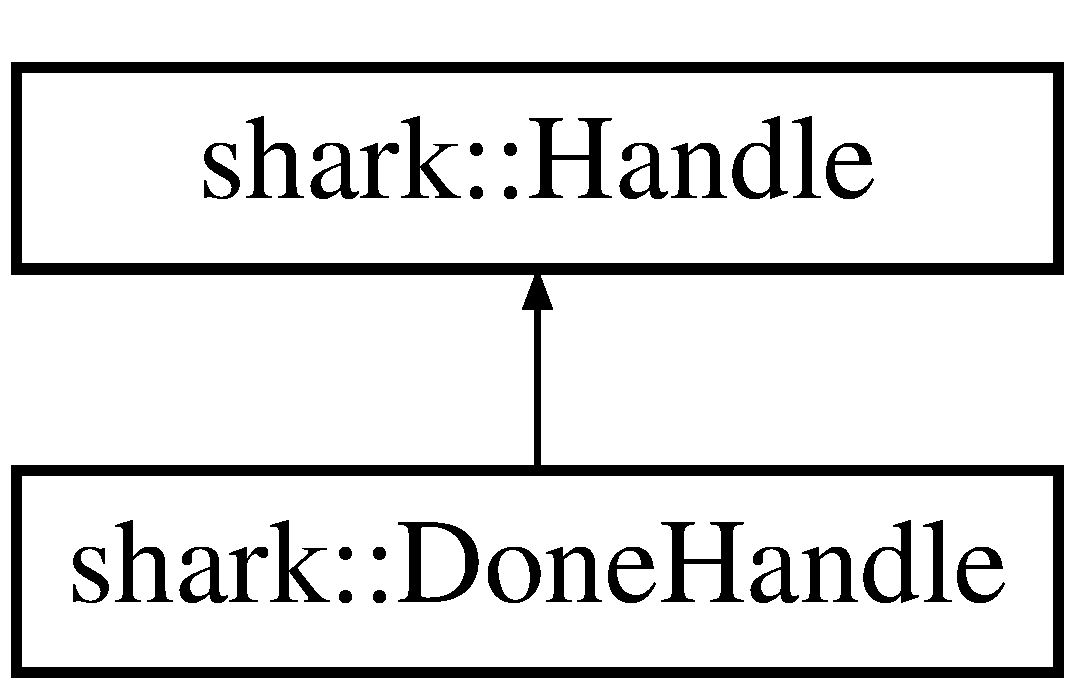
\includegraphics[height=2.000000cm]{classshark_1_1_done_handle}
\end{center}
\end{figure}
\subsection*{Public Member Functions}
\begin{DoxyCompactItemize}
\item 
\hyperlink{classshark_1_1_done_handle_ad4007e3e95525b9f6ff20738b1eee4e3}{Done\+Handle} ()
\item 
virtual \hyperlink{classshark_1_1_done_handle_a2b414f29067919ac09cc37fabf22e716}{$\sim$\+Done\+Handle} ()
\item 
virtual bool \hyperlink{classshark_1_1_done_handle_aa2207dc4b61f0bffcbfb56aa9f9b0b46}{test} ()
\item 
virtual void \hyperlink{classshark_1_1_done_handle_a99b4b58b01738073650b9c452e35b7e8}{wait} ()
\end{DoxyCompactItemize}
\subsection*{Additional Inherited Members}


\subsection{Detailed Description}


Definition at line 29 of file future.\+hpp.



\subsection{Constructor \& Destructor Documentation}
\hypertarget{classshark_1_1_done_handle_ad4007e3e95525b9f6ff20738b1eee4e3}{}\label{classshark_1_1_done_handle_ad4007e3e95525b9f6ff20738b1eee4e3} 
\index{shark\+::\+Done\+Handle@{shark\+::\+Done\+Handle}!Done\+Handle@{Done\+Handle}}
\index{Done\+Handle@{Done\+Handle}!shark\+::\+Done\+Handle@{shark\+::\+Done\+Handle}}
\subsubsection{\texorpdfstring{Done\+Handle()}{DoneHandle()}}
{\footnotesize\ttfamily Done\+Handle\+::\+Done\+Handle (\begin{DoxyParamCaption}{ }\end{DoxyParamCaption})}



Definition at line 30 of file future.\+cpp.


\begin{DoxyCode}
30                        \{
31 \}
\end{DoxyCode}
\hypertarget{classshark_1_1_done_handle_a2b414f29067919ac09cc37fabf22e716}{}\label{classshark_1_1_done_handle_a2b414f29067919ac09cc37fabf22e716} 
\index{shark\+::\+Done\+Handle@{shark\+::\+Done\+Handle}!````~Done\+Handle@{$\sim$\+Done\+Handle}}
\index{````~Done\+Handle@{$\sim$\+Done\+Handle}!shark\+::\+Done\+Handle@{shark\+::\+Done\+Handle}}
\subsubsection{\texorpdfstring{$\sim$\+Done\+Handle()}{~DoneHandle()}}
{\footnotesize\ttfamily Done\+Handle\+::$\sim$\+Done\+Handle (\begin{DoxyParamCaption}{ }\end{DoxyParamCaption})\hspace{0.3cm}{\ttfamily [virtual]}}



Definition at line 33 of file future.\+cpp.


\begin{DoxyCode}
33                         \{
34 \}
\end{DoxyCode}


\subsection{Member Function Documentation}
\hypertarget{classshark_1_1_done_handle_aa2207dc4b61f0bffcbfb56aa9f9b0b46}{}\label{classshark_1_1_done_handle_aa2207dc4b61f0bffcbfb56aa9f9b0b46} 
\index{shark\+::\+Done\+Handle@{shark\+::\+Done\+Handle}!test@{test}}
\index{test@{test}!shark\+::\+Done\+Handle@{shark\+::\+Done\+Handle}}
\subsubsection{\texorpdfstring{test()}{test()}}
{\footnotesize\ttfamily bool Done\+Handle\+::test (\begin{DoxyParamCaption}{ }\end{DoxyParamCaption})\hspace{0.3cm}{\ttfamily [virtual]}}



Implements \hyperlink{classshark_1_1_handle_a79ac46bc643e22c2a1fb28d45634fa68}{shark\+::\+Handle}.



Definition at line 36 of file future.\+cpp.


\begin{DoxyCode}
36                       \{
37     \textcolor{keywordflow}{return} \textcolor{keyword}{true};
38 \}
\end{DoxyCode}
\hypertarget{classshark_1_1_done_handle_a99b4b58b01738073650b9c452e35b7e8}{}\label{classshark_1_1_done_handle_a99b4b58b01738073650b9c452e35b7e8} 
\index{shark\+::\+Done\+Handle@{shark\+::\+Done\+Handle}!wait@{wait}}
\index{wait@{wait}!shark\+::\+Done\+Handle@{shark\+::\+Done\+Handle}}
\subsubsection{\texorpdfstring{wait()}{wait()}}
{\footnotesize\ttfamily void Done\+Handle\+::wait (\begin{DoxyParamCaption}{ }\end{DoxyParamCaption})\hspace{0.3cm}{\ttfamily [virtual]}}



Implements \hyperlink{classshark_1_1_handle_a36117a898368730a1619a1a771cca424}{shark\+::\+Handle}.



Definition at line 40 of file future.\+cpp.


\begin{DoxyCode}
40                       \{
41 \}
\end{DoxyCode}


The documentation for this class was generated from the following files\+:\begin{DoxyCompactItemize}
\item 
include/shark/\hyperlink{future_8hpp}{future.\+hpp}\item 
src/\hyperlink{future_8cpp}{future.\+cpp}\end{DoxyCompactItemize}

\hypertarget{classshark_1_1ndim_1_1_eq}{}\section{shark\+:\+:ndim\+:\+:Eq$<$ S1, S2 $>$ Class Template Reference}
\label{classshark_1_1ndim_1_1_eq}\index{shark\+::ndim\+::\+Eq$<$ S1, S2 $>$@{shark\+::ndim\+::\+Eq$<$ S1, S2 $>$}}


{\ttfamily \#include $<$expr.\+hpp$>$}

\subsection*{Public Member Functions}
\begin{DoxyCompactItemize}
\item 
auto \hyperlink{classshark_1_1ndim_1_1_eq_a3d6db8cfe90353585a4ebcd720e07abb}{operator()} (const typename S1\+::accessor \&a1, const typename S2\+::accessor \&a2, \hyperlink{structshark_1_1ndim_1_1coords}{coords}$<$ S1\+::number\+\_\+of\+\_\+dimensions $>$ ii) const -\/$>$ decltype(a1(ii)==a2(ii))
\end{DoxyCompactItemize}


\subsection{Detailed Description}
\subsubsection*{template$<$typename S1, typename S2$>$\newline
class shark\+::ndim\+::\+Eq$<$ S1, S2 $>$}

Comparisons 

Definition at line 888 of file expr.\+hpp.



\subsection{Member Function Documentation}
\hypertarget{classshark_1_1ndim_1_1_eq_a3d6db8cfe90353585a4ebcd720e07abb}{}\label{classshark_1_1ndim_1_1_eq_a3d6db8cfe90353585a4ebcd720e07abb} 
\index{shark\+::ndim\+::\+Eq@{shark\+::ndim\+::\+Eq}!operator()@{operator()}}
\index{operator()@{operator()}!shark\+::ndim\+::\+Eq@{shark\+::ndim\+::\+Eq}}
\subsubsection{\texorpdfstring{operator()()}{operator()()}}
{\footnotesize\ttfamily template$<$typename S1 , typename S2 $>$ \\
auto \hyperlink{classshark_1_1ndim_1_1_eq}{shark\+::ndim\+::\+Eq}$<$ S1, S2 $>$\+::operator() (\begin{DoxyParamCaption}\item[{const typename S1\+::accessor \&}]{a1,  }\item[{const typename S2\+::accessor \&}]{a2,  }\item[{\hyperlink{structshark_1_1ndim_1_1coords}{coords}$<$ S1\+::number\+\_\+of\+\_\+dimensions $>$}]{ii }\end{DoxyParamCaption}) const -\/$>$ decltype(a1(ii) == a2(ii)) \hspace{0.3cm}{\ttfamily [inline]}}



Definition at line 890 of file expr.\+hpp.


\begin{DoxyCode}
890                                                                                                            
                                                            \{
891                 \textcolor{keywordflow}{return} a1(ii) == a2(ii);
892             \}
\end{DoxyCode}


The documentation for this class was generated from the following file\+:\begin{DoxyCompactItemize}
\item 
include/shark/\hyperlink{expr_8hpp}{expr.\+hpp}\end{DoxyCompactItemize}

\hypertarget{classshark_1_1ndim_1_1_boundary_1_1fixed__type}{}\section{shark\+:\+:ndim\+:\+:Boundary$<$ ndim, T $>$\+:\+:fixed\+\_\+type Class Reference}
\label{classshark_1_1ndim_1_1_boundary_1_1fixed__type}\index{shark\+::ndim\+::\+Boundary$<$ ndim, T $>$\+::fixed\+\_\+type@{shark\+::ndim\+::\+Boundary$<$ ndim, T $>$\+::fixed\+\_\+type}}
Inheritance diagram for shark\+:\+:ndim\+:\+:Boundary$<$ ndim, T $>$\+:\+:fixed\+\_\+type\+:\begin{figure}[H]
\begin{center}
\leavevmode
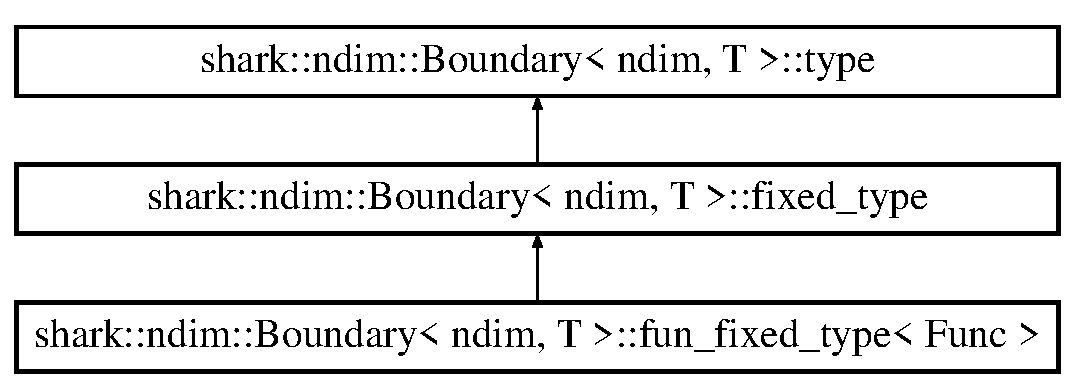
\includegraphics[height=3.000000cm]{classshark_1_1ndim_1_1_boundary_1_1fixed__type}
\end{center}
\end{figure}
\subsection*{Public Member Functions}
\begin{DoxyCompactItemize}
\item 
virtual void \hyperlink{classshark_1_1ndim_1_1_boundary_1_1fixed__type_ad94ec2994049c5107d0ea5d24bf8cff3}{set} (\hyperlink{classshark_1_1ndim_1_1_access}{Access}$<$ ndim, T $>$ \&a, \hyperlink{structshark_1_1ndim_1_1coords__range}{coords\+\_\+range}$<$ ndim $>$ r) const =0
\end{DoxyCompactItemize}


\subsection{Detailed Description}
\subsubsection*{template$<$int ndim, typename T$>$\newline
class shark\+::ndim\+::\+Boundary$<$ ndim, T $>$\+::fixed\+\_\+type}



Definition at line 42 of file boundary.\+hpp.



\subsection{Member Function Documentation}
\hypertarget{classshark_1_1ndim_1_1_boundary_1_1fixed__type_ad94ec2994049c5107d0ea5d24bf8cff3}{}\label{classshark_1_1ndim_1_1_boundary_1_1fixed__type_ad94ec2994049c5107d0ea5d24bf8cff3} 
\index{shark\+::ndim\+::\+Boundary\+::fixed\+\_\+type@{shark\+::ndim\+::\+Boundary\+::fixed\+\_\+type}!set@{set}}
\index{set@{set}!shark\+::ndim\+::\+Boundary\+::fixed\+\_\+type@{shark\+::ndim\+::\+Boundary\+::fixed\+\_\+type}}
\subsubsection{\texorpdfstring{set()}{set()}}
{\footnotesize\ttfamily template$<$int ndim, typename T$>$ \\
virtual void \hyperlink{classshark_1_1ndim_1_1_boundary}{shark\+::ndim\+::\+Boundary}$<$ ndim, T $>$\+::fixed\+\_\+type\+::set (\begin{DoxyParamCaption}\item[{\hyperlink{classshark_1_1ndim_1_1_access}{Access}$<$ ndim, T $>$ \&}]{a,  }\item[{\hyperlink{structshark_1_1ndim_1_1coords__range}{coords\+\_\+range}$<$ ndim $>$}]{r }\end{DoxyParamCaption}) const\hspace{0.3cm}{\ttfamily [pure virtual]}}



Implemented in \hyperlink{classshark_1_1ndim_1_1_boundary_1_1fun__fixed__type_adc9d38ff40b75decf5790ad6f701f3ad}{shark\+::ndim\+::\+Boundary$<$ ndim, T $>$\+::fun\+\_\+fixed\+\_\+type$<$ Func $>$}.



The documentation for this class was generated from the following file\+:\begin{DoxyCompactItemize}
\item 
include/shark/\hyperlink{boundary_8hpp}{boundary.\+hpp}\end{DoxyCompactItemize}

\hypertarget{classshark_1_1ndim_1_1_boundary_1_1fun__fixed__type}{}\section{shark\+:\+:ndim\+:\+:Boundary$<$ ndim, T $>$\+:\+:fun\+\_\+fixed\+\_\+type$<$ Func $>$ Class Template Reference}
\label{classshark_1_1ndim_1_1_boundary_1_1fun__fixed__type}\index{shark\+::ndim\+::\+Boundary$<$ ndim, T $>$\+::fun\+\_\+fixed\+\_\+type$<$ Func $>$@{shark\+::ndim\+::\+Boundary$<$ ndim, T $>$\+::fun\+\_\+fixed\+\_\+type$<$ Func $>$}}
Inheritance diagram for shark\+:\+:ndim\+:\+:Boundary$<$ ndim, T $>$\+:\+:fun\+\_\+fixed\+\_\+type$<$ Func $>$\+:\begin{figure}[H]
\begin{center}
\leavevmode
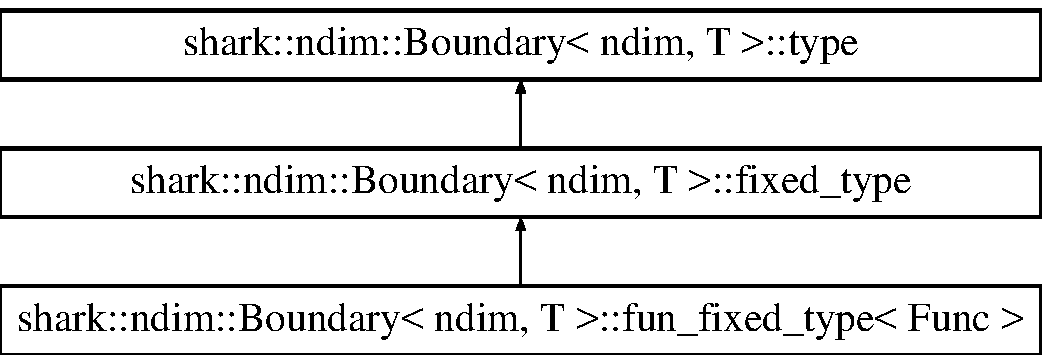
\includegraphics[height=3.000000cm]{classshark_1_1ndim_1_1_boundary_1_1fun__fixed__type}
\end{center}
\end{figure}
\subsection*{Public Member Functions}
\begin{DoxyCompactItemize}
\item 
\hyperlink{classshark_1_1ndim_1_1_boundary_1_1fun__fixed__type_a90a285a78f698d32d080910c0748ecc0}{fun\+\_\+fixed\+\_\+type} (const Func \&\hyperlink{classshark_1_1ndim_1_1_boundary_1_1fun__fixed__type_a968985106f368116b458500c16c4476f}{f})
\item 
virtual \hyperlink{classshark_1_1ndim_1_1_boundary_1_1fun__fixed__type_ae72b49516804b9d47bdc29917d7249bf}{$\sim$fun\+\_\+fixed\+\_\+type} ()
\item 
virtual \hyperlink{classshark_1_1ndim_1_1_boundary_1_1fun__fixed__type}{fun\+\_\+fixed\+\_\+type}$<$ Func $>$ $\ast$ \hyperlink{classshark_1_1ndim_1_1_boundary_1_1fun__fixed__type_a54ad8e702f2f3ff9403d43bfb7b38411}{clone} () const
\item 
virtual void \hyperlink{classshark_1_1ndim_1_1_boundary_1_1fun__fixed__type_adc9d38ff40b75decf5790ad6f701f3ad}{set} (\hyperlink{classshark_1_1ndim_1_1_access}{Access}$<$ ndim, T $>$ \&a, \hyperlink{structshark_1_1ndim_1_1coords__range}{coords\+\_\+range}$<$ ndim $>$ r) const
\end{DoxyCompactItemize}
\subsection*{Private Attributes}
\begin{DoxyCompactItemize}
\item 
Func \hyperlink{classshark_1_1ndim_1_1_boundary_1_1fun__fixed__type_a968985106f368116b458500c16c4476f}{f}
\end{DoxyCompactItemize}


\subsection{Detailed Description}
\subsubsection*{template$<$int ndim, typename T$>$\newline
template$<$typename Func$>$\newline
class shark\+::ndim\+::\+Boundary$<$ ndim, T $>$\+::fun\+\_\+fixed\+\_\+type$<$ Func $>$}



Definition at line 53 of file boundary.\+hpp.



\subsection{Constructor \& Destructor Documentation}
\hypertarget{classshark_1_1ndim_1_1_boundary_1_1fun__fixed__type_a90a285a78f698d32d080910c0748ecc0}{}\label{classshark_1_1ndim_1_1_boundary_1_1fun__fixed__type_a90a285a78f698d32d080910c0748ecc0} 
\index{shark\+::ndim\+::\+Boundary\+::fun\+\_\+fixed\+\_\+type@{shark\+::ndim\+::\+Boundary\+::fun\+\_\+fixed\+\_\+type}!fun\+\_\+fixed\+\_\+type@{fun\+\_\+fixed\+\_\+type}}
\index{fun\+\_\+fixed\+\_\+type@{fun\+\_\+fixed\+\_\+type}!shark\+::ndim\+::\+Boundary\+::fun\+\_\+fixed\+\_\+type@{shark\+::ndim\+::\+Boundary\+::fun\+\_\+fixed\+\_\+type}}
\subsubsection{\texorpdfstring{fun\+\_\+fixed\+\_\+type()}{fun\_fixed\_type()}}
{\footnotesize\ttfamily template$<$int ndim, typename T $>$ \\
template$<$typename Func $>$ \\
\hyperlink{classshark_1_1ndim_1_1_boundary}{shark\+::ndim\+::\+Boundary}$<$ ndim, T $>$\+::\hyperlink{classshark_1_1ndim_1_1_boundary_1_1fun__fixed__type}{fun\+\_\+fixed\+\_\+type}$<$ Func $>$\+::\hyperlink{classshark_1_1ndim_1_1_boundary_1_1fun__fixed__type}{fun\+\_\+fixed\+\_\+type} (\begin{DoxyParamCaption}\item[{const Func \&}]{f }\end{DoxyParamCaption})}



Definition at line 123 of file boundary.\+hpp.


\begin{DoxyCode}
123 : \hyperlink{classshark_1_1ndim_1_1_boundary_1_1fun__fixed__type_a968985106f368116b458500c16c4476f}{f}(\hyperlink{classshark_1_1ndim_1_1_boundary_1_1fun__fixed__type_a968985106f368116b458500c16c4476f}{f}) \{ \}
\end{DoxyCode}
\hypertarget{classshark_1_1ndim_1_1_boundary_1_1fun__fixed__type_ae72b49516804b9d47bdc29917d7249bf}{}\label{classshark_1_1ndim_1_1_boundary_1_1fun__fixed__type_ae72b49516804b9d47bdc29917d7249bf} 
\index{shark\+::ndim\+::\+Boundary\+::fun\+\_\+fixed\+\_\+type@{shark\+::ndim\+::\+Boundary\+::fun\+\_\+fixed\+\_\+type}!````~fun\+\_\+fixed\+\_\+type@{$\sim$fun\+\_\+fixed\+\_\+type}}
\index{````~fun\+\_\+fixed\+\_\+type@{$\sim$fun\+\_\+fixed\+\_\+type}!shark\+::ndim\+::\+Boundary\+::fun\+\_\+fixed\+\_\+type@{shark\+::ndim\+::\+Boundary\+::fun\+\_\+fixed\+\_\+type}}
\subsubsection{\texorpdfstring{$\sim$fun\+\_\+fixed\+\_\+type()}{~fun\_fixed\_type()}}
{\footnotesize\ttfamily template$<$int ndim, typename T $>$ \\
template$<$typename Func $>$ \\
\hyperlink{classshark_1_1ndim_1_1_boundary}{shark\+::ndim\+::\+Boundary}$<$ ndim, T $>$\+::\hyperlink{classshark_1_1ndim_1_1_boundary_1_1fun__fixed__type}{fun\+\_\+fixed\+\_\+type}$<$ Func $>$\+::$\sim$\hyperlink{classshark_1_1ndim_1_1_boundary_1_1fun__fixed__type}{fun\+\_\+fixed\+\_\+type} (\begin{DoxyParamCaption}{ }\end{DoxyParamCaption})\hspace{0.3cm}{\ttfamily [virtual]}}



Definition at line 126 of file boundary.\+hpp.


\begin{DoxyCode}
126 \{ \}
\end{DoxyCode}


\subsection{Member Function Documentation}
\hypertarget{classshark_1_1ndim_1_1_boundary_1_1fun__fixed__type_a54ad8e702f2f3ff9403d43bfb7b38411}{}\label{classshark_1_1ndim_1_1_boundary_1_1fun__fixed__type_a54ad8e702f2f3ff9403d43bfb7b38411} 
\index{shark\+::ndim\+::\+Boundary\+::fun\+\_\+fixed\+\_\+type@{shark\+::ndim\+::\+Boundary\+::fun\+\_\+fixed\+\_\+type}!clone@{clone}}
\index{clone@{clone}!shark\+::ndim\+::\+Boundary\+::fun\+\_\+fixed\+\_\+type@{shark\+::ndim\+::\+Boundary\+::fun\+\_\+fixed\+\_\+type}}
\subsubsection{\texorpdfstring{clone()}{clone()}}
{\footnotesize\ttfamily template$<$int ndim, typename T $>$ \\
template$<$typename Func $>$ \\
\hyperlink{classshark_1_1ndim_1_1_boundary}{Boundary}$<$ ndim, T $>$\+::\hyperlink{classshark_1_1ndim_1_1_boundary_1_1fun__fixed__type}{fun\+\_\+fixed\+\_\+type}$<$ Func $>$ $\ast$ \hyperlink{classshark_1_1ndim_1_1_boundary}{shark\+::ndim\+::\+Boundary}$<$ ndim, T $>$\+::\hyperlink{classshark_1_1ndim_1_1_boundary_1_1fun__fixed__type}{fun\+\_\+fixed\+\_\+type}$<$ Func $>$\+::clone (\begin{DoxyParamCaption}{ }\end{DoxyParamCaption}) const\hspace{0.3cm}{\ttfamily [virtual]}}



Reimplemented from \hyperlink{classshark_1_1ndim_1_1_boundary_1_1type_a5651988ce3a6c229009d3fa849e820dc}{shark\+::ndim\+::\+Boundary$<$ ndim, T $>$\+::type}.



Definition at line 129 of file boundary.\+hpp.


\begin{DoxyCode}
129                                                                                                 \{
130             \textcolor{keywordflow}{return} \textcolor{keyword}{new} fun\_fixed\_type<Func>(\hyperlink{classshark_1_1ndim_1_1_boundary_1_1fun__fixed__type_a968985106f368116b458500c16c4476f}{f});
131         \}
\end{DoxyCode}
\hypertarget{classshark_1_1ndim_1_1_boundary_1_1fun__fixed__type_adc9d38ff40b75decf5790ad6f701f3ad}{}\label{classshark_1_1ndim_1_1_boundary_1_1fun__fixed__type_adc9d38ff40b75decf5790ad6f701f3ad} 
\index{shark\+::ndim\+::\+Boundary\+::fun\+\_\+fixed\+\_\+type@{shark\+::ndim\+::\+Boundary\+::fun\+\_\+fixed\+\_\+type}!set@{set}}
\index{set@{set}!shark\+::ndim\+::\+Boundary\+::fun\+\_\+fixed\+\_\+type@{shark\+::ndim\+::\+Boundary\+::fun\+\_\+fixed\+\_\+type}}
\subsubsection{\texorpdfstring{set()}{set()}}
{\footnotesize\ttfamily template$<$int ndim, typename T $>$ \\
template$<$typename Func $>$ \\
void \hyperlink{classshark_1_1ndim_1_1_boundary}{shark\+::ndim\+::\+Boundary}$<$ ndim, T $>$\+::\hyperlink{classshark_1_1ndim_1_1_boundary_1_1fun__fixed__type}{fun\+\_\+fixed\+\_\+type}$<$ Func $>$\+::set (\begin{DoxyParamCaption}\item[{\hyperlink{classshark_1_1ndim_1_1_access}{Access}$<$ ndim, T $>$ \&}]{a,  }\item[{\hyperlink{structshark_1_1ndim_1_1coords__range}{coords\+\_\+range}$<$ ndim $>$}]{r }\end{DoxyParamCaption}) const\hspace{0.3cm}{\ttfamily [virtual]}}



Implements \hyperlink{classshark_1_1ndim_1_1_boundary_1_1fixed__type_ad94ec2994049c5107d0ea5d24bf8cff3}{shark\+::ndim\+::\+Boundary$<$ ndim, T $>$\+::fixed\+\_\+type}.



Definition at line 134 of file boundary.\+hpp.


\begin{DoxyCode}
134                                                                                                     \{
135             r.for\_each([\textcolor{keyword}{this},&a](coords<ndim> ii) \{
136                 a(ii) = \hyperlink{classshark_1_1ndim_1_1_boundary_1_1fun__fixed__type_a968985106f368116b458500c16c4476f}{f}(ii);
137             \});
138         \}
\end{DoxyCode}


\subsection{Member Data Documentation}
\hypertarget{classshark_1_1ndim_1_1_boundary_1_1fun__fixed__type_a968985106f368116b458500c16c4476f}{}\label{classshark_1_1ndim_1_1_boundary_1_1fun__fixed__type_a968985106f368116b458500c16c4476f} 
\index{shark\+::ndim\+::\+Boundary\+::fun\+\_\+fixed\+\_\+type@{shark\+::ndim\+::\+Boundary\+::fun\+\_\+fixed\+\_\+type}!f@{f}}
\index{f@{f}!shark\+::ndim\+::\+Boundary\+::fun\+\_\+fixed\+\_\+type@{shark\+::ndim\+::\+Boundary\+::fun\+\_\+fixed\+\_\+type}}
\subsubsection{\texorpdfstring{f}{f}}
{\footnotesize\ttfamily template$<$int ndim, typename T$>$ \\
template$<$typename Func$>$ \\
Func \hyperlink{classshark_1_1ndim_1_1_boundary}{shark\+::ndim\+::\+Boundary}$<$ ndim, T $>$\+::\hyperlink{classshark_1_1ndim_1_1_boundary_1_1fun__fixed__type}{fun\+\_\+fixed\+\_\+type}$<$ Func $>$\+::f\hspace{0.3cm}{\ttfamily [private]}}



Definition at line 54 of file boundary.\+hpp.



The documentation for this class was generated from the following file\+:\begin{DoxyCompactItemize}
\item 
include/shark/\hyperlink{boundary_8hpp}{boundary.\+hpp}\end{DoxyCompactItemize}

\hypertarget{classshark_1_1ndim_1_1_boundary_1_1fun__general__type}{}\section{shark\+:\+:ndim\+:\+:Boundary$<$ ndim, T $>$\+:\+:fun\+\_\+general\+\_\+type$<$ Func $>$ Class Template Reference}
\label{classshark_1_1ndim_1_1_boundary_1_1fun__general__type}\index{shark\+::ndim\+::\+Boundary$<$ ndim, T $>$\+::fun\+\_\+general\+\_\+type$<$ Func $>$@{shark\+::ndim\+::\+Boundary$<$ ndim, T $>$\+::fun\+\_\+general\+\_\+type$<$ Func $>$}}
Inheritance diagram for shark\+:\+:ndim\+:\+:Boundary$<$ ndim, T $>$\+:\+:fun\+\_\+general\+\_\+type$<$ Func $>$\+:\begin{figure}[H]
\begin{center}
\leavevmode
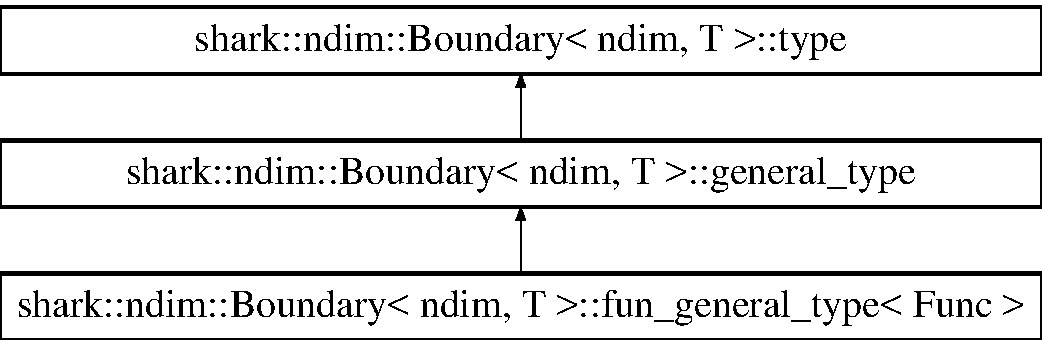
\includegraphics[height=3.000000cm]{classshark_1_1ndim_1_1_boundary_1_1fun__general__type}
\end{center}
\end{figure}
\subsection*{Public Member Functions}
\begin{DoxyCompactItemize}
\item 
\hyperlink{classshark_1_1ndim_1_1_boundary_1_1fun__general__type_af5d09f114b529e82be303a9b9896a84b}{fun\+\_\+general\+\_\+type} (const Func \&\hyperlink{classshark_1_1ndim_1_1_boundary_1_1fun__general__type_a7a2449e92b694dd4d966e17c4d999a91}{f})
\item 
virtual \hyperlink{classshark_1_1ndim_1_1_boundary_1_1fun__general__type_a05fd22999b9a79dbfecca14e1014d654}{$\sim$fun\+\_\+general\+\_\+type} ()
\item 
virtual \hyperlink{classshark_1_1ndim_1_1_boundary_1_1fun__general__type}{fun\+\_\+general\+\_\+type}$<$ Func $>$ $\ast$ \hyperlink{classshark_1_1ndim_1_1_boundary_1_1fun__general__type_a2a2ebd25aa8dcb4960c28db87680e7c6}{clone} () const
\item 
virtual void \hyperlink{classshark_1_1ndim_1_1_boundary_1_1fun__general__type_a7f5d89a026065de5a42b757ce507a70f}{set} (\hyperlink{classshark_1_1ndim_1_1_access}{Access}$<$ ndim, T $>$ \&a, \hyperlink{structshark_1_1ndim_1_1coords__range}{coords\+\_\+range}$<$ ndim $>$ r, long k) const
\end{DoxyCompactItemize}
\subsection*{Private Attributes}
\begin{DoxyCompactItemize}
\item 
Func \hyperlink{classshark_1_1ndim_1_1_boundary_1_1fun__general__type_a7a2449e92b694dd4d966e17c4d999a91}{f}
\end{DoxyCompactItemize}


\subsection{Detailed Description}
\subsubsection*{template$<$int ndim, typename T$>$\newline
template$<$typename Func$>$\newline
class shark\+::ndim\+::\+Boundary$<$ ndim, T $>$\+::fun\+\_\+general\+\_\+type$<$ Func $>$}



Definition at line 63 of file boundary.\+hpp.



\subsection{Constructor \& Destructor Documentation}
\hypertarget{classshark_1_1ndim_1_1_boundary_1_1fun__general__type_af5d09f114b529e82be303a9b9896a84b}{}\label{classshark_1_1ndim_1_1_boundary_1_1fun__general__type_af5d09f114b529e82be303a9b9896a84b} 
\index{shark\+::ndim\+::\+Boundary\+::fun\+\_\+general\+\_\+type@{shark\+::ndim\+::\+Boundary\+::fun\+\_\+general\+\_\+type}!fun\+\_\+general\+\_\+type@{fun\+\_\+general\+\_\+type}}
\index{fun\+\_\+general\+\_\+type@{fun\+\_\+general\+\_\+type}!shark\+::ndim\+::\+Boundary\+::fun\+\_\+general\+\_\+type@{shark\+::ndim\+::\+Boundary\+::fun\+\_\+general\+\_\+type}}
\subsubsection{\texorpdfstring{fun\+\_\+general\+\_\+type()}{fun\_general\_type()}}
{\footnotesize\ttfamily template$<$int ndim, typename T $>$ \\
template$<$typename Func $>$ \\
\hyperlink{classshark_1_1ndim_1_1_boundary}{shark\+::ndim\+::\+Boundary}$<$ ndim, T $>$\+::\hyperlink{classshark_1_1ndim_1_1_boundary_1_1fun__general__type}{fun\+\_\+general\+\_\+type}$<$ Func $>$\+::\hyperlink{classshark_1_1ndim_1_1_boundary_1_1fun__general__type}{fun\+\_\+general\+\_\+type} (\begin{DoxyParamCaption}\item[{const Func \&}]{f }\end{DoxyParamCaption})}



Definition at line 141 of file boundary.\+hpp.


\begin{DoxyCode}
141 : \hyperlink{classshark_1_1ndim_1_1_boundary_1_1fun__general__type_a7a2449e92b694dd4d966e17c4d999a91}{f}(\hyperlink{classshark_1_1ndim_1_1_boundary_1_1fun__general__type_a7a2449e92b694dd4d966e17c4d999a91}{f}) \{ \}
\end{DoxyCode}
\hypertarget{classshark_1_1ndim_1_1_boundary_1_1fun__general__type_a05fd22999b9a79dbfecca14e1014d654}{}\label{classshark_1_1ndim_1_1_boundary_1_1fun__general__type_a05fd22999b9a79dbfecca14e1014d654} 
\index{shark\+::ndim\+::\+Boundary\+::fun\+\_\+general\+\_\+type@{shark\+::ndim\+::\+Boundary\+::fun\+\_\+general\+\_\+type}!````~fun\+\_\+general\+\_\+type@{$\sim$fun\+\_\+general\+\_\+type}}
\index{````~fun\+\_\+general\+\_\+type@{$\sim$fun\+\_\+general\+\_\+type}!shark\+::ndim\+::\+Boundary\+::fun\+\_\+general\+\_\+type@{shark\+::ndim\+::\+Boundary\+::fun\+\_\+general\+\_\+type}}
\subsubsection{\texorpdfstring{$\sim$fun\+\_\+general\+\_\+type()}{~fun\_general\_type()}}
{\footnotesize\ttfamily template$<$int ndim, typename T $>$ \\
template$<$typename Func $>$ \\
\hyperlink{classshark_1_1ndim_1_1_boundary}{shark\+::ndim\+::\+Boundary}$<$ ndim, T $>$\+::\hyperlink{classshark_1_1ndim_1_1_boundary_1_1fun__general__type}{fun\+\_\+general\+\_\+type}$<$ Func $>$\+::$\sim$\hyperlink{classshark_1_1ndim_1_1_boundary_1_1fun__general__type}{fun\+\_\+general\+\_\+type} (\begin{DoxyParamCaption}{ }\end{DoxyParamCaption})\hspace{0.3cm}{\ttfamily [virtual]}}



Definition at line 144 of file boundary.\+hpp.


\begin{DoxyCode}
144 \{ \}
\end{DoxyCode}


\subsection{Member Function Documentation}
\hypertarget{classshark_1_1ndim_1_1_boundary_1_1fun__general__type_a2a2ebd25aa8dcb4960c28db87680e7c6}{}\label{classshark_1_1ndim_1_1_boundary_1_1fun__general__type_a2a2ebd25aa8dcb4960c28db87680e7c6} 
\index{shark\+::ndim\+::\+Boundary\+::fun\+\_\+general\+\_\+type@{shark\+::ndim\+::\+Boundary\+::fun\+\_\+general\+\_\+type}!clone@{clone}}
\index{clone@{clone}!shark\+::ndim\+::\+Boundary\+::fun\+\_\+general\+\_\+type@{shark\+::ndim\+::\+Boundary\+::fun\+\_\+general\+\_\+type}}
\subsubsection{\texorpdfstring{clone()}{clone()}}
{\footnotesize\ttfamily template$<$int ndim, typename T $>$ \\
template$<$typename Func $>$ \\
\hyperlink{classshark_1_1ndim_1_1_boundary}{Boundary}$<$ ndim, T $>$\+::\hyperlink{classshark_1_1ndim_1_1_boundary_1_1fun__general__type}{fun\+\_\+general\+\_\+type}$<$ Func $>$ $\ast$ \hyperlink{classshark_1_1ndim_1_1_boundary}{shark\+::ndim\+::\+Boundary}$<$ ndim, T $>$\+::\hyperlink{classshark_1_1ndim_1_1_boundary_1_1fun__general__type}{fun\+\_\+general\+\_\+type}$<$ Func $>$\+::clone (\begin{DoxyParamCaption}{ }\end{DoxyParamCaption}) const\hspace{0.3cm}{\ttfamily [virtual]}}



Reimplemented from \hyperlink{classshark_1_1ndim_1_1_boundary_1_1type_a5651988ce3a6c229009d3fa849e820dc}{shark\+::ndim\+::\+Boundary$<$ ndim, T $>$\+::type}.



Definition at line 147 of file boundary.\+hpp.


\begin{DoxyCode}
147                                                                                                     \{
148             \textcolor{keywordflow}{return} \textcolor{keyword}{new} fun\_general\_type<Func>(\hyperlink{classshark_1_1ndim_1_1_boundary_1_1fun__general__type_a7a2449e92b694dd4d966e17c4d999a91}{f});
149         \}
\end{DoxyCode}
\hypertarget{classshark_1_1ndim_1_1_boundary_1_1fun__general__type_a7f5d89a026065de5a42b757ce507a70f}{}\label{classshark_1_1ndim_1_1_boundary_1_1fun__general__type_a7f5d89a026065de5a42b757ce507a70f} 
\index{shark\+::ndim\+::\+Boundary\+::fun\+\_\+general\+\_\+type@{shark\+::ndim\+::\+Boundary\+::fun\+\_\+general\+\_\+type}!set@{set}}
\index{set@{set}!shark\+::ndim\+::\+Boundary\+::fun\+\_\+general\+\_\+type@{shark\+::ndim\+::\+Boundary\+::fun\+\_\+general\+\_\+type}}
\subsubsection{\texorpdfstring{set()}{set()}}
{\footnotesize\ttfamily template$<$int ndim, typename T $>$ \\
template$<$typename Func $>$ \\
void \hyperlink{classshark_1_1ndim_1_1_boundary}{shark\+::ndim\+::\+Boundary}$<$ ndim, T $>$\+::\hyperlink{classshark_1_1ndim_1_1_boundary_1_1fun__general__type}{fun\+\_\+general\+\_\+type}$<$ Func $>$\+::set (\begin{DoxyParamCaption}\item[{\hyperlink{classshark_1_1ndim_1_1_access}{Access}$<$ ndim, T $>$ \&}]{a,  }\item[{\hyperlink{structshark_1_1ndim_1_1coords__range}{coords\+\_\+range}$<$ ndim $>$}]{r,  }\item[{long}]{k }\end{DoxyParamCaption}) const\hspace{0.3cm}{\ttfamily [virtual]}}



Implements \hyperlink{classshark_1_1ndim_1_1_boundary_1_1general__type_ac73340187c707591d7fc1ccbe85c1b19}{shark\+::ndim\+::\+Boundary$<$ ndim, T $>$\+::general\+\_\+type}.



Definition at line 152 of file boundary.\+hpp.


\begin{DoxyCode}
152                                                                                                            
         \{
153             r.for\_each([\textcolor{keyword}{this},&a,k](coords<ndim> ii) \{
154                 a(ii) = \hyperlink{classshark_1_1ndim_1_1_boundary_1_1fun__general__type_a7a2449e92b694dd4d966e17c4d999a91}{f}(k, ii);
155             \});
156         \}
\end{DoxyCode}


\subsection{Member Data Documentation}
\hypertarget{classshark_1_1ndim_1_1_boundary_1_1fun__general__type_a7a2449e92b694dd4d966e17c4d999a91}{}\label{classshark_1_1ndim_1_1_boundary_1_1fun__general__type_a7a2449e92b694dd4d966e17c4d999a91} 
\index{shark\+::ndim\+::\+Boundary\+::fun\+\_\+general\+\_\+type@{shark\+::ndim\+::\+Boundary\+::fun\+\_\+general\+\_\+type}!f@{f}}
\index{f@{f}!shark\+::ndim\+::\+Boundary\+::fun\+\_\+general\+\_\+type@{shark\+::ndim\+::\+Boundary\+::fun\+\_\+general\+\_\+type}}
\subsubsection{\texorpdfstring{f}{f}}
{\footnotesize\ttfamily template$<$int ndim, typename T$>$ \\
template$<$typename Func$>$ \\
Func \hyperlink{classshark_1_1ndim_1_1_boundary}{shark\+::ndim\+::\+Boundary}$<$ ndim, T $>$\+::\hyperlink{classshark_1_1ndim_1_1_boundary_1_1fun__general__type}{fun\+\_\+general\+\_\+type}$<$ Func $>$\+::f\hspace{0.3cm}{\ttfamily [private]}}



Definition at line 64 of file boundary.\+hpp.



The documentation for this class was generated from the following file\+:\begin{DoxyCompactItemize}
\item 
include/shark/\hyperlink{boundary_8hpp}{boundary.\+hpp}\end{DoxyCompactItemize}

\hypertarget{structshark_1_1_future}{}\section{shark\+:\+:Future$<$ T $>$ Struct Template Reference}
\label{structshark_1_1_future}\index{shark\+::\+Future$<$ T $>$@{shark\+::\+Future$<$ T $>$}}


{\ttfamily \#include $<$common.\+hpp$>$}

\subsection*{Public Member Functions}
\begin{DoxyCompactItemize}
\item 
\hyperlink{structshark_1_1_future_a92d1efe967edc2466b85ac14062cde61}{Future} (std\+::shared\+\_\+ptr$<$ \hyperlink{classshark_1_1_handle}{Handle} $>$ \hyperlink{structshark_1_1_future_a54f00db085adbffb18b2e2ab9e3d4b32}{h})
\item 
\hyperlink{structshark_1_1_future_a2c240241a370e1775353f3c4f0f1b3bb}{Future} (std\+::shared\+\_\+ptr$<$ \hyperlink{classshark_1_1_handle}{Handle} $>$ \hyperlink{structshark_1_1_future_a54f00db085adbffb18b2e2ab9e3d4b32}{h}, std\+::unique\+\_\+ptr$<$ T $>$ \&\&\hyperlink{structshark_1_1_future_ad47e70b84ce6303568af0bd6aca991da}{val})
\item 
\hyperlink{structshark_1_1_future_adbc00059974d00508636b062c2062b9b}{Future} ()
\item 
\hyperlink{structshark_1_1_future_aa17ac6c907e9768b69c143d0b4046551}{$\sim$\+Future} ()
\item 
\hyperlink{structshark_1_1_future_a3c76fd022444f58fcc06ee248d81f72b}{Future} (const \hyperlink{structshark_1_1_future}{Future}$<$ T $>$ \&)=delete
\item 
\hyperlink{structshark_1_1_future}{Future}$<$ T $>$ \& \hyperlink{structshark_1_1_future_a45d4c1fdd9602d41f7e07f49b31e5943}{operator=} (const \hyperlink{structshark_1_1_future}{Future}$<$ T $>$ \&)=delete
\item 
\hyperlink{structshark_1_1_future_a6eff07d7db700729f333f86712dd5f07}{Future} (\hyperlink{structshark_1_1_future}{Future}$<$ T $>$ \&\&f)
\item 
\hyperlink{structshark_1_1_future}{Future} \& \hyperlink{structshark_1_1_future_a660602bfa8a6096020931f35f8d7a7a1}{operator=} (\hyperlink{structshark_1_1_future}{Future}$<$ T $>$ \&\&f)
\item 
bool \hyperlink{structshark_1_1_future_abbc3d1456a7c62296de4ec4603efac2a}{test} ()
\item 
const T \& \hyperlink{structshark_1_1_future_a88a411b5cedec34af07b054d15deedc2}{wait} ()
\item 
\hyperlink{common_8hpp_a2eb6f9e0395b47b8d5e3eeae4fe0c116}{I\+N\+L\+I\+NE} \hyperlink{structshark_1_1_future_a2ad40708ac7a1df9e288af5739d513f1}{operator const T \&} ()
\end{DoxyCompactItemize}
\subsection*{Public Attributes}
\begin{DoxyCompactItemize}
\item 
bool \hyperlink{structshark_1_1_future_ae873cf93e919c066f04ff337ce3a21e1}{done}
\item 
std\+::shared\+\_\+ptr$<$ \hyperlink{classshark_1_1_handle}{Handle} $>$ \hyperlink{structshark_1_1_future_a54f00db085adbffb18b2e2ab9e3d4b32}{h}
\item 
std\+::unique\+\_\+ptr$<$ T $>$ \hyperlink{structshark_1_1_future_ad47e70b84ce6303568af0bd6aca991da}{val}
\end{DoxyCompactItemize}
\subsection*{Friends}
\begin{DoxyCompactItemize}
\item 
class \hyperlink{structshark_1_1_future_a8e678e0244c103cad9467c2b743509bb}{shark\+::\+Group}
\end{DoxyCompactItemize}


\subsection{Detailed Description}
\subsubsection*{template$<$typename T$>$\newline
struct shark\+::\+Future$<$ T $>$}

A future value of type T 

Definition at line 153 of file common.\+hpp.



\subsection{Constructor \& Destructor Documentation}
\hypertarget{structshark_1_1_future_a92d1efe967edc2466b85ac14062cde61}{}\label{structshark_1_1_future_a92d1efe967edc2466b85ac14062cde61} 
\index{shark\+::\+Future@{shark\+::\+Future}!Future@{Future}}
\index{Future@{Future}!shark\+::\+Future@{shark\+::\+Future}}
\subsubsection{\texorpdfstring{Future()}{Future()}\hspace{0.1cm}{\footnotesize\ttfamily [1/5]}}
{\footnotesize\ttfamily template$<$typename T$>$ \\
\hyperlink{structshark_1_1_future}{shark\+::\+Future}$<$ T $>$\+::\hyperlink{structshark_1_1_future}{Future} (\begin{DoxyParamCaption}\item[{std\+::shared\+\_\+ptr$<$ \hyperlink{classshark_1_1_handle}{Handle} $>$}]{h }\end{DoxyParamCaption})}

\hypertarget{structshark_1_1_future_a2c240241a370e1775353f3c4f0f1b3bb}{}\label{structshark_1_1_future_a2c240241a370e1775353f3c4f0f1b3bb} 
\index{shark\+::\+Future@{shark\+::\+Future}!Future@{Future}}
\index{Future@{Future}!shark\+::\+Future@{shark\+::\+Future}}
\subsubsection{\texorpdfstring{Future()}{Future()}\hspace{0.1cm}{\footnotesize\ttfamily [2/5]}}
{\footnotesize\ttfamily template$<$typename T$>$ \\
\hyperlink{structshark_1_1_future}{shark\+::\+Future}$<$ T $>$\+::\hyperlink{structshark_1_1_future}{Future} (\begin{DoxyParamCaption}\item[{std\+::shared\+\_\+ptr$<$ \hyperlink{classshark_1_1_handle}{Handle} $>$}]{h,  }\item[{std\+::unique\+\_\+ptr$<$ T $>$ \&\&}]{val }\end{DoxyParamCaption})}

\hypertarget{structshark_1_1_future_adbc00059974d00508636b062c2062b9b}{}\label{structshark_1_1_future_adbc00059974d00508636b062c2062b9b} 
\index{shark\+::\+Future@{shark\+::\+Future}!Future@{Future}}
\index{Future@{Future}!shark\+::\+Future@{shark\+::\+Future}}
\subsubsection{\texorpdfstring{Future()}{Future()}\hspace{0.1cm}{\footnotesize\ttfamily [3/5]}}
{\footnotesize\ttfamily template$<$typename T $>$ \\
Future\+::\+Future (\begin{DoxyParamCaption}{ }\end{DoxyParamCaption})}

Create an inactive \hyperlink{structshark_1_1_future}{Future} 

Definition at line 44 of file future.\+cpp.


\begin{DoxyCode}
44                  : \hyperlink{structshark_1_1_future_ae873cf93e919c066f04ff337ce3a21e1}{done}(\textcolor{keyword}{false}), \hyperlink{structshark_1_1_future_a54f00db085adbffb18b2e2ab9e3d4b32}{h}(), \hyperlink{structshark_1_1_future_ad47e70b84ce6303568af0bd6aca991da}{val}() \{
45 \}
\end{DoxyCode}
\hypertarget{structshark_1_1_future_aa17ac6c907e9768b69c143d0b4046551}{}\label{structshark_1_1_future_aa17ac6c907e9768b69c143d0b4046551} 
\index{shark\+::\+Future@{shark\+::\+Future}!````~Future@{$\sim$\+Future}}
\index{````~Future@{$\sim$\+Future}!shark\+::\+Future@{shark\+::\+Future}}
\subsubsection{\texorpdfstring{$\sim$\+Future()}{~Future()}}
{\footnotesize\ttfamily template$<$typename T $>$ \\
Future\+::$\sim$\+Future (\begin{DoxyParamCaption}{ }\end{DoxyParamCaption})}



Definition at line 51 of file future.\+cpp.


\begin{DoxyCode}
51                    \{
52     assert(!\hyperlink{structshark_1_1_future_a54f00db085adbffb18b2e2ab9e3d4b32}{h} || \hyperlink{structshark_1_1_future_ae873cf93e919c066f04ff337ce3a21e1}{done});
53 \}
\end{DoxyCode}
\hypertarget{structshark_1_1_future_a3c76fd022444f58fcc06ee248d81f72b}{}\label{structshark_1_1_future_a3c76fd022444f58fcc06ee248d81f72b} 
\index{shark\+::\+Future@{shark\+::\+Future}!Future@{Future}}
\index{Future@{Future}!shark\+::\+Future@{shark\+::\+Future}}
\subsubsection{\texorpdfstring{Future()}{Future()}\hspace{0.1cm}{\footnotesize\ttfamily [4/5]}}
{\footnotesize\ttfamily template$<$typename T$>$ \\
\hyperlink{structshark_1_1_future}{shark\+::\+Future}$<$ T $>$\+::\hyperlink{structshark_1_1_future}{Future} (\begin{DoxyParamCaption}\item[{const \hyperlink{structshark_1_1_future}{Future}$<$ T $>$ \&}]{ }\end{DoxyParamCaption})\hspace{0.3cm}{\ttfamily [delete]}}

No copy semantics \hypertarget{structshark_1_1_future_a6eff07d7db700729f333f86712dd5f07}{}\label{structshark_1_1_future_a6eff07d7db700729f333f86712dd5f07} 
\index{shark\+::\+Future@{shark\+::\+Future}!Future@{Future}}
\index{Future@{Future}!shark\+::\+Future@{shark\+::\+Future}}
\subsubsection{\texorpdfstring{Future()}{Future()}\hspace{0.1cm}{\footnotesize\ttfamily [5/5]}}
{\footnotesize\ttfamily template$<$typename T $>$ \\
Future\+::\+Future (\begin{DoxyParamCaption}\item[{\hyperlink{structshark_1_1_future}{Future}$<$ T $>$ \&\&}]{f }\end{DoxyParamCaption})}

Move semantics 

Definition at line 60 of file future.\+cpp.


\begin{DoxyCode}
60                               : \hyperlink{structshark_1_1_future_ae873cf93e919c066f04ff337ce3a21e1}{done}(f.\hyperlink{structshark_1_1_future_ae873cf93e919c066f04ff337ce3a21e1}{done}), \hyperlink{structshark_1_1_future_a54f00db085adbffb18b2e2ab9e3d4b32}{h}(f.\hyperlink{structshark_1_1_future_a54f00db085adbffb18b2e2ab9e3d4b32}{h}), \hyperlink{structshark_1_1_future_ad47e70b84ce6303568af0bd6aca991da}{val}(std::move(f.
      \hyperlink{structshark_1_1_future_ad47e70b84ce6303568af0bd6aca991da}{val})) \{
61 \}
\end{DoxyCode}


\subsection{Member Function Documentation}
\hypertarget{structshark_1_1_future_a2ad40708ac7a1df9e288af5739d513f1}{}\label{structshark_1_1_future_a2ad40708ac7a1df9e288af5739d513f1} 
\index{shark\+::\+Future@{shark\+::\+Future}!operator const T \&@{operator const T \&}}
\index{operator const T \&@{operator const T \&}!shark\+::\+Future@{shark\+::\+Future}}
\subsubsection{\texorpdfstring{operator const T \&()}{operator const T \&()}}
{\footnotesize\ttfamily template$<$typename T $>$ \\
\hyperlink{structshark_1_1_future}{shark\+::\+Future}$<$ T $>$\+::operator const T \& (\begin{DoxyParamCaption}{ }\end{DoxyParamCaption})\hspace{0.3cm}{\ttfamily [inline]}}



Definition at line 85 of file future.\+hpp.


\begin{DoxyCode}
85                                         \{
86         \textcolor{keywordflow}{return} \hyperlink{structshark_1_1_future_a88a411b5cedec34af07b054d15deedc2}{wait}();
87     \}
\end{DoxyCode}
\hypertarget{structshark_1_1_future_a45d4c1fdd9602d41f7e07f49b31e5943}{}\label{structshark_1_1_future_a45d4c1fdd9602d41f7e07f49b31e5943} 
\index{shark\+::\+Future@{shark\+::\+Future}!operator=@{operator=}}
\index{operator=@{operator=}!shark\+::\+Future@{shark\+::\+Future}}
\subsubsection{\texorpdfstring{operator=()}{operator=()}\hspace{0.1cm}{\footnotesize\ttfamily [1/2]}}
{\footnotesize\ttfamily template$<$typename T$>$ \\
\hyperlink{structshark_1_1_future}{Future}$<$T$>$\& \hyperlink{structshark_1_1_future}{shark\+::\+Future}$<$ T $>$\+::operator= (\begin{DoxyParamCaption}\item[{const \hyperlink{structshark_1_1_future}{Future}$<$ T $>$ \&}]{ }\end{DoxyParamCaption})\hspace{0.3cm}{\ttfamily [delete]}}

\hypertarget{structshark_1_1_future_a660602bfa8a6096020931f35f8d7a7a1}{}\label{structshark_1_1_future_a660602bfa8a6096020931f35f8d7a7a1} 
\index{shark\+::\+Future@{shark\+::\+Future}!operator=@{operator=}}
\index{operator=@{operator=}!shark\+::\+Future@{shark\+::\+Future}}
\subsubsection{\texorpdfstring{operator=()}{operator=()}\hspace{0.1cm}{\footnotesize\ttfamily [2/2]}}
{\footnotesize\ttfamily template$<$typename T $>$ \\
\hyperlink{structshark_1_1_future}{Future}$<$ T $>$ \& Future\+::operator= (\begin{DoxyParamCaption}\item[{\hyperlink{structshark_1_1_future}{Future}$<$ T $>$ \&\&}]{f }\end{DoxyParamCaption})}



Definition at line 67 of file future.\+cpp.


\begin{DoxyCode}
67                                              \{
68     \hyperlink{structshark_1_1_future_ae873cf93e919c066f04ff337ce3a21e1}{done} = f.\hyperlink{structshark_1_1_future_ae873cf93e919c066f04ff337ce3a21e1}{done};
69         f.\hyperlink{structshark_1_1_future_ae873cf93e919c066f04ff337ce3a21e1}{done} = \textcolor{keyword}{true};
70     \hyperlink{structshark_1_1_future_a54f00db085adbffb18b2e2ab9e3d4b32}{h} = f.\hyperlink{structshark_1_1_future_a54f00db085adbffb18b2e2ab9e3d4b32}{h};
71     \hyperlink{structshark_1_1_future_ad47e70b84ce6303568af0bd6aca991da}{val} = std::move(f.\hyperlink{structshark_1_1_future_ad47e70b84ce6303568af0bd6aca991da}{val});
72     \textcolor{keywordflow}{return} *\textcolor{keyword}{this};
73 \}
\end{DoxyCode}
\hypertarget{structshark_1_1_future_abbc3d1456a7c62296de4ec4603efac2a}{}\label{structshark_1_1_future_abbc3d1456a7c62296de4ec4603efac2a} 
\index{shark\+::\+Future@{shark\+::\+Future}!test@{test}}
\index{test@{test}!shark\+::\+Future@{shark\+::\+Future}}
\subsubsection{\texorpdfstring{test()}{test()}}
{\footnotesize\ttfamily template$<$typename T $>$ \\
bool Future\+::test (\begin{DoxyParamCaption}{ }\end{DoxyParamCaption})}

Test for completion. Returns immediately. 

Definition at line 97 of file future.\+cpp.


\begin{DoxyCode}
97                      \{
98     \textcolor{keywordflow}{return} \hyperlink{structshark_1_1_future_ae873cf93e919c066f04ff337ce3a21e1}{done} || (\hyperlink{structshark_1_1_future_ae873cf93e919c066f04ff337ce3a21e1}{done} = \hyperlink{structshark_1_1_future_a54f00db085adbffb18b2e2ab9e3d4b32}{h}->test());
99 \}
\end{DoxyCode}
\hypertarget{structshark_1_1_future_a88a411b5cedec34af07b054d15deedc2}{}\label{structshark_1_1_future_a88a411b5cedec34af07b054d15deedc2} 
\index{shark\+::\+Future@{shark\+::\+Future}!wait@{wait}}
\index{wait@{wait}!shark\+::\+Future@{shark\+::\+Future}}
\subsubsection{\texorpdfstring{wait()}{wait()}}
{\footnotesize\ttfamily template$<$typename T $>$ \\
void Future\+::wait (\begin{DoxyParamCaption}{ }\end{DoxyParamCaption})}

Wait for completion and return value. 

Definition at line 106 of file future.\+cpp.


\begin{DoxyCode}
106                          \{
107     \textcolor{keywordflow}{if}(!\hyperlink{structshark_1_1_future_ae873cf93e919c066f04ff337ce3a21e1}{done}) \{
108         \hyperlink{structshark_1_1_future_a54f00db085adbffb18b2e2ab9e3d4b32}{h}->wait();
109         \hyperlink{structshark_1_1_future_ae873cf93e919c066f04ff337ce3a21e1}{done} = \textcolor{keyword}{true};
110     \}
111     \textcolor{keywordflow}{return} *\hyperlink{structshark_1_1_future_ad47e70b84ce6303568af0bd6aca991da}{val};
112 \}
\end{DoxyCode}


\subsection{Friends And Related Function Documentation}
\hypertarget{structshark_1_1_future_a8e678e0244c103cad9467c2b743509bb}{}\label{structshark_1_1_future_a8e678e0244c103cad9467c2b743509bb} 
\index{shark\+::\+Future@{shark\+::\+Future}!shark\+::\+Group@{shark\+::\+Group}}
\index{shark\+::\+Group@{shark\+::\+Group}!shark\+::\+Future@{shark\+::\+Future}}
\subsubsection{\texorpdfstring{shark\+::\+Group}{shark::Group}}
{\footnotesize\ttfamily template$<$typename T$>$ \\
friend class \hyperlink{classshark_1_1_group}{shark\+::\+Group}\hspace{0.3cm}{\ttfamily [friend]}}



Definition at line 42 of file future.\+hpp.



\subsection{Member Data Documentation}
\hypertarget{structshark_1_1_future_ae873cf93e919c066f04ff337ce3a21e1}{}\label{structshark_1_1_future_ae873cf93e919c066f04ff337ce3a21e1} 
\index{shark\+::\+Future@{shark\+::\+Future}!done@{done}}
\index{done@{done}!shark\+::\+Future@{shark\+::\+Future}}
\subsubsection{\texorpdfstring{done}{done}}
{\footnotesize\ttfamily template$<$typename T$>$ \\
bool \hyperlink{structshark_1_1_future}{shark\+::\+Future}$<$ T $>$\+::done}



Definition at line 43 of file future.\+hpp.

\hypertarget{structshark_1_1_future_a54f00db085adbffb18b2e2ab9e3d4b32}{}\label{structshark_1_1_future_a54f00db085adbffb18b2e2ab9e3d4b32} 
\index{shark\+::\+Future@{shark\+::\+Future}!h@{h}}
\index{h@{h}!shark\+::\+Future@{shark\+::\+Future}}
\subsubsection{\texorpdfstring{h}{h}}
{\footnotesize\ttfamily template$<$typename T$>$ \\
std\+::shared\+\_\+ptr$<$\hyperlink{classshark_1_1_handle}{Handle}$>$ \hyperlink{structshark_1_1_future}{shark\+::\+Future}$<$ T $>$\+::h}



Definition at line 44 of file future.\+hpp.

\hypertarget{structshark_1_1_future_ad47e70b84ce6303568af0bd6aca991da}{}\label{structshark_1_1_future_ad47e70b84ce6303568af0bd6aca991da} 
\index{shark\+::\+Future@{shark\+::\+Future}!val@{val}}
\index{val@{val}!shark\+::\+Future@{shark\+::\+Future}}
\subsubsection{\texorpdfstring{val}{val}}
{\footnotesize\ttfamily template$<$typename T$>$ \\
std\+::unique\+\_\+ptr$<$T$>$ \hyperlink{structshark_1_1_future}{shark\+::\+Future}$<$ T $>$\+::val}



Definition at line 45 of file future.\+hpp.



The documentation for this struct was generated from the following files\+:\begin{DoxyCompactItemize}
\item 
include/shark/\hyperlink{common_8hpp}{common.\+hpp}\item 
include/shark/\hyperlink{future_8hpp}{future.\+hpp}\item 
src/\hyperlink{future_8cpp}{future.\+cpp}\end{DoxyCompactItemize}

\hypertarget{structshark_1_1_future_3_01void_01_4}{}\section{shark\+:\+:Future$<$ void $>$ Struct Template Reference}
\label{structshark_1_1_future_3_01void_01_4}\index{shark\+::\+Future$<$ void $>$@{shark\+::\+Future$<$ void $>$}}


{\ttfamily \#include $<$future.\+hpp$>$}

\subsection*{Public Member Functions}
\begin{DoxyCompactItemize}
\item 
\hyperlink{structshark_1_1_future_3_01void_01_4_a3c0708ce00cad84931544af6c7f415d1}{Future} (std\+::shared\+\_\+ptr$<$ \hyperlink{classshark_1_1_handle}{Handle} $>$ \hyperlink{structshark_1_1_future_3_01void_01_4_a6cd84878a921af7b50e18accd766677e}{h})
\item 
\hyperlink{structshark_1_1_future_3_01void_01_4_a9d9ba1fd13888e20745b8db129ae59e3}{Future} ()
\item 
\hyperlink{structshark_1_1_future_3_01void_01_4_a07e736f76c27ca4ee5c8f7ce09d9f7a4}{$\sim$\+Future} ()
\item 
\hyperlink{structshark_1_1_future_3_01void_01_4_ab1d9ff8c5185ea0b9c1d738a1e17154c}{Future} (const \hyperlink{structshark_1_1_future}{Future}$<$ void $>$ \&)=delete
\item 
\hyperlink{structshark_1_1_future}{Future}$<$ void $>$ \& \hyperlink{structshark_1_1_future_3_01void_01_4_a6c0e75cc374582c7454cff341b559915}{operator=} (const \hyperlink{structshark_1_1_future}{Future}$<$ void $>$ \&)=delete
\item 
\hyperlink{structshark_1_1_future_3_01void_01_4_a3ad618247c8f98b53ee259e65c99fe7a}{Future} (\hyperlink{structshark_1_1_future}{Future}$<$ void $>$ \&\&f)
\item 
\hyperlink{structshark_1_1_future}{Future} \& \hyperlink{structshark_1_1_future_3_01void_01_4_aee3b7c5d2cf7c7b6d0a0f34fc1da225f}{operator=} (\hyperlink{structshark_1_1_future}{Future}$<$ void $>$ \&\&f)
\item 
bool \hyperlink{structshark_1_1_future_3_01void_01_4_aaed8863f8051fdc001bdf2ffb83d6ccf}{test} ()
\item 
void \hyperlink{structshark_1_1_future_3_01void_01_4_ab44321f72b9e3c40b622d612a772156c}{wait} ()
\end{DoxyCompactItemize}
\subsection*{Public Attributes}
\begin{DoxyCompactItemize}
\item 
bool \hyperlink{structshark_1_1_future_3_01void_01_4_a3645dd42e1230f037fcdacea7880bb41}{done}
\item 
std\+::shared\+\_\+ptr$<$ \hyperlink{classshark_1_1_handle}{Handle} $>$ \hyperlink{structshark_1_1_future_3_01void_01_4_a6cd84878a921af7b50e18accd766677e}{h}
\end{DoxyCompactItemize}
\subsection*{Friends}
\begin{DoxyCompactItemize}
\item 
{\footnotesize template$<$int , typename $>$ }\\class \hyperlink{structshark_1_1_future_3_01void_01_4_a8a5e7aad8bd5339747078692740c0a59}{shark\+::ndim\+::\+Global\+Array}
\end{DoxyCompactItemize}


\subsection{Detailed Description}
\subsubsection*{template$<$$>$\newline
struct shark\+::\+Future$<$ void $>$}

A future with no value 

Definition at line 93 of file future.\+hpp.



\subsection{Constructor \& Destructor Documentation}
\hypertarget{structshark_1_1_future_3_01void_01_4_a3c0708ce00cad84931544af6c7f415d1}{}\label{structshark_1_1_future_3_01void_01_4_a3c0708ce00cad84931544af6c7f415d1} 
\index{shark\+::\+Future$<$ void $>$@{shark\+::\+Future$<$ void $>$}!Future@{Future}}
\index{Future@{Future}!shark\+::\+Future$<$ void $>$@{shark\+::\+Future$<$ void $>$}}
\subsubsection{\texorpdfstring{Future()}{Future()}\hspace{0.1cm}{\footnotesize\ttfamily [1/4]}}
{\footnotesize\ttfamily \hyperlink{structshark_1_1_future}{shark\+::\+Future}$<$ void $>$\+::\hyperlink{structshark_1_1_future}{Future} (\begin{DoxyParamCaption}\item[{std\+::shared\+\_\+ptr$<$ \hyperlink{classshark_1_1_handle}{Handle} $>$}]{h }\end{DoxyParamCaption})}

\hypertarget{structshark_1_1_future_3_01void_01_4_a9d9ba1fd13888e20745b8db129ae59e3}{}\label{structshark_1_1_future_3_01void_01_4_a9d9ba1fd13888e20745b8db129ae59e3} 
\index{shark\+::\+Future$<$ void $>$@{shark\+::\+Future$<$ void $>$}!Future@{Future}}
\index{Future@{Future}!shark\+::\+Future$<$ void $>$@{shark\+::\+Future$<$ void $>$}}
\subsubsection{\texorpdfstring{Future()}{Future()}\hspace{0.1cm}{\footnotesize\ttfamily [2/4]}}
{\footnotesize\ttfamily \hyperlink{structshark_1_1_future}{shark\+::\+Future}$<$ void $>$\+::\hyperlink{structshark_1_1_future}{Future} (\begin{DoxyParamCaption}{ }\end{DoxyParamCaption})}

Create an inactive \hyperlink{structshark_1_1_future}{Future} \hypertarget{structshark_1_1_future_3_01void_01_4_a07e736f76c27ca4ee5c8f7ce09d9f7a4}{}\label{structshark_1_1_future_3_01void_01_4_a07e736f76c27ca4ee5c8f7ce09d9f7a4} 
\index{shark\+::\+Future$<$ void $>$@{shark\+::\+Future$<$ void $>$}!````~Future@{$\sim$\+Future}}
\index{````~Future@{$\sim$\+Future}!shark\+::\+Future$<$ void $>$@{shark\+::\+Future$<$ void $>$}}
\subsubsection{\texorpdfstring{$\sim$\+Future()}{~Future()}}
{\footnotesize\ttfamily \hyperlink{structshark_1_1_future}{shark\+::\+Future}$<$ void $>$\+::$\sim$\hyperlink{structshark_1_1_future}{Future} (\begin{DoxyParamCaption}{ }\end{DoxyParamCaption})}

\hypertarget{structshark_1_1_future_3_01void_01_4_ab1d9ff8c5185ea0b9c1d738a1e17154c}{}\label{structshark_1_1_future_3_01void_01_4_ab1d9ff8c5185ea0b9c1d738a1e17154c} 
\index{shark\+::\+Future$<$ void $>$@{shark\+::\+Future$<$ void $>$}!Future@{Future}}
\index{Future@{Future}!shark\+::\+Future$<$ void $>$@{shark\+::\+Future$<$ void $>$}}
\subsubsection{\texorpdfstring{Future()}{Future()}\hspace{0.1cm}{\footnotesize\ttfamily [3/4]}}
{\footnotesize\ttfamily \hyperlink{structshark_1_1_future}{shark\+::\+Future}$<$ void $>$\+::\hyperlink{structshark_1_1_future}{Future} (\begin{DoxyParamCaption}\item[{const \hyperlink{structshark_1_1_future}{Future}$<$ void $>$ \&}]{ }\end{DoxyParamCaption})\hspace{0.3cm}{\ttfamily [delete]}}

No copy semantics \hypertarget{structshark_1_1_future_3_01void_01_4_a3ad618247c8f98b53ee259e65c99fe7a}{}\label{structshark_1_1_future_3_01void_01_4_a3ad618247c8f98b53ee259e65c99fe7a} 
\index{shark\+::\+Future$<$ void $>$@{shark\+::\+Future$<$ void $>$}!Future@{Future}}
\index{Future@{Future}!shark\+::\+Future$<$ void $>$@{shark\+::\+Future$<$ void $>$}}
\subsubsection{\texorpdfstring{Future()}{Future()}\hspace{0.1cm}{\footnotesize\ttfamily [4/4]}}
{\footnotesize\ttfamily \hyperlink{structshark_1_1_future}{shark\+::\+Future}$<$ void $>$\+::\hyperlink{structshark_1_1_future}{Future} (\begin{DoxyParamCaption}\item[{\hyperlink{structshark_1_1_future}{Future}$<$ void $>$ \&\&}]{f }\end{DoxyParamCaption})}

Move semantics 

\subsection{Member Function Documentation}
\hypertarget{structshark_1_1_future_3_01void_01_4_a6c0e75cc374582c7454cff341b559915}{}\label{structshark_1_1_future_3_01void_01_4_a6c0e75cc374582c7454cff341b559915} 
\index{shark\+::\+Future$<$ void $>$@{shark\+::\+Future$<$ void $>$}!operator=@{operator=}}
\index{operator=@{operator=}!shark\+::\+Future$<$ void $>$@{shark\+::\+Future$<$ void $>$}}
\subsubsection{\texorpdfstring{operator=()}{operator=()}\hspace{0.1cm}{\footnotesize\ttfamily [1/2]}}
{\footnotesize\ttfamily \hyperlink{structshark_1_1_future}{Future}$<$void$>$\& \hyperlink{structshark_1_1_future}{shark\+::\+Future}$<$ void $>$\+::operator= (\begin{DoxyParamCaption}\item[{const \hyperlink{structshark_1_1_future}{Future}$<$ void $>$ \&}]{ }\end{DoxyParamCaption})\hspace{0.3cm}{\ttfamily [delete]}}

\hypertarget{structshark_1_1_future_3_01void_01_4_aee3b7c5d2cf7c7b6d0a0f34fc1da225f}{}\label{structshark_1_1_future_3_01void_01_4_aee3b7c5d2cf7c7b6d0a0f34fc1da225f} 
\index{shark\+::\+Future$<$ void $>$@{shark\+::\+Future$<$ void $>$}!operator=@{operator=}}
\index{operator=@{operator=}!shark\+::\+Future$<$ void $>$@{shark\+::\+Future$<$ void $>$}}
\subsubsection{\texorpdfstring{operator=()}{operator=()}\hspace{0.1cm}{\footnotesize\ttfamily [2/2]}}
{\footnotesize\ttfamily \hyperlink{structshark_1_1_future}{Future}\& \hyperlink{structshark_1_1_future}{shark\+::\+Future}$<$ void $>$\+::operator= (\begin{DoxyParamCaption}\item[{\hyperlink{structshark_1_1_future}{Future}$<$ void $>$ \&\&}]{f }\end{DoxyParamCaption})}

\hypertarget{structshark_1_1_future_3_01void_01_4_aaed8863f8051fdc001bdf2ffb83d6ccf}{}\label{structshark_1_1_future_3_01void_01_4_aaed8863f8051fdc001bdf2ffb83d6ccf} 
\index{shark\+::\+Future$<$ void $>$@{shark\+::\+Future$<$ void $>$}!test@{test}}
\index{test@{test}!shark\+::\+Future$<$ void $>$@{shark\+::\+Future$<$ void $>$}}
\subsubsection{\texorpdfstring{test()}{test()}}
{\footnotesize\ttfamily bool \hyperlink{structshark_1_1_future}{shark\+::\+Future}$<$ void $>$\+::test (\begin{DoxyParamCaption}{ }\end{DoxyParamCaption})}

Test for completion. Returns immediately. \hypertarget{structshark_1_1_future_3_01void_01_4_ab44321f72b9e3c40b622d612a772156c}{}\label{structshark_1_1_future_3_01void_01_4_ab44321f72b9e3c40b622d612a772156c} 
\index{shark\+::\+Future$<$ void $>$@{shark\+::\+Future$<$ void $>$}!wait@{wait}}
\index{wait@{wait}!shark\+::\+Future$<$ void $>$@{shark\+::\+Future$<$ void $>$}}
\subsubsection{\texorpdfstring{wait()}{wait()}}
{\footnotesize\ttfamily void \hyperlink{structshark_1_1_future}{shark\+::\+Future}$<$ void $>$\+::wait (\begin{DoxyParamCaption}{ }\end{DoxyParamCaption})}

Wait for completion. 

\subsection{Friends And Related Function Documentation}
\hypertarget{structshark_1_1_future_3_01void_01_4_a8a5e7aad8bd5339747078692740c0a59}{}\label{structshark_1_1_future_3_01void_01_4_a8a5e7aad8bd5339747078692740c0a59} 
\index{shark\+::\+Future$<$ void $>$@{shark\+::\+Future$<$ void $>$}!shark\+::ndim\+::\+Global\+Array@{shark\+::ndim\+::\+Global\+Array}}
\index{shark\+::ndim\+::\+Global\+Array@{shark\+::ndim\+::\+Global\+Array}!shark\+::\+Future$<$ void $>$@{shark\+::\+Future$<$ void $>$}}
\subsubsection{\texorpdfstring{shark\+::ndim\+::\+Global\+Array}{shark::ndim::GlobalArray}}
{\footnotesize\ttfamily template$<$int , typename $>$ \\
friend class \hyperlink{classshark_1_1ndim_1_1_global_array}{shark\+::ndim\+::\+Global\+Array}\hspace{0.3cm}{\ttfamily [friend]}}



Definition at line 94 of file future.\+hpp.



\subsection{Member Data Documentation}
\hypertarget{structshark_1_1_future_3_01void_01_4_a3645dd42e1230f037fcdacea7880bb41}{}\label{structshark_1_1_future_3_01void_01_4_a3645dd42e1230f037fcdacea7880bb41} 
\index{shark\+::\+Future$<$ void $>$@{shark\+::\+Future$<$ void $>$}!done@{done}}
\index{done@{done}!shark\+::\+Future$<$ void $>$@{shark\+::\+Future$<$ void $>$}}
\subsubsection{\texorpdfstring{done}{done}}
{\footnotesize\ttfamily bool \hyperlink{structshark_1_1_future}{shark\+::\+Future}$<$ void $>$\+::done}



Definition at line 96 of file future.\+hpp.

\hypertarget{structshark_1_1_future_3_01void_01_4_a6cd84878a921af7b50e18accd766677e}{}\label{structshark_1_1_future_3_01void_01_4_a6cd84878a921af7b50e18accd766677e} 
\index{shark\+::\+Future$<$ void $>$@{shark\+::\+Future$<$ void $>$}!h@{h}}
\index{h@{h}!shark\+::\+Future$<$ void $>$@{shark\+::\+Future$<$ void $>$}}
\subsubsection{\texorpdfstring{h}{h}}
{\footnotesize\ttfamily std\+::shared\+\_\+ptr$<$\hyperlink{classshark_1_1_handle}{Handle}$>$ \hyperlink{structshark_1_1_future}{shark\+::\+Future}$<$ void $>$\+::h}



Definition at line 97 of file future.\+hpp.



The documentation for this struct was generated from the following file\+:\begin{DoxyCompactItemize}
\item 
include/shark/\hyperlink{future_8hpp}{future.\+hpp}\end{DoxyCompactItemize}

\hypertarget{classshark_1_1ndim_1_1_g_a_buf}{}\section{shark\+:\+:ndim\+:\+:G\+A\+Buf$<$ ndim, T $>$ Struct Template Reference}
\label{classshark_1_1ndim_1_1_g_a_buf}\index{shark\+::ndim\+::\+G\+A\+Buf$<$ ndim, T $>$@{shark\+::ndim\+::\+G\+A\+Buf$<$ ndim, T $>$}}


{\ttfamily \#include $<$globalarray.\+hpp$>$}

\subsection*{Public Member Functions}
\begin{DoxyCompactItemize}
\item 
\hyperlink{classshark_1_1ndim_1_1_g_a_buf_a66e3b3963eabbac578716e5d1e971f6b}{G\+A\+Buf} ()
\item 
\hyperlink{classshark_1_1ndim_1_1_g_a_buf_a9cddb291657305e457de784f5bfe6510}{G\+A\+Buf} (\hyperlink{structshark_1_1ndim_1_1coords__range}{coords\+\_\+range}$<$ ndim $>$ \hyperlink{classshark_1_1ndim_1_1_g_a_buf_ad956cb661d537077c40362c8bc371ddf}{r}, T $\ast$\hyperlink{classshark_1_1ndim_1_1_g_a_buf_a97b125250ee5edfc8c9f5c3663928421}{ptr})
\item 
T \& \hyperlink{classshark_1_1ndim_1_1_g_a_buf_a748bf80c4d30d646c8368db7a7c57acf}{da} (\hyperlink{structshark_1_1ndim_1_1coords}{coords}$<$ ndim $>$ i) const
\end{DoxyCompactItemize}
\subsection*{Public Attributes}
\begin{DoxyCompactItemize}
\item 
\hyperlink{structshark_1_1ndim_1_1coords__range}{coords\+\_\+range}$<$ ndim $>$ \hyperlink{classshark_1_1ndim_1_1_g_a_buf_ad956cb661d537077c40362c8bc371ddf}{r}
\item 
T $\ast$ \hyperlink{classshark_1_1ndim_1_1_g_a_buf_a97b125250ee5edfc8c9f5c3663928421}{ptr}
\item 
bool \hyperlink{classshark_1_1ndim_1_1_g_a_buf_ac5dd94b05ab78e812b0831dbb2651584}{full}
\end{DoxyCompactItemize}


\subsection{Detailed Description}
\subsubsection*{template$<$int ndim, typename T$>$\newline
struct shark\+::ndim\+::\+G\+A\+Buf$<$ ndim, T $>$}



Definition at line 36 of file globalarray.\+hpp.



\subsection{Constructor \& Destructor Documentation}
\hypertarget{classshark_1_1ndim_1_1_g_a_buf_a66e3b3963eabbac578716e5d1e971f6b}{}\label{classshark_1_1ndim_1_1_g_a_buf_a66e3b3963eabbac578716e5d1e971f6b} 
\index{shark\+::ndim\+::\+G\+A\+Buf@{shark\+::ndim\+::\+G\+A\+Buf}!G\+A\+Buf@{G\+A\+Buf}}
\index{G\+A\+Buf@{G\+A\+Buf}!shark\+::ndim\+::\+G\+A\+Buf@{shark\+::ndim\+::\+G\+A\+Buf}}
\subsubsection{\texorpdfstring{G\+A\+Buf()}{GABuf()}\hspace{0.1cm}{\footnotesize\ttfamily [1/2]}}
{\footnotesize\ttfamily template$<$int ndim, typename T$>$ \\
\hyperlink{classshark_1_1ndim_1_1_g_a_buf}{shark\+::ndim\+::\+G\+A\+Buf}$<$ ndim, T $>$\+::\hyperlink{classshark_1_1ndim_1_1_g_a_buf}{G\+A\+Buf} (\begin{DoxyParamCaption}{ }\end{DoxyParamCaption})\hspace{0.3cm}{\ttfamily [inline]}}



Definition at line 260 of file globalarray.\+hpp.


\begin{DoxyCode}
260 : \hyperlink{classshark_1_1ndim_1_1_g_a_buf_ac5dd94b05ab78e812b0831dbb2651584}{full}(\textcolor{keyword}{false}) \{\}
\end{DoxyCode}
\hypertarget{classshark_1_1ndim_1_1_g_a_buf_a9cddb291657305e457de784f5bfe6510}{}\label{classshark_1_1ndim_1_1_g_a_buf_a9cddb291657305e457de784f5bfe6510} 
\index{shark\+::ndim\+::\+G\+A\+Buf@{shark\+::ndim\+::\+G\+A\+Buf}!G\+A\+Buf@{G\+A\+Buf}}
\index{G\+A\+Buf@{G\+A\+Buf}!shark\+::ndim\+::\+G\+A\+Buf@{shark\+::ndim\+::\+G\+A\+Buf}}
\subsubsection{\texorpdfstring{G\+A\+Buf()}{GABuf()}\hspace{0.1cm}{\footnotesize\ttfamily [2/2]}}
{\footnotesize\ttfamily template$<$int ndim, typename T$>$ \\
\hyperlink{classshark_1_1ndim_1_1_g_a_buf}{shark\+::ndim\+::\+G\+A\+Buf}$<$ ndim, T $>$\+::\hyperlink{classshark_1_1ndim_1_1_g_a_buf}{G\+A\+Buf} (\begin{DoxyParamCaption}\item[{\hyperlink{structshark_1_1ndim_1_1coords__range}{coords\+\_\+range}$<$ ndim $>$}]{r,  }\item[{T $\ast$}]{ptr }\end{DoxyParamCaption})\hspace{0.3cm}{\ttfamily [inline]}}



Definition at line 261 of file globalarray.\+hpp.


\begin{DoxyCode}
261 : \hyperlink{classshark_1_1ndim_1_1_g_a_buf_ad956cb661d537077c40362c8bc371ddf}{r}(\hyperlink{classshark_1_1ndim_1_1_g_a_buf_ad956cb661d537077c40362c8bc371ddf}{r}), \hyperlink{classshark_1_1ndim_1_1_g_a_buf_a97b125250ee5edfc8c9f5c3663928421}{ptr}(\hyperlink{classshark_1_1ndim_1_1_g_a_buf_a97b125250ee5edfc8c9f5c3663928421}{ptr}), \hyperlink{classshark_1_1ndim_1_1_g_a_buf_ac5dd94b05ab78e812b0831dbb2651584}{full}(\textcolor{keyword}{false}) \{\}
\end{DoxyCode}


\subsection{Member Function Documentation}
\hypertarget{classshark_1_1ndim_1_1_g_a_buf_a748bf80c4d30d646c8368db7a7c57acf}{}\label{classshark_1_1ndim_1_1_g_a_buf_a748bf80c4d30d646c8368db7a7c57acf} 
\index{shark\+::ndim\+::\+G\+A\+Buf@{shark\+::ndim\+::\+G\+A\+Buf}!da@{da}}
\index{da@{da}!shark\+::ndim\+::\+G\+A\+Buf@{shark\+::ndim\+::\+G\+A\+Buf}}
\subsubsection{\texorpdfstring{da()}{da()}}
{\footnotesize\ttfamily template$<$int ndim, typename T$>$ \\
T\& \hyperlink{classshark_1_1ndim_1_1_g_a_buf}{shark\+::ndim\+::\+G\+A\+Buf}$<$ ndim, T $>$\+::da (\begin{DoxyParamCaption}\item[{\hyperlink{structshark_1_1ndim_1_1coords}{coords}$<$ ndim $>$}]{i }\end{DoxyParamCaption}) const\hspace{0.3cm}{\ttfamily [inline]}}



Definition at line 263 of file globalarray.\+hpp.


\begin{DoxyCode}
263                                                     \{
264                                 \textcolor{keyword}{auto} off = (i - \hyperlink{classshark_1_1ndim_1_1_g_a_buf_ad956cb661d537077c40362c8bc371ddf}{r}.lower).offset(\hyperlink{classshark_1_1ndim_1_1_g_a_buf_ad956cb661d537077c40362c8bc371ddf}{r}.stride());
265                                 assert(off < \hyperlink{classshark_1_1ndim_1_1_g_a_buf_ad956cb661d537077c40362c8bc371ddf}{r}.count());
266                                 \textcolor{keywordflow}{return} \hyperlink{classshark_1_1ndim_1_1_g_a_buf_a97b125250ee5edfc8c9f5c3663928421}{ptr}[off];
267                         \}
\end{DoxyCode}


\subsection{Member Data Documentation}
\hypertarget{classshark_1_1ndim_1_1_g_a_buf_ac5dd94b05ab78e812b0831dbb2651584}{}\label{classshark_1_1ndim_1_1_g_a_buf_ac5dd94b05ab78e812b0831dbb2651584} 
\index{shark\+::ndim\+::\+G\+A\+Buf@{shark\+::ndim\+::\+G\+A\+Buf}!full@{full}}
\index{full@{full}!shark\+::ndim\+::\+G\+A\+Buf@{shark\+::ndim\+::\+G\+A\+Buf}}
\subsubsection{\texorpdfstring{full}{full}}
{\footnotesize\ttfamily template$<$int ndim, typename T$>$ \\
bool \hyperlink{classshark_1_1ndim_1_1_g_a_buf}{shark\+::ndim\+::\+G\+A\+Buf}$<$ ndim, T $>$\+::full\hspace{0.3cm}{\ttfamily [mutable]}}



Definition at line 258 of file globalarray.\+hpp.

\hypertarget{classshark_1_1ndim_1_1_g_a_buf_a97b125250ee5edfc8c9f5c3663928421}{}\label{classshark_1_1ndim_1_1_g_a_buf_a97b125250ee5edfc8c9f5c3663928421} 
\index{shark\+::ndim\+::\+G\+A\+Buf@{shark\+::ndim\+::\+G\+A\+Buf}!ptr@{ptr}}
\index{ptr@{ptr}!shark\+::ndim\+::\+G\+A\+Buf@{shark\+::ndim\+::\+G\+A\+Buf}}
\subsubsection{\texorpdfstring{ptr}{ptr}}
{\footnotesize\ttfamily template$<$int ndim, typename T$>$ \\
T$\ast$ \hyperlink{classshark_1_1ndim_1_1_g_a_buf}{shark\+::ndim\+::\+G\+A\+Buf}$<$ ndim, T $>$\+::ptr}



Definition at line 257 of file globalarray.\+hpp.

\hypertarget{classshark_1_1ndim_1_1_g_a_buf_ad956cb661d537077c40362c8bc371ddf}{}\label{classshark_1_1ndim_1_1_g_a_buf_ad956cb661d537077c40362c8bc371ddf} 
\index{shark\+::ndim\+::\+G\+A\+Buf@{shark\+::ndim\+::\+G\+A\+Buf}!r@{r}}
\index{r@{r}!shark\+::ndim\+::\+G\+A\+Buf@{shark\+::ndim\+::\+G\+A\+Buf}}
\subsubsection{\texorpdfstring{r}{r}}
{\footnotesize\ttfamily template$<$int ndim, typename T$>$ \\
\hyperlink{structshark_1_1ndim_1_1coords__range}{coords\+\_\+range}$<$ndim$>$ \hyperlink{classshark_1_1ndim_1_1_g_a_buf}{shark\+::ndim\+::\+G\+A\+Buf}$<$ ndim, T $>$\+::r}



Definition at line 256 of file globalarray.\+hpp.



The documentation for this struct was generated from the following file\+:\begin{DoxyCompactItemize}
\item 
include/shark/\hyperlink{globalarray_8hpp}{globalarray.\+hpp}\end{DoxyCompactItemize}

\hypertarget{classshark_1_1ndim_1_1_g_a_dest}{}\section{shark\+:\+:ndim\+:\+:G\+A\+Dest$<$ ndim, T $>$ Class Template Reference}
\label{classshark_1_1ndim_1_1_g_a_dest}\index{shark\+::ndim\+::\+G\+A\+Dest$<$ ndim, T $>$@{shark\+::ndim\+::\+G\+A\+Dest$<$ ndim, T $>$}}


{\ttfamily \#include $<$globalarray.\+hpp$>$}

\subsection*{Public Member Functions}
\begin{DoxyCompactItemize}
\item 
\hyperlink{classshark_1_1ndim_1_1_g_a_dest_a65b5bbfe74c714882a0469d62d0dd355}{$\sim$\+G\+A\+Dest} ()
\item 
\hyperlink{classshark_1_1ndim_1_1_g_a_dest_a349841f3baadf92afdb6c41198f1c36c}{G\+A\+Dest} (const \hyperlink{classshark_1_1ndim_1_1_g_a_dest}{G\+A\+Dest}$<$ ndim, T $>$ \&gad)
\item 
\hyperlink{classshark_1_1ndim_1_1_g_a_dest}{G\+A\+Dest} \& \hyperlink{classshark_1_1ndim_1_1_g_a_dest_ab6632790b5f89a3a19a24a4bf2988e01}{operator=} (const \hyperlink{classshark_1_1ndim_1_1_g_a_dest}{G\+A\+Dest}$<$ ndim, T $>$ \&gad)=delete
\item 
{\footnotesize template$<$typename S $>$ }\\\hyperlink{classshark_1_1ndim_1_1_g_a_dest}{G\+A\+Dest}$<$ ndim, T $>$ \& \hyperlink{classshark_1_1ndim_1_1_g_a_dest_af05507ececbff5564c7ee32aa28918f6}{operator=} (const S \&src)
\end{DoxyCompactItemize}
\subsection*{Private Member Functions}
\begin{DoxyCompactItemize}
\item 
\hyperlink{classshark_1_1ndim_1_1_g_a_dest_a5da867cbd42503f33eb5b824f18926af}{G\+A\+Dest} (\hyperlink{classshark_1_1ndim_1_1_global_array}{Global\+Array}$<$ ndim, T $>$ \&\hyperlink{classshark_1_1ndim_1_1_g_a_dest_aa64cb1bd1f2155c6cca997e4ba69760e}{ga}, \hyperlink{structshark_1_1ndim_1_1coords__range}{coords\+\_\+range}$<$ ndim $>$ r, bool \hyperlink{classshark_1_1ndim_1_1_g_a_dest_aeef6b8ca8d9d57db09b32949e0493aca}{pack})
\end{DoxyCompactItemize}
\subsection*{Private Attributes}
\begin{DoxyCompactItemize}
\item 
\hyperlink{classshark_1_1ndim_1_1_global_array}{Global\+Array}$<$ ndim, T $>$ \& \hyperlink{classshark_1_1ndim_1_1_g_a_dest_aa64cb1bd1f2155c6cca997e4ba69760e}{ga}
\item 
\hyperlink{structshark_1_1ndim_1_1coords__range}{coords\+\_\+range}$<$ ndim $>$ \hyperlink{classshark_1_1ndim_1_1_g_a_dest_a13e2c3f9bc86ceec20bd4c98bf4699b2}{region}
\item 
bool \hyperlink{classshark_1_1ndim_1_1_g_a_dest_aeef6b8ca8d9d57db09b32949e0493aca}{pack}
\end{DoxyCompactItemize}
\subsection*{Friends}
\begin{DoxyCompactItemize}
\item 
class \hyperlink{classshark_1_1ndim_1_1_g_a_dest_ae56b9154646ac1569c81ea1215860995}{Global\+Array$<$ ndim, T $>$}
\end{DoxyCompactItemize}


\subsection{Detailed Description}
\subsubsection*{template$<$int ndim, typename T$>$\newline
class shark\+::ndim\+::\+G\+A\+Dest$<$ ndim, T $>$}



Definition at line 30 of file globalarray.\+hpp.



\subsection{Constructor \& Destructor Documentation}
\hypertarget{classshark_1_1ndim_1_1_g_a_dest_a5da867cbd42503f33eb5b824f18926af}{}\label{classshark_1_1ndim_1_1_g_a_dest_a5da867cbd42503f33eb5b824f18926af} 
\index{shark\+::ndim\+::\+G\+A\+Dest@{shark\+::ndim\+::\+G\+A\+Dest}!G\+A\+Dest@{G\+A\+Dest}}
\index{G\+A\+Dest@{G\+A\+Dest}!shark\+::ndim\+::\+G\+A\+Dest@{shark\+::ndim\+::\+G\+A\+Dest}}
\subsubsection{\texorpdfstring{G\+A\+Dest()}{GADest()}\hspace{0.1cm}{\footnotesize\ttfamily [1/2]}}
{\footnotesize\ttfamily template$<$int ndim, typename T $>$ \\
G\+A\+Dest\+::\+G\+A\+Dest (\begin{DoxyParamCaption}\item[{\hyperlink{classshark_1_1ndim_1_1_global_array}{Global\+Array}$<$ ndim, T $>$ \&}]{ga,  }\item[{\hyperlink{structshark_1_1ndim_1_1coords__range}{coords\+\_\+range}$<$ ndim $>$}]{r,  }\item[{bool}]{pack }\end{DoxyParamCaption})\hspace{0.3cm}{\ttfamily [private]}}



Definition at line 992 of file globalarray.\+cpp.


\begin{DoxyCode}
993     : \hyperlink{classshark_1_1ndim_1_1_g_a_dest_aa64cb1bd1f2155c6cca997e4ba69760e}{ga}(ga), \hyperlink{classshark_1_1ndim_1_1_g_a_dest_a13e2c3f9bc86ceec20bd4c98bf4699b2}{region}(r), \hyperlink{classshark_1_1ndim_1_1_g_a_dest_aeef6b8ca8d9d57db09b32949e0493aca}{pack}(\hyperlink{classshark_1_1ndim_1_1_g_a_dest_aeef6b8ca8d9d57db09b32949e0493aca}{pack}) \{ \}
\end{DoxyCode}
\hypertarget{classshark_1_1ndim_1_1_g_a_dest_a65b5bbfe74c714882a0469d62d0dd355}{}\label{classshark_1_1ndim_1_1_g_a_dest_a65b5bbfe74c714882a0469d62d0dd355} 
\index{shark\+::ndim\+::\+G\+A\+Dest@{shark\+::ndim\+::\+G\+A\+Dest}!````~G\+A\+Dest@{$\sim$\+G\+A\+Dest}}
\index{````~G\+A\+Dest@{$\sim$\+G\+A\+Dest}!shark\+::ndim\+::\+G\+A\+Dest@{shark\+::ndim\+::\+G\+A\+Dest}}
\subsubsection{\texorpdfstring{$\sim$\+G\+A\+Dest()}{~GADest()}}
{\footnotesize\ttfamily template$<$int ndim, typename T $>$ \\
G\+A\+Dest\+::$\sim$\+G\+A\+Dest (\begin{DoxyParamCaption}{ }\end{DoxyParamCaption})}



Definition at line 996 of file globalarray.\+cpp.


\begin{DoxyCode}
996 \{ \}
\end{DoxyCode}
\hypertarget{classshark_1_1ndim_1_1_g_a_dest_a349841f3baadf92afdb6c41198f1c36c}{}\label{classshark_1_1ndim_1_1_g_a_dest_a349841f3baadf92afdb6c41198f1c36c} 
\index{shark\+::ndim\+::\+G\+A\+Dest@{shark\+::ndim\+::\+G\+A\+Dest}!G\+A\+Dest@{G\+A\+Dest}}
\index{G\+A\+Dest@{G\+A\+Dest}!shark\+::ndim\+::\+G\+A\+Dest@{shark\+::ndim\+::\+G\+A\+Dest}}
\subsubsection{\texorpdfstring{G\+A\+Dest()}{GADest()}\hspace{0.1cm}{\footnotesize\ttfamily [2/2]}}
{\footnotesize\ttfamily template$<$int ndim, typename T $>$ \\
G\+A\+Dest\+::\+G\+A\+Dest (\begin{DoxyParamCaption}\item[{const \hyperlink{classshark_1_1ndim_1_1_g_a_dest}{G\+A\+Dest}$<$ ndim, T $>$ \&}]{gad }\end{DoxyParamCaption})}



Definition at line 999 of file globalarray.\+cpp.


\begin{DoxyCode}
999 : \hyperlink{classshark_1_1ndim_1_1_g_a_dest_aa64cb1bd1f2155c6cca997e4ba69760e}{ga}(gad.\hyperlink{classshark_1_1ndim_1_1_g_a_dest_aa64cb1bd1f2155c6cca997e4ba69760e}{ga}), \hyperlink{classshark_1_1ndim_1_1_g_a_dest_a13e2c3f9bc86ceec20bd4c98bf4699b2}{region}(gad.\hyperlink{classshark_1_1ndim_1_1_g_a_dest_a13e2c3f9bc86ceec20bd4c98bf4699b2}{region}), \hyperlink{classshark_1_1ndim_1_1_g_a_dest_aeef6b8ca8d9d57db09b32949e0493aca}{pack}(gad.\hyperlink{classshark_1_1ndim_1_1_g_a_dest_aeef6b8ca8d9d57db09b32949e0493aca}{pack}) \{ \}
\end{DoxyCode}


\subsection{Member Function Documentation}
\hypertarget{classshark_1_1ndim_1_1_g_a_dest_ab6632790b5f89a3a19a24a4bf2988e01}{}\label{classshark_1_1ndim_1_1_g_a_dest_ab6632790b5f89a3a19a24a4bf2988e01} 
\index{shark\+::ndim\+::\+G\+A\+Dest@{shark\+::ndim\+::\+G\+A\+Dest}!operator=@{operator=}}
\index{operator=@{operator=}!shark\+::ndim\+::\+G\+A\+Dest@{shark\+::ndim\+::\+G\+A\+Dest}}
\subsubsection{\texorpdfstring{operator=()}{operator=()}\hspace{0.1cm}{\footnotesize\ttfamily [1/2]}}
{\footnotesize\ttfamily template$<$int ndim, typename T$>$ \\
\hyperlink{classshark_1_1ndim_1_1_g_a_dest}{G\+A\+Dest}\& \hyperlink{classshark_1_1ndim_1_1_g_a_dest}{shark\+::ndim\+::\+G\+A\+Dest}$<$ ndim, T $>$\+::operator= (\begin{DoxyParamCaption}\item[{const \hyperlink{classshark_1_1ndim_1_1_g_a_dest}{G\+A\+Dest}$<$ ndim, T $>$ \&}]{gad }\end{DoxyParamCaption})\hspace{0.3cm}{\ttfamily [delete]}}

\hypertarget{classshark_1_1ndim_1_1_g_a_dest_af05507ececbff5564c7ee32aa28918f6}{}\label{classshark_1_1ndim_1_1_g_a_dest_af05507ececbff5564c7ee32aa28918f6} 
\index{shark\+::ndim\+::\+G\+A\+Dest@{shark\+::ndim\+::\+G\+A\+Dest}!operator=@{operator=}}
\index{operator=@{operator=}!shark\+::ndim\+::\+G\+A\+Dest@{shark\+::ndim\+::\+G\+A\+Dest}}
\subsubsection{\texorpdfstring{operator=()}{operator=()}\hspace{0.1cm}{\footnotesize\ttfamily [2/2]}}
{\footnotesize\ttfamily template$<$int ndim, typename T $>$ \\
template$<$typename S $>$ \\
\hyperlink{classshark_1_1ndim_1_1_g_a_dest}{G\+A\+Dest}$<$ ndim, T $>$ \& \hyperlink{classshark_1_1ndim_1_1_g_a_dest}{shark\+::ndim\+::\+G\+A\+Dest}$<$ ndim, T $>$\+::operator= (\begin{DoxyParamCaption}\item[{const S \&}]{src }\end{DoxyParamCaption})}



Definition at line 434 of file globalarray.\+hpp.


\begin{DoxyCode}
434                                                               \{
435             static\_assert(S::number\_of\_dimensions == ndim, \textcolor{stringliteral}{"source dimensionality"});
436             assert(\hyperlink{classshark_1_1ndim_1_1_g_a_dest_aa64cb1bd1f2155c6cca997e4ba69760e}{ga}.domain() == src.domain());
437             Access<ndim,T> d(\hyperlink{classshark_1_1ndim_1_1_g_a_dest_aa64cb1bd1f2155c6cca997e4ba69760e}{ga});
438             \textcolor{keyword}{const} \textcolor{keyword}{typename} S::accessor s(src);
439 
440                         \textcolor{keywordflow}{if} (\hyperlink{classshark_1_1ndim_1_1_g_a_dest_aeef6b8ca8d9d57db09b32949e0493aca}{pack}) \{
441                             \textcolor{keyword}{auto} regions = \hyperlink{classshark_1_1ndim_1_1_g_a_dest_aa64cb1bd1f2155c6cca997e4ba69760e}{ga}.split(\hyperlink{classshark_1_1ndim_1_1_g_a_dest_a13e2c3f9bc86ceec20bd4c98bf4699b2}{region});
442                             \textcolor{keywordflow}{for}(\textcolor{keyword}{auto} r : regions) \{
443                                 assert(src.region().contains(r));
444                                 std::vector<GABuf<ndim,T> *> ghosts;
445                                 GABuf<ndim,T> *full\_ghost = 0;
446 
447                                 \textcolor{keyword}{auto} push = [\textcolor{keyword}{this}, &full\_ghost, &ghosts,&r](GABuf<ndim,T> *g) \{
448                                     \textcolor{keyword}{auto} overlap = g->r.overlap(r); 
449                                     \textcolor{keywordflow}{if} (g->r.count() > 0) \hyperlink{classshark_1_1ndim_1_1_g_a_dest_aa64cb1bd1f2155c6cca997e4ba69760e}{ga}.log\_out() << \textcolor{stringliteral}{" overlap "} << 100 * overlap.
      count() / g->r.count() << \textcolor{stringliteral}{"%"} << std::endl;
450                                     \textcolor{keywordflow}{if} (!full\_ghost && overlap.count() > 0 && overlap.count() == g->r.count
      ()) \{
451                                         full\_ghost = g;
452                                         g->full = \textcolor{keyword}{true};
453                                     \} \textcolor{keywordflow}{else} \textcolor{keywordflow}{if} (overlap.count() > 0) \{
454                                         ghosts.push\_back(g);
455                                         g->full = \textcolor{keyword}{true};
456                                     \}
457                                 \};
458 
459                                 seq<0,ndim>::for\_each([\textcolor{keyword}{this}, &r, &full\_ghost, &ghosts, &push](\textcolor{keywordtype}{int} d) \{
460                                         push(&\hyperlink{classshark_1_1ndim_1_1_g_a_dest_aa64cb1bd1f2155c6cca997e4ba69760e}{ga}.g\_out\_front[d]);
461                                         push(&\hyperlink{classshark_1_1ndim_1_1_g_a_dest_aa64cb1bd1f2155c6cca997e4ba69760e}{ga}.g\_out\_back[d]);
462                                         \});
463 
464                                 \textcolor{comment}{//ga.log\_out() << "total ghosts that overlap: " << ghosts.size() << " out
       of " <<  regions.size() << std::endl;}
465 
466                                 \textcolor{keywordflow}{if}(full\_ghost && ghosts.size()) \{
467                                     \textcolor{comment}{//SHARK\_COUNTER("pack\_full+ghost");}
468                                     \hyperlink{classshark_1_1ndim_1_1_g_a_dest_aa64cb1bd1f2155c6cca997e4ba69760e}{ga}.domain().for\_each(r, [\textcolor{keyword}{this}, &d, &s, &full\_ghost, &ghosts](
      coords<ndim> i)\{
469                                             \textcolor{keyword}{auto} v = d(i) = s(i);
470                                             full\_ghost->da(i) = v;
471                                             \textcolor{keywordflow}{for}(\textcolor{keyword}{auto} g : ghosts) \textcolor{keywordflow}{if} (g->r.contains(i)) g->da(i) = v;
472                                     \});
473                                 \} \textcolor{keywordflow}{else} \textcolor{keywordflow}{if} (full\_ghost) \{
474                                     \textcolor{comment}{//SHARK\_COUNTER("pack\_onlyfull");}
475                                     \hyperlink{classshark_1_1ndim_1_1_g_a_dest_aa64cb1bd1f2155c6cca997e4ba69760e}{ga}.domain().for\_each(r, [\textcolor{keyword}{this}, &d, &s, &full\_ghost](coords<ndim> i)\{
476                                             \textcolor{keyword}{auto} v = d(i) = s(i);
477                                             full\_ghost->da(i) = v;
478                                     \});
479                                 \} \textcolor{keywordflow}{else} \textcolor{keywordflow}{if} (ghosts.size()) \{
480                                     \textcolor{comment}{//SHARK\_COUNTER("pack\_ghost");}
481                                     \hyperlink{classshark_1_1ndim_1_1_g_a_dest_aa64cb1bd1f2155c6cca997e4ba69760e}{ga}.domain().for\_each(r, [\textcolor{keyword}{this}, &d, &s, &ghosts](coords<ndim> i)\{
482                                             \textcolor{keyword}{auto} v = d(i) = s(i);
483                                             \textcolor{keywordflow}{for}(\textcolor{keyword}{auto} g : ghosts) \textcolor{keywordflow}{if} (g->r.contains(i)) g->da(i) = v;
484                                     \});
485                                 \} \textcolor{keywordflow}{else} \{
486                                     \textcolor{comment}{//SHARK\_COUNTER("pack\_no\_ghost");}
487                                     \hyperlink{classshark_1_1ndim_1_1_g_a_dest_aa64cb1bd1f2155c6cca997e4ba69760e}{ga}.domain().for\_each(r, [\textcolor{keyword}{this}, &d, &s](coords<ndim> i)\{
488                                             d(i) = s(i);
489                                     \});
490                                 \}
491                             \}
492                         \} \textcolor{keywordflow}{else}  \{
493                             \textcolor{comment}{//SHARK\_COUNTER("pack\_no\_pack");}
494                             \hyperlink{classshark_1_1ndim_1_1_g_a_dest_aa64cb1bd1f2155c6cca997e4ba69760e}{ga}.domain().for\_each(\hyperlink{classshark_1_1ndim_1_1_g_a_dest_a13e2c3f9bc86ceec20bd4c98bf4699b2}{region}, [\textcolor{keyword}{this}, &d, &s](coords<ndim> i)\{
495                                     d(i) = s(i);
496                             \});
497                         \}
498 
499                         \textcolor{keywordflow}{return} *\textcolor{keyword}{this};
500                 \}
\end{DoxyCode}


\subsection{Friends And Related Function Documentation}
\hypertarget{classshark_1_1ndim_1_1_g_a_dest_ae56b9154646ac1569c81ea1215860995}{}\label{classshark_1_1ndim_1_1_g_a_dest_ae56b9154646ac1569c81ea1215860995} 
\index{shark\+::ndim\+::\+G\+A\+Dest@{shark\+::ndim\+::\+G\+A\+Dest}!Global\+Array$<$ ndim, T $>$@{Global\+Array$<$ ndim, T $>$}}
\index{Global\+Array$<$ ndim, T $>$@{Global\+Array$<$ ndim, T $>$}!shark\+::ndim\+::\+G\+A\+Dest@{shark\+::ndim\+::\+G\+A\+Dest}}
\subsubsection{\texorpdfstring{Global\+Array$<$ ndim, T $>$}{GlobalArray< ndim, T >}}
{\footnotesize\ttfamily template$<$int ndim, typename T$>$ \\
friend class \hyperlink{classshark_1_1ndim_1_1_global_array}{Global\+Array}$<$ ndim, T $>$\hspace{0.3cm}{\ttfamily [friend]}}



Definition at line 230 of file globalarray.\+hpp.



\subsection{Member Data Documentation}
\hypertarget{classshark_1_1ndim_1_1_g_a_dest_aa64cb1bd1f2155c6cca997e4ba69760e}{}\label{classshark_1_1ndim_1_1_g_a_dest_aa64cb1bd1f2155c6cca997e4ba69760e} 
\index{shark\+::ndim\+::\+G\+A\+Dest@{shark\+::ndim\+::\+G\+A\+Dest}!ga@{ga}}
\index{ga@{ga}!shark\+::ndim\+::\+G\+A\+Dest@{shark\+::ndim\+::\+G\+A\+Dest}}
\subsubsection{\texorpdfstring{ga}{ga}}
{\footnotesize\ttfamily template$<$int ndim, typename T$>$ \\
\hyperlink{classshark_1_1ndim_1_1_global_array}{Global\+Array}$<$ndim,T$>$\& \hyperlink{classshark_1_1ndim_1_1_g_a_dest}{shark\+::ndim\+::\+G\+A\+Dest}$<$ ndim, T $>$\+::ga\hspace{0.3cm}{\ttfamily [private]}}



Definition at line 231 of file globalarray.\+hpp.

\hypertarget{classshark_1_1ndim_1_1_g_a_dest_aeef6b8ca8d9d57db09b32949e0493aca}{}\label{classshark_1_1ndim_1_1_g_a_dest_aeef6b8ca8d9d57db09b32949e0493aca} 
\index{shark\+::ndim\+::\+G\+A\+Dest@{shark\+::ndim\+::\+G\+A\+Dest}!pack@{pack}}
\index{pack@{pack}!shark\+::ndim\+::\+G\+A\+Dest@{shark\+::ndim\+::\+G\+A\+Dest}}
\subsubsection{\texorpdfstring{pack}{pack}}
{\footnotesize\ttfamily template$<$int ndim, typename T$>$ \\
bool \hyperlink{classshark_1_1ndim_1_1_g_a_dest}{shark\+::ndim\+::\+G\+A\+Dest}$<$ ndim, T $>$\+::pack\hspace{0.3cm}{\ttfamily [private]}}



Definition at line 233 of file globalarray.\+hpp.

\hypertarget{classshark_1_1ndim_1_1_g_a_dest_a13e2c3f9bc86ceec20bd4c98bf4699b2}{}\label{classshark_1_1ndim_1_1_g_a_dest_a13e2c3f9bc86ceec20bd4c98bf4699b2} 
\index{shark\+::ndim\+::\+G\+A\+Dest@{shark\+::ndim\+::\+G\+A\+Dest}!region@{region}}
\index{region@{region}!shark\+::ndim\+::\+G\+A\+Dest@{shark\+::ndim\+::\+G\+A\+Dest}}
\subsubsection{\texorpdfstring{region}{region}}
{\footnotesize\ttfamily template$<$int ndim, typename T$>$ \\
\hyperlink{structshark_1_1ndim_1_1coords__range}{coords\+\_\+range}$<$ndim$>$ \hyperlink{classshark_1_1ndim_1_1_g_a_dest}{shark\+::ndim\+::\+G\+A\+Dest}$<$ ndim, T $>$\+::region\hspace{0.3cm}{\ttfamily [private]}}



Definition at line 232 of file globalarray.\+hpp.



The documentation for this class was generated from the following files\+:\begin{DoxyCompactItemize}
\item 
include/shark/\hyperlink{globalarray_8hpp}{globalarray.\+hpp}\item 
src/\hyperlink{globalarray_8cpp}{globalarray.\+cpp}\end{DoxyCompactItemize}

\hypertarget{classshark_1_1ndim_1_1_g_a_impl}{}\section{shark\+:\+:ndim\+:\+:G\+A\+Impl$<$ int, typename $>$ Class Template Reference}
\label{classshark_1_1ndim_1_1_g_a_impl}\index{shark\+::ndim\+::\+G\+A\+Impl$<$ int, typename $>$@{shark\+::ndim\+::\+G\+A\+Impl$<$ int, typename $>$}}


{\ttfamily \#include $<$globalarray.\+hpp$>$}



\subsection{Detailed Description}
\subsubsection*{template$<$int, typename$>$\newline
class shark\+::ndim\+::\+G\+A\+Impl$<$ int, typename $>$}



Definition at line 27 of file globalarray.\+hpp.



The documentation for this class was generated from the following file\+:\begin{DoxyCompactItemize}
\item 
include/shark/\hyperlink{globalarray_8hpp}{globalarray.\+hpp}\end{DoxyCompactItemize}

\hypertarget{classshark_1_1ndim_1_1_g_a_ref}{}\section{shark\+:\+:ndim\+:\+:G\+A\+Ref$<$ ndim, T $>$ Class Template Reference}
\label{classshark_1_1ndim_1_1_g_a_ref}\index{shark\+::ndim\+::\+G\+A\+Ref$<$ ndim, T $>$@{shark\+::ndim\+::\+G\+A\+Ref$<$ ndim, T $>$}}


{\ttfamily \#include $<$globalarray.\+hpp$>$}

\subsection*{Public Member Functions}
\begin{DoxyCompactItemize}
\item 
\hyperlink{classshark_1_1ndim_1_1_g_a_ref_ac41de048bf27725936cf6f6daeb5cbdf}{G\+A\+Ref} (const \hyperlink{classshark_1_1ndim_1_1_global_array}{Global\+Array}$<$ ndim, T $>$ \&\hyperlink{classshark_1_1ndim_1_1_g_a_ref_ad52c83aede31478298662b70dcc781d7}{ga})
\item 
\hyperlink{classshark_1_1ndim_1_1_g_a_ref_a67d5772ab97d3035279524556822629e}{$\sim$\+G\+A\+Ref} ()
\item 
\hyperlink{common_8hpp_a2eb6f9e0395b47b8d5e3eeae4fe0c116}{I\+N\+L\+I\+NE} \hyperlink{classshark_1_1ndim_1_1_g_a_ref_a8e91514ad426ea441967f47e144f3e2f}{operator const Global\+Array$<$ ndim, T $>$ \&} () const
\item 
\hyperlink{common_8hpp_a2eb6f9e0395b47b8d5e3eeae4fe0c116}{I\+N\+L\+I\+NE} const \hyperlink{classshark_1_1ndim_1_1_domain}{Domain}$<$ ndim $>$ \& \hyperlink{classshark_1_1ndim_1_1_g_a_ref_aac65b9779fa791e2091e6a04419b972f}{domain} () const
\item 
\hyperlink{common_8hpp_a2eb6f9e0395b47b8d5e3eeae4fe0c116}{I\+N\+L\+I\+NE} \hyperlink{structshark_1_1ndim_1_1coords__range}{coords\+\_\+range}$<$ ndim $>$ \hyperlink{classshark_1_1ndim_1_1_g_a_ref_a65c5372c1c28b8f5179d59ecf23304fb}{region} () const
\end{DoxyCompactItemize}
\subsection*{Private Attributes}
\begin{DoxyCompactItemize}
\item 
const \hyperlink{classshark_1_1ndim_1_1_global_array}{Global\+Array}$<$ ndim, T $>$ \& \hyperlink{classshark_1_1ndim_1_1_g_a_ref_ad52c83aede31478298662b70dcc781d7}{ga}
\end{DoxyCompactItemize}


\subsection{Detailed Description}
\subsubsection*{template$<$int ndim, typename T$>$\newline
class shark\+::ndim\+::\+G\+A\+Ref$<$ ndim, T $>$}



Definition at line 33 of file globalarray.\+hpp.



\subsection{Constructor \& Destructor Documentation}
\hypertarget{classshark_1_1ndim_1_1_g_a_ref_ac41de048bf27725936cf6f6daeb5cbdf}{}\label{classshark_1_1ndim_1_1_g_a_ref_ac41de048bf27725936cf6f6daeb5cbdf} 
\index{shark\+::ndim\+::\+G\+A\+Ref@{shark\+::ndim\+::\+G\+A\+Ref}!G\+A\+Ref@{G\+A\+Ref}}
\index{G\+A\+Ref@{G\+A\+Ref}!shark\+::ndim\+::\+G\+A\+Ref@{shark\+::ndim\+::\+G\+A\+Ref}}
\subsubsection{\texorpdfstring{G\+A\+Ref()}{GARef()}}
{\footnotesize\ttfamily template$<$int ndim, typename T $>$ \\
G\+A\+Ref\+::\+G\+A\+Ref (\begin{DoxyParamCaption}\item[{const \hyperlink{classshark_1_1ndim_1_1_global_array}{Global\+Array}$<$ ndim, T $>$ \&}]{ga }\end{DoxyParamCaption})}



Definition at line 1002 of file globalarray.\+cpp.


\begin{DoxyCode}
1002 : \hyperlink{classshark_1_1ndim_1_1_g_a_ref_ad52c83aede31478298662b70dcc781d7}{ga}(ga) \{ \}
\end{DoxyCode}
\hypertarget{classshark_1_1ndim_1_1_g_a_ref_a67d5772ab97d3035279524556822629e}{}\label{classshark_1_1ndim_1_1_g_a_ref_a67d5772ab97d3035279524556822629e} 
\index{shark\+::ndim\+::\+G\+A\+Ref@{shark\+::ndim\+::\+G\+A\+Ref}!````~G\+A\+Ref@{$\sim$\+G\+A\+Ref}}
\index{````~G\+A\+Ref@{$\sim$\+G\+A\+Ref}!shark\+::ndim\+::\+G\+A\+Ref@{shark\+::ndim\+::\+G\+A\+Ref}}
\subsubsection{\texorpdfstring{$\sim$\+G\+A\+Ref()}{~GARef()}}
{\footnotesize\ttfamily template$<$int ndim, typename T $>$ \\
G\+A\+Ref\+::$\sim$\+G\+A\+Ref (\begin{DoxyParamCaption}{ }\end{DoxyParamCaption})}



Definition at line 1005 of file globalarray.\+cpp.


\begin{DoxyCode}
1005 \{ \}
\end{DoxyCode}


\subsection{Member Function Documentation}
\hypertarget{classshark_1_1ndim_1_1_g_a_ref_aac65b9779fa791e2091e6a04419b972f}{}\label{classshark_1_1ndim_1_1_g_a_ref_aac65b9779fa791e2091e6a04419b972f} 
\index{shark\+::ndim\+::\+G\+A\+Ref@{shark\+::ndim\+::\+G\+A\+Ref}!domain@{domain}}
\index{domain@{domain}!shark\+::ndim\+::\+G\+A\+Ref@{shark\+::ndim\+::\+G\+A\+Ref}}
\subsubsection{\texorpdfstring{domain()}{domain()}}
{\footnotesize\ttfamily template$<$int ndim, typename T $>$ \\
const \hyperlink{classshark_1_1ndim_1_1_domain}{Domain}$<$ ndim $>$ \& \hyperlink{classshark_1_1ndim_1_1_g_a_ref}{shark\+::ndim\+::\+G\+A\+Ref}$<$ ndim, T $>$\+::domain (\begin{DoxyParamCaption}{ }\end{DoxyParamCaption}) const\hspace{0.3cm}{\ttfamily [inline]}}



Definition at line 410 of file globalarray.\+hpp.


\begin{DoxyCode}
410                                                                \{
411             \textcolor{keywordflow}{return} \hyperlink{classshark_1_1ndim_1_1_g_a_ref_ad52c83aede31478298662b70dcc781d7}{ga}.domain();
412         \}
\end{DoxyCode}
\hypertarget{classshark_1_1ndim_1_1_g_a_ref_a8e91514ad426ea441967f47e144f3e2f}{}\label{classshark_1_1ndim_1_1_g_a_ref_a8e91514ad426ea441967f47e144f3e2f} 
\index{shark\+::ndim\+::\+G\+A\+Ref@{shark\+::ndim\+::\+G\+A\+Ref}!operator const Global\+Array$<$ ndim, T $>$ \&@{operator const Global\+Array$<$ ndim, T $>$ \&}}
\index{operator const Global\+Array$<$ ndim, T $>$ \&@{operator const Global\+Array$<$ ndim, T $>$ \&}!shark\+::ndim\+::\+G\+A\+Ref@{shark\+::ndim\+::\+G\+A\+Ref}}
\subsubsection{\texorpdfstring{operator const Global\+Array$<$ ndim, T $>$ \&()}{operator const GlobalArray< ndim, T > \&()}}
{\footnotesize\ttfamily template$<$int ndim, typename T $>$ \\
\hyperlink{classshark_1_1ndim_1_1_g_a_ref}{shark\+::ndim\+::\+G\+A\+Ref}$<$ ndim, T $>$\+::operator const \hyperlink{classshark_1_1ndim_1_1_global_array}{Global\+Array}$<$ ndim, T $>$ \& (\begin{DoxyParamCaption}{ }\end{DoxyParamCaption}) const\hspace{0.3cm}{\ttfamily [inline]}}



Definition at line 405 of file globalarray.\+hpp.


\begin{DoxyCode}
405                                                                         \{
406             \textcolor{keywordflow}{return} \hyperlink{classshark_1_1ndim_1_1_g_a_ref_ad52c83aede31478298662b70dcc781d7}{ga};
407         \}
\end{DoxyCode}
\hypertarget{classshark_1_1ndim_1_1_g_a_ref_a65c5372c1c28b8f5179d59ecf23304fb}{}\label{classshark_1_1ndim_1_1_g_a_ref_a65c5372c1c28b8f5179d59ecf23304fb} 
\index{shark\+::ndim\+::\+G\+A\+Ref@{shark\+::ndim\+::\+G\+A\+Ref}!region@{region}}
\index{region@{region}!shark\+::ndim\+::\+G\+A\+Ref@{shark\+::ndim\+::\+G\+A\+Ref}}
\subsubsection{\texorpdfstring{region()}{region()}}
{\footnotesize\ttfamily template$<$int ndim, typename T $>$ \\
\hyperlink{structshark_1_1ndim_1_1coords__range}{coords\+\_\+range}$<$ ndim $>$ \hyperlink{classshark_1_1ndim_1_1_g_a_ref}{shark\+::ndim\+::\+G\+A\+Ref}$<$ ndim, T $>$\+::region (\begin{DoxyParamCaption}{ }\end{DoxyParamCaption}) const\hspace{0.3cm}{\ttfamily [inline]}}



Definition at line 415 of file globalarray.\+hpp.


\begin{DoxyCode}
415                                                               \{
416             \textcolor{keywordflow}{return} \hyperlink{classshark_1_1ndim_1_1_g_a_ref_ad52c83aede31478298662b70dcc781d7}{ga}.region();
417         \}
\end{DoxyCode}


\subsection{Member Data Documentation}
\hypertarget{classshark_1_1ndim_1_1_g_a_ref_ad52c83aede31478298662b70dcc781d7}{}\label{classshark_1_1ndim_1_1_g_a_ref_ad52c83aede31478298662b70dcc781d7} 
\index{shark\+::ndim\+::\+G\+A\+Ref@{shark\+::ndim\+::\+G\+A\+Ref}!ga@{ga}}
\index{ga@{ga}!shark\+::ndim\+::\+G\+A\+Ref@{shark\+::ndim\+::\+G\+A\+Ref}}
\subsubsection{\texorpdfstring{ga}{ga}}
{\footnotesize\ttfamily template$<$int ndim, typename T $>$ \\
const \hyperlink{classshark_1_1ndim_1_1_global_array}{Global\+Array}$<$ndim,T$>$\& \hyperlink{classshark_1_1ndim_1_1_g_a_ref}{shark\+::ndim\+::\+G\+A\+Ref}$<$ ndim, T $>$\+::ga\hspace{0.3cm}{\ttfamily [private]}}



Definition at line 245 of file globalarray.\+hpp.



The documentation for this class was generated from the following files\+:\begin{DoxyCompactItemize}
\item 
include/shark/\hyperlink{globalarray_8hpp}{globalarray.\+hpp}\item 
src/\hyperlink{globalarray_8cpp}{globalarray.\+cpp}\end{DoxyCompactItemize}

\hypertarget{classshark_1_1ndim_1_1_boundary_1_1general__type}{}\section{shark\+:\+:ndim\+:\+:Boundary$<$ ndim, T $>$\+:\+:general\+\_\+type Class Reference}
\label{classshark_1_1ndim_1_1_boundary_1_1general__type}\index{shark\+::ndim\+::\+Boundary$<$ ndim, T $>$\+::general\+\_\+type@{shark\+::ndim\+::\+Boundary$<$ ndim, T $>$\+::general\+\_\+type}}
Inheritance diagram for shark\+:\+:ndim\+:\+:Boundary$<$ ndim, T $>$\+:\+:general\+\_\+type\+:\begin{figure}[H]
\begin{center}
\leavevmode
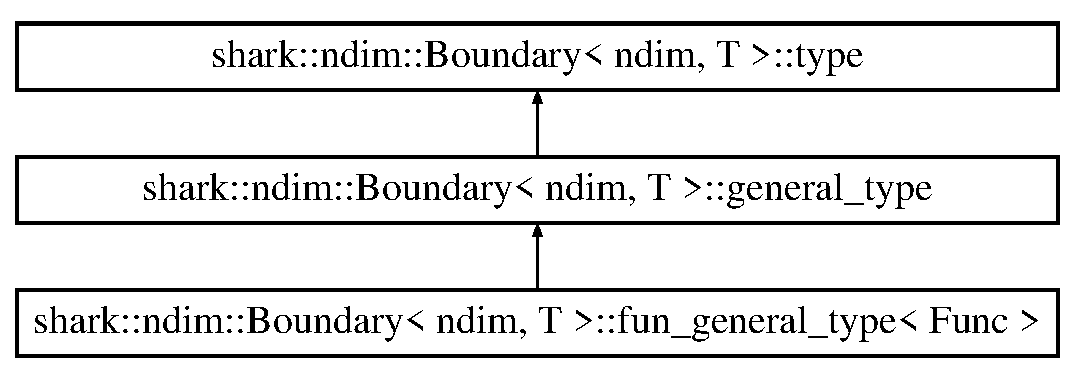
\includegraphics[height=3.000000cm]{classshark_1_1ndim_1_1_boundary_1_1general__type}
\end{center}
\end{figure}
\subsection*{Public Member Functions}
\begin{DoxyCompactItemize}
\item 
virtual void \hyperlink{classshark_1_1ndim_1_1_boundary_1_1general__type_ac73340187c707591d7fc1ccbe85c1b19}{set} (\hyperlink{classshark_1_1ndim_1_1_access}{Access}$<$ ndim, T $>$ \&a, \hyperlink{structshark_1_1ndim_1_1coords__range}{coords\+\_\+range}$<$ ndim $>$ r, long k) const =0
\end{DoxyCompactItemize}


\subsection{Detailed Description}
\subsubsection*{template$<$int ndim, typename T$>$\newline
class shark\+::ndim\+::\+Boundary$<$ ndim, T $>$\+::general\+\_\+type}



Definition at line 47 of file boundary.\+hpp.



\subsection{Member Function Documentation}
\hypertarget{classshark_1_1ndim_1_1_boundary_1_1general__type_ac73340187c707591d7fc1ccbe85c1b19}{}\label{classshark_1_1ndim_1_1_boundary_1_1general__type_ac73340187c707591d7fc1ccbe85c1b19} 
\index{shark\+::ndim\+::\+Boundary\+::general\+\_\+type@{shark\+::ndim\+::\+Boundary\+::general\+\_\+type}!set@{set}}
\index{set@{set}!shark\+::ndim\+::\+Boundary\+::general\+\_\+type@{shark\+::ndim\+::\+Boundary\+::general\+\_\+type}}
\subsubsection{\texorpdfstring{set()}{set()}}
{\footnotesize\ttfamily template$<$int ndim, typename T$>$ \\
virtual void \hyperlink{classshark_1_1ndim_1_1_boundary}{shark\+::ndim\+::\+Boundary}$<$ ndim, T $>$\+::general\+\_\+type\+::set (\begin{DoxyParamCaption}\item[{\hyperlink{classshark_1_1ndim_1_1_access}{Access}$<$ ndim, T $>$ \&}]{a,  }\item[{\hyperlink{structshark_1_1ndim_1_1coords__range}{coords\+\_\+range}$<$ ndim $>$}]{r,  }\item[{long}]{k }\end{DoxyParamCaption}) const\hspace{0.3cm}{\ttfamily [pure virtual]}}



Implemented in \hyperlink{classshark_1_1ndim_1_1_boundary_1_1fun__general__type_a7f5d89a026065de5a42b757ce507a70f}{shark\+::ndim\+::\+Boundary$<$ ndim, T $>$\+::fun\+\_\+general\+\_\+type$<$ Func $>$}.



The documentation for this class was generated from the following file\+:\begin{DoxyCompactItemize}
\item 
include/shark/\hyperlink{boundary_8hpp}{boundary.\+hpp}\end{DoxyCompactItemize}

\hypertarget{classshark_1_1ndim_1_1_global_array}{}\section{shark\+:\+:ndim\+:\+:Global\+Array$<$ ndim, T $>$ Class Template Reference}
\label{classshark_1_1ndim_1_1_global_array}\index{shark\+::ndim\+::\+Global\+Array$<$ ndim, T $>$@{shark\+::ndim\+::\+Global\+Array$<$ ndim, T $>$}}


{\ttfamily \#include $<$common.\+hpp$>$}

\subsection*{Public Types}
\begin{DoxyCompactItemize}
\item 
typedef T \hyperlink{classshark_1_1ndim_1_1_global_array_ac2471050153d015a155f4c7106ae5b7c}{value\+\_\+type}
\item 
typedef \hyperlink{classshark_1_1ndim_1_1_g_a_ref}{G\+A\+Ref}$<$ ndim, T $>$ \hyperlink{classshark_1_1ndim_1_1_global_array_a776d645cf4cd4ca129af3b082d139936}{storage}
\item 
typedef \hyperlink{classshark_1_1ndim_1_1_access}{Access}$<$ ndim, T $>$ \hyperlink{classshark_1_1ndim_1_1_global_array_ac19db430fee866f14a2d8f64aabec734}{accessor}
\item 
typedef std\+::array$<$ \hyperlink{classshark_1_1ndim_1_1_boundary}{Boundary}$<$ ndim, T $>$, ndim $>$ \hyperlink{classshark_1_1ndim_1_1_global_array_a5376df376a8de6a0a756def884c55864}{bounds}
\end{DoxyCompactItemize}
\subsection*{Public Member Functions}
\begin{DoxyCompactItemize}
\item 
\hyperlink{common_8hpp_a2eb6f9e0395b47b8d5e3eeae4fe0c116}{I\+N\+L\+I\+NE} T \& \hyperlink{classshark_1_1ndim_1_1_global_array_aeadb9a62b97953c4b7a7a047632d117a}{da} (\hyperlink{structshark_1_1ndim_1_1coords}{coords}$<$ ndim $>$ i) const
\item 
\hyperlink{common_8hpp_a2eb6f9e0395b47b8d5e3eeae4fe0c116}{I\+N\+L\+I\+NE} T $\ast$ \hyperlink{classshark_1_1ndim_1_1_global_array_a31a8a5247cc8adbe0602a83de759d915}{pa} (\hyperlink{structshark_1_1ndim_1_1coords}{coords}$<$ ndim $>$ i) const
\item 
\hyperlink{common_8hpp_a2eb6f9e0395b47b8d5e3eeae4fe0c116}{I\+N\+L\+I\+NE} \hyperlink{namespaceshark_a767a92d5dd82cb82266473bff42fa6d9}{coord} \hyperlink{classshark_1_1ndim_1_1_global_array_a63c8f10949e3f8d7ffdf532440190ca1}{offset} (\hyperlink{structshark_1_1ndim_1_1coords}{coords}$<$ ndim $>$ i) const
\item 
\hyperlink{common_8hpp_a2eb6f9e0395b47b8d5e3eeae4fe0c116}{I\+N\+L\+I\+NE} \hyperlink{namespaceshark_a767a92d5dd82cb82266473bff42fa6d9}{coord} \hyperlink{classshark_1_1ndim_1_1_global_array_afc41f124baff4e53c97c38c8cbd82398}{byte\+\_\+offset} (\hyperlink{structshark_1_1ndim_1_1coords}{coords}$<$ ndim $>$ i) const
\item 
std\+::ostream \& \hyperlink{classshark_1_1ndim_1_1_global_array_ae56b93f4ac19003102749015275a6d0c}{log\+\_\+out} () const
\item 
\hyperlink{common_8hpp_a2eb6f9e0395b47b8d5e3eeae4fe0c116}{I\+N\+L\+I\+NE} const \hyperlink{classshark_1_1ndim_1_1_domain}{Domain}$<$ ndim $>$ \& \hyperlink{classshark_1_1ndim_1_1_global_array_a435ee8ff23c3feadf2ef2be64d4f375c}{domain} () const
\item 
\hyperlink{common_8hpp_a2eb6f9e0395b47b8d5e3eeae4fe0c116}{I\+N\+L\+I\+NE} \hyperlink{structshark_1_1ndim_1_1coords}{coords}$<$ ndim $>$ \hyperlink{classshark_1_1ndim_1_1_global_array_a5331f21887f3c14791b758e99656a676}{ghost\+\_\+width} () const
\item 
\hyperlink{common_8hpp_a2eb6f9e0395b47b8d5e3eeae4fe0c116}{I\+N\+L\+I\+NE} bool \hyperlink{classshark_1_1ndim_1_1_global_array_abf0c9312657087578f89e1279ee6c451}{ghost\+\_\+corners} () const
\item 
\hyperlink{common_8hpp_a2eb6f9e0395b47b8d5e3eeae4fe0c116}{I\+N\+L\+I\+NE} \hyperlink{classshark_1_1ndim_1_1_global_array_aca73ba70ecbbc7f3224fd48582a15447}{operator bool} () const
\item 
\hyperlink{common_8hpp_a2eb6f9e0395b47b8d5e3eeae4fe0c116}{I\+N\+L\+I\+NE} \hyperlink{structshark_1_1ndim_1_1coords__range}{coords\+\_\+range}$<$ ndim $>$ \hyperlink{classshark_1_1ndim_1_1_global_array_a40939e7384b55a49b59c63dc717224d2}{region} () const
\item 
\hyperlink{common_8hpp_a2eb6f9e0395b47b8d5e3eeae4fe0c116}{I\+N\+L\+I\+NE} \hyperlink{structshark_1_1ndim_1_1coords__range}{coords\+\_\+range}$<$ ndim $>$ \hyperlink{classshark_1_1ndim_1_1_global_array_a871fb1acbd9bd46439766121053e20d1}{local} () const
\item 
\hyperlink{common_8hpp_a2eb6f9e0395b47b8d5e3eeae4fe0c116}{I\+N\+L\+I\+NE} \hyperlink{structshark_1_1ndim_1_1coords__range}{coords\+\_\+range}$<$ ndim $>$ \hyperlink{classshark_1_1ndim_1_1_global_array_a9bba546920e1709b492540d4ef0b0129}{inner} () const
\item 
\hyperlink{common_8hpp_a2eb6f9e0395b47b8d5e3eeae4fe0c116}{I\+N\+L\+I\+NE} \hyperlink{structshark_1_1ndim_1_1coords__range}{coords\+\_\+range}$<$ ndim $>$ \hyperlink{classshark_1_1ndim_1_1_global_array_a991cfff5cda18b938bc52cfc1c383680}{outer\+\_\+front} (int) const
\item 
\hyperlink{common_8hpp_a2eb6f9e0395b47b8d5e3eeae4fe0c116}{I\+N\+L\+I\+NE} \hyperlink{structshark_1_1ndim_1_1coords__range}{coords\+\_\+range}$<$ ndim $>$ \hyperlink{classshark_1_1ndim_1_1_global_array_a6f07daf32776f286cffa8620a456a3cd}{outer\+\_\+back} (int) const
\item 
\hyperlink{common_8hpp_a2eb6f9e0395b47b8d5e3eeae4fe0c116}{I\+N\+L\+I\+NE} std\+::vector$<$ \hyperlink{structshark_1_1ndim_1_1coords__range}{coords\+\_\+range}$<$ ndim $>$ $>$ \hyperlink{classshark_1_1ndim_1_1_global_array_a93f43e778ca040cb2ca8ad05dcb02ab0}{outer} () const
\item 
\hyperlink{common_8hpp_a2eb6f9e0395b47b8d5e3eeae4fe0c116}{I\+N\+L\+I\+NE} std\+::vector$<$ \hyperlink{structshark_1_1ndim_1_1coords__range}{coords\+\_\+range}$<$ ndim $>$ $>$ \hyperlink{classshark_1_1ndim_1_1_global_array_a9c72fd2f409389cb47a6f47bdfb77582}{split} (\hyperlink{structshark_1_1ndim_1_1coords__range}{coords\+\_\+range}$<$ ndim $>$) const
\item 
\hyperlink{common_8hpp_a2eb6f9e0395b47b8d5e3eeae4fe0c116}{I\+N\+L\+I\+NE} \hyperlink{structshark_1_1ndim_1_1coords__range}{coords\+\_\+range}$<$ ndim $>$ \hyperlink{classshark_1_1ndim_1_1_global_array_a8432959070aee7062f09cae8e7f20097}{ghost\+\_\+in\+\_\+front} (int) const
\item 
\hyperlink{common_8hpp_a2eb6f9e0395b47b8d5e3eeae4fe0c116}{I\+N\+L\+I\+NE} \hyperlink{structshark_1_1ndim_1_1coords__range}{coords\+\_\+range}$<$ ndim $>$ \hyperlink{classshark_1_1ndim_1_1_global_array_a55074d9d00de584f5817668e0c69f58a}{ghost\+\_\+in\+\_\+back} (int) const
\item 
\hyperlink{common_8hpp_a2eb6f9e0395b47b8d5e3eeae4fe0c116}{I\+N\+L\+I\+NE} \hyperlink{structshark_1_1ndim_1_1coords__range}{coords\+\_\+range}$<$ ndim $>$ \hyperlink{classshark_1_1ndim_1_1_global_array_ad004cd3a0deeaee55d7f3590063d5a20}{ghost\+\_\+out\+\_\+front} (int) const
\item 
\hyperlink{common_8hpp_a2eb6f9e0395b47b8d5e3eeae4fe0c116}{I\+N\+L\+I\+NE} \hyperlink{structshark_1_1ndim_1_1coords__range}{coords\+\_\+range}$<$ ndim $>$ \hyperlink{classshark_1_1ndim_1_1_global_array_ae4618013580af820c76c7e48d6de874a}{ghost\+\_\+out\+\_\+back} (int) const
\item 
\hyperlink{classshark_1_1ndim_1_1_g_a_dest}{G\+A\+Dest}$<$ ndim, T $>$ \hyperlink{classshark_1_1ndim_1_1_global_array_aab2d58e37ec78fd0aca6a6366e9b7aac}{region} (\hyperlink{structshark_1_1ndim_1_1coords__range}{coords\+\_\+range}$<$ ndim $>$, bool=true)
\item 
\hyperlink{classshark_1_1ndim_1_1_global_array_a5ab08686e28785763adac3fa73673f84}{Global\+Array} ()
\item 
\hyperlink{classshark_1_1ndim_1_1_global_array_aa1fb3bab347e8bc9c1347f46c2e3e4dd}{Global\+Array} (const \hyperlink{classshark_1_1ndim_1_1_domain}{Domain}$<$ ndim $>$ \&\hyperlink{classshark_1_1ndim_1_1_global_array_a435ee8ff23c3feadf2ef2be64d4f375c}{domain}, \hyperlink{structshark_1_1ndim_1_1coords}{coords}$<$ ndim $>$ \hyperlink{classshark_1_1ndim_1_1_global_array_a5331f21887f3c14791b758e99656a676}{ghost\+\_\+width}=\hyperlink{structshark_1_1ndim_1_1coords}{coords}$<$ ndim $>$(), bool \hyperlink{classshark_1_1ndim_1_1_global_array_abf0c9312657087578f89e1279ee6c451}{ghost\+\_\+corners}=false, \hyperlink{classshark_1_1ndim_1_1_global_array_a5376df376a8de6a0a756def884c55864}{bounds} \hyperlink{classshark_1_1ndim_1_1_global_array_aead89700a3d1d960432c6dc971251a9c}{bd}=\hyperlink{classshark_1_1ndim_1_1_global_array_a5376df376a8de6a0a756def884c55864}{bounds}())
\item 
\hyperlink{classshark_1_1ndim_1_1_global_array_a97e27f44095bf15566679fbb45377e2f}{Global\+Array} (const \hyperlink{classshark_1_1ndim_1_1_global_array}{Global\+Array}$<$ ndim, T $>$ \&other, bool copy)
\item 
\hyperlink{classshark_1_1ndim_1_1_global_array_acd71722990795db5e20aefc9e5545add}{$\sim$\+Global\+Array} ()
\item 
\hyperlink{classshark_1_1ndim_1_1_global_array_ac2140f54377695ea7d2898ebfe69fee9}{Global\+Array} (const \hyperlink{classshark_1_1ndim_1_1_global_array}{Global\+Array}$<$ ndim, T $>$ \&other)=delete
\item 
\hyperlink{classshark_1_1ndim_1_1_global_array_a963ccb19d6e77904259a7ca500cfb514}{Global\+Array} (\hyperlink{classshark_1_1ndim_1_1_global_array}{Global\+Array}$<$ ndim, T $>$ \&\&other)
\item 
\hyperlink{classshark_1_1ndim_1_1_global_array}{Global\+Array}$<$ ndim, T $>$ \& \hyperlink{classshark_1_1ndim_1_1_global_array_a65fd825eff8e4b3d49f1111e487991f3}{operator=} (\hyperlink{classshark_1_1ndim_1_1_global_array}{Global\+Array}$<$ ndim, T $>$ \&\&other)
\item 
\hyperlink{classshark_1_1ndim_1_1_global_array}{Global\+Array}$<$ ndim, T $>$ \& \hyperlink{classshark_1_1ndim_1_1_global_array_a34d08c80663eaade55f75682e3c12e2f}{operator=} (const \hyperlink{classshark_1_1ndim_1_1_global_array}{Global\+Array}$<$ ndim, T $>$ \&other)
\item 
{\footnotesize template$<$typename S $>$ }\\\hyperlink{classshark_1_1ndim_1_1_global_array}{Global\+Array}$<$ ndim, T $>$ \& \hyperlink{classshark_1_1ndim_1_1_global_array_a4a66a7ee10a7ba6c22690c74824ce73e}{operator=} (const S \&)
\item 
{\footnotesize template$<$typename S $>$ }\\\hyperlink{classshark_1_1ndim_1_1_global_array}{Global\+Array}$<$ ndim, T $>$ \& \hyperlink{classshark_1_1ndim_1_1_global_array_ab76900c34fa648d9a953fbfb55c5131e}{operator$<$$<$=} (const S \&)
\item 
void \hyperlink{classshark_1_1ndim_1_1_global_array_a27631077480a0cda76b968d6b21f0da4}{update} (long k=0) const
\begin{DoxyCompactList}\small\item\em 

 \end{DoxyCompactList}\item 
\hyperlink{structshark_1_1_future}{Future}$<$ void $>$ \hyperlink{classshark_1_1ndim_1_1_global_array_a6485a70dbb541c3bc600fb96903169ef}{iupdate} (long k=0) const
\item 
void \hyperlink{classshark_1_1ndim_1_1_global_array_ac7949ae0526bc0a8ca3b7a3561a3b788}{get} (\hyperlink{structshark_1_1ndim_1_1coords__range}{coords\+\_\+range}$<$ ndim $>$ range\+\_\+src, \hyperlink{classshark_1_1ndim_1_1_global_array}{Global\+Array}$<$ ndim, T $>$ \&src, \hyperlink{structshark_1_1ndim_1_1coords__range}{coords\+\_\+range}$<$ ndim $>$ range\+\_\+tgt)
\item 
void \hyperlink{classshark_1_1ndim_1_1_global_array_a655f6da8e7f336f63669a0008f324e36}{get} (\hyperlink{structshark_1_1ndim_1_1coords__range}{coords\+\_\+range}$<$ ndim $>$ range, T $\ast$buf) const
\item 
void \hyperlink{classshark_1_1ndim_1_1_global_array_a7df181f976618d26c70d6a2b364ab459}{get} (\hyperlink{structshark_1_1ndim_1_1coords__range}{coords\+\_\+range}$<$ ndim $>$ range, std\+::array$<$ std\+::size\+\_\+t, ndim-\/1 $>$ \hyperlink{classshark_1_1ndim_1_1_global_array_afdc4665e0fde4a703785436af351df49}{ld}, T $\ast$buf) const
\item 
void \hyperlink{classshark_1_1ndim_1_1_global_array_a243017e228365f73049fdb7136bb40a6}{put} (\hyperlink{structshark_1_1ndim_1_1coords__range}{coords\+\_\+range}$<$ ndim $>$ range\+\_\+tgt, \hyperlink{classshark_1_1ndim_1_1_global_array}{Global\+Array}$<$ ndim, T $>$ \&src, \hyperlink{structshark_1_1ndim_1_1coords__range}{coords\+\_\+range}$<$ ndim $>$ range\+\_\+src)
\item 
void \hyperlink{classshark_1_1ndim_1_1_global_array_a068b9c1fc5d00815b8be060454e14d6d}{put} (\hyperlink{structshark_1_1ndim_1_1coords__range}{coords\+\_\+range}$<$ ndim $>$ range, const T $\ast$buf)
\item 
void \hyperlink{classshark_1_1ndim_1_1_global_array_a078514cc8388c3c48964b958d2ff5dc7}{put} (\hyperlink{structshark_1_1ndim_1_1coords__range}{coords\+\_\+range}$<$ ndim $>$ range, std\+::array$<$ std\+::size\+\_\+t, ndim-\/1 $>$ \hyperlink{classshark_1_1ndim_1_1_global_array_afdc4665e0fde4a703785436af351df49}{ld}, const T $\ast$buf)
\item 
void \hyperlink{classshark_1_1ndim_1_1_global_array_a56bc7c60d0516eedcdc4be9c88bdba11}{accumulate} (\hyperlink{structshark_1_1ndim_1_1coords__range}{coords\+\_\+range}$<$ ndim $>$ range\+\_\+tgt, \hyperlink{classshark_1_1ndim_1_1_global_array}{Global\+Array}$<$ ndim, T $>$ \&src, \hyperlink{structshark_1_1ndim_1_1coords__range}{coords\+\_\+range}$<$ ndim $>$ range\+\_\+src)
\item 
{\footnotesize template$<$typename  = void$>$ }\\void \hyperlink{classshark_1_1ndim_1_1_global_array_a2afde2694e3e5a09dc1f782b5f0f3b82}{dump} (\hyperlink{structshark_1_1ndim_1_1coords__range}{coords\+\_\+range}$<$ ndim $>$ range, std\+::string filename)
\end{DoxyCompactItemize}
\subsection*{Public Attributes}
\begin{DoxyCompactItemize}
\item 
T $\ast$ \hyperlink{classshark_1_1ndim_1_1_global_array_ad4af3b8307a3a7107186cf699b5a2432}{ptr}
\item 
std\+::unique\+\_\+ptr$<$ \hyperlink{classshark_1_1ndim_1_1_g_a_impl}{G\+A\+Impl}$<$ ndim, T $>$ $>$ \hyperlink{classshark_1_1ndim_1_1_global_array_a70684121da4badfef791c15d7076282f}{impl}
\item 
std\+::array$<$ \hyperlink{classshark_1_1ndim_1_1_g_a_buf}{G\+A\+Buf}$<$ ndim, T $>$, ndim $>$ \hyperlink{classshark_1_1ndim_1_1_global_array_a1f7c189d498d7e7c1c79d9a613d1c5a9}{g\+\_\+out\+\_\+back}
\item 
std\+::array$<$ \hyperlink{classshark_1_1ndim_1_1_g_a_buf}{G\+A\+Buf}$<$ ndim, T $>$, ndim $>$ \hyperlink{classshark_1_1ndim_1_1_global_array_ad811cd36846992d5671148e7da49bb04}{g\+\_\+out\+\_\+front}
\item 
std\+::array$<$ \hyperlink{classshark_1_1ndim_1_1_g_a_buf}{G\+A\+Buf}$<$ ndim, T $>$, ndim $>$ \hyperlink{classshark_1_1ndim_1_1_global_array_a148e8382e63e8ff0c9fece28f1131702}{g\+\_\+in\+\_\+back}
\item 
std\+::array$<$ \hyperlink{classshark_1_1ndim_1_1_g_a_buf}{G\+A\+Buf}$<$ ndim, T $>$, ndim $>$ \hyperlink{classshark_1_1ndim_1_1_global_array_a2f3fe48d925bc0c3a489b83203eaddfe}{g\+\_\+in\+\_\+front}
\end{DoxyCompactItemize}
\subsection*{Static Public Attributes}
\begin{DoxyCompactItemize}
\item 
static const int \hyperlink{classshark_1_1ndim_1_1_global_array_aa97c2cc7bef528fca0118cac8e8a5c39}{number\+\_\+of\+\_\+dimensions} = ndim
\end{DoxyCompactItemize}
\subsection*{Private Member Functions}
\begin{DoxyCompactItemize}
\item 
void \hyperlink{classshark_1_1ndim_1_1_global_array_ad7054741564c962156640415d208dc72}{allocate} ()
\item 
void \hyperlink{classshark_1_1ndim_1_1_global_array_a62353dca76c53cee5fb9cfa5f31cd542}{deallocate} ()
\item 
void \hyperlink{classshark_1_1ndim_1_1_global_array_a8f1fa6f1d6408a1b34b35a50bf551733}{reset} ()
\end{DoxyCompactItemize}
\subsection*{Private Attributes}
\begin{DoxyCompactItemize}
\item 
const \hyperlink{classshark_1_1ndim_1_1_domain}{Domain}$<$ ndim $>$ $\ast$ \hyperlink{classshark_1_1ndim_1_1_global_array_a412e192f4c7a15888da625ae833e8d3e}{dom}
\item 
\hyperlink{structshark_1_1ndim_1_1coords}{coords}$<$ ndim $>$ \hyperlink{classshark_1_1ndim_1_1_global_array_a38d93d114d585e5e5491c5ecd35c6bfc}{gw}
\item 
bool \hyperlink{classshark_1_1ndim_1_1_global_array_a100f4d523420deffde330079df7501e2}{gc}
\item 
\hyperlink{classshark_1_1ndim_1_1_global_array_a5376df376a8de6a0a756def884c55864}{bounds} \hyperlink{classshark_1_1ndim_1_1_global_array_aead89700a3d1d960432c6dc971251a9c}{bd}
\item 
\hyperlink{structshark_1_1ndim_1_1coords}{coords}$<$ ndim+1 $>$ \hyperlink{classshark_1_1ndim_1_1_global_array_afdc4665e0fde4a703785436af351df49}{ld}
\item 
std\+::array$<$ \hyperlink{structshark_1_1ndim_1_1coords__range}{coords\+\_\+range}$<$ ndim $>$, ndim $>$ \hyperlink{classshark_1_1ndim_1_1_global_array_a97eb47a8cd80d98627706e673259a310}{ghost\+\_\+back}
\item 
std\+::array$<$ \hyperlink{structshark_1_1ndim_1_1coords__range}{coords\+\_\+range}$<$ ndim $>$, ndim $>$ \hyperlink{classshark_1_1ndim_1_1_global_array_a48ce861293f294f003ef16ebd49eb942}{ghost\+\_\+front}
\item 
int \hyperlink{classshark_1_1ndim_1_1_global_array_a8248f4bd6e1f48d25148dd6d5288cb4c}{lc}
\end{DoxyCompactItemize}
\subsection*{Friends}
\begin{DoxyCompactItemize}
\item 
class \hyperlink{classshark_1_1ndim_1_1_global_array_aa496c51f4f4225904ad62cb63601e053}{Access$<$ ndim, T $>$}
\item 
void \hyperlink{classshark_1_1ndim_1_1_global_array_a2f0f1152d3993384631952178a21f82e}{get} (\hyperlink{classshark_1_1ndim_1_1_global_array}{Global\+Array}$<$ ndim, T $>$ \&tgt, \hyperlink{structshark_1_1ndim_1_1coords__range}{coords\+\_\+range}$<$ ndim $>$ range\+\_\+src, \hyperlink{classshark_1_1ndim_1_1_global_array}{Global\+Array}$<$ ndim, T $>$ \&src, \hyperlink{structshark_1_1ndim_1_1coords__range}{coords\+\_\+range}$<$ ndim $>$ range\+\_\+tgt)
\item 
void \hyperlink{classshark_1_1ndim_1_1_global_array_ad96ea2c2b281921d915e7a8834420f06}{put} (\hyperlink{classshark_1_1ndim_1_1_global_array}{Global\+Array}$<$ ndim, T $>$ \&tgt, \hyperlink{structshark_1_1ndim_1_1coords__range}{coords\+\_\+range}$<$ ndim $>$ range\+\_\+src, \hyperlink{classshark_1_1ndim_1_1_global_array}{Global\+Array}$<$ ndim, T $>$ \&src, \hyperlink{structshark_1_1ndim_1_1coords__range}{coords\+\_\+range}$<$ ndim $>$ range\+\_\+tgt)
\item 
void \hyperlink{classshark_1_1ndim_1_1_global_array_aa95eda1df3e42435fbeddc71a7bebeb9}{accumulate} (\hyperlink{classshark_1_1ndim_1_1_global_array}{Global\+Array}$<$ ndim, T $>$ \&tgt, \hyperlink{structshark_1_1ndim_1_1coords__range}{coords\+\_\+range}$<$ ndim $>$ range\+\_\+src, \hyperlink{classshark_1_1ndim_1_1_global_array}{Global\+Array}$<$ ndim, T $>$ \&src, \hyperlink{structshark_1_1ndim_1_1coords__range}{coords\+\_\+range}$<$ ndim $>$ range\+\_\+tgt)
\end{DoxyCompactItemize}


\subsection{Detailed Description}
\subsubsection*{template$<$int ndim, typename T$>$\newline
class shark\+::ndim\+::\+Global\+Array$<$ ndim, T $>$}

A global array that is partitioned across a process group according to a domain 

Definition at line 167 of file common.\+hpp.



\subsection{Member Typedef Documentation}
\hypertarget{classshark_1_1ndim_1_1_global_array_ac19db430fee866f14a2d8f64aabec734}{}\label{classshark_1_1ndim_1_1_global_array_ac19db430fee866f14a2d8f64aabec734} 
\index{shark\+::ndim\+::\+Global\+Array@{shark\+::ndim\+::\+Global\+Array}!accessor@{accessor}}
\index{accessor@{accessor}!shark\+::ndim\+::\+Global\+Array@{shark\+::ndim\+::\+Global\+Array}}
\subsubsection{\texorpdfstring{accessor}{accessor}}
{\footnotesize\ttfamily template$<$int ndim, typename T$>$ \\
typedef \hyperlink{classshark_1_1ndim_1_1_access}{Access}$<$ndim,T$>$ \hyperlink{classshark_1_1ndim_1_1_global_array}{shark\+::ndim\+::\+Global\+Array}$<$ ndim, T $>$\+::\hyperlink{classshark_1_1ndim_1_1_global_array_ac19db430fee866f14a2d8f64aabec734}{accessor}}



Definition at line 59 of file globalarray.\+hpp.

\hypertarget{classshark_1_1ndim_1_1_global_array_a5376df376a8de6a0a756def884c55864}{}\label{classshark_1_1ndim_1_1_global_array_a5376df376a8de6a0a756def884c55864} 
\index{shark\+::ndim\+::\+Global\+Array@{shark\+::ndim\+::\+Global\+Array}!bounds@{bounds}}
\index{bounds@{bounds}!shark\+::ndim\+::\+Global\+Array@{shark\+::ndim\+::\+Global\+Array}}
\subsubsection{\texorpdfstring{bounds}{bounds}}
{\footnotesize\ttfamily template$<$int ndim, typename T$>$ \\
typedef std\+::array$<$\hyperlink{classshark_1_1ndim_1_1_boundary}{Boundary}$<$ndim,T$>$,ndim$>$ \hyperlink{classshark_1_1ndim_1_1_global_array}{shark\+::ndim\+::\+Global\+Array}$<$ ndim, T $>$\+::\hyperlink{classshark_1_1ndim_1_1_global_array_a5376df376a8de6a0a756def884c55864}{bounds}}



Definition at line 61 of file globalarray.\+hpp.

\hypertarget{classshark_1_1ndim_1_1_global_array_a776d645cf4cd4ca129af3b082d139936}{}\label{classshark_1_1ndim_1_1_global_array_a776d645cf4cd4ca129af3b082d139936} 
\index{shark\+::ndim\+::\+Global\+Array@{shark\+::ndim\+::\+Global\+Array}!storage@{storage}}
\index{storage@{storage}!shark\+::ndim\+::\+Global\+Array@{shark\+::ndim\+::\+Global\+Array}}
\subsubsection{\texorpdfstring{storage}{storage}}
{\footnotesize\ttfamily template$<$int ndim, typename T$>$ \\
typedef \hyperlink{classshark_1_1ndim_1_1_g_a_ref}{G\+A\+Ref}$<$ndim,T$>$ \hyperlink{classshark_1_1ndim_1_1_global_array}{shark\+::ndim\+::\+Global\+Array}$<$ ndim, T $>$\+::\hyperlink{classshark_1_1ndim_1_1_global_array_a776d645cf4cd4ca129af3b082d139936}{storage}}



Definition at line 58 of file globalarray.\+hpp.

\hypertarget{classshark_1_1ndim_1_1_global_array_ac2471050153d015a155f4c7106ae5b7c}{}\label{classshark_1_1ndim_1_1_global_array_ac2471050153d015a155f4c7106ae5b7c} 
\index{shark\+::ndim\+::\+Global\+Array@{shark\+::ndim\+::\+Global\+Array}!value\+\_\+type@{value\+\_\+type}}
\index{value\+\_\+type@{value\+\_\+type}!shark\+::ndim\+::\+Global\+Array@{shark\+::ndim\+::\+Global\+Array}}
\subsubsection{\texorpdfstring{value\+\_\+type}{value\_type}}
{\footnotesize\ttfamily template$<$int ndim, typename T$>$ \\
typedef T \hyperlink{classshark_1_1ndim_1_1_global_array}{shark\+::ndim\+::\+Global\+Array}$<$ ndim, T $>$\+::\hyperlink{classshark_1_1ndim_1_1_global_array_ac2471050153d015a155f4c7106ae5b7c}{value\+\_\+type}}



Definition at line 57 of file globalarray.\+hpp.



\subsection{Constructor \& Destructor Documentation}
\hypertarget{classshark_1_1ndim_1_1_global_array_a5ab08686e28785763adac3fa73673f84}{}\label{classshark_1_1ndim_1_1_global_array_a5ab08686e28785763adac3fa73673f84} 
\index{shark\+::ndim\+::\+Global\+Array@{shark\+::ndim\+::\+Global\+Array}!Global\+Array@{Global\+Array}}
\index{Global\+Array@{Global\+Array}!shark\+::ndim\+::\+Global\+Array@{shark\+::ndim\+::\+Global\+Array}}
\subsubsection{\texorpdfstring{Global\+Array()}{GlobalArray()}\hspace{0.1cm}{\footnotesize\ttfamily [1/5]}}
{\footnotesize\ttfamily template$<$int ndim, typename T $>$ \\
Global\+Array\+::\+Global\+Array (\begin{DoxyParamCaption}{ }\end{DoxyParamCaption})}

Construct a \hyperlink{classshark_1_1ndim_1_1_global_array}{Global\+Array} (collective). The global array will not be active until it is assigned. 

Definition at line 42 of file globalarray.\+cpp.


\begin{DoxyCode}
42 : \hyperlink{classshark_1_1ndim_1_1_global_array_a412e192f4c7a15888da625ae833e8d3e}{dom}(0) \{ \}
\end{DoxyCode}
\hypertarget{classshark_1_1ndim_1_1_global_array_aa1fb3bab347e8bc9c1347f46c2e3e4dd}{}\label{classshark_1_1ndim_1_1_global_array_aa1fb3bab347e8bc9c1347f46c2e3e4dd} 
\index{shark\+::ndim\+::\+Global\+Array@{shark\+::ndim\+::\+Global\+Array}!Global\+Array@{Global\+Array}}
\index{Global\+Array@{Global\+Array}!shark\+::ndim\+::\+Global\+Array@{shark\+::ndim\+::\+Global\+Array}}
\subsubsection{\texorpdfstring{Global\+Array()}{GlobalArray()}\hspace{0.1cm}{\footnotesize\ttfamily [2/5]}}
{\footnotesize\ttfamily template$<$int ndim, typename T $>$ \\
Global\+Array\+::\+Global\+Array (\begin{DoxyParamCaption}\item[{const \hyperlink{classshark_1_1ndim_1_1_domain}{Domain}$<$ ndim $>$ \&}]{domain,  }\item[{\hyperlink{structshark_1_1ndim_1_1coords}{coords}$<$ ndim $>$}]{ghost\+\_\+width = {\ttfamily \hyperlink{structshark_1_1ndim_1_1coords}{coords}$<$ndim$>$()},  }\item[{bool}]{ghost\+\_\+corners = {\ttfamily false},  }\item[{\hyperlink{classshark_1_1ndim_1_1_global_array_a5376df376a8de6a0a756def884c55864}{bounds}}]{bd = {\ttfamily \hyperlink{classshark_1_1ndim_1_1_global_array_a5376df376a8de6a0a756def884c55864}{bounds}()} }\end{DoxyParamCaption})}

Construct a \hyperlink{classshark_1_1ndim_1_1_global_array}{Global\+Array} (collective). 
\begin{DoxyParams}{Parameters}
{\em domain} & the domain for the distribution of data \\
\hline
{\em ghost\+\_\+width} & number of ghost cells for each dimension \\
\hline
{\em ghost\+\_\+corners} & whether to maintain the corner ghost cells \\
\hline
\end{DoxyParams}


Definition at line 245 of file globalarray.\+cpp.


\begin{DoxyCode}
245                                                                                                            
              :
246   \hyperlink{classshark_1_1ndim_1_1_global_array_a412e192f4c7a15888da625ae833e8d3e}{dom}(&domain), \hyperlink{classshark_1_1ndim_1_1_global_array_a38d93d114d585e5e5491c5ecd35c6bfc}{gw}(ghost\_width), \hyperlink{classshark_1_1ndim_1_1_global_array_a100f4d523420deffde330079df7501e2}{gc}(\hyperlink{classshark_1_1ndim_1_1_global_array_abf0c9312657087578f89e1279ee6c451}{ghost\_corners}), \hyperlink{classshark_1_1ndim_1_1_global_array_aead89700a3d1d960432c6dc971251a9c}{bd}(\hyperlink{classshark_1_1ndim_1_1_global_array_aead89700a3d1d960432c6dc971251a9c}{bd}), 
      \hyperlink{classshark_1_1ndim_1_1_global_array_a70684121da4badfef791c15d7076282f}{impl}(\textcolor{keyword}{new} \hyperlink{classshark_1_1ndim_1_1_g_a_impl}{GAImpl<ndim,T>}()), \hyperlink{classshark_1_1ndim_1_1_global_array_a8248f4bd6e1f48d25148dd6d5288cb4c}{lc}(0) \{
247     \hyperlink{classshark_1_1ndim_1_1_global_array_ad7054741564c962156640415d208dc72}{allocate}();
248 \}
\end{DoxyCode}
\hypertarget{classshark_1_1ndim_1_1_global_array_a97e27f44095bf15566679fbb45377e2f}{}\label{classshark_1_1ndim_1_1_global_array_a97e27f44095bf15566679fbb45377e2f} 
\index{shark\+::ndim\+::\+Global\+Array@{shark\+::ndim\+::\+Global\+Array}!Global\+Array@{Global\+Array}}
\index{Global\+Array@{Global\+Array}!shark\+::ndim\+::\+Global\+Array@{shark\+::ndim\+::\+Global\+Array}}
\subsubsection{\texorpdfstring{Global\+Array()}{GlobalArray()}\hspace{0.1cm}{\footnotesize\ttfamily [3/5]}}
{\footnotesize\ttfamily template$<$int ndim, typename T $>$ \\
Global\+Array\+::\+Global\+Array (\begin{DoxyParamCaption}\item[{const \hyperlink{classshark_1_1ndim_1_1_global_array}{Global\+Array}$<$ ndim, T $>$ \&}]{other,  }\item[{bool}]{copy }\end{DoxyParamCaption})}



Definition at line 251 of file globalarray.\+cpp.


\begin{DoxyCode}
251                                                                            :
252   \hyperlink{classshark_1_1ndim_1_1_global_array_a412e192f4c7a15888da625ae833e8d3e}{dom}(other.\hyperlink{classshark_1_1ndim_1_1_global_array_a412e192f4c7a15888da625ae833e8d3e}{dom}), \hyperlink{classshark_1_1ndim_1_1_global_array_a38d93d114d585e5e5491c5ecd35c6bfc}{gw}(other.\hyperlink{classshark_1_1ndim_1_1_global_array_a38d93d114d585e5e5491c5ecd35c6bfc}{gw}), \hyperlink{classshark_1_1ndim_1_1_global_array_a100f4d523420deffde330079df7501e2}{gc}(other.\hyperlink{classshark_1_1ndim_1_1_global_array_a100f4d523420deffde330079df7501e2}{gc}), \hyperlink{classshark_1_1ndim_1_1_global_array_aead89700a3d1d960432c6dc971251a9c}{bd}(other.\hyperlink{classshark_1_1ndim_1_1_global_array_aead89700a3d1d960432c6dc971251a9c}{bd}), 
      \hyperlink{classshark_1_1ndim_1_1_global_array_a70684121da4badfef791c15d7076282f}{impl}(\textcolor{keyword}{new} \hyperlink{classshark_1_1ndim_1_1_g_a_impl}{GAImpl<ndim,T>}()), \hyperlink{classshark_1_1ndim_1_1_global_array_a8248f4bd6e1f48d25148dd6d5288cb4c}{lc}(0) \{
253     \hyperlink{classshark_1_1ndim_1_1_global_array_ad7054741564c962156640415d208dc72}{allocate}();
254 
255     \textcolor{keywordflow}{if}(copy)
256         *\textcolor{keyword}{this} = other;
257 \}
\end{DoxyCode}
\hypertarget{classshark_1_1ndim_1_1_global_array_acd71722990795db5e20aefc9e5545add}{}\label{classshark_1_1ndim_1_1_global_array_acd71722990795db5e20aefc9e5545add} 
\index{shark\+::ndim\+::\+Global\+Array@{shark\+::ndim\+::\+Global\+Array}!````~Global\+Array@{$\sim$\+Global\+Array}}
\index{````~Global\+Array@{$\sim$\+Global\+Array}!shark\+::ndim\+::\+Global\+Array@{shark\+::ndim\+::\+Global\+Array}}
\subsubsection{\texorpdfstring{$\sim$\+Global\+Array()}{~GlobalArray()}}
{\footnotesize\ttfamily template$<$int ndim, typename T $>$ \\
Global\+Array\+::$\sim$\+Global\+Array (\begin{DoxyParamCaption}{ }\end{DoxyParamCaption})}

Destruct a \hyperlink{classshark_1_1ndim_1_1_global_array}{Global\+Array} (collective). If active, the memory of the global array is released 

Definition at line 45 of file globalarray.\+cpp.


\begin{DoxyCode}
46 \{
47     \textcolor{keywordflow}{if}(*\textcolor{keyword}{this})
48     \{
49         assert(\hyperlink{classshark_1_1ndim_1_1_global_array_a8248f4bd6e1f48d25148dd6d5288cb4c}{lc} == 0);
50         \hyperlink{classshark_1_1ndim_1_1_global_array_a62353dca76c53cee5fb9cfa5f31cd542}{deallocate}();
51     \}
52 \}
\end{DoxyCode}
\hypertarget{classshark_1_1ndim_1_1_global_array_ac2140f54377695ea7d2898ebfe69fee9}{}\label{classshark_1_1ndim_1_1_global_array_ac2140f54377695ea7d2898ebfe69fee9} 
\index{shark\+::ndim\+::\+Global\+Array@{shark\+::ndim\+::\+Global\+Array}!Global\+Array@{Global\+Array}}
\index{Global\+Array@{Global\+Array}!shark\+::ndim\+::\+Global\+Array@{shark\+::ndim\+::\+Global\+Array}}
\subsubsection{\texorpdfstring{Global\+Array()}{GlobalArray()}\hspace{0.1cm}{\footnotesize\ttfamily [4/5]}}
{\footnotesize\ttfamily template$<$int ndim, typename T$>$ \\
\hyperlink{classshark_1_1ndim_1_1_global_array}{shark\+::ndim\+::\+Global\+Array}$<$ ndim, T $>$\+::\hyperlink{classshark_1_1ndim_1_1_global_array}{Global\+Array} (\begin{DoxyParamCaption}\item[{const \hyperlink{classshark_1_1ndim_1_1_global_array}{Global\+Array}$<$ ndim, T $>$ \&}]{other }\end{DoxyParamCaption})\hspace{0.3cm}{\ttfamily [delete]}}

\hypertarget{classshark_1_1ndim_1_1_global_array_a963ccb19d6e77904259a7ca500cfb514}{}\label{classshark_1_1ndim_1_1_global_array_a963ccb19d6e77904259a7ca500cfb514} 
\index{shark\+::ndim\+::\+Global\+Array@{shark\+::ndim\+::\+Global\+Array}!Global\+Array@{Global\+Array}}
\index{Global\+Array@{Global\+Array}!shark\+::ndim\+::\+Global\+Array@{shark\+::ndim\+::\+Global\+Array}}
\subsubsection{\texorpdfstring{Global\+Array()}{GlobalArray()}\hspace{0.1cm}{\footnotesize\ttfamily [5/5]}}
{\footnotesize\ttfamily template$<$int ndim, typename T $>$ \\
Global\+Array\+::\+Global\+Array (\begin{DoxyParamCaption}\item[{\hyperlink{classshark_1_1ndim_1_1_global_array}{Global\+Array}$<$ ndim, T $>$ \&\&}]{other }\end{DoxyParamCaption})}



Definition at line 55 of file globalarray.\+cpp.


\begin{DoxyCode}
55                                                            :
56     \hyperlink{classshark_1_1ndim_1_1_global_array_a412e192f4c7a15888da625ae833e8d3e}{dom}(other.\hyperlink{classshark_1_1ndim_1_1_global_array_a412e192f4c7a15888da625ae833e8d3e}{dom}),
57     \hyperlink{classshark_1_1ndim_1_1_global_array_a38d93d114d585e5e5491c5ecd35c6bfc}{gw}(other.\hyperlink{classshark_1_1ndim_1_1_global_array_a38d93d114d585e5e5491c5ecd35c6bfc}{gw}),
58     \hyperlink{classshark_1_1ndim_1_1_global_array_a100f4d523420deffde330079df7501e2}{gc}(other.\hyperlink{classshark_1_1ndim_1_1_global_array_a100f4d523420deffde330079df7501e2}{gc}),
59     \hyperlink{classshark_1_1ndim_1_1_global_array_aead89700a3d1d960432c6dc971251a9c}{bd}(std::move(other.\hyperlink{classshark_1_1ndim_1_1_global_array_aead89700a3d1d960432c6dc971251a9c}{bd})),
60     \hyperlink{classshark_1_1ndim_1_1_global_array_ad4af3b8307a3a7107186cf699b5a2432}{ptr}(other.\hyperlink{classshark_1_1ndim_1_1_global_array_ad4af3b8307a3a7107186cf699b5a2432}{ptr}),
61     \hyperlink{classshark_1_1ndim_1_1_global_array_a70684121da4badfef791c15d7076282f}{impl}(std::move(other.\hyperlink{classshark_1_1ndim_1_1_global_array_a70684121da4badfef791c15d7076282f}{impl})),
62     \hyperlink{classshark_1_1ndim_1_1_global_array_afdc4665e0fde4a703785436af351df49}{ld}(std::move(other.\hyperlink{classshark_1_1ndim_1_1_global_array_afdc4665e0fde4a703785436af351df49}{ld})),
63     \hyperlink{classshark_1_1ndim_1_1_global_array_a97eb47a8cd80d98627706e673259a310}{ghost\_back}(std::move(other.\hyperlink{classshark_1_1ndim_1_1_global_array_a97eb47a8cd80d98627706e673259a310}{ghost\_back})),
64     \hyperlink{classshark_1_1ndim_1_1_global_array_a48ce861293f294f003ef16ebd49eb942}{ghost\_front}(std::move(other.\hyperlink{classshark_1_1ndim_1_1_global_array_a48ce861293f294f003ef16ebd49eb942}{ghost\_front})),
65     \hyperlink{classshark_1_1ndim_1_1_global_array_a8248f4bd6e1f48d25148dd6d5288cb4c}{lc}(0),
66     \hyperlink{classshark_1_1ndim_1_1_global_array_a1f7c189d498d7e7c1c79d9a613d1c5a9}{g\_out\_back}(std::move(other.\hyperlink{classshark_1_1ndim_1_1_global_array_a1f7c189d498d7e7c1c79d9a613d1c5a9}{g\_out\_back})),
67     \hyperlink{classshark_1_1ndim_1_1_global_array_ad811cd36846992d5671148e7da49bb04}{g\_out\_front}(std::move(other.\hyperlink{classshark_1_1ndim_1_1_global_array_ad811cd36846992d5671148e7da49bb04}{g\_out\_front})),
68     \hyperlink{classshark_1_1ndim_1_1_global_array_a148e8382e63e8ff0c9fece28f1131702}{g\_in\_back}(std::move(other.\hyperlink{classshark_1_1ndim_1_1_global_array_a148e8382e63e8ff0c9fece28f1131702}{g\_in\_back})),
69     \hyperlink{classshark_1_1ndim_1_1_global_array_a2f3fe48d925bc0c3a489b83203eaddfe}{g\_in\_front}(std::move(other.\hyperlink{classshark_1_1ndim_1_1_global_array_a2f3fe48d925bc0c3a489b83203eaddfe}{g\_in\_front}))
70 \{
71     assert(!other || other.\hyperlink{classshark_1_1ndim_1_1_global_array_a8248f4bd6e1f48d25148dd6d5288cb4c}{lc} == 0);
72     other.\hyperlink{classshark_1_1ndim_1_1_global_array_a8f1fa6f1d6408a1b34b35a50bf551733}{reset}();
73 \}
\end{DoxyCode}


\subsection{Member Function Documentation}
\hypertarget{classshark_1_1ndim_1_1_global_array_a56bc7c60d0516eedcdc4be9c88bdba11}{}\label{classshark_1_1ndim_1_1_global_array_a56bc7c60d0516eedcdc4be9c88bdba11} 
\index{shark\+::ndim\+::\+Global\+Array@{shark\+::ndim\+::\+Global\+Array}!accumulate@{accumulate}}
\index{accumulate@{accumulate}!shark\+::ndim\+::\+Global\+Array@{shark\+::ndim\+::\+Global\+Array}}
\subsubsection{\texorpdfstring{accumulate()}{accumulate()}}
{\footnotesize\ttfamily template$<$int ndim, typename T $>$ \\
void Global\+Array\+::accumulate (\begin{DoxyParamCaption}\item[{\hyperlink{structshark_1_1ndim_1_1coords__range}{coords\+\_\+range}$<$ ndim $>$}]{range\+\_\+tgt,  }\item[{\hyperlink{classshark_1_1ndim_1_1_global_array}{Global\+Array}$<$ ndim, T $>$ \&}]{src,  }\item[{\hyperlink{structshark_1_1ndim_1_1coords__range}{coords\+\_\+range}$<$ ndim $>$}]{range\+\_\+src }\end{DoxyParamCaption})}

Increase remote range with local values (one-\/sided). R\+MA operations cannot overlap with local access. 
\begin{DoxyParams}{Parameters}
{\em range} & the area of the global array to update \\
\hline
{\em ld} & the strides to use for buf (default\+: determined by range) \\
\hline
{\em buf} & the source buffer \\
\hline
\end{DoxyParams}


Definition at line 946 of file globalarray.\+cpp.


\begin{DoxyCode}
946                                                                                                            
                     \{
947     \hyperlink{namespaceshark_1_1ndim_ac2fdde52862b140ea3d88f43d31425fe}{shark::ndim::accumulate}(*\textcolor{keyword}{this}, range\_dst, src, range\_src);
948 \} 
\end{DoxyCode}
\hypertarget{classshark_1_1ndim_1_1_global_array_ad7054741564c962156640415d208dc72}{}\label{classshark_1_1ndim_1_1_global_array_ad7054741564c962156640415d208dc72} 
\index{shark\+::ndim\+::\+Global\+Array@{shark\+::ndim\+::\+Global\+Array}!allocate@{allocate}}
\index{allocate@{allocate}!shark\+::ndim\+::\+Global\+Array@{shark\+::ndim\+::\+Global\+Array}}
\subsubsection{\texorpdfstring{allocate()}{allocate()}}
{\footnotesize\ttfamily template$<$int ndim, typename T $>$ \\
void Global\+Array\+::allocate (\begin{DoxyParamCaption}{ }\end{DoxyParamCaption})\hspace{0.3cm}{\ttfamily [private]}}



Definition at line 111 of file globalarray.\+cpp.


\begin{DoxyCode}
112 \{
113     \textcolor{keyword}{const} \hyperlink{structshark_1_1ndim_1_1coords__range}{coords\_range<ndim>} \hyperlink{classshark_1_1ndim_1_1_global_array_a871fb1acbd9bd46439766121053e20d1}{local} = \hyperlink{classshark_1_1ndim_1_1_global_array_a435ee8ff23c3feadf2ef2be64d4f375c}{domain}().local();
114     \textcolor{keyword}{const} \hyperlink{structshark_1_1ndim_1_1coords}{coords<ndim>} \hyperlink{classshark_1_1ndim_1_1_global_array_a38d93d114d585e5e5491c5ecd35c6bfc}{gw} = \hyperlink{classshark_1_1ndim_1_1_global_array_a5331f21887f3c14791b758e99656a676}{ghost\_width}();
115     \textcolor{keyword}{const} \textcolor{keywordtype}{bool} \hyperlink{classshark_1_1ndim_1_1_global_array_a100f4d523420deffde330079df7501e2}{gc} = \hyperlink{classshark_1_1ndim_1_1_global_array_abf0c9312657087578f89e1279ee6c451}{ghost\_corners}(); 
116 
117     \textcolor{comment}{// Allocate memory}
118     \hyperlink{classshark_1_1ndim_1_1_global_array_afdc4665e0fde4a703785436af351df49}{ld} = local.stride(gw);
119         \textcolor{keywordtype}{unsigned} count = \hyperlink{classshark_1_1ndim_1_1_global_array_afdc4665e0fde4a703785436af351df49}{ld}[0];
120 
121     \textcolor{keywordflow}{for}(\textcolor{keywordtype}{int} di = 0; di < ndim; di++) \{
122         \textcolor{keywordflow}{for}(\textcolor{keywordtype}{int} d = 0; d < ndim; d++) \{
123 \textcolor{preprocessor}{#ifdef SHARK\_STPACK}
124                         \hyperlink{namespaceshark_a767a92d5dd82cb82266473bff42fa6d9}{coord} gw\_prev = gw[d];
125                         \hyperlink{namespaceshark_a767a92d5dd82cb82266473bff42fa6d9}{coord} gw\_next = gw[d];
126 \textcolor{preprocessor}{#else}
127                         \textcolor{keywordtype}{bool} pd = \textcolor{keyword}{dynamic\_cast<}typename 
      \hyperlink{classshark_1_1ndim_1_1_boundary_1_1periodic__type}{Boundary<ndim,T>::periodic\_type}*\textcolor{keyword}{>}(\hyperlink{classshark_1_1ndim_1_1_global_array_aead89700a3d1d960432c6dc971251a9c}{bd}[di].t.get()) != \textcolor{keyword}{nullptr};
128                         \textcolor{keywordtype}{int} prev = \hyperlink{classshark_1_1ndim_1_1_global_array_a435ee8ff23c3feadf2ef2be64d4f375c}{domain}().shiftd(di, -1, pd);
129                         \textcolor{keywordtype}{int} next = \hyperlink{classshark_1_1ndim_1_1_global_array_a435ee8ff23c3feadf2ef2be64d4f375c}{domain}().shiftd(di,  1, pd);
130                         \hyperlink{namespaceshark_a767a92d5dd82cb82266473bff42fa6d9}{coord} gw\_prev = prev < 0 ? 0 : gw[d];
131                         \hyperlink{namespaceshark_a767a92d5dd82cb82266473bff42fa6d9}{coord} gw\_next = next < 0 ? 0 : gw[d];
132 \textcolor{preprocessor}{#endif}
133 
134             \textcolor{keywordflow}{if}(d == di)
135             \{
136                 \hyperlink{classshark_1_1ndim_1_1_global_array_a97eb47a8cd80d98627706e673259a310}{ghost\_back} [di].lower[d] = local.\hyperlink{structshark_1_1ndim_1_1coords__range_a46cae2c424d7b20f911a970c92581b19}{lower}[d] - gw\_prev;
137                 \hyperlink{classshark_1_1ndim_1_1_global_array_a97eb47a8cd80d98627706e673259a310}{ghost\_back} [di].upper[d] = local.\hyperlink{structshark_1_1ndim_1_1coords__range_a46cae2c424d7b20f911a970c92581b19}{lower}[d];
138                 \hyperlink{classshark_1_1ndim_1_1_global_array_a48ce861293f294f003ef16ebd49eb942}{ghost\_front}[di].lower[d] = local.\hyperlink{structshark_1_1ndim_1_1coords__range_ae0101e4bb3ecadf1faa0fc786dfb05db}{upper}[d];
139                 \hyperlink{classshark_1_1ndim_1_1_global_array_a48ce861293f294f003ef16ebd49eb942}{ghost\_front}[di].upper[d] = local.\hyperlink{structshark_1_1ndim_1_1coords__range_ae0101e4bb3ecadf1faa0fc786dfb05db}{upper}[d] + gw\_next;
140             \}
141             \textcolor{keywordflow}{else} \textcolor{keywordflow}{if}(gc && d < di)
142             \{
143                 \hyperlink{classshark_1_1ndim_1_1_global_array_a97eb47a8cd80d98627706e673259a310}{ghost\_back} [di].lower[d] = local.\hyperlink{structshark_1_1ndim_1_1coords__range_a46cae2c424d7b20f911a970c92581b19}{lower}[d] - gw\_prev;
144                 \hyperlink{classshark_1_1ndim_1_1_global_array_a97eb47a8cd80d98627706e673259a310}{ghost\_back} [di].upper[d] = local.\hyperlink{structshark_1_1ndim_1_1coords__range_ae0101e4bb3ecadf1faa0fc786dfb05db}{upper}[d] + gw\_prev;
145                 \hyperlink{classshark_1_1ndim_1_1_global_array_a48ce861293f294f003ef16ebd49eb942}{ghost\_front}[di].lower[d] = local.\hyperlink{structshark_1_1ndim_1_1coords__range_a46cae2c424d7b20f911a970c92581b19}{lower}[d] - gw\_next;
146                 \hyperlink{classshark_1_1ndim_1_1_global_array_a48ce861293f294f003ef16ebd49eb942}{ghost\_front}[di].upper[d] = local.\hyperlink{structshark_1_1ndim_1_1coords__range_ae0101e4bb3ecadf1faa0fc786dfb05db}{upper}[d] + gw\_next;
147             \}
148             \textcolor{keywordflow}{else}
149             \{
150                 \hyperlink{classshark_1_1ndim_1_1_global_array_a97eb47a8cd80d98627706e673259a310}{ghost\_back} [di].lower[d] = local.\hyperlink{structshark_1_1ndim_1_1coords__range_a46cae2c424d7b20f911a970c92581b19}{lower}[d];
151                 \hyperlink{classshark_1_1ndim_1_1_global_array_a97eb47a8cd80d98627706e673259a310}{ghost\_back} [di].upper[d] = local.\hyperlink{structshark_1_1ndim_1_1coords__range_ae0101e4bb3ecadf1faa0fc786dfb05db}{upper}[d];
152                 \hyperlink{classshark_1_1ndim_1_1_global_array_a48ce861293f294f003ef16ebd49eb942}{ghost\_front}[di].lower[d] = local.\hyperlink{structshark_1_1ndim_1_1coords__range_a46cae2c424d7b20f911a970c92581b19}{lower}[d];
153                 \hyperlink{classshark_1_1ndim_1_1_global_array_a48ce861293f294f003ef16ebd49eb942}{ghost\_front}[di].upper[d] = local.\hyperlink{structshark_1_1ndim_1_1coords__range_ae0101e4bb3ecadf1faa0fc786dfb05db}{upper}[d];
154             \}
155                 \}
156 
157                 count += 2* \hyperlink{classshark_1_1ndim_1_1_global_array_a97eb47a8cd80d98627706e673259a310}{ghost\_back}[di].count();
158                 count += 2* \hyperlink{classshark_1_1ndim_1_1_global_array_a48ce861293f294f003ef16ebd49eb942}{ghost\_front}[di].count();
159         \}
160 
161     \textcolor{keywordtype}{unsigned} size = count * \textcolor{keyword}{sizeof}(T);
162 
163 \textcolor{preprocessor}{#ifndef NDEBUG}
164     \textcolor{keywordflow}{if}(\hyperlink{namespaceshark_a110e03e8104b06caef346fcc25621aa9}{log\_mask}[\hyperlink{namespaceshark_a067e8941bdd5f38f5ab2e49920787b9d}{verbose\_alloc}])
165         \hyperlink{classshark_1_1ndim_1_1_global_array_ae56b93f4ac19003102749015275a6d0c}{log\_out}() << \textcolor{stringliteral}{"allocate "} << local << endl;
166 \textcolor{preprocessor}{#endif}
167 \textcolor{preprocessor}{#if defined(SHARK\_MPI\_COMM) || defined(SHARK\_GPI\_COMM)}
168     \{
169         \textcolor{comment}{// Create ghost types}
170         MPI\_Datatype base = mpi\_type<T>::t;
171         \textcolor{keywordflow}{if}(mpi\_type<T>::count() != 1)
172             MPI\_Type\_contiguous(mpi\_type<T>::count(), base, &base);
173         MPI\_Aint lb, extent;
174         MPI\_Type\_get\_extent(base, &lb, &extent);
175 
176         \textcolor{keywordflow}{for}(\textcolor{keywordtype}{int} di = 0; di < ndim; di++)
177         \{
178             MPI\_Type\_dup(base, &\hyperlink{classshark_1_1ndim_1_1_global_array_a70684121da4badfef791c15d7076282f}{impl}->ghost[di]);
179 
180             \textcolor{keywordflow}{for}(\textcolor{keywordtype}{int} d = ndim-1; d >= 0; d--)
181             \{
182                 MPI\_Datatype tmp = \hyperlink{classshark_1_1ndim_1_1_global_array_a70684121da4badfef791c15d7076282f}{impl}->ghost[di];
183                 \hyperlink{namespaceshark_a767a92d5dd82cb82266473bff42fa6d9}{coord} n = \hyperlink{classshark_1_1ndim_1_1_global_array_a97eb47a8cd80d98627706e673259a310}{ghost\_back}[di].upper[d] - \hyperlink{classshark_1_1ndim_1_1_global_array_a97eb47a8cd80d98627706e673259a310}{ghost\_back}[di].lower[d];
184                 MPI\_Type\_create\_hvector(n, 1, \hyperlink{classshark_1_1ndim_1_1_global_array_afdc4665e0fde4a703785436af351df49}{ld}[d+1]*extent, tmp, &\hyperlink{classshark_1_1ndim_1_1_global_array_a70684121da4badfef791c15d7076282f}{impl}->ghost[di]);
185                 MPI\_Type\_free(&tmp);
186             \}
187 
188             MPI\_Type\_commit(&\hyperlink{classshark_1_1ndim_1_1_global_array_a70684121da4badfef791c15d7076282f}{impl}->ghost[di]);
189         \}
190 
191         \textcolor{keywordflow}{if}(mpi\_type<T>::count() != 1)
192             MPI\_Type\_free(&base);
193     \}
194 
195 
196 \textcolor{preprocessor}{#if defined(SHARK\_GPI\_COMM)}
197         \hyperlink{classshark_1_1ndim_1_1_global_array_a70684121da4badfef791c15d7076282f}{impl}->seg = GroupImpl::next\_seg\_id();
198         success\_or\_die(gaspi\_segment\_create(\hyperlink{classshark_1_1ndim_1_1_global_array_a70684121da4badfef791c15d7076282f}{impl}->seg, size, \hyperlink{classshark_1_1ndim_1_1_global_array_a435ee8ff23c3feadf2ef2be64d4f375c}{domain}().group.impl->grp, 
      GASPI\_BLOCK, GASPI\_ALLOC\_DEFAULT));  
199         gaspi\_segment\_ptr(\hyperlink{classshark_1_1ndim_1_1_global_array_a70684121da4badfef791c15d7076282f}{impl}->seg, (gaspi\_pointer\_t*)&\hyperlink{classshark_1_1ndim_1_1_global_array_ad4af3b8307a3a7107186cf699b5a2432}{ptr});
200         assert(\hyperlink{classshark_1_1ndim_1_1_global_array_ad4af3b8307a3a7107186cf699b5a2432}{ptr});
201 \textcolor{preprocessor}{#else}
202     MPI\_Alloc\_mem(size, MPI\_INFO\_NULL, &\hyperlink{classshark_1_1ndim_1_1_global_array_ad4af3b8307a3a7107186cf699b5a2432}{ptr});
203 \textcolor{preprocessor}{#endif}
204 
205     \textcolor{comment}{// Create window}
206     MPI\_Win\_create(\hyperlink{classshark_1_1ndim_1_1_global_array_ad4af3b8307a3a7107186cf699b5a2432}{ptr}, size, static\_cast<int>(\textcolor{keyword}{sizeof}(T)), MPI\_INFO\_NULL, 
      \hyperlink{classshark_1_1ndim_1_1_global_array_a435ee8ff23c3feadf2ef2be64d4f375c}{domain}().group.impl->comm, &\hyperlink{classshark_1_1ndim_1_1_global_array_a70684121da4badfef791c15d7076282f}{impl}->win);
207 \textcolor{preprocessor}{#elif defined(SHARK\_NO\_COMM)}
208     unused(\hyperlink{classshark_1_1ndim_1_1_global_array_a70684121da4badfef791c15d7076282f}{impl});
209     \hyperlink{classshark_1_1ndim_1_1_global_array_ad4af3b8307a3a7107186cf699b5a2432}{ptr} = \textcolor{keyword}{static\_cast<}T*\textcolor{keyword}{>}(mem\_alloc(size));
210 \textcolor{preprocessor}{#else}
211 \textcolor{preprocessor}{#error "No comm allocate"}
212 \textcolor{preprocessor}{#endif}
213 
214     \{
215         \textcolor{keyword}{typename} \hyperlink{classshark_1_1ndim_1_1_domain_a9684ccd8af33cff7639c782290ac37ee}{Domain<ndim>::pcoords} np = \hyperlink{classshark_1_1ndim_1_1_global_array_a435ee8ff23c3feadf2ef2be64d4f375c}{domain}().np;
216         \textcolor{keyword}{typename} \hyperlink{classshark_1_1ndim_1_1_domain_a9684ccd8af33cff7639c782290ac37ee}{Domain<ndim>::pcoords} ip = \hyperlink{classshark_1_1ndim_1_1_global_array_a435ee8ff23c3feadf2ef2be64d4f375c}{domain}().indexp();
217         \hyperlink{classshark_1_1ndim_1_1_access}{Access<ndim,T>} acc(*\textcolor{keyword}{this});
218 
219         \textcolor{keywordflow}{for}(\textcolor{keywordtype}{int} di = 0; di < ndim; di++)
220                 \{
221                     \textcolor{keyword}{typename} \hyperlink{classshark_1_1ndim_1_1_boundary_1_1fixed__type}{Boundary<ndim,T>::fixed\_type}* b = \textcolor{keyword}{dynamic\_cast<}
      typename \hyperlink{classshark_1_1ndim_1_1_boundary_1_1fixed__type}{Boundary<ndim,T>::fixed\_type}*\textcolor{keyword}{>}(\hyperlink{classshark_1_1ndim_1_1_global_array_aead89700a3d1d960432c6dc971251a9c}{bd}[di].t.get());
222 
223                     \textcolor{keywordflow}{if}(b == \textcolor{keyword}{nullptr}) \textcolor{keywordflow}{continue};
224                     \textcolor{keywordflow}{if}(ip[di] == 0) b->\hyperlink{classshark_1_1ndim_1_1_boundary_1_1fixed__type_ad94ec2994049c5107d0ea5d24bf8cff3}{set}(acc, \hyperlink{classshark_1_1ndim_1_1_global_array_a97eb47a8cd80d98627706e673259a310}{ghost\_back}[di]);
225                     \textcolor{keywordflow}{if}(ip[di] == np[di]-1) b->\hyperlink{classshark_1_1ndim_1_1_boundary_1_1fixed__type_ad94ec2994049c5107d0ea5d24bf8cff3}{set}(acc, \hyperlink{classshark_1_1ndim_1_1_global_array_a48ce861293f294f003ef16ebd49eb942}{ghost\_front}[di]);
226                 \}
227     \}
228 
229         \textcolor{keyword}{auto} p = \hyperlink{classshark_1_1ndim_1_1_global_array_ad4af3b8307a3a7107186cf699b5a2432}{ptr} + \hyperlink{classshark_1_1ndim_1_1_global_array_afdc4665e0fde4a703785436af351df49}{ld}[0];
230     \textcolor{keywordflow}{for}(\textcolor{keywordtype}{int} di = 0; di < ndim; di++) \{
231                 \hyperlink{classshark_1_1ndim_1_1_global_array_a148e8382e63e8ff0c9fece28f1131702}{g\_in\_back}  [di] = \hyperlink{classshark_1_1ndim_1_1_g_a_buf}{GABuf<ndim,T>}(
      \hyperlink{classshark_1_1ndim_1_1_global_array_a55074d9d00de584f5817668e0c69f58a}{ghost\_in\_back}(di), p); 
232                 p += \hyperlink{classshark_1_1ndim_1_1_global_array_a55074d9d00de584f5817668e0c69f58a}{ghost\_in\_back}(di).count();
233                 \hyperlink{classshark_1_1ndim_1_1_global_array_a2f3fe48d925bc0c3a489b83203eaddfe}{g\_in\_front} [di] = \hyperlink{classshark_1_1ndim_1_1_g_a_buf}{GABuf<ndim,T>}(
      \hyperlink{classshark_1_1ndim_1_1_global_array_a8432959070aee7062f09cae8e7f20097}{ghost\_in\_front}(di), p);
234                 p += \hyperlink{classshark_1_1ndim_1_1_global_array_a8432959070aee7062f09cae8e7f20097}{ghost\_in\_front}(di).count();
235                 \hyperlink{classshark_1_1ndim_1_1_global_array_a1f7c189d498d7e7c1c79d9a613d1c5a9}{g\_out\_back} [di] = \hyperlink{classshark_1_1ndim_1_1_g_a_buf}{GABuf<ndim,T>}(
      \hyperlink{classshark_1_1ndim_1_1_global_array_ae4618013580af820c76c7e48d6de874a}{ghost\_out\_back}(di), p);
236                 p += \hyperlink{classshark_1_1ndim_1_1_global_array_ae4618013580af820c76c7e48d6de874a}{ghost\_out\_back}(di).count();
237                 \hyperlink{classshark_1_1ndim_1_1_global_array_ad811cd36846992d5671148e7da49bb04}{g\_out\_front}[di] = \hyperlink{classshark_1_1ndim_1_1_g_a_buf}{GABuf<ndim,T>}(
      \hyperlink{classshark_1_1ndim_1_1_global_array_ad004cd3a0deeaee55d7f3590063d5a20}{ghost\_out\_front}(di), p);
238                 p += \hyperlink{classshark_1_1ndim_1_1_global_array_ad004cd3a0deeaee55d7f3590063d5a20}{ghost\_out\_front}(di).count();
239         \}
240         assert(p == \hyperlink{classshark_1_1ndim_1_1_global_array_ad4af3b8307a3a7107186cf699b5a2432}{ptr} + count);
241 \}
\end{DoxyCode}
\hypertarget{classshark_1_1ndim_1_1_global_array_afc41f124baff4e53c97c38c8cbd82398}{}\label{classshark_1_1ndim_1_1_global_array_afc41f124baff4e53c97c38c8cbd82398} 
\index{shark\+::ndim\+::\+Global\+Array@{shark\+::ndim\+::\+Global\+Array}!byte\+\_\+offset@{byte\+\_\+offset}}
\index{byte\+\_\+offset@{byte\+\_\+offset}!shark\+::ndim\+::\+Global\+Array@{shark\+::ndim\+::\+Global\+Array}}
\subsubsection{\texorpdfstring{byte\+\_\+offset()}{byte\_offset()}}
{\footnotesize\ttfamily template$<$int ndim, typename T $>$ \\
\hyperlink{namespaceshark_a767a92d5dd82cb82266473bff42fa6d9}{coord} \hyperlink{classshark_1_1ndim_1_1_global_array}{shark\+::ndim\+::\+Global\+Array}$<$ ndim, T $>$\+::byte\+\_\+offset (\begin{DoxyParamCaption}\item[{\hyperlink{structshark_1_1ndim_1_1coords}{coords}$<$ ndim $>$}]{i }\end{DoxyParamCaption}) const\hspace{0.3cm}{\ttfamily [inline]}}



Definition at line 400 of file globalarray.\+hpp.


\begin{DoxyCode}
400                                                                           \{
401             \textcolor{keywordflow}{return} \hyperlink{classshark_1_1ndim_1_1_global_array_a63c8f10949e3f8d7ffdf532440190ca1}{offset}(i) * \textcolor{keyword}{sizeof}(T);
402         \}
\end{DoxyCode}
\hypertarget{classshark_1_1ndim_1_1_global_array_aeadb9a62b97953c4b7a7a047632d117a}{}\label{classshark_1_1ndim_1_1_global_array_aeadb9a62b97953c4b7a7a047632d117a} 
\index{shark\+::ndim\+::\+Global\+Array@{shark\+::ndim\+::\+Global\+Array}!da@{da}}
\index{da@{da}!shark\+::ndim\+::\+Global\+Array@{shark\+::ndim\+::\+Global\+Array}}
\subsubsection{\texorpdfstring{da()}{da()}}
{\footnotesize\ttfamily template$<$int ndim, typename T $>$ \\
T \& \hyperlink{classshark_1_1ndim_1_1_global_array}{shark\+::ndim\+::\+Global\+Array}$<$ ndim, T $>$\+::da (\begin{DoxyParamCaption}\item[{\hyperlink{structshark_1_1ndim_1_1coords}{coords}$<$ ndim $>$}]{i }\end{DoxyParamCaption}) const\hspace{0.3cm}{\ttfamily [inline]}}



Definition at line 390 of file globalarray.\+hpp.


\begin{DoxyCode}
390                                                               \{
391             \textcolor{keywordflow}{return} \hyperlink{classshark_1_1ndim_1_1_global_array_ad4af3b8307a3a7107186cf699b5a2432}{ptr}[\hyperlink{classshark_1_1ndim_1_1_global_array_a63c8f10949e3f8d7ffdf532440190ca1}{offset}(i)];
392         \}
\end{DoxyCode}
\hypertarget{classshark_1_1ndim_1_1_global_array_a62353dca76c53cee5fb9cfa5f31cd542}{}\label{classshark_1_1ndim_1_1_global_array_a62353dca76c53cee5fb9cfa5f31cd542} 
\index{shark\+::ndim\+::\+Global\+Array@{shark\+::ndim\+::\+Global\+Array}!deallocate@{deallocate}}
\index{deallocate@{deallocate}!shark\+::ndim\+::\+Global\+Array@{shark\+::ndim\+::\+Global\+Array}}
\subsubsection{\texorpdfstring{deallocate()}{deallocate()}}
{\footnotesize\ttfamily template$<$int ndim, typename T $>$ \\
void Global\+Array\+::deallocate (\begin{DoxyParamCaption}{ }\end{DoxyParamCaption})\hspace{0.3cm}{\ttfamily [private]}}



Definition at line 262 of file globalarray.\+cpp.


\begin{DoxyCode}
263 \{
264 \textcolor{preprocessor}{#if defined(SHARK\_MPI\_COMM)}
265     \textcolor{keywordflow}{for}(\textcolor{keywordtype}{int} di = 0; di < ndim; di++)
266         MPI\_Type\_free(&\hyperlink{classshark_1_1ndim_1_1_global_array_a70684121da4badfef791c15d7076282f}{impl}->ghost[di]);
267 
268     MPI\_Win\_free(&\hyperlink{classshark_1_1ndim_1_1_global_array_a70684121da4badfef791c15d7076282f}{impl}->win);
269     MPI\_Free\_mem(\hyperlink{classshark_1_1ndim_1_1_global_array_ad4af3b8307a3a7107186cf699b5a2432}{ptr});
270 \textcolor{preprocessor}{#elif defined(SHARK\_GPI\_COMM)}
271     gaspi\_segment\_delete(\hyperlink{classshark_1_1ndim_1_1_global_array_a70684121da4badfef791c15d7076282f}{impl}->seg);
272         GroupImpl::free\_seg\_id(\hyperlink{classshark_1_1ndim_1_1_global_array_a70684121da4badfef791c15d7076282f}{impl}->seg);
273 \textcolor{preprocessor}{#elif defined(SHARK\_NO\_COMM)}
274     mem\_free(\hyperlink{classshark_1_1ndim_1_1_global_array_ad4af3b8307a3a7107186cf699b5a2432}{ptr});
275 \textcolor{preprocessor}{#else}
276 \textcolor{preprocessor}{#error "No comm deallocate"}
277 \textcolor{preprocessor}{#endif}
278 \}
\end{DoxyCode}
\hypertarget{classshark_1_1ndim_1_1_global_array_a435ee8ff23c3feadf2ef2be64d4f375c}{}\label{classshark_1_1ndim_1_1_global_array_a435ee8ff23c3feadf2ef2be64d4f375c} 
\index{shark\+::ndim\+::\+Global\+Array@{shark\+::ndim\+::\+Global\+Array}!domain@{domain}}
\index{domain@{domain}!shark\+::ndim\+::\+Global\+Array@{shark\+::ndim\+::\+Global\+Array}}
\subsubsection{\texorpdfstring{domain()}{domain()}}
{\footnotesize\ttfamily template$<$int ndim, typename T $>$ \\
const \hyperlink{classshark_1_1ndim_1_1_domain}{Domain}$<$ ndim $>$ \& \hyperlink{classshark_1_1ndim_1_1_global_array}{shark\+::ndim\+::\+Global\+Array}$<$ ndim, T $>$\+::domain (\begin{DoxyParamCaption}{ }\end{DoxyParamCaption}) const\hspace{0.3cm}{\ttfamily [inline]}}

The domain 

Definition at line 273 of file globalarray.\+hpp.


\begin{DoxyCode}
273                                                                      \{
274             \textcolor{keywordflow}{return} *\hyperlink{classshark_1_1ndim_1_1_global_array_a412e192f4c7a15888da625ae833e8d3e}{dom};
275         \}
\end{DoxyCode}
\hypertarget{classshark_1_1ndim_1_1_global_array_a2afde2694e3e5a09dc1f782b5f0f3b82}{}\label{classshark_1_1ndim_1_1_global_array_a2afde2694e3e5a09dc1f782b5f0f3b82} 
\index{shark\+::ndim\+::\+Global\+Array@{shark\+::ndim\+::\+Global\+Array}!dump@{dump}}
\index{dump@{dump}!shark\+::ndim\+::\+Global\+Array@{shark\+::ndim\+::\+Global\+Array}}
\subsubsection{\texorpdfstring{dump()}{dump()}}
{\footnotesize\ttfamily template$<$int ndim, typename T $>$ \\
template$<$typename $>$ \\
void Global\+Array\+::dump (\begin{DoxyParamCaption}\item[{\hyperlink{structshark_1_1ndim_1_1coords__range}{coords\+\_\+range}$<$ ndim $>$}]{range,  }\item[{std\+::string}]{filename }\end{DoxyParamCaption})}

Dump values of global array to a file 

Definition at line 951 of file globalarray.\+cpp.


\begin{DoxyCode}
951                                                                            \{
952 \textcolor{preprocessor}{#ifndef NDEBUG}
953         \textcolor{keywordflow}{if}(\hyperlink{namespaceshark_a110e03e8104b06caef346fcc25621aa9}{log\_mask}[\hyperlink{namespaceshark_a8faafcaa495b6cf0c0eca37a846e45f2}{verbose\_rma}])
954                 this->\hyperlink{classshark_1_1ndim_1_1_global_array_ae56b93f4ac19003102749015275a6d0c}{log\_out}() << \textcolor{stringliteral}{"dump to "} << filename << endl;
955 \textcolor{preprocessor}{#endif}
956 \textcolor{preprocessor}{#if defined(SHARK\_MPI\_COMM) || defined(SHARK\_GPI\_COMM)}
957         MPI\_File fh;
958         MPI\_File\_open(MPI\_COMM\_WORLD, const\_cast<char*>(filename.c\_str()), MPI\_MODE\_CREATE | MPI\_MODE\_RDWR,
       MPI\_INFO\_NULL, &fh);
959 
960         \textcolor{comment}{// type for part to read from}
961         \hyperlink{structshark_1_1ndim_1_1coords__range}{coords\_range<ndim>} src = \hyperlink{classshark_1_1ndim_1_1_global_array_a435ee8ff23c3feadf2ef2be64d4f375c}{domain}().local().overlap(range);
962         \hyperlink{structshark_1_1ndim_1_1coords}{coords<ndim+1>} srcld = src.stride(\hyperlink{classshark_1_1ndim_1_1_global_array_a38d93d114d585e5e5491c5ecd35c6bfc}{gw});
963         \textcolor{keyword}{const} T* buf = \hyperlink{classshark_1_1ndim_1_1_global_array_a31a8a5247cc8adbe0602a83de759d915}{pa}(src.\hyperlink{structshark_1_1ndim_1_1coords__range_a46cae2c424d7b20f911a970c92581b19}{lower});
964         mpi\_type\_block<ndim,T> srct(src.counts(), srcld);
965         
966         \textcolor{comment}{// where to write to}
967         \hyperlink{structshark_1_1ndim_1_1coords__range}{coords\_range<ndim>} dst = \hyperlink{classshark_1_1ndim_1_1_global_array_a40939e7384b55a49b59c63dc717224d2}{region}().overlap(range);
968         \hyperlink{structshark_1_1ndim_1_1coords}{coords<ndim+1>} dstld = dst.stride(); \textcolor{comment}{// no ghost regions in file}
969         \hyperlink{namespaceshark_a767a92d5dd82cb82266473bff42fa6d9}{coord} dstoff = dst.lower.\hyperlink{structshark_1_1ndim_1_1coords_a0c905dc9ae7a2ea1c3a8cd4aaf542d73}{offset}(dstld); \textcolor{comment}{// offset wrt to global array}
970         
971         MPI\_File\_write\_at(fh, dstoff, const\_cast<T*>(buf), 1, srct.t, MPI\_STATUS\_IGNORE);
972 
973         MPI\_File\_close(&fh);
974 \textcolor{preprocessor}{#elif defined(SHARK\_NO\_COMM)}
975         FILE *fd = fopen(filename.c\_str(), \textcolor{stringliteral}{"w"});
976         \hyperlink{classshark_1_1ndim_1_1_access}{Access<ndim,T>} acc(*\textcolor{keyword}{this});
977     range.for\_each([&acc,fd](\hyperlink{structshark_1_1ndim_1_1coords}{coords<ndim>} ii) \{
978                 fwrite(&acc(ii), \textcolor{keyword}{sizeof}(T), 1, fd);
979     \});
980         fclose(fd);
981 \textcolor{preprocessor}{#else}
982 \textcolor{preprocessor}{#error "No comm dump"}
983 \textcolor{preprocessor}{#endif}
984 \}
\end{DoxyCode}
\hypertarget{classshark_1_1ndim_1_1_global_array_ac7949ae0526bc0a8ca3b7a3561a3b788}{}\label{classshark_1_1ndim_1_1_global_array_ac7949ae0526bc0a8ca3b7a3561a3b788} 
\index{shark\+::ndim\+::\+Global\+Array@{shark\+::ndim\+::\+Global\+Array}!get@{get}}
\index{get@{get}!shark\+::ndim\+::\+Global\+Array@{shark\+::ndim\+::\+Global\+Array}}
\subsubsection{\texorpdfstring{get()}{get()}\hspace{0.1cm}{\footnotesize\ttfamily [1/3]}}
{\footnotesize\ttfamily template$<$int ndim, typename T $>$ \\
void Global\+Array\+::get (\begin{DoxyParamCaption}\item[{\hyperlink{structshark_1_1ndim_1_1coords__range}{coords\+\_\+range}$<$ ndim $>$}]{range\+\_\+src,  }\item[{\hyperlink{classshark_1_1ndim_1_1_global_array}{Global\+Array}$<$ ndim, T $>$ \&}]{src,  }\item[{\hyperlink{structshark_1_1ndim_1_1coords__range}{coords\+\_\+range}$<$ ndim $>$}]{range\+\_\+tgt }\end{DoxyParamCaption})}

Get remote range (one-\/sided). R\+MA operations cannot overlap with local access. 
\begin{DoxyParams}{Parameters}
{\em range} & the area of the global array to retrieve from \\
\hline
{\em ld} & the strides to use for buf (default\+: determined by range) \\
\hline
{\em buf} & the target buffer \\
\hline
\end{DoxyParams}


Definition at line 787 of file globalarray.\+cpp.


\begin{DoxyCode}
787                                                                                                            
              \{
788     \textcolor{keyword}{auto} &src = *\textcolor{keyword}{this};
789     \hyperlink{namespaceshark_1_1ndim_a8a52bf045ab40d975bd382067a266ee8}{shark::ndim::get}(dst, range\_src, src, range\_dst);
790 \}
\end{DoxyCode}
\hypertarget{classshark_1_1ndim_1_1_global_array_a655f6da8e7f336f63669a0008f324e36}{}\label{classshark_1_1ndim_1_1_global_array_a655f6da8e7f336f63669a0008f324e36} 
\index{shark\+::ndim\+::\+Global\+Array@{shark\+::ndim\+::\+Global\+Array}!get@{get}}
\index{get@{get}!shark\+::ndim\+::\+Global\+Array@{shark\+::ndim\+::\+Global\+Array}}
\subsubsection{\texorpdfstring{get()}{get()}\hspace{0.1cm}{\footnotesize\ttfamily [2/3]}}
{\footnotesize\ttfamily template$<$int ndim, typename T $>$ \\
void Global\+Array\+::get (\begin{DoxyParamCaption}\item[{\hyperlink{structshark_1_1ndim_1_1coords__range}{coords\+\_\+range}$<$ ndim $>$}]{range,  }\item[{T $\ast$}]{buf }\end{DoxyParamCaption}) const}



Definition at line 684 of file globalarray.\+cpp.


\begin{DoxyCode}
684                                                                     \{
685     \textcolor{keyword}{get}(range, essential\_lead<ndim>(range.stride()), buf);
686 \}
\end{DoxyCode}
\hypertarget{classshark_1_1ndim_1_1_global_array_a7df181f976618d26c70d6a2b364ab459}{}\label{classshark_1_1ndim_1_1_global_array_a7df181f976618d26c70d6a2b364ab459} 
\index{shark\+::ndim\+::\+Global\+Array@{shark\+::ndim\+::\+Global\+Array}!get@{get}}
\index{get@{get}!shark\+::ndim\+::\+Global\+Array@{shark\+::ndim\+::\+Global\+Array}}
\subsubsection{\texorpdfstring{get()}{get()}\hspace{0.1cm}{\footnotesize\ttfamily [3/3]}}
{\footnotesize\ttfamily template$<$int ndim, typename T$>$ \\
void \hyperlink{classshark_1_1ndim_1_1_global_array}{shark\+::ndim\+::\+Global\+Array}$<$ ndim, T $>$\+::get (\begin{DoxyParamCaption}\item[{\hyperlink{structshark_1_1ndim_1_1coords__range}{coords\+\_\+range}$<$ ndim $>$}]{range,  }\item[{std\+::array$<$ std\+::size\+\_\+t, ndim-\/1 $>$}]{ld,  }\item[{T $\ast$}]{buf }\end{DoxyParamCaption}) const}

\hypertarget{classshark_1_1ndim_1_1_global_array_abf0c9312657087578f89e1279ee6c451}{}\label{classshark_1_1ndim_1_1_global_array_abf0c9312657087578f89e1279ee6c451} 
\index{shark\+::ndim\+::\+Global\+Array@{shark\+::ndim\+::\+Global\+Array}!ghost\+\_\+corners@{ghost\+\_\+corners}}
\index{ghost\+\_\+corners@{ghost\+\_\+corners}!shark\+::ndim\+::\+Global\+Array@{shark\+::ndim\+::\+Global\+Array}}
\subsubsection{\texorpdfstring{ghost\+\_\+corners()}{ghost\_corners()}}
{\footnotesize\ttfamily template$<$int ndim, typename T $>$ \\
bool \hyperlink{classshark_1_1ndim_1_1_global_array}{shark\+::ndim\+::\+Global\+Array}$<$ ndim, T $>$\+::ghost\+\_\+corners (\begin{DoxyParamCaption}{ }\end{DoxyParamCaption}) const\hspace{0.3cm}{\ttfamily [inline]}}

Whether corner ghost cells are maintained. 

Definition at line 283 of file globalarray.\+hpp.


\begin{DoxyCode}
283                                                              \{
284             \textcolor{keywordflow}{return} \hyperlink{classshark_1_1ndim_1_1_global_array_a100f4d523420deffde330079df7501e2}{gc};
285         \}
\end{DoxyCode}
\hypertarget{classshark_1_1ndim_1_1_global_array_a55074d9d00de584f5817668e0c69f58a}{}\label{classshark_1_1ndim_1_1_global_array_a55074d9d00de584f5817668e0c69f58a} 
\index{shark\+::ndim\+::\+Global\+Array@{shark\+::ndim\+::\+Global\+Array}!ghost\+\_\+in\+\_\+back@{ghost\+\_\+in\+\_\+back}}
\index{ghost\+\_\+in\+\_\+back@{ghost\+\_\+in\+\_\+back}!shark\+::ndim\+::\+Global\+Array@{shark\+::ndim\+::\+Global\+Array}}
\subsubsection{\texorpdfstring{ghost\+\_\+in\+\_\+back()}{ghost\_in\_back()}}
{\footnotesize\ttfamily template$<$int ndim, typename T $>$ \\
\hyperlink{structshark_1_1ndim_1_1coords__range}{coords\+\_\+range}$<$ ndim $>$ \hyperlink{classshark_1_1ndim_1_1_global_array}{shark\+::ndim\+::\+Global\+Array}$<$ ndim, T $>$\+::ghost\+\_\+in\+\_\+back (\begin{DoxyParamCaption}\item[{int}]{d }\end{DoxyParamCaption}) const\hspace{0.3cm}{\ttfamily [inline]}}



Definition at line 375 of file globalarray.\+hpp.


\begin{DoxyCode}
375                                                                                 \{
376                     \textcolor{keywordflow}{return} \hyperlink{classshark_1_1ndim_1_1_global_array_a97eb47a8cd80d98627706e673259a310}{ghost\_back}[d];
377                 \}
\end{DoxyCode}
\hypertarget{classshark_1_1ndim_1_1_global_array_a8432959070aee7062f09cae8e7f20097}{}\label{classshark_1_1ndim_1_1_global_array_a8432959070aee7062f09cae8e7f20097} 
\index{shark\+::ndim\+::\+Global\+Array@{shark\+::ndim\+::\+Global\+Array}!ghost\+\_\+in\+\_\+front@{ghost\+\_\+in\+\_\+front}}
\index{ghost\+\_\+in\+\_\+front@{ghost\+\_\+in\+\_\+front}!shark\+::ndim\+::\+Global\+Array@{shark\+::ndim\+::\+Global\+Array}}
\subsubsection{\texorpdfstring{ghost\+\_\+in\+\_\+front()}{ghost\_in\_front()}}
{\footnotesize\ttfamily template$<$int ndim, typename T $>$ \\
\hyperlink{structshark_1_1ndim_1_1coords__range}{coords\+\_\+range}$<$ ndim $>$ \hyperlink{classshark_1_1ndim_1_1_global_array}{shark\+::ndim\+::\+Global\+Array}$<$ ndim, T $>$\+::ghost\+\_\+in\+\_\+front (\begin{DoxyParamCaption}\item[{int}]{d }\end{DoxyParamCaption}) const\hspace{0.3cm}{\ttfamily [inline]}}



Definition at line 370 of file globalarray.\+hpp.


\begin{DoxyCode}
370                                                                                  \{
371                     \textcolor{keywordflow}{return} \hyperlink{classshark_1_1ndim_1_1_global_array_a48ce861293f294f003ef16ebd49eb942}{ghost\_front}[d];
372                 \}
\end{DoxyCode}
\hypertarget{classshark_1_1ndim_1_1_global_array_ae4618013580af820c76c7e48d6de874a}{}\label{classshark_1_1ndim_1_1_global_array_ae4618013580af820c76c7e48d6de874a} 
\index{shark\+::ndim\+::\+Global\+Array@{shark\+::ndim\+::\+Global\+Array}!ghost\+\_\+out\+\_\+back@{ghost\+\_\+out\+\_\+back}}
\index{ghost\+\_\+out\+\_\+back@{ghost\+\_\+out\+\_\+back}!shark\+::ndim\+::\+Global\+Array@{shark\+::ndim\+::\+Global\+Array}}
\subsubsection{\texorpdfstring{ghost\+\_\+out\+\_\+back()}{ghost\_out\_back()}}
{\footnotesize\ttfamily template$<$int ndim, typename T $>$ \\
\hyperlink{structshark_1_1ndim_1_1coords__range}{coords\+\_\+range}$<$ ndim $>$ \hyperlink{classshark_1_1ndim_1_1_global_array}{shark\+::ndim\+::\+Global\+Array}$<$ ndim, T $>$\+::ghost\+\_\+out\+\_\+back (\begin{DoxyParamCaption}\item[{int}]{d }\end{DoxyParamCaption}) const\hspace{0.3cm}{\ttfamily [inline]}}



Definition at line 385 of file globalarray.\+hpp.


\begin{DoxyCode}
385                                                                                  \{
386                     \textcolor{keywordflow}{return} \hyperlink{classshark_1_1ndim_1_1_global_array_a97eb47a8cd80d98627706e673259a310}{ghost\_back}[d].adj(d, 1);
387                 \}
\end{DoxyCode}
\hypertarget{classshark_1_1ndim_1_1_global_array_ad004cd3a0deeaee55d7f3590063d5a20}{}\label{classshark_1_1ndim_1_1_global_array_ad004cd3a0deeaee55d7f3590063d5a20} 
\index{shark\+::ndim\+::\+Global\+Array@{shark\+::ndim\+::\+Global\+Array}!ghost\+\_\+out\+\_\+front@{ghost\+\_\+out\+\_\+front}}
\index{ghost\+\_\+out\+\_\+front@{ghost\+\_\+out\+\_\+front}!shark\+::ndim\+::\+Global\+Array@{shark\+::ndim\+::\+Global\+Array}}
\subsubsection{\texorpdfstring{ghost\+\_\+out\+\_\+front()}{ghost\_out\_front()}}
{\footnotesize\ttfamily template$<$int ndim, typename T $>$ \\
\hyperlink{structshark_1_1ndim_1_1coords__range}{coords\+\_\+range}$<$ ndim $>$ \hyperlink{classshark_1_1ndim_1_1_global_array}{shark\+::ndim\+::\+Global\+Array}$<$ ndim, T $>$\+::ghost\+\_\+out\+\_\+front (\begin{DoxyParamCaption}\item[{int}]{d }\end{DoxyParamCaption}) const\hspace{0.3cm}{\ttfamily [inline]}}



Definition at line 380 of file globalarray.\+hpp.


\begin{DoxyCode}
380                                                                                   \{
381                     \textcolor{keywordflow}{return} \hyperlink{classshark_1_1ndim_1_1_global_array_a48ce861293f294f003ef16ebd49eb942}{ghost\_front}[d].adj(d, -1);
382                 \}
\end{DoxyCode}
\hypertarget{classshark_1_1ndim_1_1_global_array_a5331f21887f3c14791b758e99656a676}{}\label{classshark_1_1ndim_1_1_global_array_a5331f21887f3c14791b758e99656a676} 
\index{shark\+::ndim\+::\+Global\+Array@{shark\+::ndim\+::\+Global\+Array}!ghost\+\_\+width@{ghost\+\_\+width}}
\index{ghost\+\_\+width@{ghost\+\_\+width}!shark\+::ndim\+::\+Global\+Array@{shark\+::ndim\+::\+Global\+Array}}
\subsubsection{\texorpdfstring{ghost\+\_\+width()}{ghost\_width()}}
{\footnotesize\ttfamily template$<$int ndim, typename T $>$ \\
\hyperlink{structshark_1_1ndim_1_1coords}{coords}$<$ ndim $>$ \hyperlink{classshark_1_1ndim_1_1_global_array}{shark\+::ndim\+::\+Global\+Array}$<$ ndim, T $>$\+::ghost\+\_\+width (\begin{DoxyParamCaption}{ }\end{DoxyParamCaption}) const\hspace{0.3cm}{\ttfamily [inline]}}

The number of ghost cells for each dimension. 

Definition at line 278 of file globalarray.\+hpp.


\begin{DoxyCode}
278                                                                    \{
279             \textcolor{keywordflow}{return} \hyperlink{classshark_1_1ndim_1_1_global_array_a38d93d114d585e5e5491c5ecd35c6bfc}{gw};
280         \}
\end{DoxyCode}
\hypertarget{classshark_1_1ndim_1_1_global_array_a9bba546920e1709b492540d4ef0b0129}{}\label{classshark_1_1ndim_1_1_global_array_a9bba546920e1709b492540d4ef0b0129} 
\index{shark\+::ndim\+::\+Global\+Array@{shark\+::ndim\+::\+Global\+Array}!inner@{inner}}
\index{inner@{inner}!shark\+::ndim\+::\+Global\+Array@{shark\+::ndim\+::\+Global\+Array}}
\subsubsection{\texorpdfstring{inner()}{inner()}}
{\footnotesize\ttfamily template$<$int ndim, typename T $>$ \\
\hyperlink{structshark_1_1ndim_1_1coords__range}{coords\+\_\+range}$<$ ndim $>$ \hyperlink{classshark_1_1ndim_1_1_global_array}{shark\+::ndim\+::\+Global\+Array}$<$ ndim, T $>$\+::inner (\begin{DoxyParamCaption}{ }\end{DoxyParamCaption}) const\hspace{0.3cm}{\ttfamily [inline]}}



Definition at line 308 of file globalarray.\+hpp.


\begin{DoxyCode}
308                                                                    \{
309             \textcolor{keyword}{auto} r = \hyperlink{classshark_1_1ndim_1_1_global_array_a435ee8ff23c3feadf2ef2be64d4f375c}{domain}().local();
310                         r.lower += \hyperlink{classshark_1_1ndim_1_1_global_array_a5331f21887f3c14791b758e99656a676}{ghost\_width}();
311                         r.upper -= \hyperlink{classshark_1_1ndim_1_1_global_array_a5331f21887f3c14791b758e99656a676}{ghost\_width}();
312                         \textcolor{keywordflow}{return} r;
313         \}
\end{DoxyCode}
\hypertarget{classshark_1_1ndim_1_1_global_array_a6485a70dbb541c3bc600fb96903169ef}{}\label{classshark_1_1ndim_1_1_global_array_a6485a70dbb541c3bc600fb96903169ef} 
\index{shark\+::ndim\+::\+Global\+Array@{shark\+::ndim\+::\+Global\+Array}!iupdate@{iupdate}}
\index{iupdate@{iupdate}!shark\+::ndim\+::\+Global\+Array@{shark\+::ndim\+::\+Global\+Array}}
\subsubsection{\texorpdfstring{iupdate()}{iupdate()}}
{\footnotesize\ttfamily template$<$int ndim, typename T $>$ \\
\hyperlink{structshark_1_1_future}{Future}$<$ void $>$ Global\+Array\+::iupdate (\begin{DoxyParamCaption}\item[{long}]{k = {\ttfamily 0} }\end{DoxyParamCaption}) const}



Definition at line 540 of file globalarray.\+cpp.


\begin{DoxyCode}
541 \{
542         \hyperlink{globals_8hpp_abbe2b020b65cc72852ccd88c8cb2f4bb}{SHARK\_COUNTER}(\textcolor{stringliteral}{"iupdate"});
543     \textcolor{keyword}{const} \hyperlink{structshark_1_1ndim_1_1coords}{coords<ndim>} \hyperlink{classshark_1_1ndim_1_1_global_array_a38d93d114d585e5e5491c5ecd35c6bfc}{gw} = \hyperlink{classshark_1_1ndim_1_1_global_array_a5331f21887f3c14791b758e99656a676}{ghost\_width}();
544 
545     \textcolor{keyword}{typename} \hyperlink{classshark_1_1ndim_1_1_domain_a9684ccd8af33cff7639c782290ac37ee}{Domain<ndim>::pcoords} np = \hyperlink{classshark_1_1ndim_1_1_global_array_a435ee8ff23c3feadf2ef2be64d4f375c}{domain}().np;
546     \textcolor{keyword}{typename} \hyperlink{classshark_1_1ndim_1_1_domain_a9684ccd8af33cff7639c782290ac37ee}{Domain<ndim>::pcoords} ip = \hyperlink{classshark_1_1ndim_1_1_global_array_a435ee8ff23c3feadf2ef2be64d4f375c}{domain}().indexp();
547 
548     \hyperlink{classshark_1_1ndim_1_1_access}{Access<ndim,T>} acc(*\textcolor{keyword}{this});
549     
550 \textcolor{preprocessor}{#if defined(SHARK\_MPI\_COMM)}
551     \textcolor{keyword}{const} \textcolor{keywordtype}{bool} \hyperlink{classshark_1_1ndim_1_1_global_array_a100f4d523420deffde330079df7501e2}{gc} = \hyperlink{classshark_1_1ndim_1_1_global_array_abf0c9312657087578f89e1279ee6c451}{ghost\_corners}();
552     MPI\_Comm \hyperlink{namespaceshark_addbd5781efcffd1b0502c83220027b90}{comm} = \hyperlink{classshark_1_1ndim_1_1_global_array_a435ee8ff23c3feadf2ef2be64d4f375c}{domain}().group.impl->comm;
553     unique\_ptr<UpdateHandle<ndim>> h(\textcolor{keyword}{new} UpdateHandle<ndim>());
554 \textcolor{preprocessor}{#endif}
555 
556 \textcolor{preprocessor}{#if defined(SHARK\_GPI\_COMM)}
557         \textcolor{keyword}{static} \textcolor{keywordtype}{int} notify\_value = 0;
558         \textcolor{keyword}{auto} handle = \textcolor{keyword}{new} GPIHandle<ndim>(\hyperlink{classshark_1_1ndim_1_1_global_array_a70684121da4badfef791c15d7076282f}{impl}->seg, ++notify\_value);
559     unique\_ptr<GPIHandle<ndim>> h(handle);
560 \textcolor{preprocessor}{#endif}
561 
562     \textcolor{keywordflow}{for}(\textcolor{keywordtype}{int} di = 0; di < ndim; di++) \{
563         \textcolor{keywordflow}{if}(gw[di] <= 0) \textcolor{keywordflow}{continue};
564 \textcolor{preprocessor}{#ifndef NDEBUG}
565                 \textcolor{keywordflow}{if}(\hyperlink{namespaceshark_a110e03e8104b06caef346fcc25621aa9}{log\_mask}[\hyperlink{namespaceshark_a054837402a3923de5acc50070b378cd6}{verbose\_update}]) \{
566                         \hyperlink{classshark_1_1ndim_1_1_access}{Access<ndim,T>} acc(*\textcolor{keyword}{this});
567                         \hyperlink{classshark_1_1ndim_1_1_global_array_ae56b93f4ac19003102749015275a6d0c}{log\_out}() << \textcolor{stringliteral}{"update back: "} << \hyperlink{classshark_1_1ndim_1_1_global_array_a97eb47a8cd80d98627706e673259a310}{ghost\_back}[di] << endl;
568                         \hyperlink{classshark_1_1ndim_1_1_global_array_ae56b93f4ac19003102749015275a6d0c}{log\_out}() << \textcolor{stringliteral}{"update front: "} << \hyperlink{classshark_1_1ndim_1_1_global_array_a48ce861293f294f003ef16ebd49eb942}{ghost\_front}[di] << endl;
569                 \}
570 \textcolor{preprocessor}{#endif}
571                 \textcolor{comment}{// 1) Consider updating ghosts based on boundary}
572                 \textcolor{keyword}{typename} \hyperlink{classshark_1_1ndim_1_1_boundary_1_1general__type}{Boundary<ndim,T>::general\_type}* b = \textcolor{keyword}{dynamic\_cast<}
      typename \hyperlink{classshark_1_1ndim_1_1_boundary_1_1general__type}{Boundary<ndim,T>::general\_type}*\textcolor{keyword}{>}(\hyperlink{classshark_1_1ndim_1_1_global_array_aead89700a3d1d960432c6dc971251a9c}{bd}[di].t.get());
573                 \textcolor{keywordflow}{if}(b != \textcolor{keyword}{nullptr}) \{
574                         \textcolor{keywordflow}{if}(ip[di] == 0)
575                                 b->\hyperlink{classshark_1_1ndim_1_1_boundary_1_1general__type_ac73340187c707591d7fc1ccbe85c1b19}{set}(acc, \hyperlink{classshark_1_1ndim_1_1_global_array_a97eb47a8cd80d98627706e673259a310}{ghost\_back}[di], k);
576                         \textcolor{keywordflow}{if}(ip[di] == np[di]-1)
577                                 b->\hyperlink{classshark_1_1ndim_1_1_boundary_1_1general__type_ac73340187c707591d7fc1ccbe85c1b19}{set}(acc, \hyperlink{classshark_1_1ndim_1_1_global_array_a48ce861293f294f003ef16ebd49eb942}{ghost\_front}[di], k);
578                 \}
579 
580                 \textcolor{comment}{// 2) Consider updating ghosts based on communication with neighbors (or periodic
       equivalents)}
581                 \textcolor{keywordtype}{bool} pd = \textcolor{keyword}{dynamic\_cast<}typename \hyperlink{classshark_1_1ndim_1_1_boundary_1_1periodic__type}{Boundary<ndim,T>::periodic\_type}
      *\textcolor{keyword}{>}(\hyperlink{classshark_1_1ndim_1_1_global_array_aead89700a3d1d960432c6dc971251a9c}{bd}[di].t.get()) != \textcolor{keyword}{nullptr};
582 \textcolor{preprocessor}{#if defined(SHARK\_MPI\_COMM)}
583                 \textcolor{keywordtype}{int} prev = \hyperlink{classshark_1_1ndim_1_1_global_array_a435ee8ff23c3feadf2ef2be64d4f375c}{domain}().shiftd(di, -1, pd);
584                 \textcolor{keywordtype}{int} next = \hyperlink{classshark_1_1ndim_1_1_global_array_a435ee8ff23c3feadf2ef2be64d4f375c}{domain}().shiftd(di,  1, pd);
585 \textcolor{preprocessor}{#ifdef SHARK\_STPACK}
586                 \textcolor{comment}{// backward}
587                 MPI\_Isend(&acc(\hyperlink{classshark_1_1ndim_1_1_global_array_ae4618013580af820c76c7e48d6de874a}{ghost\_out\_back}(di).lower), 1, \hyperlink{classshark_1_1ndim_1_1_global_array_a70684121da4badfef791c15d7076282f}{impl}->ghost[di], prev, 2*di,
       comm, &h->req[4*di]);
588                 MPI\_Irecv(&acc(\hyperlink{classshark_1_1ndim_1_1_global_array_a8432959070aee7062f09cae8e7f20097}{ghost\_in\_front}(di).lower), 1, \hyperlink{classshark_1_1ndim_1_1_global_array_a70684121da4badfef791c15d7076282f}{impl}->ghost[di], next, 2*di,
       comm, &h->req[4*di+1]);
589                 \textcolor{comment}{// forward}
590                 MPI\_Isend(&acc(\hyperlink{classshark_1_1ndim_1_1_global_array_ad004cd3a0deeaee55d7f3590063d5a20}{ghost\_out\_front}(di).lower), 1, 
      \hyperlink{classshark_1_1ndim_1_1_global_array_a70684121da4badfef791c15d7076282f}{impl}->ghost[di], next, 2*di+1, comm, &h->req[4*di+2]);
591                 MPI\_Irecv(&acc(\hyperlink{classshark_1_1ndim_1_1_global_array_a55074d9d00de584f5817668e0c69f58a}{ghost\_in\_back}(di).lower), 1, \hyperlink{classshark_1_1ndim_1_1_global_array_a70684121da4badfef791c15d7076282f}{impl}->ghost[di], prev, 2*di+1,
       comm, &h->req[4*di+3]);
592 \textcolor{preprocessor}{#else}
593                 \textcolor{comment}{// backward}
594                 \textcolor{keyword}{const} \textcolor{keywordtype}{int} size\_out\_back   = \hyperlink{classshark_1_1ndim_1_1_global_array_a1f7c189d498d7e7c1c79d9a613d1c5a9}{g\_out\_back}[di].r.count();
595                 \textcolor{keyword}{const} \textcolor{keywordtype}{int} size\_out\_front  = \hyperlink{classshark_1_1ndim_1_1_global_array_ad811cd36846992d5671148e7da49bb04}{g\_out\_front}[di].r.count();
596 
597                 MPI\_Isend(\hyperlink{classshark_1_1ndim_1_1_global_array_a1f7c189d498d7e7c1c79d9a613d1c5a9}{g\_out\_back}[di].\hyperlink{classshark_1_1ndim_1_1_global_array_ad4af3b8307a3a7107186cf699b5a2432}{ptr}, size\_out\_back, mpi\_type<T>::t, prev, 2*di, comm,
       &h->req[4*di]);
598                 MPI\_Irecv(\hyperlink{classshark_1_1ndim_1_1_global_array_a2f3fe48d925bc0c3a489b83203eaddfe}{g\_in\_front}[di].\hyperlink{classshark_1_1ndim_1_1_global_array_ad4af3b8307a3a7107186cf699b5a2432}{ptr}, size\_out\_front, mpi\_type<T>::t, next, 2*di, comm
      , &h->req[4*di+1]);
599                 \textcolor{comment}{// forward}
600                 MPI\_Isend(\hyperlink{classshark_1_1ndim_1_1_global_array_ad811cd36846992d5671148e7da49bb04}{g\_out\_front}[di].\hyperlink{classshark_1_1ndim_1_1_global_array_ad4af3b8307a3a7107186cf699b5a2432}{ptr}, size\_out\_front, mpi\_type<T>::t, next, 2*di+1, 
      comm, &h->req[4*di+2]);
601                 MPI\_Irecv(\hyperlink{classshark_1_1ndim_1_1_global_array_a148e8382e63e8ff0c9fece28f1131702}{g\_in\_back}[di].\hyperlink{classshark_1_1ndim_1_1_global_array_ad4af3b8307a3a7107186cf699b5a2432}{ptr}, size\_out\_back, mpi\_type<T>::t, prev, 2*di+1, comm,
       &h->req[4*di+3]);
602 \textcolor{preprocessor}{#endif}
603                 \textcolor{keywordflow}{if}(gc)
604                         MPI\_Waitall(4, &h->req[4*di], MPI\_STATUSES\_IGNORE);
605 \textcolor{preprocessor}{#elif defined(SHARK\_GPI\_COMM)}
606                 assert(!pd && \textcolor{stringliteral}{"Periodic domains not yet supported in GASPI!"});
607                 \textcolor{keywordtype}{int} prev = \hyperlink{classshark_1_1ndim_1_1_global_array_a435ee8ff23c3feadf2ef2be64d4f375c}{domain}().shiftd(di, -1, pd);
608                 \textcolor{keywordtype}{int} next = \hyperlink{classshark_1_1ndim_1_1_global_array_a435ee8ff23c3feadf2ef2be64d4f375c}{domain}().shiftd(di,  1, pd);
609 
610 \textcolor{preprocessor}{#ifdef SHARK\_STPACK}
611                 \hyperlink{classshark_1_1ndim_1_1_global_array}{GlobalArray<ndim, T>} &ga = \textcolor{keyword}{const\_cast<}
      \hyperlink{classshark_1_1ndim_1_1_global_array}{GlobalArray<ndim, T>} &\textcolor{keyword}{>}(*this);
612                 gaspi\_write\_notify\_block(ga, \hyperlink{classshark_1_1ndim_1_1_global_array_ae4618013580af820c76c7e48d6de874a}{ghost\_out\_back}(di), ga, 
      \hyperlink{classshark_1_1ndim_1_1_global_array_ae4618013580af820c76c7e48d6de874a}{ghost\_out\_back}(di), prev, di*2+1, notify\_value);
613                 gaspi\_write\_notify\_block(ga, \hyperlink{classshark_1_1ndim_1_1_global_array_ad004cd3a0deeaee55d7f3590063d5a20}{ghost\_out\_front}(di), ga, 
      \hyperlink{classshark_1_1ndim_1_1_global_array_ad004cd3a0deeaee55d7f3590063d5a20}{ghost\_out\_front}(di), next, di*2+2, notify\_value);
614                 \textcolor{keywordflow}{if} (next >= 0) h->add(di*2+1);
615                 \textcolor{keywordflow}{if} (prev >= 0) h->add(di*2+2);
616 \textcolor{preprocessor}{#else}
617                 \textcolor{keyword}{const} gaspi\_segment\_id\_t seg = \hyperlink{classshark_1_1ndim_1_1_global_array_a70684121da4badfef791c15d7076282f}{impl}->seg;
618 
619                 \textcolor{keywordflow}{if} (next >= 0) \{
620                     \textcolor{keyword}{const} gaspi\_offset\_t off\_out\_front = (\hyperlink{classshark_1_1ndim_1_1_global_array_ad811cd36846992d5671148e7da49bb04}{g\_out\_front}[di].ptr - 
      \hyperlink{classshark_1_1ndim_1_1_global_array_ad4af3b8307a3a7107186cf699b5a2432}{ptr}) * \textcolor{keyword}{sizeof}(T);
621                     \textcolor{keyword}{const} gaspi\_offset\_t off\_in\_back   = (\hyperlink{classshark_1_1ndim_1_1_global_array_a148e8382e63e8ff0c9fece28f1131702}{g\_in\_back}[di].ptr - 
      \hyperlink{classshark_1_1ndim_1_1_global_array_ad4af3b8307a3a7107186cf699b5a2432}{ptr}) * \textcolor{keyword}{sizeof}(T);
622                     \textcolor{keyword}{const} gaspi\_size\_t size\_out\_front  = \hyperlink{classshark_1_1ndim_1_1_global_array_ad811cd36846992d5671148e7da49bb04}{g\_out\_front}[di].r.count() * \textcolor{keyword}{sizeof}(T);
623                     \hyperlink{classshark_1_1ndim_1_1_global_array_ae56b93f4ac19003102749015275a6d0c}{log\_out}() << \textcolor{stringliteral}{"front side out:  sending "} << 
      \hyperlink{classshark_1_1ndim_1_1_global_array_ad811cd36846992d5671148e7da49bb04}{g\_out\_front}[di].r << std::endl;
624                     \hyperlink{classshark_1_1ndim_1_1_global_array_ae56b93f4ac19003102749015275a6d0c}{log\_out}() << \textcolor{stringliteral}{"front side out:  sending "} << &
      \hyperlink{classshark_1_1ndim_1_1_global_array_ad811cd36846992d5671148e7da49bb04}{g\_out\_front}[di] << std::endl;
625                     assert(\hyperlink{classshark_1_1ndim_1_1_global_array_ad811cd36846992d5671148e7da49bb04}{g\_out\_front}[di].full);
626                     \hyperlink{classshark_1_1ndim_1_1_global_array_ad811cd36846992d5671148e7da49bb04}{g\_out\_front}[di].full = \textcolor{keyword}{false};
627                     SUCCESS\_OR\_DIE(gaspi\_write\_notify(seg, off\_out\_front, next, seg, off\_in\_back, 
      size\_out\_front, di*2+1, notify\_value, 0, GASPI\_BLOCK));
628                     h->add(di*2+2);
629                 \}
630 
631                 \textcolor{keywordflow}{if} (prev >= 0) \{
632                     \textcolor{keyword}{const} gaspi\_offset\_t off\_out\_back  = (\hyperlink{classshark_1_1ndim_1_1_global_array_a1f7c189d498d7e7c1c79d9a613d1c5a9}{g\_out\_back}[di].ptr - 
      \hyperlink{classshark_1_1ndim_1_1_global_array_ad4af3b8307a3a7107186cf699b5a2432}{ptr}) * \textcolor{keyword}{sizeof}(T);
633                     \textcolor{keyword}{const} gaspi\_offset\_t off\_in\_front  = (\hyperlink{classshark_1_1ndim_1_1_global_array_a2f3fe48d925bc0c3a489b83203eaddfe}{g\_in\_front}[di].ptr - 
      \hyperlink{classshark_1_1ndim_1_1_global_array_ad4af3b8307a3a7107186cf699b5a2432}{ptr}) * \textcolor{keyword}{sizeof}(T);
634                     \textcolor{keyword}{const} gaspi\_size\_t size\_out\_back   = \hyperlink{classshark_1_1ndim_1_1_global_array_a1f7c189d498d7e7c1c79d9a613d1c5a9}{g\_out\_back}[di].r.count() * \textcolor{keyword}{sizeof}(T);
635                     \hyperlink{classshark_1_1ndim_1_1_global_array_ae56b93f4ac19003102749015275a6d0c}{log\_out}() << \textcolor{stringliteral}{"back side out: sending"} << \hyperlink{classshark_1_1ndim_1_1_global_array_a1f7c189d498d7e7c1c79d9a613d1c5a9}{g\_out\_back}[di].r << std::endl
      ;
636                     \hyperlink{classshark_1_1ndim_1_1_global_array_ae56b93f4ac19003102749015275a6d0c}{log\_out}() << \textcolor{stringliteral}{"back side out:  sending "} << &
      \hyperlink{classshark_1_1ndim_1_1_global_array_a1f7c189d498d7e7c1c79d9a613d1c5a9}{g\_out\_back}[di] << std::endl;
637                     assert(\hyperlink{classshark_1_1ndim_1_1_global_array_a1f7c189d498d7e7c1c79d9a613d1c5a9}{g\_out\_back}[di].full);
638                     \hyperlink{classshark_1_1ndim_1_1_global_array_a1f7c189d498d7e7c1c79d9a613d1c5a9}{g\_out\_back}[di].full = \textcolor{keyword}{false};
639                     SUCCESS\_OR\_DIE(gaspi\_write\_notify(seg, off\_out\_back, prev, seg, off\_in\_front, 
      size\_out\_back, di*2+2, notify\_value, 0, GASPI\_BLOCK));
640                     h->add(di*2+1);
641                 \}
642 \textcolor{preprocessor}{#endif}
643                
644 \textcolor{preprocessor}{#elif defined(SHARK\_NO\_COMM)}
645 
646                 \textcolor{comment}{// note: potential candidate for for\_each\_range}
647                 \textcolor{keywordflow}{if}(pd) \{
648                     \{
649                         \hyperlink{structshark_1_1ndim_1_1coords}{coords<ndim>} off = \hyperlink{classshark_1_1ndim_1_1_global_array_a97eb47a8cd80d98627706e673259a310}{ghost\_back}[di].adj(di, 1).lower - 
      \hyperlink{classshark_1_1ndim_1_1_global_array_a48ce861293f294f003ef16ebd49eb942}{ghost\_front}[di].lower;
650                         \hyperlink{classshark_1_1ndim_1_1_global_array_a48ce861293f294f003ef16ebd49eb942}{ghost\_front}[di].for\_each([&acc,&off](
      \hyperlink{structshark_1_1ndim_1_1coords}{coords<ndim>} ii) \{
651                                 acc(ii) = acc(ii+off);
652                                 \});
653                     \}
654                     \{
655                         \hyperlink{structshark_1_1ndim_1_1coords}{coords<ndim>} off = \hyperlink{classshark_1_1ndim_1_1_global_array_a48ce861293f294f003ef16ebd49eb942}{ghost\_front}[di].adj(di, -1).lower - 
      \hyperlink{classshark_1_1ndim_1_1_global_array_a97eb47a8cd80d98627706e673259a310}{ghost\_back}[di].lower;
656                         \hyperlink{classshark_1_1ndim_1_1_global_array_a97eb47a8cd80d98627706e673259a310}{ghost\_back}[di].for\_each([&acc,&off](
      \hyperlink{structshark_1_1ndim_1_1coords}{coords<ndim>} ii) \{
657                                 acc(ii) = acc(ii+off);
658                                 \});
659                     \}
660                 \}
661 \textcolor{preprocessor}{#else}
662 \textcolor{preprocessor}{#error "No comm update"}
663 \textcolor{preprocessor}{#endif}
664 
665     \}
666 
667 \textcolor{preprocessor}{#if defined(SHARK\_MPI\_COMM)}
668     \textcolor{keywordflow}{if}(!gc)
669         \textcolor{keywordflow}{return} \hyperlink{structshark_1_1_future_3_01void_01_4}{Future<void>}(std::move(h));
670     \textcolor{keywordflow}{else}
671         \textcolor{keywordflow}{return} \hyperlink{structshark_1_1_future_3_01void_01_4}{Future<void>}(make\_unique<DoneHandle>());
672 \textcolor{preprocessor}{#elif defined(SHARK\_NO\_COMM)}
673     \textcolor{keywordflow}{return} \hyperlink{structshark_1_1_future_3_01void_01_4}{Future<void>}(make\_unique<DoneHandle>());
674 \textcolor{preprocessor}{#elif defined(SHARK\_GPI\_COMM)}
675         \textcolor{keywordflow}{return} \hyperlink{structshark_1_1_future_3_01void_01_4}{Future<void>}(std::move(h));
676 \textcolor{preprocessor}{#else}
677 \textcolor{preprocessor}{#error "No comm update"}
678 \textcolor{preprocessor}{#endif}
679 \}
\end{DoxyCode}
\hypertarget{classshark_1_1ndim_1_1_global_array_a871fb1acbd9bd46439766121053e20d1}{}\label{classshark_1_1ndim_1_1_global_array_a871fb1acbd9bd46439766121053e20d1} 
\index{shark\+::ndim\+::\+Global\+Array@{shark\+::ndim\+::\+Global\+Array}!local@{local}}
\index{local@{local}!shark\+::ndim\+::\+Global\+Array@{shark\+::ndim\+::\+Global\+Array}}
\subsubsection{\texorpdfstring{local()}{local()}}
{\footnotesize\ttfamily template$<$int ndim, typename T $>$ \\
\hyperlink{structshark_1_1ndim_1_1coords__range}{coords\+\_\+range}$<$ ndim $>$ \hyperlink{classshark_1_1ndim_1_1_global_array}{shark\+::ndim\+::\+Global\+Array}$<$ ndim, T $>$\+::local (\begin{DoxyParamCaption}{ }\end{DoxyParamCaption}) const\hspace{0.3cm}{\ttfamily [inline]}}



Definition at line 303 of file globalarray.\+hpp.


\begin{DoxyCode}
303                                                                    \{
304             \textcolor{keywordflow}{return} \hyperlink{classshark_1_1ndim_1_1_global_array_a435ee8ff23c3feadf2ef2be64d4f375c}{domain}().local();
305         \}
\end{DoxyCode}
\hypertarget{classshark_1_1ndim_1_1_global_array_ae56b93f4ac19003102749015275a6d0c}{}\label{classshark_1_1ndim_1_1_global_array_ae56b93f4ac19003102749015275a6d0c} 
\index{shark\+::ndim\+::\+Global\+Array@{shark\+::ndim\+::\+Global\+Array}!log\+\_\+out@{log\+\_\+out}}
\index{log\+\_\+out@{log\+\_\+out}!shark\+::ndim\+::\+Global\+Array@{shark\+::ndim\+::\+Global\+Array}}
\subsubsection{\texorpdfstring{log\+\_\+out()}{log\_out()}}
{\footnotesize\ttfamily template$<$int ndim, typename T $>$ \\
ostream \& Global\+Array\+::log\+\_\+out (\begin{DoxyParamCaption}{ }\end{DoxyParamCaption}) const}



Definition at line 30 of file globalarray.\+cpp.


\begin{DoxyCode}
31 \{
32     \textcolor{keywordflow}{return} *\hyperlink{namespaceshark_a503a509b9d2d2710abe48d6c3338abc0}{shark::log\_out} << \textcolor{stringliteral}{"GA:["} << \hyperlink{classshark_1_1ndim_1_1_global_array_ad4af3b8307a3a7107186cf699b5a2432}{ptr} << \textcolor{stringliteral}{"]"}
33 \textcolor{preprocessor}{#if defined(SHARK\_GPI\_COMM)}
34             << (int)\hyperlink{classshark_1_1ndim_1_1_global_array_a70684121da4badfef791c15d7076282f}{impl}->seg << \textcolor{stringliteral}{"@"}
35 #endif
36             << \hyperlink{classshark_1_1ndim_1_1_global_array_a435ee8ff23c3feadf2ef2be64d4f375c}{domain}().group.procid << \textcolor{stringliteral}{":"};
37 
38 
39 \}
\end{DoxyCode}
\hypertarget{classshark_1_1ndim_1_1_global_array_a63c8f10949e3f8d7ffdf532440190ca1}{}\label{classshark_1_1ndim_1_1_global_array_a63c8f10949e3f8d7ffdf532440190ca1} 
\index{shark\+::ndim\+::\+Global\+Array@{shark\+::ndim\+::\+Global\+Array}!offset@{offset}}
\index{offset@{offset}!shark\+::ndim\+::\+Global\+Array@{shark\+::ndim\+::\+Global\+Array}}
\subsubsection{\texorpdfstring{offset()}{offset()}}
{\footnotesize\ttfamily template$<$int ndim, typename T $>$ \\
\hyperlink{namespaceshark_a767a92d5dd82cb82266473bff42fa6d9}{coord} \hyperlink{classshark_1_1ndim_1_1_global_array}{shark\+::ndim\+::\+Global\+Array}$<$ ndim, T $>$\+::offset (\begin{DoxyParamCaption}\item[{\hyperlink{structshark_1_1ndim_1_1coords}{coords}$<$ ndim $>$}]{i }\end{DoxyParamCaption}) const\hspace{0.3cm}{\ttfamily [inline]}}



Definition at line 395 of file globalarray.\+hpp.


\begin{DoxyCode}
395                                                                      \{
396             \textcolor{keywordflow}{return} (i + \hyperlink{classshark_1_1ndim_1_1_global_array_a38d93d114d585e5e5491c5ecd35c6bfc}{gw}).offset(\hyperlink{classshark_1_1ndim_1_1_global_array_afdc4665e0fde4a703785436af351df49}{ld});
397         \}
\end{DoxyCode}
\hypertarget{classshark_1_1ndim_1_1_global_array_aca73ba70ecbbc7f3224fd48582a15447}{}\label{classshark_1_1ndim_1_1_global_array_aca73ba70ecbbc7f3224fd48582a15447} 
\index{shark\+::ndim\+::\+Global\+Array@{shark\+::ndim\+::\+Global\+Array}!operator bool@{operator bool}}
\index{operator bool@{operator bool}!shark\+::ndim\+::\+Global\+Array@{shark\+::ndim\+::\+Global\+Array}}
\subsubsection{\texorpdfstring{operator bool()}{operator bool()}}
{\footnotesize\ttfamily template$<$int ndim, typename T $>$ \\
\hyperlink{classshark_1_1ndim_1_1_global_array}{shark\+::ndim\+::\+Global\+Array}$<$ ndim, T $>$\+::operator bool (\begin{DoxyParamCaption}{ }\end{DoxyParamCaption}) const\hspace{0.3cm}{\ttfamily [inline]}}

Returns whether this global array is active. 

Definition at line 288 of file globalarray.\+hpp.


\begin{DoxyCode}
288                                                         \{
289             \textcolor{keywordflow}{return} \hyperlink{classshark_1_1ndim_1_1_global_array_a412e192f4c7a15888da625ae833e8d3e}{dom} != 0;
290         \}
\end{DoxyCode}
\hypertarget{classshark_1_1ndim_1_1_global_array_ab76900c34fa648d9a953fbfb55c5131e}{}\label{classshark_1_1ndim_1_1_global_array_ab76900c34fa648d9a953fbfb55c5131e} 
\index{shark\+::ndim\+::\+Global\+Array@{shark\+::ndim\+::\+Global\+Array}!operator$<$$<$=@{operator$<$$<$=}}
\index{operator$<$$<$=@{operator$<$$<$=}!shark\+::ndim\+::\+Global\+Array@{shark\+::ndim\+::\+Global\+Array}}
\subsubsection{\texorpdfstring{operator$<$$<$=()}{operator<<=()}}
{\footnotesize\ttfamily template$<$int ndim, typename T $>$ \\
template$<$typename S $>$ \\
\hyperlink{classshark_1_1ndim_1_1_global_array}{Global\+Array}$<$ ndim, T $>$ \& \hyperlink{classshark_1_1ndim_1_1_global_array}{shark\+::ndim\+::\+Global\+Array}$<$ ndim, T $>$\+::operator$<$$<$= (\begin{DoxyParamCaption}\item[{const S \&}]{src }\end{DoxyParamCaption})}



Definition at line 428 of file globalarray.\+hpp.


\begin{DoxyCode}
428                                                                           \{
429             \hyperlink{classshark_1_1ndim_1_1_global_array_a40939e7384b55a49b59c63dc717224d2}{region}(\hyperlink{classshark_1_1ndim_1_1_global_array_a435ee8ff23c3feadf2ef2be64d4f375c}{domain}().total(), \textcolor{keyword}{true}) = src;
430             \textcolor{keywordflow}{return} *\textcolor{keyword}{this};
431         \}
\end{DoxyCode}
\hypertarget{classshark_1_1ndim_1_1_global_array_a65fd825eff8e4b3d49f1111e487991f3}{}\label{classshark_1_1ndim_1_1_global_array_a65fd825eff8e4b3d49f1111e487991f3} 
\index{shark\+::ndim\+::\+Global\+Array@{shark\+::ndim\+::\+Global\+Array}!operator=@{operator=}}
\index{operator=@{operator=}!shark\+::ndim\+::\+Global\+Array@{shark\+::ndim\+::\+Global\+Array}}
\subsubsection{\texorpdfstring{operator=()}{operator=()}\hspace{0.1cm}{\footnotesize\ttfamily [1/3]}}
{\footnotesize\ttfamily template$<$int ndim, typename T $>$ \\
\hyperlink{classshark_1_1ndim_1_1_global_array}{Global\+Array}$<$ ndim, T $>$ \& Global\+Array\+::operator= (\begin{DoxyParamCaption}\item[{\hyperlink{classshark_1_1ndim_1_1_global_array}{Global\+Array}$<$ ndim, T $>$ \&\&}]{other }\end{DoxyParamCaption})}



Definition at line 76 of file globalarray.\+cpp.


\begin{DoxyCode}
77 \{
78     assert(!other || other.\hyperlink{classshark_1_1ndim_1_1_global_array_a8248f4bd6e1f48d25148dd6d5288cb4c}{lc} == 0);
79     \textcolor{keywordflow}{if}(*\textcolor{keyword}{this})
80         \hyperlink{classshark_1_1ndim_1_1_global_array_a62353dca76c53cee5fb9cfa5f31cd542}{deallocate}();
81     \hyperlink{classshark_1_1ndim_1_1_global_array_a412e192f4c7a15888da625ae833e8d3e}{dom} = other.\hyperlink{classshark_1_1ndim_1_1_global_array_a412e192f4c7a15888da625ae833e8d3e}{dom};
82     \hyperlink{classshark_1_1ndim_1_1_global_array_a38d93d114d585e5e5491c5ecd35c6bfc}{gw} = other.\hyperlink{classshark_1_1ndim_1_1_global_array_a38d93d114d585e5e5491c5ecd35c6bfc}{gw};
83     \hyperlink{classshark_1_1ndim_1_1_global_array_a100f4d523420deffde330079df7501e2}{gc} = other.\hyperlink{classshark_1_1ndim_1_1_global_array_a100f4d523420deffde330079df7501e2}{gc};
84     \hyperlink{classshark_1_1ndim_1_1_global_array_aead89700a3d1d960432c6dc971251a9c}{bd} = std::move(other.\hyperlink{classshark_1_1ndim_1_1_global_array_aead89700a3d1d960432c6dc971251a9c}{bd});
85     \hyperlink{classshark_1_1ndim_1_1_global_array_ad4af3b8307a3a7107186cf699b5a2432}{ptr} = other.\hyperlink{classshark_1_1ndim_1_1_global_array_ad4af3b8307a3a7107186cf699b5a2432}{ptr};
86     \hyperlink{classshark_1_1ndim_1_1_global_array_a70684121da4badfef791c15d7076282f}{impl} = std::move(other.\hyperlink{classshark_1_1ndim_1_1_global_array_a70684121da4badfef791c15d7076282f}{impl});
87     \hyperlink{classshark_1_1ndim_1_1_global_array_afdc4665e0fde4a703785436af351df49}{ld} = std::move(other.\hyperlink{classshark_1_1ndim_1_1_global_array_afdc4665e0fde4a703785436af351df49}{ld});
88     \hyperlink{classshark_1_1ndim_1_1_global_array_a97eb47a8cd80d98627706e673259a310}{ghost\_back} = std::move(other.\hyperlink{classshark_1_1ndim_1_1_global_array_a97eb47a8cd80d98627706e673259a310}{ghost\_back});
89     \hyperlink{classshark_1_1ndim_1_1_global_array_a48ce861293f294f003ef16ebd49eb942}{ghost\_front} = std::move(other.\hyperlink{classshark_1_1ndim_1_1_global_array_a48ce861293f294f003ef16ebd49eb942}{ghost\_front});
90     \hyperlink{classshark_1_1ndim_1_1_global_array_a8248f4bd6e1f48d25148dd6d5288cb4c}{lc} = 0;
91     \hyperlink{classshark_1_1ndim_1_1_global_array_a1f7c189d498d7e7c1c79d9a613d1c5a9}{g\_out\_back} = std::move(other.\hyperlink{classshark_1_1ndim_1_1_global_array_a1f7c189d498d7e7c1c79d9a613d1c5a9}{g\_out\_back});
92     \hyperlink{classshark_1_1ndim_1_1_global_array_ad811cd36846992d5671148e7da49bb04}{g\_out\_front} = std::move(other.\hyperlink{classshark_1_1ndim_1_1_global_array_ad811cd36846992d5671148e7da49bb04}{g\_out\_front});
93     \hyperlink{classshark_1_1ndim_1_1_global_array_a148e8382e63e8ff0c9fece28f1131702}{g\_in\_back} = std::move(other.\hyperlink{classshark_1_1ndim_1_1_global_array_a148e8382e63e8ff0c9fece28f1131702}{g\_in\_back});
94     \hyperlink{classshark_1_1ndim_1_1_global_array_a2f3fe48d925bc0c3a489b83203eaddfe}{g\_in\_front} = std::move(other.\hyperlink{classshark_1_1ndim_1_1_global_array_a2f3fe48d925bc0c3a489b83203eaddfe}{g\_in\_front});
95     other.\hyperlink{classshark_1_1ndim_1_1_global_array_a8f1fa6f1d6408a1b34b35a50bf551733}{reset}();
96     \textcolor{keywordflow}{return} *\textcolor{keyword}{this};
97 \}
\end{DoxyCode}
\hypertarget{classshark_1_1ndim_1_1_global_array_a34d08c80663eaade55f75682e3c12e2f}{}\label{classshark_1_1ndim_1_1_global_array_a34d08c80663eaade55f75682e3c12e2f} 
\index{shark\+::ndim\+::\+Global\+Array@{shark\+::ndim\+::\+Global\+Array}!operator=@{operator=}}
\index{operator=@{operator=}!shark\+::ndim\+::\+Global\+Array@{shark\+::ndim\+::\+Global\+Array}}
\subsubsection{\texorpdfstring{operator=()}{operator=()}\hspace{0.1cm}{\footnotesize\ttfamily [2/3]}}
{\footnotesize\ttfamily template$<$int ndim, typename T $>$ \\
\hyperlink{classshark_1_1ndim_1_1_global_array}{Global\+Array}$<$ ndim, T $>$ \& Global\+Array\+::operator= (\begin{DoxyParamCaption}\item[{const \hyperlink{classshark_1_1ndim_1_1_global_array}{Global\+Array}$<$ ndim, T $>$ \&}]{other }\end{DoxyParamCaption})}



Definition at line 100 of file globalarray.\+cpp.


\begin{DoxyCode}
100                                                                                     \{
101     \hyperlink{classshark_1_1ndim_1_1_global_array_a40939e7384b55a49b59c63dc717224d2}{region}(\hyperlink{classshark_1_1ndim_1_1_global_array_a435ee8ff23c3feadf2ef2be64d4f375c}{domain}().total(), \textcolor{keyword}{false}) = other;
102     \textcolor{keywordflow}{return} *\textcolor{keyword}{this};
103 \}
\end{DoxyCode}
\hypertarget{classshark_1_1ndim_1_1_global_array_a4a66a7ee10a7ba6c22690c74824ce73e}{}\label{classshark_1_1ndim_1_1_global_array_a4a66a7ee10a7ba6c22690c74824ce73e} 
\index{shark\+::ndim\+::\+Global\+Array@{shark\+::ndim\+::\+Global\+Array}!operator=@{operator=}}
\index{operator=@{operator=}!shark\+::ndim\+::\+Global\+Array@{shark\+::ndim\+::\+Global\+Array}}
\subsubsection{\texorpdfstring{operator=()}{operator=()}\hspace{0.1cm}{\footnotesize\ttfamily [3/3]}}
{\footnotesize\ttfamily template$<$int ndim, typename T $>$ \\
template$<$typename S $>$ \\
\hyperlink{classshark_1_1ndim_1_1_global_array}{Global\+Array}$<$ ndim, T $>$ \& \hyperlink{classshark_1_1ndim_1_1_global_array}{shark\+::ndim\+::\+Global\+Array}$<$ ndim, T $>$\+::operator= (\begin{DoxyParamCaption}\item[{const S \&}]{src }\end{DoxyParamCaption})}



Definition at line 422 of file globalarray.\+hpp.


\begin{DoxyCode}
422                                                                         \{
423             \hyperlink{classshark_1_1ndim_1_1_global_array_a40939e7384b55a49b59c63dc717224d2}{region}(\hyperlink{classshark_1_1ndim_1_1_global_array_a435ee8ff23c3feadf2ef2be64d4f375c}{domain}().total(), \textcolor{keyword}{false}) = src;
424             \textcolor{keywordflow}{return} *\textcolor{keyword}{this};
425         \}
\end{DoxyCode}
\hypertarget{classshark_1_1ndim_1_1_global_array_a93f43e778ca040cb2ca8ad05dcb02ab0}{}\label{classshark_1_1ndim_1_1_global_array_a93f43e778ca040cb2ca8ad05dcb02ab0} 
\index{shark\+::ndim\+::\+Global\+Array@{shark\+::ndim\+::\+Global\+Array}!outer@{outer}}
\index{outer@{outer}!shark\+::ndim\+::\+Global\+Array@{shark\+::ndim\+::\+Global\+Array}}
\subsubsection{\texorpdfstring{outer()}{outer()}}
{\footnotesize\ttfamily template$<$int ndim, typename T $>$ \\
std\+::vector$<$ \hyperlink{structshark_1_1ndim_1_1coords__range}{coords\+\_\+range}$<$ ndim $>$ $>$ \hyperlink{classshark_1_1ndim_1_1_global_array}{shark\+::ndim\+::\+Global\+Array}$<$ ndim, T $>$\+::outer (\begin{DoxyParamCaption}{ }\end{DoxyParamCaption}) const\hspace{0.3cm}{\ttfamily [inline]}}



Definition at line 342 of file globalarray.\+hpp.


\begin{DoxyCode}
342                                                                               \{
343                         \textcolor{keyword}{auto} r = std::vector<coords\_range<ndim>>(2*ndim);
344                         seq<0,ndim>::for\_each([\textcolor{keyword}{this},&r](\textcolor{keywordtype}{int} d) \{ 
345                                 r[2*d  ] = \hyperlink{classshark_1_1ndim_1_1_global_array_a991cfff5cda18b938bc52cfc1c383680}{outer\_front}(d);
346                                 r[2*d+1] = \hyperlink{classshark_1_1ndim_1_1_global_array_a6f07daf32776f286cffa8620a456a3cd}{outer\_back}(d);
347                         \});
348                         \textcolor{keywordflow}{return} r;
349         \}
\end{DoxyCode}
\hypertarget{classshark_1_1ndim_1_1_global_array_a6f07daf32776f286cffa8620a456a3cd}{}\label{classshark_1_1ndim_1_1_global_array_a6f07daf32776f286cffa8620a456a3cd} 
\index{shark\+::ndim\+::\+Global\+Array@{shark\+::ndim\+::\+Global\+Array}!outer\+\_\+back@{outer\+\_\+back}}
\index{outer\+\_\+back@{outer\+\_\+back}!shark\+::ndim\+::\+Global\+Array@{shark\+::ndim\+::\+Global\+Array}}
\subsubsection{\texorpdfstring{outer\+\_\+back()}{outer\_back()}}
{\footnotesize\ttfamily template$<$int ndim, typename T $>$ \\
\hyperlink{structshark_1_1ndim_1_1coords__range}{coords\+\_\+range}$<$ ndim $>$ \hyperlink{classshark_1_1ndim_1_1_global_array}{shark\+::ndim\+::\+Global\+Array}$<$ ndim, T $>$\+::outer\+\_\+back (\begin{DoxyParamCaption}\item[{int}]{d }\end{DoxyParamCaption}) const\hspace{0.3cm}{\ttfamily [inline]}}



Definition at line 329 of file globalarray.\+hpp.


\begin{DoxyCode}
329                                                                              \{
330                         assert(d >= 0 && d < ndim);
331                         \textcolor{keyword}{const} \textcolor{keyword}{auto} \hyperlink{classshark_1_1ndim_1_1_global_array_a38d93d114d585e5e5491c5ecd35c6bfc}{gw} = \hyperlink{classshark_1_1ndim_1_1_global_array_a5331f21887f3c14791b758e99656a676}{ghost\_width}();
332                         \textcolor{keyword}{auto} r = \hyperlink{classshark_1_1ndim_1_1_global_array_a435ee8ff23c3feadf2ef2be64d4f375c}{domain}().local();
333                         \textcolor{keywordflow}{for}(\textcolor{keywordtype}{int} i = 0; i<d; ++i) \{
334                             r.lower[i] += \hyperlink{classshark_1_1ndim_1_1_global_array_a38d93d114d585e5e5491c5ecd35c6bfc}{gw}[i];
335                             r.upper[i] -= \hyperlink{classshark_1_1ndim_1_1_global_array_a38d93d114d585e5e5491c5ecd35c6bfc}{gw}[i];
336                         \}
337                         r.lower[d] = r.upper[d] - \hyperlink{classshark_1_1ndim_1_1_global_array_a38d93d114d585e5e5491c5ecd35c6bfc}{gw}[d];
338                         \textcolor{keywordflow}{return} r;
339         \}
\end{DoxyCode}
\hypertarget{classshark_1_1ndim_1_1_global_array_a991cfff5cda18b938bc52cfc1c383680}{}\label{classshark_1_1ndim_1_1_global_array_a991cfff5cda18b938bc52cfc1c383680} 
\index{shark\+::ndim\+::\+Global\+Array@{shark\+::ndim\+::\+Global\+Array}!outer\+\_\+front@{outer\+\_\+front}}
\index{outer\+\_\+front@{outer\+\_\+front}!shark\+::ndim\+::\+Global\+Array@{shark\+::ndim\+::\+Global\+Array}}
\subsubsection{\texorpdfstring{outer\+\_\+front()}{outer\_front()}}
{\footnotesize\ttfamily template$<$int ndim, typename T $>$ \\
\hyperlink{structshark_1_1ndim_1_1coords__range}{coords\+\_\+range}$<$ ndim $>$ \hyperlink{classshark_1_1ndim_1_1_global_array}{shark\+::ndim\+::\+Global\+Array}$<$ ndim, T $>$\+::outer\+\_\+front (\begin{DoxyParamCaption}\item[{int}]{d }\end{DoxyParamCaption}) const\hspace{0.3cm}{\ttfamily [inline]}}



Definition at line 316 of file globalarray.\+hpp.


\begin{DoxyCode}
316                                                                               \{
317                         assert(d >= 0 && d < ndim);
318                         \textcolor{keyword}{const} \textcolor{keyword}{auto} \hyperlink{classshark_1_1ndim_1_1_global_array_a38d93d114d585e5e5491c5ecd35c6bfc}{gw} = \hyperlink{classshark_1_1ndim_1_1_global_array_a5331f21887f3c14791b758e99656a676}{ghost\_width}();
319             \textcolor{keyword}{auto} r = \hyperlink{classshark_1_1ndim_1_1_global_array_a435ee8ff23c3feadf2ef2be64d4f375c}{domain}().local();
320                         \textcolor{keywordflow}{for}(\textcolor{keywordtype}{int} i = 0; i<d; ++i) \{ 
321                             r.lower[i] += \hyperlink{classshark_1_1ndim_1_1_global_array_a38d93d114d585e5e5491c5ecd35c6bfc}{gw}[i];
322                             r.upper[i] -= \hyperlink{classshark_1_1ndim_1_1_global_array_a38d93d114d585e5e5491c5ecd35c6bfc}{gw}[i];
323                         \}
324                         r.upper[d] = r.lower[d] + \hyperlink{classshark_1_1ndim_1_1_global_array_a5331f21887f3c14791b758e99656a676}{ghost\_width}()[d];
325                         \textcolor{keywordflow}{return} r;
326         \}
\end{DoxyCode}
\hypertarget{classshark_1_1ndim_1_1_global_array_a31a8a5247cc8adbe0602a83de759d915}{}\label{classshark_1_1ndim_1_1_global_array_a31a8a5247cc8adbe0602a83de759d915} 
\index{shark\+::ndim\+::\+Global\+Array@{shark\+::ndim\+::\+Global\+Array}!pa@{pa}}
\index{pa@{pa}!shark\+::ndim\+::\+Global\+Array@{shark\+::ndim\+::\+Global\+Array}}
\subsubsection{\texorpdfstring{pa()}{pa()}}
{\footnotesize\ttfamily template$<$int ndim, typename T $>$ \\
T $\ast$ \hyperlink{classshark_1_1ndim_1_1_global_array}{shark\+::ndim\+::\+Global\+Array}$<$ ndim, T $>$\+::pa (\begin{DoxyParamCaption}\item[{\hyperlink{structshark_1_1ndim_1_1coords}{coords}$<$ ndim $>$}]{i }\end{DoxyParamCaption}) const\hspace{0.3cm}{\ttfamily [inline]}}



Definition at line 298 of file globalarray.\+hpp.


\begin{DoxyCode}
298                                                               \{
299             \textcolor{keywordflow}{return} \hyperlink{classshark_1_1ndim_1_1_global_array_ad4af3b8307a3a7107186cf699b5a2432}{ptr} + \hyperlink{classshark_1_1ndim_1_1_global_array_a63c8f10949e3f8d7ffdf532440190ca1}{offset}(i);
300                 \}
\end{DoxyCode}
\hypertarget{classshark_1_1ndim_1_1_global_array_a243017e228365f73049fdb7136bb40a6}{}\label{classshark_1_1ndim_1_1_global_array_a243017e228365f73049fdb7136bb40a6} 
\index{shark\+::ndim\+::\+Global\+Array@{shark\+::ndim\+::\+Global\+Array}!put@{put}}
\index{put@{put}!shark\+::ndim\+::\+Global\+Array@{shark\+::ndim\+::\+Global\+Array}}
\subsubsection{\texorpdfstring{put()}{put()}\hspace{0.1cm}{\footnotesize\ttfamily [1/3]}}
{\footnotesize\ttfamily template$<$int ndim, typename T $>$ \\
void Global\+Array\+::put (\begin{DoxyParamCaption}\item[{\hyperlink{structshark_1_1ndim_1_1coords__range}{coords\+\_\+range}$<$ ndim $>$}]{range\+\_\+tgt,  }\item[{\hyperlink{classshark_1_1ndim_1_1_global_array}{Global\+Array}$<$ ndim, T $>$ \&}]{src,  }\item[{\hyperlink{structshark_1_1ndim_1_1coords__range}{coords\+\_\+range}$<$ ndim $>$}]{range\+\_\+src }\end{DoxyParamCaption})}

Put remote range (one-\/sided). R\+MA operations cannot overlap with local access. 
\begin{DoxyParams}{Parameters}
{\em range} & the area of the global array to store to \\
\hline
{\em ld} & the strides to use for buf (default\+: determined by range) \\
\hline
{\em buf} & the source buffer \\
\hline
\end{DoxyParams}


Definition at line 855 of file globalarray.\+cpp.


\begin{DoxyCode}
855                                                                                                            
              \{
856     \textcolor{keyword}{auto} &dst = *\textcolor{keyword}{this};
857     \hyperlink{namespaceshark_1_1ndim_afb46dbb15b06e4fc1fe871b457cc0695}{shark::ndim::put}(dst, range\_dst, src, range\_src);
858 \} 
\end{DoxyCode}
\hypertarget{classshark_1_1ndim_1_1_global_array_a068b9c1fc5d00815b8be060454e14d6d}{}\label{classshark_1_1ndim_1_1_global_array_a068b9c1fc5d00815b8be060454e14d6d} 
\index{shark\+::ndim\+::\+Global\+Array@{shark\+::ndim\+::\+Global\+Array}!put@{put}}
\index{put@{put}!shark\+::ndim\+::\+Global\+Array@{shark\+::ndim\+::\+Global\+Array}}
\subsubsection{\texorpdfstring{put()}{put()}\hspace{0.1cm}{\footnotesize\ttfamily [2/3]}}
{\footnotesize\ttfamily template$<$int ndim, typename T $>$ \\
void Global\+Array\+::put (\begin{DoxyParamCaption}\item[{\hyperlink{structshark_1_1ndim_1_1coords__range}{coords\+\_\+range}$<$ ndim $>$}]{range,  }\item[{const T $\ast$}]{buf }\end{DoxyParamCaption})}



Definition at line 861 of file globalarray.\+cpp.


\begin{DoxyCode}
861                                                                     \{
862     \hyperlink{classshark_1_1ndim_1_1_global_array_ad96ea2c2b281921d915e7a8834420f06}{put}(range, essential\_lead<ndim>(range.stride()), buf);
863 \}
\end{DoxyCode}
\hypertarget{classshark_1_1ndim_1_1_global_array_a078514cc8388c3c48964b958d2ff5dc7}{}\label{classshark_1_1ndim_1_1_global_array_a078514cc8388c3c48964b958d2ff5dc7} 
\index{shark\+::ndim\+::\+Global\+Array@{shark\+::ndim\+::\+Global\+Array}!put@{put}}
\index{put@{put}!shark\+::ndim\+::\+Global\+Array@{shark\+::ndim\+::\+Global\+Array}}
\subsubsection{\texorpdfstring{put()}{put()}\hspace{0.1cm}{\footnotesize\ttfamily [3/3]}}
{\footnotesize\ttfamily template$<$int ndim, typename T$>$ \\
void \hyperlink{classshark_1_1ndim_1_1_global_array}{shark\+::ndim\+::\+Global\+Array}$<$ ndim, T $>$\+::put (\begin{DoxyParamCaption}\item[{\hyperlink{structshark_1_1ndim_1_1coords__range}{coords\+\_\+range}$<$ ndim $>$}]{range,  }\item[{std\+::array$<$ std\+::size\+\_\+t, ndim-\/1 $>$}]{ld,  }\item[{const T $\ast$}]{buf }\end{DoxyParamCaption})}

\hypertarget{classshark_1_1ndim_1_1_global_array_a40939e7384b55a49b59c63dc717224d2}{}\label{classshark_1_1ndim_1_1_global_array_a40939e7384b55a49b59c63dc717224d2} 
\index{shark\+::ndim\+::\+Global\+Array@{shark\+::ndim\+::\+Global\+Array}!region@{region}}
\index{region@{region}!shark\+::ndim\+::\+Global\+Array@{shark\+::ndim\+::\+Global\+Array}}
\subsubsection{\texorpdfstring{region()}{region()}\hspace{0.1cm}{\footnotesize\ttfamily [1/2]}}
{\footnotesize\ttfamily template$<$int ndim, typename T $>$ \\
\hyperlink{structshark_1_1ndim_1_1coords__range}{coords\+\_\+range}$<$ ndim $>$ \hyperlink{classshark_1_1ndim_1_1_global_array}{shark\+::ndim\+::\+Global\+Array}$<$ ndim, T $>$\+::region (\begin{DoxyParamCaption}{ }\end{DoxyParamCaption}) const\hspace{0.3cm}{\ttfamily [inline]}}

The total/inner/outer region of elements 

Definition at line 293 of file globalarray.\+hpp.


\begin{DoxyCode}
293                                                                     \{
294             \textcolor{keywordflow}{return} \hyperlink{classshark_1_1ndim_1_1_global_array_a435ee8ff23c3feadf2ef2be64d4f375c}{domain}().total();
295         \}
\end{DoxyCode}
\hypertarget{classshark_1_1ndim_1_1_global_array_aab2d58e37ec78fd0aca6a6366e9b7aac}{}\label{classshark_1_1ndim_1_1_global_array_aab2d58e37ec78fd0aca6a6366e9b7aac} 
\index{shark\+::ndim\+::\+Global\+Array@{shark\+::ndim\+::\+Global\+Array}!region@{region}}
\index{region@{region}!shark\+::ndim\+::\+Global\+Array@{shark\+::ndim\+::\+Global\+Array}}
\subsubsection{\texorpdfstring{region()}{region()}\hspace{0.1cm}{\footnotesize\ttfamily [2/2]}}
{\footnotesize\ttfamily template$<$int ndim, typename T $>$ \\
\hyperlink{classshark_1_1ndim_1_1_g_a_dest}{G\+A\+Dest}$<$ ndim, T $>$ Global\+Array\+::region (\begin{DoxyParamCaption}\item[{\hyperlink{structshark_1_1ndim_1_1coords__range}{coords\+\_\+range}$<$ ndim $>$}]{r,  }\item[{bool}]{pack = {\ttfamily true} }\end{DoxyParamCaption})}

Select a region of elements as destination 

Definition at line 987 of file globalarray.\+cpp.


\begin{DoxyCode}
987                                                                           \{
988     \textcolor{keywordflow}{return} \hyperlink{classshark_1_1ndim_1_1_g_a_dest}{GADest<ndim,T>}(*\textcolor{keyword}{this}, r, pack);
989 \}
\end{DoxyCode}
\hypertarget{classshark_1_1ndim_1_1_global_array_a8f1fa6f1d6408a1b34b35a50bf551733}{}\label{classshark_1_1ndim_1_1_global_array_a8f1fa6f1d6408a1b34b35a50bf551733} 
\index{shark\+::ndim\+::\+Global\+Array@{shark\+::ndim\+::\+Global\+Array}!reset@{reset}}
\index{reset@{reset}!shark\+::ndim\+::\+Global\+Array@{shark\+::ndim\+::\+Global\+Array}}
\subsubsection{\texorpdfstring{reset()}{reset()}}
{\footnotesize\ttfamily template$<$int ndim, typename T $>$ \\
void Global\+Array\+::reset (\begin{DoxyParamCaption}{ }\end{DoxyParamCaption})\hspace{0.3cm}{\ttfamily [private]}}



Definition at line 106 of file globalarray.\+cpp.


\begin{DoxyCode}
106                                 \{
107     \hyperlink{classshark_1_1ndim_1_1_global_array_a412e192f4c7a15888da625ae833e8d3e}{dom} = 0;
108 \}
\end{DoxyCode}
\hypertarget{classshark_1_1ndim_1_1_global_array_a9c72fd2f409389cb47a6f47bdfb77582}{}\label{classshark_1_1ndim_1_1_global_array_a9c72fd2f409389cb47a6f47bdfb77582} 
\index{shark\+::ndim\+::\+Global\+Array@{shark\+::ndim\+::\+Global\+Array}!split@{split}}
\index{split@{split}!shark\+::ndim\+::\+Global\+Array@{shark\+::ndim\+::\+Global\+Array}}
\subsubsection{\texorpdfstring{split()}{split()}}
{\footnotesize\ttfamily template$<$int ndim, typename T $>$ \\
std\+::vector$<$ \hyperlink{structshark_1_1ndim_1_1coords__range}{coords\+\_\+range}$<$ ndim $>$ $>$ \hyperlink{classshark_1_1ndim_1_1_global_array}{shark\+::ndim\+::\+Global\+Array}$<$ ndim, T $>$\+::split (\begin{DoxyParamCaption}\item[{\hyperlink{structshark_1_1ndim_1_1coords__range}{coords\+\_\+range}$<$ ndim $>$}]{r }\end{DoxyParamCaption}) const\hspace{0.3cm}{\ttfamily [inline]}}



Definition at line 352 of file globalarray.\+hpp.


\begin{DoxyCode}
352                                                                                                           \{
353                     \textcolor{keywordtype}{int} count = 0;
354                     \textcolor{keywordflow}{if} (r == \hyperlink{classshark_1_1ndim_1_1_global_array_a40939e7384b55a49b59c63dc717224d2}{region}()) \{
355                         \textcolor{comment}{//log\_out() << "split " << r << " into " << std::endl;}
356                         \textcolor{keyword}{auto} ret = \hyperlink{classshark_1_1ndim_1_1_global_array_a93f43e778ca040cb2ca8ad05dcb02ab0}{outer}();
357                         ret.push\_back(\hyperlink{classshark_1_1ndim_1_1_global_array_a9bba546920e1709b492540d4ef0b0129}{inner}());
358                         \textcolor{keywordflow}{for}(\textcolor{keyword}{auto} r : ret) \{
359                             \textcolor{comment}{//log\_out() << " " << r << std::endl;}
360                             count += r.count();
361                         \}
362                         assert(count == \hyperlink{classshark_1_1ndim_1_1_global_array_a871fb1acbd9bd46439766121053e20d1}{local}().count());
363                         \textcolor{keywordflow}{return} ret;
364                     \}
365                     \textcolor{keywordflow}{return} std::vector<coords\_range<ndim>>(1,r);
366                 \}
\end{DoxyCode}
\hypertarget{classshark_1_1ndim_1_1_global_array_a27631077480a0cda76b968d6b21f0da4}{}\label{classshark_1_1ndim_1_1_global_array_a27631077480a0cda76b968d6b21f0da4} 
\index{shark\+::ndim\+::\+Global\+Array@{shark\+::ndim\+::\+Global\+Array}!update@{update}}
\index{update@{update}!shark\+::ndim\+::\+Global\+Array@{shark\+::ndim\+::\+Global\+Array}}
\subsubsection{\texorpdfstring{update()}{update()}}
{\footnotesize\ttfamily template$<$int ndim, typename T $>$ \\
void Global\+Array\+::update (\begin{DoxyParamCaption}\item[{long}]{k = {\ttfamily 0} }\end{DoxyParamCaption}) const}





 

Update the ghost cells with data from their original locations (collective). R\+MA operations cannot overlap with local access.

iupdate is a non-\/blocking variant if circumstances permit this (aync communication support, no ghost corners)


\begin{DoxyParams}{Parameters}
{\em k} & update phase (only used for general boundaries) \\
\hline
\end{DoxyParams}


Definition at line 524 of file globalarray.\+cpp.


\begin{DoxyCode}
524                                              \{
525     \hyperlink{globals_8hpp_abbe2b020b65cc72852ccd88c8cb2f4bb}{SHARK\_COUNTER}(\textcolor{stringliteral}{"update"});
526     \hyperlink{classshark_1_1ndim_1_1_global_array_a6485a70dbb541c3bc600fb96903169ef}{iupdate}(k).\hyperlink{structshark_1_1_future_3_01void_01_4_ab44321f72b9e3c40b622d612a772156c}{wait}();
527 \}
\end{DoxyCode}


\subsection{Friends And Related Function Documentation}
\hypertarget{classshark_1_1ndim_1_1_global_array_aa496c51f4f4225904ad62cb63601e053}{}\label{classshark_1_1ndim_1_1_global_array_aa496c51f4f4225904ad62cb63601e053} 
\index{shark\+::ndim\+::\+Global\+Array@{shark\+::ndim\+::\+Global\+Array}!Access$<$ ndim, T $>$@{Access$<$ ndim, T $>$}}
\index{Access$<$ ndim, T $>$@{Access$<$ ndim, T $>$}!shark\+::ndim\+::\+Global\+Array@{shark\+::ndim\+::\+Global\+Array}}
\subsubsection{\texorpdfstring{Access$<$ ndim, T $>$}{Access< ndim, T >}}
{\footnotesize\ttfamily template$<$int ndim, typename T$>$ \\
friend class \hyperlink{classshark_1_1ndim_1_1_access}{Access}$<$ ndim, T $>$\hspace{0.3cm}{\ttfamily [friend]}}



Definition at line 51 of file globalarray.\+hpp.

\hypertarget{classshark_1_1ndim_1_1_global_array_aa95eda1df3e42435fbeddc71a7bebeb9}{}\label{classshark_1_1ndim_1_1_global_array_aa95eda1df3e42435fbeddc71a7bebeb9} 
\index{shark\+::ndim\+::\+Global\+Array@{shark\+::ndim\+::\+Global\+Array}!accumulate@{accumulate}}
\index{accumulate@{accumulate}!shark\+::ndim\+::\+Global\+Array@{shark\+::ndim\+::\+Global\+Array}}
\subsubsection{\texorpdfstring{accumulate}{accumulate}}
{\footnotesize\ttfamily template$<$int ndim, typename T$>$ \\
void accumulate (\begin{DoxyParamCaption}\item[{\hyperlink{classshark_1_1ndim_1_1_global_array}{Global\+Array}$<$ ndim, T $>$ \&}]{tgt,  }\item[{\hyperlink{structshark_1_1ndim_1_1coords__range}{coords\+\_\+range}$<$ ndim $>$}]{range\+\_\+src,  }\item[{\hyperlink{classshark_1_1ndim_1_1_global_array}{Global\+Array}$<$ ndim, T $>$ \&}]{src,  }\item[{\hyperlink{structshark_1_1ndim_1_1coords__range}{coords\+\_\+range}$<$ ndim $>$}]{range\+\_\+tgt }\end{DoxyParamCaption})\hspace{0.3cm}{\ttfamily [friend]}}

\hypertarget{classshark_1_1ndim_1_1_global_array_a2f0f1152d3993384631952178a21f82e}{}\label{classshark_1_1ndim_1_1_global_array_a2f0f1152d3993384631952178a21f82e} 
\index{shark\+::ndim\+::\+Global\+Array@{shark\+::ndim\+::\+Global\+Array}!get@{get}}
\index{get@{get}!shark\+::ndim\+::\+Global\+Array@{shark\+::ndim\+::\+Global\+Array}}
\subsubsection{\texorpdfstring{get}{get}}
{\footnotesize\ttfamily template$<$int ndim, typename T$>$ \\
void get (\begin{DoxyParamCaption}\item[{\hyperlink{classshark_1_1ndim_1_1_global_array}{Global\+Array}$<$ ndim, T $>$ \&}]{tgt,  }\item[{\hyperlink{structshark_1_1ndim_1_1coords__range}{coords\+\_\+range}$<$ ndim $>$}]{range\+\_\+src,  }\item[{\hyperlink{classshark_1_1ndim_1_1_global_array}{Global\+Array}$<$ ndim, T $>$ \&}]{src,  }\item[{\hyperlink{structshark_1_1ndim_1_1coords__range}{coords\+\_\+range}$<$ ndim $>$}]{range\+\_\+tgt }\end{DoxyParamCaption})\hspace{0.3cm}{\ttfamily [friend]}}

\hypertarget{classshark_1_1ndim_1_1_global_array_ad96ea2c2b281921d915e7a8834420f06}{}\label{classshark_1_1ndim_1_1_global_array_ad96ea2c2b281921d915e7a8834420f06} 
\index{shark\+::ndim\+::\+Global\+Array@{shark\+::ndim\+::\+Global\+Array}!put@{put}}
\index{put@{put}!shark\+::ndim\+::\+Global\+Array@{shark\+::ndim\+::\+Global\+Array}}
\subsubsection{\texorpdfstring{put}{put}}
{\footnotesize\ttfamily template$<$int ndim, typename T$>$ \\
void put (\begin{DoxyParamCaption}\item[{\hyperlink{classshark_1_1ndim_1_1_global_array}{Global\+Array}$<$ ndim, T $>$ \&}]{tgt,  }\item[{\hyperlink{structshark_1_1ndim_1_1coords__range}{coords\+\_\+range}$<$ ndim $>$}]{range\+\_\+src,  }\item[{\hyperlink{classshark_1_1ndim_1_1_global_array}{Global\+Array}$<$ ndim, T $>$ \&}]{src,  }\item[{\hyperlink{structshark_1_1ndim_1_1coords__range}{coords\+\_\+range}$<$ ndim $>$}]{range\+\_\+tgt }\end{DoxyParamCaption})\hspace{0.3cm}{\ttfamily [friend]}}



\subsection{Member Data Documentation}
\hypertarget{classshark_1_1ndim_1_1_global_array_aead89700a3d1d960432c6dc971251a9c}{}\label{classshark_1_1ndim_1_1_global_array_aead89700a3d1d960432c6dc971251a9c} 
\index{shark\+::ndim\+::\+Global\+Array@{shark\+::ndim\+::\+Global\+Array}!bd@{bd}}
\index{bd@{bd}!shark\+::ndim\+::\+Global\+Array@{shark\+::ndim\+::\+Global\+Array}}
\subsubsection{\texorpdfstring{bd}{bd}}
{\footnotesize\ttfamily template$<$int ndim, typename T$>$ \\
\hyperlink{classshark_1_1ndim_1_1_global_array_a5376df376a8de6a0a756def884c55864}{bounds} \hyperlink{classshark_1_1ndim_1_1_global_array}{shark\+::ndim\+::\+Global\+Array}$<$ ndim, T $>$\+::bd\hspace{0.3cm}{\ttfamily [private]}}



Definition at line 68 of file globalarray.\+hpp.

\hypertarget{classshark_1_1ndim_1_1_global_array_a412e192f4c7a15888da625ae833e8d3e}{}\label{classshark_1_1ndim_1_1_global_array_a412e192f4c7a15888da625ae833e8d3e} 
\index{shark\+::ndim\+::\+Global\+Array@{shark\+::ndim\+::\+Global\+Array}!dom@{dom}}
\index{dom@{dom}!shark\+::ndim\+::\+Global\+Array@{shark\+::ndim\+::\+Global\+Array}}
\subsubsection{\texorpdfstring{dom}{dom}}
{\footnotesize\ttfamily template$<$int ndim, typename T$>$ \\
const \hyperlink{classshark_1_1ndim_1_1_domain}{Domain}$<$ndim$>$$\ast$ \hyperlink{classshark_1_1ndim_1_1_global_array}{shark\+::ndim\+::\+Global\+Array}$<$ ndim, T $>$\+::dom\hspace{0.3cm}{\ttfamily [private]}}



Definition at line 65 of file globalarray.\+hpp.

\hypertarget{classshark_1_1ndim_1_1_global_array_a148e8382e63e8ff0c9fece28f1131702}{}\label{classshark_1_1ndim_1_1_global_array_a148e8382e63e8ff0c9fece28f1131702} 
\index{shark\+::ndim\+::\+Global\+Array@{shark\+::ndim\+::\+Global\+Array}!g\+\_\+in\+\_\+back@{g\+\_\+in\+\_\+back}}
\index{g\+\_\+in\+\_\+back@{g\+\_\+in\+\_\+back}!shark\+::ndim\+::\+Global\+Array@{shark\+::ndim\+::\+Global\+Array}}
\subsubsection{\texorpdfstring{g\+\_\+in\+\_\+back}{g\_in\_back}}
{\footnotesize\ttfamily template$<$int ndim, typename T$>$ \\
std\+::array$<$\hyperlink{classshark_1_1ndim_1_1_g_a_buf}{G\+A\+Buf}$<$ndim,T$>$, ndim$>$ \hyperlink{classshark_1_1ndim_1_1_global_array}{shark\+::ndim\+::\+Global\+Array}$<$ ndim, T $>$\+::g\+\_\+in\+\_\+back}



Definition at line 90 of file globalarray.\+hpp.

\hypertarget{classshark_1_1ndim_1_1_global_array_a2f3fe48d925bc0c3a489b83203eaddfe}{}\label{classshark_1_1ndim_1_1_global_array_a2f3fe48d925bc0c3a489b83203eaddfe} 
\index{shark\+::ndim\+::\+Global\+Array@{shark\+::ndim\+::\+Global\+Array}!g\+\_\+in\+\_\+front@{g\+\_\+in\+\_\+front}}
\index{g\+\_\+in\+\_\+front@{g\+\_\+in\+\_\+front}!shark\+::ndim\+::\+Global\+Array@{shark\+::ndim\+::\+Global\+Array}}
\subsubsection{\texorpdfstring{g\+\_\+in\+\_\+front}{g\_in\_front}}
{\footnotesize\ttfamily template$<$int ndim, typename T$>$ \\
std\+::array$<$\hyperlink{classshark_1_1ndim_1_1_g_a_buf}{G\+A\+Buf}$<$ndim,T$>$, ndim$>$ \hyperlink{classshark_1_1ndim_1_1_global_array}{shark\+::ndim\+::\+Global\+Array}$<$ ndim, T $>$\+::g\+\_\+in\+\_\+front}



Definition at line 90 of file globalarray.\+hpp.

\hypertarget{classshark_1_1ndim_1_1_global_array_a1f7c189d498d7e7c1c79d9a613d1c5a9}{}\label{classshark_1_1ndim_1_1_global_array_a1f7c189d498d7e7c1c79d9a613d1c5a9} 
\index{shark\+::ndim\+::\+Global\+Array@{shark\+::ndim\+::\+Global\+Array}!g\+\_\+out\+\_\+back@{g\+\_\+out\+\_\+back}}
\index{g\+\_\+out\+\_\+back@{g\+\_\+out\+\_\+back}!shark\+::ndim\+::\+Global\+Array@{shark\+::ndim\+::\+Global\+Array}}
\subsubsection{\texorpdfstring{g\+\_\+out\+\_\+back}{g\_out\_back}}
{\footnotesize\ttfamily template$<$int ndim, typename T$>$ \\
std\+::array$<$\hyperlink{classshark_1_1ndim_1_1_g_a_buf}{G\+A\+Buf}$<$ndim,T$>$, ndim$>$ \hyperlink{classshark_1_1ndim_1_1_global_array}{shark\+::ndim\+::\+Global\+Array}$<$ ndim, T $>$\+::g\+\_\+out\+\_\+back}



Definition at line 90 of file globalarray.\+hpp.

\hypertarget{classshark_1_1ndim_1_1_global_array_ad811cd36846992d5671148e7da49bb04}{}\label{classshark_1_1ndim_1_1_global_array_ad811cd36846992d5671148e7da49bb04} 
\index{shark\+::ndim\+::\+Global\+Array@{shark\+::ndim\+::\+Global\+Array}!g\+\_\+out\+\_\+front@{g\+\_\+out\+\_\+front}}
\index{g\+\_\+out\+\_\+front@{g\+\_\+out\+\_\+front}!shark\+::ndim\+::\+Global\+Array@{shark\+::ndim\+::\+Global\+Array}}
\subsubsection{\texorpdfstring{g\+\_\+out\+\_\+front}{g\_out\_front}}
{\footnotesize\ttfamily template$<$int ndim, typename T$>$ \\
std\+::array$<$\hyperlink{classshark_1_1ndim_1_1_g_a_buf}{G\+A\+Buf}$<$ndim,T$>$, ndim$>$ \hyperlink{classshark_1_1ndim_1_1_global_array}{shark\+::ndim\+::\+Global\+Array}$<$ ndim, T $>$\+::g\+\_\+out\+\_\+front}



Definition at line 90 of file globalarray.\+hpp.

\hypertarget{classshark_1_1ndim_1_1_global_array_a100f4d523420deffde330079df7501e2}{}\label{classshark_1_1ndim_1_1_global_array_a100f4d523420deffde330079df7501e2} 
\index{shark\+::ndim\+::\+Global\+Array@{shark\+::ndim\+::\+Global\+Array}!gc@{gc}}
\index{gc@{gc}!shark\+::ndim\+::\+Global\+Array@{shark\+::ndim\+::\+Global\+Array}}
\subsubsection{\texorpdfstring{gc}{gc}}
{\footnotesize\ttfamily template$<$int ndim, typename T$>$ \\
bool \hyperlink{classshark_1_1ndim_1_1_global_array}{shark\+::ndim\+::\+Global\+Array}$<$ ndim, T $>$\+::gc\hspace{0.3cm}{\ttfamily [private]}}



Definition at line 67 of file globalarray.\+hpp.

\hypertarget{classshark_1_1ndim_1_1_global_array_a97eb47a8cd80d98627706e673259a310}{}\label{classshark_1_1ndim_1_1_global_array_a97eb47a8cd80d98627706e673259a310} 
\index{shark\+::ndim\+::\+Global\+Array@{shark\+::ndim\+::\+Global\+Array}!ghost\+\_\+back@{ghost\+\_\+back}}
\index{ghost\+\_\+back@{ghost\+\_\+back}!shark\+::ndim\+::\+Global\+Array@{shark\+::ndim\+::\+Global\+Array}}
\subsubsection{\texorpdfstring{ghost\+\_\+back}{ghost\_back}}
{\footnotesize\ttfamily template$<$int ndim, typename T$>$ \\
std\+::array$<$\hyperlink{structshark_1_1ndim_1_1coords__range}{coords\+\_\+range}$<$ndim$>$,ndim$>$ \hyperlink{classshark_1_1ndim_1_1_global_array}{shark\+::ndim\+::\+Global\+Array}$<$ ndim, T $>$\+::ghost\+\_\+back\hspace{0.3cm}{\ttfamily [private]}}



Definition at line 79 of file globalarray.\+hpp.

\hypertarget{classshark_1_1ndim_1_1_global_array_a48ce861293f294f003ef16ebd49eb942}{}\label{classshark_1_1ndim_1_1_global_array_a48ce861293f294f003ef16ebd49eb942} 
\index{shark\+::ndim\+::\+Global\+Array@{shark\+::ndim\+::\+Global\+Array}!ghost\+\_\+front@{ghost\+\_\+front}}
\index{ghost\+\_\+front@{ghost\+\_\+front}!shark\+::ndim\+::\+Global\+Array@{shark\+::ndim\+::\+Global\+Array}}
\subsubsection{\texorpdfstring{ghost\+\_\+front}{ghost\_front}}
{\footnotesize\ttfamily template$<$int ndim, typename T$>$ \\
std\+::array$<$\hyperlink{structshark_1_1ndim_1_1coords__range}{coords\+\_\+range}$<$ndim$>$,ndim$>$ \hyperlink{classshark_1_1ndim_1_1_global_array}{shark\+::ndim\+::\+Global\+Array}$<$ ndim, T $>$\+::ghost\+\_\+front\hspace{0.3cm}{\ttfamily [private]}}



Definition at line 80 of file globalarray.\+hpp.

\hypertarget{classshark_1_1ndim_1_1_global_array_a38d93d114d585e5e5491c5ecd35c6bfc}{}\label{classshark_1_1ndim_1_1_global_array_a38d93d114d585e5e5491c5ecd35c6bfc} 
\index{shark\+::ndim\+::\+Global\+Array@{shark\+::ndim\+::\+Global\+Array}!gw@{gw}}
\index{gw@{gw}!shark\+::ndim\+::\+Global\+Array@{shark\+::ndim\+::\+Global\+Array}}
\subsubsection{\texorpdfstring{gw}{gw}}
{\footnotesize\ttfamily template$<$int ndim, typename T$>$ \\
\hyperlink{structshark_1_1ndim_1_1coords}{coords}$<$ndim$>$ \hyperlink{classshark_1_1ndim_1_1_global_array}{shark\+::ndim\+::\+Global\+Array}$<$ ndim, T $>$\+::gw\hspace{0.3cm}{\ttfamily [private]}}



Definition at line 66 of file globalarray.\+hpp.

\hypertarget{classshark_1_1ndim_1_1_global_array_a70684121da4badfef791c15d7076282f}{}\label{classshark_1_1ndim_1_1_global_array_a70684121da4badfef791c15d7076282f} 
\index{shark\+::ndim\+::\+Global\+Array@{shark\+::ndim\+::\+Global\+Array}!impl@{impl}}
\index{impl@{impl}!shark\+::ndim\+::\+Global\+Array@{shark\+::ndim\+::\+Global\+Array}}
\subsubsection{\texorpdfstring{impl}{impl}}
{\footnotesize\ttfamily template$<$int ndim, typename T$>$ \\
std\+::unique\+\_\+ptr$<$\hyperlink{classshark_1_1ndim_1_1_g_a_impl}{G\+A\+Impl}$<$ndim, T$>$ $>$ \hyperlink{classshark_1_1ndim_1_1_global_array}{shark\+::ndim\+::\+Global\+Array}$<$ ndim, T $>$\+::impl}



Definition at line 73 of file globalarray.\+hpp.

\hypertarget{classshark_1_1ndim_1_1_global_array_a8248f4bd6e1f48d25148dd6d5288cb4c}{}\label{classshark_1_1ndim_1_1_global_array_a8248f4bd6e1f48d25148dd6d5288cb4c} 
\index{shark\+::ndim\+::\+Global\+Array@{shark\+::ndim\+::\+Global\+Array}!lc@{lc}}
\index{lc@{lc}!shark\+::ndim\+::\+Global\+Array@{shark\+::ndim\+::\+Global\+Array}}
\subsubsection{\texorpdfstring{lc}{lc}}
{\footnotesize\ttfamily template$<$int ndim, typename T$>$ \\
int \hyperlink{classshark_1_1ndim_1_1_global_array}{shark\+::ndim\+::\+Global\+Array}$<$ ndim, T $>$\+::lc\hspace{0.3cm}{\ttfamily [mutable]}, {\ttfamily [private]}}



Definition at line 83 of file globalarray.\+hpp.

\hypertarget{classshark_1_1ndim_1_1_global_array_afdc4665e0fde4a703785436af351df49}{}\label{classshark_1_1ndim_1_1_global_array_afdc4665e0fde4a703785436af351df49} 
\index{shark\+::ndim\+::\+Global\+Array@{shark\+::ndim\+::\+Global\+Array}!ld@{ld}}
\index{ld@{ld}!shark\+::ndim\+::\+Global\+Array@{shark\+::ndim\+::\+Global\+Array}}
\subsubsection{\texorpdfstring{ld}{ld}}
{\footnotesize\ttfamily template$<$int ndim, typename T$>$ \\
\hyperlink{structshark_1_1ndim_1_1coords}{coords}$<$ndim+1$>$ \hyperlink{classshark_1_1ndim_1_1_global_array}{shark\+::ndim\+::\+Global\+Array}$<$ ndim, T $>$\+::ld\hspace{0.3cm}{\ttfamily [private]}}



Definition at line 76 of file globalarray.\+hpp.

\hypertarget{classshark_1_1ndim_1_1_global_array_aa97c2cc7bef528fca0118cac8e8a5c39}{}\label{classshark_1_1ndim_1_1_global_array_aa97c2cc7bef528fca0118cac8e8a5c39} 
\index{shark\+::ndim\+::\+Global\+Array@{shark\+::ndim\+::\+Global\+Array}!number\+\_\+of\+\_\+dimensions@{number\+\_\+of\+\_\+dimensions}}
\index{number\+\_\+of\+\_\+dimensions@{number\+\_\+of\+\_\+dimensions}!shark\+::ndim\+::\+Global\+Array@{shark\+::ndim\+::\+Global\+Array}}
\subsubsection{\texorpdfstring{number\+\_\+of\+\_\+dimensions}{number\_of\_dimensions}}
{\footnotesize\ttfamily template$<$int ndim, typename T$>$ \\
const int Global\+Array\+::number\+\_\+of\+\_\+dimensions = ndim\hspace{0.3cm}{\ttfamily [static]}}



Definition at line 60 of file globalarray.\+hpp.

\hypertarget{classshark_1_1ndim_1_1_global_array_ad4af3b8307a3a7107186cf699b5a2432}{}\label{classshark_1_1ndim_1_1_global_array_ad4af3b8307a3a7107186cf699b5a2432} 
\index{shark\+::ndim\+::\+Global\+Array@{shark\+::ndim\+::\+Global\+Array}!ptr@{ptr}}
\index{ptr@{ptr}!shark\+::ndim\+::\+Global\+Array@{shark\+::ndim\+::\+Global\+Array}}
\subsubsection{\texorpdfstring{ptr}{ptr}}
{\footnotesize\ttfamily template$<$int ndim, typename T$>$ \\
T$\ast$ \hyperlink{classshark_1_1ndim_1_1_global_array}{shark\+::ndim\+::\+Global\+Array}$<$ ndim, T $>$\+::ptr}



Definition at line 72 of file globalarray.\+hpp.



The documentation for this class was generated from the following files\+:\begin{DoxyCompactItemize}
\item 
include/shark/\hyperlink{common_8hpp}{common.\+hpp}\item 
include/shark/\hyperlink{globalarray_8hpp}{globalarray.\+hpp}\item 
src/\hyperlink{globalarray_8cpp}{globalarray.\+cpp}\end{DoxyCompactItemize}

\hypertarget{classshark_1_1_group}{}\section{shark\+:\+:Group Class Reference}
\label{classshark_1_1_group}\index{shark\+::\+Group@{shark\+::\+Group}}


{\ttfamily \#include $<$group.\+hpp$>$}

\subsection*{Public Member Functions}
\begin{DoxyCompactItemize}
\item 
\hyperlink{classshark_1_1_group_aed00a22ff227ee2657ae44a5cbcedf7c}{$\sim$\+Group} ()
\item 
\hyperlink{classshark_1_1_group_aeee7d7330ef0f51e426e93978b3376b3}{Group} (const \hyperlink{classshark_1_1_group}{Group} \&other)=delete
\item 
\hyperlink{classshark_1_1_group}{Group} \& \hyperlink{classshark_1_1_group_a6e7729794a54c2046bd939663f601865}{operator=} (const \hyperlink{classshark_1_1_group}{Group} \&other)=delete
\item 
bool \hyperlink{classshark_1_1_group_ae51d304a99a430333c2b910f55757c60}{operator==} (const \hyperlink{classshark_1_1_group}{Group} \&other) const
\item 
void \hyperlink{classshark_1_1_group_a73a616469f03e775f8203e86690fbe7e}{sync} () const
\item 
{\footnotesize template$<$typename T $>$ }\\T \hyperlink{classshark_1_1_group_ac254938f11bae1e1cda77072468f9bc1}{external\+\_\+sum} (T \&\&val) const
\item 
{\footnotesize template$<$typename T $>$ }\\\hyperlink{structshark_1_1_future}{Future}$<$ T $>$ \hyperlink{classshark_1_1_group_a45c07b72e75f90b39e550e80d7ea2418}{external\+\_\+isum} (T \&\&val) const
\end{DoxyCompactItemize}
\subsection*{Public Attributes}
\begin{DoxyCompactItemize}
\item 
const int \hyperlink{classshark_1_1_group_af8c22a10243c3d05301280119b72c073}{procid}
\item 
const int \hyperlink{classshark_1_1_group_a90e041a7fa6c40c924b17f8c2006e6b2}{nprocs}
\end{DoxyCompactItemize}
\subsection*{Private Member Functions}
\begin{DoxyCompactItemize}
\item 
\hyperlink{classshark_1_1_group_a2222ee01c6bacb1441428089fb29916a}{Group} (std\+::unique\+\_\+ptr$<$ Group\+Impl $>$ \&\&\hyperlink{classshark_1_1_group_a1b1f4345bb3d08df22d32c13bd693580}{impl})
\end{DoxyCompactItemize}
\subsection*{Private Attributes}
\begin{DoxyCompactItemize}
\item 
const std\+::unique\+\_\+ptr$<$ Group\+Impl $>$ \hyperlink{classshark_1_1_group_a1b1f4345bb3d08df22d32c13bd693580}{impl}
\end{DoxyCompactItemize}
\subsection*{Static Private Attributes}
\begin{DoxyCompactItemize}
\item 
static std\+::unique\+\_\+ptr$<$ \hyperlink{classshark_1_1_group}{Group} $>$ \hyperlink{classshark_1_1_group_af542c8e71a81c12d6a73203ef9152d1f}{w}
\item 
static std\+::unique\+\_\+ptr$<$ \hyperlink{classshark_1_1_group}{Group} $>$ \hyperlink{classshark_1_1_group_a6c59f34c15be2873372cd006c2939da2}{s}
\end{DoxyCompactItemize}
\subsection*{Friends}
\begin{DoxyCompactItemize}
\item 
{\footnotesize template$<$int $>$ }\\class \hyperlink{classshark_1_1_group_a0c647ce15d76f9253c6236ffa219ee33}{shark\+::ndim\+::\+Domain}
\item 
{\footnotesize template$<$int , typename $>$ }\\class \hyperlink{classshark_1_1_group_a8a5e7aad8bd5339747078692740c0a59}{shark\+::ndim\+::\+Global\+Array}
\item 
{\footnotesize template$<$int , typename $>$ }\\class \hyperlink{classshark_1_1_group_aaf0e46addc08f50274723b3ec7cfa1c7}{shark\+::ndim\+::\+Acc\+Buffer}
\item 
{\footnotesize template$<$typename , typename $>$ }\\class \hyperlink{classshark_1_1_group_af2ebd450d7dfe66c0e03093941a9f357}{shark\+::\+RequestQ}
\item 
const \hyperlink{classshark_1_1_group}{Group} \& \hyperlink{classshark_1_1_group_ab2389cee4068fd386c970669a3beb2c0}{world} ()
\item 
const \hyperlink{classshark_1_1_group}{Group} \& \hyperlink{classshark_1_1_group_a95b2488d732a4032db62c7d423a36dfa}{self} ()
\item 
void \hyperlink{classshark_1_1_group_adba66a23d3a48c8a7accb2e0f15ac133}{Init} (int $\ast$, char $\ast$$\ast$$\ast$, bool)
\item 
void \hyperlink{classshark_1_1_group_a8fee61d7a783cade1a3d07fe86284d27}{Finalize} ()
\end{DoxyCompactItemize}


\subsection{Detailed Description}
A group of processes 

Definition at line 21 of file group.\+hpp.



\subsection{Constructor \& Destructor Documentation}
\hypertarget{classshark_1_1_group_a2222ee01c6bacb1441428089fb29916a}{}\label{classshark_1_1_group_a2222ee01c6bacb1441428089fb29916a} 
\index{shark\+::\+Group@{shark\+::\+Group}!Group@{Group}}
\index{Group@{Group}!shark\+::\+Group@{shark\+::\+Group}}
\subsubsection{\texorpdfstring{Group()}{Group()}\hspace{0.1cm}{\footnotesize\ttfamily [1/2]}}
{\footnotesize\ttfamily shark\+::\+Group\+::\+Group (\begin{DoxyParamCaption}\item[{std\+::unique\+\_\+ptr$<$ Group\+Impl $>$ \&\&}]{impl }\end{DoxyParamCaption})\hspace{0.3cm}{\ttfamily [private]}}

\hypertarget{classshark_1_1_group_aed00a22ff227ee2657ae44a5cbcedf7c}{}\label{classshark_1_1_group_aed00a22ff227ee2657ae44a5cbcedf7c} 
\index{shark\+::\+Group@{shark\+::\+Group}!````~Group@{$\sim$\+Group}}
\index{````~Group@{$\sim$\+Group}!shark\+::\+Group@{shark\+::\+Group}}
\subsubsection{\texorpdfstring{$\sim$\+Group()}{~Group()}}
{\footnotesize\ttfamily Group\+::$\sim$\+Group (\begin{DoxyParamCaption}{ }\end{DoxyParamCaption})}



Definition at line 49 of file group.\+cpp.


\begin{DoxyCode}
49 \{ \}
\end{DoxyCode}
\hypertarget{classshark_1_1_group_aeee7d7330ef0f51e426e93978b3376b3}{}\label{classshark_1_1_group_aeee7d7330ef0f51e426e93978b3376b3} 
\index{shark\+::\+Group@{shark\+::\+Group}!Group@{Group}}
\index{Group@{Group}!shark\+::\+Group@{shark\+::\+Group}}
\subsubsection{\texorpdfstring{Group()}{Group()}\hspace{0.1cm}{\footnotesize\ttfamily [2/2]}}
{\footnotesize\ttfamily shark\+::\+Group\+::\+Group (\begin{DoxyParamCaption}\item[{const \hyperlink{classshark_1_1_group}{Group} \&}]{other }\end{DoxyParamCaption})\hspace{0.3cm}{\ttfamily [delete]}}



\subsection{Member Function Documentation}
\hypertarget{classshark_1_1_group_a45c07b72e75f90b39e550e80d7ea2418}{}\label{classshark_1_1_group_a45c07b72e75f90b39e550e80d7ea2418} 
\index{shark\+::\+Group@{shark\+::\+Group}!external\+\_\+isum@{external\+\_\+isum}}
\index{external\+\_\+isum@{external\+\_\+isum}!shark\+::\+Group@{shark\+::\+Group}}
\subsubsection{\texorpdfstring{external\+\_\+isum()}{external\_isum()}}
{\footnotesize\ttfamily template$<$typename T $>$ \\
\hyperlink{structshark_1_1_future}{Future}$<$ T $>$ Group\+::external\+\_\+isum (\begin{DoxyParamCaption}\item[{T \&\&}]{val }\end{DoxyParamCaption}) const}



Definition at line 109 of file group.\+cpp.


\begin{DoxyCode}
110 \{
111 \textcolor{preprocessor}{#if defined(SHARK\_MPI\_COMM) || defined(SHARK\_GPI\_COMM)}
112     \textcolor{keyword}{auto} val = make\_unique<T>(std::move(\hyperlink{namespaceshark_1_1ndim_a864213068a08615fa12bdd67d83ed324}{sum}));
113     \textcolor{keyword}{auto} h = make\_unique<SumHandle>();
114     MPI\_Iallreduce(MPI\_IN\_PLACE, mpi\_type<T>::address(*val), mpi\_type<T>::count(*val), mpi\_type<T>::t, 
      MPI\_SUM, \hyperlink{classshark_1_1_group_a1b1f4345bb3d08df22d32c13bd693580}{impl}->comm, &h->req);
115     \textcolor{keywordflow}{return} \hyperlink{structshark_1_1_future}{Future<T>}(std::move(h), std::move(val));
116 \textcolor{preprocessor}{#elif defined(SHARK\_NO\_COMM)}
117     \textcolor{keywordflow}{return} \hyperlink{structshark_1_1_future}{Future<T>}(make\_unique<DoneHandle>(), make\_unique<T>(std::move(
      \hyperlink{namespaceshark_1_1ndim_a864213068a08615fa12bdd67d83ed324}{sum})));
118 \textcolor{preprocessor}{#else}
119 \textcolor{preprocessor}{#error "No comm external\_isum"}
120 \textcolor{preprocessor}{#endif}
121 \}
\end{DoxyCode}
\hypertarget{classshark_1_1_group_ac254938f11bae1e1cda77072468f9bc1}{}\label{classshark_1_1_group_ac254938f11bae1e1cda77072468f9bc1} 
\index{shark\+::\+Group@{shark\+::\+Group}!external\+\_\+sum@{external\+\_\+sum}}
\index{external\+\_\+sum@{external\+\_\+sum}!shark\+::\+Group@{shark\+::\+Group}}
\subsubsection{\texorpdfstring{external\+\_\+sum()}{external\_sum()}}
{\footnotesize\ttfamily template$<$typename T $>$ \\
T Group\+::external\+\_\+sum (\begin{DoxyParamCaption}\item[{T \&\&}]{val }\end{DoxyParamCaption}) const}



Definition at line 66 of file group.\+cpp.


\begin{DoxyCode}
67 \{
68 \textcolor{preprocessor}{#if defined(SHARK\_MPI\_COMM) || defined (SHARK\_GPI\_COMM)}
69     MPI\_Allreduce(MPI\_IN\_PLACE, mpi\_type<T>::address(\hyperlink{namespaceshark_1_1ndim_a864213068a08615fa12bdd67d83ed324}{sum}), mpi\_type<T>::count(
      \hyperlink{namespaceshark_1_1ndim_a864213068a08615fa12bdd67d83ed324}{sum}), mpi\_type<T>::t, MPI\_SUM, \hyperlink{classshark_1_1_group_a1b1f4345bb3d08df22d32c13bd693580}{impl}->comm);
70     \textcolor{keywordflow}{return} \hyperlink{namespaceshark_1_1ndim_a864213068a08615fa12bdd67d83ed324}{sum};
71 \textcolor{preprocessor}{#elif defined(SHARK\_NO\_COMM)}
72     \textcolor{keywordflow}{return} \hyperlink{namespaceshark_1_1ndim_a864213068a08615fa12bdd67d83ed324}{sum};
73 \textcolor{preprocessor}{#else}
74 \textcolor{preprocessor}{#error "No comm external\_sum"}
75 \textcolor{preprocessor}{#endif}
76 \}
\end{DoxyCode}
\hypertarget{classshark_1_1_group_a6e7729794a54c2046bd939663f601865}{}\label{classshark_1_1_group_a6e7729794a54c2046bd939663f601865} 
\index{shark\+::\+Group@{shark\+::\+Group}!operator=@{operator=}}
\index{operator=@{operator=}!shark\+::\+Group@{shark\+::\+Group}}
\subsubsection{\texorpdfstring{operator=()}{operator=()}}
{\footnotesize\ttfamily \hyperlink{classshark_1_1_group}{Group}\& shark\+::\+Group\+::operator= (\begin{DoxyParamCaption}\item[{const \hyperlink{classshark_1_1_group}{Group} \&}]{other }\end{DoxyParamCaption})\hspace{0.3cm}{\ttfamily [delete]}}

\hypertarget{classshark_1_1_group_ae51d304a99a430333c2b910f55757c60}{}\label{classshark_1_1_group_ae51d304a99a430333c2b910f55757c60} 
\index{shark\+::\+Group@{shark\+::\+Group}!operator==@{operator==}}
\index{operator==@{operator==}!shark\+::\+Group@{shark\+::\+Group}}
\subsubsection{\texorpdfstring{operator==()}{operator==()}}
{\footnotesize\ttfamily bool Group\+::operator== (\begin{DoxyParamCaption}\item[{const \hyperlink{classshark_1_1_group}{Group} \&}]{other }\end{DoxyParamCaption}) const}



Definition at line 51 of file group.\+cpp.


\begin{DoxyCode}
51                                                \{
52     \textcolor{keywordflow}{return} \textcolor{keyword}{this} == &other;
53 \}
\end{DoxyCode}
\hypertarget{classshark_1_1_group_a73a616469f03e775f8203e86690fbe7e}{}\label{classshark_1_1_group_a73a616469f03e775f8203e86690fbe7e} 
\index{shark\+::\+Group@{shark\+::\+Group}!sync@{sync}}
\index{sync@{sync}!shark\+::\+Group@{shark\+::\+Group}}
\subsubsection{\texorpdfstring{sync()}{sync()}}
{\footnotesize\ttfamily void Group\+::sync (\begin{DoxyParamCaption}{ }\end{DoxyParamCaption}) const}

Synchronize all processes in the group (collective). 

Definition at line 55 of file group.\+cpp.


\begin{DoxyCode}
55                        \{
56 \textcolor{preprocessor}{#if defined(SHARK\_MPI\_COMM) || defined (SHARK\_GPI\_COMM)}
57     MPI\_Barrier(\hyperlink{classshark_1_1_group_a1b1f4345bb3d08df22d32c13bd693580}{impl}->comm);
58 \textcolor{preprocessor}{#if  defined (SHARK\_GPI\_COMM)}
59         gaspi\_wait(0, GASPI\_BLOCK);
60         gaspi\_barrier(\hyperlink{classshark_1_1_group_a1b1f4345bb3d08df22d32c13bd693580}{impl}->grp,GASPI\_BLOCK);
61 \textcolor{preprocessor}{#endif}
62 \textcolor{preprocessor}{#endif}
63 \}
\end{DoxyCode}


\subsection{Friends And Related Function Documentation}
\hypertarget{classshark_1_1_group_a8fee61d7a783cade1a3d07fe86284d27}{}\label{classshark_1_1_group_a8fee61d7a783cade1a3d07fe86284d27} 
\index{shark\+::\+Group@{shark\+::\+Group}!Finalize@{Finalize}}
\index{Finalize@{Finalize}!shark\+::\+Group@{shark\+::\+Group}}
\subsubsection{\texorpdfstring{Finalize}{Finalize}}
{\footnotesize\ttfamily void Finalize (\begin{DoxyParamCaption}{ }\end{DoxyParamCaption})\hspace{0.3cm}{\ttfamily [friend]}}

Finalize shark. This has to be called at the end of the program. \hypertarget{classshark_1_1_group_adba66a23d3a48c8a7accb2e0f15ac133}{}\label{classshark_1_1_group_adba66a23d3a48c8a7accb2e0f15ac133} 
\index{shark\+::\+Group@{shark\+::\+Group}!Init@{Init}}
\index{Init@{Init}!shark\+::\+Group@{shark\+::\+Group}}
\subsubsection{\texorpdfstring{Init}{Init}}
{\footnotesize\ttfamily void Init (\begin{DoxyParamCaption}\item[{int $\ast$}]{,  }\item[{char $\ast$$\ast$$\ast$}]{,  }\item[{bool}]{ }\end{DoxyParamCaption})\hspace{0.3cm}{\ttfamily [friend]}}

Initialize shark. This has to be called at the beginning of the program. 
\begin{DoxyParams}{Parameters}
{\em argc} & pointer to the argument count \\
\hline
{\em argv} & pointer to the argument values \\
\hline
\end{DoxyParams}
\hypertarget{classshark_1_1_group_a95b2488d732a4032db62c7d423a36dfa}{}\label{classshark_1_1_group_a95b2488d732a4032db62c7d423a36dfa} 
\index{shark\+::\+Group@{shark\+::\+Group}!self@{self}}
\index{self@{self}!shark\+::\+Group@{shark\+::\+Group}}
\subsubsection{\texorpdfstring{self}{self}}
{\footnotesize\ttfamily const \hyperlink{classshark_1_1_group}{Group}\& self (\begin{DoxyParamCaption}{ }\end{DoxyParamCaption})\hspace{0.3cm}{\ttfamily [friend]}}

The group of only the current process 

Definition at line 84 of file globals.\+hpp.


\begin{DoxyCode}
84                                \{
85         \textcolor{keywordflow}{return} *\hyperlink{classshark_1_1_group_a6c59f34c15be2873372cd006c2939da2}{Group::s};
86     \}
\end{DoxyCode}
\hypertarget{classshark_1_1_group_aaf0e46addc08f50274723b3ec7cfa1c7}{}\label{classshark_1_1_group_aaf0e46addc08f50274723b3ec7cfa1c7} 
\index{shark\+::\+Group@{shark\+::\+Group}!shark\+::ndim\+::\+Acc\+Buffer@{shark\+::ndim\+::\+Acc\+Buffer}}
\index{shark\+::ndim\+::\+Acc\+Buffer@{shark\+::ndim\+::\+Acc\+Buffer}!shark\+::\+Group@{shark\+::\+Group}}
\subsubsection{\texorpdfstring{shark\+::ndim\+::\+Acc\+Buffer}{shark::ndim::AccBuffer}}
{\footnotesize\ttfamily template$<$int , typename $>$ \\
friend class \hyperlink{classshark_1_1ndim_1_1_acc_buffer}{shark\+::ndim\+::\+Acc\+Buffer}\hspace{0.3cm}{\ttfamily [friend]}}



Definition at line 24 of file group.\+hpp.

\hypertarget{classshark_1_1_group_a0c647ce15d76f9253c6236ffa219ee33}{}\label{classshark_1_1_group_a0c647ce15d76f9253c6236ffa219ee33} 
\index{shark\+::\+Group@{shark\+::\+Group}!shark\+::ndim\+::\+Domain@{shark\+::ndim\+::\+Domain}}
\index{shark\+::ndim\+::\+Domain@{shark\+::ndim\+::\+Domain}!shark\+::\+Group@{shark\+::\+Group}}
\subsubsection{\texorpdfstring{shark\+::ndim\+::\+Domain}{shark::ndim::Domain}}
{\footnotesize\ttfamily template$<$int $>$ \\
friend class \hyperlink{classshark_1_1ndim_1_1_domain}{shark\+::ndim\+::\+Domain}\hspace{0.3cm}{\ttfamily [friend]}}



Definition at line 22 of file group.\+hpp.

\hypertarget{classshark_1_1_group_a8a5e7aad8bd5339747078692740c0a59}{}\label{classshark_1_1_group_a8a5e7aad8bd5339747078692740c0a59} 
\index{shark\+::\+Group@{shark\+::\+Group}!shark\+::ndim\+::\+Global\+Array@{shark\+::ndim\+::\+Global\+Array}}
\index{shark\+::ndim\+::\+Global\+Array@{shark\+::ndim\+::\+Global\+Array}!shark\+::\+Group@{shark\+::\+Group}}
\subsubsection{\texorpdfstring{shark\+::ndim\+::\+Global\+Array}{shark::ndim::GlobalArray}}
{\footnotesize\ttfamily template$<$int , typename $>$ \\
friend class \hyperlink{classshark_1_1ndim_1_1_global_array}{shark\+::ndim\+::\+Global\+Array}\hspace{0.3cm}{\ttfamily [friend]}}



Definition at line 23 of file group.\+hpp.

\hypertarget{classshark_1_1_group_af2ebd450d7dfe66c0e03093941a9f357}{}\label{classshark_1_1_group_af2ebd450d7dfe66c0e03093941a9f357} 
\index{shark\+::\+Group@{shark\+::\+Group}!shark\+::\+RequestQ@{shark\+::\+RequestQ}}
\index{shark\+::\+RequestQ@{shark\+::\+RequestQ}!shark\+::\+Group@{shark\+::\+Group}}
\subsubsection{\texorpdfstring{shark\+::\+RequestQ}{shark::RequestQ}}
{\footnotesize\ttfamily template$<$typename , typename $>$ \\
friend class \hyperlink{classshark_1_1_request_q}{shark\+::\+RequestQ}\hspace{0.3cm}{\ttfamily [friend]}}



Definition at line 25 of file group.\+hpp.

\hypertarget{classshark_1_1_group_ab2389cee4068fd386c970669a3beb2c0}{}\label{classshark_1_1_group_ab2389cee4068fd386c970669a3beb2c0} 
\index{shark\+::\+Group@{shark\+::\+Group}!world@{world}}
\index{world@{world}!shark\+::\+Group@{shark\+::\+Group}}
\subsubsection{\texorpdfstring{world}{world}}
{\footnotesize\ttfamily const \hyperlink{classshark_1_1_group}{Group}\& world (\begin{DoxyParamCaption}{ }\end{DoxyParamCaption})\hspace{0.3cm}{\ttfamily [friend]}}

The group of all processes. This is available after initialization. 

Definition at line 73 of file globals.\+hpp.


\begin{DoxyCode}
73                                 \{
74         \textcolor{keywordflow}{return} *\hyperlink{classshark_1_1_group_af542c8e71a81c12d6a73203ef9152d1f}{Group::w};
75     \}
\end{DoxyCode}


\subsection{Member Data Documentation}
\hypertarget{classshark_1_1_group_a1b1f4345bb3d08df22d32c13bd693580}{}\label{classshark_1_1_group_a1b1f4345bb3d08df22d32c13bd693580} 
\index{shark\+::\+Group@{shark\+::\+Group}!impl@{impl}}
\index{impl@{impl}!shark\+::\+Group@{shark\+::\+Group}}
\subsubsection{\texorpdfstring{impl}{impl}}
{\footnotesize\ttfamily const std\+::unique\+\_\+ptr$<$Group\+Impl$>$ shark\+::\+Group\+::impl\hspace{0.3cm}{\ttfamily [private]}}



Definition at line 35 of file group.\+hpp.

\hypertarget{classshark_1_1_group_a90e041a7fa6c40c924b17f8c2006e6b2}{}\label{classshark_1_1_group_a90e041a7fa6c40c924b17f8c2006e6b2} 
\index{shark\+::\+Group@{shark\+::\+Group}!nprocs@{nprocs}}
\index{nprocs@{nprocs}!shark\+::\+Group@{shark\+::\+Group}}
\subsubsection{\texorpdfstring{nprocs}{nprocs}}
{\footnotesize\ttfamily const int shark\+::\+Group\+::nprocs}

The number of processes in the group. 

Definition at line 46 of file group.\+hpp.

\hypertarget{classshark_1_1_group_af8c22a10243c3d05301280119b72c073}{}\label{classshark_1_1_group_af8c22a10243c3d05301280119b72c073} 
\index{shark\+::\+Group@{shark\+::\+Group}!procid@{procid}}
\index{procid@{procid}!shark\+::\+Group@{shark\+::\+Group}}
\subsubsection{\texorpdfstring{procid}{procid}}
{\footnotesize\ttfamily const int shark\+::\+Group\+::procid}

The identifier of the calling process in the group (zero-\/based). 

Definition at line 41 of file group.\+hpp.

\hypertarget{classshark_1_1_group_a6c59f34c15be2873372cd006c2939da2}{}\label{classshark_1_1_group_a6c59f34c15be2873372cd006c2939da2} 
\index{shark\+::\+Group@{shark\+::\+Group}!s@{s}}
\index{s@{s}!shark\+::\+Group@{shark\+::\+Group}}
\subsubsection{\texorpdfstring{s}{s}}
{\footnotesize\ttfamily unique\+\_\+ptr$<$ \hyperlink{classshark_1_1_group}{Group} $>$ Group\+::s\hspace{0.3cm}{\ttfamily [static]}, {\ttfamily [private]}}



Definition at line 34 of file group.\+hpp.

\hypertarget{classshark_1_1_group_af542c8e71a81c12d6a73203ef9152d1f}{}\label{classshark_1_1_group_af542c8e71a81c12d6a73203ef9152d1f} 
\index{shark\+::\+Group@{shark\+::\+Group}!w@{w}}
\index{w@{w}!shark\+::\+Group@{shark\+::\+Group}}
\subsubsection{\texorpdfstring{w}{w}}
{\footnotesize\ttfamily unique\+\_\+ptr$<$ \hyperlink{classshark_1_1_group}{Group} $>$ Group\+::w\hspace{0.3cm}{\ttfamily [static]}, {\ttfamily [private]}}



Definition at line 33 of file group.\+hpp.



The documentation for this class was generated from the following files\+:\begin{DoxyCompactItemize}
\item 
include/shark/\hyperlink{group_8hpp}{group.\+hpp}\item 
src/\hyperlink{group_8cpp}{group.\+cpp}\end{DoxyCompactItemize}

\hypertarget{classshark_1_1_handle}{}\section{shark\+:\+:Handle Class Reference}
\label{classshark_1_1_handle}\index{shark\+::\+Handle@{shark\+::\+Handle}}


{\ttfamily \#include $<$future.\+hpp$>$}

Inheritance diagram for shark\+:\+:Handle\+:\begin{figure}[H]
\begin{center}
\leavevmode
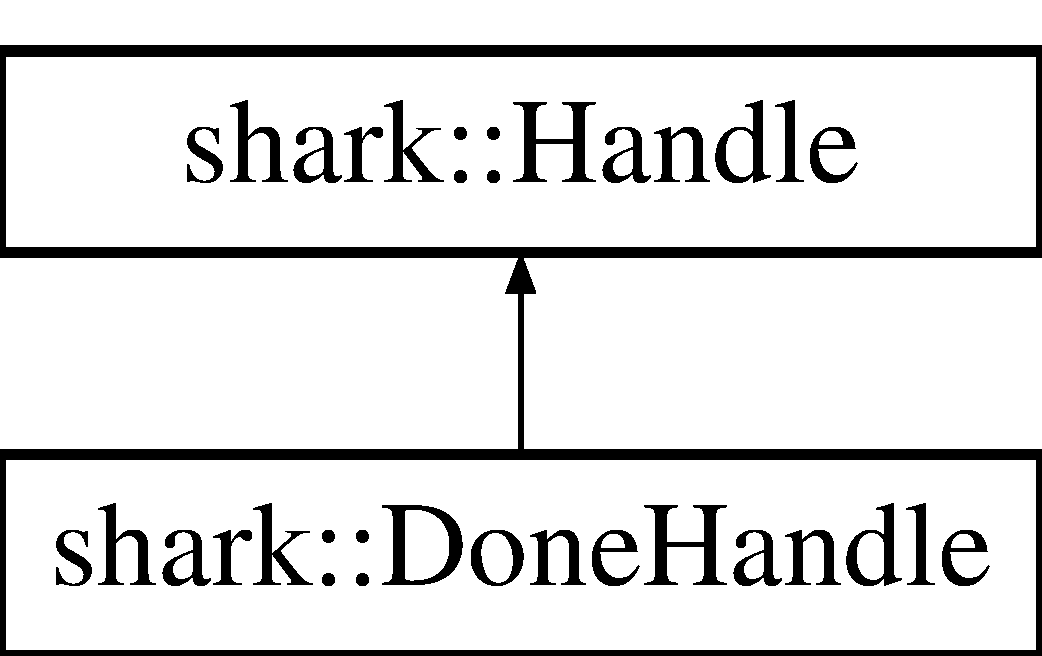
\includegraphics[height=2.000000cm]{classshark_1_1_handle}
\end{center}
\end{figure}
\subsection*{Public Member Functions}
\begin{DoxyCompactItemize}
\item 
\hyperlink{classshark_1_1_handle_a4e3b97f227b72125e595164e0a6629a7}{Handle} ()
\item 
virtual \hyperlink{classshark_1_1_handle_ad63422289041b1a0fbebae079786ae22}{$\sim$\+Handle} ()
\item 
virtual bool \hyperlink{classshark_1_1_handle_a79ac46bc643e22c2a1fb28d45634fa68}{test} ()=0
\item 
virtual void \hyperlink{classshark_1_1_handle_a36117a898368730a1619a1a771cca424}{wait} ()=0
\end{DoxyCompactItemize}
\subsection*{Static Public Member Functions}
\begin{DoxyCompactItemize}
\item 
static void \hyperlink{classshark_1_1_handle_a2c999eeeb8dd6283b9b792515a10e6aa}{make\+\_\+progress} ()
\end{DoxyCompactItemize}
\subsection*{Static Public Attributes}
\begin{DoxyCompactItemize}
\item 
static std\+::set$<$ std\+::shared\+\_\+ptr$<$ \hyperlink{classshark_1_1_handle}{Handle} $>$ $>$ \hyperlink{classshark_1_1_handle_a0ade8d8ad19d5620c10381a7e26db838}{ongoing}
\end{DoxyCompactItemize}


\subsection{Detailed Description}


Definition at line 18 of file future.\+hpp.



\subsection{Constructor \& Destructor Documentation}
\hypertarget{classshark_1_1_handle_a4e3b97f227b72125e595164e0a6629a7}{}\label{classshark_1_1_handle_a4e3b97f227b72125e595164e0a6629a7} 
\index{shark\+::\+Handle@{shark\+::\+Handle}!Handle@{Handle}}
\index{Handle@{Handle}!shark\+::\+Handle@{shark\+::\+Handle}}
\subsubsection{\texorpdfstring{Handle()}{Handle()}}
{\footnotesize\ttfamily Handle\+::\+Handle (\begin{DoxyParamCaption}{ }\end{DoxyParamCaption})}



Definition at line 24 of file future.\+cpp.


\begin{DoxyCode}
24                \{
25 \}
\end{DoxyCode}
\hypertarget{classshark_1_1_handle_ad63422289041b1a0fbebae079786ae22}{}\label{classshark_1_1_handle_ad63422289041b1a0fbebae079786ae22} 
\index{shark\+::\+Handle@{shark\+::\+Handle}!````~Handle@{$\sim$\+Handle}}
\index{````~Handle@{$\sim$\+Handle}!shark\+::\+Handle@{shark\+::\+Handle}}
\subsubsection{\texorpdfstring{$\sim$\+Handle()}{~Handle()}}
{\footnotesize\ttfamily Handle\+::$\sim$\+Handle (\begin{DoxyParamCaption}{ }\end{DoxyParamCaption})\hspace{0.3cm}{\ttfamily [virtual]}}



Definition at line 27 of file future.\+cpp.


\begin{DoxyCode}
27                 \{
28 \}
\end{DoxyCode}


\subsection{Member Function Documentation}
\hypertarget{classshark_1_1_handle_a2c999eeeb8dd6283b9b792515a10e6aa}{}\label{classshark_1_1_handle_a2c999eeeb8dd6283b9b792515a10e6aa} 
\index{shark\+::\+Handle@{shark\+::\+Handle}!make\+\_\+progress@{make\+\_\+progress}}
\index{make\+\_\+progress@{make\+\_\+progress}!shark\+::\+Handle@{shark\+::\+Handle}}
\subsubsection{\texorpdfstring{make\+\_\+progress()}{make\_progress()}}
{\footnotesize\ttfamily void Handle\+::make\+\_\+progress (\begin{DoxyParamCaption}{ }\end{DoxyParamCaption})\hspace{0.3cm}{\ttfamily [static]}}



Definition at line 17 of file future.\+cpp.


\begin{DoxyCode}
17                            \{
18     \textcolor{keywordflow}{for} (\textcolor{keyword}{auto} it = \hyperlink{classshark_1_1_handle_a0ade8d8ad19d5620c10381a7e26db838}{ongoing}.begin(); it != \hyperlink{classshark_1_1_handle_a0ade8d8ad19d5620c10381a7e26db838}{ongoing}.end(); ) \{
19         \textcolor{keywordflow}{if} ((*it)->test()) it = \hyperlink{classshark_1_1_handle_a0ade8d8ad19d5620c10381a7e26db838}{ongoing}.erase(it);
20         \textcolor{keywordflow}{else} ++it;
21     \}
22 \}
\end{DoxyCode}
\hypertarget{classshark_1_1_handle_a79ac46bc643e22c2a1fb28d45634fa68}{}\label{classshark_1_1_handle_a79ac46bc643e22c2a1fb28d45634fa68} 
\index{shark\+::\+Handle@{shark\+::\+Handle}!test@{test}}
\index{test@{test}!shark\+::\+Handle@{shark\+::\+Handle}}
\subsubsection{\texorpdfstring{test()}{test()}}
{\footnotesize\ttfamily virtual bool shark\+::\+Handle\+::test (\begin{DoxyParamCaption}{ }\end{DoxyParamCaption})\hspace{0.3cm}{\ttfamily [pure virtual]}}



Implemented in \hyperlink{classshark_1_1_done_handle_aa2207dc4b61f0bffcbfb56aa9f9b0b46}{shark\+::\+Done\+Handle}.

\hypertarget{classshark_1_1_handle_a36117a898368730a1619a1a771cca424}{}\label{classshark_1_1_handle_a36117a898368730a1619a1a771cca424} 
\index{shark\+::\+Handle@{shark\+::\+Handle}!wait@{wait}}
\index{wait@{wait}!shark\+::\+Handle@{shark\+::\+Handle}}
\subsubsection{\texorpdfstring{wait()}{wait()}}
{\footnotesize\ttfamily virtual void shark\+::\+Handle\+::wait (\begin{DoxyParamCaption}{ }\end{DoxyParamCaption})\hspace{0.3cm}{\ttfamily [pure virtual]}}



Implemented in \hyperlink{classshark_1_1_done_handle_a99b4b58b01738073650b9c452e35b7e8}{shark\+::\+Done\+Handle}.



\subsection{Member Data Documentation}
\hypertarget{classshark_1_1_handle_a0ade8d8ad19d5620c10381a7e26db838}{}\label{classshark_1_1_handle_a0ade8d8ad19d5620c10381a7e26db838} 
\index{shark\+::\+Handle@{shark\+::\+Handle}!ongoing@{ongoing}}
\index{ongoing@{ongoing}!shark\+::\+Handle@{shark\+::\+Handle}}
\subsubsection{\texorpdfstring{ongoing}{ongoing}}
{\footnotesize\ttfamily std\+::set$<$ std\+::shared\+\_\+ptr$<$ \hyperlink{classshark_1_1_handle}{Handle} $>$ $>$ Handle\+::ongoing\hspace{0.3cm}{\ttfamily [static]}}



Definition at line 20 of file future.\+hpp.



The documentation for this class was generated from the following files\+:\begin{DoxyCompactItemize}
\item 
include/shark/\hyperlink{future_8hpp}{future.\+hpp}\item 
src/\hyperlink{future_8cpp}{future.\+cpp}\end{DoxyCompactItemize}

\hypertarget{classshark_1_1ndim_1_1is__source}{}\section{shark\+:\+:ndim\+:\+:is\+\_\+source$<$ S $>$ Class Template Reference}
\label{classshark_1_1ndim_1_1is__source}\index{shark\+::ndim\+::is\+\_\+source$<$ S $>$@{shark\+::ndim\+::is\+\_\+source$<$ S $>$}}


{\ttfamily \#include $<$expr.\+hpp$>$}

\subsection*{Public Attributes}
\begin{DoxyCompactItemize}
\item 
decltype(\hyperlink{classshark_1_1ndim_1_1is__source_a3aae092d2fe4e1593d3997fa4c33c27b}{test}$<$ S $>$(0)) typedef \hyperlink{classshark_1_1ndim_1_1is__source_a8f572031c798bd5661798790582835b2}{result\+\_\+type}
\end{DoxyCompactItemize}
\subsection*{Static Public Attributes}
\begin{DoxyCompactItemize}
\item 
static const bool \hyperlink{classshark_1_1ndim_1_1is__source_a454596d26b3920a0a3e99ebc76362e7c}{value} = result\+\_\+type\+::value
\end{DoxyCompactItemize}
\subsection*{Static Private Member Functions}
\begin{DoxyCompactItemize}
\item 
{\footnotesize template$<$typename T $>$ }\\static std\+::true\+\_\+type \hyperlink{classshark_1_1ndim_1_1is__source_a3aae092d2fe4e1593d3997fa4c33c27b}{test} (decltype(T\+::number\+\_\+of\+\_\+dimensions) $\ast$)
\item 
{\footnotesize template$<$typename $>$ }\\static std\+::false\+\_\+type \hyperlink{classshark_1_1ndim_1_1is__source_a43983e36462efe2c8ff1a5be7e1b30af}{test} (...)
\end{DoxyCompactItemize}


\subsection{Detailed Description}
\subsubsection*{template$<$typename S$>$\newline
class shark\+::ndim\+::is\+\_\+source$<$ S $>$}



Definition at line 28 of file expr.\+hpp.



\subsection{Member Function Documentation}
\hypertarget{classshark_1_1ndim_1_1is__source_a3aae092d2fe4e1593d3997fa4c33c27b}{}\label{classshark_1_1ndim_1_1is__source_a3aae092d2fe4e1593d3997fa4c33c27b} 
\index{shark\+::ndim\+::is\+\_\+source@{shark\+::ndim\+::is\+\_\+source}!test@{test}}
\index{test@{test}!shark\+::ndim\+::is\+\_\+source@{shark\+::ndim\+::is\+\_\+source}}
\subsubsection{\texorpdfstring{test()}{test()}\hspace{0.1cm}{\footnotesize\ttfamily [1/2]}}
{\footnotesize\ttfamily template$<$typename S $>$ \\
template$<$typename T $>$ \\
static std\+::true\+\_\+type \hyperlink{classshark_1_1ndim_1_1is__source}{shark\+::ndim\+::is\+\_\+source}$<$ S $>$\+::test (\begin{DoxyParamCaption}\item[{decltype(T\+::number\+\_\+of\+\_\+dimensions) $\ast$}]{ }\end{DoxyParamCaption})\hspace{0.3cm}{\ttfamily [static]}, {\ttfamily [private]}}

\hypertarget{classshark_1_1ndim_1_1is__source_a43983e36462efe2c8ff1a5be7e1b30af}{}\label{classshark_1_1ndim_1_1is__source_a43983e36462efe2c8ff1a5be7e1b30af} 
\index{shark\+::ndim\+::is\+\_\+source@{shark\+::ndim\+::is\+\_\+source}!test@{test}}
\index{test@{test}!shark\+::ndim\+::is\+\_\+source@{shark\+::ndim\+::is\+\_\+source}}
\subsubsection{\texorpdfstring{test()}{test()}\hspace{0.1cm}{\footnotesize\ttfamily [2/2]}}
{\footnotesize\ttfamily template$<$typename S $>$ \\
template$<$typename $>$ \\
static std\+::false\+\_\+type \hyperlink{classshark_1_1ndim_1_1is__source}{shark\+::ndim\+::is\+\_\+source}$<$ S $>$\+::test (\begin{DoxyParamCaption}\item[{}]{... }\end{DoxyParamCaption})\hspace{0.3cm}{\ttfamily [static]}, {\ttfamily [private]}}



\subsection{Member Data Documentation}
\hypertarget{classshark_1_1ndim_1_1is__source_a8f572031c798bd5661798790582835b2}{}\label{classshark_1_1ndim_1_1is__source_a8f572031c798bd5661798790582835b2} 
\index{shark\+::ndim\+::is\+\_\+source@{shark\+::ndim\+::is\+\_\+source}!result\+\_\+type@{result\+\_\+type}}
\index{result\+\_\+type@{result\+\_\+type}!shark\+::ndim\+::is\+\_\+source@{shark\+::ndim\+::is\+\_\+source}}
\subsubsection{\texorpdfstring{result\+\_\+type}{result\_type}}
{\footnotesize\ttfamily template$<$typename S $>$ \\
decltype(\hyperlink{classshark_1_1ndim_1_1is__source_a3aae092d2fe4e1593d3997fa4c33c27b}{test}$<$S$>$(0)) typedef \hyperlink{classshark_1_1ndim_1_1is__source}{shark\+::ndim\+::is\+\_\+source}$<$ S $>$\+::result\+\_\+type}



Definition at line 35 of file expr.\+hpp.

\hypertarget{classshark_1_1ndim_1_1is__source_a454596d26b3920a0a3e99ebc76362e7c}{}\label{classshark_1_1ndim_1_1is__source_a454596d26b3920a0a3e99ebc76362e7c} 
\index{shark\+::ndim\+::is\+\_\+source@{shark\+::ndim\+::is\+\_\+source}!value@{value}}
\index{value@{value}!shark\+::ndim\+::is\+\_\+source@{shark\+::ndim\+::is\+\_\+source}}
\subsubsection{\texorpdfstring{value}{value}}
{\footnotesize\ttfamily template$<$typename S $>$ \\
const bool \hyperlink{classshark_1_1ndim_1_1is__source}{shark\+::ndim\+::is\+\_\+source}$<$ S $>$\+::value = result\+\_\+type\+::value\hspace{0.3cm}{\ttfamily [static]}}



Definition at line 36 of file expr.\+hpp.



The documentation for this class was generated from the following file\+:\begin{DoxyCompactItemize}
\item 
include/shark/\hyperlink{expr_8hpp}{expr.\+hpp}\end{DoxyCompactItemize}

\hypertarget{classshark_1_1ndim_1_1_max_element}{}\section{shark\+:\+:ndim\+:\+:Max\+Element$<$ S $>$ Class Template Reference}
\label{classshark_1_1ndim_1_1_max_element}\index{shark\+::ndim\+::\+Max\+Element$<$ S $>$@{shark\+::ndim\+::\+Max\+Element$<$ S $>$}}


{\ttfamily \#include $<$expr.\+hpp$>$}

\subsection*{Public Member Functions}
\begin{DoxyCompactItemize}
\item 
auto \hyperlink{classshark_1_1ndim_1_1_max_element_a7130c9b87070f3ff75bc5325f673898a}{operator()} (const typename S\+::accessor \&a, \hyperlink{structshark_1_1ndim_1_1coords}{coords}$<$ S\+::number\+\_\+of\+\_\+dimensions $>$ ii) const -\/$>$ decltype(a(ii).max())
\end{DoxyCompactItemize}


\subsection{Detailed Description}
\subsubsection*{template$<$typename S$>$\newline
class shark\+::ndim\+::\+Max\+Element$<$ S $>$}



Definition at line 632 of file expr.\+hpp.



\subsection{Member Function Documentation}
\hypertarget{classshark_1_1ndim_1_1_max_element_a7130c9b87070f3ff75bc5325f673898a}{}\label{classshark_1_1ndim_1_1_max_element_a7130c9b87070f3ff75bc5325f673898a} 
\index{shark\+::ndim\+::\+Max\+Element@{shark\+::ndim\+::\+Max\+Element}!operator()@{operator()}}
\index{operator()@{operator()}!shark\+::ndim\+::\+Max\+Element@{shark\+::ndim\+::\+Max\+Element}}
\subsubsection{\texorpdfstring{operator()()}{operator()()}}
{\footnotesize\ttfamily template$<$typename S $>$ \\
auto \hyperlink{classshark_1_1ndim_1_1_max_element}{shark\+::ndim\+::\+Max\+Element}$<$ S $>$\+::operator() (\begin{DoxyParamCaption}\item[{const typename S\+::accessor \&}]{a,  }\item[{\hyperlink{structshark_1_1ndim_1_1coords}{coords}$<$ S\+::number\+\_\+of\+\_\+dimensions $>$}]{ii }\end{DoxyParamCaption}) const -\/$>$ decltype(a(ii).max()) \hspace{0.3cm}{\ttfamily [inline]}}



Definition at line 634 of file expr.\+hpp.


\begin{DoxyCode}
634                                                                                                            
                     \{
635                 \textcolor{keywordflow}{return} a(ii).max();
636             \}
\end{DoxyCode}


The documentation for this class was generated from the following file\+:\begin{DoxyCompactItemize}
\item 
include/shark/\hyperlink{expr_8hpp}{expr.\+hpp}\end{DoxyCompactItemize}

\hypertarget{classshark_1_1ndim_1_1_min_element}{}\section{shark\+:\+:ndim\+:\+:Min\+Element$<$ S $>$ Class Template Reference}
\label{classshark_1_1ndim_1_1_min_element}\index{shark\+::ndim\+::\+Min\+Element$<$ S $>$@{shark\+::ndim\+::\+Min\+Element$<$ S $>$}}


{\ttfamily \#include $<$expr.\+hpp$>$}

\subsection*{Public Member Functions}
\begin{DoxyCompactItemize}
\item 
auto \hyperlink{classshark_1_1ndim_1_1_min_element_a86825d644a64c6ad07cd34e18da611bd}{operator()} (const typename S\+::accessor \&a, \hyperlink{structshark_1_1ndim_1_1coords}{coords}$<$ S\+::number\+\_\+of\+\_\+dimensions $>$ ii) const -\/$>$ decltype(a(ii).min())
\end{DoxyCompactItemize}


\subsection{Detailed Description}
\subsubsection*{template$<$typename S$>$\newline
class shark\+::ndim\+::\+Min\+Element$<$ S $>$}

Minimal/maximal element 

Definition at line 624 of file expr.\+hpp.



\subsection{Member Function Documentation}
\hypertarget{classshark_1_1ndim_1_1_min_element_a86825d644a64c6ad07cd34e18da611bd}{}\label{classshark_1_1ndim_1_1_min_element_a86825d644a64c6ad07cd34e18da611bd} 
\index{shark\+::ndim\+::\+Min\+Element@{shark\+::ndim\+::\+Min\+Element}!operator()@{operator()}}
\index{operator()@{operator()}!shark\+::ndim\+::\+Min\+Element@{shark\+::ndim\+::\+Min\+Element}}
\subsubsection{\texorpdfstring{operator()()}{operator()()}}
{\footnotesize\ttfamily template$<$typename S $>$ \\
auto \hyperlink{classshark_1_1ndim_1_1_min_element}{shark\+::ndim\+::\+Min\+Element}$<$ S $>$\+::operator() (\begin{DoxyParamCaption}\item[{const typename S\+::accessor \&}]{a,  }\item[{\hyperlink{structshark_1_1ndim_1_1coords}{coords}$<$ S\+::number\+\_\+of\+\_\+dimensions $>$}]{ii }\end{DoxyParamCaption}) const -\/$>$ decltype(a(ii).min()) \hspace{0.3cm}{\ttfamily [inline]}}



Definition at line 626 of file expr.\+hpp.


\begin{DoxyCode}
626                                                                                                            
                     \{
627                 \textcolor{keywordflow}{return} a(ii).min();
628             \}
\end{DoxyCode}


The documentation for this class was generated from the following file\+:\begin{DoxyCompactItemize}
\item 
include/shark/\hyperlink{expr_8hpp}{expr.\+hpp}\end{DoxyCompactItemize}

\hypertarget{classshark_1_1ndim_1_1_mul}{}\section{shark\+:\+:ndim\+:\+:Mul$<$ S1, S2 $>$ Class Template Reference}
\label{classshark_1_1ndim_1_1_mul}\index{shark\+::ndim\+::\+Mul$<$ S1, S2 $>$@{shark\+::ndim\+::\+Mul$<$ S1, S2 $>$}}


{\ttfamily \#include $<$expr.\+hpp$>$}

\subsection*{Public Member Functions}
\begin{DoxyCompactItemize}
\item 
auto \hyperlink{classshark_1_1ndim_1_1_mul_aa9fc86ff1e8093c5f9c219f5f01d0428}{operator()} (const typename S1\+::accessor \&a1, const typename S2\+::accessor \&a2, \hyperlink{structshark_1_1ndim_1_1coords}{coords}$<$ S1\+::number\+\_\+of\+\_\+dimensions $>$ ii) const -\/$>$ decltype(a1(ii) $\ast$a2(ii))
\end{DoxyCompactItemize}


\subsection{Detailed Description}
\subsubsection*{template$<$typename S1, typename S2$>$\newline
class shark\+::ndim\+::\+Mul$<$ S1, S2 $>$}



Definition at line 805 of file expr.\+hpp.



\subsection{Member Function Documentation}
\hypertarget{classshark_1_1ndim_1_1_mul_aa9fc86ff1e8093c5f9c219f5f01d0428}{}\label{classshark_1_1ndim_1_1_mul_aa9fc86ff1e8093c5f9c219f5f01d0428} 
\index{shark\+::ndim\+::\+Mul@{shark\+::ndim\+::\+Mul}!operator()@{operator()}}
\index{operator()@{operator()}!shark\+::ndim\+::\+Mul@{shark\+::ndim\+::\+Mul}}
\subsubsection{\texorpdfstring{operator()()}{operator()()}}
{\footnotesize\ttfamily template$<$typename S1 , typename S2 $>$ \\
auto \hyperlink{classshark_1_1ndim_1_1_mul}{shark\+::ndim\+::\+Mul}$<$ S1, S2 $>$\+::operator() (\begin{DoxyParamCaption}\item[{const typename S1\+::accessor \&}]{a1,  }\item[{const typename S2\+::accessor \&}]{a2,  }\item[{\hyperlink{structshark_1_1ndim_1_1coords}{coords}$<$ S1\+::number\+\_\+of\+\_\+dimensions $>$}]{ii }\end{DoxyParamCaption}) const -\/$>$ decltype(a1(ii) $\ast$ a2(ii)) \hspace{0.3cm}{\ttfamily [inline]}}



Definition at line 807 of file expr.\+hpp.


\begin{DoxyCode}
807                                                                                                            
                                                           \{
808                 \textcolor{keywordflow}{return} a1(ii) * a2(ii);
809             \}
\end{DoxyCode}


The documentation for this class was generated from the following file\+:\begin{DoxyCompactItemize}
\item 
include/shark/\hyperlink{expr_8hpp}{expr.\+hpp}\end{DoxyCompactItemize}

\hypertarget{classshark_1_1ndim_1_1_mul_c}{}\section{shark\+:\+:ndim\+:\+:MulC$<$ S, T $>$ Class Template Reference}
\label{classshark_1_1ndim_1_1_mul_c}\index{shark\+::ndim\+::\+Mul\+C$<$ S, T $>$@{shark\+::ndim\+::\+Mul\+C$<$ S, T $>$}}


{\ttfamily \#include $<$expr.\+hpp$>$}

\subsection*{Public Member Functions}
\begin{DoxyCompactItemize}
\item 
\hyperlink{classshark_1_1ndim_1_1_mul_c_aea6eccffd6c63cc792714e48c9dc1c9e}{MulC} (const T \&\hyperlink{classshark_1_1ndim_1_1_mul_c_adf2e920c0c3a31d93f551ba6d75170cd}{val})
\item 
\hyperlink{classshark_1_1ndim_1_1_mul_c_a045d8909667e5ccf881459f35119b74e}{$\sim$\+MulC} ()
\item 
auto \hyperlink{classshark_1_1ndim_1_1_mul_c_a81f80d754e0c9852bcf6ce4f58a55c64}{operator()} (const typename S\+::accessor \&a, \hyperlink{structshark_1_1ndim_1_1coords}{coords}$<$ S\+::number\+\_\+of\+\_\+dimensions $>$ ii) const -\/$>$ decltype(a(ii) $\ast$\hyperlink{classshark_1_1ndim_1_1_mul_c_adf2e920c0c3a31d93f551ba6d75170cd}{val})
\end{DoxyCompactItemize}
\subsection*{Private Attributes}
\begin{DoxyCompactItemize}
\item 
const T \hyperlink{classshark_1_1ndim_1_1_mul_c_adf2e920c0c3a31d93f551ba6d75170cd}{val}
\end{DoxyCompactItemize}


\subsection{Detailed Description}
\subsubsection*{template$<$typename S, typename T$>$\newline
class shark\+::ndim\+::\+Mul\+C$<$ S, T $>$}

Multiplication 

Definition at line 783 of file expr.\+hpp.



\subsection{Constructor \& Destructor Documentation}
\hypertarget{classshark_1_1ndim_1_1_mul_c_aea6eccffd6c63cc792714e48c9dc1c9e}{}\label{classshark_1_1ndim_1_1_mul_c_aea6eccffd6c63cc792714e48c9dc1c9e} 
\index{shark\+::ndim\+::\+MulC@{shark\+::ndim\+::\+MulC}!MulC@{MulC}}
\index{MulC@{MulC}!shark\+::ndim\+::\+MulC@{shark\+::ndim\+::\+MulC}}
\subsubsection{\texorpdfstring{Mul\+C()}{MulC()}}
{\footnotesize\ttfamily template$<$typename S , typename T $>$ \\
\hyperlink{classshark_1_1ndim_1_1_mul_c}{shark\+::ndim\+::\+MulC}$<$ S, T $>$\+::\hyperlink{classshark_1_1ndim_1_1_mul_c}{MulC} (\begin{DoxyParamCaption}\item[{const T \&}]{val }\end{DoxyParamCaption})\hspace{0.3cm}{\ttfamily [inline]}}



Definition at line 787 of file expr.\+hpp.


\begin{DoxyCode}
787 : \hyperlink{classshark_1_1ndim_1_1_mul_c_adf2e920c0c3a31d93f551ba6d75170cd}{val}(\hyperlink{classshark_1_1ndim_1_1_mul_c_adf2e920c0c3a31d93f551ba6d75170cd}{val}) \{ \}
\end{DoxyCode}
\hypertarget{classshark_1_1ndim_1_1_mul_c_a045d8909667e5ccf881459f35119b74e}{}\label{classshark_1_1ndim_1_1_mul_c_a045d8909667e5ccf881459f35119b74e} 
\index{shark\+::ndim\+::\+MulC@{shark\+::ndim\+::\+MulC}!````~MulC@{$\sim$\+MulC}}
\index{````~MulC@{$\sim$\+MulC}!shark\+::ndim\+::\+MulC@{shark\+::ndim\+::\+MulC}}
\subsubsection{\texorpdfstring{$\sim$\+Mul\+C()}{~MulC()}}
{\footnotesize\ttfamily template$<$typename S , typename T $>$ \\
\hyperlink{classshark_1_1ndim_1_1_mul_c}{shark\+::ndim\+::\+MulC}$<$ S, T $>$\+::$\sim$\hyperlink{classshark_1_1ndim_1_1_mul_c}{MulC} (\begin{DoxyParamCaption}{ }\end{DoxyParamCaption})\hspace{0.3cm}{\ttfamily [inline]}}



Definition at line 788 of file expr.\+hpp.


\begin{DoxyCode}
788 \{ \}
\end{DoxyCode}


\subsection{Member Function Documentation}
\hypertarget{classshark_1_1ndim_1_1_mul_c_a81f80d754e0c9852bcf6ce4f58a55c64}{}\label{classshark_1_1ndim_1_1_mul_c_a81f80d754e0c9852bcf6ce4f58a55c64} 
\index{shark\+::ndim\+::\+MulC@{shark\+::ndim\+::\+MulC}!operator()@{operator()}}
\index{operator()@{operator()}!shark\+::ndim\+::\+MulC@{shark\+::ndim\+::\+MulC}}
\subsubsection{\texorpdfstring{operator()()}{operator()()}}
{\footnotesize\ttfamily template$<$typename S , typename T $>$ \\
auto \hyperlink{classshark_1_1ndim_1_1_mul_c}{shark\+::ndim\+::\+MulC}$<$ S, T $>$\+::operator() (\begin{DoxyParamCaption}\item[{const typename S\+::accessor \&}]{a,  }\item[{\hyperlink{structshark_1_1ndim_1_1coords}{coords}$<$ S\+::number\+\_\+of\+\_\+dimensions $>$}]{ii }\end{DoxyParamCaption}) const -\/$>$ decltype(a(ii)$\ast$\hyperlink{classshark_1_1ndim_1_1_mul_c_adf2e920c0c3a31d93f551ba6d75170cd}{val}) \hspace{0.3cm}{\ttfamily [inline]}}



Definition at line 789 of file expr.\+hpp.


\begin{DoxyCode}
789                                                                                                            
                   \{
790                 \textcolor{keywordflow}{return} a(ii) * \hyperlink{classshark_1_1ndim_1_1_mul_c_adf2e920c0c3a31d93f551ba6d75170cd}{val};
791             \}
\end{DoxyCode}


\subsection{Member Data Documentation}
\hypertarget{classshark_1_1ndim_1_1_mul_c_adf2e920c0c3a31d93f551ba6d75170cd}{}\label{classshark_1_1ndim_1_1_mul_c_adf2e920c0c3a31d93f551ba6d75170cd} 
\index{shark\+::ndim\+::\+MulC@{shark\+::ndim\+::\+MulC}!val@{val}}
\index{val@{val}!shark\+::ndim\+::\+MulC@{shark\+::ndim\+::\+MulC}}
\subsubsection{\texorpdfstring{val}{val}}
{\footnotesize\ttfamily template$<$typename S , typename T $>$ \\
const T \hyperlink{classshark_1_1ndim_1_1_mul_c}{shark\+::ndim\+::\+MulC}$<$ S, T $>$\+::val\hspace{0.3cm}{\ttfamily [private]}}



Definition at line 785 of file expr.\+hpp.



The documentation for this class was generated from the following file\+:\begin{DoxyCompactItemize}
\item 
include/shark/\hyperlink{expr_8hpp}{expr.\+hpp}\end{DoxyCompactItemize}

\hypertarget{classshark_1_1ndim_1_1_neg}{}\section{shark\+:\+:ndim\+:\+:Neg$<$ S $>$ Class Template Reference}
\label{classshark_1_1ndim_1_1_neg}\index{shark\+::ndim\+::\+Neg$<$ S $>$@{shark\+::ndim\+::\+Neg$<$ S $>$}}


{\ttfamily \#include $<$expr.\+hpp$>$}

\subsection*{Public Member Functions}
\begin{DoxyCompactItemize}
\item 
auto \hyperlink{classshark_1_1ndim_1_1_neg_a36cc3e8ae8bac2421a59271e47f56000}{operator()} (const typename S\+::accessor \&a, \hyperlink{structshark_1_1ndim_1_1coords}{coords}$<$ S\+::number\+\_\+of\+\_\+dimensions $>$ ii) const -\/$>$ decltype(-\/a(ii))
\end{DoxyCompactItemize}


\subsection{Detailed Description}
\subsubsection*{template$<$typename S$>$\newline
class shark\+::ndim\+::\+Neg$<$ S $>$}

Negation 

Definition at line 565 of file expr.\+hpp.



\subsection{Member Function Documentation}
\hypertarget{classshark_1_1ndim_1_1_neg_a36cc3e8ae8bac2421a59271e47f56000}{}\label{classshark_1_1ndim_1_1_neg_a36cc3e8ae8bac2421a59271e47f56000} 
\index{shark\+::ndim\+::\+Neg@{shark\+::ndim\+::\+Neg}!operator()@{operator()}}
\index{operator()@{operator()}!shark\+::ndim\+::\+Neg@{shark\+::ndim\+::\+Neg}}
\subsubsection{\texorpdfstring{operator()()}{operator()()}}
{\footnotesize\ttfamily template$<$typename S $>$ \\
auto \hyperlink{classshark_1_1ndim_1_1_neg}{shark\+::ndim\+::\+Neg}$<$ S $>$\+::operator() (\begin{DoxyParamCaption}\item[{const typename S\+::accessor \&}]{a,  }\item[{\hyperlink{structshark_1_1ndim_1_1coords}{coords}$<$ S\+::number\+\_\+of\+\_\+dimensions $>$}]{ii }\end{DoxyParamCaption}) const -\/$>$ decltype(-\/a(ii)) \hspace{0.3cm}{\ttfamily [inline]}}



Definition at line 567 of file expr.\+hpp.


\begin{DoxyCode}
567                                                                                                            
                \{
568                 \textcolor{keywordflow}{return} -a(ii);
569             \}
\end{DoxyCode}


The documentation for this class was generated from the following file\+:\begin{DoxyCompactItemize}
\item 
include/shark/\hyperlink{expr_8hpp}{expr.\+hpp}\end{DoxyCompactItemize}

\hypertarget{classshark_1_1ndim_1_1_nullary_acc}{}\section{shark\+:\+:ndim\+:\+:Nullary\+Acc$<$ ndim, Func $>$ Class Template Reference}
\label{classshark_1_1ndim_1_1_nullary_acc}\index{shark\+::ndim\+::\+Nullary\+Acc$<$ ndim, Func $>$@{shark\+::ndim\+::\+Nullary\+Acc$<$ ndim, Func $>$}}


{\ttfamily \#include $<$expr.\+hpp$>$}

\subsection*{Public Member Functions}
\begin{DoxyCompactItemize}
\item 
\hyperlink{classshark_1_1ndim_1_1_nullary_acc_a65629401dcf916c324bff4f5012688ff}{Nullary\+Acc} (const \hyperlink{classshark_1_1ndim_1_1_nullary_exp}{Nullary\+Exp}$<$ ndim, Func $>$ \&exp)
\item 
\hyperlink{classshark_1_1ndim_1_1_nullary_acc_a34d1a64e5e395fb4ca2fa636ee164c1c}{$\sim$\+Nullary\+Acc} ()
\item 
decltype(std\+::declval$<$ Func $>$()(std\+::declval$<$ \hyperlink{structshark_1_1ndim_1_1coords}{coords}$<$ ndim $>$$>$())) \hyperlink{common_8hpp_a2eb6f9e0395b47b8d5e3eeae4fe0c116}{I\+N\+L\+I\+NE} \hyperlink{classshark_1_1ndim_1_1_nullary_acc_a54d80a3d684587e7ca45d780e4832faf}{operator()} (\hyperlink{structshark_1_1ndim_1_1coords}{coords}$<$ ndim $>$ ii) const
\end{DoxyCompactItemize}
\subsection*{Private Attributes}
\begin{DoxyCompactItemize}
\item 
const Func \& \hyperlink{classshark_1_1ndim_1_1_nullary_acc_a2818f289b8c710f249e38a20412cf54d}{f}
\end{DoxyCompactItemize}


\subsection{Detailed Description}
\subsubsection*{template$<$int ndim, typename Func$>$\newline
class shark\+::ndim\+::\+Nullary\+Acc$<$ ndim, Func $>$}

Nullary expressions 

Definition at line 52 of file expr.\+hpp.



\subsection{Constructor \& Destructor Documentation}
\hypertarget{classshark_1_1ndim_1_1_nullary_acc_a65629401dcf916c324bff4f5012688ff}{}\label{classshark_1_1ndim_1_1_nullary_acc_a65629401dcf916c324bff4f5012688ff} 
\index{shark\+::ndim\+::\+Nullary\+Acc@{shark\+::ndim\+::\+Nullary\+Acc}!Nullary\+Acc@{Nullary\+Acc}}
\index{Nullary\+Acc@{Nullary\+Acc}!shark\+::ndim\+::\+Nullary\+Acc@{shark\+::ndim\+::\+Nullary\+Acc}}
\subsubsection{\texorpdfstring{Nullary\+Acc()}{NullaryAcc()}}
{\footnotesize\ttfamily template$<$int ndim, typename Func $>$ \\
\hyperlink{classshark_1_1ndim_1_1_nullary_acc}{shark\+::ndim\+::\+Nullary\+Acc}$<$ ndim, Func $>$\+::\hyperlink{classshark_1_1ndim_1_1_nullary_acc}{Nullary\+Acc} (\begin{DoxyParamCaption}\item[{const \hyperlink{classshark_1_1ndim_1_1_nullary_exp}{Nullary\+Exp}$<$ ndim, Func $>$ \&}]{exp }\end{DoxyParamCaption})}



Definition at line 104 of file expr.\+hpp.


\begin{DoxyCode}
104 : \hyperlink{classshark_1_1ndim_1_1_nullary_acc_a2818f289b8c710f249e38a20412cf54d}{f}(exp.f) \{ \}
\end{DoxyCode}
\hypertarget{classshark_1_1ndim_1_1_nullary_acc_a34d1a64e5e395fb4ca2fa636ee164c1c}{}\label{classshark_1_1ndim_1_1_nullary_acc_a34d1a64e5e395fb4ca2fa636ee164c1c} 
\index{shark\+::ndim\+::\+Nullary\+Acc@{shark\+::ndim\+::\+Nullary\+Acc}!````~Nullary\+Acc@{$\sim$\+Nullary\+Acc}}
\index{````~Nullary\+Acc@{$\sim$\+Nullary\+Acc}!shark\+::ndim\+::\+Nullary\+Acc@{shark\+::ndim\+::\+Nullary\+Acc}}
\subsubsection{\texorpdfstring{$\sim$\+Nullary\+Acc()}{~NullaryAcc()}}
{\footnotesize\ttfamily template$<$int ndim, typename Func $>$ \\
\hyperlink{classshark_1_1ndim_1_1_nullary_acc}{shark\+::ndim\+::\+Nullary\+Acc}$<$ ndim, Func $>$\+::$\sim$\hyperlink{classshark_1_1ndim_1_1_nullary_acc}{Nullary\+Acc} (\begin{DoxyParamCaption}{ }\end{DoxyParamCaption})}



Definition at line 107 of file expr.\+hpp.


\begin{DoxyCode}
107 \{ \}
\end{DoxyCode}


\subsection{Member Function Documentation}
\hypertarget{classshark_1_1ndim_1_1_nullary_acc_a54d80a3d684587e7ca45d780e4832faf}{}\label{classshark_1_1ndim_1_1_nullary_acc_a54d80a3d684587e7ca45d780e4832faf} 
\index{shark\+::ndim\+::\+Nullary\+Acc@{shark\+::ndim\+::\+Nullary\+Acc}!operator()@{operator()}}
\index{operator()@{operator()}!shark\+::ndim\+::\+Nullary\+Acc@{shark\+::ndim\+::\+Nullary\+Acc}}
\subsubsection{\texorpdfstring{operator()()}{operator()()}}
{\footnotesize\ttfamily template$<$int ndim, typename Func $>$ \\
decltype(std\+::declval$<$Func$>$()(std\+::declval$<$\hyperlink{structshark_1_1ndim_1_1coords}{coords}$<$ndim$>$$>$())) \hyperlink{common_8hpp_a2eb6f9e0395b47b8d5e3eeae4fe0c116}{I\+N\+L\+I\+NE} \hyperlink{classshark_1_1ndim_1_1_nullary_acc}{shark\+::ndim\+::\+Nullary\+Acc}$<$ ndim, Func $>$\+::operator() (\begin{DoxyParamCaption}\item[{\hyperlink{structshark_1_1ndim_1_1coords}{coords}$<$ ndim $>$}]{ii }\end{DoxyParamCaption}) const}



\subsection{Member Data Documentation}
\hypertarget{classshark_1_1ndim_1_1_nullary_acc_a2818f289b8c710f249e38a20412cf54d}{}\label{classshark_1_1ndim_1_1_nullary_acc_a2818f289b8c710f249e38a20412cf54d} 
\index{shark\+::ndim\+::\+Nullary\+Acc@{shark\+::ndim\+::\+Nullary\+Acc}!f@{f}}
\index{f@{f}!shark\+::ndim\+::\+Nullary\+Acc@{shark\+::ndim\+::\+Nullary\+Acc}}
\subsubsection{\texorpdfstring{f}{f}}
{\footnotesize\ttfamily template$<$int ndim, typename Func $>$ \\
const Func\& \hyperlink{classshark_1_1ndim_1_1_nullary_acc}{shark\+::ndim\+::\+Nullary\+Acc}$<$ ndim, Func $>$\+::f\hspace{0.3cm}{\ttfamily [private]}}



Definition at line 92 of file expr.\+hpp.



The documentation for this class was generated from the following file\+:\begin{DoxyCompactItemize}
\item 
include/shark/\hyperlink{expr_8hpp}{expr.\+hpp}\end{DoxyCompactItemize}

\hypertarget{classshark_1_1ndim_1_1_nullary_exp}{}\section{shark\+:\+:ndim\+:\+:Nullary\+Exp$<$ ndim, Func $>$ Class Template Reference}
\label{classshark_1_1ndim_1_1_nullary_exp}\index{shark\+::ndim\+::\+Nullary\+Exp$<$ ndim, Func $>$@{shark\+::ndim\+::\+Nullary\+Exp$<$ ndim, Func $>$}}


{\ttfamily \#include $<$expr.\+hpp$>$}

\subsection*{Public Types}
\begin{DoxyCompactItemize}
\item 
typedef \hyperlink{classshark_1_1ndim_1_1_nullary_exp}{Nullary\+Exp}$<$ ndim, Func $>$ \hyperlink{classshark_1_1ndim_1_1_nullary_exp_aaa0a351df054b29eef3d783eb6914ec8}{storage}
\item 
typedef \hyperlink{classshark_1_1ndim_1_1_nullary_acc}{Nullary\+Acc}$<$ ndim, Func $>$ \hyperlink{classshark_1_1ndim_1_1_nullary_exp_a3934c7a6d447182edb34537703afed68}{accessor}
\end{DoxyCompactItemize}
\subsection*{Public Member Functions}
\begin{DoxyCompactItemize}
\item 
\hyperlink{classshark_1_1ndim_1_1_nullary_exp_a8de00bdc6aab3dd30183ac0b79055bbf}{Nullary\+Exp} (const \hyperlink{classshark_1_1ndim_1_1_domain}{Domain}$<$ ndim $>$ \&\hyperlink{classshark_1_1ndim_1_1_nullary_exp_a4af666c034e0035ca4a9c4f8cf2f2ea2}{dom}, const Func \&\hyperlink{classshark_1_1ndim_1_1_nullary_exp_a30f367c05cd7978aedec0a99ca82ed0e}{f})
\item 
\hyperlink{classshark_1_1ndim_1_1_nullary_exp_afb64b1b8dff8c3904b25b6d95125fc71}{Nullary\+Exp} (const \hyperlink{classshark_1_1ndim_1_1_domain}{Domain}$<$ ndim $>$ \&\hyperlink{classshark_1_1ndim_1_1_nullary_exp_a4af666c034e0035ca4a9c4f8cf2f2ea2}{dom}, \hyperlink{structshark_1_1ndim_1_1coords__range}{coords\+\_\+range}$<$ ndim $>$ \hyperlink{classshark_1_1ndim_1_1_nullary_exp_a2ab3c895de1618318f8864c90cd7b21e}{r}, const Func \&\hyperlink{classshark_1_1ndim_1_1_nullary_exp_a30f367c05cd7978aedec0a99ca82ed0e}{f})
\item 
\hyperlink{classshark_1_1ndim_1_1_nullary_exp_a8ec438084517a13c115bd6979023abf1}{$\sim$\+Nullary\+Exp} ()
\item 
\hyperlink{common_8hpp_a2eb6f9e0395b47b8d5e3eeae4fe0c116}{I\+N\+L\+I\+NE} const \hyperlink{classshark_1_1ndim_1_1_domain}{Domain}$<$ ndim $>$ \& \hyperlink{classshark_1_1ndim_1_1_nullary_exp_ae6e867ba02940b7f1204e2910c781a9f}{domain} () const
\item 
\hyperlink{common_8hpp_a2eb6f9e0395b47b8d5e3eeae4fe0c116}{I\+N\+L\+I\+NE} \hyperlink{structshark_1_1ndim_1_1coords__range}{coords\+\_\+range}$<$ ndim $>$ \hyperlink{classshark_1_1ndim_1_1_nullary_exp_a82f2b29d4412c95428e1eda9ff454cf6}{region} () const
\end{DoxyCompactItemize}
\subsection*{Static Public Attributes}
\begin{DoxyCompactItemize}
\item 
static const int \hyperlink{classshark_1_1ndim_1_1_nullary_exp_ae586c786daf51061eb41615d208b2c12}{number\+\_\+of\+\_\+dimensions} = ndim
\end{DoxyCompactItemize}
\subsection*{Private Attributes}
\begin{DoxyCompactItemize}
\item 
const \hyperlink{classshark_1_1ndim_1_1_domain}{Domain}$<$ ndim $>$ \& \hyperlink{classshark_1_1ndim_1_1_nullary_exp_a4af666c034e0035ca4a9c4f8cf2f2ea2}{dom}
\item 
const \hyperlink{structshark_1_1ndim_1_1coords__range}{coords\+\_\+range}$<$ ndim $>$ \hyperlink{classshark_1_1ndim_1_1_nullary_exp_a2ab3c895de1618318f8864c90cd7b21e}{r}
\item 
const Func \hyperlink{classshark_1_1ndim_1_1_nullary_exp_a30f367c05cd7978aedec0a99ca82ed0e}{f}
\end{DoxyCompactItemize}
\subsection*{Friends}
\begin{DoxyCompactItemize}
\item 
class \hyperlink{classshark_1_1ndim_1_1_nullary_exp_aae3b9819be1b386ed4bb69e9a1e44726}{Nullary\+Acc$<$ ndim, Func $>$}
\end{DoxyCompactItemize}


\subsection{Detailed Description}
\subsubsection*{template$<$int ndim, typename Func$>$\newline
class shark\+::ndim\+::\+Nullary\+Exp$<$ ndim, Func $>$}



Definition at line 55 of file expr.\+hpp.



\subsection{Member Typedef Documentation}
\hypertarget{classshark_1_1ndim_1_1_nullary_exp_a3934c7a6d447182edb34537703afed68}{}\label{classshark_1_1ndim_1_1_nullary_exp_a3934c7a6d447182edb34537703afed68} 
\index{shark\+::ndim\+::\+Nullary\+Exp@{shark\+::ndim\+::\+Nullary\+Exp}!accessor@{accessor}}
\index{accessor@{accessor}!shark\+::ndim\+::\+Nullary\+Exp@{shark\+::ndim\+::\+Nullary\+Exp}}
\subsubsection{\texorpdfstring{accessor}{accessor}}
{\footnotesize\ttfamily template$<$int ndim, typename Func$>$ \\
typedef \hyperlink{classshark_1_1ndim_1_1_nullary_acc}{Nullary\+Acc}$<$ndim,Func$>$ \hyperlink{classshark_1_1ndim_1_1_nullary_exp}{shark\+::ndim\+::\+Nullary\+Exp}$<$ ndim, Func $>$\+::\hyperlink{classshark_1_1ndim_1_1_nullary_exp_a3934c7a6d447182edb34537703afed68}{accessor}}



Definition at line 63 of file expr.\+hpp.

\hypertarget{classshark_1_1ndim_1_1_nullary_exp_aaa0a351df054b29eef3d783eb6914ec8}{}\label{classshark_1_1ndim_1_1_nullary_exp_aaa0a351df054b29eef3d783eb6914ec8} 
\index{shark\+::ndim\+::\+Nullary\+Exp@{shark\+::ndim\+::\+Nullary\+Exp}!storage@{storage}}
\index{storage@{storage}!shark\+::ndim\+::\+Nullary\+Exp@{shark\+::ndim\+::\+Nullary\+Exp}}
\subsubsection{\texorpdfstring{storage}{storage}}
{\footnotesize\ttfamily template$<$int ndim, typename Func$>$ \\
typedef \hyperlink{classshark_1_1ndim_1_1_nullary_exp}{Nullary\+Exp}$<$ndim,Func$>$ \hyperlink{classshark_1_1ndim_1_1_nullary_exp}{shark\+::ndim\+::\+Nullary\+Exp}$<$ ndim, Func $>$\+::\hyperlink{classshark_1_1ndim_1_1_nullary_exp_aaa0a351df054b29eef3d783eb6914ec8}{storage}}



Definition at line 62 of file expr.\+hpp.



\subsection{Constructor \& Destructor Documentation}
\hypertarget{classshark_1_1ndim_1_1_nullary_exp_a8de00bdc6aab3dd30183ac0b79055bbf}{}\label{classshark_1_1ndim_1_1_nullary_exp_a8de00bdc6aab3dd30183ac0b79055bbf} 
\index{shark\+::ndim\+::\+Nullary\+Exp@{shark\+::ndim\+::\+Nullary\+Exp}!Nullary\+Exp@{Nullary\+Exp}}
\index{Nullary\+Exp@{Nullary\+Exp}!shark\+::ndim\+::\+Nullary\+Exp@{shark\+::ndim\+::\+Nullary\+Exp}}
\subsubsection{\texorpdfstring{Nullary\+Exp()}{NullaryExp()}\hspace{0.1cm}{\footnotesize\ttfamily [1/2]}}
{\footnotesize\ttfamily template$<$int ndim, typename Func $>$ \\
\hyperlink{classshark_1_1ndim_1_1_nullary_exp}{shark\+::ndim\+::\+Nullary\+Exp}$<$ ndim, Func $>$\+::\hyperlink{classshark_1_1ndim_1_1_nullary_exp}{Nullary\+Exp} (\begin{DoxyParamCaption}\item[{const \hyperlink{classshark_1_1ndim_1_1_domain}{Domain}$<$ ndim $>$ \&}]{dom,  }\item[{const Func \&}]{f }\end{DoxyParamCaption})}



Definition at line 72 of file expr.\+hpp.


\begin{DoxyCode}
72 : \hyperlink{classshark_1_1ndim_1_1_nullary_exp_a4af666c034e0035ca4a9c4f8cf2f2ea2}{dom}(\hyperlink{classshark_1_1ndim_1_1_nullary_exp_a4af666c034e0035ca4a9c4f8cf2f2ea2}{dom}), \hyperlink{classshark_1_1ndim_1_1_nullary_exp_a2ab3c895de1618318f8864c90cd7b21e}{r}(\hyperlink{classshark_1_1ndim_1_1_nullary_exp_a4af666c034e0035ca4a9c4f8cf2f2ea2}{dom}.total()), \hyperlink{classshark_1_1ndim_1_1_nullary_exp_a30f367c05cd7978aedec0a99ca82ed0e}{f}(\hyperlink{classshark_1_1ndim_1_1_nullary_exp_a30f367c05cd7978aedec0a99ca82ed0e}{f}) \{ \}
\end{DoxyCode}
\hypertarget{classshark_1_1ndim_1_1_nullary_exp_afb64b1b8dff8c3904b25b6d95125fc71}{}\label{classshark_1_1ndim_1_1_nullary_exp_afb64b1b8dff8c3904b25b6d95125fc71} 
\index{shark\+::ndim\+::\+Nullary\+Exp@{shark\+::ndim\+::\+Nullary\+Exp}!Nullary\+Exp@{Nullary\+Exp}}
\index{Nullary\+Exp@{Nullary\+Exp}!shark\+::ndim\+::\+Nullary\+Exp@{shark\+::ndim\+::\+Nullary\+Exp}}
\subsubsection{\texorpdfstring{Nullary\+Exp()}{NullaryExp()}\hspace{0.1cm}{\footnotesize\ttfamily [2/2]}}
{\footnotesize\ttfamily template$<$int ndim, typename Func $>$ \\
\hyperlink{classshark_1_1ndim_1_1_nullary_exp}{shark\+::ndim\+::\+Nullary\+Exp}$<$ ndim, Func $>$\+::\hyperlink{classshark_1_1ndim_1_1_nullary_exp}{Nullary\+Exp} (\begin{DoxyParamCaption}\item[{const \hyperlink{classshark_1_1ndim_1_1_domain}{Domain}$<$ ndim $>$ \&}]{dom,  }\item[{\hyperlink{structshark_1_1ndim_1_1coords__range}{coords\+\_\+range}$<$ ndim $>$}]{r,  }\item[{const Func \&}]{f }\end{DoxyParamCaption})}



Definition at line 75 of file expr.\+hpp.


\begin{DoxyCode}
75 : \hyperlink{classshark_1_1ndim_1_1_nullary_exp_a4af666c034e0035ca4a9c4f8cf2f2ea2}{dom}(\hyperlink{classshark_1_1ndim_1_1_nullary_exp_a4af666c034e0035ca4a9c4f8cf2f2ea2}{dom}), \hyperlink{classshark_1_1ndim_1_1_nullary_exp_a2ab3c895de1618318f8864c90cd7b21e}{r}(\hyperlink{classshark_1_1ndim_1_1_nullary_exp_a2ab3c895de1618318f8864c90cd7b21e}{r}), \hyperlink{classshark_1_1ndim_1_1_nullary_exp_a30f367c05cd7978aedec0a99ca82ed0e}{f}(\hyperlink{classshark_1_1ndim_1_1_nullary_exp_a30f367c05cd7978aedec0a99ca82ed0e}{f}) \{ \}
\end{DoxyCode}
\hypertarget{classshark_1_1ndim_1_1_nullary_exp_a8ec438084517a13c115bd6979023abf1}{}\label{classshark_1_1ndim_1_1_nullary_exp_a8ec438084517a13c115bd6979023abf1} 
\index{shark\+::ndim\+::\+Nullary\+Exp@{shark\+::ndim\+::\+Nullary\+Exp}!````~Nullary\+Exp@{$\sim$\+Nullary\+Exp}}
\index{````~Nullary\+Exp@{$\sim$\+Nullary\+Exp}!shark\+::ndim\+::\+Nullary\+Exp@{shark\+::ndim\+::\+Nullary\+Exp}}
\subsubsection{\texorpdfstring{$\sim$\+Nullary\+Exp()}{~NullaryExp()}}
{\footnotesize\ttfamily template$<$int ndim, typename Func $>$ \\
\hyperlink{classshark_1_1ndim_1_1_nullary_exp}{shark\+::ndim\+::\+Nullary\+Exp}$<$ ndim, Func $>$\+::$\sim$\hyperlink{classshark_1_1ndim_1_1_nullary_exp}{Nullary\+Exp} (\begin{DoxyParamCaption}{ }\end{DoxyParamCaption})}



Definition at line 78 of file expr.\+hpp.


\begin{DoxyCode}
78 \{ \}
\end{DoxyCode}


\subsection{Member Function Documentation}
\hypertarget{classshark_1_1ndim_1_1_nullary_exp_ae6e867ba02940b7f1204e2910c781a9f}{}\label{classshark_1_1ndim_1_1_nullary_exp_ae6e867ba02940b7f1204e2910c781a9f} 
\index{shark\+::ndim\+::\+Nullary\+Exp@{shark\+::ndim\+::\+Nullary\+Exp}!domain@{domain}}
\index{domain@{domain}!shark\+::ndim\+::\+Nullary\+Exp@{shark\+::ndim\+::\+Nullary\+Exp}}
\subsubsection{\texorpdfstring{domain()}{domain()}}
{\footnotesize\ttfamily template$<$int ndim, typename Func $>$ \\
const \hyperlink{classshark_1_1ndim_1_1_domain}{Domain}$<$ ndim $>$ \& \hyperlink{classshark_1_1ndim_1_1_nullary_exp}{shark\+::ndim\+::\+Nullary\+Exp}$<$ ndim, Func $>$\+::domain (\begin{DoxyParamCaption}{ }\end{DoxyParamCaption}) const\hspace{0.3cm}{\ttfamily [inline]}}



Definition at line 81 of file expr.\+hpp.


\begin{DoxyCode}
81                                                                        \{
82             \textcolor{keywordflow}{return} \hyperlink{classshark_1_1ndim_1_1_nullary_exp_a4af666c034e0035ca4a9c4f8cf2f2ea2}{dom};
83         \}
\end{DoxyCode}
\hypertarget{classshark_1_1ndim_1_1_nullary_exp_a82f2b29d4412c95428e1eda9ff454cf6}{}\label{classshark_1_1ndim_1_1_nullary_exp_a82f2b29d4412c95428e1eda9ff454cf6} 
\index{shark\+::ndim\+::\+Nullary\+Exp@{shark\+::ndim\+::\+Nullary\+Exp}!region@{region}}
\index{region@{region}!shark\+::ndim\+::\+Nullary\+Exp@{shark\+::ndim\+::\+Nullary\+Exp}}
\subsubsection{\texorpdfstring{region()}{region()}}
{\footnotesize\ttfamily template$<$int ndim, typename Func $>$ \\
\hyperlink{structshark_1_1ndim_1_1coords__range}{coords\+\_\+range}$<$ ndim $>$ \hyperlink{classshark_1_1ndim_1_1_nullary_exp}{shark\+::ndim\+::\+Nullary\+Exp}$<$ ndim, Func $>$\+::region (\begin{DoxyParamCaption}{ }\end{DoxyParamCaption}) const\hspace{0.3cm}{\ttfamily [inline]}}



Definition at line 86 of file expr.\+hpp.


\begin{DoxyCode}
86                                                                       \{
87             \textcolor{keywordflow}{return} \hyperlink{classshark_1_1ndim_1_1_nullary_exp_a2ab3c895de1618318f8864c90cd7b21e}{r};
88         \}
\end{DoxyCode}


\subsection{Friends And Related Function Documentation}
\hypertarget{classshark_1_1ndim_1_1_nullary_exp_aae3b9819be1b386ed4bb69e9a1e44726}{}\label{classshark_1_1ndim_1_1_nullary_exp_aae3b9819be1b386ed4bb69e9a1e44726} 
\index{shark\+::ndim\+::\+Nullary\+Exp@{shark\+::ndim\+::\+Nullary\+Exp}!Nullary\+Acc$<$ ndim, Func $>$@{Nullary\+Acc$<$ ndim, Func $>$}}
\index{Nullary\+Acc$<$ ndim, Func $>$@{Nullary\+Acc$<$ ndim, Func $>$}!shark\+::ndim\+::\+Nullary\+Exp@{shark\+::ndim\+::\+Nullary\+Exp}}
\subsubsection{\texorpdfstring{Nullary\+Acc$<$ ndim, Func $>$}{NullaryAcc< ndim, Func >}}
{\footnotesize\ttfamily template$<$int ndim, typename Func$>$ \\
friend class \hyperlink{classshark_1_1ndim_1_1_nullary_acc}{Nullary\+Acc}$<$ ndim, Func $>$\hspace{0.3cm}{\ttfamily [friend]}}



Definition at line 56 of file expr.\+hpp.



\subsection{Member Data Documentation}
\hypertarget{classshark_1_1ndim_1_1_nullary_exp_a4af666c034e0035ca4a9c4f8cf2f2ea2}{}\label{classshark_1_1ndim_1_1_nullary_exp_a4af666c034e0035ca4a9c4f8cf2f2ea2} 
\index{shark\+::ndim\+::\+Nullary\+Exp@{shark\+::ndim\+::\+Nullary\+Exp}!dom@{dom}}
\index{dom@{dom}!shark\+::ndim\+::\+Nullary\+Exp@{shark\+::ndim\+::\+Nullary\+Exp}}
\subsubsection{\texorpdfstring{dom}{dom}}
{\footnotesize\ttfamily template$<$int ndim, typename Func$>$ \\
const \hyperlink{classshark_1_1ndim_1_1_domain}{Domain}$<$ndim$>$\& \hyperlink{classshark_1_1ndim_1_1_nullary_exp}{shark\+::ndim\+::\+Nullary\+Exp}$<$ ndim, Func $>$\+::dom\hspace{0.3cm}{\ttfamily [private]}}



Definition at line 57 of file expr.\+hpp.

\hypertarget{classshark_1_1ndim_1_1_nullary_exp_a30f367c05cd7978aedec0a99ca82ed0e}{}\label{classshark_1_1ndim_1_1_nullary_exp_a30f367c05cd7978aedec0a99ca82ed0e} 
\index{shark\+::ndim\+::\+Nullary\+Exp@{shark\+::ndim\+::\+Nullary\+Exp}!f@{f}}
\index{f@{f}!shark\+::ndim\+::\+Nullary\+Exp@{shark\+::ndim\+::\+Nullary\+Exp}}
\subsubsection{\texorpdfstring{f}{f}}
{\footnotesize\ttfamily template$<$int ndim, typename Func$>$ \\
const Func \hyperlink{classshark_1_1ndim_1_1_nullary_exp}{shark\+::ndim\+::\+Nullary\+Exp}$<$ ndim, Func $>$\+::f\hspace{0.3cm}{\ttfamily [private]}}



Definition at line 59 of file expr.\+hpp.

\hypertarget{classshark_1_1ndim_1_1_nullary_exp_ae586c786daf51061eb41615d208b2c12}{}\label{classshark_1_1ndim_1_1_nullary_exp_ae586c786daf51061eb41615d208b2c12} 
\index{shark\+::ndim\+::\+Nullary\+Exp@{shark\+::ndim\+::\+Nullary\+Exp}!number\+\_\+of\+\_\+dimensions@{number\+\_\+of\+\_\+dimensions}}
\index{number\+\_\+of\+\_\+dimensions@{number\+\_\+of\+\_\+dimensions}!shark\+::ndim\+::\+Nullary\+Exp@{shark\+::ndim\+::\+Nullary\+Exp}}
\subsubsection{\texorpdfstring{number\+\_\+of\+\_\+dimensions}{number\_of\_dimensions}}
{\footnotesize\ttfamily template$<$int ndim, typename Func$>$ \\
const int \hyperlink{classshark_1_1ndim_1_1_nullary_exp}{shark\+::ndim\+::\+Nullary\+Exp}$<$ ndim, Func $>$\+::number\+\_\+of\+\_\+dimensions = ndim\hspace{0.3cm}{\ttfamily [static]}}



Definition at line 61 of file expr.\+hpp.

\hypertarget{classshark_1_1ndim_1_1_nullary_exp_a2ab3c895de1618318f8864c90cd7b21e}{}\label{classshark_1_1ndim_1_1_nullary_exp_a2ab3c895de1618318f8864c90cd7b21e} 
\index{shark\+::ndim\+::\+Nullary\+Exp@{shark\+::ndim\+::\+Nullary\+Exp}!r@{r}}
\index{r@{r}!shark\+::ndim\+::\+Nullary\+Exp@{shark\+::ndim\+::\+Nullary\+Exp}}
\subsubsection{\texorpdfstring{r}{r}}
{\footnotesize\ttfamily template$<$int ndim, typename Func$>$ \\
const \hyperlink{structshark_1_1ndim_1_1coords__range}{coords\+\_\+range}$<$ndim$>$ \hyperlink{classshark_1_1ndim_1_1_nullary_exp}{shark\+::ndim\+::\+Nullary\+Exp}$<$ ndim, Func $>$\+::r\hspace{0.3cm}{\ttfamily [private]}}



Definition at line 58 of file expr.\+hpp.



The documentation for this class was generated from the following file\+:\begin{DoxyCompactItemize}
\item 
include/shark/\hyperlink{expr_8hpp}{expr.\+hpp}\end{DoxyCompactItemize}

\hypertarget{structshark_1_1ndim_1_1part}{}\section{shark\+:\+:ndim\+:\+:part$<$ ndim $>$ Struct Template Reference}
\label{structshark_1_1ndim_1_1part}\index{shark\+::ndim\+::part$<$ ndim $>$@{shark\+::ndim\+::part$<$ ndim $>$}}


{\ttfamily \#include $<$part.\+hpp$>$}

\subsection*{Public Member Functions}
\begin{DoxyCompactItemize}
\item 
\hyperlink{structshark_1_1ndim_1_1part}{part}$<$ ndim $>$ \& \hyperlink{structshark_1_1ndim_1_1part_a94f82c7e9b155ada9b231f8bb4ed7d6f}{operator+=} (const \hyperlink{structshark_1_1ndim_1_1part}{part}$<$ ndim $>$ \&other)
\item 
\hyperlink{structshark_1_1ndim_1_1part}{part}$<$ ndim $>$ \hyperlink{structshark_1_1ndim_1_1part_af38c76aff059b4468d7cc3d049f52547}{operator+} (const \hyperlink{structshark_1_1ndim_1_1part}{part}$<$ ndim $>$ \&other) const
\end{DoxyCompactItemize}
\subsection*{Public Attributes}
\begin{DoxyCompactItemize}
\item 
\hyperlink{structshark_1_1ndim_1_1vec}{vec}$<$ ndim, \hyperlink{structshark_1_1ndim_1_1part__position}{part\+\_\+position} $>$ \hyperlink{structshark_1_1ndim_1_1part_a8683feb6fd18c499f11f72dcdd3b7c1a}{x}
\item 
\hyperlink{structshark_1_1ndim_1_1vec}{vec}$<$ ndim, double $>$ \hyperlink{structshark_1_1ndim_1_1part_a985d6b06c78b3d33e080d2610ca4e3da}{v}
\item 
double \hyperlink{structshark_1_1ndim_1_1part_a030c3103f8272c8119666a818b99c513}{w}
\end{DoxyCompactItemize}


\subsection{Detailed Description}
\subsubsection*{template$<$int ndim$>$\newline
struct shark\+::ndim\+::part$<$ ndim $>$}

Particles with position, velocity, charge 

Definition at line 49 of file part.\+hpp.



\subsection{Member Function Documentation}
\hypertarget{structshark_1_1ndim_1_1part_af38c76aff059b4468d7cc3d049f52547}{}\label{structshark_1_1ndim_1_1part_af38c76aff059b4468d7cc3d049f52547} 
\index{shark\+::ndim\+::part@{shark\+::ndim\+::part}!operator+@{operator+}}
\index{operator+@{operator+}!shark\+::ndim\+::part@{shark\+::ndim\+::part}}
\subsubsection{\texorpdfstring{operator+()}{operator+()}}
{\footnotesize\ttfamily template$<$int ndim$>$ \\
\hyperlink{structshark_1_1ndim_1_1part}{part}$<$ndim$>$ \hyperlink{structshark_1_1ndim_1_1part}{shark\+::ndim\+::part}$<$ ndim $>$\+::operator+ (\begin{DoxyParamCaption}\item[{const \hyperlink{structshark_1_1ndim_1_1part}{part}$<$ ndim $>$ \&}]{other }\end{DoxyParamCaption}) const\hspace{0.3cm}{\ttfamily [inline]}}



Definition at line 61 of file part.\+hpp.


\begin{DoxyCode}
61                                                                                    \{
62                                 part<ndim> r;
63                                 r.x = \hyperlink{structshark_1_1ndim_1_1part_a8683feb6fd18c499f11f72dcdd3b7c1a}{x} + other.x;
64                                 r.v = \hyperlink{structshark_1_1ndim_1_1part_a985d6b06c78b3d33e080d2610ca4e3da}{v} + other.v;
65                                 r.w = \hyperlink{structshark_1_1ndim_1_1part_a030c3103f8272c8119666a818b99c513}{w} + other.w;
66                                 \textcolor{keywordflow}{return} r;
67                         \}
\end{DoxyCode}
\hypertarget{structshark_1_1ndim_1_1part_a94f82c7e9b155ada9b231f8bb4ed7d6f}{}\label{structshark_1_1ndim_1_1part_a94f82c7e9b155ada9b231f8bb4ed7d6f} 
\index{shark\+::ndim\+::part@{shark\+::ndim\+::part}!operator+=@{operator+=}}
\index{operator+=@{operator+=}!shark\+::ndim\+::part@{shark\+::ndim\+::part}}
\subsubsection{\texorpdfstring{operator+=()}{operator+=()}}
{\footnotesize\ttfamily template$<$int ndim$>$ \\
\hyperlink{structshark_1_1ndim_1_1part}{part}$<$ndim$>$\& \hyperlink{structshark_1_1ndim_1_1part}{shark\+::ndim\+::part}$<$ ndim $>$\+::operator+= (\begin{DoxyParamCaption}\item[{const \hyperlink{structshark_1_1ndim_1_1part}{part}$<$ ndim $>$ \&}]{other }\end{DoxyParamCaption})\hspace{0.3cm}{\ttfamily [inline]}}



Definition at line 54 of file part.\+hpp.


\begin{DoxyCode}
54                                                                                \{
55                                 \hyperlink{structshark_1_1ndim_1_1part_a8683feb6fd18c499f11f72dcdd3b7c1a}{x} += other.x;
56                                 \hyperlink{structshark_1_1ndim_1_1part_a985d6b06c78b3d33e080d2610ca4e3da}{v} += other.v;
57                                 \hyperlink{structshark_1_1ndim_1_1part_a030c3103f8272c8119666a818b99c513}{w} += other.w;
58                                 \textcolor{keywordflow}{return} *\textcolor{keyword}{this};
59                         \}
\end{DoxyCode}


\subsection{Member Data Documentation}
\hypertarget{structshark_1_1ndim_1_1part_a985d6b06c78b3d33e080d2610ca4e3da}{}\label{structshark_1_1ndim_1_1part_a985d6b06c78b3d33e080d2610ca4e3da} 
\index{shark\+::ndim\+::part@{shark\+::ndim\+::part}!v@{v}}
\index{v@{v}!shark\+::ndim\+::part@{shark\+::ndim\+::part}}
\subsubsection{\texorpdfstring{v}{v}}
{\footnotesize\ttfamily template$<$int ndim$>$ \\
\hyperlink{structshark_1_1ndim_1_1vec}{vec}$<$ndim,double$>$ \hyperlink{structshark_1_1ndim_1_1part}{shark\+::ndim\+::part}$<$ ndim $>$\+::v}



Definition at line 51 of file part.\+hpp.

\hypertarget{structshark_1_1ndim_1_1part_a030c3103f8272c8119666a818b99c513}{}\label{structshark_1_1ndim_1_1part_a030c3103f8272c8119666a818b99c513} 
\index{shark\+::ndim\+::part@{shark\+::ndim\+::part}!w@{w}}
\index{w@{w}!shark\+::ndim\+::part@{shark\+::ndim\+::part}}
\subsubsection{\texorpdfstring{w}{w}}
{\footnotesize\ttfamily template$<$int ndim$>$ \\
double \hyperlink{structshark_1_1ndim_1_1part}{shark\+::ndim\+::part}$<$ ndim $>$\+::w}



Definition at line 52 of file part.\+hpp.

\hypertarget{structshark_1_1ndim_1_1part_a8683feb6fd18c499f11f72dcdd3b7c1a}{}\label{structshark_1_1ndim_1_1part_a8683feb6fd18c499f11f72dcdd3b7c1a} 
\index{shark\+::ndim\+::part@{shark\+::ndim\+::part}!x@{x}}
\index{x@{x}!shark\+::ndim\+::part@{shark\+::ndim\+::part}}
\subsubsection{\texorpdfstring{x}{x}}
{\footnotesize\ttfamily template$<$int ndim$>$ \\
\hyperlink{structshark_1_1ndim_1_1vec}{vec}$<$ndim,\hyperlink{structshark_1_1ndim_1_1part__position}{part\+\_\+position}$>$ \hyperlink{structshark_1_1ndim_1_1part}{shark\+::ndim\+::part}$<$ ndim $>$\+::x}



Definition at line 50 of file part.\+hpp.



The documentation for this struct was generated from the following file\+:\begin{DoxyCompactItemize}
\item 
include/shark/\hyperlink{part_8hpp}{part.\+hpp}\end{DoxyCompactItemize}

\hypertarget{structshark_1_1ndim_1_1part__position}{}\section{shark\+:\+:ndim\+:\+:part\+\_\+position Struct Reference}
\label{structshark_1_1ndim_1_1part__position}\index{shark\+::ndim\+::part\+\_\+position@{shark\+::ndim\+::part\+\_\+position}}


{\ttfamily \#include $<$part.\+hpp$>$}

\subsection*{Public Member Functions}
\begin{DoxyCompactItemize}
\item 
\hyperlink{structshark_1_1ndim_1_1part__position}{part\+\_\+position} \& \hyperlink{structshark_1_1ndim_1_1part__position_a98032711a8d472c30613f93e70b0b269}{operator+=} (const \hyperlink{structshark_1_1ndim_1_1part__position}{part\+\_\+position} \&other)
\item 
\hyperlink{structshark_1_1ndim_1_1part__position}{part\+\_\+position} \hyperlink{structshark_1_1ndim_1_1part__position_abb78115485d38413c07a41104542d8b7}{operator+} (const \hyperlink{structshark_1_1ndim_1_1part__position}{part\+\_\+position} \&other) const
\end{DoxyCompactItemize}
\subsection*{Public Attributes}
\begin{DoxyCompactItemize}
\item 
int \hyperlink{structshark_1_1ndim_1_1part__position_abbc439e94001c9f96cc8985d683e24e0}{pos}
\item 
float \hyperlink{structshark_1_1ndim_1_1part__position_a914e3d4214109e716fcfd06a46e07810}{off}
\end{DoxyCompactItemize}


\subsection{Detailed Description}
Position of a particle as a cell number and offset 

Definition at line 19 of file part.\+hpp.



\subsection{Member Function Documentation}
\hypertarget{structshark_1_1ndim_1_1part__position_abb78115485d38413c07a41104542d8b7}{}\label{structshark_1_1ndim_1_1part__position_abb78115485d38413c07a41104542d8b7} 
\index{shark\+::ndim\+::part\+\_\+position@{shark\+::ndim\+::part\+\_\+position}!operator+@{operator+}}
\index{operator+@{operator+}!shark\+::ndim\+::part\+\_\+position@{shark\+::ndim\+::part\+\_\+position}}
\subsubsection{\texorpdfstring{operator+()}{operator+()}}
{\footnotesize\ttfamily \hyperlink{structshark_1_1ndim_1_1part__position}{part\+\_\+position} shark\+::ndim\+::part\+\_\+position\+::operator+ (\begin{DoxyParamCaption}\item[{const \hyperlink{structshark_1_1ndim_1_1part__position}{part\+\_\+position} \&}]{other }\end{DoxyParamCaption}) const\hspace{0.3cm}{\ttfamily [inline]}}



Definition at line 29 of file part.\+hpp.


\begin{DoxyCode}
29                                                                                   \{
30                             part\_position r;
31                             r.pos = \hyperlink{structshark_1_1ndim_1_1part__position_abbc439e94001c9f96cc8985d683e24e0}{pos} + other.pos;
32                             r.off = \hyperlink{structshark_1_1ndim_1_1part__position_a914e3d4214109e716fcfd06a46e07810}{off} + other.off;
33                             \textcolor{keywordflow}{return} r;
34                         \}
\end{DoxyCode}
\hypertarget{structshark_1_1ndim_1_1part__position_a98032711a8d472c30613f93e70b0b269}{}\label{structshark_1_1ndim_1_1part__position_a98032711a8d472c30613f93e70b0b269} 
\index{shark\+::ndim\+::part\+\_\+position@{shark\+::ndim\+::part\+\_\+position}!operator+=@{operator+=}}
\index{operator+=@{operator+=}!shark\+::ndim\+::part\+\_\+position@{shark\+::ndim\+::part\+\_\+position}}
\subsubsection{\texorpdfstring{operator+=()}{operator+=()}}
{\footnotesize\ttfamily \hyperlink{structshark_1_1ndim_1_1part__position}{part\+\_\+position}\& shark\+::ndim\+::part\+\_\+position\+::operator+= (\begin{DoxyParamCaption}\item[{const \hyperlink{structshark_1_1ndim_1_1part__position}{part\+\_\+position} \&}]{other }\end{DoxyParamCaption})\hspace{0.3cm}{\ttfamily [inline]}}



Definition at line 23 of file part.\+hpp.


\begin{DoxyCode}
23                                                                               \{
24                             \hyperlink{structshark_1_1ndim_1_1part__position_abbc439e94001c9f96cc8985d683e24e0}{pos} += other.pos;
25                             \hyperlink{structshark_1_1ndim_1_1part__position_a914e3d4214109e716fcfd06a46e07810}{off} += other.off;
26                             \textcolor{keywordflow}{return} *\textcolor{keyword}{this};
27                         \}
\end{DoxyCode}


\subsection{Member Data Documentation}
\hypertarget{structshark_1_1ndim_1_1part__position_a914e3d4214109e716fcfd06a46e07810}{}\label{structshark_1_1ndim_1_1part__position_a914e3d4214109e716fcfd06a46e07810} 
\index{shark\+::ndim\+::part\+\_\+position@{shark\+::ndim\+::part\+\_\+position}!off@{off}}
\index{off@{off}!shark\+::ndim\+::part\+\_\+position@{shark\+::ndim\+::part\+\_\+position}}
\subsubsection{\texorpdfstring{off}{off}}
{\footnotesize\ttfamily float shark\+::ndim\+::part\+\_\+position\+::off}



Definition at line 21 of file part.\+hpp.

\hypertarget{structshark_1_1ndim_1_1part__position_abbc439e94001c9f96cc8985d683e24e0}{}\label{structshark_1_1ndim_1_1part__position_abbc439e94001c9f96cc8985d683e24e0} 
\index{shark\+::ndim\+::part\+\_\+position@{shark\+::ndim\+::part\+\_\+position}!pos@{pos}}
\index{pos@{pos}!shark\+::ndim\+::part\+\_\+position@{shark\+::ndim\+::part\+\_\+position}}
\subsubsection{\texorpdfstring{pos}{pos}}
{\footnotesize\ttfamily int shark\+::ndim\+::part\+\_\+position\+::pos}



Definition at line 20 of file part.\+hpp.



The documentation for this struct was generated from the following file\+:\begin{DoxyCompactItemize}
\item 
include/shark/\hyperlink{part_8hpp}{part.\+hpp}\end{DoxyCompactItemize}

\hypertarget{classshark_1_1ndim_1_1_boundary_1_1periodic__type}{}\section{shark\+:\+:ndim\+:\+:Boundary$<$ ndim, T $>$\+:\+:periodic\+\_\+type Class Reference}
\label{classshark_1_1ndim_1_1_boundary_1_1periodic__type}\index{shark\+::ndim\+::\+Boundary$<$ ndim, T $>$\+::periodic\+\_\+type@{shark\+::ndim\+::\+Boundary$<$ ndim, T $>$\+::periodic\+\_\+type}}
Inheritance diagram for shark\+:\+:ndim\+:\+:Boundary$<$ ndim, T $>$\+:\+:periodic\+\_\+type\+:\begin{figure}[H]
\begin{center}
\leavevmode
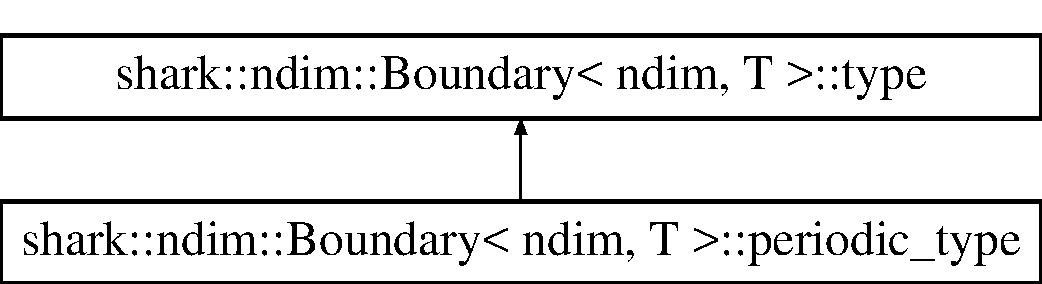
\includegraphics[height=2.000000cm]{classshark_1_1ndim_1_1_boundary_1_1periodic__type}
\end{center}
\end{figure}
\subsection*{Public Member Functions}
\begin{DoxyCompactItemize}
\item 
\hyperlink{classshark_1_1ndim_1_1_boundary_1_1periodic__type_a2a2361be7dd3d056049d46160c7dbafa}{periodic\+\_\+type} ()
\item 
virtual \hyperlink{classshark_1_1ndim_1_1_boundary_1_1periodic__type_a0a83253b5e97de76c244b2a971416a19}{$\sim$periodic\+\_\+type} ()
\item 
virtual \hyperlink{classshark_1_1ndim_1_1_boundary_1_1periodic__type}{periodic\+\_\+type} $\ast$ \hyperlink{classshark_1_1ndim_1_1_boundary_1_1periodic__type_a54904c3d305d26abe8cc8f4b85d9d7e0}{clone} () const
\end{DoxyCompactItemize}


\subsection{Detailed Description}
\subsubsection*{template$<$int ndim, typename T$>$\newline
class shark\+::ndim\+::\+Boundary$<$ ndim, T $>$\+::periodic\+\_\+type}



Definition at line 35 of file boundary.\+hpp.



\subsection{Constructor \& Destructor Documentation}
\hypertarget{classshark_1_1ndim_1_1_boundary_1_1periodic__type_a2a2361be7dd3d056049d46160c7dbafa}{}\label{classshark_1_1ndim_1_1_boundary_1_1periodic__type_a2a2361be7dd3d056049d46160c7dbafa} 
\index{shark\+::ndim\+::\+Boundary\+::periodic\+\_\+type@{shark\+::ndim\+::\+Boundary\+::periodic\+\_\+type}!periodic\+\_\+type@{periodic\+\_\+type}}
\index{periodic\+\_\+type@{periodic\+\_\+type}!shark\+::ndim\+::\+Boundary\+::periodic\+\_\+type@{shark\+::ndim\+::\+Boundary\+::periodic\+\_\+type}}
\subsubsection{\texorpdfstring{periodic\+\_\+type()}{periodic\_type()}}
{\footnotesize\ttfamily template$<$int ndim, typename T $>$ \\
Boundary\+::periodic\+\_\+type\+::periodic\+\_\+type (\begin{DoxyParamCaption}{ }\end{DoxyParamCaption})}



Definition at line 22 of file boundary.\+cpp.


\begin{DoxyCode}
22 \{ \}
\end{DoxyCode}
\hypertarget{classshark_1_1ndim_1_1_boundary_1_1periodic__type_a0a83253b5e97de76c244b2a971416a19}{}\label{classshark_1_1ndim_1_1_boundary_1_1periodic__type_a0a83253b5e97de76c244b2a971416a19} 
\index{shark\+::ndim\+::\+Boundary\+::periodic\+\_\+type@{shark\+::ndim\+::\+Boundary\+::periodic\+\_\+type}!````~periodic\+\_\+type@{$\sim$periodic\+\_\+type}}
\index{````~periodic\+\_\+type@{$\sim$periodic\+\_\+type}!shark\+::ndim\+::\+Boundary\+::periodic\+\_\+type@{shark\+::ndim\+::\+Boundary\+::periodic\+\_\+type}}
\subsubsection{\texorpdfstring{$\sim$periodic\+\_\+type()}{~periodic\_type()}}
{\footnotesize\ttfamily template$<$int ndim, typename T $>$ \\
Boundary\+::periodic\+\_\+type\+::$\sim$periodic\+\_\+type (\begin{DoxyParamCaption}{ }\end{DoxyParamCaption})\hspace{0.3cm}{\ttfamily [virtual]}}



Definition at line 25 of file boundary.\+cpp.


\begin{DoxyCode}
25 \{ \}
\end{DoxyCode}


\subsection{Member Function Documentation}
\hypertarget{classshark_1_1ndim_1_1_boundary_1_1periodic__type_a54904c3d305d26abe8cc8f4b85d9d7e0}{}\label{classshark_1_1ndim_1_1_boundary_1_1periodic__type_a54904c3d305d26abe8cc8f4b85d9d7e0} 
\index{shark\+::ndim\+::\+Boundary\+::periodic\+\_\+type@{shark\+::ndim\+::\+Boundary\+::periodic\+\_\+type}!clone@{clone}}
\index{clone@{clone}!shark\+::ndim\+::\+Boundary\+::periodic\+\_\+type@{shark\+::ndim\+::\+Boundary\+::periodic\+\_\+type}}
\subsubsection{\texorpdfstring{clone()}{clone()}}
{\footnotesize\ttfamily template$<$int ndim, typename T $>$ \\
\hyperlink{classshark_1_1ndim_1_1_boundary}{Boundary}$<$ ndim, T $>$\+::\hyperlink{classshark_1_1ndim_1_1_boundary_1_1periodic__type}{periodic\+\_\+type} $\ast$ Boundary\+::periodic\+\_\+type\+::clone (\begin{DoxyParamCaption}{ }\end{DoxyParamCaption}) const\hspace{0.3cm}{\ttfamily [virtual]}}



Reimplemented from \hyperlink{classshark_1_1ndim_1_1_boundary_1_1type_a5651988ce3a6c229009d3fa849e820dc}{shark\+::ndim\+::\+Boundary$<$ ndim, T $>$\+::type}.



Definition at line 28 of file boundary.\+cpp.


\begin{DoxyCode}
28                                                                                    \{
29     \textcolor{keywordflow}{return} \textcolor{keyword}{new} \hyperlink{classshark_1_1ndim_1_1_boundary_1_1periodic__type_a2a2361be7dd3d056049d46160c7dbafa}{periodic\_type}();
30 \}
\end{DoxyCode}


The documentation for this class was generated from the following files\+:\begin{DoxyCompactItemize}
\item 
include/shark/\hyperlink{boundary_8hpp}{boundary.\+hpp}\item 
src/\hyperlink{boundary_8cpp}{boundary.\+cpp}\end{DoxyCompactItemize}

\hypertarget{classshark_1_1ndim_1_1_periodic_shift}{}\section{shark\+:\+:ndim\+:\+:Periodic\+Shift$<$ ndim, S $>$ Class Template Reference}
\label{classshark_1_1ndim_1_1_periodic_shift}\index{shark\+::ndim\+::\+Periodic\+Shift$<$ ndim, S $>$@{shark\+::ndim\+::\+Periodic\+Shift$<$ ndim, S $>$}}


{\ttfamily \#include $<$expr.\+hpp$>$}

\subsection*{Public Member Functions}
\begin{DoxyCompactItemize}
\item 
\hyperlink{classshark_1_1ndim_1_1_periodic_shift_aceef16e1e0671276f46277d219386d68}{Periodic\+Shift} (\hyperlink{structshark_1_1ndim_1_1coords__range}{coords\+\_\+range}$<$ ndim $>$ \hyperlink{classshark_1_1ndim_1_1_periodic_shift_ad2b058280d2b466c8acb82e6f473e240}{r}, \hyperlink{structshark_1_1ndim_1_1coords}{coords}$<$ ndim $>$ \hyperlink{classshark_1_1ndim_1_1_periodic_shift_aded04c5bc0760cfb247590c85921b653}{sw})
\item 
auto \hyperlink{classshark_1_1ndim_1_1_periodic_shift_acc2d3268c34e15655301843e4370a349}{operator()} (const typename S\+::accessor \&a, \hyperlink{structshark_1_1ndim_1_1coords}{coords}$<$ ndim $>$ ii) const -\/$>$ decltype(a(ii))
\end{DoxyCompactItemize}
\subsection*{Private Attributes}
\begin{DoxyCompactItemize}
\item 
\hyperlink{structshark_1_1ndim_1_1coords__range}{coords\+\_\+range}$<$ ndim $>$ \hyperlink{classshark_1_1ndim_1_1_periodic_shift_ad2b058280d2b466c8acb82e6f473e240}{r}
\item 
\hyperlink{structshark_1_1ndim_1_1coords}{coords}$<$ ndim $>$ \hyperlink{classshark_1_1ndim_1_1_periodic_shift_aded04c5bc0760cfb247590c85921b653}{sw}
\end{DoxyCompactItemize}


\subsection{Detailed Description}
\subsubsection*{template$<$int ndim, typename S$>$\newline
class shark\+::ndim\+::\+Periodic\+Shift$<$ ndim, S $>$}



Definition at line 671 of file expr.\+hpp.



\subsection{Constructor \& Destructor Documentation}
\hypertarget{classshark_1_1ndim_1_1_periodic_shift_aceef16e1e0671276f46277d219386d68}{}\label{classshark_1_1ndim_1_1_periodic_shift_aceef16e1e0671276f46277d219386d68} 
\index{shark\+::ndim\+::\+Periodic\+Shift@{shark\+::ndim\+::\+Periodic\+Shift}!Periodic\+Shift@{Periodic\+Shift}}
\index{Periodic\+Shift@{Periodic\+Shift}!shark\+::ndim\+::\+Periodic\+Shift@{shark\+::ndim\+::\+Periodic\+Shift}}
\subsubsection{\texorpdfstring{Periodic\+Shift()}{PeriodicShift()}}
{\footnotesize\ttfamily template$<$int ndim, typename S $>$ \\
\hyperlink{classshark_1_1ndim_1_1_periodic_shift}{shark\+::ndim\+::\+Periodic\+Shift}$<$ ndim, S $>$\+::\hyperlink{classshark_1_1ndim_1_1_periodic_shift}{Periodic\+Shift} (\begin{DoxyParamCaption}\item[{\hyperlink{structshark_1_1ndim_1_1coords__range}{coords\+\_\+range}$<$ ndim $>$}]{r,  }\item[{\hyperlink{structshark_1_1ndim_1_1coords}{coords}$<$ ndim $>$}]{sw }\end{DoxyParamCaption})}



Definition at line 682 of file expr.\+hpp.


\begin{DoxyCode}
682 : \hyperlink{classshark_1_1ndim_1_1_periodic_shift_ad2b058280d2b466c8acb82e6f473e240}{r}(\hyperlink{classshark_1_1ndim_1_1_periodic_shift_ad2b058280d2b466c8acb82e6f473e240}{r}), \hyperlink{classshark_1_1ndim_1_1_periodic_shift_aded04c5bc0760cfb247590c85921b653}{sw}(\hyperlink{classshark_1_1ndim_1_1_periodic_shift_aded04c5bc0760cfb247590c85921b653}{sw}) \{ \}
\end{DoxyCode}


\subsection{Member Function Documentation}
\hypertarget{classshark_1_1ndim_1_1_periodic_shift_acc2d3268c34e15655301843e4370a349}{}\label{classshark_1_1ndim_1_1_periodic_shift_acc2d3268c34e15655301843e4370a349} 
\index{shark\+::ndim\+::\+Periodic\+Shift@{shark\+::ndim\+::\+Periodic\+Shift}!operator()@{operator()}}
\index{operator()@{operator()}!shark\+::ndim\+::\+Periodic\+Shift@{shark\+::ndim\+::\+Periodic\+Shift}}
\subsubsection{\texorpdfstring{operator()()}{operator()()}}
{\footnotesize\ttfamily template$<$int ndim, typename S $>$ \\
auto \hyperlink{classshark_1_1ndim_1_1_periodic_shift}{shark\+::ndim\+::\+Periodic\+Shift}$<$ ndim, S $>$\+::operator() (\begin{DoxyParamCaption}\item[{const typename S\+::accessor \&}]{a,  }\item[{\hyperlink{structshark_1_1ndim_1_1coords}{coords}$<$ ndim $>$}]{ii }\end{DoxyParamCaption}) const -\/$>$ decltype(a(ii)) \hspace{0.3cm}{\ttfamily [inline]}}



Definition at line 676 of file expr.\+hpp.


\begin{DoxyCode}
676                                                                                                    \{
677                 \textcolor{keywordflow}{return} a(\hyperlink{classshark_1_1ndim_1_1_periodic_shift_ad2b058280d2b466c8acb82e6f473e240}{r}.periodic\_equiv(ii+\hyperlink{classshark_1_1ndim_1_1_periodic_shift_aded04c5bc0760cfb247590c85921b653}{sw}));
678             \}
\end{DoxyCode}


\subsection{Member Data Documentation}
\hypertarget{classshark_1_1ndim_1_1_periodic_shift_ad2b058280d2b466c8acb82e6f473e240}{}\label{classshark_1_1ndim_1_1_periodic_shift_ad2b058280d2b466c8acb82e6f473e240} 
\index{shark\+::ndim\+::\+Periodic\+Shift@{shark\+::ndim\+::\+Periodic\+Shift}!r@{r}}
\index{r@{r}!shark\+::ndim\+::\+Periodic\+Shift@{shark\+::ndim\+::\+Periodic\+Shift}}
\subsubsection{\texorpdfstring{r}{r}}
{\footnotesize\ttfamily template$<$int ndim, typename S $>$ \\
\hyperlink{structshark_1_1ndim_1_1coords__range}{coords\+\_\+range}$<$ndim$>$ \hyperlink{classshark_1_1ndim_1_1_periodic_shift}{shark\+::ndim\+::\+Periodic\+Shift}$<$ ndim, S $>$\+::r\hspace{0.3cm}{\ttfamily [private]}}



Definition at line 672 of file expr.\+hpp.

\hypertarget{classshark_1_1ndim_1_1_periodic_shift_aded04c5bc0760cfb247590c85921b653}{}\label{classshark_1_1ndim_1_1_periodic_shift_aded04c5bc0760cfb247590c85921b653} 
\index{shark\+::ndim\+::\+Periodic\+Shift@{shark\+::ndim\+::\+Periodic\+Shift}!sw@{sw}}
\index{sw@{sw}!shark\+::ndim\+::\+Periodic\+Shift@{shark\+::ndim\+::\+Periodic\+Shift}}
\subsubsection{\texorpdfstring{sw}{sw}}
{\footnotesize\ttfamily template$<$int ndim, typename S $>$ \\
\hyperlink{structshark_1_1ndim_1_1coords}{coords}$<$ndim$>$ \hyperlink{classshark_1_1ndim_1_1_periodic_shift}{shark\+::ndim\+::\+Periodic\+Shift}$<$ ndim, S $>$\+::sw\hspace{0.3cm}{\ttfamily [private]}}



Definition at line 673 of file expr.\+hpp.



The documentation for this class was generated from the following file\+:\begin{DoxyCompactItemize}
\item 
include/shark/\hyperlink{expr_8hpp}{expr.\+hpp}\end{DoxyCompactItemize}

\hypertarget{classshark_1_1ndim_1_1_domain_1_1_process_overlap}{}\section{shark\+:\+:ndim\+:\+:Domain$<$ ndim $>$\+:\+:Process\+Overlap Class Reference}
\label{classshark_1_1ndim_1_1_domain_1_1_process_overlap}\index{shark\+::ndim\+::\+Domain$<$ ndim $>$\+::\+Process\+Overlap@{shark\+::ndim\+::\+Domain$<$ ndim $>$\+::\+Process\+Overlap}}


{\ttfamily \#include $<$domain.\+hpp$>$}

\subsection*{Private Attributes}
\begin{DoxyCompactItemize}
\item 
const \hyperlink{classshark_1_1ndim_1_1_domain}{Domain}$<$ ndim $>$ \& \hyperlink{classshark_1_1ndim_1_1_domain_1_1_process_overlap_af73890c5892d8071cdfb29e66ae4e8d8}{dom}
\item 
const \hyperlink{structshark_1_1ndim_1_1coords__range}{coords\+\_\+range}$<$ ndim $>$ \hyperlink{classshark_1_1ndim_1_1_domain_1_1_process_overlap_a1130b73407bf2aaa0a8cb6ac25fcb3c1}{range}
\item 
\hyperlink{classshark_1_1ndim_1_1_domain_a9684ccd8af33cff7639c782290ac37ee}{pcoords} \hyperlink{classshark_1_1ndim_1_1_domain_1_1_process_overlap_ad2db26b8b1a91fd5dea72ffe01a2ac78}{lip}
\item 
\hyperlink{classshark_1_1ndim_1_1_domain_a9684ccd8af33cff7639c782290ac37ee}{pcoords} \hyperlink{classshark_1_1ndim_1_1_domain_1_1_process_overlap_acf20a1ff561cd7b0f50f8f6983cc6283}{uip}
\item 
\hyperlink{structshark_1_1ndim_1_1coords}{coords}$<$ ndim $>$ \hyperlink{classshark_1_1ndim_1_1_domain_1_1_process_overlap_aedfe1a1b3943d517faa3203f201bbc10}{loff}
\item 
\hyperlink{structshark_1_1ndim_1_1coords}{coords}$<$ ndim $>$ \hyperlink{classshark_1_1ndim_1_1_domain_1_1_process_overlap_a9c5f411b46b6a0c7ffab30b43898371e}{uoff}
\end{DoxyCompactItemize}


\subsection{Detailed Description}
\subsubsection*{template$<$int ndim$>$\newline
class shark\+::ndim\+::\+Domain$<$ ndim $>$\+::\+Process\+Overlap}



Definition at line 267 of file domain.\+hpp.



\subsection{Member Data Documentation}
\hypertarget{classshark_1_1ndim_1_1_domain_1_1_process_overlap_af73890c5892d8071cdfb29e66ae4e8d8}{}\label{classshark_1_1ndim_1_1_domain_1_1_process_overlap_af73890c5892d8071cdfb29e66ae4e8d8} 
\index{shark\+::ndim\+::\+Domain\+::\+Process\+Overlap@{shark\+::ndim\+::\+Domain\+::\+Process\+Overlap}!dom@{dom}}
\index{dom@{dom}!shark\+::ndim\+::\+Domain\+::\+Process\+Overlap@{shark\+::ndim\+::\+Domain\+::\+Process\+Overlap}}
\subsubsection{\texorpdfstring{dom}{dom}}
{\footnotesize\ttfamily template$<$int ndim$>$ \\
const \hyperlink{classshark_1_1ndim_1_1_domain}{Domain}$<$ndim$>$\& \hyperlink{classshark_1_1ndim_1_1_domain}{shark\+::ndim\+::\+Domain}$<$ ndim $>$\+::Process\+Overlap\+::dom\hspace{0.3cm}{\ttfamily [private]}}



Definition at line 268 of file domain.\+hpp.

\hypertarget{classshark_1_1ndim_1_1_domain_1_1_process_overlap_ad2db26b8b1a91fd5dea72ffe01a2ac78}{}\label{classshark_1_1ndim_1_1_domain_1_1_process_overlap_ad2db26b8b1a91fd5dea72ffe01a2ac78} 
\index{shark\+::ndim\+::\+Domain\+::\+Process\+Overlap@{shark\+::ndim\+::\+Domain\+::\+Process\+Overlap}!lip@{lip}}
\index{lip@{lip}!shark\+::ndim\+::\+Domain\+::\+Process\+Overlap@{shark\+::ndim\+::\+Domain\+::\+Process\+Overlap}}
\subsubsection{\texorpdfstring{lip}{lip}}
{\footnotesize\ttfamily template$<$int ndim$>$ \\
\hyperlink{classshark_1_1ndim_1_1_domain_a9684ccd8af33cff7639c782290ac37ee}{pcoords} \hyperlink{classshark_1_1ndim_1_1_domain}{shark\+::ndim\+::\+Domain}$<$ ndim $>$\+::Process\+Overlap\+::lip\hspace{0.3cm}{\ttfamily [private]}}



Definition at line 271 of file domain.\+hpp.

\hypertarget{classshark_1_1ndim_1_1_domain_1_1_process_overlap_aedfe1a1b3943d517faa3203f201bbc10}{}\label{classshark_1_1ndim_1_1_domain_1_1_process_overlap_aedfe1a1b3943d517faa3203f201bbc10} 
\index{shark\+::ndim\+::\+Domain\+::\+Process\+Overlap@{shark\+::ndim\+::\+Domain\+::\+Process\+Overlap}!loff@{loff}}
\index{loff@{loff}!shark\+::ndim\+::\+Domain\+::\+Process\+Overlap@{shark\+::ndim\+::\+Domain\+::\+Process\+Overlap}}
\subsubsection{\texorpdfstring{loff}{loff}}
{\footnotesize\ttfamily template$<$int ndim$>$ \\
\hyperlink{structshark_1_1ndim_1_1coords}{coords}$<$ndim$>$ \hyperlink{classshark_1_1ndim_1_1_domain}{shark\+::ndim\+::\+Domain}$<$ ndim $>$\+::Process\+Overlap\+::loff\hspace{0.3cm}{\ttfamily [private]}}



Definition at line 272 of file domain.\+hpp.

\hypertarget{classshark_1_1ndim_1_1_domain_1_1_process_overlap_a1130b73407bf2aaa0a8cb6ac25fcb3c1}{}\label{classshark_1_1ndim_1_1_domain_1_1_process_overlap_a1130b73407bf2aaa0a8cb6ac25fcb3c1} 
\index{shark\+::ndim\+::\+Domain\+::\+Process\+Overlap@{shark\+::ndim\+::\+Domain\+::\+Process\+Overlap}!range@{range}}
\index{range@{range}!shark\+::ndim\+::\+Domain\+::\+Process\+Overlap@{shark\+::ndim\+::\+Domain\+::\+Process\+Overlap}}
\subsubsection{\texorpdfstring{range}{range}}
{\footnotesize\ttfamily template$<$int ndim$>$ \\
const \hyperlink{structshark_1_1ndim_1_1coords__range}{coords\+\_\+range}$<$ndim$>$ \hyperlink{classshark_1_1ndim_1_1_domain}{shark\+::ndim\+::\+Domain}$<$ ndim $>$\+::Process\+Overlap\+::range\hspace{0.3cm}{\ttfamily [private]}}



Definition at line 269 of file domain.\+hpp.

\hypertarget{classshark_1_1ndim_1_1_domain_1_1_process_overlap_acf20a1ff561cd7b0f50f8f6983cc6283}{}\label{classshark_1_1ndim_1_1_domain_1_1_process_overlap_acf20a1ff561cd7b0f50f8f6983cc6283} 
\index{shark\+::ndim\+::\+Domain\+::\+Process\+Overlap@{shark\+::ndim\+::\+Domain\+::\+Process\+Overlap}!uip@{uip}}
\index{uip@{uip}!shark\+::ndim\+::\+Domain\+::\+Process\+Overlap@{shark\+::ndim\+::\+Domain\+::\+Process\+Overlap}}
\subsubsection{\texorpdfstring{uip}{uip}}
{\footnotesize\ttfamily template$<$int ndim$>$ \\
\hyperlink{classshark_1_1ndim_1_1_domain_a9684ccd8af33cff7639c782290ac37ee}{pcoords} \hyperlink{classshark_1_1ndim_1_1_domain}{shark\+::ndim\+::\+Domain}$<$ ndim $>$\+::Process\+Overlap\+::uip\hspace{0.3cm}{\ttfamily [private]}}



Definition at line 271 of file domain.\+hpp.

\hypertarget{classshark_1_1ndim_1_1_domain_1_1_process_overlap_a9c5f411b46b6a0c7ffab30b43898371e}{}\label{classshark_1_1ndim_1_1_domain_1_1_process_overlap_a9c5f411b46b6a0c7ffab30b43898371e} 
\index{shark\+::ndim\+::\+Domain\+::\+Process\+Overlap@{shark\+::ndim\+::\+Domain\+::\+Process\+Overlap}!uoff@{uoff}}
\index{uoff@{uoff}!shark\+::ndim\+::\+Domain\+::\+Process\+Overlap@{shark\+::ndim\+::\+Domain\+::\+Process\+Overlap}}
\subsubsection{\texorpdfstring{uoff}{uoff}}
{\footnotesize\ttfamily template$<$int ndim$>$ \\
\hyperlink{structshark_1_1ndim_1_1coords}{coords}$<$ndim$>$ \hyperlink{classshark_1_1ndim_1_1_domain}{shark\+::ndim\+::\+Domain}$<$ ndim $>$\+::Process\+Overlap\+::uoff\hspace{0.3cm}{\ttfamily [private]}}



Definition at line 272 of file domain.\+hpp.



The documentation for this class was generated from the following file\+:\begin{DoxyCompactItemize}
\item 
include/shark/\hyperlink{domain_8hpp}{domain.\+hpp}\end{DoxyCompactItemize}

\hypertarget{classshark_1_1_request_q}{}\section{shark\+:\+:RequestQ$<$ typename, typename $>$ Class Template Reference}
\label{classshark_1_1_request_q}\index{shark\+::\+Request\+Q$<$ typename, typename $>$@{shark\+::\+Request\+Q$<$ typename, typename $>$}}


{\ttfamily \#include $<$common.\+hpp$>$}



\subsection{Detailed Description}
\subsubsection*{template$<$typename, typename$>$\newline
class shark\+::\+Request\+Q$<$ typename, typename $>$}



Definition at line 150 of file common.\+hpp.



The documentation for this class was generated from the following file\+:\begin{DoxyCompactItemize}
\item 
include/shark/\hyperlink{common_8hpp}{common.\+hpp}\end{DoxyCompactItemize}

\hypertarget{classshark_1_1ndim_1_1_s_coord_val}{}\section{shark\+:\+:ndim\+:\+:S\+Coord\+Val$<$ d, ndim, T $>$ Class Template Reference}
\label{classshark_1_1ndim_1_1_s_coord_val}\index{shark\+::ndim\+::\+S\+Coord\+Val$<$ d, ndim, T $>$@{shark\+::ndim\+::\+S\+Coord\+Val$<$ d, ndim, T $>$}}


{\ttfamily \#include $<$expr.\+hpp$>$}

\subsection*{Public Member Functions}
\begin{DoxyCompactItemize}
\item 
\hyperlink{classshark_1_1ndim_1_1_s_coord_val_affad44c0ca1502ee2c63dd555a84a4ab}{S\+Coord\+Val} (\hyperlink{namespaceshark_a767a92d5dd82cb82266473bff42fa6d9}{coord} \hyperlink{classshark_1_1ndim_1_1_s_coord_val_a11ff11a433e0b0cfb8b5de96b3583eb2}{lower}, T \hyperlink{classshark_1_1ndim_1_1_s_coord_val_afd74ad2086b0e8c5bab9ee5906ec08fa}{step})
\item 
\hyperlink{classshark_1_1ndim_1_1_s_coord_val_aac1792753976c8339c7430550fd88bea}{$\sim$\+S\+Coord\+Val} ()
\item 
\hyperlink{common_8hpp_a2eb6f9e0395b47b8d5e3eeae4fe0c116}{I\+N\+L\+I\+NE} T \hyperlink{classshark_1_1ndim_1_1_s_coord_val_a6f32f75d306418cd9ac4392f058f1db6}{operator()} (\hyperlink{structshark_1_1ndim_1_1coords}{coords}$<$ ndim $>$ ii) const
\end{DoxyCompactItemize}
\subsection*{Private Attributes}
\begin{DoxyCompactItemize}
\item 
const \hyperlink{namespaceshark_a767a92d5dd82cb82266473bff42fa6d9}{coord} \hyperlink{classshark_1_1ndim_1_1_s_coord_val_a11ff11a433e0b0cfb8b5de96b3583eb2}{lower}
\item 
const T \hyperlink{classshark_1_1ndim_1_1_s_coord_val_afd74ad2086b0e8c5bab9ee5906ec08fa}{step}
\end{DoxyCompactItemize}


\subsection{Detailed Description}
\subsubsection*{template$<$int d, int ndim, typename T$>$\newline
class shark\+::ndim\+::\+S\+Coord\+Val$<$ d, ndim, T $>$}



Definition at line 506 of file expr.\+hpp.



\subsection{Constructor \& Destructor Documentation}
\hypertarget{classshark_1_1ndim_1_1_s_coord_val_affad44c0ca1502ee2c63dd555a84a4ab}{}\label{classshark_1_1ndim_1_1_s_coord_val_affad44c0ca1502ee2c63dd555a84a4ab} 
\index{shark\+::ndim\+::\+S\+Coord\+Val@{shark\+::ndim\+::\+S\+Coord\+Val}!S\+Coord\+Val@{S\+Coord\+Val}}
\index{S\+Coord\+Val@{S\+Coord\+Val}!shark\+::ndim\+::\+S\+Coord\+Val@{shark\+::ndim\+::\+S\+Coord\+Val}}
\subsubsection{\texorpdfstring{S\+Coord\+Val()}{SCoordVal()}}
{\footnotesize\ttfamily template$<$int d, int ndim, typename T $>$ \\
\hyperlink{classshark_1_1ndim_1_1_s_coord_val}{shark\+::ndim\+::\+S\+Coord\+Val}$<$ d, ndim, T $>$\+::\hyperlink{classshark_1_1ndim_1_1_s_coord_val}{S\+Coord\+Val} (\begin{DoxyParamCaption}\item[{\hyperlink{namespaceshark_a767a92d5dd82cb82266473bff42fa6d9}{coord}}]{lower,  }\item[{T}]{step }\end{DoxyParamCaption})}



Definition at line 522 of file expr.\+hpp.


\begin{DoxyCode}
522 : \hyperlink{classshark_1_1ndim_1_1_s_coord_val_a11ff11a433e0b0cfb8b5de96b3583eb2}{lower}(\hyperlink{classshark_1_1ndim_1_1_s_coord_val_a11ff11a433e0b0cfb8b5de96b3583eb2}{lower}), \hyperlink{classshark_1_1ndim_1_1_s_coord_val_afd74ad2086b0e8c5bab9ee5906ec08fa}{step}(\hyperlink{classshark_1_1ndim_1_1_s_coord_val_afd74ad2086b0e8c5bab9ee5906ec08fa}{step}) \{ \}
\end{DoxyCode}
\hypertarget{classshark_1_1ndim_1_1_s_coord_val_aac1792753976c8339c7430550fd88bea}{}\label{classshark_1_1ndim_1_1_s_coord_val_aac1792753976c8339c7430550fd88bea} 
\index{shark\+::ndim\+::\+S\+Coord\+Val@{shark\+::ndim\+::\+S\+Coord\+Val}!````~S\+Coord\+Val@{$\sim$\+S\+Coord\+Val}}
\index{````~S\+Coord\+Val@{$\sim$\+S\+Coord\+Val}!shark\+::ndim\+::\+S\+Coord\+Val@{shark\+::ndim\+::\+S\+Coord\+Val}}
\subsubsection{\texorpdfstring{$\sim$\+S\+Coord\+Val()}{~SCoordVal()}}
{\footnotesize\ttfamily template$<$int d, int ndim, typename T $>$ \\
\hyperlink{classshark_1_1ndim_1_1_s_coord_val}{shark\+::ndim\+::\+S\+Coord\+Val}$<$ d, ndim, T $>$\+::$\sim$\hyperlink{classshark_1_1ndim_1_1_s_coord_val}{S\+Coord\+Val} (\begin{DoxyParamCaption}{ }\end{DoxyParamCaption})}



Definition at line 525 of file expr.\+hpp.


\begin{DoxyCode}
525 \{ \}
\end{DoxyCode}


\subsection{Member Function Documentation}
\hypertarget{classshark_1_1ndim_1_1_s_coord_val_a6f32f75d306418cd9ac4392f058f1db6}{}\label{classshark_1_1ndim_1_1_s_coord_val_a6f32f75d306418cd9ac4392f058f1db6} 
\index{shark\+::ndim\+::\+S\+Coord\+Val@{shark\+::ndim\+::\+S\+Coord\+Val}!operator()@{operator()}}
\index{operator()@{operator()}!shark\+::ndim\+::\+S\+Coord\+Val@{shark\+::ndim\+::\+S\+Coord\+Val}}
\subsubsection{\texorpdfstring{operator()()}{operator()()}}
{\footnotesize\ttfamily template$<$int d, int ndim, typename T $>$ \\
T \hyperlink{classshark_1_1ndim_1_1_s_coord_val}{shark\+::ndim\+::\+S\+Coord\+Val}$<$ d, ndim, T $>$\+::operator() (\begin{DoxyParamCaption}\item[{\hyperlink{structshark_1_1ndim_1_1coords}{coords}$<$ ndim $>$}]{ii }\end{DoxyParamCaption}) const\hspace{0.3cm}{\ttfamily [inline]}}



Definition at line 517 of file expr.\+hpp.


\begin{DoxyCode}
517                                                                       \{
518             \textcolor{keywordflow}{return} (ii[d] - \hyperlink{classshark_1_1ndim_1_1_s_coord_val_a11ff11a433e0b0cfb8b5de96b3583eb2}{lower}) * \hyperlink{classshark_1_1ndim_1_1_s_coord_val_afd74ad2086b0e8c5bab9ee5906ec08fa}{step};
519         \}
\end{DoxyCode}


\subsection{Member Data Documentation}
\hypertarget{classshark_1_1ndim_1_1_s_coord_val_a11ff11a433e0b0cfb8b5de96b3583eb2}{}\label{classshark_1_1ndim_1_1_s_coord_val_a11ff11a433e0b0cfb8b5de96b3583eb2} 
\index{shark\+::ndim\+::\+S\+Coord\+Val@{shark\+::ndim\+::\+S\+Coord\+Val}!lower@{lower}}
\index{lower@{lower}!shark\+::ndim\+::\+S\+Coord\+Val@{shark\+::ndim\+::\+S\+Coord\+Val}}
\subsubsection{\texorpdfstring{lower}{lower}}
{\footnotesize\ttfamily template$<$int d, int ndim, typename T $>$ \\
const \hyperlink{namespaceshark_a767a92d5dd82cb82266473bff42fa6d9}{coord} \hyperlink{classshark_1_1ndim_1_1_s_coord_val}{shark\+::ndim\+::\+S\+Coord\+Val}$<$ d, ndim, T $>$\+::lower\hspace{0.3cm}{\ttfamily [private]}}



Definition at line 507 of file expr.\+hpp.

\hypertarget{classshark_1_1ndim_1_1_s_coord_val_afd74ad2086b0e8c5bab9ee5906ec08fa}{}\label{classshark_1_1ndim_1_1_s_coord_val_afd74ad2086b0e8c5bab9ee5906ec08fa} 
\index{shark\+::ndim\+::\+S\+Coord\+Val@{shark\+::ndim\+::\+S\+Coord\+Val}!step@{step}}
\index{step@{step}!shark\+::ndim\+::\+S\+Coord\+Val@{shark\+::ndim\+::\+S\+Coord\+Val}}
\subsubsection{\texorpdfstring{step}{step}}
{\footnotesize\ttfamily template$<$int d, int ndim, typename T $>$ \\
const T \hyperlink{classshark_1_1ndim_1_1_s_coord_val}{shark\+::ndim\+::\+S\+Coord\+Val}$<$ d, ndim, T $>$\+::step\hspace{0.3cm}{\ttfamily [private]}}



Definition at line 508 of file expr.\+hpp.



The documentation for this class was generated from the following file\+:\begin{DoxyCompactItemize}
\item 
include/shark/\hyperlink{expr_8hpp}{expr.\+hpp}\end{DoxyCompactItemize}

\hypertarget{classshark_1_1ndim_1_1_s_coord_vec}{}\section{shark\+:\+:ndim\+:\+:S\+Coord\+Vec$<$ ndim, T $>$ Class Template Reference}
\label{classshark_1_1ndim_1_1_s_coord_vec}\index{shark\+::ndim\+::\+S\+Coord\+Vec$<$ ndim, T $>$@{shark\+::ndim\+::\+S\+Coord\+Vec$<$ ndim, T $>$}}


{\ttfamily \#include $<$expr.\+hpp$>$}

\subsection*{Public Member Functions}
\begin{DoxyCompactItemize}
\item 
\hyperlink{classshark_1_1ndim_1_1_s_coord_vec_a2206234f04728b090829ce9cdb3d0be1}{S\+Coord\+Vec} (\hyperlink{structshark_1_1ndim_1_1coords}{coords}$<$ ndim $>$ \hyperlink{classshark_1_1ndim_1_1_s_coord_vec_aec6b26f59abee649139be7a517101d04}{lower}, \hyperlink{structshark_1_1ndim_1_1vec}{vec}$<$ ndim, T $>$ \hyperlink{classshark_1_1ndim_1_1_s_coord_vec_aa2ce747ed08501f5fe6bf4a8c6b25a20}{step})
\item 
\hyperlink{classshark_1_1ndim_1_1_s_coord_vec_a965693ba29b2ccd952552ea6cd1c5f3e}{$\sim$\+S\+Coord\+Vec} ()
\item 
\hyperlink{common_8hpp_a2eb6f9e0395b47b8d5e3eeae4fe0c116}{I\+N\+L\+I\+NE} \hyperlink{structshark_1_1ndim_1_1vec}{vec}$<$ ndim, T $>$ \hyperlink{classshark_1_1ndim_1_1_s_coord_vec_abad6eb3a4c0fdd994227b8beeee7f86a}{operator()} (\hyperlink{structshark_1_1ndim_1_1coords}{coords}$<$ ndim $>$ ii) const
\end{DoxyCompactItemize}
\subsection*{Private Attributes}
\begin{DoxyCompactItemize}
\item 
const \hyperlink{structshark_1_1ndim_1_1coords}{coords}$<$ ndim $>$ \hyperlink{classshark_1_1ndim_1_1_s_coord_vec_aec6b26f59abee649139be7a517101d04}{lower}
\item 
const \hyperlink{structshark_1_1ndim_1_1vec}{vec}$<$ ndim, T $>$ \hyperlink{classshark_1_1ndim_1_1_s_coord_vec_aa2ce747ed08501f5fe6bf4a8c6b25a20}{step}
\end{DoxyCompactItemize}


\subsection{Detailed Description}
\subsubsection*{template$<$int ndim, typename T$>$\newline
class shark\+::ndim\+::\+S\+Coord\+Vec$<$ ndim, T $>$}



Definition at line 458 of file expr.\+hpp.



\subsection{Constructor \& Destructor Documentation}
\hypertarget{classshark_1_1ndim_1_1_s_coord_vec_a2206234f04728b090829ce9cdb3d0be1}{}\label{classshark_1_1ndim_1_1_s_coord_vec_a2206234f04728b090829ce9cdb3d0be1} 
\index{shark\+::ndim\+::\+S\+Coord\+Vec@{shark\+::ndim\+::\+S\+Coord\+Vec}!S\+Coord\+Vec@{S\+Coord\+Vec}}
\index{S\+Coord\+Vec@{S\+Coord\+Vec}!shark\+::ndim\+::\+S\+Coord\+Vec@{shark\+::ndim\+::\+S\+Coord\+Vec}}
\subsubsection{\texorpdfstring{S\+Coord\+Vec()}{SCoordVec()}}
{\footnotesize\ttfamily template$<$int ndim, typename T $>$ \\
\hyperlink{classshark_1_1ndim_1_1_s_coord_vec}{shark\+::ndim\+::\+S\+Coord\+Vec}$<$ ndim, T $>$\+::\hyperlink{classshark_1_1ndim_1_1_s_coord_vec}{S\+Coord\+Vec} (\begin{DoxyParamCaption}\item[{\hyperlink{structshark_1_1ndim_1_1coords}{coords}$<$ ndim $>$}]{lower,  }\item[{\hyperlink{structshark_1_1ndim_1_1vec}{vec}$<$ ndim, T $>$}]{step }\end{DoxyParamCaption})}



Definition at line 473 of file expr.\+hpp.


\begin{DoxyCode}
473 : \hyperlink{classshark_1_1ndim_1_1_s_coord_vec_aec6b26f59abee649139be7a517101d04}{lower}(\hyperlink{classshark_1_1ndim_1_1_s_coord_vec_aec6b26f59abee649139be7a517101d04}{lower}), \hyperlink{classshark_1_1ndim_1_1_s_coord_vec_aa2ce747ed08501f5fe6bf4a8c6b25a20}{step}(\hyperlink{classshark_1_1ndim_1_1_s_coord_vec_aa2ce747ed08501f5fe6bf4a8c6b25a20}{step}) \{ \}
\end{DoxyCode}
\hypertarget{classshark_1_1ndim_1_1_s_coord_vec_a965693ba29b2ccd952552ea6cd1c5f3e}{}\label{classshark_1_1ndim_1_1_s_coord_vec_a965693ba29b2ccd952552ea6cd1c5f3e} 
\index{shark\+::ndim\+::\+S\+Coord\+Vec@{shark\+::ndim\+::\+S\+Coord\+Vec}!````~S\+Coord\+Vec@{$\sim$\+S\+Coord\+Vec}}
\index{````~S\+Coord\+Vec@{$\sim$\+S\+Coord\+Vec}!shark\+::ndim\+::\+S\+Coord\+Vec@{shark\+::ndim\+::\+S\+Coord\+Vec}}
\subsubsection{\texorpdfstring{$\sim$\+S\+Coord\+Vec()}{~SCoordVec()}}
{\footnotesize\ttfamily template$<$int ndim, typename T $>$ \\
\hyperlink{classshark_1_1ndim_1_1_s_coord_vec}{shark\+::ndim\+::\+S\+Coord\+Vec}$<$ ndim, T $>$\+::$\sim$\hyperlink{classshark_1_1ndim_1_1_s_coord_vec}{S\+Coord\+Vec} (\begin{DoxyParamCaption}{ }\end{DoxyParamCaption})}



Definition at line 476 of file expr.\+hpp.


\begin{DoxyCode}
476 \{ \}
\end{DoxyCode}


\subsection{Member Function Documentation}
\hypertarget{classshark_1_1ndim_1_1_s_coord_vec_abad6eb3a4c0fdd994227b8beeee7f86a}{}\label{classshark_1_1ndim_1_1_s_coord_vec_abad6eb3a4c0fdd994227b8beeee7f86a} 
\index{shark\+::ndim\+::\+S\+Coord\+Vec@{shark\+::ndim\+::\+S\+Coord\+Vec}!operator()@{operator()}}
\index{operator()@{operator()}!shark\+::ndim\+::\+S\+Coord\+Vec@{shark\+::ndim\+::\+S\+Coord\+Vec}}
\subsubsection{\texorpdfstring{operator()()}{operator()()}}
{\footnotesize\ttfamily template$<$int ndim, typename T $>$ \\
\hyperlink{structshark_1_1ndim_1_1vec}{vec}$<$ ndim, T $>$ \hyperlink{classshark_1_1ndim_1_1_s_coord_vec}{shark\+::ndim\+::\+S\+Coord\+Vec}$<$ ndim, T $>$\+::operator() (\begin{DoxyParamCaption}\item[{\hyperlink{structshark_1_1ndim_1_1coords}{coords}$<$ ndim $>$}]{ii }\end{DoxyParamCaption}) const\hspace{0.3cm}{\ttfamily [inline]}}



Definition at line 468 of file expr.\+hpp.


\begin{DoxyCode}
468                                                                               \{
469             \textcolor{keywordflow}{return} (ii - \hyperlink{classshark_1_1ndim_1_1_s_coord_vec_aec6b26f59abee649139be7a517101d04}{lower}).to\_vec() * \hyperlink{classshark_1_1ndim_1_1_s_coord_vec_aa2ce747ed08501f5fe6bf4a8c6b25a20}{step};
470         \}
\end{DoxyCode}


\subsection{Member Data Documentation}
\hypertarget{classshark_1_1ndim_1_1_s_coord_vec_aec6b26f59abee649139be7a517101d04}{}\label{classshark_1_1ndim_1_1_s_coord_vec_aec6b26f59abee649139be7a517101d04} 
\index{shark\+::ndim\+::\+S\+Coord\+Vec@{shark\+::ndim\+::\+S\+Coord\+Vec}!lower@{lower}}
\index{lower@{lower}!shark\+::ndim\+::\+S\+Coord\+Vec@{shark\+::ndim\+::\+S\+Coord\+Vec}}
\subsubsection{\texorpdfstring{lower}{lower}}
{\footnotesize\ttfamily template$<$int ndim, typename T $>$ \\
const \hyperlink{structshark_1_1ndim_1_1coords}{coords}$<$ndim$>$ \hyperlink{classshark_1_1ndim_1_1_s_coord_vec}{shark\+::ndim\+::\+S\+Coord\+Vec}$<$ ndim, T $>$\+::lower\hspace{0.3cm}{\ttfamily [private]}}



Definition at line 459 of file expr.\+hpp.

\hypertarget{classshark_1_1ndim_1_1_s_coord_vec_aa2ce747ed08501f5fe6bf4a8c6b25a20}{}\label{classshark_1_1ndim_1_1_s_coord_vec_aa2ce747ed08501f5fe6bf4a8c6b25a20} 
\index{shark\+::ndim\+::\+S\+Coord\+Vec@{shark\+::ndim\+::\+S\+Coord\+Vec}!step@{step}}
\index{step@{step}!shark\+::ndim\+::\+S\+Coord\+Vec@{shark\+::ndim\+::\+S\+Coord\+Vec}}
\subsubsection{\texorpdfstring{step}{step}}
{\footnotesize\ttfamily template$<$int ndim, typename T $>$ \\
const \hyperlink{structshark_1_1ndim_1_1vec}{vec}$<$ndim,T$>$ \hyperlink{classshark_1_1ndim_1_1_s_coord_vec}{shark\+::ndim\+::\+S\+Coord\+Vec}$<$ ndim, T $>$\+::step\hspace{0.3cm}{\ttfamily [private]}}



Definition at line 460 of file expr.\+hpp.



The documentation for this class was generated from the following file\+:\begin{DoxyCompactItemize}
\item 
include/shark/\hyperlink{expr_8hpp}{expr.\+hpp}\end{DoxyCompactItemize}

\hypertarget{classshark_1_1ndim_1_1_shift}{}\section{shark\+:\+:ndim\+:\+:Shift$<$ S $>$ Class Template Reference}
\label{classshark_1_1ndim_1_1_shift}\index{shark\+::ndim\+::\+Shift$<$ S $>$@{shark\+::ndim\+::\+Shift$<$ S $>$}}


{\ttfamily \#include $<$expr.\+hpp$>$}

\subsection*{Public Member Functions}
\begin{DoxyCompactItemize}
\item 
\hyperlink{classshark_1_1ndim_1_1_shift_adb6138a4655f902116238e4e08e47e68}{Shift} (\hyperlink{structshark_1_1ndim_1_1coords}{coords}$<$ S\+::number\+\_\+of\+\_\+dimensions $>$ \hyperlink{classshark_1_1ndim_1_1_shift_a3bd6f579c282ca70d391bd43bc582331}{sw})
\item 
auto \hyperlink{classshark_1_1ndim_1_1_shift_ac2095531d2a9060eae224166379e4e39}{operator()} (const typename S\+::accessor \&a, \hyperlink{structshark_1_1ndim_1_1coords}{coords}$<$ S\+::number\+\_\+of\+\_\+dimensions $>$ ii) const -\/$>$ decltype(a(ii))
\end{DoxyCompactItemize}
\subsection*{Private Attributes}
\begin{DoxyCompactItemize}
\item 
\hyperlink{structshark_1_1ndim_1_1coords}{coords}$<$ S\+::number\+\_\+of\+\_\+dimensions $>$ \hyperlink{classshark_1_1ndim_1_1_shift_a3bd6f579c282ca70d391bd43bc582331}{sw}
\end{DoxyCompactItemize}


\subsection{Detailed Description}
\subsubsection*{template$<$typename S$>$\newline
class shark\+::ndim\+::\+Shift$<$ S $>$}

\hyperlink{classshark_1_1ndim_1_1_shift}{Shift} 

Definition at line 653 of file expr.\+hpp.



\subsection{Constructor \& Destructor Documentation}
\hypertarget{classshark_1_1ndim_1_1_shift_adb6138a4655f902116238e4e08e47e68}{}\label{classshark_1_1ndim_1_1_shift_adb6138a4655f902116238e4e08e47e68} 
\index{shark\+::ndim\+::\+Shift@{shark\+::ndim\+::\+Shift}!Shift@{Shift}}
\index{Shift@{Shift}!shark\+::ndim\+::\+Shift@{shark\+::ndim\+::\+Shift}}
\subsubsection{\texorpdfstring{Shift()}{Shift()}}
{\footnotesize\ttfamily template$<$typename S $>$ \\
\hyperlink{classshark_1_1ndim_1_1_shift}{shark\+::ndim\+::\+Shift}$<$ S $>$\+::\hyperlink{classshark_1_1ndim_1_1_shift}{Shift} (\begin{DoxyParamCaption}\item[{\hyperlink{structshark_1_1ndim_1_1coords}{coords}$<$ S\+::number\+\_\+of\+\_\+dimensions $>$}]{sw }\end{DoxyParamCaption})}



Definition at line 663 of file expr.\+hpp.


\begin{DoxyCode}
663 : \hyperlink{classshark_1_1ndim_1_1_shift_a3bd6f579c282ca70d391bd43bc582331}{sw}(sw) \{ \}
\end{DoxyCode}


\subsection{Member Function Documentation}
\hypertarget{classshark_1_1ndim_1_1_shift_ac2095531d2a9060eae224166379e4e39}{}\label{classshark_1_1ndim_1_1_shift_ac2095531d2a9060eae224166379e4e39} 
\index{shark\+::ndim\+::\+Shift@{shark\+::ndim\+::\+Shift}!operator()@{operator()}}
\index{operator()@{operator()}!shark\+::ndim\+::\+Shift@{shark\+::ndim\+::\+Shift}}
\subsubsection{\texorpdfstring{operator()()}{operator()()}}
{\footnotesize\ttfamily template$<$typename S $>$ \\
auto \hyperlink{classshark_1_1ndim_1_1_shift}{shark\+::ndim\+::\+Shift}$<$ S $>$\+::operator() (\begin{DoxyParamCaption}\item[{const typename S\+::accessor \&}]{a,  }\item[{\hyperlink{structshark_1_1ndim_1_1coords}{coords}$<$ S\+::number\+\_\+of\+\_\+dimensions $>$}]{ii }\end{DoxyParamCaption}) const -\/$>$ decltype(a(ii)) \hspace{0.3cm}{\ttfamily [inline]}}



Definition at line 657 of file expr.\+hpp.


\begin{DoxyCode}
657                                                                                                            
               \{
658                 \textcolor{keywordflow}{return} a(ii+\hyperlink{classshark_1_1ndim_1_1_shift_a3bd6f579c282ca70d391bd43bc582331}{sw});
659             \}
\end{DoxyCode}


\subsection{Member Data Documentation}
\hypertarget{classshark_1_1ndim_1_1_shift_a3bd6f579c282ca70d391bd43bc582331}{}\label{classshark_1_1ndim_1_1_shift_a3bd6f579c282ca70d391bd43bc582331} 
\index{shark\+::ndim\+::\+Shift@{shark\+::ndim\+::\+Shift}!sw@{sw}}
\index{sw@{sw}!shark\+::ndim\+::\+Shift@{shark\+::ndim\+::\+Shift}}
\subsubsection{\texorpdfstring{sw}{sw}}
{\footnotesize\ttfamily template$<$typename S $>$ \\
\hyperlink{structshark_1_1ndim_1_1coords}{coords}$<$S\+::number\+\_\+of\+\_\+dimensions$>$ \hyperlink{classshark_1_1ndim_1_1_shift}{shark\+::ndim\+::\+Shift}$<$ S $>$\+::sw\hspace{0.3cm}{\ttfamily [private]}}



Definition at line 654 of file expr.\+hpp.



The documentation for this class was generated from the following file\+:\begin{DoxyCompactItemize}
\item 
include/shark/\hyperlink{expr_8hpp}{expr.\+hpp}\end{DoxyCompactItemize}

\hypertarget{classshark_1_1ndim_1_1_sin}{}\section{shark\+:\+:ndim\+:\+:Sin$<$ S $>$ Class Template Reference}
\label{classshark_1_1ndim_1_1_sin}\index{shark\+::ndim\+::\+Sin$<$ S $>$@{shark\+::ndim\+::\+Sin$<$ S $>$}}


{\ttfamily \#include $<$expr.\+hpp$>$}

\subsection*{Public Member Functions}
\begin{DoxyCompactItemize}
\item 
auto \hyperlink{classshark_1_1ndim_1_1_sin_aa8853d13b3d3095ee7ca6518254399f6}{operator()} (const typename S\+::accessor \&a, \hyperlink{structshark_1_1ndim_1_1coords}{coords}$<$ S\+::number\+\_\+of\+\_\+dimensions $>$ ii) const -\/$>$ decltype(\hyperlink{namespaceshark_a64eebbcdfd6c5bd1d6358a87dae2a26f}{adl\+\_\+sin}(a(ii)))
\end{DoxyCompactItemize}


\subsection{Detailed Description}
\subsubsection*{template$<$typename S$>$\newline
class shark\+::ndim\+::\+Sin$<$ S $>$}



Definition at line 595 of file expr.\+hpp.



\subsection{Member Function Documentation}
\hypertarget{classshark_1_1ndim_1_1_sin_aa8853d13b3d3095ee7ca6518254399f6}{}\label{classshark_1_1ndim_1_1_sin_aa8853d13b3d3095ee7ca6518254399f6} 
\index{shark\+::ndim\+::\+Sin@{shark\+::ndim\+::\+Sin}!operator()@{operator()}}
\index{operator()@{operator()}!shark\+::ndim\+::\+Sin@{shark\+::ndim\+::\+Sin}}
\subsubsection{\texorpdfstring{operator()()}{operator()()}}
{\footnotesize\ttfamily template$<$typename S $>$ \\
auto \hyperlink{classshark_1_1ndim_1_1_sin}{shark\+::ndim\+::\+Sin}$<$ S $>$\+::operator() (\begin{DoxyParamCaption}\item[{const typename S\+::accessor \&}]{a,  }\item[{\hyperlink{structshark_1_1ndim_1_1coords}{coords}$<$ S\+::number\+\_\+of\+\_\+dimensions $>$}]{ii }\end{DoxyParamCaption}) const -\/$>$ decltype(\hyperlink{namespaceshark_a64eebbcdfd6c5bd1d6358a87dae2a26f}{adl\+\_\+sin}(a(ii))) \hspace{0.3cm}{\ttfamily [inline]}}



Definition at line 597 of file expr.\+hpp.


\begin{DoxyCode}
597                                                                                                            
                        \{
598                 \textcolor{keywordflow}{return} \hyperlink{namespaceshark_a64eebbcdfd6c5bd1d6358a87dae2a26f}{adl\_sin}(a(ii));
599             \}
\end{DoxyCode}


The documentation for this class was generated from the following file\+:\begin{DoxyCompactItemize}
\item 
include/shark/\hyperlink{expr_8hpp}{expr.\+hpp}\end{DoxyCompactItemize}

\hypertarget{structshark_1_1ndim_1_1source}{}\section{shark\+:\+:ndim\+:\+:source$<$ S $>$ Struct Template Reference}
\label{structshark_1_1ndim_1_1source}\index{shark\+::ndim\+::source$<$ S $>$@{shark\+::ndim\+::source$<$ S $>$}}


{\ttfamily \#include $<$expr.\+hpp$>$}

\subsection*{Public Types}
\begin{DoxyCompactItemize}
\item 
typedef std\+::remove\+\_\+reference$<$ decltype(std\+::declval$<$ typename S\+::accessor $>$)(std\+::declval$<$ \hyperlink{structshark_1_1ndim_1_1coords}{coords}$<$ S\+::number\+\_\+of\+\_\+dimensions $>$$>$())) $>$\+::type \hyperlink{structshark_1_1ndim_1_1source_a088361f7853e6136e1a6fbe5abc17aa3}{element\+\_\+type}
\end{DoxyCompactItemize}


\subsection{Detailed Description}
\subsubsection*{template$<$typename S$>$\newline
struct shark\+::ndim\+::source$<$ S $>$}



Definition at line 40 of file expr.\+hpp.



\subsection{Member Typedef Documentation}
\hypertarget{structshark_1_1ndim_1_1source_a088361f7853e6136e1a6fbe5abc17aa3}{}\label{structshark_1_1ndim_1_1source_a088361f7853e6136e1a6fbe5abc17aa3} 
\index{shark\+::ndim\+::source@{shark\+::ndim\+::source}!element\+\_\+type@{element\+\_\+type}}
\index{element\+\_\+type@{element\+\_\+type}!shark\+::ndim\+::source@{shark\+::ndim\+::source}}
\subsubsection{\texorpdfstring{element\+\_\+type}{element\_type}}
{\footnotesize\ttfamily template$<$typename S$>$ \\
typedef std\+::remove\+\_\+reference$<$ decltype(std\+::declval$<$typename S\+::accessor$>$)(std\+::declval$<$\hyperlink{structshark_1_1ndim_1_1coords}{coords}$<$S\+::number\+\_\+of\+\_\+dimensions$>$$>$())) $>$\+::type \hyperlink{structshark_1_1ndim_1_1source}{shark\+::ndim\+::source}$<$ S $>$\+::\hyperlink{structshark_1_1ndim_1_1source_a088361f7853e6136e1a6fbe5abc17aa3}{element\+\_\+type}}



Definition at line 44 of file expr.\+hpp.



The documentation for this struct was generated from the following file\+:\begin{DoxyCompactItemize}
\item 
include/shark/\hyperlink{expr_8hpp}{expr.\+hpp}\end{DoxyCompactItemize}

\hypertarget{classshark_1_1ndim_1_1_sub}{}\section{shark\+:\+:ndim\+:\+:Sub$<$ S1, S2 $>$ Class Template Reference}
\label{classshark_1_1ndim_1_1_sub}\index{shark\+::ndim\+::\+Sub$<$ S1, S2 $>$@{shark\+::ndim\+::\+Sub$<$ S1, S2 $>$}}


{\ttfamily \#include $<$expr.\+hpp$>$}

\subsection*{Public Member Functions}
\begin{DoxyCompactItemize}
\item 
auto \hyperlink{classshark_1_1ndim_1_1_sub_a1402dac70f7b2cb17cda1e486b3b8a8c}{operator()} (const typename S1\+::accessor \&a1, const typename S2\+::accessor \&a2, \hyperlink{structshark_1_1ndim_1_1coords}{coords}$<$ S1\+::number\+\_\+of\+\_\+dimensions $>$ ii) const -\/$>$ decltype(a1(ii) -\/ a2(ii))
\end{DoxyCompactItemize}


\subsection{Detailed Description}
\subsubsection*{template$<$typename S1, typename S2$>$\newline
class shark\+::ndim\+::\+Sub$<$ S1, S2 $>$}



Definition at line 767 of file expr.\+hpp.



\subsection{Member Function Documentation}
\hypertarget{classshark_1_1ndim_1_1_sub_a1402dac70f7b2cb17cda1e486b3b8a8c}{}\label{classshark_1_1ndim_1_1_sub_a1402dac70f7b2cb17cda1e486b3b8a8c} 
\index{shark\+::ndim\+::\+Sub@{shark\+::ndim\+::\+Sub}!operator()@{operator()}}
\index{operator()@{operator()}!shark\+::ndim\+::\+Sub@{shark\+::ndim\+::\+Sub}}
\subsubsection{\texorpdfstring{operator()()}{operator()()}}
{\footnotesize\ttfamily template$<$typename S1 , typename S2 $>$ \\
auto \hyperlink{classshark_1_1ndim_1_1_sub}{shark\+::ndim\+::\+Sub}$<$ S1, S2 $>$\+::operator() (\begin{DoxyParamCaption}\item[{const typename S1\+::accessor \&}]{a1,  }\item[{const typename S2\+::accessor \&}]{a2,  }\item[{\hyperlink{structshark_1_1ndim_1_1coords}{coords}$<$ S1\+::number\+\_\+of\+\_\+dimensions $>$}]{ii }\end{DoxyParamCaption}) const -\/$>$ decltype(a1(ii) -\/ a2(ii)) \hspace{0.3cm}{\ttfamily [inline]}}



Definition at line 769 of file expr.\+hpp.


\begin{DoxyCode}
769                                                                                                            
                                                           \{
770                 \textcolor{keywordflow}{return} a1(ii) - a2(ii);
771             \}
\end{DoxyCode}


The documentation for this class was generated from the following file\+:\begin{DoxyCompactItemize}
\item 
include/shark/\hyperlink{expr_8hpp}{expr.\+hpp}\end{DoxyCompactItemize}

\hypertarget{classshark_1_1ndim_1_1_sub_c_l}{}\section{shark\+:\+:ndim\+:\+:Sub\+CL$<$ S, T $>$ Class Template Reference}
\label{classshark_1_1ndim_1_1_sub_c_l}\index{shark\+::ndim\+::\+Sub\+C\+L$<$ S, T $>$@{shark\+::ndim\+::\+Sub\+C\+L$<$ S, T $>$}}


{\ttfamily \#include $<$expr.\+hpp$>$}

\subsection*{Public Member Functions}
\begin{DoxyCompactItemize}
\item 
\hyperlink{classshark_1_1ndim_1_1_sub_c_l_aa164454d7bffa3ef34f998e66458c2c5}{Sub\+CL} (const T \&\hyperlink{classshark_1_1ndim_1_1_sub_c_l_af7420c474cd5adcbbe5672cbef936654}{val})
\item 
\hyperlink{classshark_1_1ndim_1_1_sub_c_l_a8b91fe23f2e54765aee66bc8f74f9385}{$\sim$\+Sub\+CL} ()
\item 
auto \hyperlink{classshark_1_1ndim_1_1_sub_c_l_a14a96380dac9f5135cedb56dee2b7776}{operator()} (const typename S\+::accessor \&a, \hyperlink{structshark_1_1ndim_1_1coords}{coords}$<$ S\+::number\+\_\+of\+\_\+dimensions $>$ ii) const -\/$>$ decltype(\hyperlink{classshark_1_1ndim_1_1_sub_c_l_af7420c474cd5adcbbe5672cbef936654}{val}-\/a(ii))
\end{DoxyCompactItemize}
\subsection*{Private Attributes}
\begin{DoxyCompactItemize}
\item 
const T \hyperlink{classshark_1_1ndim_1_1_sub_c_l_af7420c474cd5adcbbe5672cbef936654}{val}
\end{DoxyCompactItemize}


\subsection{Detailed Description}
\subsubsection*{template$<$typename S, typename T$>$\newline
class shark\+::ndim\+::\+Sub\+C\+L$<$ S, T $>$}

Subtraction 

Definition at line 733 of file expr.\+hpp.



\subsection{Constructor \& Destructor Documentation}
\hypertarget{classshark_1_1ndim_1_1_sub_c_l_aa164454d7bffa3ef34f998e66458c2c5}{}\label{classshark_1_1ndim_1_1_sub_c_l_aa164454d7bffa3ef34f998e66458c2c5} 
\index{shark\+::ndim\+::\+Sub\+CL@{shark\+::ndim\+::\+Sub\+CL}!Sub\+CL@{Sub\+CL}}
\index{Sub\+CL@{Sub\+CL}!shark\+::ndim\+::\+Sub\+CL@{shark\+::ndim\+::\+Sub\+CL}}
\subsubsection{\texorpdfstring{Sub\+C\+L()}{SubCL()}}
{\footnotesize\ttfamily template$<$typename S , typename T $>$ \\
\hyperlink{classshark_1_1ndim_1_1_sub_c_l}{shark\+::ndim\+::\+Sub\+CL}$<$ S, T $>$\+::\hyperlink{classshark_1_1ndim_1_1_sub_c_l}{Sub\+CL} (\begin{DoxyParamCaption}\item[{const T \&}]{val }\end{DoxyParamCaption})\hspace{0.3cm}{\ttfamily [inline]}}



Definition at line 737 of file expr.\+hpp.


\begin{DoxyCode}
737 : \hyperlink{classshark_1_1ndim_1_1_sub_c_l_af7420c474cd5adcbbe5672cbef936654}{val}(\hyperlink{classshark_1_1ndim_1_1_sub_c_l_af7420c474cd5adcbbe5672cbef936654}{val}) \{ \}
\end{DoxyCode}
\hypertarget{classshark_1_1ndim_1_1_sub_c_l_a8b91fe23f2e54765aee66bc8f74f9385}{}\label{classshark_1_1ndim_1_1_sub_c_l_a8b91fe23f2e54765aee66bc8f74f9385} 
\index{shark\+::ndim\+::\+Sub\+CL@{shark\+::ndim\+::\+Sub\+CL}!````~Sub\+CL@{$\sim$\+Sub\+CL}}
\index{````~Sub\+CL@{$\sim$\+Sub\+CL}!shark\+::ndim\+::\+Sub\+CL@{shark\+::ndim\+::\+Sub\+CL}}
\subsubsection{\texorpdfstring{$\sim$\+Sub\+C\+L()}{~SubCL()}}
{\footnotesize\ttfamily template$<$typename S , typename T $>$ \\
\hyperlink{classshark_1_1ndim_1_1_sub_c_l}{shark\+::ndim\+::\+Sub\+CL}$<$ S, T $>$\+::$\sim$\hyperlink{classshark_1_1ndim_1_1_sub_c_l}{Sub\+CL} (\begin{DoxyParamCaption}{ }\end{DoxyParamCaption})\hspace{0.3cm}{\ttfamily [inline]}}



Definition at line 738 of file expr.\+hpp.


\begin{DoxyCode}
738 \{ \}
\end{DoxyCode}


\subsection{Member Function Documentation}
\hypertarget{classshark_1_1ndim_1_1_sub_c_l_a14a96380dac9f5135cedb56dee2b7776}{}\label{classshark_1_1ndim_1_1_sub_c_l_a14a96380dac9f5135cedb56dee2b7776} 
\index{shark\+::ndim\+::\+Sub\+CL@{shark\+::ndim\+::\+Sub\+CL}!operator()@{operator()}}
\index{operator()@{operator()}!shark\+::ndim\+::\+Sub\+CL@{shark\+::ndim\+::\+Sub\+CL}}
\subsubsection{\texorpdfstring{operator()()}{operator()()}}
{\footnotesize\ttfamily template$<$typename S , typename T $>$ \\
auto \hyperlink{classshark_1_1ndim_1_1_sub_c_l}{shark\+::ndim\+::\+Sub\+CL}$<$ S, T $>$\+::operator() (\begin{DoxyParamCaption}\item[{const typename S\+::accessor \&}]{a,  }\item[{\hyperlink{structshark_1_1ndim_1_1coords}{coords}$<$ S\+::number\+\_\+of\+\_\+dimensions $>$}]{ii }\end{DoxyParamCaption}) const -\/$>$ decltype(\hyperlink{classshark_1_1ndim_1_1_sub_c_l_af7420c474cd5adcbbe5672cbef936654}{val}-\/a(ii)) \hspace{0.3cm}{\ttfamily [inline]}}



Definition at line 739 of file expr.\+hpp.


\begin{DoxyCode}
739                                                                                                            
                   \{
740                 \textcolor{keywordflow}{return} \hyperlink{classshark_1_1ndim_1_1_sub_c_l_af7420c474cd5adcbbe5672cbef936654}{val} - a(ii);
741             \}
\end{DoxyCode}


\subsection{Member Data Documentation}
\hypertarget{classshark_1_1ndim_1_1_sub_c_l_af7420c474cd5adcbbe5672cbef936654}{}\label{classshark_1_1ndim_1_1_sub_c_l_af7420c474cd5adcbbe5672cbef936654} 
\index{shark\+::ndim\+::\+Sub\+CL@{shark\+::ndim\+::\+Sub\+CL}!val@{val}}
\index{val@{val}!shark\+::ndim\+::\+Sub\+CL@{shark\+::ndim\+::\+Sub\+CL}}
\subsubsection{\texorpdfstring{val}{val}}
{\footnotesize\ttfamily template$<$typename S , typename T $>$ \\
const T \hyperlink{classshark_1_1ndim_1_1_sub_c_l}{shark\+::ndim\+::\+Sub\+CL}$<$ S, T $>$\+::val\hspace{0.3cm}{\ttfamily [private]}}



Definition at line 735 of file expr.\+hpp.



The documentation for this class was generated from the following file\+:\begin{DoxyCompactItemize}
\item 
include/shark/\hyperlink{expr_8hpp}{expr.\+hpp}\end{DoxyCompactItemize}

\hypertarget{classshark_1_1ndim_1_1_sub_c_r}{}\section{shark\+:\+:ndim\+:\+:Sub\+CR$<$ S, T $>$ Class Template Reference}
\label{classshark_1_1ndim_1_1_sub_c_r}\index{shark\+::ndim\+::\+Sub\+C\+R$<$ S, T $>$@{shark\+::ndim\+::\+Sub\+C\+R$<$ S, T $>$}}


{\ttfamily \#include $<$expr.\+hpp$>$}

\subsection*{Public Member Functions}
\begin{DoxyCompactItemize}
\item 
\hyperlink{classshark_1_1ndim_1_1_sub_c_r_a0fe42a1a8f9f2e0c8f8d6d86a6f359c9}{Sub\+CR} (const T \&\hyperlink{classshark_1_1ndim_1_1_sub_c_r_a4fe6be3ba612e66b26384ef24f389852}{val})
\item 
\hyperlink{classshark_1_1ndim_1_1_sub_c_r_a1252e990eb39e00dd074c13a178020af}{$\sim$\+Sub\+CR} ()
\item 
auto \hyperlink{classshark_1_1ndim_1_1_sub_c_r_a3b17c915ccc097280f935b41283798be}{operator()} (const typename S\+::accessor \&a, \hyperlink{structshark_1_1ndim_1_1coords}{coords}$<$ S\+::number\+\_\+of\+\_\+dimensions $>$ ii) const -\/$>$ decltype(a(ii) -\/\hyperlink{classshark_1_1ndim_1_1_sub_c_r_a4fe6be3ba612e66b26384ef24f389852}{val})
\end{DoxyCompactItemize}
\subsection*{Private Attributes}
\begin{DoxyCompactItemize}
\item 
const T \hyperlink{classshark_1_1ndim_1_1_sub_c_r_a4fe6be3ba612e66b26384ef24f389852}{val}
\end{DoxyCompactItemize}


\subsection{Detailed Description}
\subsubsection*{template$<$typename S, typename T$>$\newline
class shark\+::ndim\+::\+Sub\+C\+R$<$ S, T $>$}



Definition at line 745 of file expr.\+hpp.



\subsection{Constructor \& Destructor Documentation}
\hypertarget{classshark_1_1ndim_1_1_sub_c_r_a0fe42a1a8f9f2e0c8f8d6d86a6f359c9}{}\label{classshark_1_1ndim_1_1_sub_c_r_a0fe42a1a8f9f2e0c8f8d6d86a6f359c9} 
\index{shark\+::ndim\+::\+Sub\+CR@{shark\+::ndim\+::\+Sub\+CR}!Sub\+CR@{Sub\+CR}}
\index{Sub\+CR@{Sub\+CR}!shark\+::ndim\+::\+Sub\+CR@{shark\+::ndim\+::\+Sub\+CR}}
\subsubsection{\texorpdfstring{Sub\+C\+R()}{SubCR()}}
{\footnotesize\ttfamily template$<$typename S , typename T $>$ \\
\hyperlink{classshark_1_1ndim_1_1_sub_c_r}{shark\+::ndim\+::\+Sub\+CR}$<$ S, T $>$\+::\hyperlink{classshark_1_1ndim_1_1_sub_c_r}{Sub\+CR} (\begin{DoxyParamCaption}\item[{const T \&}]{val }\end{DoxyParamCaption})\hspace{0.3cm}{\ttfamily [inline]}}



Definition at line 749 of file expr.\+hpp.


\begin{DoxyCode}
749 : \hyperlink{classshark_1_1ndim_1_1_sub_c_r_a4fe6be3ba612e66b26384ef24f389852}{val}(\hyperlink{classshark_1_1ndim_1_1_sub_c_r_a4fe6be3ba612e66b26384ef24f389852}{val}) \{ \}
\end{DoxyCode}
\hypertarget{classshark_1_1ndim_1_1_sub_c_r_a1252e990eb39e00dd074c13a178020af}{}\label{classshark_1_1ndim_1_1_sub_c_r_a1252e990eb39e00dd074c13a178020af} 
\index{shark\+::ndim\+::\+Sub\+CR@{shark\+::ndim\+::\+Sub\+CR}!````~Sub\+CR@{$\sim$\+Sub\+CR}}
\index{````~Sub\+CR@{$\sim$\+Sub\+CR}!shark\+::ndim\+::\+Sub\+CR@{shark\+::ndim\+::\+Sub\+CR}}
\subsubsection{\texorpdfstring{$\sim$\+Sub\+C\+R()}{~SubCR()}}
{\footnotesize\ttfamily template$<$typename S , typename T $>$ \\
\hyperlink{classshark_1_1ndim_1_1_sub_c_r}{shark\+::ndim\+::\+Sub\+CR}$<$ S, T $>$\+::$\sim$\hyperlink{classshark_1_1ndim_1_1_sub_c_r}{Sub\+CR} (\begin{DoxyParamCaption}{ }\end{DoxyParamCaption})\hspace{0.3cm}{\ttfamily [inline]}}



Definition at line 750 of file expr.\+hpp.


\begin{DoxyCode}
750 \{ \}
\end{DoxyCode}


\subsection{Member Function Documentation}
\hypertarget{classshark_1_1ndim_1_1_sub_c_r_a3b17c915ccc097280f935b41283798be}{}\label{classshark_1_1ndim_1_1_sub_c_r_a3b17c915ccc097280f935b41283798be} 
\index{shark\+::ndim\+::\+Sub\+CR@{shark\+::ndim\+::\+Sub\+CR}!operator()@{operator()}}
\index{operator()@{operator()}!shark\+::ndim\+::\+Sub\+CR@{shark\+::ndim\+::\+Sub\+CR}}
\subsubsection{\texorpdfstring{operator()()}{operator()()}}
{\footnotesize\ttfamily template$<$typename S , typename T $>$ \\
auto \hyperlink{classshark_1_1ndim_1_1_sub_c_r}{shark\+::ndim\+::\+Sub\+CR}$<$ S, T $>$\+::operator() (\begin{DoxyParamCaption}\item[{const typename S\+::accessor \&}]{a,  }\item[{\hyperlink{structshark_1_1ndim_1_1coords}{coords}$<$ S\+::number\+\_\+of\+\_\+dimensions $>$}]{ii }\end{DoxyParamCaption}) const -\/$>$ decltype(a(ii)-\/\hyperlink{classshark_1_1ndim_1_1_sub_c_r_a4fe6be3ba612e66b26384ef24f389852}{val}) \hspace{0.3cm}{\ttfamily [inline]}}



Definition at line 751 of file expr.\+hpp.


\begin{DoxyCode}
751                                                                                                            
                   \{
752                 \textcolor{keywordflow}{return} a(ii) - \hyperlink{classshark_1_1ndim_1_1_sub_c_r_a4fe6be3ba612e66b26384ef24f389852}{val};
753             \}
\end{DoxyCode}


\subsection{Member Data Documentation}
\hypertarget{classshark_1_1ndim_1_1_sub_c_r_a4fe6be3ba612e66b26384ef24f389852}{}\label{classshark_1_1ndim_1_1_sub_c_r_a4fe6be3ba612e66b26384ef24f389852} 
\index{shark\+::ndim\+::\+Sub\+CR@{shark\+::ndim\+::\+Sub\+CR}!val@{val}}
\index{val@{val}!shark\+::ndim\+::\+Sub\+CR@{shark\+::ndim\+::\+Sub\+CR}}
\subsubsection{\texorpdfstring{val}{val}}
{\footnotesize\ttfamily template$<$typename S , typename T $>$ \\
const T \hyperlink{classshark_1_1ndim_1_1_sub_c_r}{shark\+::ndim\+::\+Sub\+CR}$<$ S, T $>$\+::val\hspace{0.3cm}{\ttfamily [private]}}



Definition at line 747 of file expr.\+hpp.



The documentation for this class was generated from the following file\+:\begin{DoxyCompactItemize}
\item 
include/shark/\hyperlink{expr_8hpp}{expr.\+hpp}\end{DoxyCompactItemize}

\hypertarget{structshark_1_1test__result}{}\section{shark\+:\+:test\+\_\+result Struct Reference}
\label{structshark_1_1test__result}\index{shark\+::test\+\_\+result@{shark\+::test\+\_\+result}}


{\ttfamily \#include $<$common.\+hpp$>$}

\subsection*{Public Member Functions}
\begin{DoxyCompactItemize}
\item 
\hyperlink{common_8hpp_a2eb6f9e0395b47b8d5e3eeae4fe0c116}{I\+N\+L\+I\+NE} \hyperlink{structshark_1_1test__result}{test\+\_\+result} \& \hyperlink{structshark_1_1test__result_a3867b11cc3dfa99dce6032833ecb8c93}{operator+=} (const \hyperlink{structshark_1_1test__result}{test\+\_\+result} \&)
\end{DoxyCompactItemize}
\subsection*{Public Attributes}
\begin{DoxyCompactItemize}
\item 
long \hyperlink{structshark_1_1test__result_ae113beda360d33cf4ae3ad104a965c88}{fails}
\item 
long \hyperlink{structshark_1_1test__result_a246d092279ca7ba48d6723e1fe667291}{checks}
\end{DoxyCompactItemize}


\subsection{Detailed Description}


Definition at line 175 of file common.\+hpp.



\subsection{Member Function Documentation}
\hypertarget{structshark_1_1test__result_a3867b11cc3dfa99dce6032833ecb8c93}{}\label{structshark_1_1test__result_a3867b11cc3dfa99dce6032833ecb8c93} 
\index{shark\+::test\+\_\+result@{shark\+::test\+\_\+result}!operator+=@{operator+=}}
\index{operator+=@{operator+=}!shark\+::test\+\_\+result@{shark\+::test\+\_\+result}}
\subsubsection{\texorpdfstring{operator+=()}{operator+=()}}
{\footnotesize\ttfamily \hyperlink{structshark_1_1test__result}{test\+\_\+result} \& shark\+::test\+\_\+result\+::operator+= (\begin{DoxyParamCaption}\item[{const \hyperlink{structshark_1_1test__result}{test\+\_\+result} \&}]{other }\end{DoxyParamCaption})\hspace{0.3cm}{\ttfamily [inline]}}



Definition at line 182 of file common.\+hpp.


\begin{DoxyCode}
182                                                                         \{
183         \hyperlink{structshark_1_1test__result_ae113beda360d33cf4ae3ad104a965c88}{fails} += other.fails;
184         \hyperlink{structshark_1_1test__result_a246d092279ca7ba48d6723e1fe667291}{checks} += other.checks;
185         \textcolor{keywordflow}{return} *\textcolor{keyword}{this};
186     \}
\end{DoxyCode}


\subsection{Member Data Documentation}
\hypertarget{structshark_1_1test__result_a246d092279ca7ba48d6723e1fe667291}{}\label{structshark_1_1test__result_a246d092279ca7ba48d6723e1fe667291} 
\index{shark\+::test\+\_\+result@{shark\+::test\+\_\+result}!checks@{checks}}
\index{checks@{checks}!shark\+::test\+\_\+result@{shark\+::test\+\_\+result}}
\subsubsection{\texorpdfstring{checks}{checks}}
{\footnotesize\ttfamily long shark\+::test\+\_\+result\+::checks}



Definition at line 177 of file common.\+hpp.

\hypertarget{structshark_1_1test__result_ae113beda360d33cf4ae3ad104a965c88}{}\label{structshark_1_1test__result_ae113beda360d33cf4ae3ad104a965c88} 
\index{shark\+::test\+\_\+result@{shark\+::test\+\_\+result}!fails@{fails}}
\index{fails@{fails}!shark\+::test\+\_\+result@{shark\+::test\+\_\+result}}
\subsubsection{\texorpdfstring{fails}{fails}}
{\footnotesize\ttfamily long shark\+::test\+\_\+result\+::fails}



Definition at line 176 of file common.\+hpp.



The documentation for this struct was generated from the following file\+:\begin{DoxyCompactItemize}
\item 
include/shark/\hyperlink{common_8hpp}{common.\+hpp}\end{DoxyCompactItemize}

\hypertarget{classshark_1_1ndim_1_1_boundary_1_1type}{}\section{shark\+:\+:ndim\+:\+:Boundary$<$ ndim, T $>$\+:\+:type Class Reference}
\label{classshark_1_1ndim_1_1_boundary_1_1type}\index{shark\+::ndim\+::\+Boundary$<$ ndim, T $>$\+::type@{shark\+::ndim\+::\+Boundary$<$ ndim, T $>$\+::type}}
Inheritance diagram for shark\+:\+:ndim\+:\+:Boundary$<$ ndim, T $>$\+:\+:type\+:\begin{figure}[H]
\begin{center}
\leavevmode
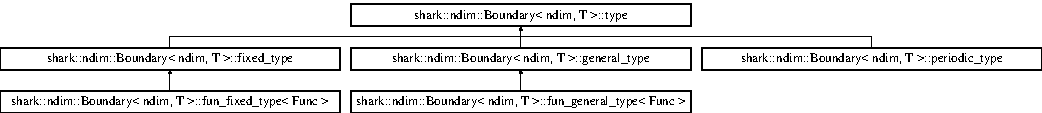
\includegraphics[height=1.521739cm]{classshark_1_1ndim_1_1_boundary_1_1type}
\end{center}
\end{figure}
\subsection*{Public Member Functions}
\begin{DoxyCompactItemize}
\item 
virtual \hyperlink{classshark_1_1ndim_1_1_boundary_1_1type_a55af4628ea73154253616df9809587ad}{$\sim$type} ()
\item 
virtual \hyperlink{classshark_1_1ndim_1_1_boundary_1_1type}{type} $\ast$ \hyperlink{classshark_1_1ndim_1_1_boundary_1_1type_a5651988ce3a6c229009d3fa849e820dc}{clone} () const
\end{DoxyCompactItemize}


\subsection{Detailed Description}
\subsubsection*{template$<$int ndim, typename T$>$\newline
class shark\+::ndim\+::\+Boundary$<$ ndim, T $>$\+::type}



Definition at line 29 of file boundary.\+hpp.



\subsection{Constructor \& Destructor Documentation}
\hypertarget{classshark_1_1ndim_1_1_boundary_1_1type_a55af4628ea73154253616df9809587ad}{}\label{classshark_1_1ndim_1_1_boundary_1_1type_a55af4628ea73154253616df9809587ad} 
\index{shark\+::ndim\+::\+Boundary\+::type@{shark\+::ndim\+::\+Boundary\+::type}!````~type@{$\sim$type}}
\index{````~type@{$\sim$type}!shark\+::ndim\+::\+Boundary\+::type@{shark\+::ndim\+::\+Boundary\+::type}}
\subsubsection{\texorpdfstring{$\sim$type()}{~type()}}
{\footnotesize\ttfamily template$<$int ndim, typename T $>$ \\
Boundary\+::type\+::$\sim$type (\begin{DoxyParamCaption}{ }\end{DoxyParamCaption})\hspace{0.3cm}{\ttfamily [virtual]}}



Definition at line 14 of file boundary.\+cpp.


\begin{DoxyCode}
14 \{ \}
\end{DoxyCode}


\subsection{Member Function Documentation}
\hypertarget{classshark_1_1ndim_1_1_boundary_1_1type_a5651988ce3a6c229009d3fa849e820dc}{}\label{classshark_1_1ndim_1_1_boundary_1_1type_a5651988ce3a6c229009d3fa849e820dc} 
\index{shark\+::ndim\+::\+Boundary\+::type@{shark\+::ndim\+::\+Boundary\+::type}!clone@{clone}}
\index{clone@{clone}!shark\+::ndim\+::\+Boundary\+::type@{shark\+::ndim\+::\+Boundary\+::type}}
\subsubsection{\texorpdfstring{clone()}{clone()}}
{\footnotesize\ttfamily template$<$int ndim, typename T $>$ \\
\hyperlink{classshark_1_1ndim_1_1_boundary}{Boundary}$<$ ndim, T $>$\+::\hyperlink{classshark_1_1ndim_1_1_boundary_1_1type}{type} $\ast$ Boundary\+::type\+::clone (\begin{DoxyParamCaption}{ }\end{DoxyParamCaption}) const\hspace{0.3cm}{\ttfamily [virtual]}}



Reimplemented in \hyperlink{classshark_1_1ndim_1_1_boundary_1_1fun__general__type_a2a2ebd25aa8dcb4960c28db87680e7c6}{shark\+::ndim\+::\+Boundary$<$ ndim, T $>$\+::fun\+\_\+general\+\_\+type$<$ Func $>$}, \hyperlink{classshark_1_1ndim_1_1_boundary_1_1fun__fixed__type_a54ad8e702f2f3ff9403d43bfb7b38411}{shark\+::ndim\+::\+Boundary$<$ ndim, T $>$\+::fun\+\_\+fixed\+\_\+type$<$ Func $>$}, and \hyperlink{classshark_1_1ndim_1_1_boundary_1_1periodic__type_a54904c3d305d26abe8cc8f4b85d9d7e0}{shark\+::ndim\+::\+Boundary$<$ ndim, T $>$\+::periodic\+\_\+type}.



Definition at line 17 of file boundary.\+cpp.


\begin{DoxyCode}
17                                                                  \{
18     \textcolor{keywordflow}{return} \textcolor{keyword}{new} type();
19 \}
\end{DoxyCode}


The documentation for this class was generated from the following files\+:\begin{DoxyCompactItemize}
\item 
include/shark/\hyperlink{boundary_8hpp}{boundary.\+hpp}\item 
src/\hyperlink{boundary_8cpp}{boundary.\+cpp}\end{DoxyCompactItemize}

\hypertarget{classshark_1_1ndim_1_1_unary_acc}{}\section{shark\+:\+:ndim\+:\+:Unary\+Acc$<$ S, Func $>$ Class Template Reference}
\label{classshark_1_1ndim_1_1_unary_acc}\index{shark\+::ndim\+::\+Unary\+Acc$<$ S, Func $>$@{shark\+::ndim\+::\+Unary\+Acc$<$ S, Func $>$}}


{\ttfamily \#include $<$expr.\+hpp$>$}

\subsection*{Public Member Functions}
\begin{DoxyCompactItemize}
\item 
\hyperlink{classshark_1_1ndim_1_1_unary_acc_a776fc8713e13051d4fb52eeef18c067f}{Unary\+Acc} (const \hyperlink{classshark_1_1ndim_1_1_unary_exp}{Unary\+Exp}$<$ S, Func $>$ \&exp)
\item 
\hyperlink{classshark_1_1ndim_1_1_unary_acc_a4069b14973b6098c878dd467d695f7a7}{$\sim$\+Unary\+Acc} ()
\item 
decltype(std\+::declval$<$ Func $>$()(std\+::declval$<$ typename S\+::accessor $>$(), std\+::declval$<$ \hyperlink{structshark_1_1ndim_1_1coords}{coords}$<$ S\+::number\+\_\+of\+\_\+dimensions $>$$>$())) \hyperlink{common_8hpp_a2eb6f9e0395b47b8d5e3eeae4fe0c116}{I\+N\+L\+I\+NE} \hyperlink{classshark_1_1ndim_1_1_unary_acc_ab9a95cebe1e0acf123a375b32743453b}{operator()} (\hyperlink{structshark_1_1ndim_1_1coords}{coords}$<$ S\+::number\+\_\+of\+\_\+dimensions $>$ ii) const
\end{DoxyCompactItemize}
\subsection*{Private Attributes}
\begin{DoxyCompactItemize}
\item 
const S\+::accessor \hyperlink{classshark_1_1ndim_1_1_unary_acc_af254b8e0cfc968269a4e03d80f45a4eb}{a}
\item 
const Func \& \hyperlink{classshark_1_1ndim_1_1_unary_acc_a8a6488ae3b1f64726413bd49721e05b3}{f}
\end{DoxyCompactItemize}


\subsection{Detailed Description}
\subsubsection*{template$<$typename S, typename Func$>$\newline
class shark\+::ndim\+::\+Unary\+Acc$<$ S, Func $>$}

Unary expressions 

Definition at line 126 of file expr.\+hpp.



\subsection{Constructor \& Destructor Documentation}
\hypertarget{classshark_1_1ndim_1_1_unary_acc_a776fc8713e13051d4fb52eeef18c067f}{}\label{classshark_1_1ndim_1_1_unary_acc_a776fc8713e13051d4fb52eeef18c067f} 
\index{shark\+::ndim\+::\+Unary\+Acc@{shark\+::ndim\+::\+Unary\+Acc}!Unary\+Acc@{Unary\+Acc}}
\index{Unary\+Acc@{Unary\+Acc}!shark\+::ndim\+::\+Unary\+Acc@{shark\+::ndim\+::\+Unary\+Acc}}
\subsubsection{\texorpdfstring{Unary\+Acc()}{UnaryAcc()}}
{\footnotesize\ttfamily template$<$typename S , typename Func $>$ \\
\hyperlink{classshark_1_1ndim_1_1_unary_acc}{shark\+::ndim\+::\+Unary\+Acc}$<$ S, Func $>$\+::\hyperlink{classshark_1_1ndim_1_1_unary_acc}{Unary\+Acc} (\begin{DoxyParamCaption}\item[{const \hyperlink{classshark_1_1ndim_1_1_unary_exp}{Unary\+Exp}$<$ S, Func $>$ \&}]{exp }\end{DoxyParamCaption})}



Definition at line 177 of file expr.\+hpp.


\begin{DoxyCode}
177 : \hyperlink{classshark_1_1ndim_1_1_unary_acc_af254b8e0cfc968269a4e03d80f45a4eb}{a}(exp.src), \hyperlink{classshark_1_1ndim_1_1_unary_acc_a8a6488ae3b1f64726413bd49721e05b3}{f}(exp.f) \{ \}
\end{DoxyCode}
\hypertarget{classshark_1_1ndim_1_1_unary_acc_a4069b14973b6098c878dd467d695f7a7}{}\label{classshark_1_1ndim_1_1_unary_acc_a4069b14973b6098c878dd467d695f7a7} 
\index{shark\+::ndim\+::\+Unary\+Acc@{shark\+::ndim\+::\+Unary\+Acc}!````~Unary\+Acc@{$\sim$\+Unary\+Acc}}
\index{````~Unary\+Acc@{$\sim$\+Unary\+Acc}!shark\+::ndim\+::\+Unary\+Acc@{shark\+::ndim\+::\+Unary\+Acc}}
\subsubsection{\texorpdfstring{$\sim$\+Unary\+Acc()}{~UnaryAcc()}}
{\footnotesize\ttfamily template$<$typename S , typename Func $>$ \\
\hyperlink{classshark_1_1ndim_1_1_unary_acc}{shark\+::ndim\+::\+Unary\+Acc}$<$ S, Func $>$\+::$\sim$\hyperlink{classshark_1_1ndim_1_1_unary_acc}{Unary\+Acc} (\begin{DoxyParamCaption}{ }\end{DoxyParamCaption})}



Definition at line 180 of file expr.\+hpp.


\begin{DoxyCode}
180 \{ \}
\end{DoxyCode}


\subsection{Member Function Documentation}
\hypertarget{classshark_1_1ndim_1_1_unary_acc_ab9a95cebe1e0acf123a375b32743453b}{}\label{classshark_1_1ndim_1_1_unary_acc_ab9a95cebe1e0acf123a375b32743453b} 
\index{shark\+::ndim\+::\+Unary\+Acc@{shark\+::ndim\+::\+Unary\+Acc}!operator()@{operator()}}
\index{operator()@{operator()}!shark\+::ndim\+::\+Unary\+Acc@{shark\+::ndim\+::\+Unary\+Acc}}
\subsubsection{\texorpdfstring{operator()()}{operator()()}}
{\footnotesize\ttfamily template$<$typename S , typename Func $>$ \\
decltype(std\+::declval$<$Func$>$()(std\+::declval$<$typename S\+::accessor$>$(), std\+::declval$<$\hyperlink{structshark_1_1ndim_1_1coords}{coords}$<$S\+::number\+\_\+of\+\_\+dimensions$>$$>$())) \hyperlink{common_8hpp_a2eb6f9e0395b47b8d5e3eeae4fe0c116}{I\+N\+L\+I\+NE} \hyperlink{classshark_1_1ndim_1_1_unary_acc}{shark\+::ndim\+::\+Unary\+Acc}$<$ S, Func $>$\+::operator() (\begin{DoxyParamCaption}\item[{\hyperlink{structshark_1_1ndim_1_1coords}{coords}$<$ S\+::number\+\_\+of\+\_\+dimensions $>$}]{ii }\end{DoxyParamCaption}) const}



\subsection{Member Data Documentation}
\hypertarget{classshark_1_1ndim_1_1_unary_acc_af254b8e0cfc968269a4e03d80f45a4eb}{}\label{classshark_1_1ndim_1_1_unary_acc_af254b8e0cfc968269a4e03d80f45a4eb} 
\index{shark\+::ndim\+::\+Unary\+Acc@{shark\+::ndim\+::\+Unary\+Acc}!a@{a}}
\index{a@{a}!shark\+::ndim\+::\+Unary\+Acc@{shark\+::ndim\+::\+Unary\+Acc}}
\subsubsection{\texorpdfstring{a}{a}}
{\footnotesize\ttfamily template$<$typename S , typename Func $>$ \\
const S\+::accessor \hyperlink{classshark_1_1ndim_1_1_unary_acc}{shark\+::ndim\+::\+Unary\+Acc}$<$ S, Func $>$\+::a\hspace{0.3cm}{\ttfamily [private]}}



Definition at line 164 of file expr.\+hpp.

\hypertarget{classshark_1_1ndim_1_1_unary_acc_a8a6488ae3b1f64726413bd49721e05b3}{}\label{classshark_1_1ndim_1_1_unary_acc_a8a6488ae3b1f64726413bd49721e05b3} 
\index{shark\+::ndim\+::\+Unary\+Acc@{shark\+::ndim\+::\+Unary\+Acc}!f@{f}}
\index{f@{f}!shark\+::ndim\+::\+Unary\+Acc@{shark\+::ndim\+::\+Unary\+Acc}}
\subsubsection{\texorpdfstring{f}{f}}
{\footnotesize\ttfamily template$<$typename S , typename Func $>$ \\
const Func\& \hyperlink{classshark_1_1ndim_1_1_unary_acc}{shark\+::ndim\+::\+Unary\+Acc}$<$ S, Func $>$\+::f\hspace{0.3cm}{\ttfamily [private]}}



Definition at line 165 of file expr.\+hpp.



The documentation for this class was generated from the following file\+:\begin{DoxyCompactItemize}
\item 
include/shark/\hyperlink{expr_8hpp}{expr.\+hpp}\end{DoxyCompactItemize}

\hypertarget{classshark_1_1ndim_1_1_unary_exp}{}\section{shark\+:\+:ndim\+:\+:Unary\+Exp$<$ S, Func $>$ Class Template Reference}
\label{classshark_1_1ndim_1_1_unary_exp}\index{shark\+::ndim\+::\+Unary\+Exp$<$ S, Func $>$@{shark\+::ndim\+::\+Unary\+Exp$<$ S, Func $>$}}


{\ttfamily \#include $<$expr.\+hpp$>$}

\subsection*{Public Types}
\begin{DoxyCompactItemize}
\item 
typedef \hyperlink{classshark_1_1ndim_1_1_unary_exp}{Unary\+Exp}$<$ S, Func $>$ \hyperlink{classshark_1_1ndim_1_1_unary_exp_aff41674c204a5df02b79b518efa8ea5b}{storage}
\item 
typedef \hyperlink{classshark_1_1ndim_1_1_unary_acc}{Unary\+Acc}$<$ S, Func $>$ \hyperlink{classshark_1_1ndim_1_1_unary_exp_aa34e1f563bfcee209cd2c1886fe7320f}{accessor}
\end{DoxyCompactItemize}
\subsection*{Public Member Functions}
\begin{DoxyCompactItemize}
\item 
\hyperlink{classshark_1_1ndim_1_1_unary_exp_a5b4b3528aa72c169b82dbd699ddbdf5f}{Unary\+Exp} (const S \&\hyperlink{classshark_1_1ndim_1_1_unary_exp_ad43011a53ffbee999334c7cc52fb95ad}{src}, const Func \&\hyperlink{classshark_1_1ndim_1_1_unary_exp_a7d3fe16a63fc7e035839407f24b586b9}{f})
\item 
\hyperlink{classshark_1_1ndim_1_1_unary_exp_a602b169be3f0bda9f2d668daf01e5ca2}{$\sim$\+Unary\+Exp} ()
\item 
\hyperlink{common_8hpp_a2eb6f9e0395b47b8d5e3eeae4fe0c116}{I\+N\+L\+I\+NE} const \hyperlink{classshark_1_1ndim_1_1_domain}{Domain}$<$ S\+::number\+\_\+of\+\_\+dimensions $>$ \& \hyperlink{classshark_1_1ndim_1_1_unary_exp_a87bc70f88d3c8d535984595b20e4def3}{domain} () const
\item 
\hyperlink{common_8hpp_a2eb6f9e0395b47b8d5e3eeae4fe0c116}{I\+N\+L\+I\+NE} \hyperlink{structshark_1_1ndim_1_1coords__range}{coords\+\_\+range}$<$ S\+::number\+\_\+of\+\_\+dimensions $>$ \hyperlink{classshark_1_1ndim_1_1_unary_exp_ab5cbee53029546b1c0f87f98c4f34616}{region} () const
\end{DoxyCompactItemize}
\subsection*{Static Public Attributes}
\begin{DoxyCompactItemize}
\item 
static const int \hyperlink{classshark_1_1ndim_1_1_unary_exp_a333e05cf6d425d7f42b3f7eb575e6bcb}{number\+\_\+of\+\_\+dimensions} = S\+::number\+\_\+of\+\_\+dimensions
\end{DoxyCompactItemize}
\subsection*{Private Attributes}
\begin{DoxyCompactItemize}
\item 
const S\+::storage \hyperlink{classshark_1_1ndim_1_1_unary_exp_ad43011a53ffbee999334c7cc52fb95ad}{src}
\item 
const Func \hyperlink{classshark_1_1ndim_1_1_unary_exp_a7d3fe16a63fc7e035839407f24b586b9}{f}
\end{DoxyCompactItemize}
\subsection*{Friends}
\begin{DoxyCompactItemize}
\item 
class \hyperlink{classshark_1_1ndim_1_1_unary_exp_a022f283e42a9d39735bdcf5d954349f1}{Unary\+Acc$<$ S, Func $>$}
\end{DoxyCompactItemize}


\subsection{Detailed Description}
\subsubsection*{template$<$typename S, typename Func$>$\newline
class shark\+::ndim\+::\+Unary\+Exp$<$ S, Func $>$}



Definition at line 129 of file expr.\+hpp.



\subsection{Member Typedef Documentation}
\hypertarget{classshark_1_1ndim_1_1_unary_exp_aa34e1f563bfcee209cd2c1886fe7320f}{}\label{classshark_1_1ndim_1_1_unary_exp_aa34e1f563bfcee209cd2c1886fe7320f} 
\index{shark\+::ndim\+::\+Unary\+Exp@{shark\+::ndim\+::\+Unary\+Exp}!accessor@{accessor}}
\index{accessor@{accessor}!shark\+::ndim\+::\+Unary\+Exp@{shark\+::ndim\+::\+Unary\+Exp}}
\subsubsection{\texorpdfstring{accessor}{accessor}}
{\footnotesize\ttfamily template$<$typename S, typename Func$>$ \\
typedef \hyperlink{classshark_1_1ndim_1_1_unary_acc}{Unary\+Acc}$<$S,Func$>$ \hyperlink{classshark_1_1ndim_1_1_unary_exp}{shark\+::ndim\+::\+Unary\+Exp}$<$ S, Func $>$\+::\hyperlink{classshark_1_1ndim_1_1_unary_exp_aa34e1f563bfcee209cd2c1886fe7320f}{accessor}}



Definition at line 136 of file expr.\+hpp.

\hypertarget{classshark_1_1ndim_1_1_unary_exp_aff41674c204a5df02b79b518efa8ea5b}{}\label{classshark_1_1ndim_1_1_unary_exp_aff41674c204a5df02b79b518efa8ea5b} 
\index{shark\+::ndim\+::\+Unary\+Exp@{shark\+::ndim\+::\+Unary\+Exp}!storage@{storage}}
\index{storage@{storage}!shark\+::ndim\+::\+Unary\+Exp@{shark\+::ndim\+::\+Unary\+Exp}}
\subsubsection{\texorpdfstring{storage}{storage}}
{\footnotesize\ttfamily template$<$typename S, typename Func$>$ \\
typedef \hyperlink{classshark_1_1ndim_1_1_unary_exp}{Unary\+Exp}$<$S,Func$>$ \hyperlink{classshark_1_1ndim_1_1_unary_exp}{shark\+::ndim\+::\+Unary\+Exp}$<$ S, Func $>$\+::\hyperlink{classshark_1_1ndim_1_1_unary_exp_aff41674c204a5df02b79b518efa8ea5b}{storage}}



Definition at line 135 of file expr.\+hpp.



\subsection{Constructor \& Destructor Documentation}
\hypertarget{classshark_1_1ndim_1_1_unary_exp_a5b4b3528aa72c169b82dbd699ddbdf5f}{}\label{classshark_1_1ndim_1_1_unary_exp_a5b4b3528aa72c169b82dbd699ddbdf5f} 
\index{shark\+::ndim\+::\+Unary\+Exp@{shark\+::ndim\+::\+Unary\+Exp}!Unary\+Exp@{Unary\+Exp}}
\index{Unary\+Exp@{Unary\+Exp}!shark\+::ndim\+::\+Unary\+Exp@{shark\+::ndim\+::\+Unary\+Exp}}
\subsubsection{\texorpdfstring{Unary\+Exp()}{UnaryExp()}}
{\footnotesize\ttfamily template$<$typename S , typename Func $>$ \\
\hyperlink{classshark_1_1ndim_1_1_unary_exp}{shark\+::ndim\+::\+Unary\+Exp}$<$ S, Func $>$\+::\hyperlink{classshark_1_1ndim_1_1_unary_exp}{Unary\+Exp} (\begin{DoxyParamCaption}\item[{const S \&}]{src,  }\item[{const Func \&}]{f }\end{DoxyParamCaption})}



Definition at line 147 of file expr.\+hpp.


\begin{DoxyCode}
147 : \hyperlink{classshark_1_1ndim_1_1_unary_exp_ad43011a53ffbee999334c7cc52fb95ad}{src}(\hyperlink{classshark_1_1ndim_1_1_unary_exp_ad43011a53ffbee999334c7cc52fb95ad}{src}), \hyperlink{classshark_1_1ndim_1_1_unary_exp_a7d3fe16a63fc7e035839407f24b586b9}{f}(\hyperlink{classshark_1_1ndim_1_1_unary_exp_a7d3fe16a63fc7e035839407f24b586b9}{f}) \{ \}
\end{DoxyCode}
\hypertarget{classshark_1_1ndim_1_1_unary_exp_a602b169be3f0bda9f2d668daf01e5ca2}{}\label{classshark_1_1ndim_1_1_unary_exp_a602b169be3f0bda9f2d668daf01e5ca2} 
\index{shark\+::ndim\+::\+Unary\+Exp@{shark\+::ndim\+::\+Unary\+Exp}!````~Unary\+Exp@{$\sim$\+Unary\+Exp}}
\index{````~Unary\+Exp@{$\sim$\+Unary\+Exp}!shark\+::ndim\+::\+Unary\+Exp@{shark\+::ndim\+::\+Unary\+Exp}}
\subsubsection{\texorpdfstring{$\sim$\+Unary\+Exp()}{~UnaryExp()}}
{\footnotesize\ttfamily template$<$typename S , typename Func $>$ \\
\hyperlink{classshark_1_1ndim_1_1_unary_exp}{shark\+::ndim\+::\+Unary\+Exp}$<$ S, Func $>$\+::$\sim$\hyperlink{classshark_1_1ndim_1_1_unary_exp}{Unary\+Exp} (\begin{DoxyParamCaption}{ }\end{DoxyParamCaption})}



Definition at line 150 of file expr.\+hpp.


\begin{DoxyCode}
150 \{ \}
\end{DoxyCode}


\subsection{Member Function Documentation}
\hypertarget{classshark_1_1ndim_1_1_unary_exp_a87bc70f88d3c8d535984595b20e4def3}{}\label{classshark_1_1ndim_1_1_unary_exp_a87bc70f88d3c8d535984595b20e4def3} 
\index{shark\+::ndim\+::\+Unary\+Exp@{shark\+::ndim\+::\+Unary\+Exp}!domain@{domain}}
\index{domain@{domain}!shark\+::ndim\+::\+Unary\+Exp@{shark\+::ndim\+::\+Unary\+Exp}}
\subsubsection{\texorpdfstring{domain()}{domain()}}
{\footnotesize\ttfamily template$<$typename S , typename Func $>$ \\
const \hyperlink{classshark_1_1ndim_1_1_domain}{Domain}$<$ S\+::number\+\_\+of\+\_\+dimensions $>$ \& \hyperlink{classshark_1_1ndim_1_1_unary_exp}{shark\+::ndim\+::\+Unary\+Exp}$<$ S, Func $>$\+::domain (\begin{DoxyParamCaption}{ }\end{DoxyParamCaption}) const\hspace{0.3cm}{\ttfamily [inline]}}



Definition at line 153 of file expr.\+hpp.


\begin{DoxyCode}
153                                                                                    \{
154             \textcolor{keywordflow}{return} \hyperlink{classshark_1_1ndim_1_1_unary_exp_ad43011a53ffbee999334c7cc52fb95ad}{src}.domain();
155         \}
\end{DoxyCode}
\hypertarget{classshark_1_1ndim_1_1_unary_exp_ab5cbee53029546b1c0f87f98c4f34616}{}\label{classshark_1_1ndim_1_1_unary_exp_ab5cbee53029546b1c0f87f98c4f34616} 
\index{shark\+::ndim\+::\+Unary\+Exp@{shark\+::ndim\+::\+Unary\+Exp}!region@{region}}
\index{region@{region}!shark\+::ndim\+::\+Unary\+Exp@{shark\+::ndim\+::\+Unary\+Exp}}
\subsubsection{\texorpdfstring{region()}{region()}}
{\footnotesize\ttfamily template$<$typename S , typename Func $>$ \\
\hyperlink{structshark_1_1ndim_1_1coords__range}{coords\+\_\+range}$<$ S\+::number\+\_\+of\+\_\+dimensions $>$ \hyperlink{classshark_1_1ndim_1_1_unary_exp}{shark\+::ndim\+::\+Unary\+Exp}$<$ S, Func $>$\+::region (\begin{DoxyParamCaption}{ }\end{DoxyParamCaption}) const\hspace{0.3cm}{\ttfamily [inline]}}



Definition at line 158 of file expr.\+hpp.


\begin{DoxyCode}
158                                                                                   \{
159             \textcolor{keywordflow}{return} \hyperlink{classshark_1_1ndim_1_1_unary_exp_ad43011a53ffbee999334c7cc52fb95ad}{src}.region();
160         \}
\end{DoxyCode}


\subsection{Friends And Related Function Documentation}
\hypertarget{classshark_1_1ndim_1_1_unary_exp_a022f283e42a9d39735bdcf5d954349f1}{}\label{classshark_1_1ndim_1_1_unary_exp_a022f283e42a9d39735bdcf5d954349f1} 
\index{shark\+::ndim\+::\+Unary\+Exp@{shark\+::ndim\+::\+Unary\+Exp}!Unary\+Acc$<$ S, Func $>$@{Unary\+Acc$<$ S, Func $>$}}
\index{Unary\+Acc$<$ S, Func $>$@{Unary\+Acc$<$ S, Func $>$}!shark\+::ndim\+::\+Unary\+Exp@{shark\+::ndim\+::\+Unary\+Exp}}
\subsubsection{\texorpdfstring{Unary\+Acc$<$ S, Func $>$}{UnaryAcc< S, Func >}}
{\footnotesize\ttfamily template$<$typename S, typename Func$>$ \\
friend class \hyperlink{classshark_1_1ndim_1_1_unary_acc}{Unary\+Acc}$<$ S, Func $>$\hspace{0.3cm}{\ttfamily [friend]}}



Definition at line 130 of file expr.\+hpp.



\subsection{Member Data Documentation}
\hypertarget{classshark_1_1ndim_1_1_unary_exp_a7d3fe16a63fc7e035839407f24b586b9}{}\label{classshark_1_1ndim_1_1_unary_exp_a7d3fe16a63fc7e035839407f24b586b9} 
\index{shark\+::ndim\+::\+Unary\+Exp@{shark\+::ndim\+::\+Unary\+Exp}!f@{f}}
\index{f@{f}!shark\+::ndim\+::\+Unary\+Exp@{shark\+::ndim\+::\+Unary\+Exp}}
\subsubsection{\texorpdfstring{f}{f}}
{\footnotesize\ttfamily template$<$typename S, typename Func$>$ \\
const Func \hyperlink{classshark_1_1ndim_1_1_unary_exp}{shark\+::ndim\+::\+Unary\+Exp}$<$ S, Func $>$\+::f\hspace{0.3cm}{\ttfamily [private]}}



Definition at line 132 of file expr.\+hpp.

\hypertarget{classshark_1_1ndim_1_1_unary_exp_a333e05cf6d425d7f42b3f7eb575e6bcb}{}\label{classshark_1_1ndim_1_1_unary_exp_a333e05cf6d425d7f42b3f7eb575e6bcb} 
\index{shark\+::ndim\+::\+Unary\+Exp@{shark\+::ndim\+::\+Unary\+Exp}!number\+\_\+of\+\_\+dimensions@{number\+\_\+of\+\_\+dimensions}}
\index{number\+\_\+of\+\_\+dimensions@{number\+\_\+of\+\_\+dimensions}!shark\+::ndim\+::\+Unary\+Exp@{shark\+::ndim\+::\+Unary\+Exp}}
\subsubsection{\texorpdfstring{number\+\_\+of\+\_\+dimensions}{number\_of\_dimensions}}
{\footnotesize\ttfamily template$<$typename S, typename Func$>$ \\
const int \hyperlink{classshark_1_1ndim_1_1_unary_exp}{shark\+::ndim\+::\+Unary\+Exp}$<$ S, Func $>$\+::number\+\_\+of\+\_\+dimensions = S\+::number\+\_\+of\+\_\+dimensions\hspace{0.3cm}{\ttfamily [static]}}



Definition at line 134 of file expr.\+hpp.

\hypertarget{classshark_1_1ndim_1_1_unary_exp_ad43011a53ffbee999334c7cc52fb95ad}{}\label{classshark_1_1ndim_1_1_unary_exp_ad43011a53ffbee999334c7cc52fb95ad} 
\index{shark\+::ndim\+::\+Unary\+Exp@{shark\+::ndim\+::\+Unary\+Exp}!src@{src}}
\index{src@{src}!shark\+::ndim\+::\+Unary\+Exp@{shark\+::ndim\+::\+Unary\+Exp}}
\subsubsection{\texorpdfstring{src}{src}}
{\footnotesize\ttfamily template$<$typename S, typename Func$>$ \\
const S\+::storage \hyperlink{classshark_1_1ndim_1_1_unary_exp}{shark\+::ndim\+::\+Unary\+Exp}$<$ S, Func $>$\+::src\hspace{0.3cm}{\ttfamily [private]}}



Definition at line 131 of file expr.\+hpp.



The documentation for this class was generated from the following file\+:\begin{DoxyCompactItemize}
\item 
include/shark/\hyperlink{expr_8hpp}{expr.\+hpp}\end{DoxyCompactItemize}

\hypertarget{structshark_1_1ndim_1_1vec}{}\section{shark\+:\+:ndim\+:\+:vec$<$ ndim, T $>$ Struct Template Reference}
\label{structshark_1_1ndim_1_1vec}\index{shark\+::ndim\+::vec$<$ ndim, T $>$@{shark\+::ndim\+::vec$<$ ndim, T $>$}}


{\ttfamily \#include $<$vec.\+hpp$>$}

\subsection*{Public Member Functions}
\begin{DoxyCompactItemize}
\item 
\hyperlink{common_8hpp_a2eb6f9e0395b47b8d5e3eeae4fe0c116}{I\+N\+L\+I\+NE} T \& \hyperlink{structshark_1_1ndim_1_1vec_ab5506a5f5d9f1f8a2722626620fa305c}{operator\mbox{[}$\,$\mbox{]}} (int d)
\item 
\hyperlink{common_8hpp_a2eb6f9e0395b47b8d5e3eeae4fe0c116}{I\+N\+L\+I\+NE} const T \& \hyperlink{structshark_1_1ndim_1_1vec_a7ef60f43a2b6e0429a85ab67f323bd59}{operator\mbox{[}$\,$\mbox{]}} (int d) const
\item 
\hyperlink{common_8hpp_a2eb6f9e0395b47b8d5e3eeae4fe0c116}{I\+N\+L\+I\+NE} bool \hyperlink{structshark_1_1ndim_1_1vec_a796dd27a2b072a4b5e0618bb5851bfa8}{operator==} (const \hyperlink{structshark_1_1ndim_1_1vec}{vec}$<$ ndim, T $>$ \&other) const
\item 
\hyperlink{common_8hpp_a2eb6f9e0395b47b8d5e3eeae4fe0c116}{I\+N\+L\+I\+NE} bool \hyperlink{structshark_1_1ndim_1_1vec_af57ada01823047ae447cc294e4c4bfe0}{operator!=} (const \hyperlink{structshark_1_1ndim_1_1vec}{vec}$<$ ndim, T $>$ \&other) const
\item 
{\footnotesize template$<$typename S $>$ }\\\hyperlink{common_8hpp_a2eb6f9e0395b47b8d5e3eeae4fe0c116}{I\+N\+L\+I\+NE} \hyperlink{structshark_1_1ndim_1_1vec}{vec}$<$ ndim, T $>$ \& \hyperlink{structshark_1_1ndim_1_1vec_a126750e81729ae1c0ccfb60e1eff5ed0}{operator+=} (const \hyperlink{structshark_1_1ndim_1_1vec}{vec}$<$ ndim, S $>$ \&other)
\item 
{\footnotesize template$<$typename S $>$ }\\\hyperlink{common_8hpp_a2eb6f9e0395b47b8d5e3eeae4fe0c116}{I\+N\+L\+I\+NE} \hyperlink{structshark_1_1ndim_1_1vec}{vec}$<$ ndim, T $>$ \& \hyperlink{structshark_1_1ndim_1_1vec_a1fd95421a7d7d555f9e7861f807f79ab}{operator-\/=} (const \hyperlink{structshark_1_1ndim_1_1vec}{vec}$<$ ndim, S $>$ \&other)
\item 
{\footnotesize template$<$typename S $>$ }\\\hyperlink{common_8hpp_a2eb6f9e0395b47b8d5e3eeae4fe0c116}{I\+N\+L\+I\+NE} \hyperlink{structshark_1_1ndim_1_1vec}{vec}$<$ ndim, T $>$ \& \hyperlink{structshark_1_1ndim_1_1vec_a3b6b703d38be32f4d543718743026582}{operator$\ast$=} (const \hyperlink{structshark_1_1ndim_1_1vec}{vec}$<$ ndim, S $>$ \&other)
\item 
{\footnotesize template$<$typename S $>$ }\\\hyperlink{common_8hpp_a2eb6f9e0395b47b8d5e3eeae4fe0c116}{I\+N\+L\+I\+NE} \hyperlink{structshark_1_1ndim_1_1vec}{vec}$<$ ndim, T $>$ \& \hyperlink{structshark_1_1ndim_1_1vec_a640e4ea895ad8b14a259249227bc9290}{operator/=} (const \hyperlink{structshark_1_1ndim_1_1vec}{vec}$<$ ndim, S $>$ \&other)
\item 
\hyperlink{common_8hpp_a2eb6f9e0395b47b8d5e3eeae4fe0c116}{I\+N\+L\+I\+NE} T \hyperlink{structshark_1_1ndim_1_1vec_a8db2f3a20f6cbf6cc2ebf9ecb00e0cc4}{min} () const
\item 
\hyperlink{common_8hpp_a2eb6f9e0395b47b8d5e3eeae4fe0c116}{I\+N\+L\+I\+NE} T \hyperlink{structshark_1_1ndim_1_1vec_aabdbb224acc832abb50f9a0ab739533a}{max} () const
\item 
{\footnotesize template$<$typename S $>$ }\\\hyperlink{structshark_1_1ndim_1_1vec}{vec}$<$ ndim, T $>$ \& \hyperlink{structshark_1_1ndim_1_1vec_af89f86b8ee43b2c1a0adb9bd8223d548}{operator+=} (const \hyperlink{structshark_1_1ndim_1_1vec}{vec}$<$ ndim, S $>$ \&other)
\item 
{\footnotesize template$<$typename S $>$ }\\\hyperlink{structshark_1_1ndim_1_1vec}{vec}$<$ ndim, T $>$ \& \hyperlink{structshark_1_1ndim_1_1vec_accad5ec69cc6833eae34802f1a7c81ac}{operator-\/=} (const \hyperlink{structshark_1_1ndim_1_1vec}{vec}$<$ ndim, S $>$ \&other)
\item 
{\footnotesize template$<$typename S $>$ }\\\hyperlink{structshark_1_1ndim_1_1vec}{vec}$<$ ndim, T $>$ \& \hyperlink{structshark_1_1ndim_1_1vec_af52bce704e4bd632c3844614007ca5ce}{operator$\ast$=} (const \hyperlink{structshark_1_1ndim_1_1vec}{vec}$<$ ndim, S $>$ \&other)
\item 
{\footnotesize template$<$typename S $>$ }\\\hyperlink{structshark_1_1ndim_1_1vec}{vec}$<$ ndim, T $>$ \& \hyperlink{structshark_1_1ndim_1_1vec_a9b9aa95a9329ad2877f57c62774063e1}{operator/=} (const \hyperlink{structshark_1_1ndim_1_1vec}{vec}$<$ ndim, S $>$ \&other)
\end{DoxyCompactItemize}
\subsection*{Static Public Member Functions}
\begin{DoxyCompactItemize}
\item 
static \hyperlink{common_8hpp_a2eb6f9e0395b47b8d5e3eeae4fe0c116}{I\+N\+L\+I\+NE} \hyperlink{structshark_1_1ndim_1_1vec}{vec}$<$ ndim, T $>$ \hyperlink{structshark_1_1ndim_1_1vec_a96c9d1e9b072fbe2cb8ac4f229e25e85}{one} ()
\end{DoxyCompactItemize}
\subsection*{Public Attributes}
\begin{DoxyCompactItemize}
\item 
T \hyperlink{structshark_1_1ndim_1_1vec_a1769eccc65b4b95dced51726c271d077}{val} \mbox{[}ndim\mbox{]}
\end{DoxyCompactItemize}


\subsection{Detailed Description}
\subsubsection*{template$<$int ndim, typename T$>$\newline
struct shark\+::ndim\+::vec$<$ ndim, T $>$}



Definition at line 19 of file vec.\+hpp.



\subsection{Member Function Documentation}
\hypertarget{structshark_1_1ndim_1_1vec_aabdbb224acc832abb50f9a0ab739533a}{}\label{structshark_1_1ndim_1_1vec_aabdbb224acc832abb50f9a0ab739533a} 
\index{shark\+::ndim\+::vec@{shark\+::ndim\+::vec}!max@{max}}
\index{max@{max}!shark\+::ndim\+::vec@{shark\+::ndim\+::vec}}
\subsubsection{\texorpdfstring{max()}{max()}}
{\footnotesize\ttfamily template$<$int ndim, typename T $>$ \\
T \hyperlink{structshark_1_1ndim_1_1vec}{shark\+::ndim\+::vec}$<$ ndim, T $>$\+::max (\begin{DoxyParamCaption}{ }\end{DoxyParamCaption}) const\hspace{0.3cm}{\ttfamily [inline]}}



Definition at line 128 of file vec.\+hpp.


\begin{DoxyCode}
128                                         \{
129             T cand((*\textcolor{keyword}{this})[0]);
130             seq<1,ndim-1>::for\_each([\textcolor{keyword}{this},&cand](\textcolor{keywordtype}{int} d) \{
131                 \textcolor{keywordflow}{if}((*\textcolor{keyword}{this})[d] > cand)
132                     cand = (*\textcolor{keyword}{this})[d];
133             \});
134             \textcolor{keywordflow}{return} cand;
135         \}
\end{DoxyCode}
\hypertarget{structshark_1_1ndim_1_1vec_a8db2f3a20f6cbf6cc2ebf9ecb00e0cc4}{}\label{structshark_1_1ndim_1_1vec_a8db2f3a20f6cbf6cc2ebf9ecb00e0cc4} 
\index{shark\+::ndim\+::vec@{shark\+::ndim\+::vec}!min@{min}}
\index{min@{min}!shark\+::ndim\+::vec@{shark\+::ndim\+::vec}}
\subsubsection{\texorpdfstring{min()}{min()}}
{\footnotesize\ttfamily template$<$int ndim, typename T $>$ \\
T \hyperlink{structshark_1_1ndim_1_1vec}{shark\+::ndim\+::vec}$<$ ndim, T $>$\+::min (\begin{DoxyParamCaption}{ }\end{DoxyParamCaption}) const\hspace{0.3cm}{\ttfamily [inline]}}



Definition at line 118 of file vec.\+hpp.


\begin{DoxyCode}
118                                         \{
119             T cand((*\textcolor{keyword}{this})[0]);
120             seq<1,ndim-1>::for\_each([\textcolor{keyword}{this},&cand](\textcolor{keywordtype}{int} d) \{
121                 \textcolor{keywordflow}{if}((*\textcolor{keyword}{this})[d] < cand)
122                     cand = (*\textcolor{keyword}{this})[d];
123             \});
124             \textcolor{keywordflow}{return} cand;
125         \}
\end{DoxyCode}
\hypertarget{structshark_1_1ndim_1_1vec_a96c9d1e9b072fbe2cb8ac4f229e25e85}{}\label{structshark_1_1ndim_1_1vec_a96c9d1e9b072fbe2cb8ac4f229e25e85} 
\index{shark\+::ndim\+::vec@{shark\+::ndim\+::vec}!one@{one}}
\index{one@{one}!shark\+::ndim\+::vec@{shark\+::ndim\+::vec}}
\subsubsection{\texorpdfstring{one()}{one()}}
{\footnotesize\ttfamily template$<$int ndim, typename T $>$ \\
\hyperlink{structshark_1_1ndim_1_1vec}{vec}$<$ ndim, T $>$ \hyperlink{structshark_1_1ndim_1_1vec}{shark\+::ndim\+::vec}$<$ ndim, T $>$\+::one (\begin{DoxyParamCaption}{ }\end{DoxyParamCaption})\hspace{0.3cm}{\ttfamily [inline]}, {\ttfamily [static]}}



Definition at line 138 of file vec.\+hpp.


\begin{DoxyCode}
138                                             \{
139             vec<ndim,T> r;
140             seq<0,ndim>::for\_each([&r](\textcolor{keywordtype}{int} d) \{ r[d] = T(1); \});
141             \textcolor{keywordflow}{return} r;
142         \}
\end{DoxyCode}
\hypertarget{structshark_1_1ndim_1_1vec_af57ada01823047ae447cc294e4c4bfe0}{}\label{structshark_1_1ndim_1_1vec_af57ada01823047ae447cc294e4c4bfe0} 
\index{shark\+::ndim\+::vec@{shark\+::ndim\+::vec}!operator"!=@{operator"!=}}
\index{operator"!=@{operator"!=}!shark\+::ndim\+::vec@{shark\+::ndim\+::vec}}
\subsubsection{\texorpdfstring{operator"!=()}{operator!=()}}
{\footnotesize\ttfamily template$<$int ndim, typename T$>$ \\
bool \hyperlink{structshark_1_1ndim_1_1vec}{shark\+::ndim\+::vec}$<$ ndim, T $>$\+::operator!= (\begin{DoxyParamCaption}\item[{const \hyperlink{structshark_1_1ndim_1_1vec}{vec}$<$ ndim, T $>$ \&}]{other }\end{DoxyParamCaption}) const\hspace{0.3cm}{\ttfamily [inline]}}



Definition at line 91 of file vec.\+hpp.


\begin{DoxyCode}
91                                                                           \{
92             \textcolor{keywordflow}{return} !(*\textcolor{keyword}{this} == other);
93         \}
\end{DoxyCode}
\hypertarget{structshark_1_1ndim_1_1vec_a3b6b703d38be32f4d543718743026582}{}\label{structshark_1_1ndim_1_1vec_a3b6b703d38be32f4d543718743026582} 
\index{shark\+::ndim\+::vec@{shark\+::ndim\+::vec}!operator$\ast$=@{operator$\ast$=}}
\index{operator$\ast$=@{operator$\ast$=}!shark\+::ndim\+::vec@{shark\+::ndim\+::vec}}
\subsubsection{\texorpdfstring{operator$\ast$=()}{operator*=()}\hspace{0.1cm}{\footnotesize\ttfamily [1/2]}}
{\footnotesize\ttfamily template$<$int ndim, typename T$>$ \\
template$<$typename S $>$ \\
\hyperlink{common_8hpp_a2eb6f9e0395b47b8d5e3eeae4fe0c116}{I\+N\+L\+I\+NE} \hyperlink{structshark_1_1ndim_1_1vec}{vec}$<$ndim,T$>$\& \hyperlink{structshark_1_1ndim_1_1vec}{shark\+::ndim\+::vec}$<$ ndim, T $>$\+::operator$\ast$= (\begin{DoxyParamCaption}\item[{const \hyperlink{structshark_1_1ndim_1_1vec}{vec}$<$ ndim, S $>$ \&}]{other }\end{DoxyParamCaption})}

\hypertarget{structshark_1_1ndim_1_1vec_af52bce704e4bd632c3844614007ca5ce}{}\label{structshark_1_1ndim_1_1vec_af52bce704e4bd632c3844614007ca5ce} 
\index{shark\+::ndim\+::vec@{shark\+::ndim\+::vec}!operator$\ast$=@{operator$\ast$=}}
\index{operator$\ast$=@{operator$\ast$=}!shark\+::ndim\+::vec@{shark\+::ndim\+::vec}}
\subsubsection{\texorpdfstring{operator$\ast$=()}{operator*=()}\hspace{0.1cm}{\footnotesize\ttfamily [2/2]}}
{\footnotesize\ttfamily template$<$int ndim, typename T$>$ \\
template$<$typename S $>$ \\
\hyperlink{structshark_1_1ndim_1_1vec}{vec}$<$ndim,T$>$\& \hyperlink{structshark_1_1ndim_1_1vec}{shark\+::ndim\+::vec}$<$ ndim, T $>$\+::operator$\ast$= (\begin{DoxyParamCaption}\item[{const \hyperlink{structshark_1_1ndim_1_1vec}{vec}$<$ ndim, S $>$ \&}]{other }\end{DoxyParamCaption})\hspace{0.3cm}{\ttfamily [inline]}}



Definition at line 107 of file vec.\+hpp.


\begin{DoxyCode}
107                                                                             \{
108             seq<0,ndim>::for\_each([\textcolor{keyword}{this},&other](\textcolor{keywordtype}{int} d) \{ (*this)[d] *= other[d]; \});
109             \textcolor{keywordflow}{return} *\textcolor{keyword}{this};
110         \}
\end{DoxyCode}
\hypertarget{structshark_1_1ndim_1_1vec_a126750e81729ae1c0ccfb60e1eff5ed0}{}\label{structshark_1_1ndim_1_1vec_a126750e81729ae1c0ccfb60e1eff5ed0} 
\index{shark\+::ndim\+::vec@{shark\+::ndim\+::vec}!operator+=@{operator+=}}
\index{operator+=@{operator+=}!shark\+::ndim\+::vec@{shark\+::ndim\+::vec}}
\subsubsection{\texorpdfstring{operator+=()}{operator+=()}\hspace{0.1cm}{\footnotesize\ttfamily [1/2]}}
{\footnotesize\ttfamily template$<$int ndim, typename T$>$ \\
template$<$typename S $>$ \\
\hyperlink{common_8hpp_a2eb6f9e0395b47b8d5e3eeae4fe0c116}{I\+N\+L\+I\+NE} \hyperlink{structshark_1_1ndim_1_1vec}{vec}$<$ndim,T$>$\& \hyperlink{structshark_1_1ndim_1_1vec}{shark\+::ndim\+::vec}$<$ ndim, T $>$\+::operator+= (\begin{DoxyParamCaption}\item[{const \hyperlink{structshark_1_1ndim_1_1vec}{vec}$<$ ndim, S $>$ \&}]{other }\end{DoxyParamCaption})}

\hypertarget{structshark_1_1ndim_1_1vec_af89f86b8ee43b2c1a0adb9bd8223d548}{}\label{structshark_1_1ndim_1_1vec_af89f86b8ee43b2c1a0adb9bd8223d548} 
\index{shark\+::ndim\+::vec@{shark\+::ndim\+::vec}!operator+=@{operator+=}}
\index{operator+=@{operator+=}!shark\+::ndim\+::vec@{shark\+::ndim\+::vec}}
\subsubsection{\texorpdfstring{operator+=()}{operator+=()}\hspace{0.1cm}{\footnotesize\ttfamily [2/2]}}
{\footnotesize\ttfamily template$<$int ndim, typename T$>$ \\
template$<$typename S $>$ \\
\hyperlink{structshark_1_1ndim_1_1vec}{vec}$<$ndim,T$>$\& \hyperlink{structshark_1_1ndim_1_1vec}{shark\+::ndim\+::vec}$<$ ndim, T $>$\+::operator+= (\begin{DoxyParamCaption}\item[{const \hyperlink{structshark_1_1ndim_1_1vec}{vec}$<$ ndim, S $>$ \&}]{other }\end{DoxyParamCaption})\hspace{0.3cm}{\ttfamily [inline]}}



Definition at line 96 of file vec.\+hpp.


\begin{DoxyCode}
96                                                                             \{
97             seq<0,ndim>::for\_each([\textcolor{keyword}{this},&other](\textcolor{keywordtype}{int} d) \{ (*this)[d] += other[d]; \});
98             \textcolor{keywordflow}{return} *\textcolor{keyword}{this};
99         \}
\end{DoxyCode}
\hypertarget{structshark_1_1ndim_1_1vec_a1fd95421a7d7d555f9e7861f807f79ab}{}\label{structshark_1_1ndim_1_1vec_a1fd95421a7d7d555f9e7861f807f79ab} 
\index{shark\+::ndim\+::vec@{shark\+::ndim\+::vec}!operator-\/=@{operator-\/=}}
\index{operator-\/=@{operator-\/=}!shark\+::ndim\+::vec@{shark\+::ndim\+::vec}}
\subsubsection{\texorpdfstring{operator-\/=()}{operator-=()}\hspace{0.1cm}{\footnotesize\ttfamily [1/2]}}
{\footnotesize\ttfamily template$<$int ndim, typename T$>$ \\
template$<$typename S $>$ \\
\hyperlink{common_8hpp_a2eb6f9e0395b47b8d5e3eeae4fe0c116}{I\+N\+L\+I\+NE} \hyperlink{structshark_1_1ndim_1_1vec}{vec}$<$ndim,T$>$\& \hyperlink{structshark_1_1ndim_1_1vec}{shark\+::ndim\+::vec}$<$ ndim, T $>$\+::operator-\/= (\begin{DoxyParamCaption}\item[{const \hyperlink{structshark_1_1ndim_1_1vec}{vec}$<$ ndim, S $>$ \&}]{other }\end{DoxyParamCaption})}

\hypertarget{structshark_1_1ndim_1_1vec_accad5ec69cc6833eae34802f1a7c81ac}{}\label{structshark_1_1ndim_1_1vec_accad5ec69cc6833eae34802f1a7c81ac} 
\index{shark\+::ndim\+::vec@{shark\+::ndim\+::vec}!operator-\/=@{operator-\/=}}
\index{operator-\/=@{operator-\/=}!shark\+::ndim\+::vec@{shark\+::ndim\+::vec}}
\subsubsection{\texorpdfstring{operator-\/=()}{operator-=()}\hspace{0.1cm}{\footnotesize\ttfamily [2/2]}}
{\footnotesize\ttfamily template$<$int ndim, typename T$>$ \\
template$<$typename S $>$ \\
\hyperlink{structshark_1_1ndim_1_1vec}{vec}$<$ndim,T$>$\& \hyperlink{structshark_1_1ndim_1_1vec}{shark\+::ndim\+::vec}$<$ ndim, T $>$\+::operator-\/= (\begin{DoxyParamCaption}\item[{const \hyperlink{structshark_1_1ndim_1_1vec}{vec}$<$ ndim, S $>$ \&}]{other }\end{DoxyParamCaption})\hspace{0.3cm}{\ttfamily [inline]}}



Definition at line 102 of file vec.\+hpp.


\begin{DoxyCode}
102                                                                             \{
103             seq<0,ndim>::for\_each([\textcolor{keyword}{this},&other](\textcolor{keywordtype}{int} d) \{ (*this)[d] -= other[d]; \});
104             \textcolor{keywordflow}{return} *\textcolor{keyword}{this};
105         \}
\end{DoxyCode}
\hypertarget{structshark_1_1ndim_1_1vec_a640e4ea895ad8b14a259249227bc9290}{}\label{structshark_1_1ndim_1_1vec_a640e4ea895ad8b14a259249227bc9290} 
\index{shark\+::ndim\+::vec@{shark\+::ndim\+::vec}!operator/=@{operator/=}}
\index{operator/=@{operator/=}!shark\+::ndim\+::vec@{shark\+::ndim\+::vec}}
\subsubsection{\texorpdfstring{operator/=()}{operator/=()}\hspace{0.1cm}{\footnotesize\ttfamily [1/2]}}
{\footnotesize\ttfamily template$<$int ndim, typename T$>$ \\
template$<$typename S $>$ \\
\hyperlink{common_8hpp_a2eb6f9e0395b47b8d5e3eeae4fe0c116}{I\+N\+L\+I\+NE} \hyperlink{structshark_1_1ndim_1_1vec}{vec}$<$ndim,T$>$\& \hyperlink{structshark_1_1ndim_1_1vec}{shark\+::ndim\+::vec}$<$ ndim, T $>$\+::operator/= (\begin{DoxyParamCaption}\item[{const \hyperlink{structshark_1_1ndim_1_1vec}{vec}$<$ ndim, S $>$ \&}]{other }\end{DoxyParamCaption})}

\hypertarget{structshark_1_1ndim_1_1vec_a9b9aa95a9329ad2877f57c62774063e1}{}\label{structshark_1_1ndim_1_1vec_a9b9aa95a9329ad2877f57c62774063e1} 
\index{shark\+::ndim\+::vec@{shark\+::ndim\+::vec}!operator/=@{operator/=}}
\index{operator/=@{operator/=}!shark\+::ndim\+::vec@{shark\+::ndim\+::vec}}
\subsubsection{\texorpdfstring{operator/=()}{operator/=()}\hspace{0.1cm}{\footnotesize\ttfamily [2/2]}}
{\footnotesize\ttfamily template$<$int ndim, typename T$>$ \\
template$<$typename S $>$ \\
\hyperlink{structshark_1_1ndim_1_1vec}{vec}$<$ndim,T$>$\& \hyperlink{structshark_1_1ndim_1_1vec}{shark\+::ndim\+::vec}$<$ ndim, T $>$\+::operator/= (\begin{DoxyParamCaption}\item[{const \hyperlink{structshark_1_1ndim_1_1vec}{vec}$<$ ndim, S $>$ \&}]{other }\end{DoxyParamCaption})\hspace{0.3cm}{\ttfamily [inline]}}



Definition at line 112 of file vec.\+hpp.


\begin{DoxyCode}
112                                                                             \{
113             seq<0,ndim>::for\_each([\textcolor{keyword}{this},&other](\textcolor{keywordtype}{int} d) \{ (*this)[d] /= other[d]; \});
114             \textcolor{keywordflow}{return} *\textcolor{keyword}{this};
115         \}
\end{DoxyCode}
\hypertarget{structshark_1_1ndim_1_1vec_a796dd27a2b072a4b5e0618bb5851bfa8}{}\label{structshark_1_1ndim_1_1vec_a796dd27a2b072a4b5e0618bb5851bfa8} 
\index{shark\+::ndim\+::vec@{shark\+::ndim\+::vec}!operator==@{operator==}}
\index{operator==@{operator==}!shark\+::ndim\+::vec@{shark\+::ndim\+::vec}}
\subsubsection{\texorpdfstring{operator==()}{operator==()}}
{\footnotesize\ttfamily template$<$int ndim, typename T$>$ \\
bool \hyperlink{structshark_1_1ndim_1_1vec}{shark\+::ndim\+::vec}$<$ ndim, T $>$\+::operator== (\begin{DoxyParamCaption}\item[{const \hyperlink{structshark_1_1ndim_1_1vec}{vec}$<$ ndim, T $>$ \&}]{other }\end{DoxyParamCaption}) const\hspace{0.3cm}{\ttfamily [inline]}}



Definition at line 86 of file vec.\+hpp.


\begin{DoxyCode}
86                                                                           \{
87             \textcolor{keywordflow}{return} seq<0,ndim>::all\_of([\textcolor{keyword}{this},&other](\textcolor{keywordtype}{int} d) \{ \textcolor{keywordflow}{return} (*\textcolor{keyword}{this})[d] == other[d]; \} );
88         \}
\end{DoxyCode}
\hypertarget{structshark_1_1ndim_1_1vec_ab5506a5f5d9f1f8a2722626620fa305c}{}\label{structshark_1_1ndim_1_1vec_ab5506a5f5d9f1f8a2722626620fa305c} 
\index{shark\+::ndim\+::vec@{shark\+::ndim\+::vec}!operator\mbox{[}\mbox{]}@{operator[]}}
\index{operator\mbox{[}\mbox{]}@{operator[]}!shark\+::ndim\+::vec@{shark\+::ndim\+::vec}}
\subsubsection{\texorpdfstring{operator[]()}{operator[]()}\hspace{0.1cm}{\footnotesize\ttfamily [1/2]}}
{\footnotesize\ttfamily template$<$int ndim, typename T $>$ \\
T \& \hyperlink{structshark_1_1ndim_1_1vec}{shark\+::ndim\+::vec}$<$ ndim, T $>$\+::operator\mbox{[}$\,$\mbox{]} (\begin{DoxyParamCaption}\item[{int}]{d }\end{DoxyParamCaption})\hspace{0.3cm}{\ttfamily [inline]}}



Definition at line 76 of file vec.\+hpp.


\begin{DoxyCode}
76                                                \{
77             \textcolor{keywordflow}{return} \hyperlink{structshark_1_1ndim_1_1vec_a1769eccc65b4b95dced51726c271d077}{val}[d];
78         \}
\end{DoxyCode}
\hypertarget{structshark_1_1ndim_1_1vec_a7ef60f43a2b6e0429a85ab67f323bd59}{}\label{structshark_1_1ndim_1_1vec_a7ef60f43a2b6e0429a85ab67f323bd59} 
\index{shark\+::ndim\+::vec@{shark\+::ndim\+::vec}!operator\mbox{[}\mbox{]}@{operator[]}}
\index{operator\mbox{[}\mbox{]}@{operator[]}!shark\+::ndim\+::vec@{shark\+::ndim\+::vec}}
\subsubsection{\texorpdfstring{operator[]()}{operator[]()}\hspace{0.1cm}{\footnotesize\ttfamily [2/2]}}
{\footnotesize\ttfamily template$<$int ndim, typename T $>$ \\
const T \& \hyperlink{structshark_1_1ndim_1_1vec}{shark\+::ndim\+::vec}$<$ ndim, T $>$\+::operator\mbox{[}$\,$\mbox{]} (\begin{DoxyParamCaption}\item[{int}]{d }\end{DoxyParamCaption}) const\hspace{0.3cm}{\ttfamily [inline]}}



Definition at line 81 of file vec.\+hpp.


\begin{DoxyCode}
81                                                            \{
82             \textcolor{keywordflow}{return} \hyperlink{structshark_1_1ndim_1_1vec_a1769eccc65b4b95dced51726c271d077}{val}[d];
83         \}
\end{DoxyCode}


\subsection{Member Data Documentation}
\hypertarget{structshark_1_1ndim_1_1vec_a1769eccc65b4b95dced51726c271d077}{}\label{structshark_1_1ndim_1_1vec_a1769eccc65b4b95dced51726c271d077} 
\index{shark\+::ndim\+::vec@{shark\+::ndim\+::vec}!val@{val}}
\index{val@{val}!shark\+::ndim\+::vec@{shark\+::ndim\+::vec}}
\subsubsection{\texorpdfstring{val}{val}}
{\footnotesize\ttfamily template$<$int ndim, typename T$>$ \\
T \hyperlink{structshark_1_1ndim_1_1vec}{shark\+::ndim\+::vec}$<$ ndim, T $>$\+::val\mbox{[}ndim\mbox{]}}



Definition at line 20 of file vec.\+hpp.



The documentation for this struct was generated from the following file\+:\begin{DoxyCompactItemize}
\item 
include/shark/\hyperlink{vec_8hpp}{vec.\+hpp}\end{DoxyCompactItemize}

\chapter{File Documentation}
\hypertarget{shark_8hpp}{}\section{include/shark.hpp File Reference}
\label{shark_8hpp}\index{include/shark.\+hpp@{include/shark.\+hpp}}
{\ttfamily \#include \char`\"{}shark/common.\+hpp\char`\"{}}\newline
{\ttfamily \#include \char`\"{}shark/boundary.\+hpp\char`\"{}}\newline
{\ttfamily \#include \char`\"{}shark/domain.\+hpp\char`\"{}}\newline
{\ttfamily \#include \char`\"{}shark/future.\+hpp\char`\"{}}\newline
{\ttfamily \#include \char`\"{}shark/globalarray.\+hpp\char`\"{}}\newline
{\ttfamily \#include \char`\"{}shark/access.\+hpp\char`\"{}}\newline
{\ttfamily \#include \char`\"{}shark/expr.\+hpp\char`\"{}}\newline
{\ttfamily \#include \char`\"{}shark/globals.\+hpp\char`\"{}}\newline
{\ttfamily \#include \char`\"{}shark/vec.\+hpp\char`\"{}}\newline
{\ttfamily \#include \char`\"{}shark/part.\+hpp\char`\"{}}\newline
{\ttfamily \#include \char`\"{}shark/types.\+hpp\char`\"{}}\newline
{\ttfamily \#include \char`\"{}shark/version.\+hpp\char`\"{}}\newline

\hypertarget{access_8hpp}{}\section{include/shark/access.hpp File Reference}
\label{access_8hpp}\index{include/shark/access.\+hpp@{include/shark/access.\+hpp}}
{\ttfamily \#include \char`\"{}common.\+hpp\char`\"{}}\newline
{\ttfamily \#include \char`\"{}coords.\+hpp\char`\"{}}\newline
{\ttfamily \#include \char`\"{}domain.\+hpp\char`\"{}}\newline
{\ttfamily \#include \char`\"{}globalarray.\+hpp\char`\"{}}\newline
\subsection*{Classes}
\begin{DoxyCompactItemize}
\item 
class \hyperlink{classshark_1_1ndim_1_1_access}{shark\+::ndim\+::\+Access$<$ ndim, T $>$}
\end{DoxyCompactItemize}
\subsection*{Namespaces}
\begin{DoxyCompactItemize}
\item 
 \hyperlink{namespaceshark}{shark}
\item 
 \hyperlink{namespaceshark_1_1ndim}{shark\+::ndim}
\end{DoxyCompactItemize}

\hypertarget{adl_8hpp}{}\section{include/shark/adl.hpp File Reference}
\label{adl_8hpp}\index{include/shark/adl.\+hpp@{include/shark/adl.\+hpp}}
{\ttfamily \#include $<$cstdlib$>$}\newline
{\ttfamily \#include $<$cmath$>$}\newline
\subsection*{Namespaces}
\begin{DoxyCompactItemize}
\item 
 \hyperlink{namespaceshark}{shark}
\end{DoxyCompactItemize}
\subsection*{Functions}
\begin{DoxyCompactItemize}
\item 
{\footnotesize template$<$typename T $>$ }\\\hyperlink{common_8hpp_a2eb6f9e0395b47b8d5e3eeae4fe0c116}{I\+N\+L\+I\+NE} auto \hyperlink{namespaceshark_a01c919545e5586af9484f058f38774b6}{shark\+::adl\+\_\+abs} (T t) -\/$>$ decltype(abs(t))
\item 
{\footnotesize template$<$typename T $>$ }\\\hyperlink{common_8hpp_a2eb6f9e0395b47b8d5e3eeae4fe0c116}{I\+N\+L\+I\+NE} auto \hyperlink{namespaceshark_a64eebbcdfd6c5bd1d6358a87dae2a26f}{shark\+::adl\+\_\+sin} (T t) -\/$>$ decltype(sin(t))
\item 
{\footnotesize template$<$typename T $>$ }\\\hyperlink{common_8hpp_a2eb6f9e0395b47b8d5e3eeae4fe0c116}{I\+N\+L\+I\+NE} auto \hyperlink{namespaceshark_ae60244cfc7c72df7cbd33ab9fb90ff7e}{shark\+::adl\+\_\+cos} (T t) -\/$>$ decltype(cos(t))
\item 
{\footnotesize template$<$typename T $>$ }\\auto \hyperlink{namespaceshark_abc9eeb27045e8177d53cd2829813cdb7}{shark\+::adl\+\_\+abs} (T t) -\/$>$ decltype(abs(t))
\item 
{\footnotesize template$<$typename T $>$ }\\auto \hyperlink{namespaceshark_ada90d7cb1a90a692b2c9a2f3cb6cfa5f}{shark\+::adl\+\_\+sin} (T t) -\/$>$ decltype(sin(t))
\item 
{\footnotesize template$<$typename T $>$ }\\auto \hyperlink{namespaceshark_a310c9d62035abf67cd44771cce04678c}{shark\+::adl\+\_\+cos} (T t) -\/$>$ decltype(cos(t))
\end{DoxyCompactItemize}

\hypertarget{boundary_8hpp}{}\section{include/shark/boundary.hpp File Reference}
\label{boundary_8hpp}\index{include/shark/boundary.\+hpp@{include/shark/boundary.\+hpp}}
{\ttfamily \#include $<$array$>$}\newline
{\ttfamily \#include $<$memory$>$}\newline
{\ttfamily \#include \char`\"{}common.\+hpp\char`\"{}}\newline
{\ttfamily \#include \char`\"{}access.\+hpp\char`\"{}}\newline
{\ttfamily \#include \char`\"{}coords.\+hpp\char`\"{}}\newline
{\ttfamily \#include \char`\"{}coords\+\_\+range.\+hpp\char`\"{}}\newline
\subsection*{Classes}
\begin{DoxyCompactItemize}
\item 
class \hyperlink{classshark_1_1ndim_1_1_boundary}{shark\+::ndim\+::\+Boundary$<$ ndim, T $>$}
\item 
class \hyperlink{classshark_1_1ndim_1_1_boundary_1_1type}{shark\+::ndim\+::\+Boundary$<$ ndim, T $>$\+::type}
\item 
class \hyperlink{classshark_1_1ndim_1_1_boundary_1_1periodic__type}{shark\+::ndim\+::\+Boundary$<$ ndim, T $>$\+::periodic\+\_\+type}
\item 
class \hyperlink{classshark_1_1ndim_1_1_boundary_1_1fixed__type}{shark\+::ndim\+::\+Boundary$<$ ndim, T $>$\+::fixed\+\_\+type}
\item 
class \hyperlink{classshark_1_1ndim_1_1_boundary_1_1general__type}{shark\+::ndim\+::\+Boundary$<$ ndim, T $>$\+::general\+\_\+type}
\item 
class \hyperlink{classshark_1_1ndim_1_1_boundary_1_1fun__fixed__type}{shark\+::ndim\+::\+Boundary$<$ ndim, T $>$\+::fun\+\_\+fixed\+\_\+type$<$ Func $>$}
\item 
class \hyperlink{classshark_1_1ndim_1_1_boundary_1_1fun__general__type}{shark\+::ndim\+::\+Boundary$<$ ndim, T $>$\+::fun\+\_\+general\+\_\+type$<$ Func $>$}
\end{DoxyCompactItemize}
\subsection*{Namespaces}
\begin{DoxyCompactItemize}
\item 
 \hyperlink{namespaceshark}{shark}
\item 
 \hyperlink{namespaceshark_1_1ndim}{shark\+::ndim}
\end{DoxyCompactItemize}

\hypertarget{common_8hpp}{}\section{include/shark/common.hpp File Reference}
\label{common_8hpp}\index{include/shark/common.\+hpp@{include/shark/common.\+hpp}}
{\ttfamily \#include $<$type\+\_\+traits$>$}\newline
{\ttfamily \#include $<$bitset$>$}\newline
{\ttfamily \#include $<$ostream$>$}\newline
{\ttfamily \#include $<$memory$>$}\newline
\subsection*{Classes}
\begin{DoxyCompactItemize}
\item 
class \hyperlink{classshark_1_1_request_q}{shark\+::\+Request\+Q$<$ typename, typename $>$}
\item 
struct \hyperlink{structshark_1_1_future}{shark\+::\+Future$<$ T $>$}
\item 
struct \hyperlink{structshark_1_1ndim_1_1coords}{shark\+::ndim\+::coords$<$ ndim $>$}
\item 
struct \hyperlink{structshark_1_1ndim_1_1coords__range}{shark\+::ndim\+::coords\+\_\+range$<$ ndim $>$}
\item 
class \hyperlink{classshark_1_1ndim_1_1_domain}{shark\+::ndim\+::\+Domain$<$ ndim $>$}
\item 
class \hyperlink{classshark_1_1ndim_1_1_boundary}{shark\+::ndim\+::\+Boundary$<$ ndim, T $>$}
\item 
class \hyperlink{classshark_1_1ndim_1_1_global_array}{shark\+::ndim\+::\+Global\+Array$<$ ndim, T $>$}
\item 
class \hyperlink{classshark_1_1ndim_1_1_acc_buffer}{shark\+::ndim\+::\+Acc\+Buffer$<$ int, typename $>$}
\item 
class \hyperlink{classshark_1_1ndim_1_1_access}{shark\+::ndim\+::\+Access$<$ ndim, T $>$}
\item 
struct \hyperlink{structshark_1_1test__result}{shark\+::test\+\_\+result}
\end{DoxyCompactItemize}
\subsection*{Namespaces}
\begin{DoxyCompactItemize}
\item 
 \hyperlink{namespaceshark}{shark}
\item 
 \hyperlink{namespaceshark_1_1ndim}{shark\+::ndim}
\end{DoxyCompactItemize}
\subsection*{Macros}
\begin{DoxyCompactItemize}
\item 
\#define \hyperlink{common_8hpp_a2eb6f9e0395b47b8d5e3eeae4fe0c116}{I\+N\+L\+I\+NE}~inline \+\_\+\+\_\+attribute((\+\_\+\+\_\+no\+\_\+instrument\+\_\+function\+\_\+\+\_\+))
\end{DoxyCompactItemize}
\subsection*{Typedefs}
\begin{DoxyCompactItemize}
\item 
typedef long \hyperlink{namespaceshark_a767a92d5dd82cb82266473bff42fa6d9}{shark\+::coord}
\item 
typedef std\+::bitset$<$ verbose\+\_\+end $>$ \hyperlink{namespaceshark_a882c3e22f3e4476cf4a95f34a42e27eb}{shark\+::verbosity\+\_\+mask}
\end{DoxyCompactItemize}
\subsection*{Variables}
\begin{DoxyCompactItemize}
\item 
static const int \hyperlink{namespaceshark_a067e8941bdd5f38f5ab2e49920787b9d}{shark\+::verbose\+\_\+alloc} = 0
\item 
static const int \hyperlink{namespaceshark_a054837402a3923de5acc50070b378cd6}{shark\+::verbose\+\_\+update} = 1
\item 
static const int \hyperlink{namespaceshark_a8faafcaa495b6cf0c0eca37a846e45f2}{shark\+::verbose\+\_\+rma} = 2
\item 
static const int \hyperlink{namespaceshark_a8a29362250362c792179fc4096ae03a6}{shark\+::verbose\+\_\+collective} = 3
\item 
static const int \hyperlink{namespaceshark_a0603d8d658beed6e7e3fc44471f5c04f}{shark\+::verbose\+\_\+end} = 4
\item 
\hyperlink{namespaceshark_a882c3e22f3e4476cf4a95f34a42e27eb}{verbosity\+\_\+mask} \hyperlink{namespaceshark_a110e03e8104b06caef346fcc25621aa9}{shark\+::log\+\_\+mask} = \hyperlink{namespaceshark_a882c3e22f3e4476cf4a95f34a42e27eb}{verbosity\+\_\+mask}()
\item 
std\+::ostream $\ast$ \hyperlink{namespaceshark_a503a509b9d2d2710abe48d6c3338abc0}{shark\+::log\+\_\+out}
\end{DoxyCompactItemize}


\subsection{Macro Definition Documentation}
\hypertarget{common_8hpp_a2eb6f9e0395b47b8d5e3eeae4fe0c116}{}\label{common_8hpp_a2eb6f9e0395b47b8d5e3eeae4fe0c116} 
\index{common.\+hpp@{common.\+hpp}!I\+N\+L\+I\+NE@{I\+N\+L\+I\+NE}}
\index{I\+N\+L\+I\+NE@{I\+N\+L\+I\+NE}!common.\+hpp@{common.\+hpp}}
\subsubsection{\texorpdfstring{I\+N\+L\+I\+NE}{INLINE}}
{\footnotesize\ttfamily \#define I\+N\+L\+I\+NE~inline \+\_\+\+\_\+attribute((\+\_\+\+\_\+no\+\_\+instrument\+\_\+function\+\_\+\+\_\+))}



Definition at line 25 of file common.\+hpp.


\hypertarget{coords_8hpp}{}\section{include/shark/coords.hpp File Reference}
\label{coords_8hpp}\index{include/shark/coords.\+hpp@{include/shark/coords.\+hpp}}
{\ttfamily \#include $<$array$>$}\newline
{\ttfamily \#include $<$cstddef$>$}\newline
{\ttfamily \#include $<$ostream$>$}\newline
{\ttfamily \#include \char`\"{}common.\+hpp\char`\"{}}\newline
{\ttfamily \#include \char`\"{}vec.\+hpp\char`\"{}}\newline
\subsection*{Classes}
\begin{DoxyCompactItemize}
\item 
struct \hyperlink{structshark_1_1ndim_1_1coords}{shark\+::ndim\+::coords$<$ ndim $>$}
\end{DoxyCompactItemize}
\subsection*{Namespaces}
\begin{DoxyCompactItemize}
\item 
 \hyperlink{namespaceshark}{shark}
\item 
 \hyperlink{namespaceshark_1_1ndim}{shark\+::ndim}
\end{DoxyCompactItemize}
\subsection*{Functions}
\begin{DoxyCompactItemize}
\item 
{\footnotesize template$<$int ndim$>$ }\\std\+::ostream \& \hyperlink{namespaceshark_1_1ndim_a2b5f024bd72953162e3cb106e9cc9940}{shark\+::ndim\+::operator$<$$<$} (std\+::ostream \&out, const coords$<$ ndim $>$ \&i)
\item 
{\footnotesize template$<$int ndim$>$ }\\std\+::array$<$ std\+::size\+\_\+t, ndim-\/1 $>$ \hyperlink{namespaceshark_1_1ndim_a7f59f7bfee22f07fdfe527cc9643734c}{shark\+::ndim\+::essential\+\_\+lead} (coords$<$ ndim+1 $>$ ld)
\end{DoxyCompactItemize}

\hypertarget{coords__range_8hpp}{}\section{include/shark/coords\+\_\+range.hpp File Reference}
\label{coords__range_8hpp}\index{include/shark/coords\+\_\+range.\+hpp@{include/shark/coords\+\_\+range.\+hpp}}
{\ttfamily \#include $<$ostream$>$}\newline
{\ttfamily \#include \char`\"{}future.\+hpp\char`\"{}}\newline
{\ttfamily \#include \char`\"{}common.\+hpp\char`\"{}}\newline
{\ttfamily \#include \char`\"{}coords.\+hpp\char`\"{}}\newline
\subsection*{Classes}
\begin{DoxyCompactItemize}
\item 
struct \hyperlink{structshark_1_1ndim_1_1coords__range}{shark\+::ndim\+::coords\+\_\+range$<$ ndim $>$}
\end{DoxyCompactItemize}
\subsection*{Namespaces}
\begin{DoxyCompactItemize}
\item 
 \hyperlink{namespaceshark}{shark}
\item 
 \hyperlink{namespaceshark_1_1ndim}{shark\+::ndim}
\end{DoxyCompactItemize}
\subsection*{Macros}
\begin{DoxyCompactItemize}
\item 
\#define \hyperlink{coords__range_8hpp_ac2efda2b8846eed02a3d3c2726f87e63}{S\+H\+A\+R\+K\+\_\+\+V\+E\+C\+T\+O\+R\+\_\+\+P\+R\+A\+G\+MA}
\end{DoxyCompactItemize}
\subsection*{Functions}
\begin{DoxyCompactItemize}
\item 
{\footnotesize template$<$int ndim$>$ }\\std\+::ostream \& \hyperlink{namespaceshark_1_1ndim_a8004c988b27d071901f9f5f465b96a72}{shark\+::ndim\+::operator$<$$<$} (std\+::ostream \&out, const coords\+\_\+range$<$ ndim $>$ \&r)
\end{DoxyCompactItemize}


\subsection{Macro Definition Documentation}
\hypertarget{coords__range_8hpp_ac2efda2b8846eed02a3d3c2726f87e63}{}\label{coords__range_8hpp_ac2efda2b8846eed02a3d3c2726f87e63} 
\index{coords\+\_\+range.\+hpp@{coords\+\_\+range.\+hpp}!S\+H\+A\+R\+K\+\_\+\+V\+E\+C\+T\+O\+R\+\_\+\+P\+R\+A\+G\+MA@{S\+H\+A\+R\+K\+\_\+\+V\+E\+C\+T\+O\+R\+\_\+\+P\+R\+A\+G\+MA}}
\index{S\+H\+A\+R\+K\+\_\+\+V\+E\+C\+T\+O\+R\+\_\+\+P\+R\+A\+G\+MA@{S\+H\+A\+R\+K\+\_\+\+V\+E\+C\+T\+O\+R\+\_\+\+P\+R\+A\+G\+MA}!coords\+\_\+range.\+hpp@{coords\+\_\+range.\+hpp}}
\subsubsection{\texorpdfstring{S\+H\+A\+R\+K\+\_\+\+V\+E\+C\+T\+O\+R\+\_\+\+P\+R\+A\+G\+MA}{SHARK\_VECTOR\_PRAGMA}}
{\footnotesize\ttfamily \#define S\+H\+A\+R\+K\+\_\+\+V\+E\+C\+T\+O\+R\+\_\+\+P\+R\+A\+G\+MA}



Definition at line 37 of file coords\+\_\+range.\+hpp.


\hypertarget{declval_8hpp}{}\section{include/shark/declval.hpp File Reference}
\label{declval_8hpp}\index{include/shark/declval.\+hpp@{include/shark/declval.\+hpp}}
{\ttfamily \#include $<$utility$>$}\newline

\hypertarget{domain_8hpp}{}\section{include/shark/domain.hpp File Reference}
\label{domain_8hpp}\index{include/shark/domain.\+hpp@{include/shark/domain.\+hpp}}
{\ttfamily \#include $<$array$>$}\newline
{\ttfamily \#include $<$bitset$>$}\newline
{\ttfamily \#include $<$memory$>$}\newline
{\ttfamily \#include $<$vector$>$}\newline
{\ttfamily \#include $<$ostream$>$}\newline
{\ttfamily \#include \char`\"{}common.\+hpp\char`\"{}}\newline
{\ttfamily \#include \char`\"{}coords.\+hpp\char`\"{}}\newline
{\ttfamily \#include \char`\"{}coords\+\_\+range.\+hpp\char`\"{}}\newline
{\ttfamily \#include \char`\"{}group.\+hpp\char`\"{}}\newline
{\ttfamily \#include \char`\"{}future.\+hpp\char`\"{}}\newline
\subsection*{Classes}
\begin{DoxyCompactItemize}
\item 
class \hyperlink{classshark_1_1ndim_1_1_domain}{shark\+::ndim\+::\+Domain$<$ ndim $>$}
\item 
class \hyperlink{classshark_1_1ndim_1_1_domain_1_1_process_overlap}{shark\+::ndim\+::\+Domain$<$ ndim $>$\+::\+Process\+Overlap}
\end{DoxyCompactItemize}
\subsection*{Namespaces}
\begin{DoxyCompactItemize}
\item 
 \hyperlink{namespaceshark}{shark}
\item 
 \hyperlink{namespaceshark_1_1ndim}{shark\+::ndim}
\end{DoxyCompactItemize}

\hypertarget{expr_8hpp}{}\section{include/shark/expr.hpp File Reference}
\label{expr_8hpp}\index{include/shark/expr.\+hpp@{include/shark/expr.\+hpp}}
{\ttfamily \#include $<$cassert$>$}\newline
{\ttfamily \#include $<$type\+\_\+traits$>$}\newline
{\ttfamily \#include $<$valarray$>$}\newline
{\ttfamily \#include $<$vector$>$}\newline
{\ttfamily \#include \char`\"{}declval.\+hpp\char`\"{}}\newline
{\ttfamily \#include \char`\"{}common.\+hpp\char`\"{}}\newline
{\ttfamily \#include \char`\"{}domain.\+hpp\char`\"{}}\newline
{\ttfamily \#include \char`\"{}future.\+hpp\char`\"{}}\newline
{\ttfamily \#include \char`\"{}adl.\+hpp\char`\"{}}\newline
{\ttfamily \#include \char`\"{}coords.\+hpp\char`\"{}}\newline
{\ttfamily \#include \char`\"{}vec.\+hpp\char`\"{}}\newline
\subsection*{Classes}
\begin{DoxyCompactItemize}
\item 
class \hyperlink{classshark_1_1ndim_1_1is__source}{shark\+::ndim\+::is\+\_\+source$<$ S $>$}
\item 
struct \hyperlink{structshark_1_1ndim_1_1source}{shark\+::ndim\+::source$<$ S $>$}
\item 
class \hyperlink{classshark_1_1ndim_1_1_nullary_acc}{shark\+::ndim\+::\+Nullary\+Acc$<$ ndim, Func $>$}
\item 
class \hyperlink{classshark_1_1ndim_1_1_nullary_exp}{shark\+::ndim\+::\+Nullary\+Exp$<$ ndim, Func $>$}
\item 
class \hyperlink{classshark_1_1ndim_1_1_nullary_acc}{shark\+::ndim\+::\+Nullary\+Acc$<$ ndim, Func $>$}
\item 
class \hyperlink{classshark_1_1ndim_1_1_unary_acc}{shark\+::ndim\+::\+Unary\+Acc$<$ S, Func $>$}
\item 
class \hyperlink{classshark_1_1ndim_1_1_unary_exp}{shark\+::ndim\+::\+Unary\+Exp$<$ S, Func $>$}
\item 
class \hyperlink{classshark_1_1ndim_1_1_unary_acc}{shark\+::ndim\+::\+Unary\+Acc$<$ S, Func $>$}
\item 
class \hyperlink{classshark_1_1ndim_1_1_binary_acc}{shark\+::ndim\+::\+Binary\+Acc$<$ S1, S2, Func $>$}
\item 
class \hyperlink{classshark_1_1ndim_1_1_binary_exp}{shark\+::ndim\+::\+Binary\+Exp$<$ S1, S2, Func $>$}
\item 
class \hyperlink{classshark_1_1ndim_1_1_binary_acc}{shark\+::ndim\+::\+Binary\+Acc$<$ S1, S2, Func $>$}
\item 
class \hyperlink{classshark_1_1ndim_1_1_as_vec_acc}{shark\+::ndim\+::\+As\+Vec\+Acc$<$... $>$}
\item 
class \hyperlink{classshark_1_1ndim_1_1_as_vec_exp}{shark\+::ndim\+::\+As\+Vec\+Exp$<$... $>$}
\item 
class \hyperlink{classshark_1_1ndim_1_1_as_vec_exp_3_01_s_01_4}{shark\+::ndim\+::\+As\+Vec\+Exp$<$ S $>$}
\item 
class \hyperlink{classshark_1_1ndim_1_1_as_vec_exp_3_01_s_00_01_ss_8_8_8_01_4}{shark\+::ndim\+::\+As\+Vec\+Exp$<$ S, Ss... $>$}
\item 
class \hyperlink{classshark_1_1ndim_1_1_as_vec_acc_3_01_s_01_4}{shark\+::ndim\+::\+As\+Vec\+Acc$<$ S $>$}
\item 
class \hyperlink{classshark_1_1ndim_1_1_as_vec_acc_3_01_s_00_01_ss_8_8_8_01_4}{shark\+::ndim\+::\+As\+Vec\+Acc$<$ S, Ss... $>$}
\item 
class \hyperlink{classshark_1_1ndim_1_1_const}{shark\+::ndim\+::\+Const$<$ ndim, T $>$}
\item 
class \hyperlink{classshark_1_1ndim_1_1_coord_vec}{shark\+::ndim\+::\+Coord\+Vec$<$ ndim $>$}
\item 
class \hyperlink{classshark_1_1ndim_1_1_s_coord_vec}{shark\+::ndim\+::\+S\+Coord\+Vec$<$ ndim, T $>$}
\item 
class \hyperlink{classshark_1_1ndim_1_1_coord_val}{shark\+::ndim\+::\+Coord\+Val$<$ d, ndim $>$}
\item 
class \hyperlink{classshark_1_1ndim_1_1_s_coord_val}{shark\+::ndim\+::\+S\+Coord\+Val$<$ d, ndim, T $>$}
\item 
class \hyperlink{classshark_1_1ndim_1_1_buffer}{shark\+::ndim\+::\+Buffer$<$ ndim, T $>$}
\item 
class \hyperlink{classshark_1_1ndim_1_1_neg}{shark\+::ndim\+::\+Neg$<$ S $>$}
\item 
class \hyperlink{classshark_1_1ndim_1_1_abs}{shark\+::ndim\+::\+Abs$<$ S $>$}
\item 
class \hyperlink{classshark_1_1ndim_1_1_sin}{shark\+::ndim\+::\+Sin$<$ S $>$}
\item 
class \hyperlink{classshark_1_1ndim_1_1_cos}{shark\+::ndim\+::\+Cos$<$ S $>$}
\item 
class \hyperlink{classshark_1_1ndim_1_1_min_element}{shark\+::ndim\+::\+Min\+Element$<$ S $>$}
\item 
class \hyperlink{classshark_1_1ndim_1_1_max_element}{shark\+::ndim\+::\+Max\+Element$<$ S $>$}
\item 
class \hyperlink{classshark_1_1ndim_1_1_shift}{shark\+::ndim\+::\+Shift$<$ S $>$}
\item 
class \hyperlink{classshark_1_1ndim_1_1_periodic_shift}{shark\+::ndim\+::\+Periodic\+Shift$<$ ndim, S $>$}
\item 
class \hyperlink{classshark_1_1ndim_1_1_add_c}{shark\+::ndim\+::\+Add\+C$<$ S, T $>$}
\item 
class \hyperlink{classshark_1_1ndim_1_1_add}{shark\+::ndim\+::\+Add$<$ S1, S2 $>$}
\item 
class \hyperlink{classshark_1_1ndim_1_1_sub_c_l}{shark\+::ndim\+::\+Sub\+C\+L$<$ S, T $>$}
\item 
class \hyperlink{classshark_1_1ndim_1_1_sub_c_r}{shark\+::ndim\+::\+Sub\+C\+R$<$ S, T $>$}
\item 
class \hyperlink{classshark_1_1ndim_1_1_sub}{shark\+::ndim\+::\+Sub$<$ S1, S2 $>$}
\item 
class \hyperlink{classshark_1_1ndim_1_1_mul_c}{shark\+::ndim\+::\+Mul\+C$<$ S, T $>$}
\item 
class \hyperlink{classshark_1_1ndim_1_1_mul}{shark\+::ndim\+::\+Mul$<$ S1, S2 $>$}
\item 
class \hyperlink{classshark_1_1ndim_1_1_div_c_l}{shark\+::ndim\+::\+Div\+C\+L$<$ S, T $>$}
\item 
class \hyperlink{classshark_1_1ndim_1_1_div_c_r}{shark\+::ndim\+::\+Div\+C\+R$<$ S, T $>$}
\item 
class \hyperlink{classshark_1_1ndim_1_1_div}{shark\+::ndim\+::\+Div$<$ S1, S2 $>$}
\item 
class \hyperlink{classshark_1_1ndim_1_1_and}{shark\+::ndim\+::\+And$<$ S1, S2 $>$}
\item 
class \hyperlink{classshark_1_1ndim_1_1_eq}{shark\+::ndim\+::\+Eq$<$ S1, S2 $>$}
\end{DoxyCompactItemize}
\subsection*{Namespaces}
\begin{DoxyCompactItemize}
\item 
 \hyperlink{namespaceshark}{shark}
\item 
 \hyperlink{namespaceshark_1_1ndim}{shark\+::ndim}
\end{DoxyCompactItemize}
\subsection*{Functions}
\begin{DoxyCompactItemize}
\item 
{\footnotesize template$<$int ndim, typename Func $>$ }\\Nullary\+Exp$<$ ndim, Func $>$ \hyperlink{namespaceshark_1_1ndim_ae642624dc61ac0881dbf0be36871006b}{shark\+::ndim\+::nullary} (const Domain$<$ ndim $>$ \&dom, const Func \&f)
\item 
{\footnotesize template$<$typename S , typename Func $>$ }\\Unary\+Exp$<$ S, Func $>$ \hyperlink{namespaceshark_1_1ndim_af14b9ab4bea37d932d735ef2902cbae7}{shark\+::ndim\+::unary} (const S \&src, const Func \&f)
\item 
{\footnotesize template$<$typename S1 , typename S2 , typename Func $>$ }\\Binary\+Exp$<$ S1, S2, Func $>$ \hyperlink{namespaceshark_1_1ndim_ab41df8eae2cf48f08d7d547d24268145}{shark\+::ndim\+::binary} (const S1 \&src1, const S2 \&src2, const Func \&f)
\item 
{\footnotesize template$<$typename... Ss$>$ }\\As\+Vec\+Exp$<$ Ss... $>$ \hyperlink{namespaceshark_1_1ndim_a154fb3be8af2f4f57ae49b73cd1a3820}{shark\+::ndim\+::as\+\_\+vec} (const Ss \&... ss)
\item 
{\footnotesize template$<$int ndim, typename T $>$ }\\\hyperlink{classshark_1_1ndim_1_1_nullary_exp}{Nullary\+Exp}$<$ ndim, \hyperlink{classshark_1_1ndim_1_1_const}{Const}$<$ ndim, T $>$ $>$ \hyperlink{namespaceshark_1_1ndim_ac0114ef6c7c29d0b6cd96cf61f6cc089}{shark\+::ndim\+::constant} (const \hyperlink{classshark_1_1ndim_1_1_domain}{Domain}$<$ ndim $>$ \&dom, const T \&val)
\item 
{\footnotesize template$<$int ndim, typename T $>$ }\\\hyperlink{classshark_1_1ndim_1_1_nullary_exp}{Nullary\+Exp}$<$ ndim, \hyperlink{classshark_1_1ndim_1_1_const}{Const}$<$ ndim, T $>$ $>$ \hyperlink{namespaceshark_1_1ndim_ad9270694b8f4db58c84aff52b048183c}{shark\+::ndim\+::constant} (const \hyperlink{classshark_1_1ndim_1_1_domain}{Domain}$<$ ndim $>$ \&dom, \hyperlink{structshark_1_1ndim_1_1coords__range}{coords\+\_\+range}$<$ ndim $>$ r, const T \&val)
\item 
{\footnotesize template$<$int ndim$>$ }\\\hyperlink{classshark_1_1ndim_1_1_nullary_exp}{Nullary\+Exp}$<$ ndim, \hyperlink{classshark_1_1ndim_1_1_coord_vec}{Coord\+Vec}$<$ ndim $>$ $>$ \hyperlink{namespaceshark_1_1ndim_a79746b40d6df669922d2577ae022d531}{shark\+::ndim\+::coord\+\_\+vec} (const \hyperlink{classshark_1_1ndim_1_1_domain}{Domain}$<$ ndim $>$ \&dom)
\item 
{\footnotesize template$<$int ndim, typename T $>$ }\\Nullary\+Exp$<$ ndim, S\+Coord\+Vec$<$ ndim, T $>$ $>$ \hyperlink{namespaceshark_1_1ndim_a6dc6b1b683a83691834cee32ab8a0bd7}{shark\+::ndim\+::coord\+\_\+vec} (const Domain$<$ ndim $>$ \&dom, coords\+\_\+range$<$ ndim $>$ r, vec$<$ ndim, T $>$ one, bool inclusive=true)
\item 
{\footnotesize template$<$int ndim, typename T $>$ }\\Nullary\+Exp$<$ ndim, S\+Coord\+Vec$<$ ndim, T $>$ $>$ \hyperlink{namespaceshark_1_1ndim_a6beec51528cef95c43479d8e4c378c99}{shark\+::ndim\+::coord\+\_\+vec} (const Domain$<$ ndim $>$ \&dom, vec$<$ ndim, T $>$ one, bool inclusive=true)
\item 
{\footnotesize template$<$int d, int ndim$>$ }\\Nullary\+Exp$<$ ndim, Coord\+Val$<$ d, ndim $>$ $>$ \hyperlink{namespaceshark_1_1ndim_a599cfc303c9ba3f6fc3d6ddb2a13f541}{shark\+::ndim\+::coord\+\_\+val} (const Domain$<$ ndim $>$ \&dom)
\item 
{\footnotesize template$<$int d, int ndim, typename T $>$ }\\Nullary\+Exp$<$ ndim, S\+Coord\+Val$<$ d, ndim, T $>$ $>$ \hyperlink{namespaceshark_1_1ndim_a32dcb60d18d3a2fa6077d63ff7dcc60c}{shark\+::ndim\+::coord\+\_\+val} (const Domain$<$ ndim $>$ \&dom, coord lower, coord upper, T one, bool inclusive=true)
\item 
{\footnotesize template$<$int d, int ndim, typename T $>$ }\\Nullary\+Exp$<$ ndim, S\+Coord\+Val$<$ d, ndim, T $>$ $>$ \hyperlink{namespaceshark_1_1ndim_a31fe7dc4ac68fae53b8e49bac88d81fd}{shark\+::ndim\+::coord\+\_\+val} (const Domain$<$ ndim $>$ \&dom, T one, bool inclusive=true)
\item 
{\footnotesize template$<$int ndim, typename T $>$ }\\\hyperlink{classshark_1_1ndim_1_1_nullary_exp}{Nullary\+Exp}$<$ ndim, \hyperlink{classshark_1_1ndim_1_1_buffer}{Buffer}$<$ ndim, T $>$ $>$ \hyperlink{namespaceshark_1_1ndim_a18f6c04b5497740c4bea65b1a77f8797}{shark\+::ndim\+::buffer} (const \hyperlink{classshark_1_1ndim_1_1_domain}{Domain}$<$ ndim $>$ \&dom, \hyperlink{structshark_1_1ndim_1_1coords__range}{coords\+\_\+range}$<$ ndim $>$ r, \hyperlink{structshark_1_1ndim_1_1coords}{coords}$<$ ndim+1 $>$ ld, const T $\ast$ptr)
\item 
{\footnotesize template$<$typename S $>$ }\\std\+::enable\+\_\+if$<$ is\+\_\+source$<$ S $>$\+::value, Unary\+Exp$<$ S, Neg$<$ S $>$ $>$ $>$\+::type \hyperlink{namespaceshark_1_1ndim_a7a89208e5b1e8bfe1486d3c44f0f4380}{shark\+::ndim\+::operator-\/} (const S \&src)
\item 
{\footnotesize template$<$typename S $>$ }\\std\+::enable\+\_\+if$<$ is\+\_\+source$<$ S $>$\+::value, Unary\+Exp$<$ S, Abs$<$ S $>$ $>$ $>$\+::type \hyperlink{namespaceshark_1_1ndim_a6ec5334c10df1824526954ad5a205531}{shark\+::ndim\+::abs} (const S \&src)
\item 
{\footnotesize template$<$typename S $>$ }\\std\+::enable\+\_\+if$<$ is\+\_\+source$<$ S $>$\+::value, Unary\+Exp$<$ S, Sin$<$ S $>$ $>$ $>$\+::type \hyperlink{namespaceshark_1_1ndim_ad0b8060a85f85b70899c28e4fb9e7047}{shark\+::ndim\+::sin} (const S \&src)
\item 
{\footnotesize template$<$typename S $>$ }\\std\+::enable\+\_\+if$<$ is\+\_\+source$<$ S $>$\+::value, Unary\+Exp$<$ S, Cos$<$ S $>$ $>$ $>$\+::type \hyperlink{namespaceshark_1_1ndim_a5dfdad9111c53551d5b4a60d8d68820f}{shark\+::ndim\+::cos} (const S \&src)
\item 
{\footnotesize template$<$typename S $>$ }\\std\+::enable\+\_\+if$<$ is\+\_\+source$<$ S $>$\+::value, Unary\+Exp$<$ S, Min\+Element$<$ S $>$ $>$ $>$\+::type \hyperlink{namespaceshark_1_1ndim_a4c389b16fefd6eef118bb0c46fa50379}{shark\+::ndim\+::min\+\_\+element} (const S \&src)
\item 
{\footnotesize template$<$typename S $>$ }\\std\+::enable\+\_\+if$<$ is\+\_\+source$<$ S $>$\+::value, Unary\+Exp$<$ S, Max\+Element$<$ S $>$ $>$ $>$\+::type \hyperlink{namespaceshark_1_1ndim_ab3a86aa005a8963555dcb303cfc0e0c9}{shark\+::ndim\+::max\+\_\+element} (const S \&src)
\item 
{\footnotesize template$<$typename S $>$ }\\std\+::enable\+\_\+if$<$ is\+\_\+source$<$ S $>$\+::value, Unary\+Exp$<$ S, Shift$<$ S $>$ $>$ $>$\+::type \hyperlink{namespaceshark_1_1ndim_a22800ad79a4648e95fe28d89414e950f}{shark\+::ndim\+::shift} (const S \&src, coords$<$ S\+::number\+\_\+of\+\_\+dimensions $>$ sw)
\item 
{\footnotesize template$<$int ndim, typename S $>$ }\\std\+::enable\+\_\+if$<$ is\+\_\+source$<$ S $>$\+::value, Unary\+Exp$<$ S, Periodic\+Shift$<$ ndim, S $>$ $>$ $>$\+::type \hyperlink{namespaceshark_1_1ndim_afd5a6adf0ff010016f1513b83a0dd813}{shark\+::ndim\+::shift} (const S \&src, coords$<$ ndim $>$ sw, coords\+\_\+range$<$ ndim $>$ r)
\item 
{\footnotesize template$<$typename S , typename T $>$ }\\std\+::enable\+\_\+if$<$ is\+\_\+source$<$ S $>$\+::value \&\&!is\+\_\+source$<$ T $>$\+::value, Unary\+Exp$<$ S, AddC$<$ S, T $>$ $>$ $>$\+::type \hyperlink{namespaceshark_1_1ndim_a63fa4086ee305e74456f6f5ec122f0e7}{shark\+::ndim\+::operator+} (const S \&src, const T \&val)
\item 
{\footnotesize template$<$typename S , typename T $>$ }\\std\+::enable\+\_\+if$<$ is\+\_\+source$<$ S $>$\+::value \&\&!is\+\_\+source$<$ T $>$\+::value, Unary\+Exp$<$ S, AddC$<$ S, T $>$ $>$ $>$\+::type \hyperlink{namespaceshark_1_1ndim_ab911025a5c581955f4802f0f2a46b9b0}{shark\+::ndim\+::operator+} (const T \&val, const S \&src)
\item 
{\footnotesize template$<$typename S1 , typename S2 $>$ }\\std\+::enable\+\_\+if$<$ is\+\_\+source$<$ S1 $>$\+::value \&\&is\+\_\+source$<$ S2 $>$\+::value, Binary\+Exp$<$ S1, S2, Add$<$ S1, S2 $>$ $>$ $>$\+::type \hyperlink{namespaceshark_1_1ndim_acc0eab01656face90121867d6c7ccca6}{shark\+::ndim\+::operator+} (const S1 \&src1, const S2 \&src2)
\item 
{\footnotesize template$<$typename S , typename T $>$ }\\std\+::enable\+\_\+if$<$ is\+\_\+source$<$ S $>$\+::value \&\&!is\+\_\+source$<$ T $>$\+::value, Unary\+Exp$<$ S, Sub\+CL$<$ S, T $>$ $>$ $>$\+::type \hyperlink{namespaceshark_1_1ndim_a4668c407586ccab4c63c2a234670ea9e}{shark\+::ndim\+::operator-\/} (const T \&val, const S \&src)
\item 
{\footnotesize template$<$typename S , typename T $>$ }\\std\+::enable\+\_\+if$<$ is\+\_\+source$<$ S $>$\+::value \&\&!is\+\_\+source$<$ T $>$\+::value, Unary\+Exp$<$ S, Sub\+CR$<$ S, T $>$ $>$ $>$\+::type \hyperlink{namespaceshark_1_1ndim_aaad5819052035e9b59b06130b328f9aa}{shark\+::ndim\+::operator-\/} (const S \&src, const T \&val)
\item 
{\footnotesize template$<$typename S1 , typename S2 $>$ }\\std\+::enable\+\_\+if$<$ is\+\_\+source$<$ S1 $>$\+::value \&\&is\+\_\+source$<$ S2 $>$\+::value, Binary\+Exp$<$ S1, S2, Sub$<$ S1, S2 $>$ $>$ $>$\+::type \hyperlink{namespaceshark_1_1ndim_addbe22a064a520607db0585dd2212284}{shark\+::ndim\+::operator-\/} (const S1 \&src1, const S2 \&src2)
\item 
{\footnotesize template$<$typename S , typename T $>$ }\\std\+::enable\+\_\+if$<$ is\+\_\+source$<$ S $>$\+::value \&\&!is\+\_\+source$<$ T $>$\+::value, Unary\+Exp$<$ S, MulC$<$ S, T $>$ $>$ $>$\+::type \hyperlink{namespaceshark_1_1ndim_a41663f041f9fc6fee5b026e8d046cc52}{shark\+::ndim\+::operator$\ast$} (const S \&src, const T \&val)
\item 
{\footnotesize template$<$typename S , typename T $>$ }\\std\+::enable\+\_\+if$<$ is\+\_\+source$<$ S $>$\+::value \&\&!is\+\_\+source$<$ T $>$\+::value, Unary\+Exp$<$ S, MulC$<$ S, T $>$ $>$ $>$\+::type \hyperlink{namespaceshark_1_1ndim_a87b233d59888fe2949738606ff57d3f9}{shark\+::ndim\+::operator$\ast$} (const T \&val, const S \&src)
\item 
{\footnotesize template$<$typename S1 , typename S2 $>$ }\\std\+::enable\+\_\+if$<$ is\+\_\+source$<$ S1 $>$\+::value \&\&is\+\_\+source$<$ S2 $>$\+::value, Binary\+Exp$<$ S1, S2, Mul$<$ S1, S2 $>$ $>$ $>$\+::type \hyperlink{namespaceshark_1_1ndim_aa4481e240ad9a193e7502a3d5bf9caf3}{shark\+::ndim\+::operator$\ast$} (const S1 \&src1, const S2 \&src2)
\item 
{\footnotesize template$<$typename S , typename T $>$ }\\std\+::enable\+\_\+if$<$ is\+\_\+source$<$ S $>$\+::value \&\&!is\+\_\+source$<$ T $>$\+::value, Unary\+Exp$<$ S, Div\+CL$<$ S, T $>$ $>$ $>$\+::type \hyperlink{namespaceshark_1_1ndim_a2cb8f6e837e4b1d3d8b8b56ced78b745}{shark\+::ndim\+::operator/} (const T \&val, const S \&src)
\item 
{\footnotesize template$<$typename S , typename T $>$ }\\std\+::enable\+\_\+if$<$ is\+\_\+source$<$ S $>$\+::value \&\&!is\+\_\+source$<$ T $>$\+::value, Unary\+Exp$<$ S, Div\+CR$<$ S, T $>$ $>$ $>$\+::type \hyperlink{namespaceshark_1_1ndim_a04db7e72d5f7d75e493d397e6ee1b973}{shark\+::ndim\+::operator/} (const S \&src, const T \&val)
\item 
{\footnotesize template$<$typename S1 , typename S2 $>$ }\\std\+::enable\+\_\+if$<$ is\+\_\+source$<$ S1 $>$\+::value \&\&is\+\_\+source$<$ S2 $>$\+::value, Binary\+Exp$<$ S1, S2, Div$<$ S1, S2 $>$ $>$ $>$\+::type \hyperlink{namespaceshark_1_1ndim_a1116e694b5847cfeee2bbd30f6451659}{shark\+::ndim\+::operator/} (const S1 \&src1, const S2 \&src2)
\item 
{\footnotesize template$<$typename S1 , typename S2 $>$ }\\std\+::enable\+\_\+if$<$ is\+\_\+source$<$ S1 $>$\+::value \&\&is\+\_\+source$<$ S2 $>$\+::value, Binary\+Exp$<$ S1, S2, And$<$ S1, S2 $>$ $>$ $>$\+::type \hyperlink{namespaceshark_1_1ndim_a78f5768d2fcffe7803b9422aa1333670}{shark\+::ndim\+::operator \&\&} (const S1 \&src1, const S2 \&src2)
\item 
{\footnotesize template$<$typename S1 , typename S2 $>$ }\\std\+::enable\+\_\+if$<$ is\+\_\+source$<$ S1 $>$\+::value \&\&is\+\_\+source$<$ S2 $>$\+::value, Binary\+Exp$<$ S1, S2, Eq$<$ S1, S2 $>$ $>$ $>$\+::type \hyperlink{namespaceshark_1_1ndim_a1e0a8ad9243246f1ae0965ff1386b0db}{shark\+::ndim\+::operator==} (const S1 \&src1, const S2 \&src2)
\item 
{\footnotesize template$<$typename S $>$ }\\test\+\_\+result \hyperlink{namespaceshark_1_1ndim_a4af22655633852fd02e57f6e60febdff}{shark\+::ndim\+::check} (coords\+\_\+range$<$ S\+::number\+\_\+of\+\_\+dimensions $>$ r, const S \&src)
\item 
{\footnotesize template$<$typename S $>$ }\\test\+\_\+result \hyperlink{namespaceshark_1_1ndim_ac4c2c304de61ac4b22c8b266c1627db8}{shark\+::ndim\+::check} (const S \&src)
\item 
{\footnotesize template$<$typename R , typename S $>$ }\\std\+::enable\+\_\+if$<$ is\+\_\+source$<$ S $>$\+::value, R $>$\+::type \hyperlink{namespaceshark_1_1ndim_a864213068a08615fa12bdd67d83ed324}{shark\+::ndim\+::sum} (const R \&zero, const S \&src)
\item 
{\footnotesize template$<$typename R , typename S $>$ }\\std\+::enable\+\_\+if$<$ is\+\_\+source$<$ S $>$\+::value, Future$<$ R $>$ $>$\+::type \hyperlink{namespaceshark_1_1ndim_a1628755d0773dcf15427e7bd60173d42}{shark\+::ndim\+::isum} (const R \&zero, const S \&src)
\item 
{\footnotesize template$<$typename S $>$ }\\std\+::enable\+\_\+if$<$ is\+\_\+source$<$ S $>$\+::value, typename source$<$ S $>$\+::element\+\_\+type $>$\+::type \hyperlink{namespaceshark_1_1ndim_a6daa18cea8b9b37f3525eb0416bbb203}{shark\+::ndim\+::norm1} (const S \&src)
\item 
{\footnotesize template$<$typename S $>$ }\\std\+::enable\+\_\+if$<$ is\+\_\+source$<$ S $>$\+::value, typename source$<$ S $>$\+::element\+\_\+type $>$\+::type \hyperlink{namespaceshark_1_1ndim_a006dcceb3ef3d3456fdb7214489cb15e}{shark\+::ndim\+::norm2} (const S \&src)
\item 
{\footnotesize template$<$typename S1 , typename S2 $>$ }\\std\+::enable\+\_\+if$<$ is\+\_\+source$<$ S1 $>$\+::value \&\&is\+\_\+source$<$ S2 $>$\+::value, typename source$<$ S1 $>$\+::element\+\_\+type $>$\+::type \hyperlink{namespaceshark_1_1ndim_a9b4a2fb83e2ac9ad876f4423fc6aa8bd}{shark\+::ndim\+::dot} (const S1 \&src1, const S2 \&src2)
\item 
{\footnotesize template$<$typename S1 , typename S2 $>$ }\\std\+::enable\+\_\+if$<$ is\+\_\+source$<$ S1 $>$\+::value \&\&is\+\_\+source$<$ S2 $>$\+::value, Future$<$ typename source$<$ S1 $>$\+::element\+\_\+type $>$ $>$\+::type \hyperlink{namespaceshark_1_1ndim_ac03f6c0b503e2edea1872c3c62bc56cf}{shark\+::ndim\+::idot} (const S1 \&src1, const S2 \&src2)
\item 
{\footnotesize template$<$typename S1 , typename S2 $>$ }\\std\+::enable\+\_\+if$<$ is\+\_\+source$<$ S1 $>$\+::value \&\&is\+\_\+source$<$ S2 $>$\+::value, Future$<$ std\+::valarray$<$ typename source$<$ S1 $>$\+::element\+\_\+type $>$ $>$ $>$\+::type \hyperlink{namespaceshark_1_1ndim_aae51185f130890d0d852dbafb8efd05b}{shark\+::ndim\+::cidot} (const S1 \&src, const std\+::vector$<$ S2 $\ast$$>$ \&others)
\item 
{\footnotesize template$<$typename S1 , typename S2 $>$ }\\std\+::enable\+\_\+if$<$ is\+\_\+source$<$ S1 $>$\+::value \&\&is\+\_\+source$<$ S2 $>$\+::value, std\+::valarray$<$ typename source$<$ S1 $>$\+::element\+\_\+type $>$ $>$\+::type \hyperlink{namespaceshark_1_1ndim_af41287806ba7a4ab84540e6611a046e7}{shark\+::ndim\+::cdot} (const S1 \&src, const std\+::vector$<$ S2 $\ast$$>$ \&others)
\end{DoxyCompactItemize}

\hypertarget{future_8hpp}{}\section{include/shark/future.hpp File Reference}
\label{future_8hpp}\index{include/shark/future.\+hpp@{include/shark/future.\+hpp}}
{\ttfamily \#include $<$memory$>$}\newline
{\ttfamily \#include $<$set$>$}\newline
{\ttfamily \#include $<$functional$>$}\newline
{\ttfamily \#include \char`\"{}common.\+hpp\char`\"{}}\newline
\subsection*{Classes}
\begin{DoxyCompactItemize}
\item 
class \hyperlink{classshark_1_1_handle}{shark\+::\+Handle}
\item 
class \hyperlink{classshark_1_1_done_handle}{shark\+::\+Done\+Handle}
\item 
struct \hyperlink{structshark_1_1_future}{shark\+::\+Future$<$ T $>$}
\item 
struct \hyperlink{structshark_1_1_future_3_01void_01_4}{shark\+::\+Future$<$ void $>$}
\end{DoxyCompactItemize}
\subsection*{Namespaces}
\begin{DoxyCompactItemize}
\item 
 \hyperlink{namespaceshark}{shark}
\end{DoxyCompactItemize}

\hypertarget{globalarray_8hpp}{}\section{include/shark/globalarray.hpp File Reference}
\label{globalarray_8hpp}\index{include/shark/globalarray.\+hpp@{include/shark/globalarray.\+hpp}}
{\ttfamily \#include $<$array$>$}\newline
{\ttfamily \#include $<$cstddef$>$}\newline
{\ttfamily \#include $<$memory$>$}\newline
{\ttfamily \#include $<$cassert$>$}\newline
{\ttfamily \#include \char`\"{}common.\+hpp\char`\"{}}\newline
{\ttfamily \#include \char`\"{}boundary.\+hpp\char`\"{}}\newline
{\ttfamily \#include \char`\"{}coords.\+hpp\char`\"{}}\newline
{\ttfamily \#include \char`\"{}coords\+\_\+range.\+hpp\char`\"{}}\newline
{\ttfamily \#include \char`\"{}future.\+hpp\char`\"{}}\newline
{\ttfamily \#include \char`\"{}globals.\+hpp\char`\"{}}\newline
\subsection*{Classes}
\begin{DoxyCompactItemize}
\item 
class \hyperlink{classshark_1_1ndim_1_1_g_a_impl}{shark\+::ndim\+::\+G\+A\+Impl$<$ int, typename $>$}
\item 
class \hyperlink{classshark_1_1ndim_1_1_g_a_dest}{shark\+::ndim\+::\+G\+A\+Dest$<$ ndim, T $>$}
\item 
class \hyperlink{classshark_1_1ndim_1_1_g_a_ref}{shark\+::ndim\+::\+G\+A\+Ref$<$ ndim, T $>$}
\item 
struct \hyperlink{classshark_1_1ndim_1_1_g_a_buf}{shark\+::ndim\+::\+G\+A\+Buf$<$ ndim, T $>$}
\item 
class \hyperlink{classshark_1_1ndim_1_1_global_array}{shark\+::ndim\+::\+Global\+Array$<$ ndim, T $>$}
\item 
class \hyperlink{classshark_1_1ndim_1_1_g_a_dest}{shark\+::ndim\+::\+G\+A\+Dest$<$ ndim, T $>$}
\item 
class \hyperlink{classshark_1_1ndim_1_1_g_a_ref}{shark\+::ndim\+::\+G\+A\+Ref$<$ ndim, T $>$}
\item 
struct \hyperlink{classshark_1_1ndim_1_1_g_a_buf}{shark\+::ndim\+::\+G\+A\+Buf$<$ ndim, T $>$}
\end{DoxyCompactItemize}
\subsection*{Namespaces}
\begin{DoxyCompactItemize}
\item 
 \hyperlink{namespaceshark}{shark}
\item 
 \hyperlink{namespaceshark_1_1ndim}{shark\+::ndim}
\end{DoxyCompactItemize}
\subsection*{Functions}
\begin{DoxyCompactItemize}
\item 
{\footnotesize template$<$int ndim, typename T $>$ }\\void \hyperlink{namespaceshark_1_1ndim_a8a52bf045ab40d975bd382067a266ee8}{shark\+::ndim\+::get} (\hyperlink{classshark_1_1ndim_1_1_global_array}{Global\+Array}$<$ ndim, T $>$ \&tgt, \hyperlink{structshark_1_1ndim_1_1coords__range}{coords\+\_\+range}$<$ ndim $>$ range\+\_\+src, \hyperlink{classshark_1_1ndim_1_1_global_array}{Global\+Array}$<$ ndim, T $>$ \&src, \hyperlink{structshark_1_1ndim_1_1coords__range}{coords\+\_\+range}$<$ ndim $>$ range\+\_\+tgt)
\item 
{\footnotesize template$<$int ndim, typename T $>$ }\\void \hyperlink{namespaceshark_1_1ndim_afb46dbb15b06e4fc1fe871b457cc0695}{shark\+::ndim\+::put} (\hyperlink{classshark_1_1ndim_1_1_global_array}{Global\+Array}$<$ ndim, T $>$ \&tgt, \hyperlink{structshark_1_1ndim_1_1coords__range}{coords\+\_\+range}$<$ ndim $>$ range\+\_\+src, \hyperlink{classshark_1_1ndim_1_1_global_array}{Global\+Array}$<$ ndim, T $>$ \&src, \hyperlink{structshark_1_1ndim_1_1coords__range}{coords\+\_\+range}$<$ ndim $>$ range\+\_\+tgt)
\item 
{\footnotesize template$<$int ndim, typename T $>$ }\\void \hyperlink{namespaceshark_1_1ndim_ac2fdde52862b140ea3d88f43d31425fe}{shark\+::ndim\+::accumulate} (\hyperlink{classshark_1_1ndim_1_1_global_array}{Global\+Array}$<$ ndim, T $>$ \&tgt, \hyperlink{structshark_1_1ndim_1_1coords__range}{coords\+\_\+range}$<$ ndim $>$ range\+\_\+src, \hyperlink{classshark_1_1ndim_1_1_global_array}{Global\+Array}$<$ ndim, T $>$ \&src, \hyperlink{structshark_1_1ndim_1_1coords__range}{coords\+\_\+range}$<$ ndim $>$ range\+\_\+tgt)
\item 
{\footnotesize template$<$int ndim, typename T $>$ }\\std\+::ostream \& \hyperlink{namespaceshark_1_1ndim_a26bc600679af01d20abfd2d8a986e91e}{shark\+::ndim\+::operator$<$$<$} (std\+::ostream \&out, const \hyperlink{classshark_1_1ndim_1_1_global_array}{Global\+Array}$<$ ndim, T $>$ \&ga)
\end{DoxyCompactItemize}

\hypertarget{globals_8hpp}{}\section{include/shark/globals.hpp File Reference}
\label{globals_8hpp}\index{include/shark/globals.\+hpp@{include/shark/globals.\+hpp}}
{\ttfamily \#include $<$string$>$}\newline
{\ttfamily \#include $<$map$>$}\newline
{\ttfamily \#include $<$iostream$>$}\newline
{\ttfamily \#include $<$sstream$>$}\newline
{\ttfamily \#include \char`\"{}common.\+hpp\char`\"{}}\newline
{\ttfamily \#include \char`\"{}group.\+hpp\char`\"{}}\newline
\subsection*{Namespaces}
\begin{DoxyCompactItemize}
\item 
 \hyperlink{namespaceshark}{shark}
\end{DoxyCompactItemize}
\subsection*{Macros}
\begin{DoxyCompactItemize}
\item 
\#define \hyperlink{globals_8hpp_abbe2b020b65cc72852ccd88c8cb2f4bb}{S\+H\+A\+R\+K\+\_\+\+C\+O\+U\+N\+T\+ER}(name)
\end{DoxyCompactItemize}
\subsection*{Functions}
\begin{DoxyCompactItemize}
\item 
void \hyperlink{namespaceshark_acb17c538c18f0773515300329c3158e3}{shark\+::\+Init} (int $\ast$argc, char $\ast$$\ast$$\ast$argv, bool thread\+\_\+multiple=false)
\item 
void \hyperlink{namespaceshark_aa4284bb4a0880374f13b0928c18d2143}{shark\+::\+Setup\+Threads} ()
\item 
void \hyperlink{namespaceshark_a3d59270cba11d6b4a4b75c37064cfaf3}{shark\+::\+Finalize} ()
\item 
void \hyperlink{namespaceshark_a6a162c31c594f35cb696d65d231e1b5c}{shark\+::\+Abort} (int errorcode)
\item 
double \hyperlink{namespaceshark_a4ca07420a22b68c516e9488d2748a578}{shark\+::\+Wtime} ()
\item 
\hyperlink{common_8hpp_a2eb6f9e0395b47b8d5e3eeae4fe0c116}{I\+N\+L\+I\+NE} const Group \& \hyperlink{namespaceshark_a1dc10b4032399f63650dbbb186483e47}{shark\+::world} ()
\item 
\hyperlink{common_8hpp_a2eb6f9e0395b47b8d5e3eeae4fe0c116}{I\+N\+L\+I\+NE} const Group \& \hyperlink{namespaceshark_a48a395947ef400bc057cebb8150f7f4e}{shark\+::self} ()
\end{DoxyCompactItemize}
\subsection*{Variables}
\begin{DoxyCompactItemize}
\item 
const std\+::string \hyperlink{namespaceshark_a448eaebf80d9b1ee807faf964db030de}{shark\+::version}
\item 
int \hyperlink{namespaceshark_a4912c1d983c9655b4ed992ac1f99530f}{shark\+::nthrds}
\item 
const std\+::string \hyperlink{namespaceshark_ae92376c2b8a35cd983f3f7eea9ab959b}{shark\+::sched}
\item 
const std\+::string \hyperlink{namespaceshark_addbd5781efcffd1b0502c83220027b90}{shark\+::comm}
\end{DoxyCompactItemize}


\subsection{Macro Definition Documentation}
\hypertarget{globals_8hpp_abbe2b020b65cc72852ccd88c8cb2f4bb}{}\label{globals_8hpp_abbe2b020b65cc72852ccd88c8cb2f4bb} 
\index{globals.\+hpp@{globals.\+hpp}!S\+H\+A\+R\+K\+\_\+\+C\+O\+U\+N\+T\+ER@{S\+H\+A\+R\+K\+\_\+\+C\+O\+U\+N\+T\+ER}}
\index{S\+H\+A\+R\+K\+\_\+\+C\+O\+U\+N\+T\+ER@{S\+H\+A\+R\+K\+\_\+\+C\+O\+U\+N\+T\+ER}!globals.\+hpp@{globals.\+hpp}}
\subsubsection{\texorpdfstring{S\+H\+A\+R\+K\+\_\+\+C\+O\+U\+N\+T\+ER}{SHARK\_COUNTER}}
{\footnotesize\ttfamily \#define S\+H\+A\+R\+K\+\_\+\+C\+O\+U\+N\+T\+ER(\begin{DoxyParamCaption}\item[{}]{name }\end{DoxyParamCaption})}



Definition at line 131 of file globals.\+hpp.


\hypertarget{group_8hpp}{}\section{include/shark/group.hpp File Reference}
\label{group_8hpp}\index{include/shark/group.\+hpp@{include/shark/group.\+hpp}}
{\ttfamily \#include $<$memory$>$}\newline
{\ttfamily \#include \char`\"{}common.\+hpp\char`\"{}}\newline
{\ttfamily \#include \char`\"{}future.\+hpp\char`\"{}}\newline
\subsection*{Classes}
\begin{DoxyCompactItemize}
\item 
class \hyperlink{classshark_1_1_group}{shark\+::\+Group}
\end{DoxyCompactItemize}
\subsection*{Namespaces}
\begin{DoxyCompactItemize}
\item 
 \hyperlink{namespaceshark}{shark}
\end{DoxyCompactItemize}

\hypertarget{part_8hpp}{}\section{include/shark/part.hpp File Reference}
\label{part_8hpp}\index{include/shark/part.\+hpp@{include/shark/part.\+hpp}}
{\ttfamily \#include \char`\"{}vec.\+hpp\char`\"{}}\newline
\subsection*{Classes}
\begin{DoxyCompactItemize}
\item 
struct \hyperlink{structshark_1_1ndim_1_1part__position}{shark\+::ndim\+::part\+\_\+position}
\item 
struct \hyperlink{structshark_1_1ndim_1_1part}{shark\+::ndim\+::part$<$ ndim $>$}
\end{DoxyCompactItemize}
\subsection*{Namespaces}
\begin{DoxyCompactItemize}
\item 
 \hyperlink{namespaceshark}{shark}
\item 
 \hyperlink{namespaceshark_1_1ndim}{shark\+::ndim}
\end{DoxyCompactItemize}
\subsection*{Functions}
\begin{DoxyCompactItemize}
\item 
\hyperlink{common_8hpp_a2eb6f9e0395b47b8d5e3eeae4fe0c116}{I\+N\+L\+I\+NE} bool \hyperlink{namespaceshark_1_1ndim_a11c1e2d2234f8635e565da16689caba9}{shark\+::ndim\+::operator$<$=} (const part\+\_\+position \&p1, const part\+\_\+position \&p2)
\item 
{\footnotesize template$<$int ndim$>$ }\\std\+::ostream \& \hyperlink{namespaceshark_1_1ndim_a89ddd7f1cfd6236c1220b92c2e2bdc66}{shark\+::ndim\+::operator$<$$<$} (std\+::ostream \&os, const part$<$ ndim $>$ \&v)
\end{DoxyCompactItemize}

\hypertarget{types_8hpp}{}\section{include/shark/types.hpp File Reference}
\label{types_8hpp}\index{include/shark/types.\+hpp@{include/shark/types.\+hpp}}
{\ttfamily \#include \char`\"{}common.\+hpp\char`\"{}}\newline
\subsection*{Namespaces}
\begin{DoxyCompactItemize}
\item 
 \hyperlink{namespaceshark}{shark}
\item 
 \hyperlink{namespaceshark_1_1types1d}{shark\+::types1d}
\item 
 \hyperlink{namespaceshark_1_1types2d}{shark\+::types2d}
\item 
 \hyperlink{namespaceshark_1_1types3d}{shark\+::types3d}
\end{DoxyCompactItemize}
\subsection*{Typedefs}
\begin{DoxyCompactItemize}
\item 
typedef \hyperlink{structshark_1_1ndim_1_1coords}{shark\+::ndim\+::coords}$<$ 1 $>$ \hyperlink{namespaceshark_1_1types1d_a41447c69d155fbe67345673292846aff}{shark\+::types1d\+::coords}
\item 
typedef \hyperlink{structshark_1_1ndim_1_1coords__range}{shark\+::ndim\+::coords\+\_\+range}$<$ 1 $>$ \hyperlink{namespaceshark_1_1types1d_a86c482888835159e049d3464ca5b244e}{shark\+::types1d\+::coords\+\_\+range}
\item 
typedef \hyperlink{classshark_1_1ndim_1_1_domain}{shark\+::ndim\+::\+Domain}$<$ 1 $>$ \hyperlink{namespaceshark_1_1types1d_a1c8bb3eeae3e12c881ef141e0458cb6e}{shark\+::types1d\+::\+Domain}
\item 
typedef \hyperlink{structshark_1_1ndim_1_1vec}{shark\+::ndim\+::vec}$<$ 1, double $>$ \hyperlink{namespaceshark_1_1types1d_a96b222de82755e7cdf915ca4652abb00}{shark\+::types1d\+::vecD}
\item 
typedef \hyperlink{structshark_1_1ndim_1_1part}{shark\+::ndim\+::part}$<$ 1 $>$ \hyperlink{namespaceshark_1_1types1d_a46775e0f758bf283c37ef3733ac9e294}{shark\+::types1d\+::partD}
\item 
typedef \hyperlink{classshark_1_1ndim_1_1_global_array}{shark\+::ndim\+::\+Global\+Array}$<$ 1, int $>$ \hyperlink{namespaceshark_1_1types1d_a458fc07a86392a11eff6b5c1bf5b7e5d}{shark\+::types1d\+::\+Global\+ArrayI}
\item 
typedef \hyperlink{classshark_1_1ndim_1_1_global_array}{shark\+::ndim\+::\+Global\+Array}$<$ 1, long $>$ \hyperlink{namespaceshark_1_1types1d_a046807c9a181ac7344006937697a5ad5}{shark\+::types1d\+::\+Global\+ArrayL}
\item 
typedef \hyperlink{classshark_1_1ndim_1_1_global_array}{shark\+::ndim\+::\+Global\+Array}$<$ 1, float $>$ \hyperlink{namespaceshark_1_1types1d_a25c5c8fb6e2c34b710bfcb578f61b8ac}{shark\+::types1d\+::\+Global\+ArrayF}
\item 
typedef \hyperlink{classshark_1_1ndim_1_1_global_array}{shark\+::ndim\+::\+Global\+Array}$<$ 1, double $>$ \hyperlink{namespaceshark_1_1types1d_af0b4fbd404532626bd95fff52b0be385}{shark\+::types1d\+::\+Global\+ArrayD}
\item 
typedef \hyperlink{classshark_1_1ndim_1_1_global_array}{shark\+::ndim\+::\+Global\+Array}$<$ 1, vecD $>$ \hyperlink{namespaceshark_1_1types1d_af18105ae16d2dd8b62620f8ee6328bc1}{shark\+::types1d\+::\+Global\+ArrayV}
\item 
typedef \hyperlink{classshark_1_1ndim_1_1_global_array}{shark\+::ndim\+::\+Global\+Array}$<$ 1, partD $>$ \hyperlink{namespaceshark_1_1types1d_aae323368f0f77f7f1d118a70156cf8f4}{shark\+::types1d\+::\+Global\+ArrayP}
\item 
typedef \hyperlink{classshark_1_1ndim_1_1_access}{shark\+::ndim\+::\+Access}$<$ 1, int $>$ \hyperlink{namespaceshark_1_1types1d_a3e0ba1df1379dee1262f190172c0a19f}{shark\+::types1d\+::\+AccessI}
\item 
typedef \hyperlink{classshark_1_1ndim_1_1_access}{shark\+::ndim\+::\+Access}$<$ 1, long $>$ \hyperlink{namespaceshark_1_1types1d_af8a71c7ea6e215e49744784528a63d1e}{shark\+::types1d\+::\+AccessL}
\item 
typedef \hyperlink{classshark_1_1ndim_1_1_access}{shark\+::ndim\+::\+Access}$<$ 1, float $>$ \hyperlink{namespaceshark_1_1types1d_ab69cddb6d83ab9c0e5abe54e7bd70425}{shark\+::types1d\+::\+AccessF}
\item 
typedef \hyperlink{classshark_1_1ndim_1_1_access}{shark\+::ndim\+::\+Access}$<$ 1, double $>$ \hyperlink{namespaceshark_1_1types1d_ae9bc6d1785fb19540415dea9aad1e1bd}{shark\+::types1d\+::\+AccessD}
\item 
typedef \hyperlink{classshark_1_1ndim_1_1_access}{shark\+::ndim\+::\+Access}$<$ 1, vecD $>$ \hyperlink{namespaceshark_1_1types1d_a2469604c6867c0615237809c14396e97}{shark\+::types1d\+::\+AccessV}
\item 
typedef \hyperlink{classshark_1_1ndim_1_1_access}{shark\+::ndim\+::\+Access}$<$ 1, partD $>$ \hyperlink{namespaceshark_1_1types1d_a22b84fc439e41258b86b79db74f90fd1}{shark\+::types1d\+::\+AccessP}
\item 
typedef \hyperlink{classshark_1_1ndim_1_1_boundary}{shark\+::ndim\+::\+Boundary}$<$ 1, int $>$ \hyperlink{namespaceshark_1_1types1d_a2d68c8b34e33ecf5d76eb6b631588b7c}{shark\+::types1d\+::\+BoundaryI}
\item 
typedef \hyperlink{classshark_1_1ndim_1_1_boundary}{shark\+::ndim\+::\+Boundary}$<$ 1, long $>$ \hyperlink{namespaceshark_1_1types1d_a1a32b7a698d4ba32c285ab84f5ad9c0e}{shark\+::types1d\+::\+BoundaryL}
\item 
typedef \hyperlink{classshark_1_1ndim_1_1_boundary}{shark\+::ndim\+::\+Boundary}$<$ 1, float $>$ \hyperlink{namespaceshark_1_1types1d_af5648fa4f31ae57e91d3b749136deb48}{shark\+::types1d\+::\+BoundaryF}
\item 
typedef \hyperlink{classshark_1_1ndim_1_1_boundary}{shark\+::ndim\+::\+Boundary}$<$ 1, double $>$ \hyperlink{namespaceshark_1_1types1d_a9be30f785b4a9f1dcdac178dacf92cab}{shark\+::types1d\+::\+BoundaryD}
\item 
typedef \hyperlink{classshark_1_1ndim_1_1_boundary}{shark\+::ndim\+::\+Boundary}$<$ 1, vecD $>$ \hyperlink{namespaceshark_1_1types1d_ae98e359b1d44eb9d5b96e966e7ebe29e}{shark\+::types1d\+::\+BoundaryV}
\item 
typedef \hyperlink{classshark_1_1ndim_1_1_boundary}{shark\+::ndim\+::\+Boundary}$<$ 1, partD $>$ \hyperlink{namespaceshark_1_1types1d_a9a7f7cd2f7bc5df6dbf8d9f9983248bc}{shark\+::types1d\+::\+BoundaryP}
\item 
typedef \hyperlink{structshark_1_1ndim_1_1coords}{shark\+::ndim\+::coords}$<$ 2 $>$ \hyperlink{namespaceshark_1_1types2d_a1a1f893cb5a62e4302ace27c916fab85}{shark\+::types2d\+::coords}
\item 
typedef \hyperlink{structshark_1_1ndim_1_1coords__range}{shark\+::ndim\+::coords\+\_\+range}$<$ 2 $>$ \hyperlink{namespaceshark_1_1types2d_ad6b127b4b9b81fb69d24cb8bbf75bd22}{shark\+::types2d\+::coords\+\_\+range}
\item 
typedef \hyperlink{classshark_1_1ndim_1_1_domain}{shark\+::ndim\+::\+Domain}$<$ 2 $>$ \hyperlink{namespaceshark_1_1types2d_add258bcfe2771656d368ea0823c24da2}{shark\+::types2d\+::\+Domain}
\item 
typedef \hyperlink{structshark_1_1ndim_1_1vec}{shark\+::ndim\+::vec}$<$ 2, double $>$ \hyperlink{namespaceshark_1_1types2d_a738ed8ca791a1fce6898c99ca68afc45}{shark\+::types2d\+::vecD}
\item 
typedef \hyperlink{structshark_1_1ndim_1_1part}{shark\+::ndim\+::part}$<$ 2 $>$ \hyperlink{namespaceshark_1_1types2d_a87ef5d69759f5e1abf90fa90d89ff15c}{shark\+::types2d\+::partD}
\item 
typedef \hyperlink{classshark_1_1ndim_1_1_global_array}{shark\+::ndim\+::\+Global\+Array}$<$ 2, int $>$ \hyperlink{namespaceshark_1_1types2d_a39a9fe43083ea314e6888261999a5150}{shark\+::types2d\+::\+Global\+ArrayI}
\item 
typedef \hyperlink{classshark_1_1ndim_1_1_global_array}{shark\+::ndim\+::\+Global\+Array}$<$ 2, long $>$ \hyperlink{namespaceshark_1_1types2d_ab6446fd191a5f7a1c40c0ef58211aee9}{shark\+::types2d\+::\+Global\+ArrayL}
\item 
typedef \hyperlink{classshark_1_1ndim_1_1_global_array}{shark\+::ndim\+::\+Global\+Array}$<$ 2, float $>$ \hyperlink{namespaceshark_1_1types2d_ab94e32185533536da64b098df3482eab}{shark\+::types2d\+::\+Global\+ArrayF}
\item 
typedef \hyperlink{classshark_1_1ndim_1_1_global_array}{shark\+::ndim\+::\+Global\+Array}$<$ 2, double $>$ \hyperlink{namespaceshark_1_1types2d_a27c5f04d618bfd24d390ffe505258613}{shark\+::types2d\+::\+Global\+ArrayD}
\item 
typedef \hyperlink{classshark_1_1ndim_1_1_global_array}{shark\+::ndim\+::\+Global\+Array}$<$ 2, vecD $>$ \hyperlink{namespaceshark_1_1types2d_ae6263819e3d2ff5edf4c2c7621416a18}{shark\+::types2d\+::\+Global\+ArrayV}
\item 
typedef \hyperlink{classshark_1_1ndim_1_1_global_array}{shark\+::ndim\+::\+Global\+Array}$<$ 2, partD $>$ \hyperlink{namespaceshark_1_1types2d_a513d51b67cefb022178c1c1fd9a018ad}{shark\+::types2d\+::\+Global\+ArrayP}
\item 
typedef \hyperlink{classshark_1_1ndim_1_1_access}{shark\+::ndim\+::\+Access}$<$ 2, int $>$ \hyperlink{namespaceshark_1_1types2d_ab507e903a99e375ac01fed59caa31c59}{shark\+::types2d\+::\+AccessI}
\item 
typedef \hyperlink{classshark_1_1ndim_1_1_access}{shark\+::ndim\+::\+Access}$<$ 2, long $>$ \hyperlink{namespaceshark_1_1types2d_a95d0053232dee1b2413e9de79f157a32}{shark\+::types2d\+::\+AccessL}
\item 
typedef \hyperlink{classshark_1_1ndim_1_1_access}{shark\+::ndim\+::\+Access}$<$ 2, float $>$ \hyperlink{namespaceshark_1_1types2d_a6fb40d33e103ffc80e690a4113ead47e}{shark\+::types2d\+::\+AccessF}
\item 
typedef \hyperlink{classshark_1_1ndim_1_1_access}{shark\+::ndim\+::\+Access}$<$ 2, double $>$ \hyperlink{namespaceshark_1_1types2d_a2033830d411d0561a2a0b401fe02c742}{shark\+::types2d\+::\+AccessD}
\item 
typedef \hyperlink{classshark_1_1ndim_1_1_access}{shark\+::ndim\+::\+Access}$<$ 2, vecD $>$ \hyperlink{namespaceshark_1_1types2d_a4bf6da157911632c8f9e21dadaae4c15}{shark\+::types2d\+::\+AccessV}
\item 
typedef \hyperlink{classshark_1_1ndim_1_1_access}{shark\+::ndim\+::\+Access}$<$ 2, partD $>$ \hyperlink{namespaceshark_1_1types2d_a73db0c29a8a46ed6b1778768179d89c8}{shark\+::types2d\+::\+AccessP}
\item 
typedef \hyperlink{classshark_1_1ndim_1_1_boundary}{shark\+::ndim\+::\+Boundary}$<$ 2, int $>$ \hyperlink{namespaceshark_1_1types2d_af9530bdbc6f563435c3b32a3e38f38dd}{shark\+::types2d\+::\+BoundaryI}
\item 
typedef \hyperlink{classshark_1_1ndim_1_1_boundary}{shark\+::ndim\+::\+Boundary}$<$ 2, long $>$ \hyperlink{namespaceshark_1_1types2d_acd96cb94805f075974d2530ce0553668}{shark\+::types2d\+::\+BoundaryL}
\item 
typedef \hyperlink{classshark_1_1ndim_1_1_boundary}{shark\+::ndim\+::\+Boundary}$<$ 2, float $>$ \hyperlink{namespaceshark_1_1types2d_a25b77980ffbf351c7a2aed02cbce2b28}{shark\+::types2d\+::\+BoundaryF}
\item 
typedef \hyperlink{classshark_1_1ndim_1_1_boundary}{shark\+::ndim\+::\+Boundary}$<$ 2, double $>$ \hyperlink{namespaceshark_1_1types2d_a98e10b5b5ecbc2e222cc5c275c55940b}{shark\+::types2d\+::\+BoundaryD}
\item 
typedef \hyperlink{classshark_1_1ndim_1_1_boundary}{shark\+::ndim\+::\+Boundary}$<$ 2, vecD $>$ \hyperlink{namespaceshark_1_1types2d_a87cb1ad681aa7cf9f43c530c28f80ba4}{shark\+::types2d\+::\+BoundaryV}
\item 
typedef \hyperlink{classshark_1_1ndim_1_1_boundary}{shark\+::ndim\+::\+Boundary}$<$ 2, partD $>$ \hyperlink{namespaceshark_1_1types2d_acfe057fc2cca7dd337422740693dc90a}{shark\+::types2d\+::\+BoundaryP}
\item 
typedef \hyperlink{structshark_1_1ndim_1_1coords}{shark\+::ndim\+::coords}$<$ 3 $>$ \hyperlink{namespaceshark_1_1types3d_a3a9d2663241eac116f9af8cdc794d44b}{shark\+::types3d\+::coords}
\item 
typedef \hyperlink{structshark_1_1ndim_1_1coords__range}{shark\+::ndim\+::coords\+\_\+range}$<$ 3 $>$ \hyperlink{namespaceshark_1_1types3d_aae18640a2350efcb3ecab3514adff75e}{shark\+::types3d\+::coords\+\_\+range}
\item 
typedef \hyperlink{classshark_1_1ndim_1_1_domain}{shark\+::ndim\+::\+Domain}$<$ 3 $>$ \hyperlink{namespaceshark_1_1types3d_a112a0578e6b907e595ac18e1f5c97661}{shark\+::types3d\+::\+Domain}
\item 
typedef \hyperlink{structshark_1_1ndim_1_1vec}{shark\+::ndim\+::vec}$<$ 3, double $>$ \hyperlink{namespaceshark_1_1types3d_a2ad4ea08e8e6d62a99ffef91988c717c}{shark\+::types3d\+::vecD}
\item 
typedef \hyperlink{structshark_1_1ndim_1_1part}{shark\+::ndim\+::part}$<$ 3 $>$ \hyperlink{namespaceshark_1_1types3d_a8ba1ca83346f7674ce78342d0dc516ce}{shark\+::types3d\+::partD}
\item 
typedef \hyperlink{classshark_1_1ndim_1_1_global_array}{shark\+::ndim\+::\+Global\+Array}$<$ 3, int $>$ \hyperlink{namespaceshark_1_1types3d_a7f31ca9637cd289d819d1d736513dfc0}{shark\+::types3d\+::\+Global\+ArrayI}
\item 
typedef \hyperlink{classshark_1_1ndim_1_1_global_array}{shark\+::ndim\+::\+Global\+Array}$<$ 3, long $>$ \hyperlink{namespaceshark_1_1types3d_a931d8d19c72c6e4deb52443dd3fa4c3f}{shark\+::types3d\+::\+Global\+ArrayL}
\item 
typedef \hyperlink{classshark_1_1ndim_1_1_global_array}{shark\+::ndim\+::\+Global\+Array}$<$ 3, float $>$ \hyperlink{namespaceshark_1_1types3d_aa7b35ad09a98a11a86cd9aa4097a7f42}{shark\+::types3d\+::\+Global\+ArrayF}
\item 
typedef \hyperlink{classshark_1_1ndim_1_1_global_array}{shark\+::ndim\+::\+Global\+Array}$<$ 3, double $>$ \hyperlink{namespaceshark_1_1types3d_adec078931cbcd64a77c14b21c5d631d0}{shark\+::types3d\+::\+Global\+ArrayD}
\item 
typedef \hyperlink{classshark_1_1ndim_1_1_global_array}{shark\+::ndim\+::\+Global\+Array}$<$ 3, vecD $>$ \hyperlink{namespaceshark_1_1types3d_aec3cdabf4a11526d4bbaebbc71f5071c}{shark\+::types3d\+::\+Global\+ArrayV}
\item 
typedef \hyperlink{classshark_1_1ndim_1_1_global_array}{shark\+::ndim\+::\+Global\+Array}$<$ 3, partD $>$ \hyperlink{namespaceshark_1_1types3d_ad2ba10d502326eab75658f1866c951fe}{shark\+::types3d\+::\+Global\+ArrayP}
\item 
typedef \hyperlink{classshark_1_1ndim_1_1_access}{shark\+::ndim\+::\+Access}$<$ 3, int $>$ \hyperlink{namespaceshark_1_1types3d_ae71f2ec0e62d8216cfd724df50682326}{shark\+::types3d\+::\+AccessI}
\item 
typedef \hyperlink{classshark_1_1ndim_1_1_access}{shark\+::ndim\+::\+Access}$<$ 3, long $>$ \hyperlink{namespaceshark_1_1types3d_ab888022609e08413bb84503cfeb3d205}{shark\+::types3d\+::\+AccessL}
\item 
typedef \hyperlink{classshark_1_1ndim_1_1_access}{shark\+::ndim\+::\+Access}$<$ 3, float $>$ \hyperlink{namespaceshark_1_1types3d_a3c9bf12e0ef0af2d09be323b967710fe}{shark\+::types3d\+::\+AccessF}
\item 
typedef \hyperlink{classshark_1_1ndim_1_1_access}{shark\+::ndim\+::\+Access}$<$ 3, double $>$ \hyperlink{namespaceshark_1_1types3d_a795ec6a520ff1e94b450e6c49306c121}{shark\+::types3d\+::\+AccessD}
\item 
typedef \hyperlink{classshark_1_1ndim_1_1_access}{shark\+::ndim\+::\+Access}$<$ 3, vecD $>$ \hyperlink{namespaceshark_1_1types3d_add4579ebeb71c8363baba06d4ea576f3}{shark\+::types3d\+::\+AccessV}
\item 
typedef \hyperlink{classshark_1_1ndim_1_1_access}{shark\+::ndim\+::\+Access}$<$ 3, partD $>$ \hyperlink{namespaceshark_1_1types3d_a38a0a0a9d26919043ef652cb281ee952}{shark\+::types3d\+::\+AccessP}
\item 
typedef \hyperlink{classshark_1_1ndim_1_1_boundary}{shark\+::ndim\+::\+Boundary}$<$ 3, int $>$ \hyperlink{namespaceshark_1_1types3d_a045f7fae1a016d00a39f36f1dfc16e65}{shark\+::types3d\+::\+BoundaryI}
\item 
typedef \hyperlink{classshark_1_1ndim_1_1_boundary}{shark\+::ndim\+::\+Boundary}$<$ 3, long $>$ \hyperlink{namespaceshark_1_1types3d_ae79df5e696fb92ea1db5c496e62c40cc}{shark\+::types3d\+::\+BoundaryL}
\item 
typedef \hyperlink{classshark_1_1ndim_1_1_boundary}{shark\+::ndim\+::\+Boundary}$<$ 3, float $>$ \hyperlink{namespaceshark_1_1types3d_a6bcca8dc908860524a26a4a90c5449bb}{shark\+::types3d\+::\+BoundaryF}
\item 
typedef \hyperlink{classshark_1_1ndim_1_1_boundary}{shark\+::ndim\+::\+Boundary}$<$ 3, double $>$ \hyperlink{namespaceshark_1_1types3d_afe32c5ed11d5f0a5e20fef2f7f9489d2}{shark\+::types3d\+::\+BoundaryD}
\item 
typedef \hyperlink{classshark_1_1ndim_1_1_boundary}{shark\+::ndim\+::\+Boundary}$<$ 3, vecD $>$ \hyperlink{namespaceshark_1_1types3d_a284fcada5e9b661f5c06a1ebbe013dc4}{shark\+::types3d\+::\+BoundaryV}
\item 
typedef \hyperlink{classshark_1_1ndim_1_1_boundary}{shark\+::ndim\+::\+Boundary}$<$ 3, partD $>$ \hyperlink{namespaceshark_1_1types3d_a1a7624113c85fce0b5558f4398b88171}{shark\+::types3d\+::\+BoundaryP}
\end{DoxyCompactItemize}
\subsection*{Functions}
\begin{DoxyCompactItemize}
\item 
{\footnotesize template$<$typename T $>$ }\\void \hyperlink{namespaceshark_1_1types1d_a42d73f6e183ef96608e9fc641d3ad942}{shark\+::types1d\+::coord\+\_\+val} ()
\item 
{\footnotesize template$<$typename T $>$ }\\void \hyperlink{namespaceshark_1_1types2d_a2a01f3d69a9f4708ea61caf9dd6cb709}{shark\+::types2d\+::coord\+\_\+val} ()
\item 
{\footnotesize template$<$typename T $>$ }\\void \hyperlink{namespaceshark_1_1types3d_a7cc03a0b9b11f9e1326d02e6d849da28}{shark\+::types3d\+::coord\+\_\+val} ()
\end{DoxyCompactItemize}

\hypertarget{vec_8hpp}{}\section{include/shark/vec.hpp File Reference}
\label{vec_8hpp}\index{include/shark/vec.\+hpp@{include/shark/vec.\+hpp}}
{\ttfamily \#include \char`\"{}declval.\+hpp\char`\"{}}\newline
{\ttfamily \#include \char`\"{}common.\+hpp\char`\"{}}\newline
{\ttfamily \#include \char`\"{}adl.\+hpp\char`\"{}}\newline
\subsection*{Classes}
\begin{DoxyCompactItemize}
\item 
struct \hyperlink{structshark_1_1ndim_1_1vec}{shark\+::ndim\+::vec$<$ ndim, T $>$}
\end{DoxyCompactItemize}
\subsection*{Namespaces}
\begin{DoxyCompactItemize}
\item 
 \hyperlink{namespaceshark}{shark}
\item 
 \hyperlink{namespaceshark_1_1ndim}{shark\+::ndim}
\end{DoxyCompactItemize}
\subsection*{Functions}
\begin{DoxyCompactItemize}
\item 
{\footnotesize template$<$int ndim, typename T $>$ }\\\hyperlink{common_8hpp_a2eb6f9e0395b47b8d5e3eeae4fe0c116}{I\+N\+L\+I\+NE} vec$<$ ndim, decltype(-\/std\+::declval$<$ T $>$))$>$ \hyperlink{namespaceshark_1_1ndim_abcf5c67c28690043fa9829afb1b617fb}{shark\+::ndim\+::operator-\/} (const vec$<$ ndim, T $>$ \&v)
\item 
{\footnotesize template$<$int ndim, typename T , typename S $>$ }\\\hyperlink{common_8hpp_a2eb6f9e0395b47b8d5e3eeae4fe0c116}{I\+N\+L\+I\+NE} vec$<$ ndim, decltype(std\+::declval$<$ T $>$)+std\+::declval$<$ S $>$))$>$ \hyperlink{namespaceshark_1_1ndim_a539041908107c07ec2a9cd6eb9cdc11d}{shark\+::ndim\+::operator+} (const vec$<$ ndim, T $>$ \&v1, const vec$<$ ndim, S $>$ \&v2)
\item 
{\footnotesize template$<$int ndim, typename T , typename S $>$ }\\\hyperlink{common_8hpp_a2eb6f9e0395b47b8d5e3eeae4fe0c116}{I\+N\+L\+I\+NE} vec$<$ ndim, decltype(std\+::declval$<$ T $>$) -\/ std\+::declval$<$ S $>$))$>$ \hyperlink{namespaceshark_1_1ndim_a562ed7a1dc9951ae1674a1988710171c}{shark\+::ndim\+::operator-\/} (const vec$<$ ndim, T $>$ \&v1, const vec$<$ ndim, S $>$ \&v2)
\item 
{\footnotesize template$<$int ndim, typename T , typename S $>$ }\\\hyperlink{common_8hpp_a2eb6f9e0395b47b8d5e3eeae4fe0c116}{I\+N\+L\+I\+NE} vec$<$ ndim, decltype(std\+::declval$<$ T $>$)/std\+::declval$<$ S $>$))$>$ \hyperlink{namespaceshark_1_1ndim_a6d5687e0b15f386881a84b1918185015}{shark\+::ndim\+::operator/} (const vec$<$ ndim, T $>$ \&v1, const vec$<$ ndim, S $>$ \&v2)
\item 
{\footnotesize template$<$int ndim, typename T $>$ }\\vec$<$ ndim, decltype(-\/std\+::declval$<$ T $>$))$>$ \hyperlink{namespaceshark_1_1ndim_a7be1c7528e2acd409211d050314c478b}{shark\+::ndim\+::operator-\/} (const vec$<$ ndim, T $>$ \&v)
\item 
{\footnotesize template$<$int ndim, typename T , typename S $>$ }\\vec$<$ ndim, decltype(std\+::declval$<$ T $>$)+std\+::declval$<$ S $>$))$>$ \hyperlink{namespaceshark_1_1ndim_a6b4a69e43ee7955d541f6a7a1e9d9ba6}{shark\+::ndim\+::operator+} (const vec$<$ ndim, T $>$ \&v1, const vec$<$ ndim, S $>$ \&v2)
\item 
{\footnotesize template$<$int ndim, typename T , typename S $>$ }\\vec$<$ ndim, decltype(std\+::declval$<$ T $>$) -\/ std\+::declval$<$ S $>$))$>$ \hyperlink{namespaceshark_1_1ndim_af88fbc3e98ec442203c618c61ce65a87}{shark\+::ndim\+::operator-\/} (const vec$<$ ndim, T $>$ \&v1, const vec$<$ ndim, S $>$ \&v2)
\item 
{\footnotesize template$<$int ndim, typename T , typename S $>$ }\\vec$<$ ndim, decltype(std\+::declval$<$ T $>$) $\ast$std\+::declval$<$ S $>$))$>$ \hyperlink{namespaceshark_1_1ndim_a22d58cb2f1b5492ff59617c74585903e}{shark\+::ndim\+::operator$\ast$} (const vec$<$ ndim, T $>$ \&v1, const vec$<$ ndim, S $>$ \&v2)
\item 
{\footnotesize template$<$int ndim, typename T , typename S $>$ }\\vec$<$ ndim, decltype(std\+::declval$<$ T $>$) $\ast$std\+::declval$<$ S $>$))$>$ \hyperlink{namespaceshark_1_1ndim_afe2447ddf9376174429a7b4615ab4123}{shark\+::ndim\+::operator$\ast$} (const vec$<$ ndim, T $>$ \&v, const S \&a)
\item 
{\footnotesize template$<$int ndim, typename T , typename S $>$ }\\vec$<$ ndim, decltype(std\+::declval$<$ T $>$) $\ast$std\+::declval$<$ S $>$))$>$ \hyperlink{namespaceshark_1_1ndim_aca5a0b87c3d83950719f7ec19025b3b5}{shark\+::ndim\+::operator$\ast$} (const T \&a, const vec$<$ ndim, S $>$ \&v)
\item 
{\footnotesize template$<$int ndim, typename T , typename S $>$ }\\vec$<$ ndim, decltype(std\+::declval$<$ T $>$)/std\+::declval$<$ S $>$))$>$ \hyperlink{namespaceshark_1_1ndim_a6dc727bc15068ffca49ca1675cbe6c2b}{shark\+::ndim\+::operator/} (const vec$<$ ndim, T $>$ \&v1, const vec$<$ ndim, S $>$ \&v2)
\item 
{\footnotesize template$<$int ndim, typename T $>$ }\\vec$<$ ndim, decltype(adl\+\_\+abs(std\+::declval$<$ T $>$)))$>$ \hyperlink{namespaceshark_1_1ndim_ac5f55bc3a5d541cd1d6bfd5d462ce365}{shark\+::ndim\+::abs} (const vec$<$ ndim, T $>$ \&v)
\item 
{\footnotesize template$<$int ndim, typename T $>$ }\\std\+::ostream \& \hyperlink{namespaceshark_1_1ndim_ac25a04011fd3ab5350dc899a9359db49}{shark\+::ndim\+::operator$<$$<$} (std\+::ostream \&os, const vec$<$ ndim, T $>$ \&v)
\end{DoxyCompactItemize}

\hypertarget{version_8hpp}{}\section{include/shark/version.hpp File Reference}
\label{version_8hpp}\index{include/shark/version.\+hpp@{include/shark/version.\+hpp}}
\subsection*{Macros}
\begin{DoxyCompactItemize}
\item 
\#define \hyperlink{version_8hpp_a23c7459b6a58dc7a53b9fb81509b992c}{S\+H\+A\+R\+K\+\_\+\+V\+E\+R\+S\+I\+ON}~1.\+0.\+0
\end{DoxyCompactItemize}


\subsection{Macro Definition Documentation}
\hypertarget{version_8hpp_a23c7459b6a58dc7a53b9fb81509b992c}{}\label{version_8hpp_a23c7459b6a58dc7a53b9fb81509b992c} 
\index{version.\+hpp@{version.\+hpp}!S\+H\+A\+R\+K\+\_\+\+V\+E\+R\+S\+I\+ON@{S\+H\+A\+R\+K\+\_\+\+V\+E\+R\+S\+I\+ON}}
\index{S\+H\+A\+R\+K\+\_\+\+V\+E\+R\+S\+I\+ON@{S\+H\+A\+R\+K\+\_\+\+V\+E\+R\+S\+I\+ON}!version.\+hpp@{version.\+hpp}}
\subsubsection{\texorpdfstring{S\+H\+A\+R\+K\+\_\+\+V\+E\+R\+S\+I\+ON}{SHARK\_VERSION}}
{\footnotesize\ttfamily \#define S\+H\+A\+R\+K\+\_\+\+V\+E\+R\+S\+I\+ON~1.\+0.\+0}



Definition at line 10 of file version.\+hpp.


\hypertarget{access_8cpp}{}\section{src/access.cpp File Reference}
\label{access_8cpp}\index{src/access.\+cpp@{src/access.\+cpp}}
{\ttfamily \#include $<$iostream$>$}\newline
{\ttfamily \#include $<$cassert$>$}\newline
{\ttfamily \#include $<$stdexcept$>$}\newline
{\ttfamily \#include $<$shark/access.\+hpp$>$}\newline
{\ttfamily \#include \char`\"{}comm\+\_\+impl.\+hpp\char`\"{}}\newline
{\ttfamily \#include \char`\"{}types\char`\"{}}\newline
{\ttfamily \#include \char`\"{}inst\+\_\+dimtype\char`\"{}}\newline
\subsection*{Macros}
\begin{DoxyCompactItemize}
\item 
\#define \hyperlink{access_8cpp_ad35bd1d3042c0ed07a069d2fbc4bbf85}{S\+Y\+M\+B\+DT}(d,  T)~template class \hyperlink{classshark_1_1ndim_1_1_access}{shark\+::ndim\+::\+Access}$<$d,T$>$;
\end{DoxyCompactItemize}


\subsection{Macro Definition Documentation}
\hypertarget{access_8cpp_ad35bd1d3042c0ed07a069d2fbc4bbf85}{}\label{access_8cpp_ad35bd1d3042c0ed07a069d2fbc4bbf85} 
\index{access.\+cpp@{access.\+cpp}!S\+Y\+M\+B\+DT@{S\+Y\+M\+B\+DT}}
\index{S\+Y\+M\+B\+DT@{S\+Y\+M\+B\+DT}!access.\+cpp@{access.\+cpp}}
\subsubsection{\texorpdfstring{S\+Y\+M\+B\+DT}{SYMBDT}}
{\footnotesize\ttfamily \#define S\+Y\+M\+B\+DT(\begin{DoxyParamCaption}\item[{}]{d,  }\item[{}]{T }\end{DoxyParamCaption})~template class \hyperlink{classshark_1_1ndim_1_1_access}{shark\+::ndim\+::\+Access}$<$d,T$>$;}



Definition at line 85 of file access.\+cpp.


\hypertarget{boundary_8cpp}{}\section{src/boundary.cpp File Reference}
\label{boundary_8cpp}\index{src/boundary.\+cpp@{src/boundary.\+cpp}}
{\ttfamily \#include $<$shark/boundary.\+hpp$>$}\newline
{\ttfamily \#include \char`\"{}types\char`\"{}}\newline
{\ttfamily \#include \char`\"{}inst\+\_\+dimtype\char`\"{}}\newline
\subsection*{Macros}
\begin{DoxyCompactItemize}
\item 
\#define \hyperlink{boundary_8cpp_ad35bd1d3042c0ed07a069d2fbc4bbf85}{S\+Y\+M\+B\+DT}(d,  T)~template class \hyperlink{classshark_1_1ndim_1_1_boundary}{shark\+::ndim\+::\+Boundary}$<$d,T$>$;
\end{DoxyCompactItemize}


\subsection{Macro Definition Documentation}
\hypertarget{boundary_8cpp_ad35bd1d3042c0ed07a069d2fbc4bbf85}{}\label{boundary_8cpp_ad35bd1d3042c0ed07a069d2fbc4bbf85} 
\index{boundary.\+cpp@{boundary.\+cpp}!S\+Y\+M\+B\+DT@{S\+Y\+M\+B\+DT}}
\index{S\+Y\+M\+B\+DT@{S\+Y\+M\+B\+DT}!boundary.\+cpp@{boundary.\+cpp}}
\subsubsection{\texorpdfstring{S\+Y\+M\+B\+DT}{SYMBDT}}
{\footnotesize\ttfamily \#define S\+Y\+M\+B\+DT(\begin{DoxyParamCaption}\item[{}]{d,  }\item[{}]{T }\end{DoxyParamCaption})~template class \hyperlink{classshark_1_1ndim_1_1_boundary}{shark\+::ndim\+::\+Boundary}$<$d,T$>$;}



Definition at line 86 of file boundary.\+cpp.


\hypertarget{comm__impl_8cpp}{}\section{src/comm\+\_\+impl.cpp File Reference}
\label{comm__impl_8cpp}\index{src/comm\+\_\+impl.\+cpp@{src/comm\+\_\+impl.\+cpp}}
{\ttfamily \#include \char`\"{}comm\+\_\+impl.\+hpp\char`\"{}}\newline

\hypertarget{comm__impl_8hpp}{}\section{src/comm\+\_\+impl.hpp File Reference}
\label{comm__impl_8hpp}\index{src/comm\+\_\+impl.\+hpp@{src/comm\+\_\+impl.\+hpp}}
{\ttfamily \#include $<$shark/coords\+\_\+range.\+hpp$>$}\newline
{\ttfamily \#include $<$shark/vec.\+hpp$>$}\newline
{\ttfamily \#include $<$shark/part.\+hpp$>$}\newline
{\ttfamily \#include $<$shark/group.\+hpp$>$}\newline
{\ttfamily \#include $<$shark/globals.\+hpp$>$}\newline
{\ttfamily \#include $<$shark/common.\+hpp$>$}\newline
{\ttfamily \#include $<$set$>$}\newline
{\ttfamily \#include $<$valarray$>$}\newline
{\ttfamily \#include $<$complex$>$}\newline
{\ttfamily \#include $<$cassert$>$}\newline

\hypertarget{coords_8cpp}{}\section{src/coords.cpp File Reference}
\label{coords_8cpp}\index{src/coords.\+cpp@{src/coords.\+cpp}}
{\ttfamily \#include $<$shark/coords.\+hpp$>$}\newline
{\ttfamily \#include \char`\"{}inst\+\_\+dim\char`\"{}}\newline
\subsection*{Macros}
\begin{DoxyCompactItemize}
\item 
\#define \hyperlink{coords_8cpp_a1fb992023b8fb1ae74382d932a3815c6}{S\+Y\+M\+BD}(d)~template ostream\& shark\+::ndim\+::operator$<$$<$ $<$d$>$(ostream\&, const \hyperlink{structshark_1_1ndim_1_1coords}{coords}$<$d$>$\&);
\item 
\#define \hyperlink{coords_8cpp_a1fb992023b8fb1ae74382d932a3815c6}{S\+Y\+M\+BD}(d)~template array$<$size\+\_\+t,d-\/1$>$ \hyperlink{namespaceshark_1_1ndim_a7f59f7bfee22f07fdfe527cc9643734c}{shark\+::ndim\+::essential\+\_\+lead}$<$d$>$(\hyperlink{structshark_1_1ndim_1_1coords}{coords}$<$d+1$>$);
\end{DoxyCompactItemize}


\subsection{Macro Definition Documentation}
\hypertarget{coords_8cpp_a1fb992023b8fb1ae74382d932a3815c6}{}\label{coords_8cpp_a1fb992023b8fb1ae74382d932a3815c6} 
\index{coords.\+cpp@{coords.\+cpp}!S\+Y\+M\+BD@{S\+Y\+M\+BD}}
\index{S\+Y\+M\+BD@{S\+Y\+M\+BD}!coords.\+cpp@{coords.\+cpp}}
\subsubsection{\texorpdfstring{S\+Y\+M\+BD}{SYMBD}\hspace{0.1cm}{\footnotesize\ttfamily [1/2]}}
{\footnotesize\ttfamily \#define S\+Y\+M\+BD(\begin{DoxyParamCaption}\item[{}]{d }\end{DoxyParamCaption})~template ostream\& shark\+::ndim\+::operator$<$$<$ $<$d$>$(ostream\&, const \hyperlink{structshark_1_1ndim_1_1coords}{coords}$<$d$>$\&);}



Definition at line 33 of file coords.\+cpp.

\hypertarget{coords_8cpp_a1fb992023b8fb1ae74382d932a3815c6}{}\label{coords_8cpp_a1fb992023b8fb1ae74382d932a3815c6} 
\index{coords.\+cpp@{coords.\+cpp}!S\+Y\+M\+BD@{S\+Y\+M\+BD}}
\index{S\+Y\+M\+BD@{S\+Y\+M\+BD}!coords.\+cpp@{coords.\+cpp}}
\subsubsection{\texorpdfstring{S\+Y\+M\+BD}{SYMBD}\hspace{0.1cm}{\footnotesize\ttfamily [2/2]}}
{\footnotesize\ttfamily \#define S\+Y\+M\+BD(\begin{DoxyParamCaption}\item[{}]{d }\end{DoxyParamCaption})~template array$<$size\+\_\+t,d-\/1$>$ \hyperlink{namespaceshark_1_1ndim_a7f59f7bfee22f07fdfe527cc9643734c}{shark\+::ndim\+::essential\+\_\+lead}$<$d$>$(\hyperlink{structshark_1_1ndim_1_1coords}{coords}$<$d+1$>$);}



Definition at line 33 of file coords.\+cpp.


\hypertarget{coords__range_8cpp}{}\section{src/coords\+\_\+range.cpp File Reference}
\label{coords__range_8cpp}\index{src/coords\+\_\+range.\+cpp@{src/coords\+\_\+range.\+cpp}}
{\ttfamily \#include $<$shark/coords\+\_\+range.\+hpp$>$}\newline
{\ttfamily \#include $<$cassert$>$}\newline
{\ttfamily \#include \char`\"{}inst\+\_\+dim\char`\"{}}\newline
\subsection*{Macros}
\begin{DoxyCompactItemize}
\item 
\#define \hyperlink{coords__range_8cpp_a1fb992023b8fb1ae74382d932a3815c6}{S\+Y\+M\+BD}(d)~template struct \hyperlink{structshark_1_1ndim_1_1coords__range}{shark\+::ndim\+::coords\+\_\+range}$<$d$>$;
\item 
\#define \hyperlink{coords__range_8cpp_a1fb992023b8fb1ae74382d932a3815c6}{S\+Y\+M\+BD}(d)~template ostream\& shark\+::ndim\+::operator$<$$<$ $<$d$>$(ostream\&, const \hyperlink{structshark_1_1ndim_1_1coords__range}{coords\+\_\+range}$<$d$>$\&);
\end{DoxyCompactItemize}


\subsection{Macro Definition Documentation}
\hypertarget{coords__range_8cpp_a1fb992023b8fb1ae74382d932a3815c6}{}\label{coords__range_8cpp_a1fb992023b8fb1ae74382d932a3815c6} 
\index{coords\+\_\+range.\+cpp@{coords\+\_\+range.\+cpp}!S\+Y\+M\+BD@{S\+Y\+M\+BD}}
\index{S\+Y\+M\+BD@{S\+Y\+M\+BD}!coords\+\_\+range.\+cpp@{coords\+\_\+range.\+cpp}}
\subsubsection{\texorpdfstring{S\+Y\+M\+BD}{SYMBD}\hspace{0.1cm}{\footnotesize\ttfamily [1/2]}}
{\footnotesize\ttfamily \#define S\+Y\+M\+BD(\begin{DoxyParamCaption}\item[{}]{d }\end{DoxyParamCaption})~template struct \hyperlink{structshark_1_1ndim_1_1coords__range}{shark\+::ndim\+::coords\+\_\+range}$<$d$>$;}



Definition at line 106 of file coords\+\_\+range.\+cpp.

\hypertarget{coords__range_8cpp_a1fb992023b8fb1ae74382d932a3815c6}{}\label{coords__range_8cpp_a1fb992023b8fb1ae74382d932a3815c6} 
\index{coords\+\_\+range.\+cpp@{coords\+\_\+range.\+cpp}!S\+Y\+M\+BD@{S\+Y\+M\+BD}}
\index{S\+Y\+M\+BD@{S\+Y\+M\+BD}!coords\+\_\+range.\+cpp@{coords\+\_\+range.\+cpp}}
\subsubsection{\texorpdfstring{S\+Y\+M\+BD}{SYMBD}\hspace{0.1cm}{\footnotesize\ttfamily [2/2]}}
{\footnotesize\ttfamily \#define S\+Y\+M\+BD(\begin{DoxyParamCaption}\item[{}]{d }\end{DoxyParamCaption})~template ostream\& shark\+::ndim\+::operator$<$$<$ $<$d$>$(ostream\&, const \hyperlink{structshark_1_1ndim_1_1coords__range}{coords\+\_\+range}$<$d$>$\&);}



Definition at line 106 of file coords\+\_\+range.\+cpp.


\hypertarget{domain_8cpp}{}\section{src/domain.cpp File Reference}
\label{domain_8cpp}\index{src/domain.\+cpp@{src/domain.\+cpp}}
{\ttfamily \#include $<$cassert$>$}\newline
{\ttfamily \#include $<$shark/globals.\+hpp$>$}\newline
{\ttfamily \#include $<$shark/domain.\+hpp$>$}\newline
{\ttfamily \#include \char`\"{}comm\+\_\+impl.\+hpp\char`\"{}}\newline
{\ttfamily \#include \char`\"{}inst\+\_\+dim\char`\"{}}\newline
\subsection*{Macros}
\begin{DoxyCompactItemize}
\item 
\#define \hyperlink{domain_8cpp_a1fb992023b8fb1ae74382d932a3815c6}{S\+Y\+M\+BD}(d)~template class \hyperlink{classshark_1_1ndim_1_1_domain}{shark\+::ndim\+::\+Domain}$<$d$>$;
\end{DoxyCompactItemize}


\subsection{Macro Definition Documentation}
\hypertarget{domain_8cpp_a1fb992023b8fb1ae74382d932a3815c6}{}\label{domain_8cpp_a1fb992023b8fb1ae74382d932a3815c6} 
\index{domain.\+cpp@{domain.\+cpp}!S\+Y\+M\+BD@{S\+Y\+M\+BD}}
\index{S\+Y\+M\+BD@{S\+Y\+M\+BD}!domain.\+cpp@{domain.\+cpp}}
\subsubsection{\texorpdfstring{S\+Y\+M\+BD}{SYMBD}}
{\footnotesize\ttfamily \#define S\+Y\+M\+BD(\begin{DoxyParamCaption}\item[{}]{d }\end{DoxyParamCaption})~template class \hyperlink{classshark_1_1ndim_1_1_domain}{shark\+::ndim\+::\+Domain}$<$d$>$;}



Definition at line 326 of file domain.\+cpp.


\hypertarget{expr_8cpp}{}\section{src/expr.cpp File Reference}
\label{expr_8cpp}\index{src/expr.\+cpp@{src/expr.\+cpp}}
{\ttfamily \#include $<$shark/domain.\+hpp$>$}\newline
{\ttfamily \#include $<$shark/expr.\+hpp$>$}\newline
{\ttfamily \#include \char`\"{}types\char`\"{}}\newline
{\ttfamily \#include \char`\"{}inst\+\_\+dimtype\char`\"{}}\newline
{\ttfamily \#include \char`\"{}inst\+\_\+dim\char`\"{}}\newline
\subsection*{Macros}
\begin{DoxyCompactItemize}
\item 
\#define \hyperlink{expr_8cpp_ad35bd1d3042c0ed07a069d2fbc4bbf85}{S\+Y\+M\+B\+DT}(d,  T)~template class \hyperlink{classshark_1_1ndim_1_1_const}{shark\+::ndim\+::\+Const}$<$d,T$>$;
\item 
\#define \hyperlink{expr_8cpp_ad35bd1d3042c0ed07a069d2fbc4bbf85}{S\+Y\+M\+B\+DT}(d,  T)~template \hyperlink{classshark_1_1ndim_1_1_nullary_exp}{Nullary\+Exp}$<$d,\hyperlink{classshark_1_1ndim_1_1_const}{Const}$<$d,T$>$$>$ \hyperlink{namespaceshark_1_1ndim_ac0114ef6c7c29d0b6cd96cf61f6cc089}{shark\+::ndim\+::constant}(const \hyperlink{classshark_1_1ndim_1_1_domain}{Domain}$<$d$>$\&, const T\&);
\item 
\#define \hyperlink{expr_8cpp_ad35bd1d3042c0ed07a069d2fbc4bbf85}{S\+Y\+M\+B\+DT}(d,  T)~template \hyperlink{classshark_1_1ndim_1_1_nullary_exp}{Nullary\+Exp}$<$d,\hyperlink{classshark_1_1ndim_1_1_const}{Const}$<$d,T$>$$>$ \hyperlink{namespaceshark_1_1ndim_ac0114ef6c7c29d0b6cd96cf61f6cc089}{shark\+::ndim\+::constant}(const \hyperlink{classshark_1_1ndim_1_1_domain}{Domain}$<$d$>$\&, \hyperlink{structshark_1_1ndim_1_1coords__range}{coords\+\_\+range}$<$d$>$, const T\&);
\item 
\#define \hyperlink{expr_8cpp_ad35bd1d3042c0ed07a069d2fbc4bbf85}{S\+Y\+M\+B\+DT}(d,  T)~template class \hyperlink{classshark_1_1ndim_1_1_buffer}{shark\+::ndim\+::\+Buffer}$<$d,T$>$;
\item 
\#define \hyperlink{expr_8cpp_ad35bd1d3042c0ed07a069d2fbc4bbf85}{S\+Y\+M\+B\+DT}(d,  T)~template \hyperlink{classshark_1_1ndim_1_1_nullary_exp}{Nullary\+Exp}$<$d,\hyperlink{classshark_1_1ndim_1_1_buffer}{Buffer}$<$d,T$>$$>$ \hyperlink{namespaceshark_1_1ndim_a18f6c04b5497740c4bea65b1a77f8797}{shark\+::ndim\+::buffer}(const \hyperlink{classshark_1_1ndim_1_1_domain}{Domain}$<$d$>$\&, \hyperlink{structshark_1_1ndim_1_1coords__range}{coords\+\_\+range}$<$d$>$, \hyperlink{structshark_1_1ndim_1_1coords}{coords}$<$d+1$>$, const T$\ast$);
\item 
\#define \hyperlink{expr_8cpp_a1fb992023b8fb1ae74382d932a3815c6}{S\+Y\+M\+BD}(d)~template \hyperlink{classshark_1_1ndim_1_1_nullary_exp}{Nullary\+Exp}$<$d,\hyperlink{classshark_1_1ndim_1_1_coord_vec}{Coord\+Vec}$<$d$>$$>$ \hyperlink{namespaceshark_1_1ndim_a79746b40d6df669922d2577ae022d531}{shark\+::ndim\+::coord\+\_\+vec}(const \hyperlink{classshark_1_1ndim_1_1_domain}{Domain}$<$d$>$\&);
\end{DoxyCompactItemize}


\subsection{Macro Definition Documentation}
\hypertarget{expr_8cpp_a1fb992023b8fb1ae74382d932a3815c6}{}\label{expr_8cpp_a1fb992023b8fb1ae74382d932a3815c6} 
\index{expr.\+cpp@{expr.\+cpp}!S\+Y\+M\+BD@{S\+Y\+M\+BD}}
\index{S\+Y\+M\+BD@{S\+Y\+M\+BD}!expr.\+cpp@{expr.\+cpp}}
\subsubsection{\texorpdfstring{S\+Y\+M\+BD}{SYMBD}}
{\footnotesize\ttfamily \#define S\+Y\+M\+BD(\begin{DoxyParamCaption}\item[{}]{d }\end{DoxyParamCaption})~template \hyperlink{classshark_1_1ndim_1_1_nullary_exp}{Nullary\+Exp}$<$d,\hyperlink{classshark_1_1ndim_1_1_coord_vec}{Coord\+Vec}$<$d$>$$>$ \hyperlink{namespaceshark_1_1ndim_a79746b40d6df669922d2577ae022d531}{shark\+::ndim\+::coord\+\_\+vec}(const \hyperlink{classshark_1_1ndim_1_1_domain}{Domain}$<$d$>$\&);}



Definition at line 70 of file expr.\+cpp.

\hypertarget{expr_8cpp_ad35bd1d3042c0ed07a069d2fbc4bbf85}{}\label{expr_8cpp_ad35bd1d3042c0ed07a069d2fbc4bbf85} 
\index{expr.\+cpp@{expr.\+cpp}!S\+Y\+M\+B\+DT@{S\+Y\+M\+B\+DT}}
\index{S\+Y\+M\+B\+DT@{S\+Y\+M\+B\+DT}!expr.\+cpp@{expr.\+cpp}}
\subsubsection{\texorpdfstring{S\+Y\+M\+B\+DT}{SYMBDT}\hspace{0.1cm}{\footnotesize\ttfamily [1/5]}}
{\footnotesize\ttfamily \#define S\+Y\+M\+B\+DT(\begin{DoxyParamCaption}\item[{}]{d,  }\item[{}]{T }\end{DoxyParamCaption})~template class \hyperlink{classshark_1_1ndim_1_1_const}{shark\+::ndim\+::\+Const}$<$d,T$>$;}



Definition at line 66 of file expr.\+cpp.

\hypertarget{expr_8cpp_ad35bd1d3042c0ed07a069d2fbc4bbf85}{}\label{expr_8cpp_ad35bd1d3042c0ed07a069d2fbc4bbf85} 
\index{expr.\+cpp@{expr.\+cpp}!S\+Y\+M\+B\+DT@{S\+Y\+M\+B\+DT}}
\index{S\+Y\+M\+B\+DT@{S\+Y\+M\+B\+DT}!expr.\+cpp@{expr.\+cpp}}
\subsubsection{\texorpdfstring{S\+Y\+M\+B\+DT}{SYMBDT}\hspace{0.1cm}{\footnotesize\ttfamily [2/5]}}
{\footnotesize\ttfamily \#define S\+Y\+M\+B\+DT(\begin{DoxyParamCaption}\item[{}]{d,  }\item[{}]{T }\end{DoxyParamCaption})~template \hyperlink{classshark_1_1ndim_1_1_nullary_exp}{Nullary\+Exp}$<$d,\hyperlink{classshark_1_1ndim_1_1_const}{Const}$<$d,T$>$$>$ \hyperlink{namespaceshark_1_1ndim_ac0114ef6c7c29d0b6cd96cf61f6cc089}{shark\+::ndim\+::constant}(const \hyperlink{classshark_1_1ndim_1_1_domain}{Domain}$<$d$>$\&, const T\&);}



Definition at line 66 of file expr.\+cpp.

\hypertarget{expr_8cpp_ad35bd1d3042c0ed07a069d2fbc4bbf85}{}\label{expr_8cpp_ad35bd1d3042c0ed07a069d2fbc4bbf85} 
\index{expr.\+cpp@{expr.\+cpp}!S\+Y\+M\+B\+DT@{S\+Y\+M\+B\+DT}}
\index{S\+Y\+M\+B\+DT@{S\+Y\+M\+B\+DT}!expr.\+cpp@{expr.\+cpp}}
\subsubsection{\texorpdfstring{S\+Y\+M\+B\+DT}{SYMBDT}\hspace{0.1cm}{\footnotesize\ttfamily [3/5]}}
{\footnotesize\ttfamily \#define S\+Y\+M\+B\+DT(\begin{DoxyParamCaption}\item[{}]{d,  }\item[{}]{T }\end{DoxyParamCaption})~template \hyperlink{classshark_1_1ndim_1_1_nullary_exp}{Nullary\+Exp}$<$d,\hyperlink{classshark_1_1ndim_1_1_const}{Const}$<$d,T$>$$>$ \hyperlink{namespaceshark_1_1ndim_ac0114ef6c7c29d0b6cd96cf61f6cc089}{shark\+::ndim\+::constant}(const \hyperlink{classshark_1_1ndim_1_1_domain}{Domain}$<$d$>$\&, \hyperlink{structshark_1_1ndim_1_1coords__range}{coords\+\_\+range}$<$d$>$, const T\&);}



Definition at line 66 of file expr.\+cpp.

\hypertarget{expr_8cpp_ad35bd1d3042c0ed07a069d2fbc4bbf85}{}\label{expr_8cpp_ad35bd1d3042c0ed07a069d2fbc4bbf85} 
\index{expr.\+cpp@{expr.\+cpp}!S\+Y\+M\+B\+DT@{S\+Y\+M\+B\+DT}}
\index{S\+Y\+M\+B\+DT@{S\+Y\+M\+B\+DT}!expr.\+cpp@{expr.\+cpp}}
\subsubsection{\texorpdfstring{S\+Y\+M\+B\+DT}{SYMBDT}\hspace{0.1cm}{\footnotesize\ttfamily [4/5]}}
{\footnotesize\ttfamily \#define S\+Y\+M\+B\+DT(\begin{DoxyParamCaption}\item[{}]{d,  }\item[{}]{T }\end{DoxyParamCaption})~template class \hyperlink{classshark_1_1ndim_1_1_buffer}{shark\+::ndim\+::\+Buffer}$<$d,T$>$;}



Definition at line 66 of file expr.\+cpp.

\hypertarget{expr_8cpp_ad35bd1d3042c0ed07a069d2fbc4bbf85}{}\label{expr_8cpp_ad35bd1d3042c0ed07a069d2fbc4bbf85} 
\index{expr.\+cpp@{expr.\+cpp}!S\+Y\+M\+B\+DT@{S\+Y\+M\+B\+DT}}
\index{S\+Y\+M\+B\+DT@{S\+Y\+M\+B\+DT}!expr.\+cpp@{expr.\+cpp}}
\subsubsection{\texorpdfstring{S\+Y\+M\+B\+DT}{SYMBDT}\hspace{0.1cm}{\footnotesize\ttfamily [5/5]}}
{\footnotesize\ttfamily \#define S\+Y\+M\+B\+DT(\begin{DoxyParamCaption}\item[{}]{d,  }\item[{}]{T }\end{DoxyParamCaption})~template \hyperlink{classshark_1_1ndim_1_1_nullary_exp}{Nullary\+Exp}$<$d,\hyperlink{classshark_1_1ndim_1_1_buffer}{Buffer}$<$d,T$>$$>$ \hyperlink{namespaceshark_1_1ndim_a18f6c04b5497740c4bea65b1a77f8797}{shark\+::ndim\+::buffer}(const \hyperlink{classshark_1_1ndim_1_1_domain}{Domain}$<$d$>$\&, \hyperlink{structshark_1_1ndim_1_1coords__range}{coords\+\_\+range}$<$d$>$, \hyperlink{structshark_1_1ndim_1_1coords}{coords}$<$d+1$>$, const T$\ast$);}



Definition at line 66 of file expr.\+cpp.


\hypertarget{future_8cpp}{}\section{src/future.cpp File Reference}
\label{future_8cpp}\index{src/future.\+cpp@{src/future.\+cpp}}
{\ttfamily \#include $<$shark/future.\+hpp$>$}\newline
{\ttfamily \#include $<$shark/globals.\+hpp$>$}\newline
{\ttfamily \#include $<$cassert$>$}\newline
{\ttfamily \#include \char`\"{}comm\+\_\+impl.\+hpp\char`\"{}}\newline
{\ttfamily \#include \char`\"{}comm\+\_\+int\+\_\+inst\char`\"{}}\newline
{\ttfamily \#include \char`\"{}comm\+\_\+fp\+\_\+inst\char`\"{}}\newline
{\ttfamily \#include \char`\"{}comm\+\_\+cplx\+\_\+inst\char`\"{}}\newline
{\ttfamily \#include \char`\"{}comm\+\_\+other\+\_\+inst\char`\"{}}\newline
\subsection*{Macros}
\begin{DoxyCompactItemize}
\item 
\#define \hyperlink{future_8cpp_ae732245db5b9f3a55a82891af6c2bbb3}{S\+Y\+M\+BT}(T)~template class \hyperlink{structshark_1_1_future}{shark\+::\+Future}$<$T$>$;
\end{DoxyCompactItemize}


\subsection{Macro Definition Documentation}
\hypertarget{future_8cpp_ae732245db5b9f3a55a82891af6c2bbb3}{}\label{future_8cpp_ae732245db5b9f3a55a82891af6c2bbb3} 
\index{future.\+cpp@{future.\+cpp}!S\+Y\+M\+BT@{S\+Y\+M\+BT}}
\index{S\+Y\+M\+BT@{S\+Y\+M\+BT}!future.\+cpp@{future.\+cpp}}
\subsubsection{\texorpdfstring{S\+Y\+M\+BT}{SYMBT}}
{\footnotesize\ttfamily \#define S\+Y\+M\+BT(\begin{DoxyParamCaption}\item[{}]{T }\end{DoxyParamCaption})~template class \hyperlink{structshark_1_1_future}{shark\+::\+Future}$<$T$>$;}



Definition at line 125 of file future.\+cpp.


\hypertarget{globalarray_8cpp}{}\section{src/globalarray.cpp File Reference}
\label{globalarray_8cpp}\index{src/globalarray.\+cpp@{src/globalarray.\+cpp}}
{\ttfamily \#include $<$set$>$}\newline
{\ttfamily \#include $<$cstring$>$}\newline
{\ttfamily \#include $<$map$>$}\newline
{\ttfamily \#include $<$shark/access.\+hpp$>$}\newline
{\ttfamily \#include $<$shark/boundary.\+hpp$>$}\newline
{\ttfamily \#include $<$shark/domain.\+hpp$>$}\newline
{\ttfamily \#include $<$shark/globalarray.\+hpp$>$}\newline
{\ttfamily \#include $<$shark/globals.\+hpp$>$}\newline
{\ttfamily \#include $<$shark/common.\+hpp$>$}\newline
{\ttfamily \#include \char`\"{}comm\+\_\+impl.\+hpp\char`\"{}}\newline
{\ttfamily \#include $<$utility$>$}\newline
{\ttfamily \#include \char`\"{}types\char`\"{}}\newline
{\ttfamily \#include \char`\"{}inst\+\_\+dimtype\char`\"{}}\newline
\subsection*{Macros}
\begin{DoxyCompactItemize}
\item 
\#define \hyperlink{globalarray_8cpp_ad35bd1d3042c0ed07a069d2fbc4bbf85}{S\+Y\+M\+B\+DT}(d,  T)~template class \hyperlink{classshark_1_1ndim_1_1_global_array}{shark\+::ndim\+::\+Global\+Array}$<$d,T$>$;
\item 
\#define \hyperlink{globalarray_8cpp_a1e00f1e2d05281ba772632fa617d867e}{S\+Y\+M\+B\+\_\+\+A\+R\+I\+TH}
\item 
\#define \hyperlink{globalarray_8cpp_ad35bd1d3042c0ed07a069d2fbc4bbf85}{S\+Y\+M\+B\+DT}(d,  T)~template void  \hyperlink{classshark_1_1ndim_1_1_global_array}{shark\+::ndim\+::\+Global\+Array}$<$d,T$>$\+::dump(\hyperlink{structshark_1_1ndim_1_1coords__range}{coords\+\_\+range}$<$d$>$ range, std\+::string);
\item 
\#define \hyperlink{globalarray_8cpp_ad35bd1d3042c0ed07a069d2fbc4bbf85}{S\+Y\+M\+B\+DT}(d,  T)~template ostream\& shark\+::ndim\+::operator$<$$<$ $<$d,T$>$(ostream\& os, const \hyperlink{classshark_1_1ndim_1_1_global_array}{shark\+::ndim\+::\+Global\+Array}$<$d,T$>$ \&ga);
\item 
\#define \hyperlink{globalarray_8cpp_ad35bd1d3042c0ed07a069d2fbc4bbf85}{S\+Y\+M\+B\+DT}(d,  T)~template class \hyperlink{classshark_1_1ndim_1_1_g_a_dest}{shark\+::ndim\+::\+G\+A\+Dest}$<$d,T$>$;
\item 
\#define \hyperlink{globalarray_8cpp_ad35bd1d3042c0ed07a069d2fbc4bbf85}{S\+Y\+M\+B\+DT}(d,  T)~template class \hyperlink{classshark_1_1ndim_1_1_g_a_ref}{shark\+::ndim\+::\+G\+A\+Ref}$<$d,T$>$;
\item 
\#define \hyperlink{globalarray_8cpp_ad35bd1d3042c0ed07a069d2fbc4bbf85}{S\+Y\+M\+B\+DT}(d,  T)~template class \hyperlink{classshark_1_1ndim_1_1_g_a_buf}{shark\+::ndim\+::\+G\+A\+Buf}$<$d,T$>$;
\end{DoxyCompactItemize}


\subsection{Macro Definition Documentation}
\hypertarget{globalarray_8cpp_a1e00f1e2d05281ba772632fa617d867e}{}\label{globalarray_8cpp_a1e00f1e2d05281ba772632fa617d867e} 
\index{globalarray.\+cpp@{globalarray.\+cpp}!S\+Y\+M\+B\+\_\+\+A\+R\+I\+TH@{S\+Y\+M\+B\+\_\+\+A\+R\+I\+TH}}
\index{S\+Y\+M\+B\+\_\+\+A\+R\+I\+TH@{S\+Y\+M\+B\+\_\+\+A\+R\+I\+TH}!globalarray.\+cpp@{globalarray.\+cpp}}
\subsubsection{\texorpdfstring{S\+Y\+M\+B\+\_\+\+A\+R\+I\+TH}{SYMB\_ARITH}}
{\footnotesize\ttfamily \#define S\+Y\+M\+B\+\_\+\+A\+R\+I\+TH}



Definition at line 1015 of file globalarray.\+cpp.

\hypertarget{globalarray_8cpp_ad35bd1d3042c0ed07a069d2fbc4bbf85}{}\label{globalarray_8cpp_ad35bd1d3042c0ed07a069d2fbc4bbf85} 
\index{globalarray.\+cpp@{globalarray.\+cpp}!S\+Y\+M\+B\+DT@{S\+Y\+M\+B\+DT}}
\index{S\+Y\+M\+B\+DT@{S\+Y\+M\+B\+DT}!globalarray.\+cpp@{globalarray.\+cpp}}
\subsubsection{\texorpdfstring{S\+Y\+M\+B\+DT}{SYMBDT}\hspace{0.1cm}{\footnotesize\ttfamily [1/6]}}
{\footnotesize\ttfamily \#define S\+Y\+M\+B\+DT(\begin{DoxyParamCaption}\item[{}]{d,  }\item[{}]{T }\end{DoxyParamCaption})~template class \hyperlink{classshark_1_1ndim_1_1_global_array}{shark\+::ndim\+::\+Global\+Array}$<$d,T$>$;}



Definition at line 1035 of file globalarray.\+cpp.

\hypertarget{globalarray_8cpp_ad35bd1d3042c0ed07a069d2fbc4bbf85}{}\label{globalarray_8cpp_ad35bd1d3042c0ed07a069d2fbc4bbf85} 
\index{globalarray.\+cpp@{globalarray.\+cpp}!S\+Y\+M\+B\+DT@{S\+Y\+M\+B\+DT}}
\index{S\+Y\+M\+B\+DT@{S\+Y\+M\+B\+DT}!globalarray.\+cpp@{globalarray.\+cpp}}
\subsubsection{\texorpdfstring{S\+Y\+M\+B\+DT}{SYMBDT}\hspace{0.1cm}{\footnotesize\ttfamily [2/6]}}
{\footnotesize\ttfamily \#define S\+Y\+M\+B\+DT(\begin{DoxyParamCaption}\item[{}]{d,  }\item[{}]{T }\end{DoxyParamCaption})~template void  \hyperlink{classshark_1_1ndim_1_1_global_array}{shark\+::ndim\+::\+Global\+Array}$<$d,T$>$\+::dump(\hyperlink{structshark_1_1ndim_1_1coords__range}{coords\+\_\+range}$<$d$>$ range, std\+::string);}



Definition at line 1035 of file globalarray.\+cpp.

\hypertarget{globalarray_8cpp_ad35bd1d3042c0ed07a069d2fbc4bbf85}{}\label{globalarray_8cpp_ad35bd1d3042c0ed07a069d2fbc4bbf85} 
\index{globalarray.\+cpp@{globalarray.\+cpp}!S\+Y\+M\+B\+DT@{S\+Y\+M\+B\+DT}}
\index{S\+Y\+M\+B\+DT@{S\+Y\+M\+B\+DT}!globalarray.\+cpp@{globalarray.\+cpp}}
\subsubsection{\texorpdfstring{S\+Y\+M\+B\+DT}{SYMBDT}\hspace{0.1cm}{\footnotesize\ttfamily [3/6]}}
{\footnotesize\ttfamily \#define S\+Y\+M\+B\+DT(\begin{DoxyParamCaption}\item[{}]{d,  }\item[{}]{T }\end{DoxyParamCaption})~template ostream\& shark\+::ndim\+::operator$<$$<$ $<$d,T$>$(ostream\& os, const \hyperlink{classshark_1_1ndim_1_1_global_array}{shark\+::ndim\+::\+Global\+Array}$<$d,T$>$ \&ga);}



Definition at line 1035 of file globalarray.\+cpp.

\hypertarget{globalarray_8cpp_ad35bd1d3042c0ed07a069d2fbc4bbf85}{}\label{globalarray_8cpp_ad35bd1d3042c0ed07a069d2fbc4bbf85} 
\index{globalarray.\+cpp@{globalarray.\+cpp}!S\+Y\+M\+B\+DT@{S\+Y\+M\+B\+DT}}
\index{S\+Y\+M\+B\+DT@{S\+Y\+M\+B\+DT}!globalarray.\+cpp@{globalarray.\+cpp}}
\subsubsection{\texorpdfstring{S\+Y\+M\+B\+DT}{SYMBDT}\hspace{0.1cm}{\footnotesize\ttfamily [4/6]}}
{\footnotesize\ttfamily \#define S\+Y\+M\+B\+DT(\begin{DoxyParamCaption}\item[{}]{d,  }\item[{}]{T }\end{DoxyParamCaption})~template class \hyperlink{classshark_1_1ndim_1_1_g_a_dest}{shark\+::ndim\+::\+G\+A\+Dest}$<$d,T$>$;}



Definition at line 1035 of file globalarray.\+cpp.

\hypertarget{globalarray_8cpp_ad35bd1d3042c0ed07a069d2fbc4bbf85}{}\label{globalarray_8cpp_ad35bd1d3042c0ed07a069d2fbc4bbf85} 
\index{globalarray.\+cpp@{globalarray.\+cpp}!S\+Y\+M\+B\+DT@{S\+Y\+M\+B\+DT}}
\index{S\+Y\+M\+B\+DT@{S\+Y\+M\+B\+DT}!globalarray.\+cpp@{globalarray.\+cpp}}
\subsubsection{\texorpdfstring{S\+Y\+M\+B\+DT}{SYMBDT}\hspace{0.1cm}{\footnotesize\ttfamily [5/6]}}
{\footnotesize\ttfamily \#define S\+Y\+M\+B\+DT(\begin{DoxyParamCaption}\item[{}]{d,  }\item[{}]{T }\end{DoxyParamCaption})~template class \hyperlink{classshark_1_1ndim_1_1_g_a_ref}{shark\+::ndim\+::\+G\+A\+Ref}$<$d,T$>$;}



Definition at line 1035 of file globalarray.\+cpp.

\hypertarget{globalarray_8cpp_ad35bd1d3042c0ed07a069d2fbc4bbf85}{}\label{globalarray_8cpp_ad35bd1d3042c0ed07a069d2fbc4bbf85} 
\index{globalarray.\+cpp@{globalarray.\+cpp}!S\+Y\+M\+B\+DT@{S\+Y\+M\+B\+DT}}
\index{S\+Y\+M\+B\+DT@{S\+Y\+M\+B\+DT}!globalarray.\+cpp@{globalarray.\+cpp}}
\subsubsection{\texorpdfstring{S\+Y\+M\+B\+DT}{SYMBDT}\hspace{0.1cm}{\footnotesize\ttfamily [6/6]}}
{\footnotesize\ttfamily \#define S\+Y\+M\+B\+DT(\begin{DoxyParamCaption}\item[{}]{d,  }\item[{}]{T }\end{DoxyParamCaption})~template class \hyperlink{classshark_1_1ndim_1_1_g_a_buf}{shark\+::ndim\+::\+G\+A\+Buf}$<$d,T$>$;}



Definition at line 1035 of file globalarray.\+cpp.


\hypertarget{globals_8cpp}{}\section{src/globals.cpp File Reference}
\label{globals_8cpp}\index{src/globals.\+cpp@{src/globals.\+cpp}}
{\ttfamily \#include $<$cassert$>$}\newline
{\ttfamily \#include $<$cstdlib$>$}\newline
{\ttfamily \#include $<$utility$>$}\newline
{\ttfamily \#include $<$iostream$>$}\newline
{\ttfamily \#include $<$iomanip$>$}\newline
{\ttfamily \#include $<$shark/globals.\+hpp$>$}\newline
{\ttfamily \#include $<$shark/version.\+hpp$>$}\newline
{\ttfamily \#include \char`\"{}comm\+\_\+impl.\+hpp\char`\"{}}\newline
{\ttfamily \#include \char`\"{}types\char`\"{}}\newline
\subsection*{Macros}
\begin{DoxyCompactItemize}
\item 
\#define \hyperlink{globals_8cpp_aff6b53dd58cea43d24393a9a2f79e772}{xstr}(a)~\hyperlink{globals_8cpp_af6cf19e40e97afb5a7c29f7b439d091d}{str}(a)
\item 
\#define \hyperlink{globals_8cpp_af6cf19e40e97afb5a7c29f7b439d091d}{str}(a)~\#a
\end{DoxyCompactItemize}
\subsection*{Functions}
\begin{DoxyCompactItemize}
\item 
\hyperlink{globals_8cpp_a50deb26fcfd36c297202426a0a6d5acc}{if} (\hyperlink{globals_8cpp_aa974f1f5c42095437b6a70c4c024368f}{nthrds\+\_\+str} !=nullptr) nthrds
\end{DoxyCompactItemize}
\subsection*{Variables}
\begin{DoxyCompactItemize}
\item 
char $\ast$ \hyperlink{globals_8cpp_aa974f1f5c42095437b6a70c4c024368f}{nthrds\+\_\+str} = getenv(\char`\"{}S\+H\+A\+R\+K\+\_\+\+N\+T\+H\+R\+DS\char`\"{})
\item 
\hyperlink{globals_8cpp_a8f11ae46f370ec65878a637c7d435fa1}{log\+\_\+out} = \&std\+::cout
\end{DoxyCompactItemize}


\subsection{Macro Definition Documentation}
\hypertarget{globals_8cpp_af6cf19e40e97afb5a7c29f7b439d091d}{}\label{globals_8cpp_af6cf19e40e97afb5a7c29f7b439d091d} 
\index{globals.\+cpp@{globals.\+cpp}!str@{str}}
\index{str@{str}!globals.\+cpp@{globals.\+cpp}}
\subsubsection{\texorpdfstring{str}{str}}
{\footnotesize\ttfamily \#define str(\begin{DoxyParamCaption}\item[{}]{a }\end{DoxyParamCaption})~\#a}



Definition at line 53 of file globals.\+cpp.

\hypertarget{globals_8cpp_aff6b53dd58cea43d24393a9a2f79e772}{}\label{globals_8cpp_aff6b53dd58cea43d24393a9a2f79e772} 
\index{globals.\+cpp@{globals.\+cpp}!xstr@{xstr}}
\index{xstr@{xstr}!globals.\+cpp@{globals.\+cpp}}
\subsubsection{\texorpdfstring{xstr}{xstr}}
{\footnotesize\ttfamily \#define xstr(\begin{DoxyParamCaption}\item[{}]{a }\end{DoxyParamCaption})~\hyperlink{globals_8cpp_af6cf19e40e97afb5a7c29f7b439d091d}{str}(a)}



Definition at line 52 of file globals.\+cpp.



\subsection{Function Documentation}
\hypertarget{globals_8cpp_a50deb26fcfd36c297202426a0a6d5acc}{}\label{globals_8cpp_a50deb26fcfd36c297202426a0a6d5acc} 
\index{globals.\+cpp@{globals.\+cpp}!if@{if}}
\index{if@{if}!globals.\+cpp@{globals.\+cpp}}
\subsubsection{\texorpdfstring{if()}{if()}}
{\footnotesize\ttfamily if (\begin{DoxyParamCaption}\item[{\hyperlink{globals_8cpp_aa974f1f5c42095437b6a70c4c024368f}{nthrds\+\_\+str} !}]{ = {\ttfamily nullptr} }\end{DoxyParamCaption})}



\subsection{Variable Documentation}
\hypertarget{globals_8cpp_a8f11ae46f370ec65878a637c7d435fa1}{}\label{globals_8cpp_a8f11ae46f370ec65878a637c7d435fa1} 
\index{globals.\+cpp@{globals.\+cpp}!log\+\_\+out@{log\+\_\+out}}
\index{log\+\_\+out@{log\+\_\+out}!globals.\+cpp@{globals.\+cpp}}
\subsubsection{\texorpdfstring{log\+\_\+out}{log\_out}}
{\footnotesize\ttfamily log\+\_\+out = \&std\+::cout}

Pointer to the stream used for log output. Should be non-\/\+N\+U\+LL when the log\+\_\+mask indicates output. 

Definition at line 186 of file globals.\+cpp.

\hypertarget{globals_8cpp_aa974f1f5c42095437b6a70c4c024368f}{}\label{globals_8cpp_aa974f1f5c42095437b6a70c4c024368f} 
\index{globals.\+cpp@{globals.\+cpp}!nthrds\+\_\+str@{nthrds\+\_\+str}}
\index{nthrds\+\_\+str@{nthrds\+\_\+str}!globals.\+cpp@{globals.\+cpp}}
\subsubsection{\texorpdfstring{nthrds\+\_\+str}{nthrds\_str}}
{\footnotesize\ttfamily char$\ast$ nthrds\+\_\+str = getenv(\char`\"{}S\+H\+A\+R\+K\+\_\+\+N\+T\+H\+R\+DS\char`\"{})}



Definition at line 179 of file globals.\+cpp.


\hypertarget{group_8cpp}{}\section{src/group.cpp File Reference}
\label{group_8cpp}\index{src/group.\+cpp@{src/group.\+cpp}}
{\ttfamily \#include $<$utility$>$}\newline
{\ttfamily \#include $<$iostream$>$}\newline
{\ttfamily \#include $<$shark/group.\+hpp$>$}\newline
{\ttfamily \#include \char`\"{}comm\+\_\+impl.\+hpp\char`\"{}}\newline
{\ttfamily \#include \char`\"{}comm\+\_\+int\+\_\+inst\char`\"{}}\newline
{\ttfamily \#include \char`\"{}comm\+\_\+fp\+\_\+inst\char`\"{}}\newline
{\ttfamily \#include \char`\"{}comm\+\_\+cplx\+\_\+inst\char`\"{}}\newline
\subsection*{Macros}
\begin{DoxyCompactItemize}
\item 
\#define \hyperlink{group_8cpp_ae732245db5b9f3a55a82891af6c2bbb3}{S\+Y\+M\+BT}(T)~template T Group\+::external\+\_\+sum(T\&\&) const;
\item 
\#define \hyperlink{group_8cpp_ae732245db5b9f3a55a82891af6c2bbb3}{S\+Y\+M\+BT}(T)~template \hyperlink{structshark_1_1_future}{Future}$<$T$>$ Group\+::external\+\_\+isum(T\&\&) const;
\end{DoxyCompactItemize}


\subsection{Macro Definition Documentation}
\hypertarget{group_8cpp_ae732245db5b9f3a55a82891af6c2bbb3}{}\label{group_8cpp_ae732245db5b9f3a55a82891af6c2bbb3} 
\index{group.\+cpp@{group.\+cpp}!S\+Y\+M\+BT@{S\+Y\+M\+BT}}
\index{S\+Y\+M\+BT@{S\+Y\+M\+BT}!group.\+cpp@{group.\+cpp}}
\subsubsection{\texorpdfstring{S\+Y\+M\+BT}{SYMBT}\hspace{0.1cm}{\footnotesize\ttfamily [1/2]}}
{\footnotesize\ttfamily \#define S\+Y\+M\+BT(\begin{DoxyParamCaption}\item[{}]{T }\end{DoxyParamCaption})~template T Group\+::external\+\_\+sum(T\&\&) const;}



Definition at line 131 of file group.\+cpp.

\hypertarget{group_8cpp_ae732245db5b9f3a55a82891af6c2bbb3}{}\label{group_8cpp_ae732245db5b9f3a55a82891af6c2bbb3} 
\index{group.\+cpp@{group.\+cpp}!S\+Y\+M\+BT@{S\+Y\+M\+BT}}
\index{S\+Y\+M\+BT@{S\+Y\+M\+BT}!group.\+cpp@{group.\+cpp}}
\subsubsection{\texorpdfstring{S\+Y\+M\+BT}{SYMBT}\hspace{0.1cm}{\footnotesize\ttfamily [2/2]}}
{\footnotesize\ttfamily \#define S\+Y\+M\+BT(\begin{DoxyParamCaption}\item[{}]{T }\end{DoxyParamCaption})~template \hyperlink{structshark_1_1_future}{Future}$<$T$>$ Group\+::external\+\_\+isum(T\&\&) const;}



Definition at line 131 of file group.\+cpp.


%--- End generated contents ---

% Index
\backmatter
\newpage
\phantomsection
\clearemptydoublepage
\addcontentsline{toc}{chapter}{Index}
\printindex

\end{document}
